% --- ROBOTICA ---
% ------------------------------------------------------
% Corso di Laurea Magistrale in: Ingegneria Informatica - Università Del Salento
% Titolo: Robotica
% Autore: Dott. Marco Chiarelli
% Relatore: Prof. Giovanni Indiveri
% Data: 26/06/2017
% Anno Accademico 2015/2016
% Consultazione Consentita

%INIZIO PREAMBOLO

\documentclass[11 pt,a4paper,twoside,openany]{book}

% Preambolo codifica
\usepackage[utf8]{inputenc}

%Preambolo lingue
\usepackage[english,italian]{babel}


% Preambolo formattazione
\usepackage[margin=1in,includefoot]{geometry}
\usepackage{indentfirst} %indentazione}

% Preambolo stile pagina
\usepackage{fancyhdr}

%Preambolo matematica
\usepackage{xfrac}
\usepackage{amsmath}
\usepackage{amsthm} % dopo amsmath!

% Preambolo grafico
\usepackage{float}
\usepackage{graphicx}
\usepackage{eso-pic}
\usepackage{tikz}
\usepackage[pages=some]{background}
\usepackage{transparent}

% Preambolo contenuti LoremIpsum
\usepackage{lipsum}

%hyperlinks
\usepackage[hidelinks]{hyperref}
\usepackage{hyperref}

%Preambolo bibliografia

\usepackage[numbers,sort&compress]{natbib}

%Preambolo licensa
%\usepackage{creativecommons}
\usepackage{ccicons}


%Preambolo testo
\usepackage{setspace}
\usepackage{epigraph}
\usepackage{ragged2e}
\usepackage{amsthm}
\usepackage{amssymb}

% Preambolo schema a blocchi
\usepackage{verbatim}

% Preambolo matematica
\usepackage{amsmath}
\usepackage{amsthm}
\usepackage{amssymb}
\usepackage{centernot}
\usepackage{accents}

\usepackage{mathtools}
\DeclarePairedDelimiter{\abs}{\lvert}{\rvert}
\DeclarePairedDelimiter{\norma}{\lVert}{\rVert}

\DeclareMathOperator{\Ima}{Im}
\DeclareMathOperator{\rank}{rank}
\DeclareMathOperator{\range}{range}
\DeclareMathOperator*{\argmin}{arg\,min}
\DeclareMathOperator*{\argmax}{arg\,max}
\DeclareMathOperator{\Vex}{Vex}
\DeclareMathOperator{\Tr}{Tr}
\DeclareMathOperator{\Sinc}{sinc}
\DeclareMathOperator{\SO}{S\Theta}
\DeclareMathOperator{\atan2}{atan2}
\DeclareMathOperator{\diag}{diag}
\DeclareMathOperator{\cov}{cov}
\DeclareMathOperator{\He}{He}
\DeclareMathOperator{\sgn}{sgn}
\DeclareMathOperator{\SVD}{SVD}

\newtheorem{defn}{Definition}
\newtheorem{thrm}{Theorem}
\newtheorem{prop}{Proposition}
\newtheorem{lemma}{Lemma}
\newtheorem{corl}{Corollary}
\newtheorem{snpt}{Snippet}


\newcommand\inv[1]{#1\raisebox{1.15ex}{$\scriptscriptstyle-\!1$}}
\newcommand{\tendsto}[1]{\xrightarrow{\smash{\raisebox{0.10ex}{$\scriptstyle#1$}}}}
\newcommand{\sinc}[1]{\frac{\sin([#1])}{[#1]}}

\newcommand{\numberset}{\mathbb}
\newcommand{\N}{\numberset{N}}
\newcommand{\Z}{\numberset{Z}}
\newcommand{\R}{\numberset{R}}
\newcommand{\C}{\numberset{C}}

\newcommand{\cball}{\bar{\mathbb{B}}}
\newcommand{\oball}{\mathring{\mathbb{B}}}

\newcommand*{\diff}{\mathop{}\!\mathrm{d}} %dichiarazione differenziale
\newcommand*{\im}{\mathop{}\!\mathrm{i}} %dichiarazione unit immaginaria
\newcommand*{\e}{\mathop{}\!\mathrm{e}} %dichiarazione unit nepero
\newcommand*{\imm}{\mathop{}\!\mathrm{Imm}} %immagine
\newcommand*{\id}{\mathop{}\!\mathrm{id}}
\newcommand*{\Span}{\mathop{}\!\mathrm{span}} %span
\newcommand{\sign}{\text{sign}}

\newcommand{\lapl}{\mathcal{L}}

\DeclareMathOperator{\E}{\mathbb{E}}

\newcommand*{\QEDA}{\hfill\ensuremath{\blacksquare}}
\newcommand*{\QEDB}{\hfill\ensuremath{\square}}

\newcommand{\cardinality}[1]{\left\vert{#1}\right\vert}

% Preambolo Inclusione Capitoli
\includeonly{chapters/intro,%
			 chapters/rob,%
			 chapters/rot,%
			 chapters/rb,%
			 chapters/pidnt,%
			 chapters/ctrl,%
			 chapters/appendix}


% Preambolo caption, subfig, etc...
\usepackage{caption}
\usepackage{subfig}

%FINE PREAMBOLO


%FINE PREAMBOLO

\selectlanguage{english}
\selectlanguage{italian}

%%%%%%%%%%%%%%%%%%%%%%%%%%%%%%%%%%%%%%%%%%%%%%%%%%%


\begin{document}



\pagestyle{fancy}
\fancyhead{}
\fancyfoot{}
\fancyfoot[R]{\thepage}
\renewcommand{\headrulewidth}{0pt}
\renewcommand{\footrulewidth}{0.1pt}

\newpage	
\begin{titlepage}
\begin{center}
	
\begin{figure}
	\centering
	
\includegraphics[height=6cm]{unigold.jpg}
\end{figure}		

\begin{center}
\begin{LARGE}
	\textsc{UNIVERSIT\`A DEL SALENTO}\\
	[0.2cm]
	\textsc{Department of Innovation Engineering}
\end{LARGE}
\end{center}	
	
	\
	\line(1,0){270} \\
	[0.25cm]
	
	\textsc{Master's degree in Computer Engineering}\
	
	\textsl{}\\	
	[1cm]
	\textsc{Robotica}\
	
	\bigskip 
	\huge{\bfseries Robotica}\

	
	\bigskip
	\textsl{}\\
	[2cm]
	


\begin{LARGE}
	
	Dott. Marco Chiarelli
	
\end{LARGE}

\vspace{5cm}
	
\line(1,0){150} \\
\begin{small}
	Academic Year 2016/2017 \\
\end{small}
\end{center}
\end{titlepage}


\pagenumbering{arabic}

\newpage
\null\vspace{\stretch{1}}\vspace{\stretch{2}}\null

\newpage
Quest'opera è stata rilasciata con licenza Creative Commons Attribuzione - Non commerciale - Condividi allo stesso modo 3.0 Unported. Per leggere una copia della licenza visita il sito web http://creativecommons.org/licenses/by-nc-sa/3.0/ o spedisci una lettera a Creative Commons, 171 Second Street, Suite 300, San Francisco, California, 94105, USA.\par \ccbyncsaeu
	\vfill
	Questi appunti sono stati scritti utilizzando \LaTeX\ tramite la distribuzione MiKTeX\ \url{http://miktex.org/}  
	
	Come editor è stato usato TeXMaker 4.4.1\ \url{http://www.xm1math.net/texmaker/}
	\vfill
Dei contenuti rielaborati in questa opera, salvo esplicitamente scritto il contrario, il prof. Giovanni Indiveri non se ne assume alcuna responsabilità.

\null\vspace{\stretch{1}}\vspace{\stretch{2}}\null

\thispagestyle{fancy}
\fancyhead{}
\fancyfoot{}
\fancyfoot[C]{\thepage}
\vspace{2cm}

\selectlanguage{english}

\noindent

\chapter*{\centering\begin{normalsize}Sommario\end{normalsize}}
\begin{quotation}
\noindent Le seguenti dispense vogliono essere un resoconto didattico del corso di Robotica, il quale docente è il prof. Giovanni Indiveri, presso il CdL in Ingegneria Informatica at Unisalento. Il programma copre quattro macro-argomenti: le Rotazioni, la Dinamica di Corpo Rigido, le tecniche ed algoritmi di pseudoinversione relative all'Identificazione Parametrica ed infine la Teoria del Controllo di Sistemi Robotici. Il seguente lavoro non ha la pretesa di sistematizzare in maniera esatta ciò che è stato fatto a lezione, sebbene l'impostazione di base cerca di seguire fedelmente ogni singola lezione che è stata erogata. Piuttosto cerca di raccogliere in maniera sintetica ma al contempo esaustiva gli aspetti chiave della Teoria del Controllo applicata ai Sistemi Robotici di vario tipo, e cerca di fare ordine tra una quantità non indifferente di nozioni, e soprattutto di dare un sussidio alla preparazione di un eventuale esame didattico che richieda la conoscenza di queste nozioni e relativa applicazione per quanto concerne il lato pratico.
\end{quotation}
\clearpage

\selectlanguage{english}

\chapter*{\centering\begin{normalsize}Abstract\end{normalsize}}
\begin{quotation}
\noindent The following work wants to be a report about the Robotics course, whose teacher is the prof. Giovanni Indiveri, at. Computer Engineering @ Unisalento. The program covers four macro-topics: Rotations, Rigid Body Dynamics, pseudoinversion Algorithms related to Parametric Identification and a final chapter about Control Theory involved in Robotics Systems. It won't systematize the entire work done at lessons in an exact manner, despite the base setting tries to follow each lessons that has been delivered to us. It tries to gather the key aspects of the Robotics, and to reorder some difficult notions. Moreover it tries to give an help for the preparation of an eventual didactic exam that requires the knowledge about these notions and the related practical applications/homework/exercises.
\end{quotation}
\clearpage

\selectlanguage{italian}

\tableofcontents


\frontmatter

\cleardoublepage\thispagestyle{empty}
\vspace*{\fill}
\begin{center}
\bfseries Ringraziamenti
\end{center}
\bigskip

Un grazie particolare va ai miei compagni\\
d'università, Dino Sbarro, Gabriele Accarino, Giampiero D'Autilia, Matteo Settembrini, Paolo Panarese ed Emanuele Costa Cesari.

\vspace*{\fill}
\pagebreak

%************************************************
% Chapter 0: INTRODUCTION
%************************************************
% !TEX encoding = UTF-8
% !TEX TS-program = pdflatex
% !TEX root = ../nt.tex
% !TEX spellcheck = it-IT

%************************************************
\chapter{Introduzione}
\label{cap:intro}
%************************************************\\

\begin{itemize}

\item{\textbf{Prerequisiti}}

Buona conoscenza di linguaggi \textit{Object-Oriented} (almeno uno), tecniche e strumenti. Elementi di computer networks e tecnologie di Rete, Web;

\item{\textbf{Abilità acquisite}}

Lo studente sarà in grado di progettare e capire i modelli dei dati, creare e gestire database e progettare ed implementare applicazioni data-centric.

\end{itemize}

Lo scopo è fornire le basi circa le principali teorie sui database, tecniche e strumenti per \textbf{usare} i database e \textbf{progettare/implementare} database \textbf{applications}.

\textbf{Argomenti}:

\begin{itemize}

\item Database, database relazionali, NoSQL e NewSQL;
\item Sistemi di gestione dei database (DBMS);
\item Modello Relazionale ed Algebra Relazionale;
\item SQL: definizioni dei dati e loro manipolazioni;
\item Basi della Computer-Human Interaction e progettazione delle interfacce;
\item Aspetti architetturali: Clients, Servers, Peers, Dispositivi, IoT, ...
\item Principi di Data-Analytics;
\item Analisi multidimensionale e data-warehouse;

\end{itemize}

\mainmatter

%************************************************
% Chapter 1: ROBOTICA
%************************************************
% --- ROBOTICA ---
% ------------------------------------------------------
% Corso di Laurea Magistrale in: Ingegneria Informatica - Università Del Salento
% Titolo: Robotica
% Autore: Dott. Marco Chiarelli
% Relatore: Prof. Giovanni Indiveri
% Data: 26/06/2017
% Anno Accademico 2015/2016
% Consultazione Consentita

%INIZIO PREAMBOLO

\documentclass[11 pt,a4paper,twoside,openany]{book}

% Preambolo codifica
\usepackage[utf8]{inputenc}

%Preambolo lingue
\usepackage[english,italian]{babel}


% Preambolo formattazione
\usepackage[margin=1in,includefoot]{geometry}
\usepackage{indentfirst} %indentazione}

% Preambolo stile pagina
\usepackage{fancyhdr}

%Preambolo matematica
\usepackage{xfrac}
\usepackage{amsmath}
\usepackage{amsthm} % dopo amsmath!

% Preambolo grafico
\usepackage{float}
\usepackage{graphicx}
\usepackage{eso-pic}
\usepackage{tikz}
\usepackage[pages=some]{background}
\usepackage{transparent}

% Preambolo contenuti LoremIpsum
\usepackage{lipsum}

%hyperlinks
\usepackage[hidelinks]{hyperref}
\usepackage{hyperref}

%Preambolo bibliografia

\usepackage[numbers,sort&compress]{natbib}

%Preambolo licensa
%\usepackage{creativecommons}
\usepackage{ccicons}


%Preambolo testo
\usepackage{setspace}
\usepackage{epigraph}
\usepackage{ragged2e}
\usepackage{amsthm}
\usepackage{amssymb}

% Preambolo schema a blocchi
\usepackage{verbatim}

% Preambolo matematica
\usepackage{amsmath}
\usepackage{amsthm}
\usepackage{amssymb}
\usepackage{centernot}
\usepackage{accents}

\usepackage{mathtools}
\DeclarePairedDelimiter{\abs}{\lvert}{\rvert}
\DeclarePairedDelimiter{\norma}{\lVert}{\rVert}

\DeclareMathOperator{\Ima}{Im}
\DeclareMathOperator{\rank}{rank}
\DeclareMathOperator{\range}{range}
\DeclareMathOperator*{\argmin}{arg\,min}
\DeclareMathOperator*{\argmax}{arg\,max}
\DeclareMathOperator{\Vex}{Vex}
\DeclareMathOperator{\Tr}{Tr}
\DeclareMathOperator{\Sinc}{sinc}
\DeclareMathOperator{\SO}{S\Theta}
\DeclareMathOperator{\atan2}{atan2}
\DeclareMathOperator{\diag}{diag}
\DeclareMathOperator{\cov}{cov}
\DeclareMathOperator{\He}{He}
\DeclareMathOperator{\sgn}{sgn}
\DeclareMathOperator{\SVD}{SVD}

\newtheorem{defn}{Definition}
\newtheorem{thrm}{Theorem}
\newtheorem{prop}{Proposition}
\newtheorem{lemma}{Lemma}
\newtheorem{corl}{Corollary}
\newtheorem{snpt}{Snippet}


\newcommand\inv[1]{#1\raisebox{1.15ex}{$\scriptscriptstyle-\!1$}}
\newcommand{\tendsto}[1]{\xrightarrow{\smash{\raisebox{0.10ex}{$\scriptstyle#1$}}}}
\newcommand{\sinc}[1]{\frac{\sin([#1])}{[#1]}}

\newcommand{\numberset}{\mathbb}
\newcommand{\N}{\numberset{N}}
\newcommand{\Z}{\numberset{Z}}
\newcommand{\R}{\numberset{R}}
\newcommand{\C}{\numberset{C}}

\newcommand{\cball}{\bar{\mathbb{B}}}
\newcommand{\oball}{\mathring{\mathbb{B}}}

\newcommand*{\diff}{\mathop{}\!\mathrm{d}} %dichiarazione differenziale
\newcommand*{\im}{\mathop{}\!\mathrm{i}} %dichiarazione unit immaginaria
\newcommand*{\e}{\mathop{}\!\mathrm{e}} %dichiarazione unit nepero
\newcommand*{\imm}{\mathop{}\!\mathrm{Imm}} %immagine
\newcommand*{\id}{\mathop{}\!\mathrm{id}}
\newcommand*{\Span}{\mathop{}\!\mathrm{span}} %span
\newcommand{\sign}{\text{sign}}

\newcommand{\lapl}{\mathcal{L}}

\DeclareMathOperator{\E}{\mathbb{E}}

\newcommand*{\QEDA}{\hfill\ensuremath{\blacksquare}}
\newcommand*{\QEDB}{\hfill\ensuremath{\square}}

\newcommand{\cardinality}[1]{\left\vert{#1}\right\vert}

% Preambolo Inclusione Capitoli
\includeonly{chapters/intro,%
			 chapters/rob,%
			 chapters/rot,%
			 chapters/rb,%
			 chapters/pidnt,%
			 chapters/ctrl,%
			 chapters/appendix}


% Preambolo caption, subfig, etc...
\usepackage{caption}
\usepackage{subfig}

%FINE PREAMBOLO


%FINE PREAMBOLO

\selectlanguage{english}
\selectlanguage{italian}

%%%%%%%%%%%%%%%%%%%%%%%%%%%%%%%%%%%%%%%%%%%%%%%%%%%


\begin{document}



\pagestyle{fancy}
\fancyhead{}
\fancyfoot{}
\fancyfoot[R]{\thepage}
\renewcommand{\headrulewidth}{0pt}
\renewcommand{\footrulewidth}{0.1pt}

\newpage	
\begin{titlepage}
\begin{center}
	
\begin{figure}
	\centering
	
\includegraphics[height=6cm]{unigold.jpg}
\end{figure}		

\begin{center}
\begin{LARGE}
	\textsc{UNIVERSIT\`A DEL SALENTO}\\
	[0.2cm]
	\textsc{Department of Innovation Engineering}
\end{LARGE}
\end{center}	
	
	\
	\line(1,0){270} \\
	[0.25cm]
	
	\textsc{Master's degree in Computer Engineering}\
	
	\textsl{}\\	
	[1cm]
	\textsc{Robotica}\
	
	\bigskip 
	\huge{\bfseries Robotica}\

	
	\bigskip
	\textsl{}\\
	[2cm]
	


\begin{LARGE}
	
	Dott. Marco Chiarelli
	
\end{LARGE}

\vspace{5cm}
	
\line(1,0){150} \\
\begin{small}
	Academic Year 2016/2017 \\
\end{small}
\end{center}
\end{titlepage}


\pagenumbering{arabic}

\newpage
\null\vspace{\stretch{1}}\vspace{\stretch{2}}\null

\newpage
Quest'opera è stata rilasciata con licenza Creative Commons Attribuzione - Non commerciale - Condividi allo stesso modo 3.0 Unported. Per leggere una copia della licenza visita il sito web http://creativecommons.org/licenses/by-nc-sa/3.0/ o spedisci una lettera a Creative Commons, 171 Second Street, Suite 300, San Francisco, California, 94105, USA.\par \ccbyncsaeu
	\vfill
	Questi appunti sono stati scritti utilizzando \LaTeX\ tramite la distribuzione MiKTeX\ \url{http://miktex.org/}  
	
	Come editor è stato usato TeXMaker 4.4.1\ \url{http://www.xm1math.net/texmaker/}
	\vfill
Dei contenuti rielaborati in questa opera, salvo esplicitamente scritto il contrario, il prof. Giovanni Indiveri non se ne assume alcuna responsabilità.

\null\vspace{\stretch{1}}\vspace{\stretch{2}}\null

\thispagestyle{fancy}
\fancyhead{}
\fancyfoot{}
\fancyfoot[C]{\thepage}
\vspace{2cm}

\selectlanguage{english}

\noindent

\chapter*{\centering\begin{normalsize}Sommario\end{normalsize}}
\begin{quotation}
\noindent Le seguenti dispense vogliono essere un resoconto didattico del corso di Robotica, il quale docente è il prof. Giovanni Indiveri, presso il CdL in Ingegneria Informatica at Unisalento. Il programma copre quattro macro-argomenti: le Rotazioni, la Dinamica di Corpo Rigido, le tecniche ed algoritmi di pseudoinversione relative all'Identificazione Parametrica ed infine la Teoria del Controllo di Sistemi Robotici. Il seguente lavoro non ha la pretesa di sistematizzare in maniera esatta ciò che è stato fatto a lezione, sebbene l'impostazione di base cerca di seguire fedelmente ogni singola lezione che è stata erogata. Piuttosto cerca di raccogliere in maniera sintetica ma al contempo esaustiva gli aspetti chiave della Teoria del Controllo applicata ai Sistemi Robotici di vario tipo, e cerca di fare ordine tra una quantità non indifferente di nozioni, e soprattutto di dare un sussidio alla preparazione di un eventuale esame didattico che richieda la conoscenza di queste nozioni e relativa applicazione per quanto concerne il lato pratico.
\end{quotation}
\clearpage

\selectlanguage{english}

\chapter*{\centering\begin{normalsize}Abstract\end{normalsize}}
\begin{quotation}
\noindent The following work wants to be a report about the Robotics course, whose teacher is the prof. Giovanni Indiveri, at. Computer Engineering @ Unisalento. The program covers four macro-topics: Rotations, Rigid Body Dynamics, pseudoinversion Algorithms related to Parametric Identification and a final chapter about Control Theory involved in Robotics Systems. It won't systematize the entire work done at lessons in an exact manner, despite the base setting tries to follow each lessons that has been delivered to us. It tries to gather the key aspects of the Robotics, and to reorder some difficult notions. Moreover it tries to give an help for the preparation of an eventual didactic exam that requires the knowledge about these notions and the related practical applications/homework/exercises.
\end{quotation}
\clearpage

\selectlanguage{italian}

\tableofcontents


\frontmatter

\cleardoublepage\thispagestyle{empty}
\vspace*{\fill}
\begin{center}
\bfseries Ringraziamenti
\end{center}
\bigskip

Un grazie particolare va ai miei compagni\\
d'università, Dino Sbarro, Gabriele Accarino, Giampiero D'Autilia, Matteo Settembrini, Paolo Panarese ed Emanuele Costa Cesari.

\vspace*{\fill}
\pagebreak

%************************************************
% Chapter 0: INTRODUCTION
%************************************************
% !TEX encoding = UTF-8
% !TEX TS-program = pdflatex
% !TEX root = ../nt.tex
% !TEX spellcheck = it-IT

%************************************************
\chapter{Introduzione}
\label{cap:intro}
%************************************************\\

\begin{itemize}

\item{\textbf{Prerequisiti}}

Buona conoscenza di linguaggi \textit{Object-Oriented} (almeno uno), tecniche e strumenti. Elementi di computer networks e tecnologie di Rete, Web;

\item{\textbf{Abilità acquisite}}

Lo studente sarà in grado di progettare e capire i modelli dei dati, creare e gestire database e progettare ed implementare applicazioni data-centric.

\end{itemize}

Lo scopo è fornire le basi circa le principali teorie sui database, tecniche e strumenti per \textbf{usare} i database e \textbf{progettare/implementare} database \textbf{applications}.

\textbf{Argomenti}:

\begin{itemize}

\item Database, database relazionali, NoSQL e NewSQL;
\item Sistemi di gestione dei database (DBMS);
\item Modello Relazionale ed Algebra Relazionale;
\item SQL: definizioni dei dati e loro manipolazioni;
\item Basi della Computer-Human Interaction e progettazione delle interfacce;
\item Aspetti architetturali: Clients, Servers, Peers, Dispositivi, IoT, ...
\item Principi di Data-Analytics;
\item Analisi multidimensionale e data-warehouse;

\end{itemize}

\mainmatter

%************************************************
% Chapter 1: ROBOTICA
%************************************************
% --- ROBOTICA ---
% ------------------------------------------------------
% Corso di Laurea Magistrale in: Ingegneria Informatica - Università Del Salento
% Titolo: Robotica
% Autore: Dott. Marco Chiarelli
% Relatore: Prof. Giovanni Indiveri
% Data: 26/06/2017
% Anno Accademico 2015/2016
% Consultazione Consentita

%INIZIO PREAMBOLO

\documentclass[11 pt,a4paper,twoside,openany]{book}

% Preambolo codifica
\usepackage[utf8]{inputenc}

%Preambolo lingue
\usepackage[english,italian]{babel}


% Preambolo formattazione
\usepackage[margin=1in,includefoot]{geometry}
\usepackage{indentfirst} %indentazione}

% Preambolo stile pagina
\usepackage{fancyhdr}

%Preambolo matematica
\usepackage{xfrac}
\usepackage{amsmath}
\usepackage{amsthm} % dopo amsmath!

% Preambolo grafico
\usepackage{float}
\usepackage{graphicx}
\usepackage{eso-pic}
\usepackage{tikz}
\usepackage[pages=some]{background}
\usepackage{transparent}

% Preambolo contenuti LoremIpsum
\usepackage{lipsum}

%hyperlinks
\usepackage[hidelinks]{hyperref}
\usepackage{hyperref}

%Preambolo bibliografia

\usepackage[numbers,sort&compress]{natbib}

%Preambolo licensa
%\usepackage{creativecommons}
\usepackage{ccicons}


%Preambolo testo
\usepackage{setspace}
\usepackage{epigraph}
\usepackage{ragged2e}
\usepackage{amsthm}
\usepackage{amssymb}

% Preambolo schema a blocchi
\usepackage{verbatim}

% Preambolo matematica
\usepackage{amsmath}
\usepackage{amsthm}
\usepackage{amssymb}
\usepackage{centernot}
\usepackage{accents}

\usepackage{mathtools}
\DeclarePairedDelimiter{\abs}{\lvert}{\rvert}
\DeclarePairedDelimiter{\norma}{\lVert}{\rVert}

\DeclareMathOperator{\Ima}{Im}
\DeclareMathOperator{\rank}{rank}
\DeclareMathOperator{\range}{range}
\DeclareMathOperator*{\argmin}{arg\,min}
\DeclareMathOperator*{\argmax}{arg\,max}
\DeclareMathOperator{\Vex}{Vex}
\DeclareMathOperator{\Tr}{Tr}
\DeclareMathOperator{\Sinc}{sinc}
\DeclareMathOperator{\SO}{S\Theta}
\DeclareMathOperator{\atan2}{atan2}
\DeclareMathOperator{\diag}{diag}
\DeclareMathOperator{\cov}{cov}
\DeclareMathOperator{\He}{He}
\DeclareMathOperator{\sgn}{sgn}
\DeclareMathOperator{\SVD}{SVD}

\newtheorem{defn}{Definition}
\newtheorem{thrm}{Theorem}
\newtheorem{prop}{Proposition}
\newtheorem{lemma}{Lemma}
\newtheorem{corl}{Corollary}
\newtheorem{snpt}{Snippet}


\newcommand\inv[1]{#1\raisebox{1.15ex}{$\scriptscriptstyle-\!1$}}
\newcommand{\tendsto}[1]{\xrightarrow{\smash{\raisebox{0.10ex}{$\scriptstyle#1$}}}}
\newcommand{\sinc}[1]{\frac{\sin([#1])}{[#1]}}

\newcommand{\numberset}{\mathbb}
\newcommand{\N}{\numberset{N}}
\newcommand{\Z}{\numberset{Z}}
\newcommand{\R}{\numberset{R}}
\newcommand{\C}{\numberset{C}}

\newcommand{\cball}{\bar{\mathbb{B}}}
\newcommand{\oball}{\mathring{\mathbb{B}}}

\newcommand*{\diff}{\mathop{}\!\mathrm{d}} %dichiarazione differenziale
\newcommand*{\im}{\mathop{}\!\mathrm{i}} %dichiarazione unit immaginaria
\newcommand*{\e}{\mathop{}\!\mathrm{e}} %dichiarazione unit nepero
\newcommand*{\imm}{\mathop{}\!\mathrm{Imm}} %immagine
\newcommand*{\id}{\mathop{}\!\mathrm{id}}
\newcommand*{\Span}{\mathop{}\!\mathrm{span}} %span
\newcommand{\sign}{\text{sign}}

\newcommand{\lapl}{\mathcal{L}}

\DeclareMathOperator{\E}{\mathbb{E}}

\newcommand*{\QEDA}{\hfill\ensuremath{\blacksquare}}
\newcommand*{\QEDB}{\hfill\ensuremath{\square}}

\newcommand{\cardinality}[1]{\left\vert{#1}\right\vert}

% Preambolo Inclusione Capitoli
\includeonly{chapters/intro,%
			 chapters/rob,%
			 chapters/rot,%
			 chapters/rb,%
			 chapters/pidnt,%
			 chapters/ctrl,%
			 chapters/appendix}


% Preambolo caption, subfig, etc...
\usepackage{caption}
\usepackage{subfig}

%FINE PREAMBOLO


%FINE PREAMBOLO

\selectlanguage{english}
\selectlanguage{italian}

%%%%%%%%%%%%%%%%%%%%%%%%%%%%%%%%%%%%%%%%%%%%%%%%%%%


\begin{document}



\pagestyle{fancy}
\fancyhead{}
\fancyfoot{}
\fancyfoot[R]{\thepage}
\renewcommand{\headrulewidth}{0pt}
\renewcommand{\footrulewidth}{0.1pt}

\newpage	
\begin{titlepage}
\begin{center}
	
\begin{figure}
	\centering
	
\includegraphics[height=6cm]{unigold.jpg}
\end{figure}		

\begin{center}
\begin{LARGE}
	\textsc{UNIVERSIT\`A DEL SALENTO}\\
	[0.2cm]
	\textsc{Department of Innovation Engineering}
\end{LARGE}
\end{center}	
	
	\
	\line(1,0){270} \\
	[0.25cm]
	
	\textsc{Master's degree in Computer Engineering}\
	
	\textsl{}\\	
	[1cm]
	\textsc{Robotica}\
	
	\bigskip 
	\huge{\bfseries Robotica}\

	
	\bigskip
	\textsl{}\\
	[2cm]
	


\begin{LARGE}
	
	Dott. Marco Chiarelli
	
\end{LARGE}

\vspace{5cm}
	
\line(1,0){150} \\
\begin{small}
	Academic Year 2016/2017 \\
\end{small}
\end{center}
\end{titlepage}


\pagenumbering{arabic}

\newpage
\null\vspace{\stretch{1}}\vspace{\stretch{2}}\null

\newpage
Quest'opera è stata rilasciata con licenza Creative Commons Attribuzione - Non commerciale - Condividi allo stesso modo 3.0 Unported. Per leggere una copia della licenza visita il sito web http://creativecommons.org/licenses/by-nc-sa/3.0/ o spedisci una lettera a Creative Commons, 171 Second Street, Suite 300, San Francisco, California, 94105, USA.\par \ccbyncsaeu
	\vfill
	Questi appunti sono stati scritti utilizzando \LaTeX\ tramite la distribuzione MiKTeX\ \url{http://miktex.org/}  
	
	Come editor è stato usato TeXMaker 4.4.1\ \url{http://www.xm1math.net/texmaker/}
	\vfill
Dei contenuti rielaborati in questa opera, salvo esplicitamente scritto il contrario, il prof. Giovanni Indiveri non se ne assume alcuna responsabilità.

\null\vspace{\stretch{1}}\vspace{\stretch{2}}\null

\thispagestyle{fancy}
\fancyhead{}
\fancyfoot{}
\fancyfoot[C]{\thepage}
\vspace{2cm}

\selectlanguage{english}

\noindent

\chapter*{\centering\begin{normalsize}Sommario\end{normalsize}}
\begin{quotation}
\noindent Le seguenti dispense vogliono essere un resoconto didattico del corso di Robotica, il quale docente è il prof. Giovanni Indiveri, presso il CdL in Ingegneria Informatica at Unisalento. Il programma copre quattro macro-argomenti: le Rotazioni, la Dinamica di Corpo Rigido, le tecniche ed algoritmi di pseudoinversione relative all'Identificazione Parametrica ed infine la Teoria del Controllo di Sistemi Robotici. Il seguente lavoro non ha la pretesa di sistematizzare in maniera esatta ciò che è stato fatto a lezione, sebbene l'impostazione di base cerca di seguire fedelmente ogni singola lezione che è stata erogata. Piuttosto cerca di raccogliere in maniera sintetica ma al contempo esaustiva gli aspetti chiave della Teoria del Controllo applicata ai Sistemi Robotici di vario tipo, e cerca di fare ordine tra una quantità non indifferente di nozioni, e soprattutto di dare un sussidio alla preparazione di un eventuale esame didattico che richieda la conoscenza di queste nozioni e relativa applicazione per quanto concerne il lato pratico.
\end{quotation}
\clearpage

\selectlanguage{english}

\chapter*{\centering\begin{normalsize}Abstract\end{normalsize}}
\begin{quotation}
\noindent The following work wants to be a report about the Robotics course, whose teacher is the prof. Giovanni Indiveri, at. Computer Engineering @ Unisalento. The program covers four macro-topics: Rotations, Rigid Body Dynamics, pseudoinversion Algorithms related to Parametric Identification and a final chapter about Control Theory involved in Robotics Systems. It won't systematize the entire work done at lessons in an exact manner, despite the base setting tries to follow each lessons that has been delivered to us. It tries to gather the key aspects of the Robotics, and to reorder some difficult notions. Moreover it tries to give an help for the preparation of an eventual didactic exam that requires the knowledge about these notions and the related practical applications/homework/exercises.
\end{quotation}
\clearpage

\selectlanguage{italian}

\tableofcontents


\frontmatter

\cleardoublepage\thispagestyle{empty}
\vspace*{\fill}
\begin{center}
\bfseries Ringraziamenti
\end{center}
\bigskip

Un grazie particolare va ai miei compagni\\
d'università, Dino Sbarro, Gabriele Accarino, Giampiero D'Autilia, Matteo Settembrini, Paolo Panarese ed Emanuele Costa Cesari.

\vspace*{\fill}
\pagebreak

%************************************************
% Chapter 0: INTRODUCTION
%************************************************
% !TEX encoding = UTF-8
% !TEX TS-program = pdflatex
% !TEX root = ../nt.tex
% !TEX spellcheck = it-IT

%************************************************
\chapter{Introduzione}
\label{cap:intro}
%************************************************\\

\begin{itemize}

\item{\textbf{Prerequisiti}}

Buona conoscenza di linguaggi \textit{Object-Oriented} (almeno uno), tecniche e strumenti. Elementi di computer networks e tecnologie di Rete, Web;

\item{\textbf{Abilità acquisite}}

Lo studente sarà in grado di progettare e capire i modelli dei dati, creare e gestire database e progettare ed implementare applicazioni data-centric.

\end{itemize}

Lo scopo è fornire le basi circa le principali teorie sui database, tecniche e strumenti per \textbf{usare} i database e \textbf{progettare/implementare} database \textbf{applications}.

\textbf{Argomenti}:

\begin{itemize}

\item Database, database relazionali, NoSQL e NewSQL;
\item Sistemi di gestione dei database (DBMS);
\item Modello Relazionale ed Algebra Relazionale;
\item SQL: definizioni dei dati e loro manipolazioni;
\item Basi della Computer-Human Interaction e progettazione delle interfacce;
\item Aspetti architetturali: Clients, Servers, Peers, Dispositivi, IoT, ...
\item Principi di Data-Analytics;
\item Analisi multidimensionale e data-warehouse;

\end{itemize}

\mainmatter

%************************************************
% Chapter 1: ROBOTICA
%************************************************
% --- ROBOTICA ---
% ------------------------------------------------------
% Corso di Laurea Magistrale in: Ingegneria Informatica - Università Del Salento
% Titolo: Robotica
% Autore: Dott. Marco Chiarelli
% Relatore: Prof. Giovanni Indiveri
% Data: 26/06/2017
% Anno Accademico 2015/2016
% Consultazione Consentita

%INIZIO PREAMBOLO

\documentclass[11 pt,a4paper,twoside,openany]{book}

% Preambolo codifica
\usepackage[utf8]{inputenc}

%Preambolo lingue
\usepackage[english,italian]{babel}


% Preambolo formattazione
\usepackage[margin=1in,includefoot]{geometry}
\usepackage{indentfirst} %indentazione}

% Preambolo stile pagina
\usepackage{fancyhdr}

%Preambolo matematica
\usepackage{xfrac}
\usepackage{amsmath}
\usepackage{amsthm} % dopo amsmath!

% Preambolo grafico
\usepackage{float}
\usepackage{graphicx}
\usepackage{eso-pic}
\usepackage{tikz}
\usepackage[pages=some]{background}
\usepackage{transparent}

% Preambolo contenuti LoremIpsum
\usepackage{lipsum}

%hyperlinks
\usepackage[hidelinks]{hyperref}
\usepackage{hyperref}

%Preambolo bibliografia

\usepackage[numbers,sort&compress]{natbib}

%Preambolo licensa
%\usepackage{creativecommons}
\usepackage{ccicons}


%Preambolo testo
\usepackage{setspace}
\usepackage{epigraph}
\usepackage{ragged2e}
\usepackage{amsthm}
\usepackage{amssymb}

% Preambolo schema a blocchi
\usepackage{verbatim}

% Preambolo matematica
\usepackage{amsmath}
\usepackage{amsthm}
\usepackage{amssymb}
\usepackage{centernot}
\usepackage{accents}

\usepackage{mathtools}
\DeclarePairedDelimiter{\abs}{\lvert}{\rvert}
\DeclarePairedDelimiter{\norma}{\lVert}{\rVert}

\DeclareMathOperator{\Ima}{Im}
\DeclareMathOperator{\rank}{rank}
\DeclareMathOperator{\range}{range}
\DeclareMathOperator*{\argmin}{arg\,min}
\DeclareMathOperator*{\argmax}{arg\,max}
\DeclareMathOperator{\Vex}{Vex}
\DeclareMathOperator{\Tr}{Tr}
\DeclareMathOperator{\Sinc}{sinc}
\DeclareMathOperator{\SO}{S\Theta}
\DeclareMathOperator{\atan2}{atan2}
\DeclareMathOperator{\diag}{diag}
\DeclareMathOperator{\cov}{cov}
\DeclareMathOperator{\He}{He}
\DeclareMathOperator{\sgn}{sgn}
\DeclareMathOperator{\SVD}{SVD}

\newtheorem{defn}{Definition}
\newtheorem{thrm}{Theorem}
\newtheorem{prop}{Proposition}
\newtheorem{lemma}{Lemma}
\newtheorem{corl}{Corollary}
\newtheorem{snpt}{Snippet}


\newcommand\inv[1]{#1\raisebox{1.15ex}{$\scriptscriptstyle-\!1$}}
\newcommand{\tendsto}[1]{\xrightarrow{\smash{\raisebox{0.10ex}{$\scriptstyle#1$}}}}
\newcommand{\sinc}[1]{\frac{\sin([#1])}{[#1]}}

\newcommand{\numberset}{\mathbb}
\newcommand{\N}{\numberset{N}}
\newcommand{\Z}{\numberset{Z}}
\newcommand{\R}{\numberset{R}}
\newcommand{\C}{\numberset{C}}

\newcommand{\cball}{\bar{\mathbb{B}}}
\newcommand{\oball}{\mathring{\mathbb{B}}}

\newcommand*{\diff}{\mathop{}\!\mathrm{d}} %dichiarazione differenziale
\newcommand*{\im}{\mathop{}\!\mathrm{i}} %dichiarazione unit immaginaria
\newcommand*{\e}{\mathop{}\!\mathrm{e}} %dichiarazione unit nepero
\newcommand*{\imm}{\mathop{}\!\mathrm{Imm}} %immagine
\newcommand*{\id}{\mathop{}\!\mathrm{id}}
\newcommand*{\Span}{\mathop{}\!\mathrm{span}} %span
\newcommand{\sign}{\text{sign}}

\newcommand{\lapl}{\mathcal{L}}

\DeclareMathOperator{\E}{\mathbb{E}}

\newcommand*{\QEDA}{\hfill\ensuremath{\blacksquare}}
\newcommand*{\QEDB}{\hfill\ensuremath{\square}}

\newcommand{\cardinality}[1]{\left\vert{#1}\right\vert}

% Preambolo Inclusione Capitoli
\includeonly{chapters/intro,%
			 chapters/rob,%
			 chapters/rot,%
			 chapters/rb,%
			 chapters/pidnt,%
			 chapters/ctrl,%
			 chapters/appendix}


% Preambolo caption, subfig, etc...
\usepackage{caption}
\usepackage{subfig}

%FINE PREAMBOLO


%FINE PREAMBOLO

\selectlanguage{english}
\selectlanguage{italian}

%%%%%%%%%%%%%%%%%%%%%%%%%%%%%%%%%%%%%%%%%%%%%%%%%%%


\begin{document}



\pagestyle{fancy}
\fancyhead{}
\fancyfoot{}
\fancyfoot[R]{\thepage}
\renewcommand{\headrulewidth}{0pt}
\renewcommand{\footrulewidth}{0.1pt}

\newpage	
\begin{titlepage}
\begin{center}
	
\begin{figure}
	\centering
	
\includegraphics[height=6cm]{unigold.jpg}
\end{figure}		

\begin{center}
\begin{LARGE}
	\textsc{UNIVERSIT\`A DEL SALENTO}\\
	[0.2cm]
	\textsc{Department of Innovation Engineering}
\end{LARGE}
\end{center}	
	
	\
	\line(1,0){270} \\
	[0.25cm]
	
	\textsc{Master's degree in Computer Engineering}\
	
	\textsl{}\\	
	[1cm]
	\textsc{Robotica}\
	
	\bigskip 
	\huge{\bfseries Robotica}\

	
	\bigskip
	\textsl{}\\
	[2cm]
	


\begin{LARGE}
	
	Dott. Marco Chiarelli
	
\end{LARGE}

\vspace{5cm}
	
\line(1,0){150} \\
\begin{small}
	Academic Year 2016/2017 \\
\end{small}
\end{center}
\end{titlepage}


\pagenumbering{arabic}

\newpage
\null\vspace{\stretch{1}}\vspace{\stretch{2}}\null

\newpage
Quest'opera è stata rilasciata con licenza Creative Commons Attribuzione - Non commerciale - Condividi allo stesso modo 3.0 Unported. Per leggere una copia della licenza visita il sito web http://creativecommons.org/licenses/by-nc-sa/3.0/ o spedisci una lettera a Creative Commons, 171 Second Street, Suite 300, San Francisco, California, 94105, USA.\par \ccbyncsaeu
	\vfill
	Questi appunti sono stati scritti utilizzando \LaTeX\ tramite la distribuzione MiKTeX\ \url{http://miktex.org/}  
	
	Come editor è stato usato TeXMaker 4.4.1\ \url{http://www.xm1math.net/texmaker/}
	\vfill
Dei contenuti rielaborati in questa opera, salvo esplicitamente scritto il contrario, il prof. Giovanni Indiveri non se ne assume alcuna responsabilità.

\null\vspace{\stretch{1}}\vspace{\stretch{2}}\null

\thispagestyle{fancy}
\fancyhead{}
\fancyfoot{}
\fancyfoot[C]{\thepage}
\vspace{2cm}

\selectlanguage{english}

\noindent

\chapter*{\centering\begin{normalsize}Sommario\end{normalsize}}
\begin{quotation}
\noindent Le seguenti dispense vogliono essere un resoconto didattico del corso di Robotica, il quale docente è il prof. Giovanni Indiveri, presso il CdL in Ingegneria Informatica at Unisalento. Il programma copre quattro macro-argomenti: le Rotazioni, la Dinamica di Corpo Rigido, le tecniche ed algoritmi di pseudoinversione relative all'Identificazione Parametrica ed infine la Teoria del Controllo di Sistemi Robotici. Il seguente lavoro non ha la pretesa di sistematizzare in maniera esatta ciò che è stato fatto a lezione, sebbene l'impostazione di base cerca di seguire fedelmente ogni singola lezione che è stata erogata. Piuttosto cerca di raccogliere in maniera sintetica ma al contempo esaustiva gli aspetti chiave della Teoria del Controllo applicata ai Sistemi Robotici di vario tipo, e cerca di fare ordine tra una quantità non indifferente di nozioni, e soprattutto di dare un sussidio alla preparazione di un eventuale esame didattico che richieda la conoscenza di queste nozioni e relativa applicazione per quanto concerne il lato pratico.
\end{quotation}
\clearpage

\selectlanguage{english}

\chapter*{\centering\begin{normalsize}Abstract\end{normalsize}}
\begin{quotation}
\noindent The following work wants to be a report about the Robotics course, whose teacher is the prof. Giovanni Indiveri, at. Computer Engineering @ Unisalento. The program covers four macro-topics: Rotations, Rigid Body Dynamics, pseudoinversion Algorithms related to Parametric Identification and a final chapter about Control Theory involved in Robotics Systems. It won't systematize the entire work done at lessons in an exact manner, despite the base setting tries to follow each lessons that has been delivered to us. It tries to gather the key aspects of the Robotics, and to reorder some difficult notions. Moreover it tries to give an help for the preparation of an eventual didactic exam that requires the knowledge about these notions and the related practical applications/homework/exercises.
\end{quotation}
\clearpage

\selectlanguage{italian}

\tableofcontents


\frontmatter

\cleardoublepage\thispagestyle{empty}
\vspace*{\fill}
\begin{center}
\bfseries Ringraziamenti
\end{center}
\bigskip

Un grazie particolare va ai miei compagni\\
d'università, Dino Sbarro, Gabriele Accarino, Giampiero D'Autilia, Matteo Settembrini, Paolo Panarese ed Emanuele Costa Cesari.

\vspace*{\fill}
\pagebreak

%************************************************
% Chapter 0: INTRODUCTION
%************************************************
\include{chapters/intro}

\mainmatter

%************************************************
% Chapter 1: ROBOTICA
%************************************************
\include{chapters/rob}

%************************************************
% Chapter 2: ROTAZIONI
%************************************************
\include{chapters/rot}

%************************************************
% Chapter 3: DINAMICA DI CORPO RIGIDO
%************************************************
\include{chapters/rb}

%************************************************
% Chapter 4: IDENTIFICAZIONE PARAMETRICA
%************************************************
\include{chapters/pidnt}

%************************************************
% Chapter 5: TEORIA DEL CONTROLLO
%************************************************
\include{chapters/ctrl}

\backmatter

%************************************************
% Capitolo: APPENDICI
%************************************************
\include{chapters/appendix}

%************************************************
% Capitolo: CONCLUSIONE
%************************************************
%\include{chapters/ending}

\newpage

\section*{Thanksgiving}

Si ringrazia:

\begin{itemize}

\item il prof. \emph{Giovanni Indiveri} per il corso di Robotica tenutosi in AA 2016/2017 del corso di laurea in Ingegneria Informatica at UNISALENTO, ed anche per disponibilità e chiarimenti. Contatto: \emph{giovanni.indiveri@unisalento.it};

\item me stesso, \emph{Marco Chiarelli}, studente del II anno di Ingegneria Informatica at UNISALENTO. Contatti: \{\emph{marco\_chiarelli@yahoo.it}, \emph{marcochiarelli.nextgenlab@gmail.com}, \emph{marco.chiarelli@studenti.unisalento.it}\};

\item La mia squadra di studio: \{\emph{Gabriele Accarino}, \emph{Matteo Settembrini}, \emph{Paolo Panarese}, \emph{Emanuele Costa Cesari}, \emph{Dino Sbarro}\};

In particolare..

\begin{itemize}

\item \emph{Gabriele Accarino} per il suo prezioso aiuto nel fornirmi gli appunti mancanti, e nel correggere alcuni errori delle seguenti dispense;
\item \emph{Paolo Panarese}, \emph{Emanuele Costa Cesari} per approfondimenti vari svolti insieme, ed in particolare sul capitolo dell'Identificazione Parametrica.

\end{itemize}

\item Google, ovviamente.

\end{itemize}

\newpage

\section*{Credits}

\begin{figure}[h]
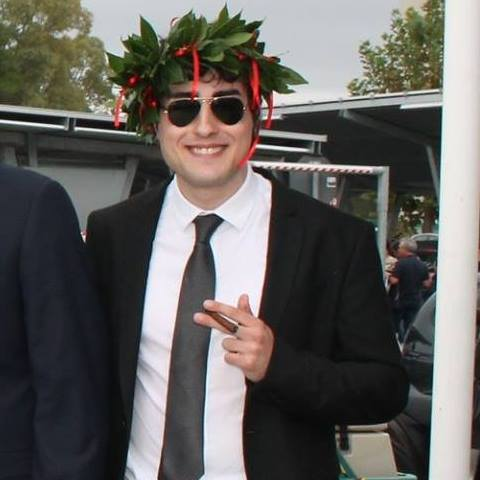
\includegraphics[width=3cm]{figures/marco.jpg}
\vspace{0.3cm}

\raisebox{-0.35ex}{
\includegraphics[width=4ex]{figures/link.png}}%
\hspace{0.05cm} /marcochiarelli

\end{figure}

\begin{figure}[h]

\includegraphics[width=3cm]{figures/gabriele.jpg}
\vspace{0.3cm}

\raisebox{-0.35ex}{
\includegraphics[width=4ex]{figures/link.png}}%
\hspace{0.05cm} /gabrieleaccarino

\end{figure}

\begin{figure}[h]

\includegraphics[width=3cm]{figures/paolo.jpg}
\vspace{0.3cm}

\raisebox{-0.35ex}{
\includegraphics[width=4ex]{figures/link.png}}%
\hspace{0.05cm} /paolo-panarese-6a016187

\end{figure}

\begin{figure}[h]

\includegraphics[width=3cm]{figures/emanuele.jpg}
\vspace{0.3cm}

\raisebox{-0.35ex}{
\includegraphics[width=4ex]{figures/link.png}}%
\hspace{0.05cm} /emanuele-costa-cesari-40ab1211a

\end{figure}


%BIBLIOGRAFIA - redatta con il relativo ambiente
\begin{thebibliography}{100}
\bibitem{rif1} G. Indiveri \emph{Notes on Rotations, Orientation Errors and Robot Kinematics}
\bibitem{rif2} G. Indiveri \emph{Introduzione alla tecnica dei Minimi Quadrati per l'identificazione parametrica e la stima dello stato}
\bibitem{rif3} G. Indiveri \emph{Ph.D Thesis, Chapter 3}
\bibitem{rif4} L. Sciavicco, B. Siciliano \emph{Robotica industriale}
\bibitem{rif5} A. Della Ducata \emph{Notazione di Denavit - Hartenberg}
\bibitem{rif6} L. Fortuna, M. Frasca \emph{Complementi di Teoria dei Sistemi e di Controlli Automatici}
\bibitem{rif7} T. I. Fossen, J. W. \& Sons \emph{Guidance and Control of Ocean Vehicles}
\bibitem{rif8} \emph{Handbook of (Marine) Robotics}
\bibitem{rif9} N. Newman \emph{Marine Hydrodynamics}
\end{thebibliography}

\end{document}


%************************************************
% Chapter 2: ROTAZIONI
%************************************************
% !TEX encoding = UTF-8
% !TEX TS-program = pdflatex
% !TEX root = ../rob.tex
% !TEX spellcheck = it-IT

%************************************************
\chapter{Rotazioni}
\label{cap:rot}
%************************************************\\

\section{Matrici di ROTAZIONE}

L'oggetto matematico che permette di descrivere la posizione di una terna rispetto ad un'altra è la matrice di ROTAZIONE.

\begin{defn}{\textbf{Matrice di ROTAZIONE}}

Dati due sistemi di riferimento $\{<0>,\ <1>\}$ indicati rispettivamente dalla seguente coppia di terne di versori mutuamente perpendicolari: $\{(i_0,j_0,k_0),\ (i_1,j_1,k_1)\}$, definiamo \textit{matrice di rotazione} tra il sistema $<0>$ ed il sistema $<1>$ (l'ordine di enunciazione delle terne è importante) il seguente oggetto matematico:

\[
	^1R_0 =
	\begin{bmatrix}^1i_0\in\R^{3\times 1}&^1j_0\in\R^{3\times 1}&^1k_0\in\R^{3\times 1}\end{bmatrix}
\]

dove, come graficamente esposto, i singoli elementi trascritti nella matrice sono dei vettori colonna. Ognuno di essi rappresenta il versore $i$-esimo, $i=1,2,3$ della terna $<0>$ espresso in terna $<1>$.

\end{defn}

Notiamo che:

\[
	\left\{
	\begin{aligned}
	&^0i_0 =  \begin{bmatrix}1&0&0\end{bmatrix}^\top\\
	&^0j_0 =  \begin{bmatrix}0&1&0\end{bmatrix}^\top\\
	&^0k_0 =  \begin{bmatrix}0&0&1\end{bmatrix}^\top
	\end{aligned}
	\right.
\]

$i_0$ è un versore. Oggetto di grandezza unitaria (in norma), il quale esiste a prescindere dalle sue componenti! I tre numeri conservano la MEMORIA in cui li ho calcolati. La matrice descrive l'assetto. Utile perché se conosco un vettore in una terna e voglio calcolare le sue componenti in terna $<1>$, è sufficiente effettuare questa operazione:

\[
	^1p =\ ^1R_0\ ^0p
\]

\`E semplicemente un prodotto matrice vettore. Ricordiamo che tale operazione è sostanzialmente una combinazione lineare degli elementi di una matrice (colonne) pesati con coefficienti forniti dal vettore con il quale si intende essa moltiplicare:

\[
	y = Mx = x_1m_1 + x_2m_2 +\ \dots\ + x_nm_n
\]

Una tale matrice di rotazione esprime l'assetto. Come è orientata la terna $<0>$ in terna $<1>$? Se prendiamo una direzione nota in terna $<0>$, e vogliamo vedere a cosa quella direzione corrisponde in terna $<1>$, è sufficiente utilizzare: $[^1p =\ ^1R_0\ ^0p]$, che corrisponderebbe alla proiezione in terna $<1>$ del vettore $^0p$. Quindi:

\[
	^1R_0 =
	\begin{bmatrix}{^1}i_0\in\R^{3\times 1}&^1j_0\in\R^{3\times 1}&^1k_0\in\R^{3\times 1}\end{bmatrix}
\]

Ovviamente, per via della disuguaglianza triangolare, ogni colonna deve sommare ad 1 in norma. Per essere una matrice di rotazione, i suoi elementi non saranno MAI maggiori di 1 in modulo! Tabellina di 9 numeri. Se li mettessimo random, molto probabilmente non otterremmo una matrice di rotazione! Ciascuna colonna ha esattamente NORMA 1! (Sono VERSORI!). Abbiamo tre $(1+1+1)$ vincoli relativi alla norma dei versori più tre altri vincoli $(1+1+1)$ relativi al fatto che, rispettivamente: $\{i\perp j,\ j\perp k,\ i\perp k\}$. Tabella di 9 numeri vincolata da 6 equazioni. Ne rimangono 3 altri gradi di libertà, pari quindi al numero di parametri minimi necessari a descrivere univocamente una matrice di rotazione. Rappresentazione minima: servono 3 numeri indipendenti (minimo) per (de)scrivere una matrice di rotazione. Come scegliere questi tre numeri è una storia abbastanza lunga. Alcuni ne scelgono 4 numeri al posto di 3 (QUATERNIONI). Altra caratteristica (tipicamente interconnessa alle altre): $^1p$ è una copia di $^0p$ MA in un altro sistema di riferimento. Ovviamente le componenti / orientazioni cambiano, ma la NORMA no! Dal punto di vista delle componenti, la NORMA di un vettore NON ha bisogno di loro! \`E semplicemente una funzione definita in maniera assiomatica, quindi una distribuzione in tal senso:

\[
	\norma{x}:\R^n\mapsto \R\ |\\
	\left\{
	\begin{aligned}
	&\norma{x} \geq 0,\ \norma{x} = 0 \iff x=0\\
	&\norma{x+y} \le \norma{x}+\norma{y}
	\end{aligned}
	\right.
\]

\`E in realtà a nostra discrezione come definirla! Se questa "turca" funzione soddisfa alle seguenti condizioni, allora è una norma! La norma euclidea è una qualsiasi norma possibile tra le tante (infinite). \`E calcolabile comodamente mediante l'utilizzo delle componenti:

\begin{corl}{\textbf{Calcolo della norma di un vettore mediante componenti}}

\[
	[\norma{x}^2 = X_x^2 + X_y^2 + X_z^2]
\]

\end{corl}

Ma anche le norme, ovviamente, prescindono anch'esse dalle componenti dei vettori. Infatti una definizione più pragmatica e rigorosa è la seguente, della quale il risultato precedente è infatti un corollario:

\begin{defn}{\textbf{Norma di un vettore}}

\[
	[\norma{p\in\R^{3\times 1}}_2 = \sqrt{p^\top p}]
\]

\end{defn}

Proviamo ad applicare la seguente definizione al vettore: $^1p$:

\[
	\norma{^1p}^2 =\ ^1p^\top\ ^1p =\ ^0p^\top\ ^1R_0^\top\ ^1R_0\ ^0p \stackrel{ISOMTRC}{=}\ ^0p^\top\ ^0p = \norma{^0p}^2
\]

Risultato che mostra che la matrice di rotazione esprime una trasformazione ISOMETRICA. Questo risultato naturalmente, wlog, vale $\forall\ ^1p$! Ciò significa che:

\begin{defn}{\textbf{Unitarietà di una matrice di rotazione}}

\[
	^1R_0^\top\ ^1R_0 = I_{3\times 3}
\]

\begin{itemize}
\item La matrice $^1R_0$ è INVERTIBILE! Ovvero ha sempre rango pieno;
\item La sua inversa concide con la TRASPOSTA. (Definizione di matrice unitaria, la quale in campo complesso indica che l'inversa coincide con la TRASPOSTA (COMPLESSA) CONIUGATA, mentre in campo reale indica proprio la definizione appena esplicitata, e si parla di matrice ORTONORMALE).
\end{itemize}

\end{defn}

Le MATRICI UNITARIE, come appena visto, sono \underline{isometriche}. Le operazioni isometriche (lineari, descritte da matrici), sono sicuramente legate a MATRICI UNITARIE. Se lo pensiamo in termini di definizione di $^1R_0$, allora il risultato è OVVIO!

\[
	^1R_0^\top\ ^1R_0 =
	\begin{bmatrix}^1i_0^\top\ ^1i_0 = 1 & 0 & 0\\0 & ^1j_0^\top\ ^1j_0 = 1 & 0\\0 & 0 & ^1k_0^\top\ ^1k_0 = 1\end{bmatrix} = I_{3\times 3}
\]

Adoperiamo ora l'applicazione del teorema di Binet sul determinante di un prodotto: per una matrice quadrata, abbiamo che il determinante della matrice prodotto è pari al prodotto dei determinanti delle singole matrici. Inoltre sappiamo che il determinante della matrice trasposta è pari al determinante della matrice in esame. Mettendo insieme ambo le cose, otteniamo:

\[
	(\det{R})^2 = 1 \implies \det{R} = \pm 1
\]

Il determinante di $R$ è quindi: $\{+1,\ -1\}$. Tutte le matrici unitarie hanno determinante di valore assoluto pari ad 1. Riassumiamo quindi i seguenti fatti:

\begin{itemize} 

\item Tutte le matrici unitarie hanno sicuramente $(\det{R})^2 = 1$;
\item Le ROTAZIONI hanno determinante della matrice di rotazione pari a $(+1)$;
\item Le RIFLESSIONI (quando ci guardiamo allo specchio es.) hanno determinante pari a $(-1)$.

\end{itemize}

Non esiste difatti una rotazione che possa eseguire il mapping relativo ad un'operazione di riflessione. Anche le RIFLESSIONI però conservano la norma, sono quindi pure loro delle isometrie. Supponiamo ora di avere: $h\in\R\ |\ \norma{h}=1$ un versore (vettore di norma unitaria). Consideriamo la seguente matrice di trasformazione:

\[
	Q = I_{3\times 3} - 2hh^\top
\]

Proviamo ad applicarla ad un vettore $v$:

\[
	Qv = (I_{3\times 3} - 2hh^\top)v = v - 2hh^\top v
\]

\begin{itemize}

\item Se $v=h \implies Q(v=h) = -h$ (il vettore $h$ semplicemente cambia segno);
\item Se $(v\perp h \iff v^\top h=h^\top v=0) \implies Qv = v$;

\end{itemize}

Supponiamo di avere un vettore $h = \begin{bmatrix}1&2&7\end{bmatrix}^\top$. Abbiamo che:

\[
	hh^\top = \begin{bmatrix}1&2&7\end{bmatrix}^\top \begin{bmatrix}1&2&7\end{bmatrix} = \begin{bmatrix}1&2&7\\2&4&14\\7&14&49\end{bmatrix}
\]

Notiamo che tale matrice è simmetrica, ma ovviamente si poteva già vedere dal fatto che: $(2hh^\top)^\top = 2hh^\top$. Calcoliamo ora:

\[
	Q^\top Q = (I-2hh^\top)^\top (I-2hh^\top) = I - 2hh^\top - 2hh^\top + 4h(h^\top h = 1)h^\top = I_{3\times 3}
\]

$Q$ è una matrice simmetrica $\impliedby Q^\top = Q$. $Q$ è un'ISOMETRIA. Questa matrice $(Q\in\R^{3\times 3})$ conserva la norma, la lunghezza. $h$ è arbitrario. Basta che sia un versore, a norma 1. NON tutte le ISOMETRIE sono delle rotazioni! Prende un vettore e cambia soltanto il segno delle componenti lungo l'asse ortogonale al piano! Questa è proprio una riflessione!

La trasformata risultante è: trasforma una terna destrorsa in una sinistrorsa. $\nexists$ modo di ruotare una terna per far diventare una terna destrorsa in una sinistrorsa. $(\det{Q}=-1)$. Non tutte le matrici ISOMETRICHE sono delle rotazioni. Esistono operazioni isometriche che non sono delle rotazioni, come appena visto.

$A^\top A = I \implies A$ ISOMETRIA. Tutte le matrici ISOMETRICHE in $\R^n$ hanno determinante della matrice associata $+1$ o $-1$. Le ROTAZIONI sono delle isometrie particolari a determinante $(+1)$.

\begin{defn}{\textbf{Gruppo delle MATRICI ORTONORMALI}}

\[
	\underline{\Theta(n)} = \{M\in\R^{n\times n}\ |\ MM^\top = M^\top M = I_{n\times n}\}
\]

\end{defn}

Prendiamo un paniere delle tali matrici appena definite. Il termine sottolineato è l'insieme delle matrici ortonormali in $\R^n$. Tale oggetto è un gruppo. Gode delle proprietà di gruppo:

\begin{itemize}

\item $\exists$ elemento unitario;
\item Il gruppo è chiuso rispetto al prodotto;
\item associatività (possiamo "spostare" le parentesi).

\end{itemize}

Con i gruppi si può astrarre, ed ottenere delle proprietà particolari per degli oggetti che siano gruppi. $\Theta(n)$ è il gruppo delle trasformazioni isometriche. Un generico elemento che vi appartiene ha determinante $\{+1,\ -1\}$. Lì dentro ci sono pure le rotazioni.

\begin{defn}{\textbf{Gruppo delle rotazioni $\SO(n)$}}

\[
	\SO(n) = \{M\in\R^{n\times n}\ |\ M^\top M = MM^\top = I_{n\times n},\ \underline{\det{M}} = +1\}
\]

\end{defn}

Sicuramente tali matrici sono delle matrici di ROTAZIONE. Matrici speciali ortonormali di ROTAZIONE in $\R^n$. \underline{MATRICI ISOMETRICHE} a determinante $(+1)$; (conservano le lunghezze). $\SO(n)$ è ANCORA UN GRUPPO! Fondamentale. Due matrici di rotazione diverse, se moltiplicate, restituiscono in output una matrice ancora appartenente al gruppo. Eredita quindi l'elemento identico di $\Theta(n)\ (I_{n\times n}\in\R^{n\times n})$. Esiste l'INVERSA, e coincide con la TRASPOSTA, dato che le matrici in gioco sono unitarie. 

Ricordiamo ora le proprietà delle trasformazione di riflessione:

\[	
	\left\{
	\begin{aligned}
	&Qh = -h\\
	&Qv = v \impliedby (v\perp h)
	\end{aligned}
	\right.
\]

Ricordiamo che: $^1p =\ ^1R_0\ ^0p$. Definiamo ora l'operazione di PROIEZIONE:

\begin{defn}{\textbf{\underline{OPERATORE PROIETTORE}}}

with: $h\in\R^{n\times n},\ \norma{h}=1$:

\[	
	M = I_{n\times n} - hh^\top
\]

\end{defn}

Con la seguente matrice prendiamo un versore in $\R^n$ (vettore di norma 1) e ne tagliamo tutte le componenti lungo $h$. Abbiamo:

\begin{itemize}

\item $Mh = 0$;
\item $M(v\perp h) = v$;

\end{itemize}

In un problema di CINEMATICA è scomodo portarsi dietro una matrice di 9 numeri. Solo 3 numeri SONO indipendenti! \`E più comodo manipolare non tutti gli elementi della matrice, ma solo i parametri MINIMI! La Scelta è però NON univoca. $\exists\infty$ modi per individuare tre parametri per descrivere una data matrice di rotazione. Bisogna introdurre una rappresentazione, la RAPPRESENTAZIONE ESPONENZIALE delle matrici di ROTAZIONE. Solo in $\R^3$ (In $SO(3)$ i suoi elementi possono essere rappresentati in tal modo).

\subsection{Matrici simmetriche / antisimmetriche} 

\begin{thrm}{\textbf{Decomposizione simmetrica/antisimmetrica di una matrice}}

\[
	[(M\in\R^{3\times 3}) = \frac{M+M^\top}{2} + \frac{M-M^\top}{2}]
\]

\end{thrm} 

\`E un risultato interessante perché il primo termine è SIMMETRICO (matrice uguale alla sua trasposta $\iff A=A^\top$), mentre è ANTISIMMETRICO il secondo (matrice uguale a MENO la sua trasposta $\iff A=-A^\top$).

Le matrici ANTISIMMETRICHE hanno una proprietà molto particolare. Mappano i vettori in tal modo:

\[
	x^\top (Ax) \stackrel{REAL}{=} (x^\top Ax)^\top \stackrel{TRANSP}{=} x^\top A^\top x \stackrel{SKEWSYMM}{=} -x^\top(Ax) = 0
\]

ove come annotato sopra l'uguale, esso vale dal momento che $(x^\top Ax)\in\R\ \forall A\in\R^{n\times n}$. Le matrici ANTISIMMETRICHE mappano il vettore ($A$ potrebbe pure non essere isometrica ovviamente) ortogonalmente ad esso. Le matrici ANTISIMMETRICHE in $\R^{n\times n}$ godono di questa particolare proprietà.

\subsection{Skew-symmetry}

Teniamo a mente la seguente:

\[	
	M\in\R^{n\times n}\ |\ M = \frac{M+M^\top}{2} + \frac{M-M^\top}{2}
\]

Posti $a,b\in\R,\ c=a\times b \leftarrow$ (operazione lineare). 

\[
	c\mapsto \begin{vmatrix}i&j&k\\a_1&a_2&a_3\\b_1&b_2&b_3\end{vmatrix} = \underline{i}(a_2b_3 - a_3b_2) - \underline{j}(a_1b_3 - a_3b_1) + \underline{k}(a_1b_2 - a_2b_1)
\]

Gli elementi di quella matrice sono associati a componenti del vettore. Abbiamo:

\[
	S(\underline{a}\in\R^{3\times 1})\in\R^{3\times 3}
\]

Matrice $\R^{3\times 3} \ni S(\underline{a})$ che rappresenta l'operazione di prodotto vettore (se opportunamente moltiplicato per un altro vettore, opportuno). Matrice ANTISIMMETRICA. $\underline{a}$ si chiama anche VETTORE ASSIALE della matrice ANTISIMMETRICA. Qualsiasi matrice antisimmetrica ha associato un UNICO vettore assiale. Il modo banale di vederlo è che, prendendo una qualsiasi matrice random, estraendone la parte antisimmetrica $(\frac{M-M^\top}{2})$, ha sempre 0 sulla diagonale principale. Scegliendo a caso $\{a_1,\ a_2,\ a_3\}$, allora abbiamo quindi la corrispondenza: VETTORE ASSIALE $\leftrightarrow$ MATRICE ANTISIMMETRICA. Quei 3 numeri li interpretiamo come componenti del vettore assiale associato. Dimostrazione sulle dispense più efficiente (non passa per le componenti). In realtà un OPERATORE LINEARE prescinde anch'esso dalle componenti! Ha delle particolari proprietà. La dimostrazione si può fare senza fare uso delle componenti! Il prodotto vettore in $\R^3$ definisce un unico vettore assiale di una matrice antisimmetrica (e viceversa). Il risultato di $Ax$ è esprimibile mediante prodotto vettore, e viceversa:

\begin{thrm}{\textbf{Skew-symmetry Matrix and Axial Vector Mapping}}

\[
	\left\{
	\begin{aligned}
	&Ax = a\times x\\
	&a,x\in\R^{3\times 1}\\
	&(A=-A^\top)\in\R^{3\times 3}
	\end{aligned}
	\right.
\]

\end{thrm}

Dimostrazione costruttiva, senza componenti. Obiettivo: Dimostrare che $A$ è ANTISIMMETRICA: $\exists! \underline{a}\ |\ Ax=\underline{a}\times \underline{x}$. Utilizzando le componenti è abbastanza banale, già dimostrato.

\begin{proof}

\[
	\underline{a} = \frac{1}{2}\sum_{i=1}^3{e_i\times Ae_i} = (\dots)
\]

Bisogna applicare le proprietà del prodotto vettore, e ad un certo punto ovviamente la proprietà di antisimmetria per $A$. Chiamiamo con $e_i$ il generico versore $i$-esimo dello spazio $\R^3$ (individuiamo una base ortonormale arbitraria di $\R^3$). Segue:

\[
	\underline{a}\times\underline{x} = \underline{\frac{1}{2}[\sum_{i=1}^3{(e_i\times Ae_i)]}}\times\underline{x} = \frac{1}{2}\sum_{i=1}^3{(\underline{x}\times(Ae_i\times e_i))} = (\dots)
\]

Ove abbiamo cambiato l'ordine del prodotto vettore due volte onde evitare il segno. Si rammenti la regola del TRIPLO PRODOTTO:

\[
	a\times(b\times c) = b(a^\top c) - c(a^\top b)
\]

Sempre vera. L'ordine nel prodotto vettore conta! Si effettui prima $(b\times c)$, e lo si moltiplichi secondo prodotto vettore per $\underline{a}$. Quindi, tornando a noi:

\[
	(\dots) = \frac{1}{2}\sum_i{[\underline{(Ae_i)(x^\top e_i)} - e_i(x^\top Ae_i)]} = (\dots)
\]

Ove il termine sottolineato sommato ad $i$ restituisce proprio $Ax$, per definizione. Ora applichiamo l'antisimmetria.. se anziché $x^\top Ae_i$ ne mettessimo la versione invertita, allora esso cambierebbe segno. Fino ad ora abbiamo fatto semplicemente del calcolo generico.

\[
	(\dots) \stackrel{SKEWSYMM}{=} [\frac{1}{2}(Ax + \underline{\sum_i{e_i((Ax)^\top e_i)}}] = \frac{Ax}{2}+\frac{Ax}{2} = Ax
\]

\end{proof}

Ove il termine sottolineato è sempre $Ax$. Ciò chiude la dimostrazione. Questo vettore assiale $\underline{a}$ è UNICO! Dimostrazione semplice per esercizio. Non è molto standard, ma l'operazione che mappa una matrice antisimmetrica nel suo vettore assiale è la seguente, definita mediante il seguente mapping:

\[
	\Vex(A) = \underline{a}\in\R^{3\times 1}
\]

Abbastanza pesante come notazione, ma non infrequente in letteratura. Pseudo-vettore in realtà. Nell'ambito delle rotazioni il vettore assiale lo incontreremo abbastanza di frequente. $\underline{a}=\begin{bmatrix}a_1&a_2&a_3\end{bmatrix}^\top$. La matrice $A$, è quindi:

\[
	A := S(\Vex(A)) = S(\underline{a}) =
	\begin{bmatrix}0&-a_3&a_2\\a_3&0&-a_1\\-a_2&a_1&0\end{bmatrix}
\]

Se una tale matrice $A$ fosse ad esempio: $A:=\begin{bmatrix}0&3&2\\-3&0&-1\\-2&+1&0\end{bmatrix}$, allora il suo vettore assiale sarebbe: $Vex(A):=\underline{a}=\begin{bmatrix}1&2&-3\end{bmatrix}^\top$. Sul segno vi è in realtà un po' di ambiguità, ma non relativamente al vettore assiale in sé per sé.

La regola del triplo prodotto è stata molto utile, e sarà tale ancora durante il prosieguo del corso:

\begin{thrm}{\textbf{Regola del TRIPLO PRODOTTO}}

\[
	\underline{a}\times(\underline{b}\times\underline{c}) = \underline{b}(a^\top c) - \underline{c}(a^\top b) = (\dots)
\]

\end{thrm}

Questo fatto mette in evidenza che questa operazione tra vettori, ne freeza due e tratta il terzo come parametro (costante); l'operazione è quindi lineare. Banale dimostrarlo:

\[
	[(\dots) = (I_{3\times 3}(a^\top c) -\underline{c}\underline{a}^\top \in\R^{3\times 3})\underline{b}]\in\R^{3\times 1} = (\dots)\\
\]

Rispetto $\underline{b}$ lo posso scrivere come matice per $\underline{b}$. Se fossero $\underline{a}$, o $\underline{c}$ liberi, avremmo:

\[
	\left\{
	\begin{aligned}
	&(\dots);\\
	&(\dots) = (\underline{b}\underline{c}^\top -\underline{c}\underline{b}^\top)\underline{a};\\
	&(\dots) = [\underline{b}\underline{a}^\top -I_{3\times 3}(\underline{a}^\top\underline{b})]\underline{c};
	\end{aligned}
	\right.
\]

Operatore lineare su uno dei tre argomenti. Su qualche passaggio cinematico tornerà utile. Regola del triplo prodotto banalmente dimostrabile per calcolo diretto. Mostriamo un po' di \emph{sugar calculus}:

\[
	\left\{
	\begin{aligned}
	&\{\Vex(A),\ \underline{S^\top(\underline{a}) = -S(\underline{a})}\}\\
	&[\Vex(A)=\underline{a} \implies \Vex[S(\underline{a})] = \underline{a}]
	\end{aligned}
	\right.
\]

\subsubsection{Proprietà di una Matrice Antisimmetrica}

\`E utile sapere che la potenze di una matrice antisimmetrica hanno una particolare ricorsione. Calcolabile di nuovo per calcolo diretto:

\[	
	\{S(\underline{a})S(\underline{a}) := S^2(\underline{a}),\ S(\underline{a})S(\underline{a})S(\underline{a}) := S(\underline{a})^3,\ \dots\}
\]

Ad occhio vengono fornite le seguenti formule. Dato: $\underline{h}\in\R^{3\times 1}\ |\ \norma{h}=1$ VERSORE, abbiamo:

\[
	\left\{
	\begin{aligned}
	&S(\underline{h}) = \underline{h}\times\mathord{\cdot}\\
	&S^2(\underline{h}) = hh^\top - I_{3\times 3}\\
	&S^3(\underline{h}) = -S(\underline{h})\\
	&S^4(\underline{h}) = -S^2(\underline{h})
	\end{aligned}
	\right.
\]

Possiamo generalizzare:

\begin{thrm}{\textbf{Potenze di una MATRICE ANTISIMMETRICA}}

\[
	\left\{
	\begin{aligned}
	&S^{2i+1}(\underline{h}) = (-1)^iS(\underline{h})\\
	&S^{2(i+1)}(\underline{h}) = (-1)^i(\underline{hh^\top -I_{3\times 3}})
	\end{aligned}
	\right.
\]

\end{thrm}

Ricordiamo che $(I_{3\times 3} - hh^\top)$ è il proiettore. Quindi il termine sottolineato è il proiettore cambiato di segno. Per alcune potenze pari (precisamente le potenze pari di esponente $i$ dispari), sarà proprio il proiettore, per le altre sarà il proiettore cambiato di segno, per l'appunto.

$S(\underline{h})v=h\times v,\ \Tr(S(\underline{h})=0)$. La traccia delle potenze dispari continuerà quindi ad essere 0. La traccia delle potenze pari, data la traccia particolare che $hh^\top$ esibisce ovvero $\Tr(hh^\top) = h^\top h=1$, ha la seguente espressione:

\[
	[\Tr(S^{2(i+1)}(\underline{h})) = (-1)^{i+1}2]
\]

Ulteriore proprietà: stupidaggine ma fino ad un certo punto: verrà comoda più in avanti. \`E la seguente: $\forall$ matrice antisimmetrica $\mathord{\cdot}\in\{\R^{3\times 3}\}$ è associato un UNICO VETTORE ASSIALE!

Ora prendiamo $\{\exists M\in\R^{3\times 3},\ \underline{x}\in\R^{3\times 1}\}$.
Eventualmente $M$ può anche essere a simmetria non ben definita. Calcoliamo la trasposta della matrice ottenuta a valle dell'applicazione della trasformazione di similitudine:

\[
	(M\underline{S(\underline{x})}M^\top)^\top = MS(\underline{x})^\top M^\top = -MS(\underline{x})M^\top
\]

$\implies [MS(\underline{x})M^\top]$ antisimmetrica! Essendo antisimmetrica, deve ammettere un vettore assiale: 

\begin{thrm}{\textbf{Trasformazione di similitudine di una Matrice Antisimmetrica}}

\[
	\left\{
	\begin{aligned}
	&MS(\underline{x})M^\top = S(\underline{y})\\
	&y = (L\in\R^{3\times 3})x
	\end{aligned}
	\right.
\]

\end{thrm}

$(L\in\R^{3\times 3})$ è stata già calcolata. Usiamo la notazione \emph{MATLAB}, ove $M(2,:)$ indica la seconda riga (quindi in versione trasposta rappresenterebbe un vettore colonna); ad esempio il termine citato prima corrisponde alla riga selezionata della matrice $M$ così parametrizzata:

\[
	\begin{bmatrix}m_{11}&m_{12}&m_{13}\\\underline{m_{21}}&\underline{m_{22}}&\underline{m_{23}}\\m_{31}&m_{32}&m_{33}\end{bmatrix}
\]

abbiamo:

\[
	L = \begin{bmatrix}\begin{bmatrix}M(2,:)^\top\times M(3,:)^\top\end{bmatrix}^\top\\\begin{bmatrix}M(3,:)^\top\times M(1,:)^\top\end{bmatrix}^\top\\\begin{bmatrix}M(1,:)^\top\times M(2,:)^\top\end{bmatrix}^\top\end{bmatrix}
\]

$M$ è la più generale possibile. Se prendiamo per $M$ un elemento di $\SO(3)$ (matrice di rotazione), la $L$ associata è proprio $M$! Ovvero la tale matrice di rotazione scelta. A valle dell'analisi, del tutto generale, ricaviamo un utilissimo risultato particolare. Prendiamo una generica matrice di rotazione:

\begin{corl}{\textbf{Trasformazione di similitudine di una Matrice Antisimmetrica}}

$R\in\SO(3),\ \forall x\in\R^{3\times 1}$:

\[
	[RS(\underline{x})R^\top = S(Rx)]
\]

\end{corl}

\`E un risultato abbastanza semplice. Dal punto di vista algebrico è come abbiamo detto prima. In $\SO(3),\ L=R$. Un interpretazione geometrica è molto profonda. Una rotazione, dal punto di vista geometrico, è un'ISOMETRIA (che CONSERVA le distanze), che conserva il PRODOTTO VETTORE. Le rotazioni fanno sì che le distanze relative tra due punti fissi rimangano uguali! Trasformazione di similitudine:

\[
	\underline{RS(\underline{x})R^\top = S(R\underline{x})}
\]

$\leftarrow$ le rotazioni conservano il prodotto vettore: ruotando il risultato del prodotto vettore è la stessa cosa del ruotare singolarmente, isolatamente l'operando sinistro di esso (del prodotto vettore). \`E un risultato in realtà abbastanza potente!

Possiamo adesso analizzare un legame profondo e significativo tra gli elementi di $\SO(3)$ e le \underline{matrici esponenziali}:

\subsection{Matrici ESPONENZIALI}

\begin{defn}{\textbf{Matrice ESPONENZIALE}}

$M\in\R^{n\times n}\ \theta\in\R,\ \forall i,j$

\[
	(L = \e^{M\theta}\in\R^{n\times n}) := (\underline{\sum_{l=0}^{+\infty}{\frac{M^l\theta^l}{l!}}}) < +\infty \iff e^{M\theta}_{ij} <+\infty
\]

\end{defn}

Tale matrice è nientemeno che la matrice $e^{At}$ vista in TdS. $\e$ è proprio il simbolo di Nepero in tal caso, ma stavolta rappresenta una matrice intesa come autofunzione rispetto ad operatori differenziali, come vedremo dalle prossime proprietà.
La sommatoria tra parentesi tonde CONVERGE sicuramente! La sommatoria rappresenta infinite potenze, scalate per $\frac{1}{l!}$ e sommate. Converge ad una quantità finita, ovvero in tal caso ad una matrice con elementi tutti finiti. Come già anticipato, il motivo per cui utilizziamo questa notazione è che, non solo ricorda Taylor, ma questa matrice qui gode di parecchie proprietà, molte delle quali analoghe a quelle dell'esponenziale scalare.

\subsubsection{Proprietà della Matrice Esponenziale}

Dal punto di vista concettuale le seguenti proprietà sono molto profonde:

\begin{itemize}

\item La matrice $\e^{M\theta}$ è sempre INVERTIBILE, $\forall M$ anche NON INVERTIBILE!
\item Al posto di $M$, mettendovi $-M$, ed eseguendo l'esponenziale matriciale otteniamo l'inversa di $(\e^{M\theta})$:
$\inv{(\e^{M\theta})} = \e^{-M\theta}$;
\item $(\e^{M\theta})^\top = \e^{M^\top\theta}$;
\item $[\underline{M\e^{M\theta} = \e^{M\theta}M}]$.

\end{itemize}

Le matrici generiche tra di loro non commutano generalmente rispetto al prodotto matriciale. L'ultima proprietà è un risultato abbastanza stupido: si ottiene semplicemente moltiplicando per $M$ ambo i membri della definizione, e vedendo cosa si ottiene nell'RHS..

La matrice non è tuttavia banale da calcolare generalmente. Una delle sue possibili difficoltà è che le potenze non hanno una struttura semplice o ben definita. Ci sono alcuni casi invece semplici e banali, ad esempio nel caso di matrici $M$ NILPOTENTI (dopo alcune potenze diventano 0) oppure IDEMPOTENTI. Se è diagonalizzabile ci sono invece altri trucchi, legati alla costruzione delle cosiddette matrici di JORDAN, LAPLACE, etc.. Se $l=17$, abbiamo 17 termini nella sommatoria matriciale.

Notazioni matematiche: $\{\{h\in\R^{3\times 1},\ \norma{h}=1\},\ SCALAR\ \theta\in\R\}$. Calcolando:

\[
	[\underline{\e^{\theta S(\underline{h})} \in\R^{3\times 3}}] \in\SO(3)
\]

Vi è un legame SURGETTIVO sostanzialmente. Vale un risultato fondamentale, dimostrato da Eulero nel 1700. Possiamo ricoprire tutto $\SO(3)$. $\forall$ elemento di $\SO(3)$, ammette tanti $\theta,\ \underline{h}$ tale per cui valga l'appartenenza al gruppo prima esplicitata. La ricopertura è addirittura troppo buona! Nel senso che, vi sono diversi modi (parametri) per giungere allo stesso elemento di $\SO(3)$, come vedremo più in avanti.

\subsubsection{Rappresentazione esponenziale delle Matrici di Rotazione}

Tale sottosezione è di una notevole importanza pratica! Praticamente ENORME! Non solo dal punto di vista teorico. Tale formula tuttavia non ci dice ancora niente. Proprio perché la matrice esponenziale è difficile da calcolare $(\e^{\theta S(\underline{h})})$. In realtà quella formula si può semplificare (RODRIGUES). Dobbiamo dimostrare anzitutto che:

\begin{thrm}{\textbf{Appartenenza ad $\SO(3)$ delle Matrici Esponenziali (Speciali)}}

\[
	[\e^{\theta S(\underline{h})}\in\SO(3)]
\]

\end{thrm}

\begin{proof}


\begin{itemize}

\item{\textit{Unitarietà della matrice}}:

\[
	(\e^{\theta S(\underline{h})})^\top(\e^{\theta S(\underline{h})}) \stackrel{EXP}{=} \e^{\theta S^\top(\underline{h})}\e^{\theta S(\underline{h})} = (\dots)
\]
\[
	(\dots) = \e^{\theta (S^\top(\underline{h}) + S(\underline{h}))} = \stackrel{SKEWSYMM}{=} \e^{\theta(-S(\underline{h})+S(\underline{h}))} \stackrel{EXPINV}{=} I_{3\times 3}
\]

\item{\textit{Determinante positivo unitario}}:

Abbiamo anche dimostraro che, per Binet, il determinante al quadrato è 1! $(\det(\e^{\theta S(\underline{h})}) = \pm 1)\ \forall\theta\forall h$! Come facciamo a dimostrare che è proprio $+1$ e non $-1$? Il determinante di una matrice è una funzione continua dei suoi elementi. Se sapessimo scrivere $(\e^{\theta S(\underline{h})})$ (i suoi singoli elementi), ci aspetteremmo che essa sia una funzione di 4 numeri, di 4 parametri: $(\begin{bmatrix}h_1&h_2&h_3\end{bmatrix}^\top, \theta)$. Il determinante sarà o costantemente $+1$, o costantemente $-1$. \`E una funzione continua dei suoi parametri. Se prendiamo $(\theta=0)$, abbiamo:

\[
	(\e^{0S(\underline{h})} = I_{3\times 3})
\]

il cui determinante è proprio $(+1)$! In un punto quindi il determinante lo sappiamo calcolare, e lo abbiamo calcolato in maniera esatta. $+1$ ovunque. Relativamente sottile come ragionamento, ma non difficile. Tale risultato, ricapitolando, si ottiene mettendo insieme due cose:

\begin{itemize}

\item Determinante in modulo unitario;
\item Determinante funzione continua degli elementi della matrice.

\end{itemize}

\end{itemize}

\end{proof}

In questa definizione non abbiamo supposto che $h$ fosse un VERSORE. VETTORE GENERICO. Per comodità (wlog), si utilizzerà $h\ |\ \norma{h}=1$.

\subsubsection{Formula di Rodrigues}

Se prendiamo la formula dell'esponenziale matriciale, riscrivendola:

\[
	[\e^{\theta S(\underline{h})} \in\SO(3)]
\]

Mi ricordo della definizione di matrice esponenziale. La riscrivo computandola per esteso, trovando:

\begin{defn}{\textbf{FORMULA DI RODRIGUES}}

\[
	\e^{\theta S(\underline{h})} = I_{3\times 3} + \sum_{l=1}^{+\infty}{\frac{S^l(\underline{h})}{l!}\theta^l} \stackrel{REC.SKEWPOWER}{=} (\dots)
\]
\[
	(\dots) = [I_{3\times 3} + \sin(\theta) S(\underline{h}) + (1-\cos(\theta))S^2(\underline{h})]
\]

\end{defn}

ove si è utilizzato nell'ultimo passaggio della definizione le formule delle potenze di $S(\underline{h})$, trovando il risultato esposto per semplice pura ispezione visiva.

A questo punto la matrice di rotazione la riusciremo a scrivere! Con carta e penna, MATLAB, C, Java, etc. Ad esempio: $\{h\ VERSORE\ |\ \norma{h}=1\},\ \theta=35^{\circ}$. Disponendo quindi dei seguenti elementi: $\{h,\theta\} \leftrightarrow$ \{versore dell'asse, angolo di rotazione\}, riusciamo quindi a scrivere la matrice di rotazione. La formula di Rodrigues è stata quindi ottenuta dal riconoscimento dello sviluppo in serie di Taylor delle funzioni trigonometriche applicato alla scrittura delle varie potenze della matrice antisimmetrica. Va detto che $h$ è il versore dell'asse di rotazione. Dev'essere un autovettore di $R$ con autovalore associato $1$, dal momento che abbiamo la seguente direzione preferenziale:

\[
	(\e^{\theta S(\underline{h})}\underline{h}) = \underline{h}
\]

$h$ è quindi la direzione dell'asse di rotazione. $\theta$ dev'essere necessariamente l'angolo. Ci rimane da chiederci: se prendo un generico elemento di $\SO(3)$, $\exists h\in\R^{3\times 1}\ |\ \norma{h}=1,\ \theta\in\R$ tale per cui esista una matrice esponenziale $\e^{\theta S(\underline{h})}$ che lo rappresenti? Ruotare di $(\theta=0^{\circ})$ vuol dire avere infiniti $h$ (qualsiasi asse possibile). Per scrivere problemi di controllo, ad esempio l'orientazione di un satellite, mi calcolo dei parametri delle posizioni finali. Mi calcolo la \underline{fdt $h(t)$} (se fosse lineare), la quale avrebbe matematicamente una SINGOLARIT\`A. \`E un problema di Rappresentazione, NON problema fisico. Le Rappresentazioni esponenziali delle matrici di rotazione hanno questi problemi (NON-UNIVOCIT\`A, ovvero SINGOLARIT\`A in gioco).

\subsubsection{Mapping SURGETTIVO}

Abbiamo un mapping surgettivo tra la matrice exp e gli elementi in $\SO(3)$. Ricordiamo che:

\[
	\e^{S(\underline{h})\theta} = I_{3\times 3} + \sin(\theta)S(\underline{h}) + (1-\cos(\theta))S^2(\underline{h})
\]

con $\underline{h}\in\R^{3\times 1},\ \norma{h}=1,\ \theta\in\R$. La sopracitata formula di Rodrigues vale $\forall\theta\forall \underline{h}$. Il problema è notare che esistono infiniti $\theta$ e $\underline{h}$ che consentono di individuare elementi in $\SO(3)$. Notiamo che scelto $(\theta\in\R)$, si potrebbe ottenere la stessa matrice exp andando a scalare $\theta$ di un fattore $2k\pi$, giacché le funzioni trigonometriche in gioco sono periodiche di periodo $2\pi$. NB: Il legame tra l'evoluzione temporale di un matrice di rotazione ed i suoi parametri $\{\underline{h},\ \theta\}$ che la descrivono non è banale! Occorre definire il fattore integrante: il vettore velocità angolare. Occorre focalizzarsi sulla posa iniziale e quella finale, ma non si hanno gli strumenti per descrivere la traiettoria.

Ogni matrice quadrata $n\times n$ è decomponibile nella somma di una parte simmetrica e di una antisimmetrica, e questo si evince anche nella formula di Rodrigues. Data una matrice arbitraria $R\in\SO(3)$, abbiamo:

\[
	[\Vex(\frac{R-R^\top}{2}) = \sin(\theta)\underline{h}]
\]

Se calcoliamo la traccia di $\e^{S(\underline{h})\theta}$, noteremo che la parte antisimmetrica non dovrebbe contribuire, dal momento che tale matrice ha tutti 0 sulla diagonale principale.

\[
	\left\{
	\begin{aligned}
	&S^2(\underline{h}) = hh^\top - I_{3\times 3}\\
	&\Tr(S^2(\underline{h})) = -2
	\end{aligned}
	\right.
\]

Eguagliamo ora la traccia di $R$ con quella di $\e^{\theta S(\underline{h})}$:

\[
	\Tr(R) = 3 + 0 -2(1-\cos(\theta)) = 1+2\cos(\theta) \implies
	\left\{
	\begin{aligned}
	&\centernot{2}cos(\theta) = \frac{tr(R)-1}{2}\\
	&\theta h = \frac{\theta}{\sin(\theta)} \Vex(\frac{R-R^\top}{2})
	\end{aligned}
	\right.
\]

Ma la prima equazione del sistema non è $\theta$! Dobbiamo quindi estrarre l'arcocoseno; ma quando lo estraiamo, il modulo è ben definito, ma non il segno! Il problema è che se $\theta=0$, sostituito nella seconda equazione fornisce:

\[
	\Vex(\frac{R-R^\top}{2}) = \sin(\theta)\underline{h} = 0 \implies [R=I]
\]

Non riesco quindi ad individuare un $\underline{h}$ univoco, infatti esso può essere qualsiasi con $\theta=0^{\circ}$! ($\exists\ MUL\ \underline{h}$). L'ambiguità sta in come trattiamo i parametri che sono 4: $\{h_x,\ h_y,\ h_z,\ \theta\}$. Infatti le componenti di $h$ sono dipendenti per la condizione di NORMALIZZAZIONE $\iff \norma{h}=1$; $\underline{h}$ ha due componenti linearmente indipendenti. $\underline{h}$ è un versore, le sue componenti sono scalari, e sono peraltro DIPENDENTI TRA DI LORO! Possiamo inoltre considerare un vettore:

\begin{defn}{\textbf{VETTORE ASSE-ANGOLO EQUIVALENTE}}

\[
	\nu:=\begin{bmatrix}\underline{h}^\top&\theta\end{bmatrix}^\top
\]

Tali sue quattro componenti, con $\norma{h}=1$ risultano essere equivalenti a tre variabili indipendenti. Le prime tre sono quelle di $\underline{h}$, e la quarta è $\theta$.

\end{defn}

Data $R\in\SO(3)$, possiamo calcolare il $\theta$, estraendo direttamente il coseno; Purché $\theta\neq k\pi$ possiamo direttamente calcolare $\theta\underline{h}$:

\begin{defn}{\textbf{Rotation Vector}}

\[
	[\theta\underline{h} = \frac{\theta}{\sin(\theta)}\Vex(\frac{R-R^\top}{2})]
\]

\end{defn}

where $\theta\in(-\pi,+\pi)$. Se abbiamo una rotazione di un multiplo di $\pi$, non abbiamo un solo $\theta\underline{h}$ che definisce univocamente la rotazione. La singolarità quindi non sta in 0, ma in $\pi$, dal momento che la funzione reciproca del $\sinc{\mathord{\cdot}}$ è ben definita in 0 e vale 1.


\begin{defn}{\textbf{Rappresentazioni minime in $\SO(3)$}}

Si chiamano RAPPRESENTAZIONI MINIME in $\SO(3)$ qualsiasi funzione che associa a tre valori indipendenti un elemento in $\SO(3)$. Qualunque essa sia avrà almeno una singolarità.

\end{defn}

In questi casi stiamo considerando delle situazioni in cui una terna di riferimento (es. spigoli del muro) descrive come un oggetto è orientato nello spazio. $\underline{h}$ è l'asse di rotazione: mi dice la direzione attorno alla quale ruoto di $\theta[^{\circ}]$ rispetto al S.R. correntemente in uso.

Eulero afferma che l'assetto finale dell'oggetto poteva essere raggiunto attraverso \newline\underline{UNA SOLA ROTAZIONE}! Rotazione elementare rispetto ad un particolare asse fisso, opportunamente scalato ed orientato secondo un angolo $\theta$; eventualmente anche una traslazione se l'oggetto finale si è mosso. Questa è una caratteristica intrinseca dello spazio euclideo.

Per descrivere un elemento di $\SO(3)$, possiamo utilizzare alternativamente al vettore asse-angolo equivalente altri due angoli: angoli di Eulero ed angoli di Yaw, Pitch e Roll, che sono in realtà \underline{alberi} (TREE) di angoli.

\subsection{Angoli di Eulero, YPR}

\subsubsection{Angoli di Yaw, Pitch e Roll}

L'obiettivo è trovare tre parametri in grado di descrivere un elemento di $\SO(3)$. Possiamo immaginare di usare come parametri gli angoli di rotazione utilizzati per arrivare dalla terna di partenza a quella di arrivo: gli angoli sono linearmente indipendenti, ma devo decidere se misurare la rotazione tutta rispetto a quella \underline{di partenza} (\textit{initial axis}), oppure rispetto a quella \underline{corrente} (\textit{current axis}) (quella nuova), cioè gli assi istantanei. Inoltre le rotazioni finite non contano, ma solo quelle infinitesime. Ricordiamo che:

\[
	\left\{
	\begin{aligned}
	&\begin{bmatrix}X=30^{\circ}&Y=45^{\circ}&Z=0^{\circ}\end{bmatrix}^\top\\
	&\begin{bmatrix}X=45^{\circ}&Y=30^{\circ}&Z=0^{\circ}\end{bmatrix}^\top
	\end{aligned}
	\right.
\]

non descrivono la stessa rotazione! Quindi essi \underline{NON COMMUTANO}! Occorre quindi decidere opportunamente in anticipo l'ordine della sequenza degli angoli $X,Y,Z$, oppure $Y,X,Z$, etc. Se facessimo tre rotazioni indipendenti attorno agli assi principali della terna corrente, parliamo di angoli di Yaw, Pitch e Roll.

Parliamo di angoli di Eulero quando le rotazioni avvengono attorno a sempre a due assi correnti indipendenti. Ad esempio: $\left\{\begin{aligned}&xyx\\&xzx\\&yzy\end{aligned}\right.$. Tutte queste rotazioni atomiche attorno l'asse corrente sono indipendenti purché l'angolo di rotazione dell'asse centrale sia diverso da 0. NB: Non basta dire che YAW è un angolo di rotazione rispetto a $z$, ma a seconda di come metto insieme tutte le rotazioni atomiche possiamo ottenere differenti matrici di rotazione risultanti. Entrambe le famiglie di angoli hanno almeno una singolarità, legata alla dipendenza della rotazione intorno agli assi. Le singolarità devono essere messe tipicamente a $-90^{\circ}$ (pitch), cioè lontane dall'area di lavoro; questo può essere fatto scegliendo opportunamente la sequenza di angoli.

Le rotazioni attorno gli assi $(x,y,z)$ possono finalmente essere rappresentate matematicamente.

\subsection{QUATERNIONI}

Sono vettori di quattro componenti che possono essere utilizzati per aggirare le singolarità di rappresentazione: è singolare il legame tra la matrice di rotazione e gli angoli YPR. Quando un oggetto precipita la sua matrice di rotazione è ben definita, ma non i suoi parametri che dovrebbero identificarla! Quindi se utilizzassi delle matrici non si porrebbe il problema. Il problema delle singolarità è sostanzialmente intrinseco in $\SO(3)$, quindi non c'è speranza di individuare tre parametri che non hanno singolarità di rappresentazione. Allora ne uso quattro! Così non abbiamo problemi. Definiamo:

\[
	\left\{
	\begin{aligned}
	&\mu := \cos(\frac{\theta}{2})\\
	&\underline{\epsilon} := \sin(\frac{\theta}{2})\underline{h}
	\end{aligned}
	\right.
\]

Posta la seguente condizione di NORMALIZZAZIONE: $\mu^2 + \norma{\epsilon}^2 = 1$.
Il primo termine $(\mu\in\R)$ è uno scalare, ed è la parte scalare o reale dei quaternioni, mentre $\epsilon$ è la parte vettoriale od ipercomplessa dei quaternioni. Viene posta la seguente condizione di NORMALIZZAZIONE: $\mu^2 + \norma{\epsilon}^2 = 1$. La ben nota formula di Rodrigues può essere riscritta in termini di $\{\mu,\ \epsilon\}$:

\begin{thrm}{\textbf{Formula di Rodrigues per i QUATERNIONI UNITARI}}

\[
	[R = I_{3\times 3} + 2\mu S(\underline{\epsilon}) + 2S^2(\underline{\epsilon})]
\]

\end{thrm}

\begin{proof}

\[
	R=I_{3\times 3} + \sin(\theta)S(\underline{h}) + (1-\cos(\theta))S^2(\underline{h}) = I_{3\times 3} + 2\sin(\frac{\theta}{2})\cos(\frac{\theta}{2})S(\underline{h}) + 2\sin^2(\frac{\theta}{2})S^2(\underline{h}) = (\dots)
\]
\[
	(\dots) = I_{3\times 3} + 2\mu S(\underline{\epsilon}) + 2S^2(\underline{\epsilon})
\]

\end{proof}

\underline{Non ci sono singolarità}!! In tal caso non considero il vettore $\theta\underline{h}$ (asse-angolo equivalente), ma $\epsilon$! Di conseguenza non abbiamo singolarità né in $\theta=0$ né in $\theta=k\pi$. Infatti:

\[
	\left\{
	\begin{aligned}
	&\{\mu=1,\ \underline{\epsilon}=\underline{0}\},\ \theta=0\\
	&\{\mu=0,\ \underline{\epsilon}=\underline{h}\},\ \theta=\pi
	\end{aligned} 
	\right.
\]

Ogni parametrizzazione minima cioè a tre componenti avrebbe di fatto ALMENO una singolarità.

\subsection{CINEMATICA}

Fino ad ora abbiamo parlato di \underline{rappresentazioni statiche} di terne che ruotano. Quando parliamo di rotazioni qual è l'oggetto che consente di modellare il moto nel tempo? Non sono sufficienti gli angoli di Eulero; a questo scopo viene utilizzato il vettore \underline{velocità angolare}. Sappiamo che $\forall R\in\SO(3),\ RR^\top = I_{3\times 3}$. Cio infatti segue proprio dalla membership definition degli elementi di $\SO(3)$.

\[	
	\forall R\in\SO(3),\ RR^\top = I_{3\times 3} \implies \frac{d}{dt}({^0}R_1\ ^0R_1^\top) = 0 \implies\ ^0\dot{R}_1\ ^0R_1^\top +\ ^0R_1\ ^0\dot{R}_1^\top = 0 \implies
\]
\[
	\implies [{^0}\dot{R}_1\ ^0R_1^\top = -{^0}R_1\ ^0\dot{R}_1^\top = -({^0}\dot{R}_1\ ^0R_1^\top)^\top]
\]

$R$ è sempre una qualsiasi matrice in $\SO(3)$, essa cambia nel tempo $\iff R := R(t)$, in modo tale che $RR^\top=I_{3\times 3}$, ma $^0\dot{R}_1\ ^0R_1^\top$ è \underline{antisimmetrica}. Ma ogni matrice antisimmetrica $3\times 3$ ammette vettore assiale (UNICO peraltro). Quindi:

\begin{defn}{\textbf{Vettore velocità angolare}}

$\exists!\ ^0\omega_{1/0},\ \exists\mu\in\R^{3\times 1}\ |$
\[
	[({^0}\dot{R}_1\ ^0R_1^\top)\ ^0\mu =\ ^0\omega_{1/0}\times\ ^0\mu] \implies \dot{R}R^\top = S(\omega)
\]

\end{defn}

La suddetta equazione è in realtà un'equazione differenziale! Il calcolo dell'assetto successivo $(R)$ necessita di avere $\omega$, infatti solo attraverso l'integrazione di $\dot{R}R^\top$ potremmo ottenere $R$: sarebbe sbagliato interpretare solo $\dot{R}$ come fattore integrante: otterremmo difatti un elemento non in $\SO(3)$.
$\omega$ è detto \underline{fattore integrante}, e non può essere definito tramite derivate di angoli, ma solo in maniera assiomatica attraverso il $\Vex(\mathord{\cdot})$!

\subsection{VETTORE VELOCIT\`A ANGOLARE}

Cinematica delle Rotazioni. Definizione del vettore velocità angolare:

\[
	\left\{
	\begin{aligned}
	&R\in\SO(3)\\
	&\dot{R}R^\top = S(\omega)
	\end{aligned}
	\right.\implies [\Vex(\dot{R}R^\top) :=\ ^0\omega_{1/0}]
\]

$\dot{R}R^\top\in\R^{3\times 3}$ è antisimmetrica. Quindi $\exists! \Vex(\dot{R}R^\top)$ tale che faccia valere le precedenti relazioni. Tale è il vettore velocità angolare. Etichetta $a/b$. Etichetta che la matrice $R$ mappa due terne $<A>$ e $<B>$ tramite mapping 1-1, biunivoco. Corrispondente del vettore con componenti in terna $<B>$ espresso in funzione del frame $<A>$ (proiettato). Ricordiamo che: $^AR_B = \begin{bmatrix}^Ai_B&^Aj_B&^Ak_B\end{bmatrix}$. Se le due terne non sono ferme tra di loro, evidentemente $(\dot{R}\neq 0) \implies$ potremmo quindi scrivere l'equazione:

\[
	^A\dot{R}_B\ ^AR_B^\top = S({^A}\omega_{B/A})
\]

Pedici $B$ pesanti ma espliciti. $B/A$ indica che quella è la velocità angolare della terna $<B>$ rispetto ad $<A>$, espressa nel frame $<A>$. Dal punto di vista della notazione, nomenclatura, l'equazione $[\dot{R}R^\top = S(\omega)]$ viene in letteratura chiamata \underline{\underline{STRAP-DOWN} EQUATION}, ove il termine doppiamente sottolineato indica letteralmente legame, legatura. \`E stata iniziata ad essere utilizzata (è stata definita sempre da Eulero) negli algoritmi di navigazione, con le complicazioni aerospaziali degli anni '60 (Assetto di un aeroplano, per controllarlo). Componenti della velocità angolare a bordo del veicolo. Come sta cambiando l'orientamento rispetto ad una terna assoluta? L'osservatore dello Stato per determinare $\omega$, viene fatto mediante Filtro Osservatore. Nome in ambito di navigazione. Da questa relazione di base, soltanto una definizione, si possono dedurre delle fondamentali proprietà della velocità angolare.

\subsubsection{Proprietà del vettore Velocità Angolare}

Gode della proprietà di COMPOSIZIONE (la quale vale anche per le velocità lineari):

\begin{thrm}{\textbf{Proprietà di COMPOSIZIONE della Velocità Angolare}}

\[
	^A\omega_{C/A} =\ ^A\omega_{B/A} +\ ^A\omega_{C/B}
\]

\end{thrm}

\begin{proof}

Sfruttiamo la proprietà di chiusura e di composizione delle matrici in $\SO(3)$: $y[{^A}R_C =\ ^AR_B\ ^BR_C]$. Prendiamo $^A\dot{R}_C\ ^AR_C^\top \stackrel{DEF}{=} S({^A}\omega_{C/A})$. Questa è la definizione di vettore velocità angolare. Sostituiamo ora la decomposizione:

\[
	[\frac{d}{dt}({^A}R_B\ ^BR_C)]\ ^BR_C^\top\ ^AR_B^\top = ({^A}\dot{R}_B\ ^BR_C +\ ^AR_B\ ^B\dot{R}_C)\ ^BR_C^\top\ ^AR_B^\top = (\dots)
\]
\[
	(\dots) =\ ^A\dot{R}_B\ ^AR_B^\top +\ ^AR_B({^B}\dot{R}_C\ ^BR_C^\top)\ ^AR_B^\top = S(^A\omega_{B/A}) +\ ^AR_BS(^B\omega_{C/B})\ ^AR_B^\top = (\dots)
\]
\[
	(\dots) = S(^A\omega_{B/A}) + S(\underline{^AR_B\ ^B\omega_{C/B} =\ ^A\omega_{C/B}})
\]

\end{proof}

\`E un risultato assolutamente non banale. Un'uguaglianza tra matrici vale elemento per elemento. Quindi abbiamo: $\implies\ ^A\omega_{C/A} =\ ^A\omega_{B/A} +\ ^A\omega_{C/B}$. Legge della composizione delle velocità angolari. In virtù della linearità delle operazioni in gioco e del mapping one-to-one, vale quindi: $S(^A\omega_{B/A}) + S(^A\omega_{C/B}) = S(^A\omega_{C/A})$. I vettori hanno una vita propria che prescinde dalle componenti. \`E la stessa cosa, ma senza riferirsi al particolare frame utilizzato:

\[
	\omega_{C/A} = \omega_{B/A} + \omega_{C/B}
\]

Dopodiché se vogliamo scriverli, ovviamente dobbiamo utilizzare le componenti relative al frame che vogliamo utilizzare per il riferimento. Uguaglianza che vale per gli oggetti fisici in gioco! Sempre giocando con le proprietà degli elementi di $\SO(3)$ e la SDE, si può dimostrare una proprietà intuitivamente elementare, ma che matematicamente va comunque dimostrata.

\begin{thrm}{\textbf{Relatività delle Velocità Angolari}}

Vale:

\[
	[\omega_{A/B} = -\omega_{B/A}]
\]

\end{thrm}

La formula del teorema è stata volutamente scritta senza apici superiori sx. Si può dimostrare:

\begin{proof}

\[
	^B\dot{R}_A\ ^BR_A^\top = S(^B\omega_{A/B})
\]

Trasponiamo la soprastante equazione, membro a membro:

\[
	^BR_A\ ^B\dot{R}_A^\top = S(-\ ^B\omega_{A/B}) = (\dots)
\]

$\impliedby$ Questo vale per definizione di matrice antisimmetrica. L'operazione di derivazione e di trasposizione commutano: (derivata $\leftrightarrow$ trasposizione): per ogni elemento di $\SO(3) \iff\forall\ R\in\SO(3),\ \underline{{^A}R_B^\top = \inv{(^AR_B)} =\ ^BR_A} \implies$

\[
	(\dots) =\ ^BR_A\underline{{^A}\dot{R}_B\ ^AR_B^\top}\ ^AR_B =\ ^BR_AS(^A\omega_{B/A})\ ^AR_B = (\dots)
\]
\[
	(\dots) =\ ^BR_AS(^A\omega_{B/A})\ ^BR_A^\top \stackrel{NOBV}{=} S(^BR_A\ ^A\omega_{B/A}) = S(^B\omega_{B/A})
\]

Abbiamo dimostrato che:

\[
	S(-\ ^B\omega_{A/B}) = S(^B\omega_{B/A})  \iff -\ ^B\omega_{A/B} =\ ^B\omega_{B/A} \stackrel{GEN}{\implies} \omega_{A/B} = -\omega_{B/A}
\]

\end{proof}

Il precedente risultato vale quindi $\forall\ FRAME\ <\mathord{\cdot}>$! La composizione delle velocità angolari è veramente molto utile!! 

\subsection{RECAP}

\{Giunti Rotazionali, Giunti Prismatici (di collegamento)\}. Su un link rotazionale, il giunto ruota solo in una direzione! Noi calcoleremo la velocità angolare nella terna locale, dopodiché dato che la velocità angolare complessiva è la stessa, effettuiamo una misura locale su terna fissa + matrici di rotazione che legano un link ad un altro. Metodi numerici ormai consolidati e standard. Si proiettano tutte le quantità sulla stessa terna, e poi ivi si effettua la somma. Fondamentale per il Controllo. Task di controllo, orientazione rispetto a terna base. Proprio la variabile che vorremmo controllare! Fondamentale per i modelli matematici che verranno alla fine utilizzati per il controllo. Controllo e Stima dello Stato sono fondamentalmente MODEL-BASED! Necessitano di poggiare su dei modelli! Lineare $\rightarrow$ filtro alla Louenberger. SISO: Metodi FdA $\{h(t),\ H(s),\ H(j\omega)\}$. Se MIMO: Metodi TDS, ACT, etc.

\subsection{Legame tra Velocità Angolare e Parametri delle Rappresentazioni}

Scriviamo i modelli delle cosiddette CATENE CINEMATICHE: $n$ riferimenti che vogliamo comporre, sapendo le loro interrelazioni. Dobbiamo però preliminarmente capire il legame tra $\omega$ ed i parametri normali, standard per scrivere $R$. Dal punto di vista numerico, NON conosciamo $R$, né tantomeno $\dot{R}$! Ma possiamo utilizzare le parametrizzazioni viste sinora: $\{\theta,\ \underline{h},\ (\dots)\}$, Eulero, RPY, YPR ed altri ancora. Se sono presenti tali quantità: $\dot{\theta},\ \dot{\underline{h}} \iff (\dot{R}\neq 0)$. Legame tra $\{\dot{\theta},\ \dot{\underline{h}},\ \dot{R}\}$. La stessa domanda la possiamo porre $\forall$ parametrizzazione, ad esempio una volta fissati i valori dei parametri quaternionici. $R$ è data. Ma cambia nel tempo! Istante per istante. Quindi sicuramente $\exists\omega$! Mi aspetto ovviamente che anche tali vettori cambino nel tempo. Componenti quaternionici! Legame tutt'altro che banale. Storia notevole dal punto di vista matematico. Se la parametrizzazione minima è SINGOLARE inoltre, allora ragionevolmente sarà singolare anche il legame tra $\omega$ ed i parametri utilizzati per rappresentare $R$. Problemi con il controllo. Se i parametri matematicamente sono singolari, ed il legame ha delle singolarità ($\nexists\omega,\ \theta=0^{\circ}$), ad esempio. Non abbiamo però un problema fisico! Nelle nostre formule matematiche se avessimo $\theta=0$, avremmo una divisione per 0 magari! $\underline{h}$ NON sarebbe quindi definito. Legame singolare. Utilizziamo i parametri. In un problema di Controllo si cerca di lavorare LONTANO dall'origine. Se anche fossimo sicuri di passare da lì, allora dovremmo utilizzare un SWITCH di sistemi di riferimento. Utilizziamo per i nostri scopi il Rotation Vector, che NON ha singolarità in 0. Utile nel controllo per definire l'errore, espresso quindi come $\theta\underline{h}\ |\ [R=\e^{\theta S(\underline{h})}]$. Utilizzabile sempre nelle Applicazioni di Controllo, non di STIMA!

Per capire il legame, esiste un metodo brute-force. $R$ scritta come angoli Yaw, Pitch, Roll. Formula pesante (seni e coseni). Derivata rispetto al tempo: $\dot{R}$. Se si moltiplicasse per $R^\top$, quello che otterremmo è una matrice antisimmetrica, con tutti 0 sulla diagonale principale. Precisiamo che NON si applica mai perché vi sono metodi più veloci e fruibili. Ma si potrebbe fare in linea di massima $\forall$ parametrizzazione. Questi metodi invece li usiamo per calcolare il legame tra $\omega$ e $\{\dot{\theta},\ \dot{\underline{h}}\}$. Data $R=\e^{\theta S(\underline{h})}$, ne si faccia la derivata temporale e la si moltiplichi per $[R^\top = \e^{-\theta S(\underline{h})}]$. Formula di cui si può riconoscere una certa struttura. Nelle sue derivate (formula di Rodrigues) compaiono delle quantità analoghe (potenze di $S(\underline{h})$ e sue derivate). Addendi di una semplice somma, di tre termini. JORGE ANGELES insegna Robotica. Ha scritto un libro di Robotica, più orientato sulla parte meccanica.

\subsubsection{Legame tra Velocità Angolare e Parametri Asse-Angolo}

Il suddetto Jorge Angeles ha anche ricavato l'equazione che lega il vettore velocità angolare ed i parametri delle matrici di rotazione:

\begin{thrm}{\textbf{Formula di ANGELES del legame tra Velocità Angolare e Parametri Asse-Angolo}}

\[
	[\omega = \dot{\theta}\underline{h} + (\sin(\theta))\underline{\dot{h}} + (1-\cos(\theta))(\underline{h}\times \underline{\dot{h}})]
\]

\end{thrm}

ove $\{\underline{h},\ \underline{\dot{h}},\ \underline{h}\times \underline{\dot{h}}\}$ formano una BASE ORTONORMALE. Come si dimostra la tal formula? Per calcolo diretto, è ovviamente possibile:

\begin{proof}

\[	
	\left\{
	\begin{aligned}
	&\dot{R} = \dot{\theta}\cos(\theta)S(\underline{h}) + (\sin(\theta))\dot{S}(\underline{h}) + \dot{\theta}\sin(\theta)S^2(\underline{h}) + (1-\cos(\theta))\dot{S}^2(\underline{h})\\
	&R^\top = I_{3\times 3} - (\sin(\theta))S(\underline{h}) + (1-\cos(\theta))S^2(\underline{h})\\
	&\dot{R}R^\top = (\dots) = S(\underline{\omega}) \leftarrow
	\end{aligned}
	\right.
\]

$\leftarrow$ Si utilizzano quindi le proprietà ricorsive delle potenze di $S(\underline{h})$, ove $S(\omega)$ deriva dall'utilizzo della definizione del vettore velocità angolare. Si ricordi anche che: $[\sin^2(\theta) = 1-\cos^2(\theta)]$.

\end{proof}

Cosa ha di significativo la formula di Angeles? \`E la somma di tre addendi, ortogonali tra di loro per via delle proprietà del prodotto vettore. $\{\underline{h},\ \underline{\dot{h}},\ \underline{h}\times \underline{\dot{h}}\}$ come già detto in precedenza formano una base ortonormale di $R$. Istante per istante, con le seguenti componenti rispettivamente: $\{\dot{\theta},\ \sin(\theta),\ (1-\cos(\theta))\}$. Si ricordi che:

\begin{prop}{\textbf{Ortogonalità tra un vettore (di modulo costante) e la sua derivata}}

\[
	h\perp\dot{h}
\]

\end{prop}

\begin{proof}

\[
	h^\top h=1 \implies \dot{h}^\top h + h^\top\dot{h} = 0 \implies
\]
\[
	\implies \dot{h}^\top h = -h^\top\dot{h} = -\dot{h}^\top h \implies \dot{h}^\top h = 0 \implies \dot{h}\perp h
\]

\end{proof}

Notiamo che:

\[
	[\omega=\dot{\theta}\underline{h}] \impliedby (\dot{h}=0)
\]

Ovvero ciò accade se siamo in una situazione di moto piano. Il legame generale vuole invece che, a sua volta, il versore $\underline{h}$ NON sia costante:

\[
	[\omega = \dot{\theta}\underline{h} + (\sin(\theta))\underline{\dot{h}} + (1-\cos(\theta))(\underline{h}\times \underline{\dot{h}})]
\]

Rotazioni caotiche di un oggetto in 3D. Il versore ovviamente NON è il medesimo tra due istanti successivi! Se rappresentassimo le matrici di rotazione mediante Angle-Axis Vector, avremmo: $\{\nu=\begin{bmatrix}h^\top&\theta\end{bmatrix}^\top,\ \omega=\tilde{N}(\underline{h},\theta)\dot{\nu}\} \impliedby$

\[
	\tilde{N}(\underline{h},\theta) = \begin{bmatrix}(sin(\theta))I_{3\times 3} + (1-\cos(\theta))S(\underline{h})&\underline{h}\end{bmatrix}\in\R^{3\times 4}
\]

L'espressione vista prima si può invertire. Una tale matrice $\mathord{\cdot}\in\R^{3\times 4}$ diagonale è difficilmente invertibile. Ma, $\cos(\theta)\neq 1 \implies$

\[
	\left\{
	\begin{aligned}
	&\dot{\nu} = N(\underline{h},\theta)\omega\\
	&N(\underline{h},\theta)=\begin{bmatrix}-\frac{sin(\theta)}{2(1-\cos(\theta))}&S^2(\underline{h})&-\frac{1}{2}S(\underline{h})\\ & h^\top & \end{bmatrix}\in\R^{4\times 3}
	\end{aligned}
	\right.
\]

Anche qui abbiamo problemi numerici (eventualmente si potrebbe filtrare in frequenza), ma $\theta$ me lo tengo, e se $\underline{h}$ non è normalizzato viene NORMALIZZATO! Sorta di rinormalizzazione semplice peraltro. Non dobbiamo preoccuparci, sarà sicuramente un elemento di $\SO(3)$, anche se è comunque un'approssimazione.

\[
	\left\{
	\begin{aligned}
	&N(\underline{h},\theta)\tilde{N}(\underline{h},\theta) = \begin{bmatrix}I_{3\times 3}-hh^\top&0_{3\times 1}\\0_{1\times 3}&1\end{bmatrix}\in\R^{4\times 4}\\
	&\tilde{N}(\underline{h},\theta)N(\underline{h},\theta) = I_{3\times 3}
	\end{aligned}
	\right.
\]

Sempre se $\cos(\theta)\neq 1$, ovviamente. Formula che lega il vettore velocità angolare ed i parametri Asse-angolo equivalenti. Anziché esprimere $R=\e^{\theta S(\underline{h})}$, utilizzando altri parametri, con lo stesso legame si possono individuare le interrelazioni. Se ne deducono alla fine le seguenti relazioni:

\[
	\left\{
	\begin{aligned}
	&\omega = \dot{\theta}\underline{h} + (\sin(\theta))\underline{\dot{h}} + (1-\cos(\theta))(\underline{h}\times \underline{\dot{h}})\\
	&(\dot{h}=0)\implies [\omega=\dot{\theta}\underline{h}]
	\end{aligned}
	\right.
\]

Il vettore velocità angolare è sostanzialmente un vettore la cui direzione / verso è dato dal verso di rotazione, ed il modulo è esattamente la velocità dell'angolo (derivata dell'angolo). Legame matriciale tra $\omega$ e $\dot{\nu},\ \cos(\theta)\neq 1 \implies$

\[
	\left\{
	\begin{aligned}
	&\dot{\nu} = N(\underline{h},\theta)\omega\\
	&N(\underline{h},\theta)=\begin{bmatrix}-\frac{sin(\theta)}{2(1-\cos(\theta))}&S^2(\underline{h})&-\frac{1}{2}S(\underline{h})\\ & h^\top & \end{bmatrix}\in\R^{4\times 3}
	\end{aligned}
	\right.
\]

L'utilizzo pratico del legame è, il più semplice, di poter integrare numericamente questa equazione differenziale. Trovati $\{\theta,\underline{h}\}$, li sostituiamo nella formula di Rodrigues $R=\e^{\theta S(\underline{h})}$ e ci calcoliamo l'assetto. Pensiamo a $\omega$ come l'ingresso di questa eq. differenziale. $\omega$ potrebbe venire fuori da una misura. Misura del vettore velocità angolare. Sarà rumorosa, come tutte le misure, ma conveniente. Risultato / Teorema / Proprietà di (\dots), anni '70. Utilizzando l'SVD per le matrici di Rotazione, ciò permette, utilizzando e sfruttando il concetto di NORMA (distanza) di MATRICI, definendo opportunamente una norma che soddisfi alle sue classiche proprietà, prendendo una matrice random $A\in\R^{3\times 3}$, di poter prendere, se $A\notin\SO(3)$, la matrice in $\SO(3)$ più vicina ad $A$. (La più vicina possibile a quella esaminata ($A$)). Se abbiamo un $\omega$ affetto da rumore (errore di quantizzazione gigante, errore intrinseco di risoluzione / integrazione), facciamo un passo di integrazione, otteniamo $R$, probabilmente non in $\SO(3)$, ed utilizziamo questo metodo per proiettarla in $\SO(3)$. Eventuale metodo di rinormalizzazione dei quaternioni ad ogni passo di integrazione. Con gli angoli YPR, sebbene messi nella rispettiva formula restituiscono un VERO elemento di $\SO(3)$, comunque è soggetto a DERIVA di misura! Però con il metodo di PROCRUSTES abbiamo un errore abbastanza buono! (Misura). Comunque è oneroso. Applicazione della SVD $\forall$ passo di integrazione! $[\dot{\nu}=N(\underline{h},\theta)\omega] \leftarrow$ Se integriamo questa, partendo da un rumore di base, potremmo ottenere $\underline{h}$ non normale (norma unitaria (1)). Ma non è un problema, lo rinormalizziamo opportunamente. Ma fino ad un certo punto! Se effettuiamo la riproiezione secondo norma condivisa (Norma di Frobenius), abbiamo che questa è una soluzione ottima! $[\dot{\nu}=N(\underline{h},\theta)\omega] \leftarrow$ Otteniamo $\{\underline{h},\theta\}$ integrandola opportunamente. Se l'$\underline{h}$ ottenuto, rinormalizzato, lo sostituiamo a Rodrigues, nessuna ci dice se $\tilde{R}$ è pari alla $R$ vera. Funziona, lo fanno tutti. Tipicamente, nell'integrare la cinematica (\underline{WORKAROUND}), viene suggerito di fare così: si utilizzino i quaternioni. Si è in $\SO(3)$ dopo la normalizzazione. OK! Ma non è molto affidabile. Il metodo di Procrustes, sebbene attuale, praticamente è poco o niente utilizzato. Molto più frequente l'utilizzo dei quaternioni con rinormalizzazione step by step. 

\subsection{Legame generale}

$\underline{A := \dot{R}R^\top}$. Analisi formula, calcolo analitico del legame tra $\omega$ e dei parametri $\{p\}$ qualunque che utilizziamo per parametrizzare gli elementi di $\SO(3)$. \`E sufficiente che ricordiamo la definizione del vettore velocità angolare. Sia $p=\begin{bmatrix}p_1&p_2&p_3\end{bmatrix}^\top$. Parametri qualunque. Potrebbe ad esempio essere il rotation vector $\theta\underline{h}\in\R^{3\times 1}$! Tre parametri qualunque quindi.

\[
	(\underline{(A)_{ij}}\in\R) = (\dot{R}R^\top)_{ij} = \sum_{h=1}^3{(\sum_{l=1}^3{R_{jl}\frac{\partial R_{il}}{\partial p_h}})\dot{p}_h} = \sigma^\top(ij)\dot{p}
\]

Abbiamo: $\{R_{jl}\in\R,\ \frac{\partial R_{il}}{\partial p_h}\in\R\}$. Quantità entrambe scalari. Sommando su $l$ continua a rimanere uno scalare. Ne rimangono 3 scalari ($\forall h$)! Dopodiché la matrice $S(\omega)$ (skew), ha una struttura nota (antisimmetrica, 0 sulla diagonale principale).

\[
	\Vex(A) = \omega = \frac{1}{2}\begin{bmatrix}A_{32}-A_{23}\\A_{13}-A_{31}\\A_{21}-A_{12}\end{bmatrix}
\]

$\leftarrow$ antisimmetrizzazione $\forall$ passo. Compensiamo le eventuali imperfezioni numeriche che potrebbero accumularsi con le successive integrazioni. Se fosse veramente antisimmetrica, allora avremmo una sola delle due sulle colonne! (Senza il $(-)$). E non ci sarebbe neanche l'$\frac{1}{2}$. Legame che cercavamo, generico, analitico:

\[
	\left\{
	\begin{aligned}
	&\omega=M(p)\dot{p}\\
	&\sigma(ij) = \begin{bmatrix}[\sum_{l=1}^3{R_{jl}\frac{\partial R_{il}}{\partial p_1}}]&[\sum_{l=1}^3{R_{jl}\frac{\partial R_{il}}{\partial p_2}}]&[\sum_{l=1}^3{R_{jl}\frac{\partial R_{il}}{\partial p_3}}]\end{bmatrix}^\top\\
	&M(p) := \frac{1}{2}\begin{bmatrix}\begin{bmatrix}\sigma(32)-\sigma(23)\end{bmatrix}^\top\\\begin{bmatrix}\sigma(13)-\sigma(31)\end{bmatrix}^\top\\\begin{bmatrix}\sigma(21)-\sigma(12)\end{bmatrix}^\top\end{bmatrix}\in\R^{3\times 3}
	\end{aligned}
	\right.
\]

\subsubsection{Legame tra Velocità Angolare e Angoli ZYZ Euler ed YPR}

In teoria con questo approccio potremmo calcolare il legame tra $\theta\underline{h}$ e gli angoli YPR. Si fa comunque un'osservazione molto più elementare, con un calcolo elementare ma significativo. Come mai è sbagliato pensare ad $\omega$ come la derivata di un angolo? ZYZ Euler Angles. Tre rotazioni elementari, sempre rispetto al \underline{CURRENT AXIS}! (Sempre rispetto a quello corrente). Tre rotazioni indipendenti $\implies$ tre parametri indipendenti. Se $\{\beta,\gamma\} = \{0,0\} \implies$ (Se non ci fossero le altre rotazioni), allora avremmo una sola componente:

\[
	^a\omega_{b/a} = \begin{bmatrix}\omega_x\\\omega_y\\\omega_z\end{bmatrix} = \begin{bmatrix}0\\0\\1\end{bmatrix}\dot{\alpha}
\]

Se invece $(\dot{\beta}\neq 0)\ \land\ (\dot{\gamma}\neq 0) \iff$

\[
	^a\omega_{b/a} = \begin{bmatrix}\omega_x\\\omega_y\\\omega_z\end{bmatrix} = \begin{bmatrix}0\\0\\1\end{bmatrix}\dot{\alpha} + R_z(\alpha)\begin{bmatrix}0\\1\\0\end{bmatrix}\dot{\beta} + R_z(\alpha)R_y(\beta)\begin{bmatrix}0\\0\\1\end{bmatrix}\dot{\gamma} = (\dots)
\]

Il vantaggio è che le matrici $\{R_x,\ R_y,\ R_z\}$ le sappiamo scrivere! Dimensionalmente non rank max.

\[
	(\dots) = \begin{bmatrix}0&-s_\alpha&c_\alpha s_\beta\\0&c_\alpha&s_\alpha s_\beta\\1&0&c_\beta\end{bmatrix}\begin{bmatrix}\dot{\alpha}\\\dot{\beta}\\\dot{\gamma}\end{bmatrix} =\ ^aT_{b/a}(\varphi)\dot{\varphi}
\]

Il vettore $\omega$ NON è legato in maniera ovvia alle derivate di un angolo! Anche se istantaneamente è legato ad un angolo, questo $\omega$ è ottenuto con rotazioni infinitesime, elementari ma fatte attorno a terne diverse! $\{\dot{\alpha},\dot{\beta},\dot{\gamma}\}$ sono dimensionalmente $[\frac{rad}{s}]$, derivate di angoli, ma il vettore che ingloba in sé stesso queste derivate, ha il problema che le tre componenti, seppur indipendenti, sono espresse in sistemi (terne) $<\mathord{\cdot}>$ diverse. Le combinazioni di Eulero sono sei. Dodici (12) sono invece quelle YPR. $^aT_{b/a}$ non ha sempre necessariamente rango pieno. Il determinante è in tal caso: $[\det{T(\varphi)} = -\sin(\beta)]$. Se invece $(\underline{\beta=k\pi})$, allora abbiamo un problema / singolarità di \underline{RAPPRESENTAZIONE}, perché avremmo sempre delle rotazioni dipendenti. Anche qui, $\omega$ può essere sicuramente ben posto! Nell'istante in cui $(\sin(\beta)=0)$, legittimo anche il valore di $\omega$, ma non possiamo scrivere l'assetto con queste particolari tre coordinate. (ZYZ Euler). $(\sin(\beta)=0)\implies$ Le due rotazioni attorno a z sono \{parallele, antiparallele\}. Esistono invece anche delle singolarità fisiche, che prescindono invece dalle rappresentazioni. YPR. Rotazioni elementari attorno assi diversi. Ma il concetto è sempre quello! 

\[
	[^a\omega_{b/a} = \begin{bmatrix}0\\0\\1\end{bmatrix}\dot{\psi} + R_z(\psi)\begin{bmatrix}0\\1\\0\end{bmatrix}\dot{\theta} + R_z(\psi)R_y(\theta)\begin{bmatrix}1\\0\\0\end{bmatrix}\dot{\phi} = \begin{bmatrix}0&-s_\psi&c_\psi c_\theta\\0&c_\psi&s_\psi c_\theta\\1&0&-s_\theta\end{bmatrix}\begin{bmatrix}\dot{\psi}\\\dot{\theta}\\\dot{\phi}\end{bmatrix}]
\]

Negli istanti temporali in cui NON è INVERTIBILE possiamo comunque calcolare l'INVERSA! Soltanto che non sarà ben definita (ben posta) in quei casi singolari prima citati.

\[	
	[^a\omega_{b/a} =\ ^aT_{b/a}(\bar{\varphi})\dot{\bar{\varphi}}]
\]

Dobbiamo conoscere $\omega$, gli angoli di \{Eulero, YPR\} \underline{iniziali}, ed \underline{invertendo} questa qui ed INTEGRANDOLA, otteniamo quei tre angoli. Possono essere sbagliati, non necessariamente giusti (errore quantizzazione, rumore, ...) ma comunque AMMISSIBILI. Sostituiti nelle formule \{ZYZ Euler, YPR\}, abbiamo un $R$ ammissibile! Non abbiamo bisogno di riproiezioni qui! Ma gli errori si accumulano, quindi l'andamento dell'errore nel tempo peggiora sempre. Vantaggi: Svolgiamo pochi conti. Soluzione NON particolarmente robusta dal punto di vista numerico.

\subsubsection{Legame tra Velocità Angolare e Quaternioni}

Dati: $\{\mu\in\R,\ \underline{\epsilon}\in\R^{3\times 1}\}$, qual è il legame? Se $R$ non è fissa $\iff$ si muove, il quaternione associato a quella matrice ovviamente cambierà anch'esso. Possiamo associare $\omega$ alla matrice di rotazione mediante SDE: $[\dot{R}R^\top = S(\omega)]$. Legame derivabile semplicemente. Formula di Rodrigues equivalente (per i quaternioni):

\[
	[R = I_{3\times 3} + 2\mu S(\underline{\epsilon}) + 2S^2(\underline{\epsilon})]
\]

Facciamo tutte le derivate necessarie, noiosa ma non difficile, quanto ottenuto lo si moltiplichi per $R^\top$ ed otteniamo $S(\underline{\omega})$. Da qui troviamo il legame tra $S(\underline{\omega})$ e $\{\mu\in\R,\underline{\epsilon}\in\R^{3\times 1}\}$. Troveremo le seguenti formule:

\[
	\left\{
	\begin{aligned}
	&\dot{\mu} = -\frac{1}{2}\epsilon^\top\omega\\
	&\dot{\epsilon} = \frac{1}{2}(\mu I_{3\times 3}-S(\underline{\epsilon}))\mu
	\end{aligned}
	\right.
\]

Che me ne faccio? Conosciamo $\underline{\omega}$, conosciamo $\{\mu,\underline{\epsilon}\}$ attuali, integrando otteniamo $\{\mu,\underline{\epsilon}\}$ nuovi, che sostituiti in $R$ ci forniscono l'assetto nuovo. $(\mu\in\R)$ sempre uno scalare, anche se comunque ammissibile. $[\underline{\mu^2+\norma{\underline{\epsilon}}^2 = 1}] \leftarrow$ CONDIZIONE DI NORMALIZZAZIONE PER I QUATERNIONI. Se non è normalizzato, lo rinormalizziamo! Metodo buono, ma non il migliore! Non è che non è robusto. Riproiezione del quaternione nello spazio dei quaternioni unitari. $\nexists$ criterio di ottimalità in $\SO(3)$. A noi non interessano i quaternioni in sé per sé, ma $(R\in\SO(3))$. 

La formula di Rodrigues vale per $\norma{h}=1$. Ma si può ovviamente generalizzare, semplicemente rinormalizzando opportunamente. Abbiamo visto: $[\dot{R}=S(\underline{\omega})R]$ è facilmente integrabile in un SOLO CASO $\iff \omega\neq \omega(t)$, quindi quando la velocità angolare è \underline{costante}. Quindi $R$ sarebbe semplicemente l'esponenziale. Conoscendo $\{\omega,R_i\}$, otteniamo la soluzione semplicemente sostituendoli nella formula di Rodrigues:

\[
	R(t_f) = \e^{S(\omega)t_f}R_0
\]

Ma se $t\ll 1$ (cambia pochissimo), possiamo sfruttare una sorta di integrale alla Eulero ($\dot{x}=u,\ u=constant,\ x=u\Delta t$). Possiamo quindi confondere $t_f$ con $\Delta t$:

\[
	R(t) = \e^{S(\underline{\omega})t}R_0 = (I_{3\times 3} + \frac{\sin(t\norma{\omega})}{\norma{\omega}}S(\omega) + (1-\frac{\cos(t\norma{\omega})}{\norma{\omega}^2}S^2(\omega))R_0
\]

Se $\norma{\omega}\ll 1$, anche se $\frac{\sin(t\norma{\omega})}{\norma{\omega}} := \Sinc{\norma{\omega}}$ è ben definita, ben posta nella pratica non è detto! MATLAB per $\norma{\omega}$ piccolissimo, potrebbe lui stesso avere delle difficoltà interne implementative. Invece con i QUATERNIONI questa singolarità numeriche NON le abbiamo proprio! Se integriamo la cinematica utilizzando $\begin{bmatrix}\dot{\mu}&\underline{\dot{\epsilon}}\end{bmatrix}^\top$, allora non abbiamo alcuna divisione per 0! Se $\norma{\omega}\approx 0$ è molto conveniente dal punto di vista numerico. $[\dot{R}=S(\omega)R]$. Come utilizziamo la modellistica vista sinora per controllare l'assetto $R$ in \underline{retroazione}?

\section{Cinematica elementare}

Cinematica elementare che ci servirà per scrivere le equazioni dinamiche, prima di un semplice corpo rigido (corpi veicolari, aeroplani, navi), e per un manipolatore (non semplice corpo rigido), ovvero un insieme di corpi legati. Risultati derivati sulle rotazioni. Sia $p$ un punto fisso dello spazio (in $<0>$); $\rho$ il punto fisso visto da $<1>$. La FORMULA GENERALE è: $\underline{p = q+\rho}$, ove $q$ è la posizione dell'origine del frame $<1>$ rispetto al frame $<0>$. Se penso questa espressione come vettori componenti, essi devono essere espressi nella stessa terna! Quella scritta è una formula generale e vale a prescindere dalle componenti/terne. Se la volessimo esprimere in termini di componenti dovremmo utilizzare ovviamente lo stesso frame. $\rho$ posso immaginare venga acquisito direttamente dall'OSSERVATORE in movimento:

\[
	^0p =\ ^0q +\ ^0\rho =\ ^0q +\ ^0R_1\ ^1\rho
\]

(Devo sapere lui rispetto a me com'è orientato).

\subsubsection{Velocità come derivata temporale della Posizione}

Dal punto di vista della cinematica, dobbiamo effettuare la derivata temporale:

\[
	\frac{d\ ^0p}{dt} :=\ ^0\dot{p} =\ ^0\dot{q} +\ ^0\dot{R}_1\ ^1\rho +\ ^0R_1\ ^1\dot{\rho} =\ ^0\dot{q} + \underline{^0\dot{R}_1\ ^0R_1^\top} (^0R_1\ ^1\rho) +\ ^0R_1\ ^1\dot{\rho} =\ ^0\dot{q} + \underline{^0\omega_{1/0}\times\ ^0\rho} +\ ^0R_1\ ^1\dot{\rho}
\]

ove il termine sottolineato è il vettore velocità tangenziale. $^1\dot{\rho}$ potrebbe essere 0, il che significherebbe che il punto materiale potrebbe non muoversi per l'osservatore in $<1>$ (magari poiché incluso nella definizione di corpo rigido). A volte la velocità tangenziale la chiamiamo velocità apparente. Apparente per chi è in terna $<1>$, nel senso che a volte non la percepisce, ma effettivamente c'è. La velocità vista dall'esterno va invece combinata con questo termine. I pedici $1/0$ potremmo anche ometterli. Le terne $\{<0>,\ <1>,\ \dots\}$ le abbiamo scelte in maniera arbitraria. Quindi senza ledere di generalità, la formula è perfettamente generalizzabile, a prescindere dalle label delle terne. \`E interessante fare questo conto. Quando scriviamo l'equazione di un veicolo, poiché le grandezze del moto vengono acquisite all'interno (a bordo) del veicolo, (il vettore velocità all'interno della macchina, viene rilevato dal tachimetro), $(\vec{F}=m\vec{a})$, è un'equazione che dev'essere necessariamente espressa in una terna inerziale ("Stelle fisse" sostanzialmente). Per semplicità, una terna inerziale è quella solidale con le stelle fisse. Se vogliamo quindi pilotare un drone in maniera precisa, con i normali metodi di controllo, $\vec{F}$ sarà l'ingresso di controllo da manipolare. $\{\vec{x},\ \vec{v}\}$ sono le variabili, le grandezze (di stato) che vogliamo controllare. $\vec{x}$ è l'uscita, $\vec{F}$ è l'ingresso, ma ciò non ci spaventa (da FdA). Però dobbiamo scriverle in terna inerziale! Se le grandezze le abbiamo in terna locale (solidale col veicolo in moto), abbiamo necessità di riproiettarle in terna inerziale (per poter scrivere $\vec{a}$, l'accelerazione assoluta od inerziale).

Supponiamo di voler scrivere l'equazione di un CORPO RIGIDO (il vettore posizione tra due punti arbitrari del corpo è costante). Se consideriamo il punto $p$ solidale con il $<\mathord{\cdot}>$ in movimento, allora banalmente $^1\dot{\rho}=0$ (corpo rigido) $\implies$

\[
	^0\dot{p} =\ ^0\dot{q} +\ ^0\omega_{1/0}\times\ ^0\rho + \centernot{^0R_1(^1\dot{\rho} = 0)}
\]

\subsubsection{Accelerazione come derivata temporale della Velocità}

Calcoliamo la derivata temporale della velocità:

\[
	\frac{d\ ^0\dot{p}}{dt} := \underline{^0\ddot{p}} =\ ^0\ddot{q} +\ ^0\dot{\omega}_{1/0}\times\ ^0\rho +\ ^0\omega_{1/0}\times \frac{d}{dt}(^0R_1\ ^1\rho) +\ ^0\dot{R}_1\ ^1\dot{\rho} +\ ^0R_1\ ^1\ddot{\rho} = (\dots)
\]
\[
	(\dots) =\ ^0\ddot{q} +\ ^0\dot{\omega}_{1/0}\times\ ^0\rho + \underline{^0\omega_{1/0}\times(^0\omega_{1/0}\times\ ^0\rho)} + \underline{2\ ^0\omega_{1/0}\times\ ^0R_1\ ^1\dot{\rho}} +\ ^0R_1\ ^1\ddot{\rho}
\]

ove il primo termine sottolineato è l'accelerazione CENTRIPETA, mentre il secondo è l'accelerazione di CORIOLIS (o di trascinamento); si è inoltre sfruttato il fatto che:

\[
	[^0\dot{R}_1\ ^1\rho =\ ^0\dot{R}_1\ ^0R_1^\top\ ^0R_1\ ^1\rho =\ ^0\omega_{1/0}\times\ ^0\rho]
\]

\underline{Explicit}. Questa espressione ci restituisce l'\underline{accelerazione assoluta} di un punto $p$ utilizzando come informazione il moto della terna in movimento rispetto a me, ed il movimento dell'oggetto rispetto a quella terna (posizione $\rho$). $\rho$ cambia nel tempo perché l'oggetto si muove $\iff \{\dot{\rho},\ \ddot{\rho}\}\neq \{\vec{0},\ \vec{0}\}$. Se utilizzando queste informazioni dovessimo scrivere le accelerazioni assolute NON in terna locale, ci serve: $\{^1\dot{\rho},\ ^0R_1,\ \underline{^0\omega_{1/0}},\ ^0\ddot{q}\}$, ove il termine sottolineato si riferisce rispetto alla terna $<0>$. Ricordiamo che $\{^1\dot{\rho},\ ^1\ddot{\rho}\}$ sono misurabili dalla terna locale. Spesso si può trascurare $^0\omega_{1/0}\approx 0$. Sono termini APPARENTI di accelerazione. $(\omega^2\rho = \omega^2 r) \leftarrow$ accelerazione centripeta. Di solito: $\{^1\dot{\rho}:=v,\ \rho:=r,\ ^0\omega_{1/0}:=\omega\}$. $^0\omega_{1/0}$ è la velocità angolare di $<1>$ rispetto a $<0>$, espressa in terna $<0>$. Ora che l'abbiamo capito (la riproiezione), possiamo dire che $^0\ddot{p}$ è l'Accelerazione assoluta in terna $<0>$. Se le volessi riproiettare su un'altra terna (inerziale ovviamente), dato che tale terna è arbitraria, dovrei semplicemente premoltiplicare a sx per l'opportuna matrice di rotazione; indi potrei semplicemente togliere dalla formula i pedici in alto a sx.

\subsection{Manipolatori - Nomenclatura e convenzioni}

Le accelerazioni le utilizzeremo nella dinamica di corpo rigido (equazione di Newton). La prima equazione la utilizzeremo invece per studiare la cinematica di robot, o manipolatori. Linguaggio associato ai manipolatori. Concetti di: \{Giunti, bracci\} $\mapsto$ \{parte mobile struttura cinematica, elementi rigidi che si mettono tra due giunti successivi\}. Questo se il manipolatore è a LINK (link rigidi). $\exists$ anche modelli di manipolatori a link flessibili, purtroppo eccessivamente complicati (troppo grandi, struttura che flette, termini dinamici molto piccoli). Manipolatori a link non grandi, sebbene infrequenti. Modellazione cinematica: termine locale su ciascun link. Spesso, ma non necessariamente, $<0>$ viene fissato sulla base del manipolatore. Su ciascun link posso mettere una terna. Esiste una particolare convenzione che, se adottata, semplifica leggermente l'equazione finale, e quindi la trattazione generale. Se mettiamo una terna siffatta: \{3 polsi, 3 spalle, 1 gomiti\} $\leftarrow$ gradi di libertà, angoli. Sette in tutto. Ai polsi ne associamo sempre tre. Ne basterebbero sei se volessimo risolvere il problema dell'orientazione arbitraria degli end-effector. Per le mani sono invece circa venti (una ventina) di gradi di libertà. In Italia siamo molto forti come comunità in questo ambito. Claudio Melchiorri fa mani robotiche. Progetto ADAM'S Hand ("\textit{una mano per il futuro}") (protesi a basso costo). Anche a Pisa vi sono degli esperti in manipolatori, es. Antonio Bicchi.

Controllo della sola mano. L'idea è che se volessimo un'equazione che mi permetta di scrivere $\{p,v\}$ in terna base, se volessimo magari automatizzare un certo task, dovremmo esprimere due posizioni (\{INIT, FINIT\}), rispetto ad una terna base, a partire da una posizione in terna base rispetto all'end-effector. \{posizione, velocità\}. Il problema di scrivere un modello che mi dica qual è la posizione di un oggetto in terna base, è il tale.

Abbiamo due tipi di giunti:

\begin{itemize}

\item Giunti Rotazionali;
\item Giunti Prismatici (o telescopici)
\end{itemize}

\begin{defn}{\textbf{Problema geometrico}}

Determinare le variabili lunghezza/posizione dell'end-effector in terna base: $p$ dell'end-effector.

\end{defn}

Stiamo solo definendo la nomenclatura.

\begin{itemize}

\item

\begin{itemize}
\item{\underline{Problema geometrico diretto}}: In genere è facile. \`E un "banale" problema di trigonometria. Semplicemente devo comporre i vari vettori. Ci forniscono 170 $\rho$. Dobbiamo tutte riproiettarle in 0 e poi sommarle. \item{\underline{Problema geometrico inverso}}: Vogliamo che l'end-effector vada in una certa posizione. Qual è il valore che devo dare a ciascun giunto (link) affinché si possa raggiungere questa configurazione? Tipicamente è un problema molto difficile. $\infty$ modi di posizionare/orientare i giunti. Avendo infinite soluzioni, ne posso ottimizzare. Trovarne una ottima in base ad un qualche criterio. Criterio non banale di ottimizzazione. Cosa succede quando ci si lussa una spalla? Infinite soluzioni. Proprio perché ne abbiamo infinite possiamo ottimizzare rispetto a qualche criterio. Ma dal punto di vista matematico è mal posto! Non c'è LA Soluzione, ma LE soluzioni! La soluzione ottima va bene, ma dobbiamo determinare un VINCOLO. Minor movimento possibile.
\end{itemize}

\item

\begin{itemize}
\item{\underline{Problema CINEMATICO diretto}}: versione più noiosa della prima equzione vista prima (calcolare velocità dell'end-effector sapendo tutte e sei le componenti di velocità dei vari giunti). Se ne abbiamo più di sei, nel
\item{\underline{CINEMATICO inverso}} è ancora più difficile! Tipico problema di controllo. Definiamo la traiettoria dell'end-effector nello spazio euclideo. Quale percorso di ciascun giunto? Nel caso di Robot ridondanti questo problema ammette $\infty$ soluzioni. Posso eventualmente minimizzare l'energia cinetica. Nel farlo dovrei dare una certa energia cinetica del manipolatore. Dovremo minimizzarla.

\end{itemize}
\end{itemize}

Alla base del braccio i muscoli sono più potenti! Se devo fare un movimento fisso, cerco di evitare di utilizzare eccessivamente i giunti alla base! Eventuale utilizzo di matrici di pesi. Pesi che premiano i giunti da utilizzare. Sono anche interessati ai valori estremi! Ad un certo punto utilizzeremo una PSEUDOINVERSA. Se ad un certo punto un giunto si rompe, potremmo mettergli un peso maggiore! Uno degli $n$ non sta facendo quello per cui è pensato. Invece con questo meccanismo (fault-tolerant), possiamo sfruttarlo per mettere a 0 uno dei giunti! Naturalmente la RIDONDANZA ci deve essere, sotto forma di una qualche SOVRATTUAZIONE.

A proposito di nomenclatura, dobbiamo definire lo \underline{SPAZIO DI LAVORO} di una Struttura Robotica: insieme delle configurazioni che possono essere raggiunte dall'end-effector. \newline\underline{SPAZIO DI LAVORO DESTRO}: insieme di tutti i punti che possono essere raggiunti con un'orientazione arbitraria (SPAZIO DI LAVORO DESTRO $\subseteq$ SPAZIO DI LAVORO). Tutti quelli che sono sulla frontiera dello spazio di lavoro esterno appartengono allo spazio di lavoro, ma non allo spazio di lavoro destro.

\subsubsection{Catena cinematica}

Nomenclatura definita. L'ultima cosa da fare: sequenza di termini che si chiamano CATENA CINEMATICA. Kinematic chain. Immaginiamo di avere una cosiddetta catena cinematica. $n$ riferimenti. In realtà $(n+1)$ riferimenti (da $0$ a $n$). La terna $<0>$ la immaginiamo fissa, tutte le altre in moto. $r_{0,n}$ sulla base di $r_{k,k+1}$. Introdurremo una dipendenza solo tra termini di terne adiacenti (successive). Più che le posizioni (problema geometrico diretto), vogliamo le velocità: $v_{0,n}$. ($^0R_n$ presente, assetto della terna $n$ rispetto a $<0>$). Un \underline{ENCODER} misura la rotazione di un'asse (velocità angolare). $\underline{\dot{r}_{0,n}}$ è un termine lineare. Nei manipolatori i vari motorini hanno un encoder sull'asse di rotazione. $\dot{\theta}\underline{h}$ è solidale con l'asse. \underline{Derivata angolare} (velocità angolare nella terna locale). Definiamo:

\[
	\left\{
	\begin{aligned}
	&[\underline{r_{0,n}} = \sum_{l=1}^n{\underline{r_{l-1,l}}}]\\
	&\underline{^0v_{n/0} :\stackrel{DEF}{=} \frac{d\ ^0r_{0,n}}{dt}} \stackrel{LIN}{=} \sum_{k=1}^n{\frac{d}{dt}(^0R_{k-1}\ \underline{^{k-1}r_{k-1,k}})} = (\dots)
	\end{aligned}
	\right. 
\]

ove il primo termine sottolineato rappresenta la velocità in quanto derivata della posizione, mentre il secondo è brutto a vedersi ma molto comodo da utilizzare, ed indica la posizione del link $k$ rispetto a $k-1$ espresso in coordinate $<k-1>$. 

\[
	(\dots) = \sum_{k=1}^n{(^0\omega_{k-1/0}\times\ ^0r_{k-1,k} + (\dots))}
\]

ove $^{k-1}\dot{r}_{k-1,k}$ rappresenta la velocità del punto $k$ rispetto $k-1$ espressa in $<k-1>$. Si può dimostrare alla fine che:

\[
	\sum_{k=1}^n{(\omega_{k-1/0}\times r_{k-1,k})} = \underline{(\dots)} = \sum_{k=1}^n{(\omega_{k/k-1}\times r_{k,n})}
\]

ove il termine sottolineato rappresenta dei passaggi che hanno coinvolto delle proprietà della velocità angolare. Si innestino le seguenti condizioni al contorno: $\{r_{n,n}=0,\ \omega_{0/0}=0\}$. Si ricordi che le velocità angolari si compongono: $[\omega_{n-1/0}=\sum_{h=1}^{n-1}{\omega_{h/h-1}}]$. Tale è la legge di composizione delle velocità ANGOLARI, che coinvolge una semplice sommatoria. Ad esempio: $\omega_{3/1} = \omega_{3/2}+\omega_{2/1}$. Quindi:

\[
	[^0\omega_{n/0} = \sum_{k=1}^n{^0R_{k-1}\ ^{k-1}\omega_{k/k-1}}]
\]

Alla fine avremo:

\[
	^0v_{n/0} = \sum_{k=1}^n{(^0\omega_{k/k-1}\times\ ^0r_{k,n} +\ ^0R_{k-1}\ ^{k-1}\dot{r}_{k-1,k})} = (\dots)
\]
\[
	(\dots) = \sum_{k=1}^n{^0R_{k-1}(\underline{^{k-1}\omega_{k/k-1}}\times\ ^{k-1}r_{k,n} +\ ^{k-1}\dot{r}_{k-1,k})}
\]

in questo modo, avrò accesso al termine sottolineato mediante i sensori!

\[
	\omega_{k/k-1}=\begin{bmatrix}0&0&\dot{\theta}\end{bmatrix}^\top
\]

ovvero in terna $(k-1)$ metto l'asse di rotazione lungo z. Banale da scrivere come orientazione. In terna $(k-1)$, se il giunto è rotazionale, $\dot{r}=0$. Tale convenzione ha però delle singolarità, delle ambiguità. I dettagli vanno chiariti, ma concettualmente è così. $^0R_{k-1}$ è fortunatamente noto: sarà la moltiplicazione di vari termini. 

Modellistica delle Catene Cinematiche, utile anche per i modelli dei manipolatori, ma non solo.

\subsubsection{Trasformate Omogenee}

Introduzione del concetto delle Trasformate Omogenee. Concetto di Coordinate Omogenee. Formalismo particolarmente utile per risolvere il problema geometrico diretto. Data una sequenza di tre terne: in futuro le immagineremo solidali con i vari link di un manipolatore. Posizione del punto $p$ dalla terna base:

\[
	r_{0,p} = r_{0,1}+r_{1,2}+r_{2,p} \implies (\dots)
\]

Espressione corretta perché pensiamo ai vettori omogenei, non proiettati in nessuna terna. Altrimenti dovremmo esprimerli tutti nella stessa terna $<\mathord{\cdot}>$. Nel membro di destra compaiono quantità non immediatamente note. Acquisizione delle quantità in terna $<1>$, ed eventuale riproiezione in terna base:

\[
	(\dots) = [^0r_{0,p} =\ ^0r_{0,1} +\ ^0R_1\ ^1r_{1,2} +\ ^0R_1\ ^1R_2\ ^2r_{2,p}]
\]

Questo per mettere in evidenza i vettori posizione riferiti alla terna in cui parto. DECOMPOSIZIONE che può essere utile. In maniera più compatta le possiamo scrivere utilizzando queste trasformate (Coordinate omogenee, i quali consistono nell'aumentare i vettori, posizione tipicamente, aggiungendo una quarta coordinata stabilmente unitaria). Immaginiamo due terne:

\[	
	^0r_{0,2} =\ ^0r_{0,1} +\ ^0R_1\ ^1r_{1,2}
\]

Se introduco questo vettore: $^0P_{0,2}=\begin{bmatrix}^0r_{0,2}&1\end{bmatrix}^\top$, posso riscrivere l'espressione precedente come:

\[
	^0P_{0,2} = \underline{(T = \begin{bmatrix}^0R_1&^0r_{0,1}\\0\in\R^{1\times 3}&1\end{bmatrix}\in\R^{4\times 4})}\begin{bmatrix}^1r_{1,2}\\1\end{bmatrix}
\]

ove \underline{$\underline{T}$ è la matrice di trasformazione omogenea}. Diagonale a blocchi. $^0R_1\in\SO(3)$ (matrice di rotazione). Coordinate di un vettore posizione. Notiamo che tutti gli elementi geometrici che entrano nella matrice $T$ sono riferiti alla stessa terna! A che pro introdurre queste matrici? Semplicemente per semplificare i calcoli. Se abbiamo una sequenza di prodotti riga x colonna, l'ultima riga la cacciamo via! Le "parti mobili" sono le prime tre componenti. Un'altra proprietà delle trasformazioni omogenee è che:

\[
	[\exists T\in\R^{4\times 4} \iff \ \exists \inv{T}\ |\ T\inv{T} = I_{4\times 4}\in\R^{4\times 4}]
\]

Se prendiamo due o più matrici e le componiamo, il risultato appartiene sempre al gruppo di $(T\in\R^{4\times 4})$:

\[
	\prod_{i,j}^\infty{T_iT_j}\in\R^{4\times 4}
\]

sempre definite come matrici di trasformazione; relazione sempre invertibile. Possiamo esprimere $^1P_{1,2}$ come una matrice omogenea per un vettore?

\[
	^0R_1^\top\ ^0r_{0,2} -\ ^1r_{0,1} =\ ^1r_{1,2} \implies\ ^1P_{1,2}=\begin{bmatrix}^1r_{1,2}\\1\end{bmatrix} = \begin{bmatrix}^0R_1^\top&-^1r_{0,1}\\0_{1\times 3}&1\end{bmatrix}\underline{\begin{bmatrix}^0r_{0,2}\\1\end{bmatrix}=\ ^0P_{0,2}}
\]

La matrice appena individuata è semplicemente l'inversa della precedente. Quando una matrice ha l'INVERSA, essa è UNICA! $[^0R_1^\top =\ ^1R_0] \leftarrow$ definizione di $\SO(3)$. Le matrici di trasformazione omogenee viste, presentano tutte delle uniche inverse. L'insieme delle matrici omogenee è quindi chiuso rispetto al prodotto. Si possono utilizzare per compiere varie trasformazioni.

\[
	^0P_{0,p} = \begin{bmatrix}^0r_{0,p}\\1\end{bmatrix}=[^0T_1\ ^1T_2\ ^2T_3\ \dots\ ^{p-2}T_{p-1}\ ^{p-1}P_{p-1,p}]
\]

Nel nostro caso:

\[	
	[^0P_{0,p} = \begin{bmatrix}^0r_{0,p}\\1\end{bmatrix} =\ ^0T_1\ ^1T_2\underline{^2P_{2,p}}]
\]

Cambiamento notazione apici. 

Nulla di concettuale nella trattazione. Utili dal punto di vista computazionale. Sostanzialmente, in una catena cinematica di un manipolatore robotico, gli elementi individuati li sappiamo scrivere a mano! Duali: tipicamente le matrici di rotazione attorno gli assi le sappiamo scrivere molto semplicemente. Il vettore posizione tra una terna e l'altra è un parametro spesso noto dalla geometria del sistema. Scriviamo le matrici elementari $T$. 25 terne. Succede ovviamente di trattare con questi numeri. La matrice di trasformazione (tipicamente) in tel caso avrà 25 parametri dentro! Scriviamo le venticinque matrici elementari, e dopodiché ci serve $^0R_{25}$ nel caso del venticinquesimo giunto. $^0T_{25}$ sarà quella finale che avrà in alto a sinistra la vera e propria matrice di rotazione. Conti elementari. Integrazione della SDE $\dot{R}=S(\omega)R$. Integrare assetto per l'assetto finale. Funzioni MATLAB per graficare l'assetto di una matrice di rotazione. \underline{Robotics Toolbox}, disponibile gratuitamente. Non banalissima come interfaccia ma sicuramente molto esplicita. Tutte le funzioni di base per modellistica / controllo di robot sono già implementate.

Questo formalismo è utile per risolvere il problema geometrico diretto. Dove sta l'end-effector rispetto alla terna base? Ciascuna delle $T$ dipende da un solo parametro di giunto. In termini di MAPPING abbiamo:

\[
	\{<0>,\ <1>,\ <2>,\ <3>\} \mapsto [^0T_1\ ^1T_2\ ^2T_3 =\ ^0T_3]
\]

L'assetto dell'end-effector rispetto alla terna base è l'elemento in alto a sinistra. Assetto dell'end-effector, praticamente. Problema geometrico diretto risolto completamente da questo metodo. Giunti sferici, con tre gradi di libertà. Problema geometrico INVERSO: quali valori ai giunti dobbiamo assegnare affinché l'assetto finale dell'end-effector sia quello che voglio io, predeterminato? Rimane ovviamente il problema della NON-univocità della soluzione. Nei Robot ridondanti il problema è mal posto: o abbiamo infinite soluzioni oppure non ne abbiamo proprio.

\subsection{RECAP}

$\{^2r_{2,x},\ ^2P_{2,x}\}$. Possibili sensori/attuatori per metodi robotici. Sintesi del Controllo. Prof. Alessandro De Luca \{YPR, Trasformazioni omogenee\}. ZX'Z'' Euler Angles. Individuiamo una terna finale rispetto a quella iniziale compiendo tre rotazioni successive, ogni volta prendendo l'asse locale. Utilità del metodo: le matrici elementari di rotazione le sappiamo scrivere. L'ordine conta! \`E importante:

\[
	R_{ZX'Z''}(\phi,\theta,\psi) = R_Z(\phi)R_{X'}(\theta)R_{Z''}(\psi) = \begin{bmatrix}c_\phi\ c_\psi-s_\phi\ c_\theta\ s_\psi&-c_\phi\ s_\psi-s_\phi\ c_\theta\ c_\psi&s_\phi\ s_\theta\\s_\phi\ c_\psi+c_\phi\ c_\theta\ s_\psi&-s_\phi\ s_\psi - c_\phi\ c_\theta\ c_\psi&-c_\phi\ s_\theta\\s_\theta\ s_\psi&s_\theta\ c_\psi&c_\theta\end{bmatrix}
\]

Il problema inverso è: GIVEN $R$, $(\phi,\theta,\psi)=?$

\[
	\left\{
	\begin{aligned}
	&\theta = \atan2{\{\pm\sqrt{r_{13}^2+r_{23}^2},\ r_{33}\}}\\
	&\psi = \atan2{\{\frac{r_{31}}{s_\theta},\ \frac{r_{32}}{s_\theta}\}}\\
	&\phi = \atan2{\{\frac{r_{13}}{s_\theta},\ \frac{r_{23}}{s_\theta}\}}
	\end{aligned}
	\right.
\]

Si noti che l'ambiguità si ha nel segno della prima equazione del sistema, che si ripercuote inevitabilmente sulle altre due.

Spesso abbiamo una terna assoluta, sulla base del manipolatore tipicamente. Spesso essa si mette in terna base. CINEMATICA DIRETTA/INVERSA. Discorso delle formule dedotte per ricavare il vettore velocità angolare di una terna $<n>$ rispetto alla terna $<0>$. Composizione di velocità angolari tra frame successivi. Formula alla base del cosiddetto Modello cinematico diretto per catene di manipolatori.
Fondamentale distinguere tra catene cinematiche aperte e chiuse. Quelle viste sinora sono tutte aperte. Chiuse se tra due punti vi sono più modi per raggiungerli. Ad esempio due manipolatori a base fissa che si "stringono le mani". Nel momento in cui si stringono le mani abbiamo praticamente un link comune. Due vincoli anziché uno solo. Moti interni non arbitrari. I giunti li possiamo muovere purché rispettino la \underline{condizione al CONTORNO}. Non è quindi più vero che l'EE può avere orientazione arbitraria. A volte possiamo avere catene cinematiche che si chiudono prima dell'EE. Variabili non completamente indipendenti.

Negli esempi visti sinora, ogni giunto può assumere dei valori delle variabili indipendenti da quelli dei giunti precedenti. Invece abbiamo dei Robot completamente chiusi. ROBOT PARALLELI (Piattaforme di Strumenti) $\rightarrow$ si può modificare sia la posizione sulla superficie che l'assetto. Si utilizzano tantissimo nei simulatori / videogiochi. Addirittura nelle Simulazioni Aeree ruotiamo proprio l'intera cabina! Catene cinematiche particolarmente complicate da studiare.

Aspetto importante: si distinguono nella modellistica dei manipolatori: lo spazio operativo è lo spazio fisico all'interno del quale il robot si muove. Poi abbiamo lo spazio dei giunti, entro il quale formuliamo i comandi di \{Angolo, velocità angolare\}. Ma l'obiettivo è che l'EE alla fine faccia qualcosa. Il task / compito robotico viene formulato nello spazio operativo, ma il comando viene dato nello spazio ai giunti! Comando: \{Geometrico, Cinematico, Dinamico\}. JACOBIANO = Matrice che mappa le velocità ai giunti con la velocità nello spazio operativo. Dinamica: \{forze, coppie, accelerazioni\}. Mapping di queste grandezze tra i due spazi. JOINT Space. Può avere più o meno variabili a seconda di come è fatto il robot. Lo spazio di task è quello operativo. Al più 6 qui, in generale. I gradi di libertà fisici nello \underline{spazio dell'EE} sono sei, sebbene non tutti i task li richiedano tutti e sei. Non sono sempre sei! Dipendono ovviamente dal particolare task considerato. Es. Robot che falsifica le firme: nello spazio xy, 2D (due gradi di libertà). Al più sei comunque. Nello \underline{spazio dei giunti} invece dipende dal particolare robot. Concetto di Ridondanza del Robot rispetto al task: più gradi di libertà ai giunti rispetto a quelli ai task. \`E una cosa molto buona: implica che, sia per il problema geometrico che per quello cinematico ci sarà utile: \{Fault Tolerance, Ottimizzazione rispetto ad un criterio\}. I robot puramente attuati, ma non ridondanti, sono quelli per ccui $(n=m)$, ove: 

\[
	\left\{
	\begin{aligned}
	&n := dof(JOINT)\\
	&m := dof(TASK)
	\end{aligned}
	\right.
\]

ove $dof(\mathord{\cdot})$ sta per \textit{degree-of-freedom}. 
Poi abbiamo i robot sotto-attuati $(n<m)$. Sono divertenti, ma complicati. La bicicletta / automobile sono dei sistemi sottoattuati. Per un'automobile che si muove su ruote tradizionali, un task tipico è il parcheggio, ove abbiamo tre gradi di libertà ai TASK e due ai JOINT. 

In ambito industriale tipicamente abbiamo ATTUAZIONE piena o SOVRATTUAZIONE addirittura. Le variabili ai giunti robotici, tipicamente le chiamiamo con $q$. $<0>$ in terna base, tipicamente. Robot tipici:

\begin{itemize}
\item PRISMATICI; 
\item ROTAZIONALI.
\end{itemize}

Tipiche possibilità per le geometrie dei Robot come Prismatici: telescopici, tipo l'antenna. Rotazionale: vi è una rotazione, Un manipolatore antropomorfo dovrebbe avere sette tutte di tipo $R$. (RRRRRRR). I nostri sono in particolare sferici, ovvero giunti composti da tre giunti rotazionali elementari, i cui assi di rotazione NON sono paralleli tra di loro e si incontrano in un punto comune. Ecco perché un braccio antropomorfo ne possiede tre rotazionali (RRR). \{SCARA as \emph{Selective Compliance Assembly Robot Arm}: RRP\}.

Compliance: in Italiano viene tradotto con il termine cedevolezza, nel contesto meccanico. Rappresenta quanto una struttura meccanica è cedevole rispetto a forze esterne. Di quanto si sposta qualitativamente rispetto alle forze esterne. L'Inglese è molto più vicino al significato corrente. Discorso puramente intuitivo. Se i link SCARA sono molto lunghi, la coppia alla base del robot è molto grande, a seguito di un'eventuale applicazione di forze relativamente basse alla punta del Robot. In tutte le applicazioni di Assembly, un modo per avere cedevolezza è non mettere poli nell'origine in un eventuale regolatore alla base del Robot. E bisognerebbe inoltre scegliere una costante di Bode $K_B$ relativamente piccola.

Denavit - Hartenberg (DH). Modello geometrico diretto, tirato fuori in maniera abbastanza elementare. Metodi convenzionali. L'RT di MATLAB utilizza questa convenzione per definire una catena cinematica.

Avevamo ricavato questa equazione:

\[
	^0v_{n/0} = \sum_{k=1}^n{^0R_{k-1}(\underline{^{k-1}\omega_{k/k-1}}\times\ ^{k-1}r_{k,n} +\ ^{k-1}\dot{r}_{k-1,k})}
\]

ove il termine sottolineato rappresenta la velocità angolare del frame $<k>$ rispetto a $<k-1>$ proiettato in $<k-1>$. Ricordiamo che $<0>$ è la terna base del manipolatore, terna inerziale. L'indice $k=1,n$ mi identifica le terne che costituiscono la catena cinematica. In realtà sono $(n+1)$, ivi includendo anche la terna base.

\[
	^k\dot{R}_{k-1}\ ^kR_{k-1}^\top = \underline{S(^k\omega_{k-1/k}) = -S(^k\omega_{k/k-1})}
\]

$^0\omega_{k/k-1}$ non è altro che $[\underline{^0R_k\ ^k\omega_{k/k-1}}]$. La formula precedente era stata dedotta da alcuni precedenti passaggi. Conti spiegati nelle dispense.

\[
	\underline{^0v_{n/0}} = \sum_{k=1}^n{(^0\omega_{k-1/0}\times ^0r_{k-1,k} +\ ^0R_{k-1}\ \underline{^{k-1}\dot{r}_{k-1,k}})} \stackrel{FINAL}{=} (\dots)
\]
\[
	(\dots) = \sum_{k=1}^n{\underline{^0R_{k-1}}(\underline{^{k-1}\omega_{k/k-1}}\times\ ^{k-1}r_{k,n} +\ ^{k-1}\dot{r}_{k-1,k}))}
\]

ove il primo termine sottolineato (LHS) rappresenta la velocità assoluta della terna $<n>$ rispetto alla terna $<0>$ proiettata in $<0>$, mentre il secondo rappresenta la velocità con la quale si allunga / accorcia la distanza tra $k$ e $k-1$. Distanza successiva tra due terne. Il termine sottolineato dell'estremo RHS rappresenta la matrice di rotazione dal frame $<k-1>$ al frame $<0>$. Denavit - Hartenberg (DH). Al di là (a prescindere) da questa convenzione, ogni \underline{giunto rotazionale} si muove rispetto ad un asse fisso. $^{k-1}\omega_{k/k-1}$ in terna $<(k-1)>$ è semplicemente $\begin{bmatrix}0&0&\dot{\theta}\end{bmatrix}^\top$ con DH. Lo abbiamo proiettato in terna $<(k-1)>$. La parte ostica è conoscere proprio $^0R_{k-1}$. Eseguiamo il calcolo mediante matrici di trasformazione $T$ in coordinate omogenee. Altro pezzo non ovvio: $^{k-1}r_{k,n}$. Calcolare il singolo addendo della parentesi tonda. $\underline{^{k-1}r_{k,n}} \leftarrow$ è il vettore che parte da $k$ e và in $n$. Proiezione in $<k-1>$ di $r_{k,n}$, ovvero del vettore posizione che identifica l'ultima terna rispetto a quelle che ho avanti. Termine non scontato, dipende da come sono orientate le terne successive, da $k$ inclusa a $n$. $^{k-1}r_{k,n}$ non è scontato, ma se moltiplico le ultime $(n-k+1)$ matrici omogenee, le rispettive matrici di rotazione a valle della composizione contengono in alto a destra proprio quello che ci interessa. Utilizzando la convenzione \underline{DH}, troviamo:

\[
	\left\{
	\begin{aligned}
	&^{k-1}\omega_{k/k-1} =
	\left\{
	\begin{aligned}
	&\dot{\theta}_k\underline{z} = \dot{q}_k\underline{z},\ \ revolute\ joint\\
	&0,\ prismatic\ joint
	\end{aligned}
	\right.\\
	&^{k-1}\dot{r}_{k-1,k} =
	\left\{
	\begin{aligned}
	&0,\ revolute\ joint\\
	&\dot{d}_k\underline{z} = \dot{q}_k\underline{z},\ prismatic\ joint
	\end{aligned}
	\right.
	\end{aligned}
	\right.
\]

Ove lo 0 riferito alla velocità angolare del frame $<k>$ rispetto $<k-1>$ è motivato dal fatto che il giunto non ruota tra $k$ e $k-1$ qualora esso fosse prismatico. Diametralmente vale il medesimo discorso per la derivata della posizione di $k$ rispetto a $k-1$: è 0 se il giunto è rotazionale. Abbiamo un allineamento della direzione del moto del giunto lungo l'asse di lavoro. Ogni addendo nella parentesi tonda della formula FINALE di $^0v_{n/0}$ ha un $\dot{q}$, che possiamo portare fuori dalla suddetta parentesi. Diventa lineare nei $\dot{q}$. $n$ giunti e $n$ di $\dot{q}$. Ogni addendo ha un solo $\dot{q}$. Somma complessiva come righe x colonne. Sia le $^0v_{n/0}$ che le $^0\omega_{n/0}$ le possiamo scrivere come righe x colonne. $^0\omega_{n/0}$ è la proiezione in terna $<0>$ di tutte le velocità angolari che formano il moto rotazionale della catena, grazie al risultato della proprietà di composizione delle velocità angolari. Vale:

\[
	[\begin{bmatrix}^0v_{n/0}\\^0\omega_{n/0}\end{bmatrix}=J(q)\dot{q}]
\]

ove tale formula rappresenta il risultato nello spazio di lavoro. $J(q)$ è un matricione detto JACOBIANO della catena cinematica. La $k$-esima $\dot{q}$ vale $1\ [rad/s]$, se $q$ è un angolo, ed $1\ [m/s]$ se invece il giunto è prismatico. Inoltre:

\[
	j_k(q) =
	\left\{
	\begin{aligned}
	&\begin{bmatrix}^0R_{k-1}\underline{z}\\0\end{bmatrix},\ prismatic\ joint\\
	&\begin{bmatrix}^0R_{k-1}\underline{z}\times\ ^0r_{k,n}\\^0R_{k-1}\underline{z}\end{bmatrix},\ revolute\ joint
	\end{aligned}
	\right.
\]

$k$-esima colonna dello jacobiano. Ciò dovrebbe aiutarci a fornire un'interpretazione complessiva a livello fisico! Come controllisti vogliamo appioppare all'EE un termine derivativo mediante il quale controllare la quantità base. INVERSIONE CINEMATICA non ovvia. Non è banale invertire lo jacobiano nei manipolatori ridondanti. Se è ridondante, possiamo effettuare la PSEUDOINVERSA mediante l'SVD. Pseudoinversione, se ha rango pieno la matrice non quadrata (matrice jacobiana bassa e lunga), possiamo utilizzare l'LSA (\textit{Least Squares Approximation}). Un caso semplice è un jacobiano quadrato (sei giunti). ATTUAZIONE PERFETTA. Un caso più difficile è se la matrice è stretta ed alta $\forall J(q)$ (quadrato, rettangolare (stretto/alto)), le caratteristiche dell'Inversione / pseudonversione, dipendono dal rango di $J$. $J(q)\underline{q}$ è un prodotto matrice vettore. Relazione lineare (matrice x vettore), ma la $q$ da cui dipende $J$ e la $\dot{q}$ NON sono indipendenti tra di loro! Quindi in generale il MAPPING è non lineare! $J:=J(q)$ è una matrice che dipende dalla configurazione $\iff$ mapping non lineare. Se ad un certo punto troviamo una configurazione ove $\underline{\det{J(q)}=0}$, non lo possiamo assolutamente invertire. La configurazione ove accade questo si chiama Singolarità. Di singolarità ne abbiamo di due tipi, quelle di Rappresentazione, già viste, e quelle fisiche. Le $q$ sono degli angoli, a rigore. Le quantità che compaiono in $(^0R_{k-1}\underline{z})$, oppure $^0R_{k-1}$ sono esattamente degli angoli. Le matrici di rotazione che otteniamo a valle della moltiplicazione in spazio omogeneo saranno parametrizzate rispetto a $q$. Ci potrebbero essere delle matrici mal poste! Se $\exists q\ |\ \det{J(q)}=0 \implies$ singolarità di rappresentazione. Poi abbiamo le singolarità fisiche. $\underline{\underline{J\in\R^{6\times n}}}$. Facciamo $J\in\R^{6\times 6}$ (sei dof, sei giunti). Il rango è la dimensione dei vettori che possono essere raggiunti. Qualunque $(q,\omega)$ le riusciamo a determinare con $J$. Se in una certa posa perdo rango, NON è più vero che tutte le $v$ sono RAGGIUNGIBILI. In una matrice $J\in\R^{6\times n}$, quando abbiamo rango pieno, abbiamo $\rank{J}=6$! Se ne abbiamo $rk < \rank{J}=6$, con $\nu$ la velocità dell'EE, è come se stessimo finendo a fine corsa con il braccio. Problema fisico / strutturale, non di rappresentazione. Sulla frontiera dello spazio di lavoro di un manipolatore, abbiamo sicuramente delle singolarità (fisiche), ma comunque gestibili perché tipicamente sono note a PRIORI. Quelle più gravi sono le SINGOLARIT\`A INTERNE! Quelle nontrivial che non appartengono alla frontiera. Se vogliamo implementare una $\nu$ che non possiamo raggiungere $\iff (q\to\infty\iff \norma{q}\to+\infty)$. Un altro concetto importante è che $J(q)$ è lo \underline{JACOBIANO GEOMETRICO}. Solo un nome che si utilizza per individuare / identificarlo / differenziarlo dallo \underline{\underline{JACOBIANO ANALITICO}}, matrice che dipende da $q$ sempre, ottenibile mediante trasformazione lineare dallo GEOMETRICO, e differisce dalle ultime tre righe perché non abbiamo più $^0\omega_{n/0}$, ma $\dot{\mu}$ (vettore delle derivate degli angoli), se moltiplicato per $\dot{q} \iff \begin{bmatrix}v_{n/0}&\dot{\mu}\end{bmatrix}^\top = J_A(q)\dot{q}$. 

\subsection{Denavit - Hartenberg (DH)}

La matrice $T^b_c(q)$ è la matrice di trasformazione omogenea. Utilizzando la nostra convenzione l'apice alto destro sarebbe invece sinistro. Tale matrice contiene i versori della terna $<c>$ riproiettati in $<b>$. Definiamo tre versori:

\begin{itemize}
\item{$a$} è l'APPROACH, la direzione con cui mi avvicino all'oggetto da prendere;
\item{$s$} SLIDING, ortogonale semplicemente ad $a$;
\item{$n$} completa la terna destrorsa.
\end{itemize}

\[
	[T^0_n = A^0_1(q_1)A^1_2(q_2)\dots A^{n-1}_n(q_n)]
\]

$(x_i,y_i,z_i)\leftarrow$ sono riferiti alla terna $(i+1)$. 

\begin{itemize}
\item Terna iniziale scelta arbitrariamente;
\item Due rette sghembe (non parallele). Normale comune, che individua due punti sui due assi di lavoro. Quella relative all'asse precedente la eliminiamo, e scegliamo $O_i$ sull'altro asse di lavoro come origine del sistema (terna) $<i+1>$;
\item $x_i$ diretto lungo la normale comune agli assi con verso positivo VERSO $(i+1)$;
\item $y_i$ univocamente determinata
\end{itemize}

Abbiamo quattro parametri. Dal punto di vista geometrico:

\begin{itemize}

\item distanza $O-O' := a_i$;
\item $d_i$ coordinata di $z_{i-1}$ di $O_i'$;\
\item $\alpha_i$ angolo intorno all'asse $x_i$ tra l'asse $z_{i-1}$ e l'asse $z_i$;
\item $\theta_i$ angolo intorno all'asse $z_{i-1}$ tra l'asse $x_{i-1}$ e l'asse $x_i$.
\end{itemize}

Le ambiguità possono essere sfruttate per semplificare la procedura. I parametri di DH servono per descrivere la CATENA CINEMATICA. $a$ e $\alpha$ sono sempre costanti, le altre sono le variabili di giunto. Le variabili sono: $\{\theta_i\ ROT,\ d_i\ PRISM\}$. Legame variabili DH alle variabili delle trasformate omogenee tra una terna ed una successiva:

\[
	\{A^{i-1}_{i'},\ A^{i-1}_i\} \mapsto A^{i'}_i = \begin{bmatrix}1&0&0&\alpha_i\\0&c_{\alpha_i}&-s_{\alpha_i}&0\\0&s_{\alpha_i}&c_{\alpha_i}&0\\0&0&0&1\end{bmatrix},\ A^{i-1}_i(q_i) = A^{i-1}_{i'}\ A^{i'}_i
\]

Insomma alla fine $A^{i-1}_{i'}A^{i'}_i$ rappresenta il MAPPING tra i vari giunti passando per il sistema di riferimento ausiliario.

\subsection{Digressione sull'Osservabilità}

TDS. Osservabilità - Filtro osservatore (Stima dello Stato) alla Louenberger. Utilizzata in Navigazione. Se modellassimo il veicolo come un punto, il sistema sarebbe lineare. Se utilizzo il GPS, $\{y=x,\ A=I,\ B=0,\ C=I\}$. La matrice di Osservabilità è l'identica. Rimane la stessa proprietà di Osservabilità per un sistema dinamico. Stato nuovo: \{Velocità, posizione\}. L'OSSERVABILIT\`A NON dipende dall'Ingresso! Dipende dalle condizioni iniziali (CINIT) della risposta libera. Nel mondo libero può accadere che l'Osservabilità dipenda invece dall'ingresso! Localizzazione basata sulla TRILATERAZIONE. Misurazione di tre distanze da tre punti diversi. Francesco Bandiera (GPS). Il principio fisico è quello misurare tre distanze. In realtà per misurare le distanze misuriamo dei tempi (dal satellite al cellulare). Il problema è la SINCRONIZZAZIONE. L'orologio del Satellite è molto buono, il nostro no! QUATTRO Satelliti almeno. Il quarto è ridondante, ma serve per sincronizzare gli orologi e quindi per ottenere delle misurazioni delle distanze più accurate. Misurare tre distanze e successiva trilaterazione. Se misurassi una sola distanza, avrei un'incertezza sferica! Non riusciamo quindi a determinare la posizione, a meno che qualcuno non ci dia la velocità. Misuriamo il mio range dall'origine, e la mia velocità. "Persistently Exciting". Se mi muovo in maniera sufficientemente incasinata, allora il problema si risolve. Problema in cui l'Osservabilità richieda una dipendenza dall'Ingresso (velocità $u\mapsto(\dot{x}=u)$). Tale tecnica può essere sfruttata per il Controllo di Formazione. Oppure meccanismo aggiuntivo di Stima per andare magari a mediare con delle altre. Abbiamo quindi una dinamica lineare: $\dot{x}=u$, accoppiata con una uscita NON lineare: $y=\norma{x}$.

Algoritmi per studiare l'Osservabilità. Utilizzati in vari contesti (Controlli coordinati), oppure sistemi del II ordine $\rightarrow$ condizioni di osservabilità ancora più complicate. Stima dello Stato in presenza di Outlier (FILTRO DI KALMAN) $\rightarrow$ simile al filtro di Louenberger (praticamente identico strutturalmente), solo che a differenza di esso è derivato da un contesto stocastico (si aggiunge rumore sia nell'equazione di Stato che nell'uscita). Introduzione di Rumori Gaussiani $(x-\hat{x})$ è a sua volta Gaussiana (stocastica). $\hat{x}$ lo costruisco utilizzando il modello dello Stato e le misure (uscite), ed ho una distribuzione di probabilità $\implies$ ho una COVARIANZA. Kalman ha messo in relazione $L$, la matrice dei guadagni (poli a parte reale negativa) con queste covarianze cercando quindi di prendere $L$ tale che questa covarianza sia possibilmente minima. Leggermente migliore di Louenberger, ove il guadagno non è però scelto a caso, ma per minimizzare queste covarianze. Se vi sono degli OUTLIER allora abbiamo dei problemi. Sviluppo del filtro basato sul concetto di Entropia. Stima dello Stato robusta agli Outlier. \{Filtro robusto agli outlier per stimare lo stato nel caso di misure di solo range\}.

%************************************************
% Chapter 3: DINAMICA DI CORPO RIGIDO
%************************************************
% !TEX encoding = UTF-8
% !TEX TS-program = pdflatex
% !TEX root = ../act.tex
% !TEX spellcheck = it-IT

%************************************************
\chapter{Dinamica di Corpo Rigido}
\label{cap:rb}
%************************************************\\

DINAMICA DI CORPO RIGIDO. Quella sulla base della quale si costruisce la dinamica dei Robot. In robotica marina i robot sono sommergibili principalmente.

\section{Dinamica di Corpo Rigido}

CINEMATICA: studio delle derivate del vettore posizione (se voglio prendo quelle di qualsiasi ordine finché servono), ma non metto mai il concetto di FORZA nel modello. Descrizione puramente geometrica del moto. DINAMICA: $\{\vec{a}\}$. Introduciamo la legge di Newton (del II ordine). $\vec{a}$ è pur sempre una derivata (seconda) della posizione, ma è collegata ad una nuova grandezza indipendente chimata FORZA. \`E nel modello dinamico che compaiono gli ingressi veri e propri (forze generalizzate (forze/coppie)). Bisogna imparare a scrivere le FORZE. $\vec{F}=m\vec{a}$ per un punto materiale in un sistema inerziale. Per i CORPI RIGIDI si utilizza la seguente equazione che praticamente vale per tutto il corpo rigido. Equazione che verrà con più termini aggiuntivi, complessi. $\vec{a}$ NON verrà scritto in terna inerziale! Se l'accelerazione la scrivo in TERNA CORPO allora verranno fuori tutti i termini già visti precedentemente (Coriolis, centripeta, etc.). In realtà noi acquisiamo queste informazioni in TERNA LOCALE! Sono questi termini che dobbiamo legare alle forze generalizzate. Se siamo davvero il pilota, allora dobbiamo arrangiarci con la terna locale. Caratteristiche principali: due terne, quella assoluta $<0>$, e quella BODY, solidale con il corpo rigido. "Patatoide". La terna $<1>$ ha un origine $u$. $c$ è la posizione del CENTRO DI MASSA! Punto speciale del corpo rigido. \`E conveniente che sia proprio $u$, ma generalmente non è proprio così. Corpo rigido caratterizzato da una \underline{densità di massa} $[\rho=\frac{dm}{dV}]$, $[m := \int_V{\rho(r_{u,p})dV}]$. dove $u$ è l'ORIGINE della terna locale $<1>$. Diamo la definizione di:

\begin{defn}{\textbf{[CENTRO DI MASSA]}}

\[
	\left\{
	\begin{aligned}
	&[mr_{u,c} := \int_V{\rho(r_{u,p})r_{u,p}dV}]\\
	&[T := \frac{1}{2}\int_V{\rho(r_{o,p})v_{p/0}v_{p/0}dV}]
	\end{aligned}
	\right.
\]

\end{defn}

dove $o$ è l'ORIGINE della terna assoluta $<0>$. $v_{p/0}$ è la velocità del punto $p$ misurata in terna assoluta. $r_{u,c}$ è la posizione del centro di massa rispetto ad $u$. L'integrale va sempre fatto nel volume del corpo rigido: $\int_V{(\mathord{\cdot})}$. Definiamo la decomposizione della velocità in moto rototraslazionale:

\begin{thrm}{\textbf{FORMULA DI PROPAGAZIONE delle VELOCIT\`A}}

\[
	[v_{p/o} = \underline{v_{c/o}} + \underline{\omega_{c/o}\times r_{c,p}}]
\]

\end{thrm}

Si può descrivere utilizzando la notazione di Grassmann ed il trucchetto per far comparire la velocità angolare. Il primo termine sottolineato è la velocità di traslazione ed il secondo la rotazione del vettore $r_{c,p}$ rispetto al centro di massa. Se il corpo rigido mentre trasla, ruota attorno al centro di massa, allora tutti i punti del corpo rigido hanno questi due contributi di velocità. Somma della velocità traslazionale comune a tutti i punti più il termine di rotazione attorno a quel punto.

\subsection{Energia Cinetica e Momento d'Inerzia}

\subsubsection{Energia Cinetica}

Interessante andare a calcolare l'Energia Cinetica. Decomponibile anch'essa come somma di due termini:

\[
	\left\{
	\begin{aligned}
	&T = \frac{1}{2}\int_V{\rho(r_{o,p})v_{p/0}v_{p/0}dV} = (\dots)\\
	&[mr_{c,c} := \int_V{\rho r_{c,p}dV}] = 0
	\end{aligned}
	\right.
\]

ove la seconda equazione vale per definizione del centro di massa, mentre la prima è la definizione di ENERGIA CINETICA. Quindi abbiamo:

\[
	(\dots) = \frac{1}{2}\int_V{\rho v_{c/o}v_{c/o}dV} + \frac{1}{2}\int_V{\rho (\underline{\omega_{c/o}\times r_{c,p}})(\underline{\omega_{c/o}\times r_{c,p}})dV} = (\dots)
\]

Ove i termini sottolineati possono essere riscritti utilizzando la proprietà del prodotto vettore. Giustificazione matematica vettoriale del prossimo passaggio:

\[
	(\underline{\omega_{c/o}\times r_{c,p}}=a)^\top ((\underline{\omega_{c/o}}=b)\times (r_{c,p}=c)) = [a^\top(b\times c)]
\]

Vale inoltre la triangolare per prodotto misto:

\[
	[a^\top(b\times c) = c^\top(a\times b) = b^\top(c\times a)]
\]

ORDINE CICLICO. Se applichiamo questo, possiamo quindi riscrivere la formula integranda: 

\[
	b^\top(c\times a) \stackrel{PRAGMA}{=} \omega_{c/o}^\top (r_{c,p}\times (\omega_{c/o}\times r_{c,p}))
\]

Proprietà CICLICA. L'elemento di velocità può essere inoltre portato fuori dall'integrale:

\[
	(\dots) = \frac{1}{2}v_{c/o}^2\int_V{\rho dV} + \frac{1}{2}\omega_{c/o}^\top\int_V{\rho r_{c,p}\times (\omega_{c/o}\times r_{c,p})dV} = (\dots)
\]

Remember that:

\[
	[a\times(b\times c) = b(a^\top c) - c(a^\top b)]
\]

it follows that:

\[
	(\dots) = \frac{1}{2}v_{c/o}^2\int_V{\rho dV} + \frac{1}{2}\omega_{c/o}^\top(\int_V{\rho(\omega_{c/o}(r_{c,p}^\top r_{c,p}) - r_{c,p}(r_{c,p}^\top \omega_{c/o}))dV} = (\dots))
\]
\[
	(\dots) = \int_V{\rho \{I_{3\times 3}(r_{c,p}^\top r_{c,p}) - r_{c,p}r_{c,p}^\top\}\omega_{c/o}dV}
\]

ove la parentesi graffa è una matrice $\mathord{\cdot}\in\R^{3\times 3}$ che dipende SOLO dalla posizione. Quindi alla fine abbiamo:

\[
	T = \frac{1}{2}mv_{c/o}^2 + \frac{1}{2}\omega_{c/o}^\top\underline{I_c\omega_{c/o}}
\]

\subsubsection{Momento di Inerzia}

Tale è la definizione di MOMENTO DI INERZIA, ove:

\begin{defn}{\textbf{Momento di Inerzia}}

\[
	I_u\omega := \int_V{\rho r_{u,p}\times (\omega\times r_{u,p})dV} = (\int_V{\rho[I_{3\times 3}(r_{u,p}^\top r_{u,p}) - r_{u,p}r_{u,p}^\top]dV})\omega
\]

\end{defn}

ove naturalmente $I_u\omega := I_u\omega_{u/o}$. L'oggetto in parentesi tonda dipende in maniera profonda dalla natura dell'oggetto (massa e forma) $\rightarrow$ (distribuzione di massa e struttura geometrica). Attenzione che l'operatore vale RISPETTO ad un arbitrario punto $u$! MOMENTO DI INERZIA è sostanzialmente l'equivalente rotazionale delle masse. Attribuibile ad un qualsiasi corpo rigido (significato fisico del momento di INERZIA).

Due formule diverse ove compaiono le masse:

\[
	\left\{
	\begin{aligned}
	&\underline{\vec{F}=m\vec{a}}\\
	&\underline{F = \frac{Gm_1m_2}{r^2}}
	\end{aligned}
	\right.
\]

ove la prima è NEWTON, la seconda è la GRAVITAZIONE UNIVERSALE. Entrambe sono comunque state formulate da Newton. Nella formula inferiore compare il prodotto delle due masse. Due fenomeni fisici diversi! Nella equazione di Newton la prima massa è INERZIALE, quella della gravitazione universale è gravitazionale. Per avere un modello fisico che giustifichi le loro uguaglianze, serve la Relatività Generale di Einstein.

Il momento di INERZIA è l'analogo della massa per un corpo rotazionale. \newline $\{(x^\top Mx),\ (\omega^\top I\omega)\}$ sono forme quadratiche definite positive. $I$ definita positiva. $I$ è l'operatore definito positivo che messo nella formula restituisce l'energia. $I$ è quindi legato alla massa inerziale in termini rotazionali. Dipende dalla scelta di $u \leftarrow$ POLO rispetto al quale calcoliamo il momento di inerzia. $\underline{I_c\omega_{c/o}}$ è necessario nella decomposizione $\leftarrow$ calcolato rispetto al centro di massa.

Nulla di concettuale. Possiamo ricalcolare la $I$ (momento di inerzia) tramite:

\[
	[r_{u,p} = r_{c,p} - r_{c,u}] \implies I_u = \underline{I_c} + m[I_{3\times 3}(r_{c,u}^\top r_{c,u}) - r_{c,u}r_{c,u}^\top]
\]

ove $I_c$ è rispetto al centro di massa. Gli oggetti $I$ sono degli OPERATORI! Equazione matriciale $\iff (m\in\R\ \land\ [\mathord{\cdot}]\in\R^{3\times 3})$. Così come per le velocità abbiamo espresso la decomposizione rototraslazionale, si può fare lo stesso anche per le accelerazioni. Accelerazione assoluta (in $\vec{F}=m\vec{a}$, la $\vec{a}$ che compare è l'accelerazione rispetto ad una terna assoluta, INERZIALE.

\[
	a_{p/o} = \frac{d_{<1>}}{dt}v_{u/o} + (\frac{d_{<1>}}{dt} \omega_{1/0})\times r_{u,p} + \underline{\omega_{1/0}\times v_{u/o}} + \underline{\omega_{1/0}\times (\omega_{1/0}\times r_{u,p})}
\]

ove il primo termine sottolineato è CORIOLIS, che nel piano collassa in $\omega^2r$, ed il secondo è la CENTRIFUGA / CENTRIPETA. Sarebbe il prezzo che pago per non essere in terna assoluta ma in terna locale. 

GIROSCOPI LASER: molto costosi, ma molto precisi / accurati. Sistemi molto compatti.

\subsection{Review sull'Accelerazione}

CORPO RIGIDO. Review sull'accelerazione. L'idea era di ricavare $a_{p/o}$. Abbiamo: $p\in$ corpo rigido, $u$ è l'origine della terna $<1>$. Vettori: $\{r_{o,u},\ r_{u,p},\ r_{o,p}\}$. $v_{p/o}$ è la velocità del punto $p$ rispetto ad $o$. Abbiamo:

\[
	[r_{o,p} = r_{o,u} + r_{u,p}]
\]

Fin qui è esatta. Relazione vettoriale che prescinde dalle terne. Proiettiamola in un sistema e facciamone la derivata:

\[
	\left\{
	\begin{aligned}
	&^0r_{o,p} =\ ^0r_{o,u} +\ ^0R_1\ ^1r_{u,p}\\
	&[^0\dot{r}_{o,p} =\ ^0\dot{r}_{o,u} +\ ^0\dot{R}_1\ ^0R_1^\top\ ^0R_1\ ^1r_{u,p} +\ ^0R_1\ ^1\dot{r}_{u,p}] \iff (\dots)
	\end{aligned}
	\right.
\]

\[
	\left\{
	\begin{aligned}
	&\{^1\dot{r}_{u,p} = 0,\ ^0\dot{r}_{o,u} :=\ ^0v_{u/o}\}\\
	&(\dots) = [^0\dot{r}_{o,p} =\ ^0v_{u/o} +\ ^0\omega_{1/0}\times\ ^0r_{u,p}]
	\end{aligned}
	\right.
\]

Perché la derivata del vettore posizione è fatta in terna $<0>$ (assoluta), la battezziamo velocità: $\implies [^0\dot{r}_{o,p} :=\ ^0v_{p/o}]$. Si utilizzi: $[\underline{^0v_{p/o} :=\ ^0R_1\ ^1v_{p/o}}]$. Non aggiunge informazione. Permette solo di far comparire termini $^1\mathord{\cdot}$. Ne facciamo quindi la derivata:

\[
	[a_{p/o} = \frac{d\ ^0v_{p/o}}{dt} = \frac{d\ ^0R_1\ ^1v_{p/o}}{dt} = (\dots)
\]
\[
	(\dots) =\ ^0\dot{R}_1\ ^0R_1^\top\ \underline{^0R_1\ ^1v_{p/o}} +\ ^0R_1\frac{d\ ^1v_{p/o}}{dt} \stackrel{ORDER\ BY}{=} [^0R_1\ \frac{d\ ^1v_{p/o}}{dt} +\ ^0(\omega_{1/0}\times v_{p/o})]
\]

Questa espressione è la primissima riga delle slide. Corretta, ma a livello di notazione è meno esplicita. Potrebbe suggerire che l'RHS, espresso in $<1>$, faccia sì che al LHS l'accelerazione sia anche valutata in $<1>$. Sostituendo ora nell'equazione al posto di $v_{p/o}$ la sua rispettiva espressione, troviamo:

\[
	^0a_{p/o} = \underline{^0R_1}\frac{d}{dt}[^1v_{u/o} +\ ^1\omega_{1/0}\times\ ^1r_{u,p}] + \underline{^0\omega_{1/0}\times\ ^0[v_{u/o} + \omega_{1/0}\times r_{u,p}]} = (\dots)
\]

ove la seconda parte sottolineata evidenzia che dato che non abbiamo esplicitato la matrice di rotazione siamo in terna $<0>$. A questo punto si sviluppa il calcolo:

\[
	(\dots) =\ ^0R_1[\frac{d\ ^1v_{u/o}}{dt} + \frac{d\ ^1\omega_{1/0}}{dt}\times\ ^1r_{u,p} +\ ^1\omega_{1/0}\times (\frac{d\ ^1r_{u,p}}{dt}=0)] + (\dots)
\]
\[
	(\dots) = \underline{^0\omega_{1/0}\times\ ^0v_{u/o}} +\ ^0\omega_{1/0}\times (^0\omega_{1/0}\times\ ^0r_{u,p})
\]

Ove il termine sottolineato è CORIOLIS. L'ordine dei prodotti vettori conta. Ricavati in maniera esplicita in terna $<0>$. Se valgono in terna $<0>$ valgono in terna qualunque $<\mathord{\cdot}>$! L'espressione rimane valida. La terna più valida ove misurare l'accelerazione è comunque la terna inerziale! Così come il vettore velocità. Termini TUTTI misurabili! Se vogliamo esprimere tutto in terna $<1>$, i termini sono tutti gratis. $\{\omega_{1/0},\ v_{u/o}\}$ sono delle misurazioni tipicamente fatte a bordo, quindi vanno bene.

Rilevanza dei metodi automatici per gestire situazioni border-line. Nonostante i progressi dell'Informatica / Tecnologia, la capacità di decisione ultima è sempre meglio lasciarla all'uomo.

L'equazione di Newton, almeno per le variabili lineari, è finita. L'equazione di Newton in realtà non è quella $\vec{F}=m\vec{a}\iff d(mv) \neq m(dv)$ generalmente! Espressione più corretta:

\begin{defn}{\textbf{Legge di Newton generalizzata}}

\[	
	\frac{d_{<0>}}{dt}\int_V{\rho(r_{u,p})v_{p/o}dV} = \sum_i{F_i^{external}}
\]

\end{defn}

Analisi in frequenza. I modelli dei problemi fisici sono ragionevolmente validi su scala spaziale / temporale scelte opportunamente. Sistemi a masse variabili. $\rho$ la modelliamo come indipendente dal tempo, sicuramente. Potrebbe però non esserlo a livello spaziale. Camere di allagamento del FOLAGA. La massa del veicolo cambia. Meccanismo che in acqua serve a modificare l'assetto / quota del veicolo. $[\underline{\underline{S_A = \rho V g}}]$. Il volume spostato è sempre quello, ma la massa cambia! \{ARCHIMEDE vs GRAVIT\`A\}. In quel caso non sarebbe vero che la massa è costante.

\subsubsection{A little bit of notation}

Notazione navale:

\[
	\left\{
	\begin{aligned}
	&^1(v_{u/o}) = \begin{bmatrix}u&v&w\end{bmatrix}^\top\\
	&^1(\omega_{1/0}) = \begin{bmatrix}p&q&r\end{bmatrix}^\top
	\end{aligned}
	\right.
\]

Le tre direzioni del vettore velocità si chiamano rispettivamente:

\begin{itemize}

\item per la \textbf{\textit{velocità lineare}}:

\begin{itemize} 
\item $u$ = \textit{surge};
\item $v$ = \textit{sway};
\item $w$ = \textit{heave}.
\end{itemize}

\item mentre quelle del \textbf{\textit{vettore velocità angolare}}:

\begin{itemize}
\item $p$ = \textit{roll};
\item $q$ = \textit{pitch};
\item $r$ = \textit{yaw}.
\end{itemize}

\end{itemize}

\[
	^1(\frac{d_{<1>}}{dt} v_{u/o}) = \begin{bmatrix}\frac{du}{dt}&\frac{dv}{dt}&\frac{dw}{dt}\end{bmatrix}^\top
\]

\subsection{Bilancio di Forze e Coppie Generalizzate}

Per caratterizzare in maniera esplicita il moto di un corpo rigido, abbiamo appiccicato una terna $u$ al corpo rigido, ed espresso il moto in termini rototraslazionali:

\[
	\sum_i{N_{u,i}^{external}} = \int_V{(r_{u,p}\times \frac{d_{<0>}}{dt}v_{p/o})\rho(r_{u,p})dV} = \int_V{(r_{u,p}\times a_{p/o})\rho(r_{u,p})dV}
\]

$u$ è il polo rispetto al quale calcolare le coppie. Noi vogliamo però utilizzare questa equazione in terna $<1>$! Conto precedentemente fatto: $a_{p/o} = (\dots) \stackrel{use\ this}{\leftarrow}$. Utilizzando le proprietà dei prodotti vettori (triplo prodotto) e definizione di momento d'INERZIA.

L'espressione finale è:

\begin{thrm}{\textbf{Bilancio delle coppie esterne espresse in termini di velocità ed accelerazioni calcolate in terna $<1>$}}

\[	
	\left\{
	\begin{aligned}
	&[M\frac{d_{<1>}}{dt}\nu + C(\omega_{1/0})\nu = \tau^{ext}]\\
	&[\nu = \begin{bmatrix}v_{u/o}^\top&\omega_{1/0}^\top\end{bmatrix}^\top\in\R^{6\times 1}]
	\end{aligned}
	\right.
\]

\end{thrm}
	
$C$ è la matrice di CORIOLIS e delle forze centrifughe (centripete), ove:

\[
	\left\{
	\begin{aligned}
	&M := \begin{bmatrix}mI_{3\times 3}&-mS(r_{u,c})\\mS(r_{u,c})&I_u\end{bmatrix}\in\R^{6\times 6}\\
	&C(\omega_{1/0}) := \begin{bmatrix}mS(\omega_{1/0})&-mS(\omega_{1/0})S(r_{u,c})\\mS(r_{u,c})S(\omega_{1/0})&-S(I_u\omega_{1/0})\end{bmatrix}
	\end{aligned}
	\right.
\]

le rappresentazioni sono NON univoche! Questa rappresentazione dipende da $\omega$ ma NON dipende da $v$! Generalmente in tutte le altre rappresentazioni abbiamo invece ambedue le variabili come dipendenze funzionali! Altra osservazione: $C$ è ANTISIMMETRICA $\iff C=-C^\top$. Più esplicita possibile. Sia per le forze che per le coppie, come posizione della terna body, il punto $u$ era un qualunque punto del corpo rigido. Ma se $c := u$ (posizione centro di massa), allora ambedue le espressioni si semplificano di molto! $\{M,C\}$ diventano matrici diagonali. Altrimenti la descrizione del moto, sebbene essa sia la stessa, sarebbe un po' troppo complicata. Disaccoppiamento delle tre componenti della velocità lineare dalle tre componenti della velocità angolare.

Enfatizzazione di ulteriori considerazioni: La espressione vale $\forall$ VEICOLO! Quello che cambia è il membro di destra (RHS) di ogni equazione ($\tau^{ext}$ dipende dalla geometria del veicolo). Ricordiamo che: $\tau^{ext} := \begin{bmatrix}F^{\top\ ext}&N^{\top\ ext}\end{bmatrix}^\top$. Ricordiamo che l'ATTRITO $\neq$ MASSA AGGIUNTA. Il secondo fenomeno riguarda il fatto che per spostarmi, per accelerare verso una particolare velocità, devo spostare anche il fluido che mi circonda.

\section{Veicoli e Fenomeni Marini}

\subsection{SCENARIO}

Equazioni dinamiche di corpo rigido. Essendo generiche possono essere adottate per modellare un qualsiasi sistema robotico. Solo corpo rigido $\implies$ eq. dell'altra volta. RHS risultante delle forze esterne. \`E lui che cattura la fisica della particolare applicazione, $\forall$ sistema robotico. Termini di attuazione (forze che genero io più forze naturali). $\vec{F}=m\vec{a}$.

Riadattamento di un lavoro precedente. Modello di singolo corpo rigido in acqua (Robot). I modelli di Robot dinamici in qualunque ambito diventano più complicati se diventano Robot articolati (Manipolatori tipicamente). In tal caso i singoli link genericamente scambiano forze interne tra di loro. Metodi analitici (fisica matematica) per descrivere questi modelli e metodi numerici (apparentemente più complicati, dal punto di vista delle formule, più facilmente implementabili).

\{ROV, AUV, Veicoli di superficie\} $\rightarrow$ ROV = Remotely Operated Vehicle, tipicamente oggetti che hanno una struttura OpenFrame. NON ottimizzato dal punto di vista dell'idrodinamica. Equivalente dell'elicottero. Manovre limitate, velocità basse. Precisione alta. SPESSO SONO FILOGUIDATI (TETERE). Il tetere trasporta energia / dati. Spesso equipaggiati con manipolatori; AUV = Autonomous Underwater Vehicle. Hanno uno scafo. Progettati per grandi distanze, velocità elevate. ROV: ci sono quelli grossi come pacchetti di sigarette oppure grandi come un container. ROMEO è $1m^3$ voluminoso. Forse i ROV che sono come taglia di $1m^3$ sono più comuni (WORKING CLASS). Più sono grandi e più è complessa la logistica, ovviamente, per non parlare del deployment. I più piccoli si usano molto più frequentemente. Scatole di scarpe, equipaggiate tipicamente con telecamere. Ispezioni generiche per manutenzioni generali. Cavo che trasporta sia dati che energia. Tali oggetti sono molto energivori. Hanno bisogno di parecchia energia ($400W$, tipicamente). I gruppi elettrogeni sono abbastanza grandi. In genere i cavi sono abbastanza corti. Più è grande, più è spesso $\implies$ più flette. Disturbi meccanici sul veicolo. Effetto vela, sostanzialmente, dovuto alla superficie. Pilotato da un umano a terra, con il JOYSTICK. Compito difficile. Non è banale pilotare un ROV. \underline{Più è spesso, più dà fastidio}. Tra $0m$ e $500m$, di profondità. Quelli industriali, tipicamente vanno molto più giù, ma non oltre i $1000m$, generalmente, a meno di casi eccezionali (indagini di tipo scientifico, $[7000,8000]m$). La lunghezza del cavo è più o meno il doppio (es. $12\ km$ di cavo). Di energia non ne mandano per niente! Dobbiamo averne molta a bordo, sostanzialmente; AUV: Dal punto di vista del codice dell'Intelligenza NON sono tanto diversi come veicoli. Anche i ROV hanno anelli di autopilota abbastanza evoluti. Es. tenuta della profondità, mantenimento angolo di bussola. Stesse funzioni che hanno gli AUV, anche se questi ultimi non hanno il tetere. Comunque collegato alla centrale / base acusticamente, con modem acustici, la cui banda è abbastanza limitata ($\sim Kbit$, come ordine). Comandi / telemetria. AUV $\rightarrow$ i più piccoli sono dell'ordine del $[m]$ ($\sim 80cm$). I più grandi hanno invece dimensioni importanti. \textit{Southampton, EN. AutoSUB}. Prima versione ricavata da un SILURO militare. $\sim 7-8m$ come ordine di grandezza. Molto utilizzato in ambito militare. Si sa che hanno veicoli di questa tipologia ($\sim 10m$, come ordine). \underline{Veicoli di superficie}: CATAMARANO. Uno dei problemi della ricerca in questo ambito è che la legislazione della Navigazione Marittima è molto rigida. NON sono ammessi veicoli marini di superficie senza PILOTA! Tecnicamente sono alla DERIVA. Ce ne si può appropriare senza problemi. Problemi importanti di responsabilità. Le imbarcazioni di superficie per applicazioni di ricerca tendono ad essere tipicamente piccole. Ad esempio un materassino autonomo. LHS: termini di corpo rigido, RHS: interazioni idrodinamiche, NON tanto differenti tra ROV ed AUV. Differenti invece nel caso dei veicoli di superficie. Struttura del modello comunque \underline{molto simile}. Cambiano i sistemi di attuazione, ovviamente. Altra categoria: GLIDER (Aliante). Veicoli subacquei. AUV ($\nexists$ tetere, forze idrodinamiche, affusolata). Differenti sistemi di attuazione rispetto all'AUV (i quali hanno le eliche. I glider NO!). I glider modificano il peso ed hanno delle grandi superfici di comando.

\begin{defn}{\textbf{Classificazione VEICOLI MARINI}}

\begin{itemize}

\item{NEUTRO} se la Spinta di Archimede eguaglia la Forza Peso;
\item{POSITIVO} se tende a venire a galla (leggeri tipicamente) $\iff S_A > F_p$;
\item{NEGATIVO} se al contrario tende ad affondare $\iff S_A \leq F_p$.
\end{itemize}

\end{defn}

Non accade mai che un oggetto che si possa fare neutro a tavolino. Alla fine non viene mai preciso, con infinita precisione. Anche il calcolo del peso è corruttibile (misura). L'effetto più rilevante è che $\rho_{H2O}$ NON è nota a priori! $\rho = \mathord{\cdot}(T=\mathord{\cdot}(SALINITA'))$; La salinità cambia da mare a mare. $\{\mathord{\cdot},+,-\}$. La perfetta neutralità a tavolino è impossibile da raggiungere. I ROV, per esempio, che si muovono a velocità basse, si calibrano sperimentalmente. Più facile aggiungere peso, ovviamente. I glider in genere hanno un meccanismo di regolazione del \underline{Galleggiamento}, simile alla vescica natatoria dei pesci. \{Pompa per cacciare acqua, fessura per riempirla\}. Poca energia da utilizzare. Oggetti che vengono ormai utilizzati da molti anni. Campagne di acquisizioni oceanografiche. Dati sui cambiamenti climatici. Glider che vanno su e giù per misurare delle temperature (per generare delle time series) $\iff$ la missione può durare mesi addirittura.

$\{p,q,r\}$ hanno le dimensioni di una velocità angolare! NON sono gli omonimi angoli! A parte la matrice $M\in\R^{6\times 6}$. Sempre a rango pieno, e costante peraltro in tal caso. Potrei toglierla via di mezzo moltiplicando a sx e a dx per $\inv{M}\ (\exists\inv{M}\in\R^{6\times 6}),\ (B := \inv{M})$. Il termine $Ax$ NON è costante, ma $(A:=A(x))x$. Affine nella coppia $(Bu,\ \exists Bu)$, ma il termine di stto (evoluzione libera), dipende anch'esso dallo stato! Forma più fastidiosa di NON linearità. Numerosi accoppiamenti presenti nella formula. $\exists$ termini misti. $(m\in\R)$, ed è proprio la massa dell'oggetto. Quando scriviamo l'equazione di un corpo rigido nudo e crudo nel vuoto ho un termine inerziale di struttura molto semplice:

\[
	\left\{
	\begin{aligned}
	&M\frac{d_{<1>}}{dt}\nu + C(\omega_{1/0})\nu = \tau^{ext}\\
	&M := \begin{bmatrix}mI_{3\times 3}&-mS(r_{u,c})\\mS(r_{u,c})&I_u\end{bmatrix}
	\end{aligned}
	\right.
\]

\subsection{Froude Number e Reynolds Number}

Numeri adimensionali che si utilizzano per caratterizzare problemi idrodinamici. Le unità di MISURA sono assolutamente importanti! Domanda: se abbiamo un oggetto che si muove in condizioni statiche (velocità costante, fluido ideale, senza effetti di frizione), come facciamo a caratterizzarne \{Interazioni inerziali ($m\vec{a}$), Interazioni VISCOSE\} l'ordine di grandezza delle forze inerziali rispetto a quelle viscose? $[\mathord{\cdot}] = (\frac{\sim INERT}{\sim VISCOUS})$. Rapporto che, dimensionalmente è adimensionato. Si costruisca utilizzando l'Analisi dimensionale: 

\begin{defn}{\textbf{Numero di Reynolds}}

\[	
	\left\{
	\begin{aligned}
	&[U] = [m/s] \leftarrow\ SPEED\\
	&[F] = [\frac{kg\ m}{s^2}]\\
	&R := \frac{\rho\ U^2\ l^2}{U\mu\ l} = \frac{inertial\ force}{viscous\ force} = \frac{\rho\ U\ l}{\mu} = \frac{Ul}{\nu}
	\end{aligned}
	\right.
\]

\end{defn}

ove $U$ è la velocità, $\mu$ il coefficiente di attrito viscoso, e $\nu$ il coefficiente di viscosità cinematica.

Per sapere invece l'ordine di grandezza delle interazioni inerziali rispetto a quelle gravitazionali, definiamo il:

\begin{defn}{\textbf{Numero di Froude}}

\[
	\sqrt{F} := \frac{\rho\ U^2\ l^2}{\rho\ l^3\ g} = \frac{inertial}{gravitational} = \frac{U^2}{gl}
\]

\end{defn}

In molte applicazioni dell'Ingegneria è utile fare un'applicazione in SCALA (Modellino). Il problema banale ci dice semplicemente che se scalo $l$, l'ordine di grandezza (Froude vs Reynolds) scala in maniera diversa! Rapporti che scalano in maniera differente. Se scalassero alla stessa maniera sarebbe meglio (es. Froude costante). Nella Galleria del Vento lavorano modificando il fluido, addirittura! Difficile rendere contemporaneamente i coefficienti \{Froude, Reynolds\} costanti entrambi. Le interazioni fisiche scalano in maniera diversa (con la geometria $l$ e con la cinematica del sistema). Analisi affidabili vanno fatte sul modello vero, non in scala. \underline{NAVIER - STOKES} (bilancio delle forze su elementi infinitesimi). Se prendiamo un corpo rigido e modello la dinamica del fluido associata al corpo rigido, in conseguenza dell'accelerazione, introduciamo il fenomeno di ($dp$, dynamic pressure. NO effetto viscoso. Interazione inerziale). [(Added Mass)] (forze e coppie). che stanno nell'RHS. \{Control + hydrodynamics + disturbance\}.

\begin{defn}{\textbf{FLUIDO IDEALE}}

Si definisce \textit{fluido ideale} un fluido infinitamente esteso, NO viscoso, irrotazionale (senza mulinelli, vortici). INCOMPRIMIBILE.

\end{defn}

Ipotesi molto forte. Si riesce a dimostrare che le forze generate dal veicolo le possiamo modellare con delle apposite formule, utilizzando delle matrici di massa $(\mathord{\cdot}\in\R^{3\times 3})$. Contributi energetici (cinetici) aggiuntivi per spostarmi (spostamento veicolo più spostamento acqua).

\subsection{Masse Aggiunte}

Nel corpo rigido il \underline{termine inerziale} sulle accelerazioni lineari era $mI_{3\times 3}$. Adesso abbiamo: $\begin{bmatrix}M_{11}&M_{12}\end{bmatrix}$ i quali coefficienti dipendono dalla geometria dell'oggetto, ed ovviamente dalla densità del fluido ($\rho$ + parametri geometrici). NON si calcolano arbitrariamente, ma si misurano mediante setup operazionali i coefficienti della massa aggiunta.

Se mi muovo a velocità costante, gli effetti delle masse aggiunte sono NULLI! \newline(Forze di massa aggiunta nulle) $\rightarrow$ \textit{D'ALEMBERT PARADOX}.

\[
	[\underline{T_{fluid} = \frac{1}{2}v^\top M_A v}]
\]

Per accelerare verso quella velocità, abbiamo dovuto spendere questa energia (del fluido). \newline\underline{Added Mass Terms}. In queste formule, i termini di velocità che compaiono (quelle che modellano le interazioni di pressione dinamica, e l'operatore di massa aggiunta (tensore, matrice partizionata in due matrici $\R^{3\times 3}$)), si riferiscono tutti alla velocità relativa, ovvero la velocità del veicolo nel fluido ipotizzando che il fluido stesse fermo. In tutta questa derivazione, abbiamo ipotizzato tacitamente che il fluido fosse fermo, immobile. Aspetto gestibile dal controllo: effetti della corrente. L'acqua NON è ferma, per definizione. Comparirà nella massa aggiunta un fattore sottratto a $\nu$! (velocità relativa tra veicolo e fluido). Se vi è una velocità comune, NON c'è nessun effetto di massa aggiunta, ovviamente.

\[
	[F_{dp} = -\begin{bmatrix}M_{11}&M_{12}\end{bmatrix}\frac{d_{<1>}}{dt}\nu - \omega_{1/0}\times [\begin{bmatrix}M_{11}&M_{12}\end{bmatrix}\nu]]
\]

ove $\nu\in\R^{6\times 1}$ è il vettore velocità generalizzata, consistente in parte lineare e parte angolare. Variazione di posizione rispetto al tempo. Il vettore $\nu$ lo proiettiamo in terna $<1>$. $\omega$ è la velocità angolare. Se rispetto la terna $<0>$ prendiamo un fluido fermo (IDEALE), allora il veicolo (il corpo rigido, sostanzialmente), è soggetto alla \underline{pressione dinamica}. Terna solidale con le Stelle fisse. Ovviamente la velocità rispetto la terna assoluta, rispetto alla composizione galileiana, deve tenere conto di ambo gli aspetti. Formule ricavate nell'ipotesi che il fluido stesse fermo. \`E sufficiente altrimenti includere nell'equazione di Newton solita del corpo rigido, $m\dot{v}$ ($v$ del veicolo meno $v_f$ del fluido, tutto puntato). Modello di FOSSEN. Lui ha promosso questo modello molto semplificato, a differenza dei navali. Egli ha presentato un lavoro molto semplice, con un taglio quasi didattico, estendendo il concetto alla presenza di correnti o venti (se è un veicolo di superficie). I modelli dei navali sono un po' più complicati. Noi utilizzeremo delle ipotesi abbastanza forti. Nel mondo navale viene fuori che nell'RHS vi è un termine simile a questo. Se abbiamo un fluido non ideale (ho delle onde), quei parametri sono armonici! In funzione di $\omega$. In fisica matematica, questo sarebbe un modello a PARAMETRI CONCENTRATI. Li integro, medio, calcolo l'effetto risultante nel centro di massa. Se volessimo invece fare un CALCOLO CONTINUO, allora dobbiamo considerare ogni singolo elemento infinitesimo come corpo rigido e successivamente, sommare, integrare. Modelli più fedeli, ma al contempo abbastanza complicati. Da controllista non ci serve questo! Dobbiamo essere consapevoli che il modello non è perfetto, ma l'importante è che abbiamo ROBUSTEZZA in feedback! Anche all'incertezza sul modello.

\[
	N_{dp} = -\begin{bmatrix}M_{21}&M_{22}\end{bmatrix}\frac{d_{<1>}}{dt}\nu - \omega_{1/0}\times [\begin{bmatrix}M_{21}&M_{22}\end{bmatrix}\nu] - v_{u/o}[\begin{bmatrix}M_{11}&M_{12}\end{bmatrix}\nu]]
\]

\subsubsection{SUMMARIZING}

Riscriviamo in maniera esplicita la struttura del modello:

\[
	M\frac{d_{<1>}}{dt}\nu + C(\omega_{1/0})\nu = \tau^{dp} + \tau^{visc} + \tau^{rest} + \tau^{ctrl} + \underline{\tau^{dist}}
\]

ove il termine sottolineato è relativo a disturbi ambientali. Inoltre:

\[
	[\tau^{dp} = -M_A\frac{d_{<1>}}{dt}\nu - C_A(\nu)\nu]
\]

Portando a LHS il $\tau^{dp}$, esplicitandolo otteniamo:

\[
	(M+M_A)\frac{d_{<1>}}{dt} + [C(\omega_{1/0}) + C_A(\nu)]\nu = \tau^{visc} + \tau^{rest} + \tau^{ctrl} + \tau^{dist}
\]

ove $(M+M_A)>0$. Non possiamo dire altro! Ciò è legato alla sua struttura energetica, di forma quadratica. [$dp = $ dynamic pressure].

\subsection{Altri fenomeni di Forze Esterne}

\subsubsection{Forze viscose}

Le forze viscose sono quelle che si possono decomporre in una componente parallela alla direzione di moto (DRAG (attrito)) ed una perpendicolare (LIFT); decomposizione possibile. Sono sostanzialmente delle forze del tipo un coefficiente moltiplicativo che moltiplica $v$ o $v^2$. Tali coefficienti dipendono dalla geometria del corpo. Se il corpo non ha una struttura di tipo ALA, il coefficiente di lift è praticamente molto piccolo! Dipende dalla struttura, dalla geometria dell'oggetto. [rest = restoring]. Forze che tendono a ristabilire l'assetto (forze e coppie di Newton ed Archimede). Gravità e Buoyancy (galleggiabilità in gergo). ($S_A$ è la Spinta di Archimede). $[\tau^{visc}=\tau^{drag}+\tau^{lift}]$. Effetti viscosi. Attrito e forze di lift. Tipicamente hanno una struttura del genere. Abbiamo:

\begin{itemize}

\item

\[
	\left\{
	\begin{aligned}
	&(F_{drag} = \frac{1}{2}\rho U^2 S\ (C_d:=C_d(R))) > 0\ \forall\mathord{\cdot} \in\R\\
	&[F_{drag} \propto (S = \frac{\pi d^2}{4})]\\
	&R = \frac{inertial\ force}{viscous\ force}
	\end{aligned}
	\right.
\]

\`E uno scalare sempre positivo. $U$ è la velocità del fluido. $C_d$ si congela, costante. Dipende dal numero di Reynolds. Di direzione opposta al vettore $\vec{v}$. Si esprime tipicamente in notazione bilogaritmica: $\underline{\log{C_d}(\log{R})}$. L'andamento descritto da tal coefficiente è abbastanza regolare, continuo. Poi abbiamo dei regimi turbolenti. Se prendiamo un AUV, che va massimo ad $1m/s$ (possiamo approssimare la sua velocità come costante, sostanzialmente) $U\ |\ \dot{U}=0 \implies \dot{R}=0$, ovvero $R$ costante. Tanto $U$ varia in un intorno abbastanza piccolo! Ma a rigore se facessi un'analisi ad ampio spettro della velocità, allora quei parametri sarebbero delle funzioni. $(\frac{1}{2})$ è semplicemente un fattore normalizzante! Modellazione attrito (DRAG). $F_{drag}$ sopra espresso, è misurato per una sfera! Ma non tutti i corpi sono delle sfere ovviamente. VISCOUS DRAG COEFFICIENTS: $[\underline{C_d = C_f + C_p}]$, ovvero pari alla somma di un termine \textit{frictional} ed un termine di \textit{pressure}. La forza di attrito dipende anche dalle superfici laterali! L'attrito laterale è dovuto al termine "frictional", mentre il secondo termine $C_p$ è quello dovuto alla superficie frontale! $C_p$ termine quindi proporzionale alla sezione di moto. Attrito proporzionale quindi ad entrambe le superfici! Laterale, dovuto all'adesione del fluido alle pareti, e quello frontale, dovuto al moto. Ma in maniera differente;

\item

Analisi sperimentale.

\begin{defn}{\textbf{FROUDE HYPOTHESIS}}

\[
	\left\{
	\begin{aligned}
	&C_d(R,F) \approx C_f(R) + C_r(R)\\
	&F_{lift} = \frac{1}{2}\rho U^2S\ C_{lift}(R,\alpha)
	\end{aligned}
	\right.
\]

\end{defn}

ove il primo termine del RHS della prima equazione è un termine frictional, il secondo invece è residual. $\alpha$ rappresenta l'angolo di attacco sulla $x$.

\textit{Vortex Shedding}: se la velocità relativa è relativamente bassa, il fluido poi alla fine dell'attraversamento si ricompone (\underline{REGIME LAMINARE}). Se invece la velocità relativa è molto alta, attorno al corpo si formano dei mulinelli (fluido non più irrotazionale). La dinamica di questi mulinelli può essere INSTABILE. L'effetto di ciò è che nella direzione ortogonale alla direzione di moto del fluido si genera una forza instabile. Effetti NON DOVUTI A CORIOLIS! Sono dovuti a fenomeni dovuti a strutture interne del fluido. \underline{REGIME TURBOLENTO}. $\alpha$ è l'angolo di attacco, $U$ è la velocità tipica. Se $(\alpha=90^{\circ}) \implies$ Non abbiamo contributi a $90^{\circ}$.

\end{itemize}

\subsubsection{RESTORING FORCES}

Sulla carta abbastanza facili. Il bilancio di forze lo abbiamo scritto in terna $<1>$! 

\[
	(M+M_A)\frac{d_{<1>}}{dt} + [C(\omega_{1/0}) + C_A(\nu)]\nu = \tau^{visc} + \tau^{rest} + \tau^{ctrl} + \tau^{dist}
\]

dove:

\[
	\tau^{rest} = \begin{bmatrix}F_{wb}\\N_{wb}\end{bmatrix} = g\begin{bmatrix}-mI_{3\times 3}&m_fI_{3\times 3}\\-mS(r_{u,c})&m_fS(r_{u,B})\end{bmatrix}\begin{bmatrix}^1K_0\\^1K_0\end{bmatrix}
\]

$m_f$ è la massa del fluido spostato (DISLOCAMENTO). Massa del volume di fluido che spostiamo. La forza di Archimede è anch'essa una forza distribuita. Se volessimo rappresentarla in un modello a parametri concentrati, dobbiamo individuare un punto equivalente risultante. CENTRO DI SPINTA $\neq$ CENTRO DI MASSA. Posizione che avrebbe il centro di massa se la distribuzione del corpo fosse uniforme. $r_{u,B}$ sarebbe il centro di massa se il corpo fosse un volume identico ma di acqua. PARTE SOMMERSA. $[\tau^{visc}=\tau^{drag}+\tau^{lift}]$. Se i due punti NON coincidono, si genera una COPPIA! Braccio $\implies$ MOMENTO $\implies$ Restoring MOMENT. In genere si cerca di mettere il centro di massa più in basso. \{Leggero $\rightarrow$ Sopra; Pesante $\rightarrow$ sotto\}. \`E anche il motivo per il quale nei ROV c'è la parte galleggiante che si mette sopra (FOAM). Volume pieno, non allagabile, grande, ma leggero. La parte pesante si mette sotto, per garantire che il centro di massa sia più in giù. Problema potenziale anche sul rollio. Momenti di ROLLIO. Noi vogliamo ASSETTO NEUTRO! Load balancing. Es. il FOLAGA ha il \textit{Battery Pack} su una slitta per spostare il centro di massa lungo il Surge. Il centro di Buoyancy è FISSO, una volta completato il veicolo, quello di massa può ovviamente cambiare! $m_f=\rho V$ (underwater vehicle), oppure $m_f=\nabla{(surface\ craft)}$. $\begin{bmatrix}^1K_0^\top&^1K_0^\top\end{bmatrix}^\top$ è un vettore che si compone di due vettori colonna incolonnati, ognuno dei quali è tale per cui: $^1K_0=\ ^1R_0\begin{bmatrix}0&0&1\end{bmatrix}^\top$, ovvero per il vettore $\begin{bmatrix}0&0&1\end{bmatrix}$ moltiplicato per la rispettiva matrice di ASSETTO. Questo è l'unico punto ove compare in maniera esplicita l'ASSETTO del veicolo! Nelle altre abbiamo un legame tra forze, coppie e velocità lineari / angolari. Solo questo termine dipende ESPLICITAMENTE dall'assetto. Terza colonna della matrice di assetto.


\subsubsection{Controlli e Comandi}

$\{\tau^{ctrl},\ \tau^{dist}\}$. Le forze di controllo si possono generare con molti modi. Eliche, motori, superfici di comando. Poi ci sono anche meccanismi differenti (es. camera di allagamento). POMPA, TURBINA. Assimilabili, includibili nella categoria dei \textit{Propeller Based Actuator} $\rightarrow$ attuatori basati su delle eliche.

L'obiettivo alla fine è sempre il controllo (Inseguimento di una traiettoria, percorso, etc.). Alla fine delle fiere, dobbiamo mandare un segnale di TENSIONE. Alimentazione di un motore elettrico. Alla fine è lui che genera una (forza / coppia)! Ci sarà alla fine un mapping fisico modellistico tra $V$ e $F$. Ma non possiamo infatti dare in ingresso una $F$! (Come Newton richiederebbe). Noi dobbiamo dare una TENSIONE! Evidentemente ci serve il modello che lega la tensione con le (forze / coppie) che esso produce. Il motore avrà una sua dinamica elettronica / dinamica. Dinamica di un attuatore. Dinamica elettromeccanica + componente fluidodinamica. Il meccanismo con cui genera le forze è importante. La parte fluidodinamica, la forza (THRUST) prodotta da un'elica che ruota è proporzionale, alla fine delle fiere, al quadrato della velocità dell'elica, A REGIME! Elica in rotazione a velocità $n$ ($[rpm]$ dimensionalmente, revolution x minute). 

\[
	\left\{
	\begin{aligned}
	&[\underline{\tau^{thrust}} = f(U,n)]\\
	&[\tau \simeq \rho D^4 (K_t := K_t(J_o))n\abs{n}]
	\end{aligned}
	\right.
\]

$n\abs{n}$ ci consente di conservare il segno di $n$. Nell'idrodinamica vengono spesso fuori termini del genere. Se facessimo $n^2$, essa sarebbe la PARABOLA; noi invece siamo interessati a conservare il segno di $n$. Non è poi così costante.. Complessivamente questo coefficiente è il prodotto di molti fattori. Abbiamo un termine elevato alla quarta. $D^4$ è un'amplificazione molto grande! $[D^4]$. Sicuramente questa formula viene fuori da un'analisi IDROdinamica. Analisi in fluidi ideali, a regime. $K_t$ in realtà NON è costante! Anzi è abbastanza complicato. Lineare nell'\textit{Advance Number}:

\begin{defn}{\textbf{Advance Number e Thrust Coefficient}}

\[	
	\left\{
	\begin{aligned}
	&[K_t \simeq a + bJ_o]\\
	&[J_o = \frac{v_a}{nD}]
	\end{aligned}
	\right.
\]

\end{defn}

$J_o$ è adimensionato $\iff [\mathord{\cdot}] = [NULL]$. Andamento lineare rispetto l'Advance Number $J_o$. $v_a$ è la velocità relativa del fluido rispetto le pale dell'acqua. $(b<0)$ coefficiente negativo. 

Un'ELICA in acqua è come se si avvitasse nel fluido. Dal punto di vista dell'idrodinamica, si genera una ddp tra le due facce dell'elica. Se l'elica gira sufficientemente in fretta, nella faccia posteriore si genera il vuoto! \underline{CAVITAZIONE}. \`E come se facessi una cavità nel fluido. L'elica la possiamo fare girare a velocità elevate, ma non infinitamente! Alla fine entriamo in SATURAZIONE peraltro. Anzi l'elica potrebbe addirittura rompersi per cavitazione! Pressione mostruosa, che tende addirittura a forare l'elica. Per differenza di pressione accade questo. La pressione del fluido che rimane è abbastanza elevata!

Prima che vada in cavitazione, comunque accade che la forza propulsiva inizia a scendere. Abbiamo VUOTO interno, Non c'è più presa e quindi non spingiamo più. $K_t\sim a + bJ_o$. $(\rho D^4)>0,\ (b<0)$! Meno un coefficiente. Cresce col segno meno, ma un po' lentamente. $v_a=u(1-w)$. NON è la velocità del veicolo! Ma la velocità del fluido in mezzo alle pale. Eventualmente, a volte si modella con:

\begin{itemize}
\item $u$ velocità del veicolo;
\item $w$ wake factor.
\end{itemize}

$w$ è più piccolo di $u$.

Dato che gli AUV viaggiano tipicamente a velocità costanti, il termine negativo, quello dovuto al wake factor, si trascura. Lo stesso vale per le coppie (Spinte + Coppie). Quando si hanno timoni di comando anziché delle eliche, allora abbiamo delle difficoltà. Mentre i motori li possiamo modellare come genericamente forze / coppie precise, i timoni tendono a generare forze / coppie accoppiate tra di loro. Accoppiamento fastidioso! Gli attuatori che agiscono con minimi gradi di libertà sono molto preferibili. Leggi di controllo intrinsecamente MIMO. Ciò si vede soprattutto nelle matrici di Attuazione.

\[
	\tau^{rudder} = \begin{bmatrix}-a\delta_r^2\\b\delta_r\\0\\0\\0\\-c\delta_r\end{bmatrix}\in\R^{6\times 1}
\]

$b\lessgtr 0\ \land\ (a,c > 0)$. La seconda componente sarebbe una sorta di forza di lift, che si genera a causa del fatto che il timone NON è diritto. $b$ dipende dalla geometria della barca, del veicolo più genericamente. FORZA NETTA risultante che porta verso dx o sx. A seconda del timone / geometria dello SCAFO. Sul controllo quel termine impatta. Algoritmi di controllo che funzionano solo su alcune navi.

\subsection{RECAP}

Modellisitica. Parte riguardante l'Identificazione. Identificazione del modello (rudder). LSA (\textit{Least Squares Approximation}). Marine Robotics Modeling. Identificazione parametrica. Applicazione specifica del problema della IP a questi modelli. Identificazione generica. Pseudoinverse contestualizzate al problema specifico. Servono poi anche per il filtraggio e per la Navigazione. Il problema della IP sostanzialmente consiste nel misurare sperimentalmente i parametri dal modello sapendo la struttura dell'equazione (Newton):

\[
	(M+M_A)\frac{d_{<1>}}{dt} + [C(\omega_{1/0}) + C_A(\nu)]\nu = \tau^{visc} + \tau^{rest} + \tau^{ctrl} + \tau^{dist}
\]

In $\{C,C_A\}$ sono nascoste le posizioni del centro di massa; parametri che dipendono dall'origine della terna body. $\{v,\omega\}$ le misuro. Calcolo $\tau^{ctrl}$ in CICLO CHIUSO. Se la legge di controllo include dei pezzi di questa equazione, allora compariranno anche questi parametri. Accade per tutti gli impianti. Nei problemi di controllo, nei lavori di Ingegneri, se avremo a che fare con problemi di Sintesi dei Regolatori, non ci daranno $G(s)=(\dots)$ per trovare $R$. Ci daranno semplicemente l'Impianto ed il TARGET! Come prima cosa, conosciamo il modello (es. modello meccanico del II ordine). Scriviamo le equazioni che descrivono il modello, ed ivi compariranno dei parametri che tipicamente NON conosciamo. Quindi in generale nell'IP stimiamo i parametri di questi modelli, sapendo la struttura dell'equazione. Stato, ed I/O. Variabili di stato, devono essere accessibili. Dobbiamo misurare tutto ciò che è possibile, e da queste msure ricaviamo i parametri. Se i parametri entrano nel modello in maniera lineare, allora il modello sarà LINEARE nei parametri. $m\ddot{x} = -bx\abs{dx}+f$. Rispetto a $m$ e $b$, il modello è lineare. Se nel modello compare es. $\sin(ct),\ c>0$, allora il parametro $c$ non è assolutamente lineare! Sarà più difficile. La maggior parte dei sistemi meccanici tuttavia presenta dei parametri che entrano linearmente nel modello.

\[
	\tau^{rudder} = \begin{bmatrix}-a\delta_r^2\\b\delta_r\\0\\0\\0\\-c\delta_r\end{bmatrix}\in\R^{6\times 1}
\]

con $\{a,c>0\}$. Osservazione, concetto nascosto. In molti sistemi robotici si parla di Matrici di ALLOCAMENTO degli Attuatori. Già quella potrebbe essere una colonna di queste matrici. Mettiamo come Stato il vettore velocità generalizzata (oggetto vettoriale di sei componenti). Nella notazione SNAME, abbiamo le componenti (sei) delle risultanti delle forze esterne. CONTROL FORCES \& TORQUES:

\[
	[M\frac{d_{<1>}}{dt}\nu + C(\omega_{1/0})\nu = \underline{\tau^{dp}+\tau^{visc}} + \tau^{ctrl}+\tau^{dist}]
\]

ove i termini sottolineati riguardano termini idrodinamici. Il vettore degli ingressi generalizzati del controllo, deriva dall'applicazione di queste forze esterne da parte degli Attuatori. La forza risultante nel centro di MASSA la possiamo pensare come la forza risultante (combinazione lineare) dei singoli motori. Matrice degli Attuatori. Sei motori (sei righe (sei componenti di $\tau^{ctrl}$)). Combinazione lineare degli effetti dei sei motori. Ciascuna colonna $i$-esima rappresenta l'effetto (le componenti) delle forze generate dal motore $i$-esimo. Abbiamo:

\[
	\left\{
	\begin{aligned}
	&[\tau^{dp} = -M_A\frac{d_{<1>}}{dt}\nu - C_A(\nu)\nu]\\
	&\tau^{rudder} = \mathord{\cdot}(\delta_r)
	\end{aligned}
	\right.
\]

(FORZE + COPPIE). Dipende dalle variabili d'ingresso del controllo stesso. La Matrice di Allocamento ha a che fare con gli effetti dei motori. La matrice di Allocamento è molto importante. Elemento della progettazione del Robot. In TDS, se il sistema fosse lineare, trascurando CORIOLIS ed alcuni altri termini, questa matrice rappresenterebbe $B$ (la matrice delle forzanti). Ricordiamo che da $B$ dipende la RAGGIUNGIBILIT\`A. Se mettessi dei motori lungo lo stesso asse, allora nonostante avremmo più potenza, non servirebbero a molto! Sarebbero dipendenti.

\[
	[R = \begin{bmatrix}B&AB&A^2B&\dots&A^{n-1}B\end{bmatrix}]
\]

I controllisti tipicamente non si parlano con i meccanici. In alcuni AUV (Lisbona, Politecnico) (Medusa), a differenza degli AUV che si trovano tipicamente in giro, non hanno un solo motore (timone), ma hanno un motore a sbalzo, montati lontani tra di loro. Direzionalità ottenuta in maniera differenziale. La coppia che permette di ottenere un timone, ha già un effetto negativo (la velocità deve superare una certa threshold). In generale inoltre esso genera dei momenti accoppiati, aspetto che complica ulteriormente il controllo. Se preferibile, nei sistemi marini, per la Manovrabilità è meglio avere dei motori che lavorano in maniera differenziale. \{ROV, AUV, (ASC)\}. ASC = \textit{Autonomous Surface Craft} $\rightarrow$ motori differenziali. I catamarani sono già predisposti per ciò.

La Matrice di Allocamento degli Attuatori va calcolata, capita veicolo per veicolo. Se il Sistema fosse lineare, la Raggiungibilità dipenderebbe da questa matrice $B$. Anche il consumo energetico dipende da $B$! Diversi sistemi con cui eventualmente gestire gli Attuatori. Problema dell'Allocamento OTTIMO (fissato un criterio di ottimo). Criterio energetico, di manovrabilità, di minime colonne possibili (Minor complessità). Tipicamente matrici non lineari perché i sistemi sono fortemente non lineari (NON linearità difficili). Nei Satelliti (attuazione a jet (propulsione)), l'allocamento è particolarmente difficile. Allocazione dei jet per avere una certa manovrabilità. Problema tipico del controllo dei Satelliti. La \{coppia, forza\} che genera lì un singolo attuatore genera \{forze, coppie\} in una sola direzione.

\subsection{DISTURBANCES}

La Robotica Subacquea (profondità di $1m-2m$), dei disturbi si occupa raramente. Disturbi di moto ONDOSO, es. Sott'acqua NON si risente particolarmente dei disturbi (Moti ONDOSI). L'effetto delle onde si vede in superficie. Scende non linearmente, abbastanza velocemente. No problemi di ONDE. Fenomeni di correnti subacquee probabili, indotte da \{Gradient terms, Flussi subacquei (foce di un fiume), attività sismica marina\}. Quando accade è comunque un fenomeno localizzato. Se un AUV lavora in una zona ampia, è difficile che in continuo vi siano molte correnti. Altri problemi intrinseci scendendo in profondità (DISTURBI legati alla \underline{mancanza di luce}). Pressione NON è un disturbo! Legato alla meccanica del veicolo. Il veicolo NON deve implodere. Ma non è comunque considerata un disturbo. Motivo per cui è difficile miniaturizzare troppo questi sistemi (NO motori leggeri e piccoli). $\exists$ serie di trucchi. Buoyancy: Galleggiante, fatto di materiali leggeri, che tipicamente resistono alquanto pochissimo alla pressione. Es: polistirolo. Tuttora il materiale utilizato per la Buoyancy ha questi problemi. Il galleggiante spesso è uno dei componenti più costosi. Nel farlo, non deve lui aggiungere peso spostato! Anche lui avrà un peso! Struttura di metallo, si necessita del galleggiante. Telaio di Acciaio / Alluminio. $\rho_{MAT} > \rho_{H2O}$ (NON galleggia) $\implies$ Galleggiante richiesto. Se implode il galleggiante, ovviamente il veicolo va giù (NON c'è più la Spinta di Archimede). Altri problemi meccanici rappresentati proprio dai motori ad ELICA, i quali necessariamente richiedono che vi sia un albero che passa da un ambiente asciutto ad uno bagnato. Avvolgimento SOLENOIDALE. Oggetto che riceve una coppia che è proporzionale alla corrente che ivi gira. Solenoide: matassa di cavo sulla quale scorre una corrente. Forza dell'elica dipendente dal quadrato del diametro. I motori marini SERI (telemetrici) hanno degli avanzati sensori di umidità. Se essa supera una certa threshold $\iff UM > threshold \implies$ entra acqua nel motore e si brucia. Problema fondamentale: albero rotante che deve attraversare un BARRIERA. Soluzione: guarnizione (braccialetto) che abbraccia l'albero e lo isola dall'acqua mentre esso ruota. Attrito limitato dalla rotazione. Nonostante siano molto raffinati, funzionano molto poco nella realtà. L'acqua dopo una certa pressione tende comunque ad entrare. Accoppiamenti magnetici tra albero ed elica. Albero che ruota dentro la carcassa completamente chiusa. Elica che tende ad aderire alla carcassa dell'albero. Accoppiamento che però NON regge all'infinito. Dopo una certa soglia di pressione, allora l'elica non spinge più a sufficienza. Per evitare il DISACCOPPIAMENTO, dovremmo avere un'elica piccola (forze resistenti piccole), oppure generare dei comandi limitati $\implies$ prestazioni limitate. Soluzione necessariamente semplice $\implies$ [UOVO DI COLOMBO]. Tipicamente si mette dentro la parte che vogliamo proteggere, degli OLI INERTI elettrochimicamente. Tenuta meccanica con all'interno l'olio. Olio che può essere compresso. Esso avrà la stessa pressione che c'è fuori, per compressione. Anche l'elettronica viene compressa! Problema risolvibile con componenti adatti. Compressione necessaria. Vantaggio: la tenuta meccanica è alla stessa pressione dell'acqua. L'acqua NON tende ad entrare, non per motivi chimici ma fisici. Trucco per qualunque altro oggetto che vogliamo immergere nell'acqua. Es: manipolatori subacquei (industriali) detti a BAGNO D'OLIO. Affari che diventano pesantissimi. Effetti: \{Sforzo di controllo maggiore\}. Per la dissipazione però è un aspetto praticamente conveniente. L'Elettronica scalda! Possibile raffreddamento a liquido. Sensore interno che monitora la temperatura $[\leftarrow PRESSURE]$.

\subsection{Derivate Idrodinamiche}

\[
	[\nu = \begin{bmatrix}u&v&w&p&q&r\end{bmatrix}^\top]
\]

Se aprissimo un qualunque libro di modellistica dei sistemi marini, troveremmo il concetto di DERIVATA IDRODINAMICA. Esso è un (coefficiente) che viene rappresentato con questa notazione: quegli oggetti rappresentano i coefficienti che dobbiamo moltiplicare con le variabili di cui dobbiamo fare la derivata per ottenere le forze rappresentate. Es. $\tau^{drag}$ (Il drag lineare è proporzionale alla velocità ed alla velocità quadratica) $\implies$

\[
	\tau^{drag} = -D_1\begin{bmatrix}v\\\omega\end{bmatrix} - (\bar{D}_2\begin{bmatrix}v\\\omega\end{bmatrix})\begin{bmatrix}v\\\omega\end{bmatrix} = -\underline{\begin{bmatrix}D_{11}&D_{12}&D_{13}&D_{14}&\dots&\dots\\D_{21}&D_{22}&D_{23}&\dots&\dots&\dots\\\dots&\dots&\dots&\dots&\dots&\dots\\\dots&\dots&\dots&\dots&\dots&\dots\end{bmatrix}}\begin{bmatrix}v\\\omega\end{bmatrix} + (\dots)
\]
\[
	(\dots) = \underline{-\begin{bmatrix}(\bar{D}_2)_{11}\abs{u}&0&\dots&\dots&\dots&\dots\\0&(\bar{D}_2)_{22}\abs{v}&0&\dots&\dots&\dots\\&\dots&\dots&\dots&\dots&\dots&\dots\\&\dots&\dots&\dots&\dots&\dots&\dots\\&\dots&\dots&\dots&\dots&\dots&\dots\\&\dots&\dots&\dots&\dots&0&(\bar{D}_2)_{66}\abs{r}\end{bmatrix}}\begin{bmatrix}v\\\omega\end{bmatrix}
\]

ove il primo termine sottolineato rappresenta le derivate idrodinamiche del drag lineare, mentre il secondo quelle del drag del II ordine. Il concetto di derivata idrodinamica è semplicemente convenzionale. $D_{23}$ moltiplica la terza componente della velocità lineare. Lungo lo SWAY. Perché sono sulla seconda riga. Componente di forza lungo lo SWAY.

\[
	(\frac{\partial Y}{\partial w})w := \underline{Y_w}w
\]

$X_{\dot{u}}$ è la derivata idrodinamica della massa più la massa aggiunta lungo la direzione di SURGE. $Z_{\dot{v}}$ è l'elemento $3-2$ dell'operatore $(M+M_A)$, ovvero individuato dalla terza riga e dalla seconda colonna. Il tensore $(M+M_A)$, se moltiplicato per il vettore dell'accelerazione generalizzata è un oggetto del genere:

\[
	\begin{bmatrix}X_{\dot{u}}&X_{\dot{v}}&X_{\dot{w}}&(\dots)\\Y_{\dot{u}}&Y_{\dot{v}}&Y_{\dot{w}}&(\dots)\\Z_{\dot{u}}&Z_{\dot{v}}&Z_{\dot{w}}&(\dots)\\\dots&\dots&\dots&\dots&\dots&\dots\\\dots&\dots&\dots&\dots&\dots&\dots\\\dots&\dots&\dots&\dots&\dots&\dots\end{bmatrix}\begin{bmatrix}\dot{u}\\\dot{v}\\\dot{w}\\\dot{p}\\\dot{q}\\\dot{r}\end{bmatrix}
\]

Tali sono gli elementi della matrice di massa aggiunta. Termine fuori diagonale: $Y_{r\abs{r}}$ è un termine fuori diagonale. Rappresenta la componente del drag quadratico lungo la direzione di SWAY. Si approssima che il drag quadratico sia lineare. Il drag molto spesso si approssima come lineare, ma è un'approssimazione comunque molto forte (lineare + quadratico).

\subsubsection{UNIT\`A DI MISURA}

\[
	\left\{
	\begin{aligned}
	&[\frac{N}{(rad/s)^2}] = [Ns^2] = [Y_{r\abs{r}}]\\
	&[r]=[\frac{rad}{s}]
	\end{aligned}
	\right.
\]

Gli RPM NON sono S.I.! Normalizziamo i parametri dimensionali rispetto a delle grandezze tipiche della nave. Lunghezza tipica con cui normalizziamo i parametri è tipo la lunghezza della nave. Divisione per massa campione / lunghezza campione. Tre possibili scelte per normalizzare le varie grandezze:

\begin{itemize}

\item Prime-System;
\item Prime-System II;
\item Bis-System.
\end{itemize} 

Ha anche un altro vantaggio: Stima molto rozza (fenomeni idrodinamici NON scalano in maniera corretta). Antinormalizzazione delle grandezze di un altro sistema, nel mio sistema.

%************************************************
% Chapter 4: IDENTIFICAZIONE PARAMETRICA
%************************************************
% !TEX encoding = UTF-8
% !TEX TS-program = pdflatex
% !TEX root = ../rob.tex
% !TEX spellcheck = it-IT

%************************************************
\chapter{Identificazione parametrica}
\label{cap:pidnt}
%************************************************\\

Il problema dell'Identificazione consiste nell'individuare e calcolare le derivate idrodinamiche. Normalizzazione dei parametri e grandezze dell'ordine della nave. I valori normalizzati tendono ad essere simili! $(M+M_A)$; normalizzazione necessaria. Riduzione opportuna dell'\underline{INSTABILIT\`A NUMERICA}. Nei simulatori reali veri, l'integrazione di Newton la facciamo con il sistema con grandezze normalizzate, con eventuale successiva riproiezione.

\section{Identificazione parametrica e pseudoinverse}

\subsection{Identificazione parametrica}

Controllo per i manipolatori. Serve per risolvere un problema inverso di tipo geometrico. Supponiamo di avere una matrice $M\in\R^{n\times m}$, ed un'equazione del tipo: $y=Mx$. Se l'incognita è $x$, siamo in regime di problema inverso. Problema algebrico abbastanza conosciuto in dettaglio. Problema particolarmente interessante da risolvere quando $M$ non è quadrata o non è a rango pieno. Altrimenti $\exists! \inv{M}\ |\ x=\inv{M}y$. Se $M$ non è quadrata $(n\neq m)$, allora la faccenda si complica. Potrebbe $\nexists\inv{M}$, od esisterne infinite. Si pone il problema di trovarne una approssimata. Se sono infinite, c'è un criterio di ottimizzazione eventuale. Perché diciamo queste cose? Abbiamo visto per i manipolatori un'equazione di questa forma:

\[
	\nu = J(q)\dot{q}
\]

$\nu$ vettore generalmente di sei righe. $J(q)$ bassa e lunga, solitamente $\implies$ Manipolatore ridondante $\implies n<m$, ovvero poche righe e tante colonne, oppure tante righe e poche colonne nel caso di SOTTOATTUAZIONE. Supponiamo di avere un sistema meccanico semplice. Barchetta che si muove lungo il SURGE. Trascurando gli accoppiamenti tra i vari assi, possiamo scrivere un semplice modello, espresso in termini di derivate IDRODINAMICHE:

\[
	[X_{\dot{u}}\dot{u} = -X_{u\abs{u}}u\abs{u} - X_uu + (f_{ELICA})]
\]

ove il termine tra parentesi è la forza prodotta dalla propulsione. $m$ è in realtà $(\bar{m}+m_A)$. Modello più semplice di modellazione dinamica. $\{X_{u\abs{u}},\ X_u\}$ non li conosciamo e li vogliamo stimare parametricamente. Se conoscessimo $f_{ELICA}$ (forza prodotta dal propulsore), sarebbe molto meglio. Supponiamo che $f$ sia nota (conosciamo la spinta che produce a seconda del gas). Supponiamo di conoscere $\{u,\dot{u},\abs{u}\}$. DVL basato sull'effetto Doppler (SONAR). Spara un fascio acustico e legge intorno. Sensore prima molto costoso ed ingombrante. Adesso sono più miniaturizzati e più accessibili economicamente. Può rimbalzare sul fondo o meno. Un ritorno comunque ce l'abbiamo lo stesso (Stima della velocità rispetto al fluido). Se invece becchiamo il fondo, allora abbiamo una velocità più precisa. Il suo uso originale era misurare le correnti, anzi proprio i vari strati. $\{u\ RUMOROSO \implies\dot{u}\ RUMOROSISSIMO\}$. Per dedurre i coefficienti che non conosciamo, allora dobbiamo ovviamente campionare. Riscriviamo l'equazione in forma matriciale, utilizzando una particolare matrice alta e stretta che chiamiamo REGRESSORE. Tante righe dipendenti dai campioni:

\[
	\begin{bmatrix}f_{ELICA}^{(1)}\\f_{ELICA}^{(2)}\\\vdots\\f_{ELICA}^{(n)}\end{bmatrix}=\begin{bmatrix}\dot{u}(1)&u(1)\abs{u(1)}&u(1)\\\dot{u}(2)&u(2)\abs{u(2)}&u(2)\\\vdots&\vdots&\vdots\\\dot{u}(n)&u(n)\abs{u(n)}&u(n)\end{bmatrix}\begin{bmatrix}X_{\dot{u}}\\X_{u\abs{u}}\\X_u\end{bmatrix}
\]

$y=Mx$. Non è ovvio renderla quadrata, invertibile. Se $\abs{u}=1m/s \implies \dot{u}=0 \implies$

\[
	M = \begin{bmatrix}0&1&1\\0&1&1\\0&1&1\end{bmatrix}
\]

Se acquisisco più misure indipendenti tra di loro, allora mi aspetto che l'incertezza diminuisca. Risultato che otterremo in maniera analitica. Dobbiamo supporre che il rumore sia GAUSSIANO. Se acquisisco informazioni indipendenti, anche sulla stessa misura, allora l'incertezza diminuisce. Se la sorgente è INDIPENDENTE, l'affidabilità dell'esperimento è buona. Set di esperimenti, diversi esperimenti, con diversi ingressi esogeni, allora abbiamo più affidabilità. Se tutte queste misure le mettiamo in colonna, allora tale matrice si chiama REGRESSORE. $\{\{FdA\},\ \{TdS\}\}$. fdt che ha tanti zeri e poli, possiamo sempre supporre di impostare un problema del genere, in regime temporale. Conosciamo il modello (fdt), i segnali, ma NON conosco i parametri! Se sperimentalmente potessimo misurare tali segnali, allora saremmo OK e potremmo quindi stimare tali parametri!

Non è abbastanza infrequente che conosciamo a tavolino un modello, un sistema (impianto), ma non conosciamo i parametri! Problemi relativi ad incertezze a variazioni parametriche. Almeno l'\underline{ordine di grandezza} di questi parametri dobbiamo però conoscerli! Nella realtà la prima colonna $\{\dot{u}\}$, non la si deduce facilmente da $u$! Se facessimo la derivata su una grandezza rumorosa $(\{u\})$, $\dot{u}$ sarebbe moltissimo rumorosa! $f_{ELICA}$ neanche la si conosce tanto bene in realtà. Si introduce quindi un modello che lega i $[Newton]\ ([N])$ di $f_{ELICA}$ con l'angolo di manetta. $f_{ELICA}$ non comparirà esplicitamente alla fine delle fiere, ma sarà legata fisicamente all'angolo dell'attuatore. Per ovviare invece al problema di $\{\dot{u}\}$, allora dovremo integrare membro a membro l'equazione dinamica del modello. Quelle colonne quindi non saranno proprio loro, ma le loro versioni integrali! (Dettagli tecnici comunque).

\subsection{Schema di base}

GO BACK theory. Partiamo da:

\[
	(y\in\R^{n\times 1}) = (M\in\R^{n\times m})(x\in\R^{m\times 1})
\]

Ci chiediamo, prima di procedere, se questo problema:

\begin{itemize}

\item ammette soluzione? 
\item Sì $\rightarrow$ è unica?
\item No $\rightarrow$ si può cercare un'approssimante?
\end{itemize}

Dobbiamo quindi contare le soluzioni, sostanzialmente. RANGE = \{insieme di tutte le $y\ |\ y=Mx$\}. A seconda di come è fatta la matrice $M$ abbiamo diversi casi di molteplicità delle soluzioni:

\begin{itemize}

\item{Rango pieno}

\begin{itemize}

\item{$n<m$}: $\infty^{m-n}$;
\item{$n=m$}: $\exists! \inv{M}\ |\ x=\inv{M}y \iff \exists!\ SOL$;
\item{$n>m$}:

\begin{itemize}
\item{$y\in\range{M}$}: $\exists!\ SOL$;
\item{else}: $\nexists\ SOL$;
\end{itemize}

\end{itemize}

\item{Rango non pieno}

\begin{itemize}

\item{$n<m$}:

\begin{itemize}
\item{$y\in\range{M}$}: $\infty^{m-r}\ SOL$;
\item{else}: $\nexists\ SOL$;
\end{itemize}

\item{$n=m$}: $(\dots)$;
\item{$n>m$}: $(\dots)$

\end{itemize}

\end{itemize}

Ove:

\begin{itemize}

\item Il caso $n<m$ rappresenta il tipico caso dello jacobiano (matrice bassa e lunga);
\item $n=m$ rappresenta il caso di una matrice quadrata, sostanzialmente;
\item $n>m$ è infine il caso della regressione, ovvero con una matrice, denominata regressore, stretta ed alta.

\end{itemize}

RANGE = spazio individuato dalle colonne di $M$. 

\begin{thrm}{\textbf{Teorema Rango - Nullità}}

\[
	\left\{
	\begin{aligned}
	&\range{M} := \{y\in\R^n\ |\ y=Mx\ for\ some\ x\}\\
	&r := \rank(M) = \dim{\range{M}} \leq \min\{n,m\}\\
	&[\dim\ker{M} + \rank{M} = m]
	\end{aligned}
	\right.
\]

\end{thrm}

Ricordiamo che il $\ker{(\mathord{\cdot})}$ è l'insieme di vettori che mappati da $M$ portano in $\vec{0}$. Se nella disuguaglianza del rango vale l'uguale, allora la matrice ha rank max. In tal caso $M$ ha il più grande range ammissibile. Il numero delle soluzioni può però cambiare! $(\dim\ker{M}\neq 0)\implies$ se di soluzioni ne abbiamo qualcuna, allora ne abbiamo infinite! Per linearità della matrice $M$:

\[
	y=Mx^\star \implies x^\star + (\underline{x_k\in\ker{M}})
\]

è anch'essa soluzione.

\begin{itemize}

\item{$n<m\ \land\ r=n\implies$} Il kernel NON è vuoto, ed ha dimensione $m-n$;
\item{$n<m\ \land\ r<n\implies$} Il rango $r$ è più piccolo di $n$ (Il kernel è ANCORA più grande!) Potremmo dire che abbiamo ancora più soluzioni, ma dobbiamo vedere se $y\in\range{M}$. Es:

\[
	\left\{
	\begin{aligned}
	&\rank{[(M\in\R^{2\times 5}) := \begin{bmatrix}0&0&0&0&0\\1&0&0&0&0\end{bmatrix}}] = 1\\
	&(\begin{bmatrix}1\\0\end{bmatrix}\notin\range{M}) \neq Mx !\\
	&(\begin{bmatrix}0\\1\end{bmatrix}\in\range{M}) = Mx
	\end{aligned}
	\right.
\]

\end{itemize}

Quindi dobbiamo distinguere due casi (Sempre). Troveremo una formula (teoria), per trovare laddove abbiamo una soluzione, essa stessa, restituendocela senza problemi. Laddove ne abbiamo $\infty$ soluzioni, vorremmo che questa formula mi permetta di trovarne almeno una, o tutte, in base a qualche prescelto criterio di ottimizzazione. Se non abbiamo soluzioni $\iff\nexists\ SOL$, questa stessa formula mi dovrebbe permettere di trovare una soluzione approssimata.

\subsubsection{Soluzione approssimata}

NORMA VETTORIALE / NORMA MATRICE. "Lunghezza" di un vettore.

\[
	[y=Mx]\ \{\exists\ x\ |\ y=Mx\}
\]

$\implies$ NON possiamo scegliere $\hat{x}\ |\ y-M\hat{x}$ abbia norma piccola (l'errore sia piccolo). Questa impostazione NON risolve in una botta sola le sei possibili situazioni. Non risolto il problema in maniera definitiva! $x$ che minimizza $(y-Mx)$. Se a questa $x$ ci aggiungo un elemento del kernel, allora è la stessa cosa! Problema $\infty$-dimensionale. Sia:

\[
	x^\star := \{\argmin_x{\norma{y-Mx}}\}
\]

L'$x^\star$ che vado a definire con questa formula NON è univoco se \underline{$M$ NON ha rango pieno}, o più correttamente, se $M$ non ha kernel vuoto. Come faccio a sceglierne una? Ponendomi questo problema troveremo una formula che risolve il problema. Se di $x^\star$ ne esistono infinite, un'idea per trovarne uno è sceglierlo tale che la sua norma (di sé stesso), sia MINIMA:

\[
	SELECTOR: \{\hat{x}=\min{\norma{x^\star}}\}
\]

Andando per ordine, dato che abbiamo scritto la matrice stretta e lunga, in tal caso il problema di scegliere l'elemento più corto, mi permette di risolvere direttamente il problema. Se sono infinite, algoritmicamente come prendiamo la più corta? Due algoritmi. Uno lo individueremo analiticamente, funzionante solo se $M$ ha rango pieno. Altrimenti NON funziona. Pseudoinversa sx e dx. Questi algoritmi (tecniche) risolvono le prime tre caselle. Invece l'SVD, sebbene più oneroso algoritmicamente, è anche il più generale.

\subsection{Pseudoinverse (RANK - MAX - ALGORITHMS)}

\subsubsection{Pseudoinversa destra}

Risolviamo il caso $n<m$. Prendiamo un costo. $R=\inv{Q}$. Sia $((Q=Q^\top)>0)\in\R^{m\times m}$ symm. definita positiva. $Q=I_{3\times 3}$ potrebbe pure essere l'identica. $[\bar{C}:=\frac{1}{2}x^\top Qx]$. Se abbiamo infinite soluzioni, possiamo trovare il minimo vincolato? Tra queste infinite soluzioni, potremmo prendere la più corta:

\[
	[C := \frac{1}{2}x^\top Qx + \lambda^\top(y-Mx)]
\]

$\lambda$ è ovviamente un vettore, denominato \textit{moltiplicatore di Lagrange}. Anche $(y-Mx)$ è un vettore, chiaramente. Cerchiamo il valore di $x$ che annulla il gradiente di $C$. Avremo una condizione che dipende da $\lambda$, ma utilizzando l'equazione del vincolo, riusciremo ad includerne una.

\[
	\nabla_x{C} = (\frac{1}{2}Qx + \frac{1}{2}Qx = Qx) - M^\top\lambda = 0
\]

(per trovare il minimo di $C$). Questo $\lambda$ ci dà fastidio. $Q$ è simmetrica definita positiva $(\iff\exists\inv{Q}) \iff$

\[
	\left\{
	\begin{aligned}
	&x = \inv{Q}M^\top\lambda\\
	&y=Mx=(M\inv{Q}M^\top)\lambda\\
	&(\dots)
	\end{aligned}
	\right.
\]

$M\inv{Q}M^\top\in\R^{n\times n}$, ed ha anche rango pieno. $M$ ha rango pieno $(n)$, e quindi quella parentesi tonda contiene una matrice quadrata invertibile. La inverto e mi calcolo quindi $\lambda$:

\[	
	(\dots) = [\lambda = \inv{(M\inv{Q}M^\top)}y]
\]

A questo punto, banalmente:

\[
	\exists! x = \inv{Q}M^\top\inv{(M\inv{Q}M^\top)}y
\]

Ad occhio, moltiplicando membro a membro per $M$,

\[
	Mx = (M\inv{Q}M^\top)\inv{(M\inv{Q}M^\top)}y = y \implies [Mx=y]
\]

\`E la nostra soluzione. Tra le infinite ($\infty^{m-n}$), è la soluzione più corta in norma. Altrimenti tale $x$ continua a soddisfare il vincolo, ma non minimizza $C$. La matrice $\inv{Q}M^\top\inv{(M\inv{Q}M^\top)}$ si chiama: \textit{\underline{\underline{PSEUDOINVERSA DX} (PESATA) di Moore - Penrose}}. Vale:

\[
	M[\inv{Q}M^\top\inv{(M\inv{Q}M^\top)}] = \underline{I_{n\times n}}
\]

$[Q>0]$ simmetrica definita positiva. Potremmo applicare questo algoritmo al caso dello jacobiano. Se volessimo pseudoinvertire quella in cima, prenderemmo: $\nu=J(q)\dot{q}\implies \dot{q}=J(q)^\dag \nu$. In tal caso, se prendessimo $Q$ diagonale, e mettessimo alcune componenti grandi / piccole (a parità di $C$, di forma quadratica), faremo muovere più o meno alcuni attuatori. Se $Q$ è proporzionale all'identica, è come non averla sostanzialmente!

Formula tanto bella che generalizza anche la seconda casella rk-max. Se $M$ è quadrata / invertibile, allora vale:

\[	
	\exists[\inv{(M\inv{Q}M^\top)}\in\R^{n\times n}]
\]

\subsubsection{Pseudoinversa sinistra}

Nel caso $n>m$, il vincolo $(y-Mx)$ è proprio sbagliato come impostazione. Ora siamo nel caso $n>m$; il vincolo potrebbe ovviamente non essere ammissibile. UNCONSTRAINED MINIMUM:

\[
	C := \frac{1}{2}(y-Mx)^\top Q (y-Mx)
\]

Voglio che questa quantità sia minima! Altrimenti troveremo l'$x$ che minimizza questo costo. Se esiste un minimo, questa formula mi permetterà di trovarlo, minimizzando questo costo. Ricordiamo che: $([Q=Q^\top]>0)\in\R^{n\times n}$. Riscriviamo il costo effettuando le dovute moltiplicazioni:

\[
	[C = \frac{1}{2}y^\top Qy - \frac{1}{2}x^\top M^\top Qy + \frac{1}{2}x^\top M^\top QMx - \frac{1}{2}y^\top QMx]
\]

Ne facciamo la derivata:

\[
	\nabla_x{C} = -\frac{1}{2}M^\top Qy + (\frac{1}{2}M^\top QMx + \frac{1}{2}M^\top QMx = M^\top QMx) - \frac{1}{2}M^\top Qy
\]

abbiamo che i termini $\frac{1}{2}\mathord{\cdot}$ sono sommabili:

\[
	M^\top Qy = (M^\top QM)x \implies \underline{x^\star=\inv{(M^\top QM)}M^\top Qy}
\]

$[\inv{(M^\top QM)}M^\top Q]$ \textit{\underline{\underline{PSEUDOINVERSA SX} PESATA}}. $(M^\top QM)\in\R^{m\times m}$ una matrice invertibile se lo sono anche $M$ e $Q$, che per ipotesi lo sono $\implies \exists! \inv{(M^\top QM)}$. Al solito il nome deriva dal fatto che posta a sinistra di $M$ fornisce $I_{m\times m}$, ovvero:

\[
	\inv{(M^\top QM)}M^\top QM = I_{m\times m}
\]

Questa formula, per poterla utilizzare, richiede che $M$ abbia rango pieno. Altrimenti non esisterebbero quelle inverse. Pseudoinversa sx anche chiamata ai minimi quadrati. Cerchiamo il modello dei parametri che mi riproduce quelle misure, ma penalizza quelle più incerte! La matrice $Q$ dei pesi è inversamente proporzionale alla covarianza delle misure che sto fittando. Approccio molto utile in tantissimi campi dell'Ingegneria. Es. due misure della stessa grandezza presa da due sensori diversi. Nessuno dei due dice il vero. Dobbiamo fare la somma pesata rispetto alle covarianze! Vettori delle misure $\{f_{ELICA}\}$. Ognuno ha una sua incertezza. Se ho delle $f$ più incerte, le peso meno!

La colonna a dx dello schema delle possibili soluzioni, è di più difficile risoluzione e va quindi fatto con cura. Viene utilizzato l'SVD.

\subsubsection{Algoritmi di pseudoinversione}

Gli algoritmi di pseudoinversione si possono interpretare anche in termini probabilistici (soprattutto in caso di matrici strette e alte). Dato: $y=(M\in\R^{n\times m})x$, il problema di ottimo lo possiamo riscrivere in questi termini. Abbiamo identificato la $\hat{x}$ in questo modo:

\[
	\left\{
	\begin{aligned}
	&\hat{x}=\argmin_{x\in X}{\norma{x}_Q^2}\\
	&X=\{x\in\R^m\ |\ x=\argmin{\norma{y-Mx}_Q^2}\}
	\end{aligned}
	\right. 
\]

Si ricordi la seguente NOTATION: $[\norma{v}_L=(v^\top Lv)^{\frac{1}{2}}]$. Nel caso di $M$ a rango pieno, abbiamo individuato cosa accade nei due casi:

\begin{itemize} 

\item{\textbf{Matrice stretta e alta $\iff n\geq m\ \land\ \rank{M}=m$}}:

Abbiamo pesato i residui, o l'errore con una matrice $Q$. Se la matrice è stretta e alta $(n\geq m) \implies$

\[	
	\left\{
	\begin{aligned}
	&[Q=Q^\top]>0\in\R^{n\times n}\\
	&(M^\top QM)\in\R^{m\times m}\\
	&\hat{x}=\inv{(M^\top QM)}M^\top Qy
	\end{aligned}
	\right.
\]

La matrice che premoltiplica $y$ nell'ultima equazione del sistema è la PSEUDOINVERSA SX, dato che posta a sinistra di $M$ fornisce l'identica;

\item{\textbf{Matrice larga e bassa $\iff n\leq m\ \land\ \rank{M}=n$}}:

In tal caso la soluzione è fornita da:

\[
	\left\{
	\begin{aligned}
	&[Q=Q^\top]>0\in\R^{m\times m}\\
	&(M\inv{Q}M^\top)\in\R^{n\times n}\\
	&\hat{x}=\inv{Q}M^\top \inv{(M\inv{Q}M^\top)}y
	\end{aligned}
	\right.
\]

La matrice che premoltiplica $y$ nell'ultima equazione del sistema è la PSEUDOINVERSA DX. In tal caso ci sono infiniti elementi che rendono il residuo nullo (pesati o meno). 

\end{itemize}

\subsection{Pseudoinverse (NON-RANK-MAX ALGORITHMS)}

Prima di affrontare il problema di quando $M$ non ha rango pieno, perché questa situazione è problematica? Il problema comunque è ben posto! Ci sono infinite soluzioni, non ne trovo una sola! Norma pesata minima. Dal punto di vista concettuale è ancora ben posto. $\hat{x}$ lo riusciamo comunque a trovare. $(\underline{M^\top QM})\underline{k}=0$. Se $M$ non ha rango pieno, l'INVERSA non esiste!

\[
	k\in\ker{M} \implies \underline{k}\in\ker{(M^\top QM)} \implies \det{M^\top QM}=0
\]

Tale formule possono essere utilizzate solo quando $M$ ha rango pieno. Sorta di SIGFPE.

\subsubsection{DAMPED LEAST SQUARES}

Quando $M$ tende ad essere singolare, prendiamo un $\hat{x}$ la cui norma è molto grande. Possiamo sfruttare questo exploit. Torniamo al caso della pseudoinversa sx.

\[
	[C = \frac{1}{2}(y-Mx)^\top Q(y-Mx)]
\]

Osserviamo che, quando vado a minimizzare, trovo una norma molto grande, che quasi diverge! Quindi aumentiamo $C$:

\[	
	C = \frac{1}{2}(y-Mx)^\top Q(y-Mx) + \frac{1}{2}\alpha\norma{x}^2
\]

$\alpha\neq 0$, ovviamente. Soluzione con $\alpha=0$ solo se $M$ ha rango pieno. Se $(\alpha>0)$, devo trovare ovviamente una soluzione differente da quella del caso di $M$ a rango pieno. Quindi, minimizziamo:

\[
	\nabla_x{C} = (M^\top QMx - M^\top Qy) + (\frac{1}{2}\alpha x + \frac{1}{2}\alpha x = \alpha x) = (M^\top QM + \alpha I)x-M^\top Qy = 0
\]

$[M^\top QM]$ generalmente è semidefinita positiva. $Q>0$ simmetrica definita positiva. $M$ rango pieno (kernel vuoto) $\implies M^\top QM > 0$ definita positiva. Se $M$ non è rank-max (kernel non vuoto) $\implies M^\top QM \geq 0$ semidefinita positiva. $\underline{M^\top QM}$ è sicuramente simmetrica ed è SEMIDEFINITA POSITIVA.

\begin{thrm}{\textbf{Somma di una matrice Semidefinita Positiva ed una Definita Positiva}}

La somma di una matrice \textit{semidefinita positiva} con una \textit{definita positiva} restituisce in output una matrice DEFINITA POSITIVA:

\[
	A,B\in\R^{n\times n}\ |\ [A\geq 0,\ B>0 \implies (A+B)>0]
\]

\end{thrm}

\begin{proof}

\[
	v^\top(A+B)v = v^\top Av + v^\top Bv = (p\geq 0) + (q > 0) = (k>0)
\]

\end{proof}

$(M^\top QM + \alpha I)$ è sempre INVERTIBILE! Sicuramente lo è sempre. Quindi minimizzando questo costo, troviamo in realtà:

\[
	\left\{
	\begin{aligned}
	&x^\star=\inv{(M^\top QM+\alpha I)}M^\top Qy\\
	&\lim_{\alpha\to 0}{x^\star} = \hat{x}
	\end{aligned}
	\right.
\]

Approssima la soluzione ottima quando $\alpha>0$. DAMPED LEAST SQUARES Approximation. Regolarizzazione alla Tychonov. Il problema inverso (calcolare la $x$ che soddisfa i minimi quadrati), allora è mal posto. Se modifichiamo leggermente il problema, comincia a divenire ben posto. Ovviamente è una soluzione approssimata, NON esatta. La pseudoinversa sx è detta ai MINIMI QUADRATI.

\[
	[V_{LS} = \frac{1}{2}(y-Mx)^\top (I_{3\times 3}=Q)(y-Mx) = \sum_{l=1}^n{(y_l-(Mx)_l)^2}]
\]

Valore di $x$ che minimizza la somma dei quadrati dei componenti. Se mettiamo dei pesi ($Q$ diagonale), allora la sommatoria sarebbe la sommatoria di residui al quadrato e pesati in maniera differente (WEIGHTED - LEAST - SQUARES).

Peraltro, la pseudoinversa sx smorzata e quella dx smorzata coincidono. Algebricamente bisogna fare un po' di conti. \`E ben visibile con l'SVD. D'altra parte il problema che si va a risolvere è lo stesso. Diventa lo stesso funzionale. Quindi i due funzionali coincidono, del tutto. Buona notizia: ci fornisce una scelta per calcolare una soluzione, sempre. Cattiva notizia: non è una soluzione esatta.

\[
	[x^\star = \inv{(M^\top QM + \alpha I)}M^\top Qy]
\]

Pensiamo alla pseudoinversa dx. Quando $M$ non ha rango pieno, $y\notin\range{M} \implies$ il vincolo DURO non può mai essere soddisfato; ma se invece lo fosse?

\[
	\begin{bmatrix}0\\7\end{bmatrix} = \begin{bmatrix}0&0&0&0&0\\1&0&0&0&0\end{bmatrix}\begin{bmatrix}x_1\\\vdots\\x_m\end{bmatrix}
\]

Qui nonostante $(\rank{M}<n) \implies y\in\range{M}$ quindi comunque una soluzione ce l'abbiamo! Soluzione $x^\star$ ben posta sempre (No divisioni per 0), ma in generale, anche quando esiste $(y\in\range{M})$, non la restituisce. Ci sta bene ma non è risolutiva in maniera definitiva. L'SVD risolve tutto. \`E computazionalmente oneroso, dal punto di vista numerico. Prima lo era, ora un po' meno.

\subsubsection{SVD as Singular Value Decomposition}

Riprendiamo velocemente l'SVD. Partiamo, utilmente, da un esempio leggermente particolare. Sembra molto speciale, ma il caso più generale possibile è sempre riconducibile ad esso. Prendiamo $[Q=I]$ (non-weighted). Facciamo un'ipotesi molto forte, anche se non lo è così tanto. $M$ diagonale:

\[
	M := \diag{(\sigma_1,\ \sigma_2,\ \dots,\ \sigma_r,\ \dots,\ 0)}
\]

Tale matrice diagonale in generale NON è quadrata. Diagonale principale, generalmente definita anche per matrici non quadrate. 

\[
	\R^{3\times 3} \mapsto \begin{bmatrix}\sigma_1&0\\0&\sigma_2\\0&0\end{bmatrix}
\]

Questi SIGMA, nonostante adesso sembri assurdo, li ipotizziamo essere ordinati in maniera decrescente $\iff [\sigma_1>\sigma_2>\sigma_3>\dots\geq\sigma_r>0]$ ($\sigma_r$ è quindi il valore più piccolo ma positivo). $r\leq\min\{n,m\}$. $r$ è anche l'indice del rango. \`E proprio il rango di questa matrice $M$. \`E sempre possibile in realtà, presa una matrice qualunque, partizionarla nel prodotto di tre matrici ove quella centrale ha questa struttura. Tramite cambiamenti di base. Come posso andare a trovare la soluzione ottima del problema inverso $y=Mx$ nel senso ben definito (elemento più corto che minimizza l'errore); Troviamo gli elementi di $X$. Chi sono gli $x$ che minimizzano il costo?

\[
	C = \frac{1}{2}(y-Mx)^\top(y-Mx) = \frac{1}{2}\sum_{l=1}^n{[y_l-(Mx)_l]^2} = (\dots)
\]
\[
	(\dots) = \frac{1}{2}[\sum_l{y_l-\sum_{h=1}^m{M_{lh}x_h}}]^2 \stackrel{M-STRUCTURE-EXPLOIT}{=} \frac{1}{2}\sum_{l=1}^n{[y_l-\sigma_lx_l]^2}
\]

Definizione della componente $l$-esima del vettore $Mx$. $M$ non è a caso! Gli elementi sono pesati col delta di Dirac. Particolarmente semplice la sommatoria. Troviamo che è nell'insieme $X$. Come al solito, i vettori che minimizzano questo costo si trovano calcolandone il gradiente e ponendolo pari a 0:

\[
	[\nabla_x{C}]_k = \frac{\partial C}{\partial x_k} = \frac{\partial}{\partial x_k}\frac{1}{2}\sum_l[y_l-\sigma_lx_l]^2 \stackrel{LIN}{=} -\frac{1}{2}\sum_l{2(y_l-\sigma_lx_l)}\sigma_l\delta_{lk} \implies
\]

Notiamo che muoiono tutti i termini tranne quelli per cui $(l=k)$:

\[
	\implies [(\nabla_x{C})_k = -(y_k-\sigma_kx_k)\sigma_k]
\]

Noi vogliamo che $x_k\ \forall k$ sia tale da rendere questa quantità nulla. Poniamo quindi il gradiente uguale a 0. Dobbiamo distinguere due casi:

\begin{itemize}

\item{$\sigma_k=0 \rightarrow$} $x_k$ ARBITRARIA, tanto $(\sigma_k=0)$;
\item{$\sigma_k\neq 0 \rightarrow$}

\[
	-y_k+\sigma_kx_k = 0 \implies [x_k=(\frac{1}{\sigma_k})y_k]
\]

\end{itemize}

Se abbiamo questo grado di libertà, prendo l'elemento di $X$ generico, e laddove $x_k$ è generico, prendiamo $(x_k=0)$! Invece laddove $(\sigma_k\neq 0)$, sono vincolato a prendere $(x_k=\frac{1}{\sigma_k}y_k)$. Se vogliamo scrivere questi vettori in termini matrice - vettore, la notazione standard che si usa è:

\[
	M^\# := \diag{(\frac{1}{\sigma_1},\ \frac{1}{\sigma_2},\ \dots,\ \frac{1}{\sigma_r},\ 0,\ 0,\ \dots,\ 0)}\in\R^{m\times n}
\]

$M^\#$ ha le dimensioni di $M^\top$. Possiamo quindi scrivere: $\hat{x}=M^\# y$. Laddove c'è 0, continuiamo a mettere 0! La soluzione ottima al problema inverso è proprio questa! Soluzione di norma minima che meglio approssima la soluzione esatta! Anche nel caso di $M$ non rango pieno, ovviamente.

\`E stato dimostrato che, per matrici reali, si ha:

\begin{thrm}{\textbf{Teorema fondamentale dell'SVD}}

\[
	M\in\R^{n\times m}\ \implies \exists\{U\in\R^{n\times n},\ V\in\R^{m\times m}\}\ |
\]
\[
	\left\{
	\begin{aligned}
	&\left\{
	\begin{aligned}
	&UU^\top = I_{n\times n} = U^\top U\\
	&VV^\top = I_{m\times m} = V^\top V
	\end{aligned}
	\right.\\
	&\exists! \Sigma := \diag{(\sigma_1,\ \sigma_2,\ \dots,\ \sigma_r)}\\
	&r := \rank{M},\ \sigma_1>\sigma_2>\sigma_3>\dots\geq \sigma_r>0\\
	&[\underline{M=U\Sigma V^\top}]
	\end{aligned}
	\right.
\]

\end{thrm}

Teorema fondamentale dell'SVD (Singular Value Decomposition). I numeri $\{\sigma_1,\ \sigma_2,\ \dots,\ \sigma_r\}$ sono i valori singolari. Interpretabile come generalizzazione della diagonalizzazione. Decomposizione di una generica matrice nel caso $M$ non sia quadrata. $\{U,V\}$ matrici con $\det{\mathord{\cdot}}=\pm 1$, ovvero ISOMETRICHE (preservano le norme). Molto buone. $\Sigma\in\R^{n\times m}$ (stesse dimensioni di $M$). I $\sigma_i$ sono UNIVOCI! \`E sempre possibile utilizzare valori singolari ordinati in maniera decrescente. Se la $M$ generica è decomposta secondo l'SVD, il problema di partenza $(y=Mx)$, ammette un ben posto problema inverso, la quale matrice la possiamo scrivere sempre utilizzando l'SVD.

\[
	y=U\Sigma V^\top x \implies (\underline{U^\top y} = \Sigma \underline{V^\top x} \impliedby\exists\inv{U}=U^\top) \implies [(y_T\in\R^{n\times 1}) = \Sigma (x_T\in\R^{m\times 1})]
\]

Se risolviamo il problema nello spazio trasformato (trovando la soluzione ottima nello spazio $y_T=\Sigma x_T$), allora abbiamo la stessa norma per $y$ e $x$ di quelle originarie! $\Sigma^\#$ è quella che abbiamo definito prima: $\hat{x}_T = \Sigma^\# y_T$. Se torno poi nello spazio originario, 

\[
	\hat{(V^\top x)} = \Sigma^\#(U^\top y) \implies [\hat{x}=(V\Sigma^\# U^\top)y]
\]

Quindi,

\begin{corl}{\textbf{Risoluzione del problema inverso mediante SVD}}

Data una matrice qualunque, per calcolare la pseudoinversa esatta, abbiamo:

\[
	\left\{
	\begin{aligned}
	&M=U\Sigma V^\top\\
	&M^\# = V\Sigma^\# U^\top
	\end{aligned}
	\right.
\]

\end{corl}

Soluzione più generale possibile. Formula esatta laddove possibile! Gli algoritmi, dato $M$, restituiscono: $\{U,\Sigma,V^\top\}$. Con questi tre elementi costruiamo la pseudoinversa. $\exists\{U,V,\Sigma\}$ si ottengono risolvendo il problema ad autovettori / autovalori, facendo un ragionamento improprio. Ipotizziamo che esistano. Se è vero che $M$ la posso decomporre in tal modo, calcolo:

\[	
	MM^\top = U\Sigma V^\top V\Sigma^\top U^\top = U\Sigma\Sigma^\top U^\top \implies (MM^\top)U = U\Sigma\Sigma^\top
\]

$\Sigma\Sigma^\top\in\R^{n\times n}$ è quadrata, ed ha sulla diagonale i valori singolari al quadrato. $MM^\top$ semidefinita positiva (autovalori positivi o nulli). Si tratta quindi della risoluzione di un problema agli autovettori / autovalori. Quando calcoleremo gli autovalori, dobbiamo fare un SORTING. $u_1$ normalizzato, poi $u_2$. Eventuali componenti nulli di $U$ possono essere normalizzati con Gram - Schmidt, ecco spiegato la NON-UNIVOCIT\`A di $\{U,V\}$.

\subsubsection{RECAP}

Descrizione di dettagli riguardo l'SVD. $M\in\R^{n\times m}$ (matrice generica). 

\[
	\exists \{U,V\}\ |\ \left\{\begin{aligned}(\inv{U}=U^\top)\in\R^{n\times n}\\(\inv{V}=V^\top)\in\R^{m\times m}\end{aligned}\right.\ |\ M=U\Sigma V^\top
\]

$M$ può essere quindi una qualunque matrice, anche non quadrata ed a rango non pieno (non rank-max). 

\[
	(\Sigma\in\R^{n\times m}) := \diag{(\sigma_1,\ \sigma_2,\ \dots,\ \sigma_r,\ \dots,\ 0)}
\]

Le colonne di $U,V$ sono riconducibili agli autovettori di $MM^\top,\ M^\top M$ ed i valori singolari ai loro autovalori. Interpretazione utile per il calcolo. Utilità dal punto di vista numerico molteplice.

\[
	\Sigma^\# := \diag{(\frac{1}{\sigma_1},\ \frac{1}{\sigma_2},\ \dots,\ \frac{1}{\sigma_r},\ \dots,\ 0)}
\]

$M^\#$ risolve il problema inverso. Migliore approssimazione di norma minima.

\subsubsection{Condizionamento della matrice}

Si tratta di un numero (scalare) che si associa a ciascuna matrice. Quanto questa matrice è lontana dall'essere singolare.

\begin{defn}{\textbf{Numero di condizionamento}}

Il numero di condizionamento di una matrice $M\in\R^{n\times m}$ è

\[
	1\leq(k := \frac{\sigma_1}{\sigma_r}\in\R) < +\infty
\]

Talvolta si utilizza l'inverso del numero di condizionamento (\textit{RCOND}):

\[
	(0<(\frac{1}{k})\leq 1)
\]

\end{defn}

I valori singolari sono non-negativi $\implies$ il rapporto è non negativo. Rappresenta numericamente quanto una matrice è lontana dall'essere singolare.

\[
	y=Mx=U\Sigma V^\top x \implies [(U^\top y)=\Sigma(V^\top x)]
\]

$\rank{M}=\rank{\Sigma}$. In generale una matrice ha kernel non vuoto se due colonne sono uguali / parallele più in generale. I calcolatori lavorano con un'aritmetica NON infinitamente precisa! Dipende dall'errore di quantizzazione. $(\alpha\ll 1),\ \{\begin{bmatrix}1\\0\end{bmatrix},\ \begin{bmatrix}1.0003\\0\end{bmatrix}\}$ sono paralleli per un calcolatore! $\alpha$ angolo tra i due vettori. Prima o poi avremo problemi nel calcolo. Numero di condizionamento molto importante. Una matrice sulla carta (analiticamente) a rango pieno, potrebbe inesorabilmente non risultare tale al calcolatore. $M,\ \exists\inv{M}\iff \det{M}\neq 0$. 

\[
	M = \begin{bmatrix}\frac{1}{\epsilon}&0\\0&\epsilon\end{bmatrix}\in\R^{2\times 2}
\]

$0\leq\epsilon<1$. Abbiamo che $\det{M}=\frac{1}{\centernot{\epsilon}}\centernot{\epsilon}=1$. Invece $(k=\frac{1}{\epsilon^2})$. I valori singolari, se la matrice $M$ è già quadrata e diagonale, sono gli elementi sulla diagonale. Il determinante NON è buono come indicatore! Il numero di condizionamento è invece la metrica corretta! Esprime quando due colonne / due righe sono parallele. MATLAB prima di calcolare l'inversa, effettua dietro le quinte questo calcolo (di $k$), e se essa supera una certa soglia, allora avverte con un WARNING sul CONDITION NUMBER. Verosimilmente in un qualsiasi ambiente di calcolo numerico accade questo. L'SVD permette di conoscere questo numero di condizionamento.

\subsubsection{Interpretazione dell'SVD}

Ricordiamo che per un'ISOMETRIA abbiamo determinante in valore assoluto pari ad 1. In particolare,

\begin{itemize}

\item rotazione $\implies \det{M}=+1$;
\item riflessione $\implies \det{M}=-1$.
\end{itemize}

Una matrice $M$ applicata ad un vettore, secondo l'interpretazine fornitaci dalla formula dell'SVD, viene anzitutto ruotato, poi amplificato / deformato (deformazione), ed infine di nuovo ruotato. Se i valori singolari fossero tutti uguali, il vettore verrebbe solo amplificato / deformato isotropicamente lungo le sue componenti. Ma rimane parallelo a sé stesso se $(\sigma_1=\sigma_2=\dots=\sigma_r)$. Altrimenti vi è una deformazione anisotropica (potremmo anche andare incontro a delle proiezioni se $(\sigma_i\ll 1)$). Successiva rotazione. Se amplifichiamo di meno o di più, andiamo incontro ad un'ellissoide come struttura deformante. Ellissoide schiacciato significa che c'è una direzione dove $y$ rispetto ad $x$ non avrà più componenti! Ovvero se qualche $\sigma_i\ll 1$. Questa rappresentazione grafica permette di introdurre anche il concetto di NORMA MATRICIALE.

Una norma, astrattamente, è una funzione che si applica ad un oggetto matematico, tipicamente geometrico, e tira fuori uno scalare:

\begin{defn}{\textbf{Norma di una MATRICE}}

Dato $x\in D$, con $x$ qualunque cosa. Un funzionale, genericamente. Una norma è una qualsiasi funzione $\rho:D\mapsto\R^+$ che soddisfi alle seguenti tre proprietà:

\[
	\left\{
	\begin{aligned}
	&\rho(x)\geq 0,\ \rho(x)=0\iff (x=0)\\
	&\rho(x+y)\leq \rho(x)+\rho(y)\\
	&\rho(\alpha x) = \abs{\alpha}\rho(x)\ \forall\alpha\in\R
	\end{aligned}
	\right.
\]

$D$ può essere qualsiasi cosa. $\rho$ è un numero reale NON negativo.

\end{defn}

$\rho$ è comunque a nostro piacimento! Una NORMA induce una metrica! Serve a confrontare gli elementi $x_i$! $\{x_1,x_2,\ \dots\}$. Nei vettori euclidei la norma è in realtà quella euclidea, per l'appunto:

\begin{defn}{\textbf{Norma Euclidea}}

\[
	\left\{
	\begin{aligned}
	&\norma{x}:=\sqrt{x^\top x}\\
	&\norma{x}^2 = x^\top x
	\end{aligned}
	\right.
\]

\end{defn}

Se $D$ è uno spazio matriciale, ivi posso definire una norma. Diverse norme possibili! Anche nei vettori ve ne sono tante!

\[	
	\left\{
	\begin{aligned}
	&x\in\R^{n\times 1}\\
	&[\norma{x}_p = [\sum_{l=1}^n{\abs{x_l}^p}]^\frac{1}{p}]\\
	&\norma{x}_\infty = \max_l{\abs{x_l}}\in\R
	\end{aligned}
	\right.
\]

Notiamo che nella seconda equazione, se $p=2$ la formula collassa in quella della norma euclidea, per l'appunto prima definita. Se $p=1$ diventa semplicemente la somma dei moduli dei componenti. L'ultima equazione rappresenta la componente che ha il modulo più grande. Sono tutte norme queste! Soddisfano alle tre (quattro) proprietà. Se una norma induce una metrica, significa che induce un ordinamento parziale! Ordinamento PARZIALE preservato. PER tutte le norme! Le norme infinito numericamente possono discostarsi anche tanto dalle altre. In genere si utilizza la più semplice. La cosa più buona è che si può definire una norma anche per le matrici. Possiamo definire una norma per $D$ \{FROBENIUS, \dots\}. Sia $M\in(D=\R^{n\times m})$.

\[
	[\norma{M}_2 = \max_{\norma{x}_2=1}{\norma{Mx}_2}]
\]

$M$ trasforma $x$ e mi produce $y$. Vettori $\norma{x}_2=1$ che di partenza stanno su una (iper)sfera UNITARIA. \`E legittimo chiedersi, qual è la direzione di massima amplificazione? $\norma{Mx}_2$ è il fattore di amplificazione! Tra lo spazio di partenza e quello di arrivo. Possiamo associare ad $M$ una NORMA. Se anziché $\norma{\mathord{\cdot}}_2$ avessi messo $\norma{\mathord{\cdot}}_1$, allora avrei trovato la NORMA MATRICIALE (1) INDOTTA.

La norma 2 di $M$ NON è altro che $\sigma_1$! Il valore singolare massimo della matrice $M$. L'SVD fornisce quindi la direzione di MASSIMA amplificazione! $\sigma_1$ è proprio la norma indotta. Se $(\sigma_1=1)$, la norma massima è uguale ad 1. $V^\top x=\begin{bmatrix}1&0&0\end{bmatrix}^\top$ fornisce la direzione di massima amplificazione. \{Norme, numero di condizionamento\}. $U$ dice nello spazio $y$ a cosa corrisponde. Nello spazio di partenza è $V$ l'importante.

Nell'ambito di TDS, alcune proprietà fondamentali erano legate alle matrici $\{R,\theta\}$. $R$ è la matrice di raggiungibilità di Kalman. $\theta$ è la matrice di osservabilità! Questioni delicate al solito. Al calcolatore potrebbe sembrare singolare una matrice che in realtà non lo è. Se $(k\gg 1)\to +\infty \implies$ ci sono direzioni abbastanza privilegiate!

\begin{itemize}

\item{$\sigma_1=10^8 \rightarrow$} amplifichiamo pochissimo!
\item{$\sigma_r=1.0001 \rightarrow$} amplifichiamo tantissimo!

\end{itemize}

Questo dal punto di vista dello sforzo di controllo. Per l'Osservabilità, significa che in teoria possiamo costruire $x_0$ dalla misura di $y$. Ma nello spazio di $x_0$ in alcune direzioni abbiamo un'uscita unitaria. $\begin{bmatrix}y_1&y_2&\dots\end{bmatrix}^\top = \theta(x_0)$. Si potrebbe invertire $\theta$. Ci sono alcune direzioni in cui, a parità di $x_0$, la $y$ corrispondente è molto più piccola rispetto a quella che otterremmo su un'altra direzione. Il sensore che ci fornisce la $y$ ha del rumore (RUMORE)! Alcune componenti è proprio come se non le osservassimo proprio. Numero di condizionamento abbastanza importante, quasi anche rispetto al rango! Conoscere i valori singolari fornisce anche molte più informazioni $\implies$ \{Norma, condizionamento\}.

Queste tecniche di SVD vengono utilizzate sia nell'ambito di TdS che in altri ambiti dell'Ingegneria. Se $M$ è dimensionata, il numero di condizionamento potrebbe anche dipendere dalle unità di misura! es. $\begin{bmatrix}[m]&\dots\\\dots&[mm]\end{bmatrix}$ NON è bilanciata! Una banale conversione ci ritornerebbe una rappresentazione bilanciata. Trasformazioni opportune che, scalando opportunamente le componenti, migliorano il numero di condizionamento (lo abbassano). Vogliamo il $k$ quanto più possibile vicino ad 1.

\section{Identificazione parametrica utilizzando metodi probabilistici}

Riferimento presso (TDS). $y=U\Sigma (V^\top x)$. L'idea di fondo è questa: abbiamo un modello matematico $y(t) = S(\theta,u(t))$, ove $y\in\R$ è un segnale scalare. Scritto in maniera estremamente generica. La funzione $S$ sostanzialmente sarà una matrice (lineare rispetto a parametri $\theta$). Ingresso $u$ generico (NON necessariamente scalare). Il modello potrebbe anche essere differenziale. Regressore. Il modello NON è sempre lineare nei parametri! (Parametri $\theta_i$) che possoni essere riassunti in un vettore $\theta$. Identificazione parametrica (problema di stima dei parametri) a partire da $\{y(t),\ u(t)\}$. Qual è il valore di $\theta$? Il tipo di legame molto spesso viene discretizzato. $y(t)$ è in generale una serie di campioni (sequenze):

\[
	\left\{
	\begin{aligned}
	&y_k := y(kT)\\
	&u_k := x(kT)
	\end{aligned}
	\right.
\]

$\theta$ VERO non lo conosciamo! $\hat{\theta}$ è quello che andiamo a calcolare con i dati. \`E un modo più generico di enunciare la REGRESSIONE. Espressione in termini stocastici. Rumori Gaussiani. Problema lineare $\implies$ SVD. Percorso comunque NON immediato. Aspetti probabilistici. Nei modelli più completi $y$ è NOTA NON perché viene fuori da una misura. Affetto da rumore come qualsiasi altra misura. Rumore identificato con una v.a. (distribuzione di probabilità). Due approcci filosofici al problema di come calcolare $\theta$: 

\begin{itemize}
\item Approccio Bayesiano;
\item Approccio non Bayesiano.
\end{itemize}

\[
	Z_N = \{y(kT)\ |\ k=0,1,2,\ \dots,\ N-1	\}
\]

$Z_N$ insieme di misure che acquisisco empiricamente. A queste misure $y$ è associata una distribuzione di probabilità. Di sicuro  affetta da rumore. $\{y,u,\theta\}$ sono legate dal modello $S(\theta,u(t))$. Le variabili NON sono scorrelate! Anzi sono addirittura fortemente dipendenti tra di loro.

\begin{defn}{\textbf{ML = Maximum Likelihood (massima verosimiglianza)}}

\[
	[\hat{\theta}_{ML} = \argmax_\theta{p(Z_N\ |\ \theta)}]
\]

\end{defn}

$\theta$ è considerata però una variabile deterministica! I parametri del sistema NON li pensiamo come oggetti aleatori, ma fisici, deterministici. Nell'ambito non Bayesiano i parametri VERI li intendiamo deterministici. Quelli stimati stocastici. Nell'approccio Bayesiano viene utilizzato un approccio speculare. $Z_N$ veri perché li ho acquisiti. $\theta$ NON deterministico. 

\begin{defn}{\textbf{MAP = Maximum a Posteriori}}

\[
	[\hat{\theta}_{MAP} = \argmax_\theta{p(\theta\ |\ Z_N)}] = \argmax_\theta{\frac{p(Z_N\ |\ \theta)p(\theta)}{p(Z_N)}}
\]

\end{defn}

$(\hat{\theta})$ sarà tra tutti i $\theta$ possibili, quello con la probabilità più alta compatibile con le misure $Z_N$. Notiamo che nella formula precedente, $p(Z_N)$ al denominatore può anche essere scartato ($(p(Z_N) \neq\mathord{\cdot}(\theta))$ è un numero, scalare). $p(Z_N\ |\ \theta)$ è chiamata \underline{\underline{VEROSIMIGLIANZA}}, o \underline{likelihood}. $p(\theta)$ spesso viene fuori da una conoscenza A PRIORI del problema. 

MAP è il milestone per tutta una famiglia di problemi di FUSIONE. Due sorgenti di informazione: ($\{Z_N,\theta\}$, e cerchiamo di combinarli insieme). \`E come se comprassimo un oggetto: Informazione sul PESO data dal commerciante (indipendente dalla mia!). Si possono integrare purché siano indipendenti. Io mi faccio le mie misure $Z_N$. Anche in quello Bayesiano $\theta$ può essere pensato come deterministico, tanto quel $p(\theta)$ può essere pensata a sua volta come una misura.

\subsection{Approccio non Bayesiano - Maximum Likelihood}

RUMORE: Generalmente si assume che l'errore di misura sia ADDITIVO, GAUSSIANO a media nulla (ipotesi molto forte):

\[
	y(kT) = S(\theta,u(kT)) + (\epsilon(kT) \sim N(0,\sigma_y))
\]

Ipotizziamo $\sigma_y$ nota. Ipotesi forti ma utili. La ddp della singola misura, è perfettamente scrivibile. Ipotizziamo inoltre che CIASCUNA misura sia \underline{indipendente}. Assunzione abbastanza forte!

\[
	p(y(kT)|\theta) = \frac{1}{\sqrt{2\pi}\sigma_y(kT)}\e^{-\frac{[y(kT)-S(\theta,u(kT))]^2}{2\sigma_y^2(kT)}}
\]

Scriviamo la funzione di likelihood:

\begin{defn}{\textbf{Funzione di likelihood}}

\[
	P(Z_N|\theta) = \frac{1}{C}\e^{-\sum_{k=0}^{N-1}{\frac{[y(kT)-S(\theta,u(kT))]^2}{2\sigma_y^2(kT)}}}
\]

\end{defn}

$\sigma_y^2$ è la COVARIANZA della misura $y$.

\[
	\left\{
	\begin{aligned}
	&J_{WLS} = \frac{1}{2}\sum_{k=0}^{N-1}{[\frac{y(kT)}{\sigma_y(kT)} - \frac{S(\theta,u(kT))}{\sigma_y(kT)}]^2}\\
	&\underline{\hat{\theta}_{WLS}} = \argmin_\theta{\frac{1}{2}\sum_{k=0}^{N-1}{[\frac{y(kT)}{\sigma_y(kT)} - \frac{S(\theta,u(kT))}{\sigma_y(kT)}]^2}}
	\end{aligned}
	\right.
\]

Dobbiamo ovviamente ipotizzare che NON vi siano errori sistematici! Alcune misure le possiamo considerare più affidabili. Se $\sigma_y$ è molto piccolo, quella misura è molto affidabile! $[(\sigma_y\ll 1),\ (\frac{1}{\sigma_y}\gg 1)] \implies$ (mi fido di più). I minimi quadrati sono i pilastri della scienza. Curiosità molto significativa: la GAUSSIANA intesa come ddp, Gauss l'ha inventata in questi contesti. Orbite ellittiche (Keplero). Non riuscivano a trovare un'ellissi precisa. Tante misure, di una quantità che dovrebbe essere sempre la stessa ma che non lo era! Minimizzazione della somma dei residui al quadrato. Ha ingegneristicamente risolto il problema. $(\cardinality{misure}>\cardinality{parametri})$, sfruttandoli tutti. $\theta_{ML}$ e le soluzioni ai minimi quadrati COINCIDONO quando le misure sono indipendenti e distribuite in questo modo (secondo la GAUSSIANA). Mentre per la ML generica NON c'è una soluzione in forma chiusa. Con i minimi quadrati invece la soluzione è NOTA! (LINEARE peraltro).

Minimi quadrati. Impostazione del problema dell'Identificazione parametrica (Bayesiana o meno). Risultati fondamentali: la soluzione con i WLS coincide con la ML nel caso delle ipotesi standard sul rumore (misure indipendenti, rumore additivo a media nulla e distribuito secondo $N(0,\sigma_y)$). Il motivo per cui l'osservazione è fondamentale, è che il modello è lineare in $\theta$. Problema già risolto con le pseudoinverse. Quel $\theta$, il $\hat{\theta}_{WLS}$ diventa quello dei minimi quadrati, risolubile con i metodi di inversione. Se scrivessimo il costo in forma matriciale, avremmo una matrice dei pesi diagonale (diagonale se le misure sono tutte indipendenti, ovviamente).

I WLS si ottengono utilizzando delle matrici definite positive. Concetto di segno delle matrici. Concetto utile da richiamare, con tutte le annesse definizioni. Studio della covarianza di $\hat{\theta}$. Sia nell'Approccio Bayesiano che in quello non Bayesiano, la stima di $\theta$ è una quantità probabilistica, stocastica. La differenziazione stocastica si ha sul valore vero. \`E molto importante lo studio della distribuzione del $\hat{\theta}$. Quantità probabilistica che deriva dalla massimizzazione fatta su una PDF. Probabilità \& Statistica: $\hat{\theta}_{WLS}$ ottenuta mediante combinazione lineare di gaussiane $\implies$ è ancora una gaussiana. Sarà importante studiare le proprietà di Rumore Gaussiano. $\hat{\theta}_{WLS}$ è un vettore! Vettore di parametri. L'incertezza è molto importante! Quasi molto più importante della misura stessa. L'informazione sulle varianze è quindi molto importante. La matematica che stiamo per sviluppare ci permetterà di calcolare non solo $\hat{\theta}_{WLS}$, ma anche la sua covarianza!

Ipotesi molto importanti: rumore gaussiano. $\hat{\theta}$ è lineare nella quantità che ha l'errore gaussiano. Il suo valore ottimo corrisponderà al suo valore medio, e la covarianza si calcolerà in maniera abbastanza semplice. Quando le misure NON sono gaussiane, anche in tal caso ci serve avere una stima dell'Affidabilità di $\hat{\theta}$, studiando una particolare matrice.


\begin{defn}{\textbf{Funzioni definite positive e semidefinite positive}}

Data una funzione $V:\R^{n\times 1}\mapsto \R$, 

\[
	\left\{
	\begin{aligned}
	&V(x)>0\ \forall x\in\R^{n\times 1}\neq\vec{0},\ definita\ positiva\\
	&V(x)\geq 0\ \forall x\in\R^{n\times 1}\neq\vec{0},\ semidefinita\ positiva
	\end{aligned}
	\right.
\]

\end{defn}

\`E prassi identificare con un ADN anche il segno della matrice associata alla particolare forma quadratica che rappresenta $V_P(x) = \frac{1}{2}x^\top Px$. Alcune matrici potrebbero NON avere segno ben definito. Il segno eventualmente dipende dagli autovalori. es: $P=\begin{bmatrix}1&0\\0&-1\end{bmatrix}$ non ha segno ben definito. Quando si prende una funzione di Lyapunov, la simmetria della matrice è richiesta per il fatto che la parte antisimmetrica non fornisce contributo nelle forme quadratiche. Infatti:

\[
	\frac{1}{2}x^\top A_ax \stackrel{REAL}{=} (\frac{1}{2}x^\top A_ax)^\top \stackrel{TRANSP}{=} \frac{1}{2}x^\top A_a^\top x \stackrel{SKEWSYMM}{=} -(\frac{1}{2}x^\top A_ax) = 0
\]

Matrice quadrata mappa un vettore in un altro vettore. Se la matrice è antisimmetrica, allora fornisce in output un vettore ortogonale al primo. $[V_P=\frac{1}{2}x^\top Px]$. La parte antisimmetrica di $P$, qualora $P$ non avesse segno ben definito, non fornisce contributo nelle forme quadratiche. Le matrici di COVARIANZA sono per loro natura simmetriche. Definiamo:

\begin{defn}{\textbf{Prodotto Esterno}}

\[
	xy^\top := \begin{bmatrix}x_1\\x_2\end{bmatrix}\begin{bmatrix}y_1&y_2\end{bmatrix} = \begin{bmatrix}x_1y_1&x_1y_2\\x_2y_1&x_2y_2\end{bmatrix}
\]

\end{defn}

\begin{thrm}{\textbf{Trasformazione di Similitudine di una matrice}}

\[
	H\in\R^{n\times m},\ (\inv{R}=\inv{R}^\top)>0 \implies H^\top \inv{R}H\geq 0
\]

\end{thrm}

\begin{proof}

\[
	x^\top H^\top \inv{R}Hx =
	\left\{
	\begin{aligned}
	&0,\ x:\ Hx=0\\
	&y^\top\inv{R}y,\ altrimenti
	\end{aligned}
	\right.
\]
 
\end{proof}

Richiamiamo inoltre che:

\[
	\left\{
	\begin{aligned}
	&(\inv{R}=\inv{R}^\top)>0\\
	&(\inv{P}=\inv{P}^\top)>0\\
	&(\underline{H^\top\inv{R}H} + \underline{\inv{P}}) > 0
	\end{aligned}
	\right.
\]
	
ove il primo termine sottolineato è una matrice semidefinita positiva, mentre la seconda è definita positiva; tale oggetto matriciale in parentesi sarà poi utile invertirlo. 

Sarà utile ricordare anche lo sviluppo di una funzione vettoriale in serie di Taylor. L'HESSIANO non necessariamente è semidefinita positiva. Simmetrica se valgono le ipotesi del:

\begin{thrm}{\textbf{Teorema di SCHWARZ}}

Sia $[[f:\R^{n\times 1}\mapsto \R]\in\mathit{C}^2]$, allora le derivate a cavallo commutano purché $f$ sia sufficientemente regolare.

\end{thrm}

Sotto queste ipotesi possiamo espandere in serie di Taylor generalizzata (vettoriale) questa funzione $f$. Per calcolo diretto segue che:

\[
	\left\{
	\begin{aligned}
	&\nabla_x{(x^\top Ay)} = Ay\\
	&\nabla_y{(x^\top Ay)} = A^\top x
	\end{aligned}
	\right.
\]

Dal punto di vista mnemonico, basta ricordare se la variabile rispetto la quale si sta derivando, compare sulla sinistra con un trasposto oppure sulla destra rispetto al prodotto matrice vettore. La parentesi tonda è uno scalare. La si riscriva in maniera opportina.

Nella situazione speciale nella quale il modello di misura sia lineare nei parametri (può sembrare un'ipotesi molto forte, ma non lo è realmente nella pratica: situazione abbastanza non infrequente).

\[
	[y(t) = S(\theta,u(t)) = H[u(t)]\theta]
\]

NON tutte le funzioni sono lineari nei parametri. Può accadere che riesca a trasformare un sistema NON lineare nei parametri mediante trasformazione invertibile in una rappresentazione lineare nei parametri. Tutti i circuiti RLC si riescono a scrivere in modelli lineari nei parametri. Un esempio di riconduzione è il seguente:

\[
	\left\{
	\begin{aligned}
	&y=\sin(\omega t)\\
	&\arcsin(y)=\omega t
	\end{aligned}
	\right.
\]

Il costo $J_{WLS}$ lo possiamo riscrivere in tal modo:

\[
	J_{WLS} = \frac{1}{2}\sum_{k=0}^{N-1}{[\frac{y(kT)}{\sigma_y(kT)} - \frac{S(\theta,u(kT))}{\sigma_y(kT)}]^2} = (\dots)
\]
\[
	(\dots) = \frac{1}{2}(y-H\theta)^\top\inv{R}(y-H\theta)
\]

$(y-H\theta)$ è il vettore residuo. Definiamo:

\begin{defn}{\textbf{Matrice di precisione od INFORMAZIONE}}

\[
	\exists\inv{R}\ |\ \inv{R}_{ij} = \frac{\delta_{ij}}{\sigma_y^2(i)}\ |\ \sigma_y(h)>0\ \forall h
\]

\end{defn}

Inoltre abbiamo $R := \cov(\epsilon) = \E[\epsilon\epsilon^\top]$, pari ovvero alla covarianza dell'errore di misura. Se le misure sono indipendenti, allora $\E[\epsilon\epsilon^\top]=R$ è una matrice diagonale, altrimenti avrebbe comunque senso considerare quella matrice. Il costo $J_{WLS}$ lo possiamo minimizzare molto facilmente. Calcoliamo il gradiente di $J_{WLS}$ rispetto a $\theta$ e lo poniamo uguale a 0:

\[
	(H^\top\inv{R}H)\theta_{WLS} = H^\top\inv{R}y
\]

Notiamo che abbiamo $H^\top$ sia nel LHS che nell'RHS $\iff$ stesso spazio. Se $(H^\top\inv{R}H)$ NON è invertibile vi sono infinite soluzioni! Altrimenti ne abbiamo una sola, e la trovo con la seguente espressione:

\[
	[\hat{\theta}_{WLS} = \underline{\inv{(H^\top\inv{R}H)}H^\top\inv{R}}y]
\]

Notiamo che il termine sottolineato è proprio la pseudoinversa sx pesata di $H$. $\leftarrow$ Soluzione ai minimi quadrati pesati. Stima calcolata con la ML. Stiamo massimizzando la verosimiglianza delle misure rispetto al modello. Sotto le ipotesi standard del rumore sulle misure, allora dobbiamo minimizzare il paraboloide. Se $(\alpha\to 0)$, il minimo lo troviamo sempre, ma quel minimo è meno significativo! Il costo, se mi allontano, cresce significativamente poco. Il minimo è quanto più significativo quando l'hessiano è grande. Dal punto di vista di quanto è significativo il $\hat{\theta}$, allora l'oggetto da studiare è proprio l'Hessiano. Se calcoliamo l'Hessiano di $J_{WLS}$, otteniamo esattamente: $[\He[J_{WLS}] = \underline{H^\top\inv{R}H}]$. Se questa matrice dovesse essere NON invertibile allora il paraboloide sarebbe degenere. Altrimenti il minimo è molto significativo dal punto di vista geometrico (ed anche analitico).

\subsubsection{Interpretazione stocastica o probabilistica del valore stimato dei parametri}

\[
	[\hat{\theta}_{WLS} = \underline{\inv{(H^\top\inv{R}H)}H^\top\inv{R}}y]
\]

Troviamo il minimo di quel conto con questa espressione. Calcoliamo le proprietà di media e varianza di questo stesso valore:

\[
	R := \cov(\epsilon) = \E[\epsilon\epsilon^\top] = R^\top > 0
\]

Vedremo dove serve e dove non serve quell'ipotesi di indipendenza. A valle di conti rigorosi la stretta indipendenza non è richiesta. \`E assunta al solito per semplificare alcuni calcoli. Tutti i risultati che otterremo li si avranno per calcolo diretto.

\begin{thrm}{\textbf{UNBIASED ESTIMATOR}}

\[
	\E[\hat{\theta}_{WLS}] = (\dots) = \theta
\]

\end{thrm}

\`E quindi uguale al valore vero! Il valore atteso di $\hat{\theta}_{WLS}$ è UNBIASED. 

\begin{proof}

\[
	\E[\hat{\theta}_{WLS}] \stackrel{DEF}{=} \E[\inv{(H^\top\inv{R}H)}H^\top\inv{R}y] = \inv{(H^\top\inv{R}H)}H^\top\inv{R}\E[y] = (\dots)
\]
\[
	(\dots) = \inv{(H^\top\inv{R}H)}H^\top\inv{R}\E[H\theta+\epsilon] = \inv{(H^\top\inv{R}H)}((H^\top\inv{R}H)\theta+\centernot{\E[\epsilon]=0}) = \theta
\]

\end{proof}

Abbiamo utilizzato il fatto che: $\E[H\theta]=H\theta$, dal momento che la media di una costante è la costante stessa $\iff\E[x\in\R]=x$ deterministica, e che $\E[\epsilon]=0$.

\begin{defn}{\textbf{BIAS}}

Valore additivo di polarizzazione del valor medio di una misura.

\end{defn}

L'errore di stima è: $[\tilde{\theta} := \theta - (\hat{\theta}_{WLS})]$. L'errore di STIMA è comunque importante. Vale: $\E[\tilde{\theta}]=0 \stackrel{DIRECT-DIM}{\iff} \E[\hat{\theta}]=\theta$. Ricordiamo infatti che $\E[\mathord{\cdot}]$ è un operatore lineare. Si può inoltre dimostrare che:

\[
	[\tilde{\theta} = -\inv{(H^\top\inv{R}H)}H^\top\inv{R}\epsilon]
\]

Per definizione di covarianza, $[P := \cov(\hat{\theta}_{WLS})]$:

\[	
	P = \E[(\hat{\theta}_{WLS}-\E[\hat{\theta}_{WLS}])(\hat{\theta}_{WLS}-\E[\hat{\theta}_{WLS}])^\top] = \E[(\hat{\theta}_{WLS}-\theta)(\hat{\theta}_{WLS}-\theta)^\top] = \E[\underline{\tilde{\theta}\tilde{\theta}^\top}] = (\dots)
\]
\[
	(\dots) = \E[(\inv{(H^\top\inv{R}H)}H^\top\inv{R}\epsilon)(\inv{(H^\top\inv{R}H)}H^\top\inv{R}\epsilon)^\top] = (\dots)
\]
\[
	(\dots) = \inv{(H^\top\inv{R}H)}H^\top\inv{R}\E[\epsilon\epsilon^\top](\inv{R})^\top H\inv{(H^\top\inv{R}H)} = (\dots)
\]
\[
	(\dots) = \inv{(H^\top\inv{R}H)}H^\top\inv{R}R\inv{R}H\inv{(H^\top\inv{R}H)} \stackrel{R=\E[\epsilon\epsilon^\top]=R^\top\ \land\ \E[\epsilon]=0}{=} \inv{(H^\top\inv{R}H)}
\]

$P$ è per costruzione la covarianza associata alla stima, e sotto le ipotesi standard, l'inversa della covarianza sulla stima coincide con l'hessiano del costo. Es: misura di una provetta $\implies$ incertezza sulla stima è molto bassa $\implies$ minimo molto significativo. Legame forte tra interpretazione probabilistica e quella geometrica. Errore di misura gaussiano, a media nulla e che entra additivamente. Dobbiamo inoltre conoscere in maniera quasi esatta la covarianza. Altrimenti non posso più garantire che questo $P$ sia effettivamente la covarianza di $\hat{\theta}_{WLS}$. Matrice dei pesi $\inv{R}$ che NON sappiamo se sia effettivamente l'inversa della covarianza dell'errore di misura. Anche se non lo fosse, la quantità matriciale prima calcolata rimane comunque collegata all'INVERSO dell'hessiano della funzione di costo. Il BIAS è un errore sistematico.

\[
	\E[\epsilon\epsilon^\top] \neq (R=R^\top)
\]

$\implies$ avrebbe comunque senso prendere in considerazione la covarianza della stima.

\[
	[\hat{\theta}_{WLS} = \underline{\inv{(H^\top\inv{R}H)}H^\top\inv{R}}y]
\]

L'osservazione banale ma fondamentale è che $\hat{\theta}_{WLS}$ è comunque lineare nei dati. $M := \underline{\inv{(H^\top\inv{R}H)}H^\top\inv{R}}$. L'operazione da fare per dedurre i parametri è comunque LINEARE nei dati (sulle uscite). Nel caso di distribuzioni gaussiane i WLS coincidono con la ML. Se NON siamo certi che l'errore sia distribuito in maniera gaussiana, possiamo comunque utilizzare i minimi quadrati? Se mi invento uno stimatore alternativo rispetto a quello utilizzato, prendiamo quindi $C$ al posto di $M$, la quale moltiplicato per $y$ restituisce in output $\hat{\theta}_{WLS}$. Comunque sia fatta la distribuzione, se $\E[\epsilon]=0$, i WLS forniscono una stima UNBIASED, e quello che viene fuori è che la covarianza sulla stima dei parametri è MINIMA (BLUE = Best Linear UNBIASED Estimator). Stimatore NON polarizzato, a varianza minima.

\[
	[(y\in\R^{n\times 1})=(H\in\R^{n\times m})\theta_{vero}+\epsilon]
\]

con $n\geq m$. Abbiamo le seguenti informazioni:

\[
	\left\{
	\begin{aligned}
	&\E[\hat{\theta}_{WLS}]=\theta\\
	&\cov(\hat{\theta}_{WLS})=\inv{(H^\top\inv{R}H)}
	\end{aligned}
	\right.
\]

$C$ stimatore generico di $\theta$, non polarizzato e lineare in $y$, ha covarianza associata alla stima maggiore uguale a $\cov(\hat{\theta}_{WLS})$. Dobbiamo prendere un $C$ tale per cui:

\[
	\left\{
	\begin{aligned}
	&\E[\hat{\theta}_C] = \E[C(H\theta_{vero}+\epsilon)] = CH\theta_{vero}+\centernot{C\E[\epsilon]}\\
	&[D := C - \inv{(H^\top\inv{R}H)}H^\top\inv{R}]\\
	&[DRD^\top = \cov(\hat{\theta}_C) - \cov(\hat{\theta}_{WLS}) \geq 0]\\
	&[\underline{\cov(\hat{\theta}_C)\geq \cov(\hat{\theta}_{WLS})}]
	\end{aligned}
	\right.
\]

WLS rimane comunque di gran lunga lo stimatore più utilizzato.

Gli \underline{\underline{INGRESSI PERSISTENTEMENTE ECCITANTI}} sono legati alla varianza di stima. Ingressi da fornire al sistema affinché le misure siano quanto più informative possibili. Si guardano ai valori singolari (minimo) della matrice $H$ per ottenere gli ingressi. Il valore singolare minimo rappresenta l'effetto distanza / lontananza / vicinanza dalla singolarità.

Quando eseguiamo una stima, i valori singolari associati al regressore (elementi sulla diagonale), sono molto importanti! Il modello cinematico di un manipolatore è: $\nu=J(q)\dot{q}$. Incontrare una singolarità significa che la $q$ utilizzata per eccitare il sistema non fornisce contributo in quella particolare direzione.

\subsubsection{OLS as Ordinary Least Squares}

Se i minimi quadrati sono tali per cui come matrice dei pesi si prenda l'identica $I$, se i pesi sono tutti uguali, allora i WLS coincidono con gli OLS:

\[
	\left\{
	\begin{aligned}
	&(M=\alpha I) = ((a\in\R)I_{3\times 3})\\
	&J_{WLS} = \frac{1}{\sigma^2}J_{OLS}\\
	&\argmin_\theta{J_{WLS}} = \argmin_\theta{J_{OLS}}
	\end{aligned}
	\right.
\]

\subsection{Approccio Bayesiano - Maximum A Posteriori}

Finora abbiamo parlato dei minimi quadrati pesati / non pesati e li abbiamo utilizzati in un contesto non Bayesiano.

\subsubsection{Maximum A Posteriori}

Vediamo ora la stima MAP (Maximum A Posteriori) (Approccio Bayesiano). $p(\theta)$ è un'informazione aggiuntiva. Il costruttore ci direbbe:

\[
	[p(\theta) = \frac{1}{C_1}\e^{-\frac{1}{2}(\theta-\theta^\star)^\top\inv{P}(\theta-\theta^\star)}]
\]

Quella a priori supponiamola Gaussiana. Il trucco è che l'informazione a priori dev'essere Gaussiana. La stima di MAP risulterebbe in:

\[
	\left\{
	\begin{aligned}
	&[J_{MAP} = \frac{1}{2}(y-H\theta)^\top\inv{R}(y-H\theta) + \frac{1}{2}(\theta-\theta^\star)^\top\inv{P}(\theta-\theta^\star)]\\
	&[\hat{\theta}_{MAP} = \argmax_\theta{p(\theta|Z_N) = \argmax_\theta{\frac{p(Z_N|\theta)p(\theta)}{p(Z_N)}} = \argmax_\theta{p(Z_N|\theta)p(\theta)}}]
	\end{aligned}
	\right.
\]

ove $\inv{P}$ è la covarianza A PRIORI. $\nabla_\theta{J_{MAP}} = 0$. Viene fuori un'equazione che risolve l'equazione normale dei minimi quadrati. Viene fuori:

\[
	(H^\top\inv{R}H+\inv{P})\theta = (H^\top\inv{R}H+\inv{P})\theta^\star + H^\top\inv{R}(y-H\theta^\star) = (\dots)
\]

\[
	\left\{
	\begin{aligned}
	&\hat{\theta}_{MAP} = \theta^\star + K(y-H\theta^\star)\\
	&K := \inv{(H^\top\inv{R}H+\inv{P})}H^\top\inv{R}
	\end{aligned}
	\right.
\]

Tutte le volte che fondo un'informazione a priori con una misura, la stima migliore si ottiene sommando alla predizione un fattore correttivo, il cui valore è proporzionale al residuo. [$\theta^\star$ è l'informazione A PRIORI (Predizione)]. $K$ parente stretta dei minimi quadrati. $\hat{\theta}_{MAP}$ è anch'essa una variabile stocastica. Possiamo calcolare valore atteso / \underline{covarianza}. Se facciamo questo calcolo otteniamo:

\[
	[\E[\hat{\theta}_{MAP}] = \theta_{vero}]
\]

Risultato naturale: la covarianza di $\hat{\theta}_{MAP}$ contiene il termine $\inv{P}$. 

\[
	\left\{
	\begin{aligned}
	&\inv{L} := (H^\top\inv{R}H+\inv{P})\\
	&K = LH^\top\inv{R}
	\end{aligned}
	\right. 
\]

Se abbiamo un'informazione a priori (es. misura di un circuito), l'informazione è l'inversa della covarianza. Additivo se il rumore è gaussiano. Anche se le misure sono uguali, purché siano indipendenti, allora la confidenza AUMENTA! L'informazione è sempre la stessa, ma aumenta la confidenza! Purché i dati siano indipendenti ovviamente. La covarianza diminuisce. Questo meccanismo è quello che tipicamente si usa quando si vuole fondere un'informazione a priori con un'informazione derivata dalle misure.

\subsection{Minimi quadrati Ricorsivi - (R)WLS}

Identificazione parametrica. Problema / Metodo / Implementazione dell'algoritmo dei minimi quadrati (Minimi quadrati ricorsivi, RECURSIVE WLS). I minimi quadrati servono per risolvere un problema inverso lineare (nei parametri) algebrico. O la soluzione esiste o ne esistono infinite. $x$ in norma minima che minimizza la distanza euclidea tra $y$ e $Hx$. $H$ è il Regressore. Quando il regressore è stretto ed alto (matrice stretta ed alta), allora abbiamo un'unica soluzione. Matrice che ha tante righe quanti sono i dati (le misure) e tante colonne quanti sono i parametri. Se abbiamo $n$ dati, abbiamo $n$ righe della matrice $H$.

\begin{defn}{\textbf{Ordinary Least Squares}}

\[
	\left\{
	\begin{aligned}
	&y=(H\in\R^{n\times m})x\\
	&\hat{x}=\inv{(H^\top H)}H^\top y
	\end{aligned}
	\right.
\]

\end{defn}

Noi siamo nel caso: $n\geq m\ \land\ n\gg m,\ (n\gg 1)\to+\infty,(\dots)$. La matrice $H^\top H\in\R^{m\times m}$ è una matrice $m\ x\ m$. Se sono pesati (WLS), abbiamo:

\[
	[\hat{x}_R = \underline{\inv{(H^\top\inv{R}H)}H^\top\inv{R}y}]
\]

Se volessimo implementare questi algoritmi prima di implementare tutti i dati, l'algoritmo standard non si presterebbe molto bene. I minimi quadrati ricorsivi sono un metodo per calcolare la soluzione $\hat{x}$ in maniera ricorsiva. $\hat{x}_n$ associati ad $n$ dati calcolati. Quindi mi devo calcolare $\hat{x}_{n+1}$ associato ad $(n+1)$ misure come quello di prima $(\hat{x})$ più un termine correttivo additivo. Dal punto di vista delle applicazioni, l'esistenza della soluzione dei R(W)LS, è molto importante. Frequentissimi in Teoria del Controllo. In alcuni casi non c'è un'esigenza Real Time. Se devo fare un'interpolazione lineare di dati elettorali, probabilmente il tempo non è un constraint molto stretto. In TdC sì. \underline{CICLO CHIUSO}. La soluzione esiste nel nostro caso. Lemma dell'INVERSIONE MATRICIALE. Risultato algebrico che si sfrutta (nuovo). Nel caso MAP l'informazione viene integrata. La covarianza è addirittura minore di quella ML.

Il $\hat{\theta}$ associato ad $n+1$ voglio calcolarlo come quello associato alle $n$ misure più un termine. Per calcolo diretto (brute force), si indicizza la matrice $H$ bidimensionalmente:

\[
	\left\{
	\begin{aligned}
	&H_{N+1}=\begin{bmatrix}H\\h^\top\end{bmatrix}\\
	&R = \diag{\underline{(\sigma_1^2,\ \sigma_2^2,\ \dots,\ \sigma_N^2)}}
	\end{aligned}
	\right.
\]

ove il termine sottolineato è la covarianza delle misure. $h^\top$ è una nuova riga. I vettori sono sempre vettori colonna. Ci vuole il trasposto per renderli riga. Lo stesso per la matrice dei pesi. 

\[
	J_{WLS} = \frac{1}{2}(y_N-H\theta)^\top\inv{R}(y_N-H\theta) + \frac{1}{2}(y(N+1)-h^\top\theta)^\top r^{-1}(y(N+1)-h^\top\theta)
\]

Qui gioca un ruolo importante il fatto che $R$ sia diagonale, altrimenti i termini non sarebbero facilmente identificabili. Quindi facciamo il solito passaggio (gradiente del costo $J_{WLS}$ pari a 0 (imposizione)). Veramente per calcolo diretto:

\[
	(H^\top\inv{R}H+hr^{-1}h^\top)\theta = H^\top\inv{R}y_N + hr^{-1}y(N+1)
\]

Si sviluppa la somma e ci si ricorda che l'oggetto sulla destra è il $\hat{\theta}$ associato alle $N$ misure.

\[
	H^\top\inv{R}H\hat{\theta}_N + hr^{-1}h^\top\hat{\theta}_N - H^\top\inv{R}H\hat{\theta}_N -hr^{-1}h^\top\hat{\theta}_N
\]

è una quantità a somma nulla. Se la sommo al secondo membro dell'equazione precedente, otteniamo alla fine eseguendo opportuni raccoglimenti:

\[
	\left\{
	\begin{aligned}
	&\hat{\theta}_{N+1} = \hat{\theta}_N + K_{WLS}(N+1)(\underline{y(N+1)-h^\top\hat{\theta}_N})\\
	&[K_{WLS}(N+1) := \inv{(H^\top\inv{R}H + hr^{-1}h^\top)}hr^{-1}]
	\end{aligned}
	\right.
\]

\`E presente un fattore correttivo proporzionale alla differenza tra la misura al passo $(N+1)$ e la predizione (previsione) della misura $(N+1)$ sulla base delle $N$ misure. Se quella differenza facesse 0, allora quel dato sarebbe perfettamente identico a quello precedente. INNOVAZIONE. Se facesse 0, nonostante miglioreremmo la covarianza (diminuendola), non aggiungeremmo nuova informazione (innovazione). Il termine $(H^\top\inv{R}H+hr^{-1}h^\top)$ è proprio l'HESSIANO. Inversa della covarianza della stima di $\theta$ al passo attuale (al passo $N+1$). Proprio perché  l'Hessiano del costo, non presenta nulla di particolare se non la sua struttura. Somma di due matrici semidefinite positive. Od è uguale o più grande (covarianza od uguale o più piccola). La covarianza può migliorare se le misure sono indipendenti. Queste due formule apparentemente risolvono il problema. La struttura della formula è corretta. Fa esattamente quello che ci eravamo preposti. La formula di $\hat{\theta}_{N+1}$ ha veramente una struttura ricorsiva. La matrice HESSIANA non è detto che sia invertibile (es. se non lo è nessuna delle due). A volte la formula non ricorsiva si chiama BATCH (WLS in forma aggregata). Se nella versione BATCH non era invertibile, neanche adesso lo sarà! C'è quindi sempre da ipotizzare che quella matrice sia invertibile! 

\[
	[(H^\top\inv{R}H+hr^{-1}h^\top)\in\R^{m\times m}]
\]

es. $(m=1000)$. Ci sono però applicazioni ove la capacità di calcolo è molto limitata. Se dell'ordine di $(kHz),\ (MHz)$. Se $m=3,4$, se abbiamo un processore lento, in meno di un millisecondo NON è scontato che ce la facciamo con rapidità. C'è quindi un modo per riscrivere le formule di $K_{WLS}(N+1)$ in maniera tale da non calcolare una nuova inversa ad ogni passo?

\begin{lemma}{\textbf{Lemma dell'INVERSIONE MATRICIALE}} 

Siano $\{F,G,Q,W\}$ matrici di dimensioni opportune. Vale:

\[
	[\inv{(F+GQW)} = \inv{F} - \inv{F}G\inv{(\inv{Q}+W\inv{F}G)}W\inv{F}]
\]

\end{lemma}

$F$ dev'essere invertibile. Anche $Q$ quadrata ed invertibile. Vale l'uguaglianza di cui sopra. Questo lemma dell'inversione matriciale si utilizza tantissimo in teoria della Stima. $r$ = COVARIANZA dell'ultima misura. Vale:

\[
	\left\{
	\begin{aligned}
	&[S_{N+1} := H^\top\inv{R}H + hr^{-1}h^\top] = S_N + hr^{-1}h^\top\\
	&[\inv{S_{N+1}} = \inv{S_N} - \frac{1}{\rho_N} \inv{S_N}hh^\top \inv{S_N}]
	\end{aligned}
	\right.
\]

C'è solo una somma! L'unica divisione è per $\rho_N$, che è uno scalare! Ricordiamo che $\inv{S_N}hh^\top \inv{S_N}$ è una matrice ovviamente. $H$ può anche essere molto grande dimensionalmente. Se la misura è scalare, come stiamo ipotizzando che sia, $\inv{S_{N+1}}$ lo calcoliamo semplicemente invertendo uno scalare e facendo una somma. Risultato veramente naturale. Se guardiamo $\{\hat{\theta}_{N+1},\ K_{WLS}(N+1)\}$, in particolare il secondo termine ci interessa l'inversa:

\[
	\left\{
	\begin{aligned}
	&V_{N+1} := \inv{S_{N+1}} = [V_N - \frac{1}{\rho_N}(V_Nhh^\top V_N)]\\
	&K_{WLS}(N+1) = V_{N+1}hr^{-1}\\
	&\hat{\theta}_{N+1} = \hat{\theta}_N + K_{WLS}(N+1)(y(N+1)-h^\top\hat{\theta}_N)
	\end{aligned}
	\right.
\]

Abbiamo quindi alleggerito la notazione eliminando l'apice ai termini $(\mathord{\cdot})^{-1}$. Come si inizializzerebbe? Prendiamo le prime $(n=m)$ misure, calcoliamo la soluzione batch sui primi $n$ dati (sperando ovviamente che il regressore sia ivi invertibile), ed il $\hat{\theta}$ calcolato lo utilizziamo come base per la regressione. La soluzione esatta (soluzione identica a quella che avremmo ottenuto in forma aggregata), si ottiene inizializzando opportunamente $\hat{\theta}$ e poi andando avanti. La buona notizia è che se davvero le misure sono informative ($H$ sempre informativo), la soluzione $\hat{\theta}_{N+1}$ converge al valore che avrei ottenuto in forma aggregata, se $H$ è ben posto. Converge asintoticamente a quella vera! Asintoticamente vuol dire asintoticamente! $(n\to +\infty)$. Se abbiamo la possibilità di inizializzarlo in maniera esatta, allora è tanto meglio. Inizializzazione in maniera esatta. BATCH fino a $n$ e poi algoritmo ricorsivo. Serve un numero di misure qualsiasi purché superiore ad $n$. L'approccio FIXED ricorsivo ha una convergenza limitata (e quindi a \underline{PASSO FINITO}). $V$ è la matrice di COVARIANZA. Matrice di covarianza simmetrica e semidefinita positiva. Supponiamo che $V_N$ fosse veramente semidefinita positiva. Nel fare questa sottrazione, potrei perdere la simmetria! $V_N$ dovrebbe simmetrica. $(V_N^\top=V_N)hh^\top V_N$. Potrebbero esserci problemi di arrotondamento numerico, in virtù di un'eventuale sopraggiunta dell'errore di quantizzazione. Quindi formula chiusa per $V_{N+1}$ abbastanza poco robusta. La soluzione è aggiungere la parte simmetrica:

\[
	\frac{1}{2}(V_{N+1}+V_{N+1}^\top) \mapsto V_{N+1}
\]

Si potrebbe anche in realtà monitorare nel tempo la parte antisimmetrica (es. calcolo della norma e verifica che sia al di sotto di una certa threshold). La struttura PREDICTOR - CORRECTOR $\hat{\theta}_{N+1}$ è quella prodotta al passo precedente più un termine correttivo, il quale è 0 se l'INNOVAZIONE è 0, nonostante la covarianza migliori comunque, in virtù del fatto che le misure siano realmente indipendenti ($R$ diagonale, perfettamente).

\subsubsection{Minimi quadrati a Memoria Finita}

I minimi quadrati (forma aggregata e ricorsiva), integrano tutte le misure che abbiamo acquisito. Nessuna differenza dal punto di vista del contenuto informativo. $\theta$ chi è nei modelli che trattiamo? $\theta$ rappresenta il vettore dei parametri fisici del sistema. Li ipotizziamo costanti. Es: $\theta=\begin{bmatrix}m&X_u&X_{u\abs{u}}\end{bmatrix}^\top$. Interpolazione lineare. Siamo certi che abbiamo un andamento lineare. Se ho $n$ dati li processo tutti quanti. Integro nel tempo le informazioni che acquisisco. Ci sono situazioni ove i parametri sebbene siano costanti, non mi devo aspettare che lo siano sempre. Es. coefficienti di attrito, cambiano nel tempo a seconda dell'USURA! Se abbiamo un dispiositivo (pompa / caldaia / motore che girano in teoria per sempre), se faccio girare questo algoritmo ricorsivo, misuro i parametri su un tempo molto grande! I coefficienti / parametri cambiano! Possono essere influenzati dall'umidità / temperatura! Voglio dare un peso più piccolo ai dati più vecchi. Se abbiamo delle situazioni del genere (parametri costanti su una finestra temporale molto piccola), ma il periodo di misurazione è veramente grande, è opportuno dimenticare le misure molto vecchie:

\[
	\inv{R_{ij}} \mapsto \inv{R_{ij}} := \frac{(\delta_{ij})[0<\beta\leq 1]^{N-i}}{\sigma_y(i)}
\]

$\underline{\beta\in\R}$ è il \underline{\textit{coefficiente di oblio}} o forgetting factor. Se scelgo $\beta$ minore di 1, lo devo elevare ad una potenza (esponente) $(N-i)$, che dipende dalla posizione sulla diagonale. Quelli precedenti li rendo scalati opportunamente. Se $\beta<1$, i pesi sono sempre via via più piccoli. Peso in maniera minore i dati sempre più vecchi. Utilizziamo sempre la stessa formula di prima, ma adesso la stima gode di questa proprietà (\underline{MEMORIA FINITA}). Quanto $\beta$ è ragionevole che sia grande? Dimostrazione operazionale $\implies$ quanto dev'essere veloce? Si utilizzi Taylor. Il numero di dati che hanno veramente senso lo indichiamo con $m=\cardinality{componenti\ veramente\ significative}$, abbiamo:

\[
	[m\approx\frac{1}{1-\beta}] \implies
	\left\{
	\begin{aligned}
	&m=20,\ \beta=0.95\\
	&m=50,\ \beta=0.98\\
	&m=100,\ \beta=0.99
	\end{aligned}
	\right.
\]

Se $(\beta=1)$ è esattamente la stessa di prima. Effetto di obsolescenza delle misure.

\[
	\left\{
	\begin{aligned}
	&\rho_N = \beta r + h^\top V_Nh\\
	&V_{N+1} = \frac{1}{\beta}(V_N-\frac{1}{\rho_N}(V_Nhh^\top V_N))
	\end{aligned}
	\right.
\]

Utilizzarla SOLO quando necessario! WLS molto belli ma hanno un grave limite! Molto poco robusti agli OUTLIER! Siamo in ipotesi di media nulla e covarianza $\sigma^2_y$. Naturalmente i WLS si fondano su una sorta di minimizzazione. Potrebbe sucedere nella pratica che un valore $y$ sia veramente  a caso! Residuo in questo caso molto grande. Se i WLS dovessero accorgersene, essendo perfetti, dovendo riprodurre l'andamento medio, allora sposterebbero tutte le misure! Quindi i WLS NON sono per nulla robusti agli outlier!

\begin{defn}{\textbf{BDP as Break Down Point di uno Stimatore}}

Il BDP è il numero di dati perturbatori tali per cui il $\hat{\theta}$ rispetto a quello vero si discosta arbitrariamente:

\[
	BDP := \lim_{n\to\infty}{\frac{\abs{o}}{n}}
\]

dove $o$ sono i \textit{Perturbatory Outlier}.

\end{defn}

I WLS hanno BDP pari a 0. Un singolo dato può perturbare significativamente la misura. Potrei calcolare i minimi quadrati su tutte le possibili combinazioni, ma comunque non va bene! Se i dati non li cancello mai, anche in caso di parametri costanti, allora progressivamente quelle misure vanno quasi NON prese più in considerazione. Quindi la \underline{MEMORIA FINITA} è utile anche in questo. BIAS arbitrariamente grande anche con un OUTLIER. Se ne prendiamo anche la metà più uno, verranno poi alla fine esclusi! (\textit{Least Trimmed Squares} as LTS).

\subsection{Filtro di Kalman}

REGRESSIONE (Stima ai Minimi Quadrati per l'Osservazione dello Stato). FILTRO DI KALMAN. Tutto quello che avevamo visto era per $\theta$ costante (parametri costanti). In TdS (sistemi dinamici in forma di stato), si ha una misura che assomiglia ad $Hx$, ma non più costante! $x$ evolve. Stimare lo stato $x$ sulla base delle misure $y$. [FILTRO DI KALMAN] $\rightarrow$ non è altro che i WLS applicati a questi problemi qui!

\begin{defn}{\textbf{Equazione dinamica dello stato}}

\[	
	\left\{
	\begin{aligned}
	&x\in\R^{n\times 1}\\
	&x(k+1) = Ax(k) + Bu(k) + \omega(k)\\
	&y(k) = Cx(k) + Du(k) + \epsilon(k)
	\end{aligned}
	\right.
\]

\end{defn}

Filtraggio alla \underline{KALMAN}. In tantissime applicazioni robotiche i filtri di Kalman si utilizzano tantissimo. Il risultato è che:

\[
	[\hat{x}(k+1|k+1) = \underline{\hat{x}(k+1|k)} + K_{k+1}(y(k+1)-C\hat{x}(k+1|k) - Du(k+1))]
\]

ove il LHS è la stima che facciamo a $k+1$ avendo integrato tutte le misure sino a $k+1$, il termine sottolineato è la stima al passo precedente, ed il rimanente termine è al solito un termine correttivo. $D$ serve semplicemente per motivi tecnici. In tal caso il regressore include anche il modello! La difficoltà è proprio che $x$ non è costante! \`E una stima MAP, sostanzialmente. \`E intrinsecamente ricorsivo (loop-based). Supponiamo di avere una stima ottenuta al passo $k$. Come posso aggiornare questa stima? Due sorgenti di informazioni: \{modello, stima\}. Prima di avere la misura: $[x_{nuovo} = Ax_{vecchio} + Bu]$. Ipotesi che fa il modello indipendente dalla misura \{modello + stima pregressa\}. $C\hat{x}(k+1|k)$ è il termine utilizzato nel calcolo dell'INNOVAZIONE. Qualcuno mi deve dare l'inizializzazione $\hat{x}(k|k)$, la quale è un'informazione A PRIORI. Ma se il sistema è completamente OSSERVABILE le misure sono indipendenti (ipotesi standard sull'errore), ed allora l'oggetto $\hat{x}(k+1|k+1)$ converge alla Stima ottima, asintoticamente, e quindi inizializzabile più o meno a caso. Il Filtro di Kalman è praticamente un filtro alla Louenberger ove il guadagno NON è costante ma una matrice $K_{k+1}$ tempo variante che dipende dalla COVARIANZA. $\{A,B,C,D\}$ potrebbero essere anche T.V.! $\{A(t),B(t),C(t),D(t)\}$. Tipicamente NON si utilizza questo algoritmo! FILTRO DI KALMAN ASINTOTICO. MATLAB ha la funzione che ci permette di utilizzarne la versione asintotica. $\omega(k)$ è l'errore di processo. Può modellare tante cose! Anche una conoscenza non perfetta di $u(k)$, oppure incertezze sul modello. $\epsilon(k)$ riguarda invece l'errore di misura. La GAUSSIANIT\`A del rumore di processo / misura garantisce l'ottimalità del filtro (altrimenti il filtro sarebbe sub-ottimo).

\[
	\left\{
	\begin{aligned}
	&\left\{
	\begin{aligned}
	&\E[\omega(k)]=0\\
	&\E[\epsilon(k)]=0
	\end{aligned}
	\right.\\
	&\left\{
	\begin{aligned}
	&\cov(\omega(k)) = \E[\omega(k)\omega(k)^\top] = Q(k)\\
	&\cov(\epsilon(k)) = \E[\epsilon(k)\epsilon(k)^\top] = R(k)
	\end{aligned}
	\right.
	\end{aligned}
	\right.
\]

Se:

\begin{itemize}

\item{$\norma{K}\to 0 \implies$} stima al passo attuale coincide con $x(k|k)$ che è il modello;
\item{$\norma{K}\to+\infty\implies$} ci fidiamo molto del SENSORE.
\end{itemize}


\section{Pseudoinverse in generale / SVD}

Puntualizzazione di alcuni concetti. Legame tra le pseudoinverse calcolate con i minimi quadrati (a rango pieno, pseudoinversa sx e dx). Legame tra WLS e DWLS. La versione smorzata o l'SVD si utilizza quando la matrice non ha rango pieno. Psuedoinverse pesate, nell'approccio minimi quadrati. Quando abbiamo visto l'SVD i pesi non c'erano. Conti aggiuntivi da fare. MINIMI QUADRATI PESATI (SMORZATI) DWLS.

\subsection{SVD con Matrice dei Pesi}

Problema: modello. Immaginiamo di essere nel caso opposto dell'Identificazione parametrica, ovvero nel caso più frequente in robotica (JACOBIANO):

\[
	y=(M\in\R^{(n<m)\times m})x
\]

Ricordiamo che $n<m$ è il caso più frequente degli jacobiani. In tal caso, quando $[\rank{M}=\max\rank{M}=n]$, il kernel ha dimensione $m-n$ per via della nullità più rango. Rango + kernel insieme hanno dimensione $m$. Prendiamo $((\inv{R})^\top = \inv{R}) > 0$ simmetrica definita positiva. Prendiamo come costo $C$:

\[
	C = \frac{1}{2}x^\top\inv{R}x + \lambda^\top(y-Mx)
\]

Si calcola il gradiente di questo oggetto e lo si imponga uguale a 0. Conto già fatto:

\[	
	\nabla_x{C} = \inv{R}x-M^\top\lambda = 0 \implies [x=RM^\top\lambda]
\]

Quindi sostituendolo nel vincolo otteniamo:

\[
	\implies y = M(RM^\top\lambda = x) = (MRM^\top)\lambda
\]

La parentesi tonda $(MRM^\top)$ ha sicuramente rango pieno; sicuramente invertibile quindi. Essendo invertibile la invertiamo e troviamo $\lambda$:

\[
	\left\{
	\begin{aligned}
	&[\lambda=\inv{(MRM^\top)}y]\\
	&[\hat{x}_{ott} = \underline{(RM^\top\inv{(MRM^\top)} := M^\dag_R)}y]
	\end{aligned}
	\right.
\]

dove il pedice $\mathord{\cdot}_R$ sta per right. La parte sottolineata è quindi la pseudoinversa dx. Non è necessario utilizzare l'SVD  in caso di $M$ a rango pieno. Se $R\neq I$ ed $M$ non ha rango pieno, allora facciamo l'SVD di tutta la parentesi tonda $(MRM^\top)$. Facciamo poi la "cancelletto" di tutta questa $\implies$ effettuiamo la pseudoinversa. La soluzione ottima in tal caso è:

\[
	\hat{x}_{ott} = RM^\top(MRM^\top)^\# y
\]

Le due formule sono molto simili. Se $M$ ha rango pieno, utilizzo direttamente $(MRM^\top)\mapsto\inv{(MRM^\top)}$. Per una matrice quadrata invertibile ($M$ rango pieno), $MRM^\top$ è quadrata e le due formule sono perfettamente coincidenti. L'SVD è più generale, ma ha un prezzo. Non basta fare l'inversa, ma proprio l'SVD! Computazionalmente più oneroso. Nel caso in oggetto $(n<m)$, l'inversione è fatta sulla dimensione minore. Meglio fare un'inversa $\R^{6\times 6}$ che un SVD $6\times 6$ (la matrice $MRM^\top\in\R^{n\times n}$). Se vogliamo pesare la pseudoinversa, dobbiamo necessariamente utilizzare questo approccio. Moltiplicando a sx per $M$ otteniamo l'identica nel caso di rango pieno, ed una matrice diagonale nel caso rank non-max.

Nel caso $n>m$ invece $\max\rank{M}=m,\ \dim\ker{M}=0$. Caso rango pieno. La soluzione è esatta se $y\in\range{M}$, altrimenti la soluzione che andremo a cercare non sarebbe esatta. Il costo è il solito dei minimi quadrati. Se $y\in\range{M}\ \exists x\ |\ C(\mathord{\cdot})=0$, altrimenti ci dobbiamo accontentare di una quantità $C$ minima ma non nulla.

\begin{defn}{\textbf{Equazione NORMALE dei Minimi Quadrati}}

\[
	\left\{
	\begin{aligned}
	&C = \frac{1}{2}(y-Mx)^\top\inv{R}(y-Mx)\\
	&\nabla_x{C} = 0 \implies (M^\top\inv{R}M)x-M^\top\inv{R}y=0
	\end{aligned}
	\right.
\]

\end{defn}

Se $M$ ha rango pieno, allora $(M^\top\inv{R}M)$ ha anch'essa rango pieno $(m) \impliedby (M^\top\inv{R}M)\in\R^{m\times m}$, e possiamo quindi invertire la precedente equazione compattata senza problemi:

\[
	\hat{x}_{ott} = \underline{(\inv{(M^\top\inv{R}M)}M^\top\inv{R} := M^\dag_L)}y
\]

ove il pedice $\mathord{\cdot}_L$ sta per left. Se la mettiamo a sx di $M$, otteniamo proprio l'identica $I_{m\times m}$. Altrimenti calcoliamo la pseudoinversa di $(M^\top\inv{R}M)$. Se è quadrata e non ha rango pieno, allora il kernel NON sarà vuoto. Dal momento che siamo sicuri che $M^\top\inv{R}y\in\range{(M^\top\inv{R}M)}$, stiamo nello stesso spazio, $M^\top$ in entrambi i casi.

Infinite soluzioni quindi ($\infty^{m-r}$ in numero) $\implies$

\[
	\rank{M} = r<m \implies [\hat{x}_{ott} = (M^\top\inv{R}M)^\# M^\top\inv{R}y]
\]

La $(\mathord{\cdot})^\#$ si calcola ovviamente con l'SVD, computazionalmente più oneroso. La pseudoinversa "cancelletto" pesata (weighted).
	
\subsection{Legame tra SVD e (D)WLS}

Pseudoinverse smorzate. Trucco / Metodo per calcolare una pseudoinversa approssimata qualora la matrice $M$ non abbia rango pieno, senza utilizzare l'SVD. Approssimante della pseudoinversa sx/dx nel caso la matrice da invertire non abbia rango pieno. Approssimante rispetto alla versione della pseudoinversa che avrei ottenuto con l'SVD. Didatticamente utile per dimostrare l'utilità della pseudoinversa smorzata.

D(W)LS (Damped). Caso più comune nelle applicazioni robotiche (pseudoinversa dx). Effettuiamo il caso senza pesi (wlog), tanto non lede di generalità concettuale. Discutiamo il caso di uno JACOBIANO. Reimpostiamo il problema di prima ma senza pesi. In generale, mi aspetto che tale sistema avrà un numero di soluzioni dipendenti dal fatto se $y\in\range{M}$. $y=(M\in\R^{(n<m)\times m})x$, $C_p = \frac{1}{2}\norma{x}^2$. In tal caso, se $M$ non ha rango pieno, non è detto che il vincolo DURO si riesca a soddisfare. $(MRM^\top)$ non ha rango pieno quindi. \`E come se venisse fuori un $\lambda$ divergente ($\norma{\lambda}\to+\infty$). La soluzione $\hat{x}_{ott}$, quando il vincolo non può essere soddisfatto in maniera esatta, divergerebbe anch'essa. $\dot{q}$ lo voglio finito, non infinito! Vogliamo una $x$ limitata. Soluzione $\hat{x}$ limitata. Quindi anziché richiedere che il vincolo sia soddisfatto in maniera esatta, cambiamo il costo e li aggiungiamo un termine che penalizza la distanza: VINCOLO SOFFICE:

\[	
	C = \frac{1}{2}\norma{x}^2 + \frac{\beta}{2}(y-Mx)^\top(y-Mx)
\]

$\beta$ è un coefficiente penalizzante. $\beta=0\implies$ il termine $\hat{x}$ è corto, ma non garantisce che la distanza tra $y$ e $Mx$ sia sufficientemente corta. La soluzione che minimizza $C$ si ottiene calcolando il gradiente e ponendolo uguale a 0:

\[
	\nabla_x{C} = x + \beta(M^\top Mx-M^\top y) = 0 = (\dots)
\]

Questa quantità va posta uguale a 0 e calcoliamo per $x$:

\[
	(\dots) = \beta((M^\top M + \frac{1}{\beta}I)x-M^\top y) = 0
\]

Il termine $(\frac{1}{2})$ sparisce nel fare le derivate. Ciò che abbiamo scritto è parente stretta dell'equazione normale dei minimi quadrati. Se il termine $\frac{1}{\beta}I$ non ci fosse, l'equazione sarebbe perfettamente identica all'equazione normale dei minimi quadrati. $(\beta>0)$. Il costo che minimizza dev'essere definito positivo. Altrimenti non penalizziamo nulla! $(\beta\in\R)$ è quindi uno scalare strettamente positivo.

\[
	(\underline{M^\top M} + \frac{1}{\beta}I)>0
\]

il termine sottolineato è una matrice simmetrica semidefinita positiva, anche se $M$ non ha rango pieno. Tutta la parentesi tonda è definita positiva in quanto è la somma di una matrice semidefinita positiva ed una definita positiva $\implies$ Matrice tra parentesi definita positiva e quindi invertibile. 

\[
	(M^\top M + \frac{1}{\beta}I)x = M^\top y
\]

La $\hat{x}_{ott}$ la possiamo quindi sempre calcolare. Anche nel caso eventualmente $y\in\range{M}$, nonostante $M$ non abbia rango pieno, una soluzione esatta c'è e la SVD me la individua! Questo metodo NON fornisce la soluzione esatta, anche quando questa esiste! $\iff y\in\range{M}$. Quindi nel problema dei minimi quadrati \underline{regolari}, $\nexists \inv{(M^\top M)}$, se $M$ NON ha rango pieno, nonostante $y\in\range{M}$. Questo sistema fornisce sempre una soluzione Approssimata! Se $(\beta\to+\infty)$, la \underline{soluzione approssimata tende} a quella esatta, calcolabile eventualmente con la SVD, pur non raggiungendola mai!

In tal caso,

\[
	\hat{x}_{ott} = \underline{\inv{(M^\top M + \frac{1}{\beta}I)}M^\top}y
\]

ove il termine sottolineato è la pseudoinversa DAMPED LS. C'è un legame tra questa soluzione e quella ESATTA che troveremmo con l'SVD. $\SVD(M) := M = UDV^\top$. La $M$ pseudoinvertita è tale che:

\[
	\left\{
	\begin{aligned}
	&[M^\# = \underline{VD^\# U^\top}]\\
	&M^\dag_{DLS} = \inv{(M^\top M + \frac{1}{\beta}I)}M^\top
	\end{aligned}
	\right.
\]

$D$ è la solita matrice diagonale dei valori singolari. Per capire il legame tra le due, semplicemente sostituisco nell'espressione DAMPED, al posto di $M$, la sua regolare decomposizione ai valori singolari (SVD):

\[
	M^\dag_{DLS} = \inv{(M^\top M +\frac{1}{\beta}I)}M^\top = (\dots)
\]
\[
	(\dots) = \inv{(VD^\top\centernot{U^\top U}DV^\top + \frac{1}{\beta}I)}VD^\top U^\top = \inv{[V(D^\top D + \frac{1}{\beta}I)V^\top]}VD^\top U^\top
\]

La parentesi tonda è sempre invertibile (semidefinita positiva + definita positiva), ed è inoltre anche quadrata $\iff (D^\top D + \frac{1}{\beta}I)\in\R^{m\times m}$. Utilizziamo la tale proprietà:

\begin{corl}{\textbf{Proprietà di inversione del prodotto di TRE matrici}}

\[
	\inv{(ABC)} = \inv{C}\inv{B}\inv{A}
\]

\end{corl}

otteniamo:

\[
	[V\inv{(D^\top D + \frac{1}{\beta}I)}\centernot{V^\top V}D^\top U^\top] = V\{\inv{(D^\top D + \frac{1}{\beta}I)}D^\top\}U^\top
\]

Se $(\beta\to+\infty)$, avremmo ritrovato esattamente quella di sopra (equivalente). Sappiamo che $D\in\R^{n\times m},\ D^\top\in\R^{m\times n}$. Supponiamo che $M\in\R^{(n=2)\times(m=3)} \implies D^\top D\in\R^{3\times 3}\implies$

\[
	\left\{
	\begin{aligned}
	&\left[
	\begin{aligned}
	&D=\begin{bmatrix}\sigma_1&0&0\\0&\sigma_2&0\end{bmatrix}\\
	&D^\top=\begin{bmatrix}\sigma_1&0\\0&\sigma_2\\0&0\end{bmatrix}
	\end{aligned}
	\right.\\
	&D^\top D = \begin{bmatrix}\sigma_1^2&0&0\\0&\sigma_2^2&0\\0&0&0\end{bmatrix}\in\R^{m\times m}
	\end{aligned}
	\right.
\]

A questa $D^\top D$, dobbiamo aggiungere $\frac{1}{\beta}I$ prima di fare l'inversa:

\[
	(D^\top D + \frac{1}{\beta}I) = \begin{bmatrix}(\sigma_1^2+\frac{1}{\beta})&0&0\\0&(\sigma_2^2+\frac{1}{\beta})&0\\0&0&\frac{1}{\beta}\end{bmatrix}
\]

Anche $(\sigma_i=0)\implies\exists(D^\top D+\frac{1}{\beta})_{ii}\neq0$, ovvero comunque abbiamo un termine non nullo, il correttivo penalizzante $\frac{1}{\beta}$. L'inversa di tale matrice è semplicemente:

\[	
	\inv{(\mathord{\cdot})} = \begin{bmatrix}\frac{\beta}{\beta\sigma_1^2+1}&0&0\\0&\frac{\beta}{\beta\sigma_2^2+1}&0\\0&0&\beta\end{bmatrix}\in\R^{3\times 3}
\]

Confrontare la parentesi graffa con $D^\#$. Dobbiamo ora semplicemente moltiplicare la matrice qui sulla dx per $D^\top$:

\[
	\{\mathord{\cdot}\} = \begin{bmatrix}\frac{\sigma_1\beta}{\sigma_1^2\beta+1}&0\\0&\frac{\sigma_2\beta}{\sigma_2^2\beta+1}\\0&0\end{bmatrix} = \begin{bmatrix}\frac{\sigma_1}{\sigma_1^2+\frac{1}{\beta}}&0\\0&\frac{\sigma_2}{\sigma_2^2+\frac{1}{\beta}}\\0&0\end{bmatrix} = (\dots)
\]

\begin{itemize}

\item{$(\beta\to 0)\implies$} tutto diventa singolare;
\item{$(\beta\to+\infty)\implies$} abbiamo la soluzione che approssima arbitrariamente bene quella dell'SVD.
\end{itemize}

Altrimenti commettiamo comunque un errore:

\[
	(\dots) = \begin{bmatrix}\frac{1}{\sigma_1+\frac{1}{\beta\sigma_1}}&0\\0&\frac{1}{\sigma_2+\frac{1}{\beta\sigma_2}}\\0&0\end{bmatrix}
\]

\[
	(\frac{1}{\beta\sigma_2}\ll 1)\implies \beta\sigma_2\gg 1\implies \underline[\beta\gg \frac{1}{\sigma_2}]
\]

Abbiamo utilizzato il termine con $\sigma_2$ dal momento che $\sigma_1>\sigma_2 \iff \frac{1}{\sigma_1}<\frac{1}{\sigma_2}$.

Un metodo che si utilizza spesso in Robotica, per cui abbiamo a che fare spesso con questa situazione. Singolarità INTERNE (JACOBIANO perde rango), difficili perché potrei non conoscerle a priori. Poi abbiamo quelle di fondo corsa (banali). Quando mi avvicino a fondo corsa, l'algoritmo divide per 0 quando fa l'inversa sostanzialmente! Quando siamo in questa postura, allora è sbagliato utilizzare la normale pseudoinversa! Bisogna necessariamente smorzarla!

%************************************************
% Chapter 5: TEORIA DEL CONTROLLO
%************************************************
% !TEX encoding = UTF-8
% !TEX TS-program = pdflatex
% !TEX root = ../rob.tex
% !TEX spellcheck = it-IT

%************************************************
\chapter{Teoria del Controllo}
\label{cap:ctrl}
%************************************************\\

\section{Controllo di manipolatori}

Controllo cinematico dei manipolatori. Minimi esempi numerici di minimi quadrati.

\subsection{Controllo cinematico di manipolatori}

Controllo cinematico di manipolatori industriali. Dettagli delle pseudoinverse di una matrice. Pseudoinversa sx e dx. Ottimizzazione dell'approssimazione del costo dei minimi quadrati e situazione più generale dell'SVD. Una delle situazioni più comuni in Robotica ove si utilizzano questi strumenti è:

\[
	(\dot{x}\in\R^{6\times 1}) = J(q)\dot{q}
\]

$\dot{x}$ include la velocità lineare e quella angolare dell'end-effector. In generale, se parliamo di Jacobiano geometrico, $\dot{x}$ ha un senso fisico ben definito, in quanto le tre componenti della velocità angolare sono ben poste. $x$ invece non ha un significato fisico ben definito. Potremmo parlare con ADN di $x$ come una quantità da regolare. Per le ultime tre componenti si pone il problema. Vogliamo però controllare l'orientazione della terna. Con la cinematica elementare (Denavit - Hartenberg), e con le varie regole di propagazione galileiane delle velocità, siamo arrivati alla seguente notazione: $J\in\R^{6\times n}$, ove $n$ è il numero di giunti. $q$ compare sia come derivata che come argomento. Matrice in generale non lineare e tempo - variante. Facciamo finta di poter assegnare istantaneamente $\dot{q}$, cosa assolutamente non vera, dal momento che i motori elettrici sono molto leggeri e veloci, ma relativamente molto meno potenti di quelli idraulici. Nelle applicazioni manifatturiere / industriali, si utilizzano quasi sempre quelli elettrici. Più facilmente interfacciabili con il PC / Schede. Invece in applicazioni di edilizia abbiamo le GRU (motori idraulici). In entrambi i casi, la variabile d'uscita è $\dot{q}$. $\dot{q}$ quindi non la assegnamo in maniera istantanea! Per un motore idraulico l'ingresso è la pressione. E poi questo motore genererà $\dot{q}$. Facciamo finta di poter assegnare istantaneamente l'ingresso $\dot{q}$. Trascurare questa dinamica è sensato in almeno due scenari:

\begin{itemize}

\item Se è vero che la dinamica in CICLO CHIUSO è molto lenta rispetto alla dinamica del singolo attuatore, allora quella dinamica è trascurabile;
\item Magari non è vero che il vincolo non sia soddisfatto, ma vogliamo far finta che la dinamica del motore non vi sia, allora risolviamo il problema e poi utilizziamo la tal variabile $\dot{q}$ come RIFERIMENTO.

\end{itemize}

Serve comunque fare un'analisi dettagliata per verificare che le prestazioni siano garantite. \`E quindi utile in ogni caso utilizzare il modello cinematico. $\dot{x}=\begin{bmatrix}v_x&v_y&v_z&\omega_x&\omega_y&\omega_z\end{bmatrix}^\top\in\R^{6\times 1}$. Supponiamo di avere risolto il problema del controllo dell'assetto della terna. Alla fine dell'esercizio, abbiamo trovato una formula di controllo che ci dice quali devono essere le velocità angolari (le $\omega$ che vorrei che l'end-effector avesse perché tale terna si possa riorientare automaticamente), $\omega_d$ potrebbe pure essere tempo - variante. $\omega$ è quella che risolve il problema di assetto. Un EE voglio sia orentarlo che posizionarlo (linearmente). Detta $p$ la posizione dell'origine della terna dell'EE, $\begin{bmatrix}\dot{x}&\dot{y}&\dot{z}\end{bmatrix}^\top := \dot{p} = v$.

\subsubsection{Idea di base}

ASSEGNATO $p_d$, 

\[
	e = p-p_d\implies \dot{e}=\dot{p}-\dot{p}_d = v - (\dot{p}_d)
\]

Ad occhio, riconosciamo che basta prendere:

\[
	\implies v = \dot{p}_d - Ke = \dot{p}_d - K(p-p_d)]
\]

Se istante per istante $v$ avesse questo riferimento, la dinamica andrebbe esponenzialmente a 0 ($\iff e\tendsto{EXP}0$). A questo punto, vorrei che il mio EE avesse quella come velocità lineare, ed anche $\omega$ quella dell'esercizio sul controllo di assetto (giustapposizione). Velocità (lineare ed angolare) che la terna vorrei che avesse. Ma noi manipoliamo le $\{q,\dot{q}\}$! Bisogna vedere se lo JACOBIANO è quadrato, rettangolare (stretto ed alto, basso e lungo, quadrato). Se è SOTTOATTUATO, per definizione non è certo che riusciamo a trovare una soluzione. Bisogna sempre vedere se $\dot{x}\in\range{J}$. Può essere che la velocità che vogliamo non sia compatibile con la dinamica del manipolatore. Minimizzazione dell'approssimazione rispetto al criterio dei minimi quadrati. Per un manipolatore sottoattuato, solo se strettamente necessario, bisogna genericamente andare a progettare la velocita desiderata (generalizzata, $\dot{x}$) in maniera tale che A PRIORI $\dot{x}\in\range{J}$. Se il manipolatore è quadrato, e \underline{RIDONDANTE}, allora non abbiamo di questo problema, purché non ci troviamo in condizioni di singolarità ovviamente. Le componenti della $v$ non sappiamo da dove derivino! A priori non sappiamo come quella $\omega$ sarà fatta, eppure è utile quella relazione se il manipolatore è perfettamente attuato o sovrattuato. Facciamo il caso RIDONDANTE (Jacobiano con più colonne che righe). Manipolatore almeno antropomorfo (almeno sette gradi di libertà). 

\[	
	\left\{
	\begin{aligned}
	&\dot{q}=J^\dag_R(q)\dot{x}_d\\
	&\dot{x}_d = \begin{bmatrix}\dot{p}_d-K(p-p_d)\in\R^{3\times 1}\\\begin{bmatrix}\omega_x\\\omega_y\\\omega_z\end{bmatrix}_{CLOSED\ LOOP}\in\R^{3\times 1}\end{bmatrix}\in\R^{6\times 1}
	\end{aligned}
	\right.
\]

ove $CLOSED\ LOOP$ sta per indicare il riferimento di velocità angolare che ci fa convergere all'ingresso desiderato. $(R^\top=R)>0$. 

\[
	[J^\dag_R(q) = \inv{R}J^\top\inv{(J\inv{R}J^\top)}]
\]

Tale formula ha senso se e solo se $J$ ha rango pieno. Un'alternativa a questa formula è utilizzare $J^\#$ dell'SVD oppure utilizzare i minimi quadrati SMORZATI.

Questa è l'inversa $\forall R$, se $J$ è quadrato. Tutto questo formulone coincide con l'INVERSA STANDARD. Se è RIDONDANTE o perfettamente quadrata, tale formula risolve perfettamente il problema. Se vi è una SINGOLARIT\`A, potrei sempre utilizzare i minimi quadrati smorzati, o l'SVD. Nella configurazione singolare NON è detto che $\dot{x}\in\range{J}$.

\subsubsection{Proiettore nel nullo dello JACOBIANO}

Tale operatore di pseudoinversa permette di calcolare il $(\dots)$ (proiettore):

\[
	\dot{q} = J^\dag_R(q)\dot{x}_d + \underline{(I_{n\times n} - J^\dag_R(q)J(q))\underline{\dot{q}_0})}
\]

ove la matrice tra parentesi del secondo addendo è il proiettore nel nullo di $J$. Tutto il secondo addendo è la VELOCIT\`A INTERNA. Se a ciascun punto del manipolatore assegnassi il tal comando, non disturberei il task primario:

\[
	J(q)\dot{q} = (J(q)J^\dag_R=I)\dot{x}_d + J(q)(I_{n\times n} - J^\dag_R(q)J(q))\dot{q}_0 = \dot{x}_d \impliedby
\]
\[
	\impliedby J(q)(I_{n\times n} - J^\dag_R(q)J(q))\dot{q}_0 = (J(q)-J(q))\dot{q}_0 = 0\ \forall \dot{q}_0
\]

Se prendiamo $\dot{q}_0$ e lo assegnamo così com'è, lo proiettiamo nel nullo dello JACOBIANO, ciò non compromette il task primario di posizionamento e di orientazione. Per definizione di proiezione nel nullo, non genero alcuna velocità nell'EE. Nell'Ingegneria, ogni qualvolta abbiamo ridondanza, possiamo sfruttarla per un criterio di ottimo. L'ENERGIA CINETICA la possiamo calcolare sfruttando un momento d'INERZIA (matricione), che contiene tutte le masse ed i momenti d'INERZIA (masse generalizzate); operatore d'INERZIA. Generalizza la formula dell'Energia Cinetica:

\[
	[T=\frac{1}{2}\dot{q}^\top (M=M(q)\in\R^{n\times n})\dot{q}]
\]

ove $M$ è l'operatore di INERZIA. $M$ = matrice di INERZIA. Per un umano $M\in\R^{7\times 7}$. $(M(q)=M(q)^\top)>0$ simmetrica definita positiva. Possiamo calcolare il $\dot{q}$ che minimizza l'energia cinetica $(\dot{q}_0=0)$. Oppure se non ce ne freghiamo dell'energia, possiamo stabilire a PRIORI che alcuni giunti li vogliamo muovere di meno. Opportunità che viene sfruttata moltissimo. Mettiamo un peso molto alto a dei giunti ROTTI.

Questa formula ha suggerito un approccio al controllo orientato al TASK.

\subsection{TASK ROBOTICI}

\begin{defn}{\textbf{TASK ROBOTICO}}

Obiettivo di moto descritto da un qualche riferimento di velocità nell'end-effector (spazio operativo).

\end{defn}

Ma può anche essere definito nello spazio dei giunti. Obiettivo di moto. Formula molto importante. Gestire alcuni task con un qualche criterio di priorità. Se NON finiamo in una singolarità, utilizzando quella legge di Controllo soddisfiamo esattamente $\dot{x}_d$, qualsiasi $\dot{q}_0$ esso sia. TASK PRIMARIO. Invece per i \underline{task secondari}, che non garantiamo di compierli, cercheremo comunque di compierli compatibilmente con il task primario. Possibili scelte per $\dot{q}_0$:

Lo spirito di $\dot{q}_0$ è quello di evitare le singolarità. Potrei essere in una posa tale per cui alcune $\dot{x}$ non le riesco a generare. Potrei comunque generarle mantenendomi lontano dalle singolarità. Obiettivo di costo secondario. TASK SECONDARIO $\implies$ ottimizzazione DEL COSTO $f(q)$. $f(q)\in\R\implies$

\[
	f(q) := \det{(JJ^\top)} = \det{(J(q)J^\top(q))}
\]

Se il $\det{\mathord{\cdot}}=0$, allora $q$ è in una singolarità. Ma abbiamo detto che il determinante NON è proprio una buona misura! $RCOND$ più utilizzato. Nella pratica $(f(q)\in\R)$ è un buon costo.

\[
	[\dot{q}_0 = +K(\frac{\partial f}{\partial q})]
\]

Mi muovo nella direzione nella quale tale BENEFIT aumenta (\underline{penalità}). $(+)$ come segno per massimizzare. Abbastanza oneroso. $J$ matricione complicato. Determinante di $JJ^\top$ onerosissimo, calcolabile numericamente ONLINE. Se mettessimo questo $\dot{q}_0$ lì dentro, è tale che ci allontaneremmo dalle Singolarità! Formula specifica poco semplice da utilizzare, perché il determinante è una funzione complessa! Si sa A PRIORI che le singolarità sono a \underline{fondo corsa} (sicuramente). Tipicamente NON conosciamo quelle interne. Prendiamo come:

\[
	f(q) = \det(J(q)J^\top(q))
\]

Un'alternativa (a parte $RCOND$) è una funzione di costo, magari quadratica che và all'infinito quando ci avviciniamo a fondo corsa. Oppure prendiamo una funzione che ha il massimo a metà dell'Escursione. I giunti hanno una \underline{corsa finita}. Tecnica di controllo orientata ai task.

Sistema a blocchi corrispondente alla tal logica. Riproduzione:



Sistemi con blocco di integratori. Impianto + pezzo del regolatore. $\dot{x}_d$ sappiamo anche come è fatta dietro le quinte. Se blackbox-assimo il penultimo integratore, possiamo pensare all'ultimo blocco d'integratori come un BANCO DI INTEGRATORI; con un riferimento costante abbiamo alla fine un errore di tracking nullo.

Se utilizzassimo lo JACOBIANO ANALITICO alla fine avremmo proprio $x$. Ricordiamo che: $\omega_{CLOSED\ LOOP} := \begin{bmatrix}\omega_x&\omega_y&\omega_z\end{bmatrix}^\top_{CLOSED\ LOOP}$. $\dot{x}$ è la giustapposizione di $\omega_{CL}$ superiore: $\begin{bmatrix}\mathord{\cdot}&\omega_{CL}\end{bmatrix}^\top$. Il task secondario può essere qualunque cosa. Dal punto di vista dei segnali, il TASK SECONDARIO possiamo pensarlo come un disturbo. Ma il segnale che entra lì, non fornisce contributo alla fine $(J(q)(\mathord{\cdot})=0)$. Con lo JACOBIANO ANALITICO avremmo potuto scrivere i riferimenti sulle velocità angolari come quelle lineari. La parte sul controllo dell'ASSETTO sarebbe stata più semplice. Anche se gli angoli di Eulero hanno le loro singolarità brutte. Questo schema qui risolve il \underline{problema geometrico INVERSO}. Difficile. La cinematica diretta è un problema lineare non molto difficile. Immaginiamo che la posa desiderata sia costante $\iff (\dot{p}_d=0)\ \iff p_d=constant$. Asintoticamente la posa vera converge a quella desiderata (errore a 0). Se ci arriva arbitrariamente, quando l'errore è diventato sufficientemente piccolo, spengo tutto e la $q$ che mi ritrovo è quella giusta. Modi diversi: pose diverse, task secondario diverso.

Posa è un termine tecnico che comprende \{posizione dell'origine della terna che la descrive, ed assetto di tale terna\}. Quindi la $q$ associata è una che risolve il problema geometrico inverso. Opportunamente codificandolo numericamente, quando $e$ scende sotto una certa threshold, exitiamo ed otteniamo così $q$. Si può utilizzare questo schema, implementato come schema di controllo, per risolvere il \underline{problema geometrico inverso}. Lo si può fare con delle differenti varianti. $J^\dag_R(q)$ lo si può fare con l'SVD, (D)WLS; formula esatta se non siamo in singolarità etc.

\subsection{Modello cinematico dei manipolatori}

Almeno due considerazioni del precedente discorso. Modello cinematico: $[\dot{x}=J(q)\dot{q}]$. Stiamo calcolando la soluzione inversa (controllo cinematico $\dot{q}$ che garantisce di mandare a 0 un errore di assetto e di posizione). Alla fine di tutte le fiere la soluzione era la seguente:

\[
	\left\{
	\begin{aligned}
	&[\dot{q}=J^\dag_R(q)(\dot{p}_d + K(p_d-p))]\\
	&\dot{x}\in\R^{3\times 1}=J(q)\dot{q}
	\end{aligned}
	\right.
\]

Nel precedente paragrafo abbiamo risolto il problema facendo il diagramma a blocchi complessivo. Supponiamo che $x$ sia solo il vettore delle posizioni (della terna dell'end-effector). In ciclo chiuso verrebbe fuori:

\[
	v := \dot{p} = \dot{p}_d + K(p_d-p)
\]

$K>0$ definita positiva. In tal modo l'errore va esponenzialmente a 0. $J^\dag_R(q)$ è la pseudoinversa pesata di $J$ secondo $R$. Se $J$ ha rango pieno, la possiamo calcolare come:

\[
	J^\dag_R(q) = \inv{R}J^\top\inv{(J\inv{R}J^\top)}]
\]

Se $J$ NON ha rango pieno (e questo dipende da $q$), dobbiamo ricorrere ad una pseudoinversa calcolata con i minimi quadrati smorzati o all'SVD.

In realtà:

\[
	\dot{q} = J^\dag_R(q)(\dot{p}_d+K(p_d-p)) + \underline{(I_{n\times n} - J^\dag_R(q)J(q))\dot{q}_0} \implies (\dot{x}_d-\dot{x})\tendsto{exp}0
\]

ove il termine sottolineato è una velocità che genera un movimento fermo (VELOCIT\`A INTERNA). $p$ e $x$ coincidono in tal caso. Nei precedenti paragrafi abbiamo invece distinto $p$ e $x$. Discorso perfettamente estendibile al caso in cui vi sia da regolare anche l'assetto. La struttura diverrebbe più semplice se utilizzassimo gli angoli di Eulero, e dovremmo in tal caso utilizzare lo JACOBIANO ANALITICO, anziché quello GEOMETRICO. $\phi$ sono gli angoli di Eulero correnti. Naturalmente questo Jacobiano, a seconda di chi è $x$, avrebbe delle dimensioni diverse.

\subsection{Caso di assetto / posizione desiderata costante}

C'è un caso particolare, ove l'assetto / posizione è costante. In tal caso il problema si può risolvere in maniera particolarmente semplice $\implies$

\[
	p_d=constant\implies p_d-p=e,\ [\dot{e}=(\dot{p}_d=0)-\dot{p}=-\dot{p}=-J(q)\dot{q}]
\]

Se vogliamo mandare $e$ esponenzialmente a 0, prendiamo come funzione di Lyapunov:

\[	
	\left\{
	\begin{aligned}
	&[V=\frac{1}{2}e^\top e];\\
	&[\dot{V}=\dot{e}^\top e= -\dot{q}^\top J^\top(q) e = e^\top\dot{e} = -e^\top J(q)\dot{q}]
	\end{aligned}
	\right.
\]

Saremmo contenti se questa quantità fosse semidefinita negativa. Come posso scegliere $\dot{q}$ affinché tutta quella roba sia semidefinita negativa?

\[
	\dot{q}=J^\top(q)e \implies \dot{V}=-e^\top J(q)J^\top(q)e = -\norma{J^\top(q)e}^2
\]

La norma è sempre non negativa. Meno la norma è sempre non positiva. Può essere uguale a 0 solo se $(e=0)$ oppure se $e\in\ker{J^\top(q)}$. Quindi $\dot{V}$ è \underline{semidefinita negativa}. Ma se $J$ è uno JACOBIANO a rango pieno (come $J^\top(q)$), il NULLO è vuoto e quindi NON abbiamo singolarità. Con questo algoritmo di controllo non mando l'errore a 0 esponenzialmente se incontro una singolarità. La singolarità fa perdere rango a $J^\top(q)$. \`E abbastanza raro che accada: due condizioni / combinazioni di situazioni:

\[
	\left\{
	\begin{aligned}
	&\det{J^\top(q)}=0\\
	&e\in\ker{J^\top(q)}
	\end{aligned}
	\right.
\]

Può però accadere, sebbene sia infrequente. Le singolarità di fondo corsa sono le più comuni. Questa formula è infinitamente più semplice di quella precedente, potendo trascurare i TASK SECONDARI. Dovrei nel qual caso fare un'inversa. $\inv{(J\inv{R}J^\top)}\in\R^{3\times 3}$, ma sempre che la devo calcolare. Algoritmo appena visto molto più semplice, dobbiamo solo calcolare una trasposta. Ma NON riusciamo a fare Inseguimento di una traiettoria! Se avessimo fatto l'Analisi di Lyapunov con $p_d$ generico (non costante), allora sarebbe venuto fuori un termine aggiuntivo $(\dot{p}_d^\top e = e^\top\dot{p}_d)$, il quale non ha segno ben definito. Se l'errore dualmente è variabile in maniera lenta, nella pratica si può trascurare $\iff\dot{e}\approx 0$. Anziché andare a 0 esponenzialmente, convergeremmo in un intorno sufficientemente vicino dell'origine.

In FdA, si mette una rampa $(\frac{1}{K})$. $K$ è la costante di Bode. Se il tempo di convergenza del regolatore è veloce, allora l'errore non va mai rigorosamente a 0, ma riusciamo comunque lentamente ad inseguirlo. Nella scelta della funzione di Lyapunov, avremmo potuto scegliere: $\dot{q}=[KJ^\top(q)e]$, con $K>0$ definita positiva. Alla fine è un controllo proporzionale. Se $K$ è sufficientemente grande (autovalori molto grandi), allora nonostante abbiamo un termine additivo non definito in segno, possiamo comunque rendere l'errore arbitrariamente piccolo. TRASPOSTA + Guadagno proporzionale. Per risolvere il problema cinematico inverso, questo algoritmo è molto utile. Scelgo la $p_d$ della quale voglio ricostruire una possibile $q_d$, ed in SW implementiamo questo controllo, inizializzandolo dove vogliamo noi. Stiamo integrando la CINEMATICA. Convergenza esponenziale (arbitrariamente veloce), ma l'errore và asintoticamente a 0! Soluzione approssimata che approssima tanto meglio quanto più siamo disposti ad aspettare. Nella pratica si utilizzano delle threshold. La configurazione finale è la posa desiderata. Per cambiare configurazione, o cambiamo $K$ oppure cambiamo le \underline{condizioni INIZIALI} $q_0$.

\subsection{Considerazioni pratiche sulla soluzione generale}

Quell'altra non consente in maniera semplice di introdurre l'idea del proiettore / task secondari. Attenzione alla formula generale: questione delle saturazioni. Non ne si parla mai nei corsi introduttivi controllo. Analisi di Stabilità in CICLO CHIUSO (Nyquist, Bode, etc.). A FdA non vi sono gli strumenti per capire cosa accade se $u$ è troppo grande in modulo $(\norma{u}\to+\infty)$, e l'attuatore non riesce ad esplicare il comando. Blocco che satura. La saturazione è un elemento fortemente NON LINEARE, e non si riesce a modellare ovviamente con Bode, Nyquist etc. Il task secondario NON perturba il primario:

\[
	[J(q)\dot{q} = (JJ^\dag = I)\dot{x}_d + J(\mathord{\cdot}) = 0]
\]

Ma se uno di questi comandi mi fa andare in saturazione, può accadere che (\dots)

Se $(\norma{\dot{q}_0}\gg 1)\to+\infty$, allora il risultato netto è che il secondo addendo, ovvero tutto il secondo prodotto matrice vettore, NON è più detto che stia nel nullo di $J(q)$! Quindi potrebbe proprio sporcare / influenzare il task primario, nemmeno soddisfacendo al task secondario peraltro. Due strade per risolvere. Gli approcci sono:

\begin{itemize}

\item A PRIORI, progetto guadagni / pesi. Se prendo i guadagni del primario e del secondario sufficientemente piccoli, possiamo verificare che i giunti siano in limiti accessibili di velocità. Ma $\dot{p}_d$ potremmo non conoscerla A PRIORI! Questi guadagni vanno sempre scelti con un occhio allo sforzo di controllo;

\item strada più analitica: Algoritmi di gestione delle saturazioni: $\forall$ giunto si introduce una quantità scalare, denominata CAPACIT\`A DEL GIUNTO. Scalare $(\mathord{\cdot}\in\R)$ che cambia dinamicamente. Se il giunto 7 sta andando a palla, non possiamo forzarlo ulteriormente (poca capacità residua). Tutto il vettore $(I_{n\times n}-J^\dag_R(q)J(q))\dot{q}_0$, se opportunamente scalato, sarà più corto ma comunque rimarrà nel nullo di $J(q)$. \underline{SCALING DINAMICO}. Si potrebbe includere un meccanismo di adattamento alla Lyapunov.

\end{itemize}

\subsubsection{Più task di ordine inferiore}

Altro aspetto della formula: Generalizzazione della formula quando di task ne abbiamo più di due: \{Task I, II, III, (\dots) ordine\}. Concetto sempre lo stesso: proietto via via tutti i task nel nullo di $J(q)$. Supponendo di non avere saturazione: il task del III ordine deve evitare di sporcare sia il primo che il secondo. Tutto si riduce al calcolare opportunamente i proiettori. Meccanismo algebrico con cui calcolare i proiettori. Devono essere vettori tutti ortogonali i termini risultanti! JACOBIANO che dev'essere la giustapposizione di task! Task i-esimo $\implies$ calcolo jacobiano aumentato: ammassiamo sopra il proiettore di nostro interesse quello degli altri. Parecchi riferimenti che discutono questo caso. Due puntualizzazioni principali.

\subsection{Modello dinamico dei manipolatori}


Già visto quello del punto materiale. Non approfondiremo le equazioni. La derivazione più elegante ed efficace (Sciavicco / Siciliano) è quella fatta con la LAGRANGIANA. Ma non abbiamo i prerequisiti di \underline{meccanica razionale}. La struttura dell'equazione dinamica di un manipolatore è molto simile a quella del singolo corpo rigido. Naturalmente abbiamo più componenti (più gradi di libertà). Obiettivo: scrivere la dinamica in funzione delle variabili ai giunti. Equazione che lega $\ddot{q}$ all'equivalente RHS della $(\vec{F}=m\vec{a})$ (Newton). $q$ è calcolato nelle terne dei giunti. CORIOLIS + termini centrifughi. Perché le velocità sono su terne locali. Termini eventuali di attrito, termine di gravità. Esattamente come visto per un "semplice" sommergibile. Se l'oggetto è in aria, chiaramente non vi è Archimede.

Chiamiamo con $\tau$ le coppie generalizzate (sistemi MIXED) (forze / coppie). Convenzione che utilizzano i Robotici: siccome nei manipolatori la stragrande maggioranza dei giunti è rotazionale, per indicare sia le coppie sia le forze, convenzionalmente si parla di COPPIE GENERALIZZATE. Se il manipolatore ha anche dei giunti prismatici, è ovviamente associata una forza ad essi su quell'asse di lavoro, ma per convenzione le chiamiamo tutte coppie generalizzate. Le forze / coppie che l'ambiente scambia con l'EE, per convenzione si chiamano FORZE GENERALIZZATE. Convenzione utilizzata da Sciavicco / Siciliano.

\[
	dW_\tau = \tau^\top dq\in\R
\]

\`E uno scalare, dato dal prodotto scalare tra $\tau$ e $\underline{dq}$, ove l'ultimo termine è lo spostamento infinitesimo di giunto. Tale formula restituisce in output il lavoro infinitesimo associato alle coppie generalizzate. Tutto questo nello spazio dei giunti. Nello spazio operativo invece, abbiamo:

\[
	dW_\gamma = f^\top dp + \mu^\top \underline{\omega dt}
\]

ove il termine sottolineato è lo spostamento infinitesimo angolare. \newline Più generalmente, $\{\underline{dp,\ (\omega dt)}\}$ possiamo pensarli come elementi infinitesimi del vettore $\dot{x}=J(q)\dot{q}$, ovvero $\bar{dx} = \begin{bmatrix}dp&\omega dt\end{bmatrix}^\top$. Abbiamo inoltre:

\[
	\left\{
	\begin{aligned}
	&J(q) := \begin{bmatrix}J_P(q)&J_O(q)\end{bmatrix}^\top\\
	&\left\{
	\begin{aligned}
	&dp=J_P(q)dq\\
	&\omega dt = J_O(q)dq
	\end{aligned}
	\right.
	\end{aligned}
	\right.
\]

$\{J_P,J_0\}$ sono delle restrizioni dello \underline{\underline{JACOBIANO GEOMETRICO}}. $J$ è lo JACOBIANO totale!!

\begin{defn}{\textbf{Restrizioni dello JACOBIANO GEOMETRICO}}

\[
	[J(q)=\begin{bmatrix}J_P(q)&J_O(q)\end{bmatrix}^\top]
\]

\end{defn}

$\sigma=\begin{bmatrix}f&\mu\end{bmatrix}^\top$. Il principio del lavoro virtuale, afferma che all'equilibrio ci sono delle coppie che agiscono in maniera tale che:

\[
	[\underline{dW_\tau = dW_\gamma}]
\]

(\underline{elementi infinitesimi uguali}). Ai giunti ed all'end-effector si intende chiaramente. $\tau$ sono le coppie generalizzate. Coppie che i giunti devono generare perché l'EE rimanga in equilibrio. Interpretazione fisica di $J^\top(q)$:

\begin{thrm}{\textbf{Interpretazione fisica di $J^\top(q)$}}

\[
	\tau=J^\top(q)\gamma
\]

\end{thrm}

COUPLING. Trasposto dello JACOBIANO. Quando siamo in singolarità (di $J(q)$), una certa $\dot{x}$ NON la possiamo generare con alcuna $\dot{q}$. \underline{$\dot{x}$ non raggiungibili}.
Viceversa, quando lo JACOBIANO trasposto è in singolarità, può accadere che $\gamma\in\ker{J^\top(q)}$: ci sono delle forze applicate all'EE, per compensare le quali $(\tau=0)$. Quelle della direzione singolare! Struttura stessa che resiste. $\tau=0$ senza che lo sia $\gamma$! c'è uno spazio nullo in $J^\top(q)$. Rimaniamo all'equilibrio perché è la struttura stessa che compensa.

\subsection{Ellissoidi di manipolabilità}

\subsubsection{Ellissoidi di manipolabilità in velocità}

Tali oggetti aiutano ad interpretare le singolarità. Possiamo considerare delle velocità ai giunti che hanno norma unitaria:

\[
	\left\{
	\begin{aligned}
	&\underline{\dot{q}=J^\dag v}\\
	&[\dot{q}^\top\dot{q}=1]
	\end{aligned}
	\right.\implies [v^\top(J^{\dag\top}(q)J^\dag(q))v = 1 \stackrel{PSEUDOINV-DEF}{\implies} [v^\top\inv{(J(q)J^\top(q))}v=1]
\]

L'ellissoide tende a schiacciarsi $\implies$ velocità unitarie nello spazio dei giunti generano velocità che sono solo lungo una direzione. Nell'alto ad esempio NON è possibile.

\subsubsection{Ellissoidi di manipolabilità in forza}

Per gli ellissoidi di forza, 

\[
	\left\{
	\begin{aligned}
	&\tau=J^\top(q)\gamma\\
	&[\tau^\top\tau = 1]
	\end{aligned}
	\right.\implies \gamma^\top J(q)J^\top(q)\gamma = 1
\]

descrive questi ellissoidi, che rappresentano quali sono le forze generalizzate $(\gamma)$ associabili alle coppie generalizzate di norma unitarie. $J$ è decomponibile in $(U\Sigma V^\top)$. Le direzioni lì sono individuate da $U$. Gli ellissoidi associati a $\{U,V^\top\}$ dello JACOBIANO generano gli ellissoidi di manipolabilità. Utilizzati per capire qual è la postura migliore per un certo task. Configurazione meccanica migliore per velocità.

DUALIT\`A CINETO-STATICA. $[\tau=J^\top(q)\gamma]\leftarrow$ questi termini compariranno nell'equazione dinamica. $\vec{F}=m\vec{a}$ ha $\vec{F}$ come risultante delle forze esterne. Ma se l'Ambiente genera una forza generalizzata $\gamma$, nei giunti si esplica invece $\tau$ (le coppie generalizzate). COPPIE generalizzate che generano i motori (esterne) + contributi derivanti dallo scambio. MAPPING in condizioni STATICHE!

\subsection{RECAP}

Sciavicco - Robotica Industriale.
Modello dinamico dei Manipolatori. In particolare esso ha uina struttura che richiama quella di singolo corpo rigido (eq. differenziale del II ordine). Ricavarle nello spazio dei giunti ($q$ è l'incognita, variabile di giunto). Sostanzialmente è l'equazione di Newton per i manipolatori. Bilancio di coppie generalizzate. Ingresso: coppie generalizzate generate dai motori. $\{q,\dot{q}\}\rightarrow$ USCITA. Variabile desiderata / di controllo. Altre volte vogliamo generare una velocità nello spazio dei giunti. I termini macroscopici che compaiono sono:

\begin{itemize}
\item termine inerziale: matrice di INERZIA dipendente da $q$, simmetrica definita positiva; 
\item termine di CORIOLIS. Mapping quasi - lineare (intuitivamente, ma non intrinsecamente).

\end{itemize}

Sia la $B(q)$ che la $C(q)$ hanno termini fuori dalla diagonale (la dinamica di un giunto dipende pure dagli altri oltre che da sé stesso). Sorta di accoppiamento, COUPLING; Troviamo inoltre termini aggiunti a posteriori rispetto alla derivazione di Lagrange:

\begin{itemize}

\item termini dissipativi; 
\item ATTRITI (il più semplice è il viscoso, lineare; esso è il più semplice, proporzionale solo alla velocità). In alcune applicazioni (tipicamente subacquee), si mette pure quello quadratico $(\mathord{\cdot}u\abs{u})$. Termine che sperimentalmente si dimostra essere presente quando un corpo rigido è immerso in un fluido abbastanza denso (vedasi paracadutisti). Quello quadratico entra!
\item Termine di gravità. Se siamo nello spazio quel termine non c'è. Sotto acqua ci sarebbe anche la Spinta di Archimede ($S_A=\rho V g$). Viene fuori dalla derivazione dell'energia potenziale.

\end{itemize}

Nell'RHS mettiamo le coppie generalizzate dei motori e quelle ambientali. [Equazioni di Newton - Eulero]

\subsection{LAGRANGIAN EQUATION}

\begin{defn}{\textbf{LAGRANGIAN EQUATION}}

\[
	[B(q)\ddot{q} + C(q,\dot{q})\dot{q} + F_v\dot{q} + F_s\sgn{\dot{q}} + g(q) = \tau - \underline{J^\top(q)h}]
\]

\end{defn}

$h$ sarebbe la forza che ci si scambia con l'ambiente. Difatti quello sottolineato è il termine della dualità CINETO-STATICA, e comprende lo JACOBIANO GEOMETRICO.

Problema del controllo. Questa equazione, come controllisti la studiamo per progettare una legge di controllo per $\tau$ in maniera tale che le $\{q,\dot{q}\}$ facciano quello che vogliamo noi. Fino ad ora abbiamo pensato che $\dot{q}$ fossero gli ingressi. Tra l'altro non c'è neanche un oggetto che mi produca una coppia arbitrariamente grande! I veri segnali (di basso livello) sono le tensioni di armatura (motori elettrici), etc. quello che tralasciamo per il momento è la derivazione di questo stesso modello mediante equazioni di Newton - Eulero (si tratta ogni giunto come corpo rigido, e si modellano anche le reazioni vincolari tra i vari giunti). Ma il modello NE è molto più interessante dal punto di vista del codice della simulazione (non solo di un manipolatore, ma di una qualunque struttura robotica complessa). Questa è l'equazione che userei per sintetizzare un controllore. Ma i parametri $\{B(q),C(q,\dot{q})\}$ non sono sempre scontati! Se vogliamo predisporre un'architettura SW apposita, questa non lo risolve. Invece con NE, si modella in maniera separata ogni giunto come corpo rigido (metodo versatile), e funziona nativamente in maniera ricorsiva. Algoritmo di NE anziché quello Lagrangiano. Entrambi i metodi portano comunque alla medesima equazione vettoriale.

\subsection{Spazio dei Giunti e Spazio Operativo}

Modello DINAMICO nello spazio dei giunti è esattamente quello che abbiamo visto. Incognita: $\{\tau\}$. Nel modello nello spazio operativo, l'incognita è la POSA della catena cinematica. Nel controllo cinematico dobbiamo pilotare $\underline{\dot{x}}$, ovvero la velocità della terna relativa allo spazio operativo, utilizzando le $\dot{q}$ come INGRESSI. Potremmo porci la stessa domanda per le pose. La $x$ e la $q$ non sono INDIPENDENTI! $\iff(\dot{x}=J(q)\dot{q})$. \`E possibile derivare l'equazione dinamica di Newton per il vettore che descrive la posa. \`E meno frequente utilizzare questo modello per il controllo (è $x$ qui l'incognita). Noi vogliamo sintetizzare un controllo in feedback. Se il controllo lo chiudessi direttamente sulla POSA, in tempo reale dovremmo acquisire la posa! Mediante $q$ però $(\dot{x}=J(q)\dot{q})$. \`E più lineare pensare al controllo manipolando le $\{q,\dot{q}\}$, dal momento che abbiamo ad esse più facile accesso! Potremmo misurare direttamente le $\dot{x}$, direttamente senza passare per le $q$! Tecniche di \underline{MOTION - CAPTURE}. Se misurassimo direttamente le $\{x,\dot{x}\}$, potremmo ivi chiudere la retroazione. Ma sarebbe più complicato! $\dot{x}=J(q)\dot{q}$ è il legame geometrico - cinematico. Ora vogliamo trovare un modello dinamico dove l'incognita è $\{x,\dot{x}\}$. Trascuriamo gli attriti ed isoliamo $\ddot{q}$ dall'equazione dinamica. Se vogliamo tirare fuori questo modello, le $\tau$ le dobbiamo scrivere come forze / coppie generalizzate generate dalle coppie generalizzate del sistema:

\[
	\ddot{q} = -\inv{B}(q)C(q,\dot{q})\dot{q}-\inv{B}(q)g(q) + \inv{B}(q)J^\top(q)(\gamma-h)
\]

ove $[B(q)>0\ \forall q]$ definita positiva, per la fisica newtoniana. Matrice di INERZIA. NON abbiamo singolarità. $\tau$ scritto in termini di $\gamma$. Questa la usiamo per tirare fuori un'equazione in $x$, la leghiamo a $q$ mediante la relazione cinematica e deriviamo. Sfruttando lo Jacobiano analitico:

\[
	\ddot{x} = J_A(q)\ddot{q} + \dot{J}_A(q,\dot{q})\dot{q}
\]

$J^\top(q)$ è quello GEOMETRICO. Per scrivere quello ANALITICO, è sufficiente effettuare il MAPPING (angoli di Eulero). La formula è strutturalmente uguale a prima. Non abbiamo più matrici di inerzia / CORIOLIS, ma matrici adeguatamente ritrasformate secondo lo \underline{JACOBIANO ANALITICO}. Alla fine è possibile riscrivere l'equazione differenziale del II ordine nelle variabili nello spazio operativo come: (Scrittura simbolica)

\[
	[B_A(x)\ddot{x} + C_A(x,\dot{x})\dot{x} + g_A(x) = \gamma_A - h_A]
\]

Non è comunque immediato sapere come sono fatti i termini: $\{B_A(x),\ C_A(x,\dot{x})\}$. Conto "teorico". Illustra il fatto che sia possibile scrivere la dinamica anche in questo modo. $\{\gamma_A,h_A\}$ sono rispettivamente:

\begin{itemize}

\item{$\gamma_A$}: risultante delle forze generalizzate indotte sull'EE dai motori;
\item{$h_A$}: forze generalizzate sull'EE da parte dell'ambiente esterno.

\end{itemize}

Più il modello fisico si allontana dai nostri scopi, più ci risulta praticamente poco utile.

\begin{thrm}{\textbf{Formule di MAPPING}}

\[
	\left\{
	\begin{aligned}
	&B_A=\inv{(J_A\inv{B}J_A^\top)}\\
	&C_A\dot{x} = B_AJ_A\inv{B}C\dot{q} - B_A\dot{J}_A\dot{q}\\
	&g_A=B_AJ_A\inv{B}g
	\end{aligned}
	\right.
\]

\end{thrm}

Il problema di controllo si può quindi formulare sia nello spazio dei giunti (più frequente in ambito industriale), che in quello operativo. Il concetto del problema di \underline{controllo cinematico} $(\dot{x}=J(q)\dot{q})$ permette di pilotare le $\dot{q}$ in modo tale che le $\dot{x}$ facciano quello che vogliamo noi (Si pongono problemi di sicurezza per i GRUisti). \`E possibile anche pervenire a delle soluzioni intermedie, oggi poco diffuse. Questo tipo di applicazioni (alle VAR) sono molto poco diffuse. Questo anche in soluzioni più complesse. Equipaggiamento di un ROV con un sistema di controllo automatico (Satellitare). Certi ritardi li deve gestire il veicolo, gli altri i manipolatori. Manipolazione giunti / giunti + EE. Pedaliera per il rilascio del cavo. Il ROV nuotava (risp. volava) in maniera molto elegante! Recupero oggetti. Knowledge Power.

Possibili controlli. Saltiamo per il momento la Pianificazione di Traiettoria. Architettura generale di Controllo (controllo di posizione) $\rightarrow$ progettare a tavolino traiettorie / cammini che siano utili al task che dobbiamo compiere e soprattutto \underline{feasible} per la struttura. Bisogna rispettare quindi sia i vincoli ai GIUNTI che quelli esterni, di OSTACOLI. I metodi più semplici sono metodi di Interpolazione. Punto di passaggio / di via. Possono passare od i giunti o l'EE. Interpolanti vari. Un sacco di dettagli tecnici. Letteratura molto ampia sulla \underline{pianificazione di traiettoria}. I moti semplici sono possibili senza pianificazione al contrario di quelli reattivi! Almeno il controllo lo sappiamo fare!

Prima distinzione: controllo nello spazio dei giunti VS controllo nello spazio operativo:

\begin{itemize}

\item{\textbf{Spazio dei Giunti}}: quella che viene retroazionata è la $q$. Noi vogliamo sempre regolare la POSA ma non trasduco la $x$ quando lavoriamo nello spazio dei giunti. Nei manipolatori tipici $q$ sono degli ANGOLI (ENCODER. Sensori di posizione angolare). Se voglio regolare le $x$ (mandando a 0 l'errore tra $x$ e $x_d$) lo devo fare imponendo una dinamica sulle $q$. La $x_d$ la potrebbe generare un Pianificatore. Con le mie $\tau$ non regoliamo l'errore nello spazio operativo, ma in quello dei giunti! $e := q_d-q\to 0$. Le $q_d$ che genero è quella associata ad $x_d$ che voglio! Catena diretta: elementi abbastanza ovvi: \{CONTROLLORE, ATTUATORE, \underline{TRASMISSIONI}, MANIPOLATORE\}. Per un manipolatore elettrico la trasmissione è molto importante! Lavorano ad Induzione. Campo magnetico variabile che genera una forza su un conduttore. Motori elettrici che lavorano con velocità alte e coppie relativamente basse. \underline{BRUSHLESS}. Efficienze alte quando la velocità di rotazione è molto alta $(\mathord{\cdot}\sim 10^3 rpm)$. Se vogliamo invece muovere una gru ci muoviamo a qualche grado al minuto! Nei manipolatori vogliamo coppie alte e velocità basse! Organo di trasmissione. Motoriduttore. Tecnicismo. Dettagli tecnici ma che incidono molto! Nei vari blocchi viene difatti indicato in maniera esplicita! Dissipano energia / scaldano. Introducono dei giochi! ASINCRONIA a livello di asse. Influiscono abbastanza pesantemente sulle performance dei manipolatori;

\item{\textbf{Spazio Operativo}}: se avessimo invece lo schema di controllo nello spazio operativo, la variabile che misuriamo è proprio quella che controlliamo! Inoltre non abbiamo la black-box a monte del sommatore che produce l'inversione cinematica! Se nei parametri di DH (Denavit - Hartenberg) sbagliamo qualche parametro, allora l'errore si propaga! In questo caso però, il fatto di trasdurre $x$ è un po' un problema! Trasduttori complicati / costosi / molto poco comuni. Questo schema è solo apparentemente più semplice! L'inversione cinematica è comunque presente! Nascosta nel controllo tipicamente quindi molto più complicato! Abbiamo bisogno di fornire delle tensioni ai motori, che alla fine piloteranno le $q$! Quindi un'inversione alla fine la dobbiamo comunque fare! 

\end{itemize}

\subsubsection{CONTROLLO NELLO SPAZIO DEI GIUNTI}

Vedremo per prima questa. Peraltro le idee / concetti di base nei due approcci sono alla fine sempre gli stessi. Ci sono sostanzialmente due macro approcci. In ambo gli approcci, abbiamo due schemi diversi:

\begin{itemize}

\item{\textbf{Controllo decentralizzato}}: consiste nel sviluppare regolatori / controllori tali per cui la decisione di cosa fare al giunto $i$-esimo dipende solo dal giunto $i$-esimo!
\item{\textbf{Approccio centralizzato}}: raccolta delle informazioni di $\{q,\dot{q}\}$ e basare la scelta su di essi.

\end{itemize}

Modello non lineare dei manipolatori ed accoppiato. Quindi il controllo decentralizzato in linea di princiupio non potrebbe nemmeno esistere! A meno che non si accettino delle approssimazioni. Ovviamente avremo un modello approssimato! Quando queste approssimazioni \underline{di disaccoppiamento} dovessero essere ragionevoli, allora tutto va bene, altrimenti le performance non saranno molto buone! (Approssimazioni incompatibili con l'applicazione).

\begin{defn}{\textbf{EQUAZIONE DINAMICA TOTALE}}

\[
	[B(q)\ddot{q} + C(q,\dot{q})\dot{q} + F_v\dot{q} + g(q) = \tau]
\]

\end{defn}

Rispetto a quella vista NON c'è il termine di DRAG (termine di distacco coulombiano (C)). Nell'RHS c'è solo la $\tau$ generata dai motori. Le $q$ che ivi compaiono sono proprio le variabili ai giunti. Supponiamo giunti rotazionali. Variabili angolari ai giunti. Ma non pilotiamo proprio il giunto! Ma l'asse che viene prima rispetto alla trasmissione. Le scatole degli Ingranaggi riducono la velocità di rotazione. La $q$ che là compare $(\dot{q})$ sono le $\dot{q}$ dell'asse lento a valle della trasmissione. Mentre noi manipoliamo le $q$ a monte della trasmissione! Nei casi più semplici vi è solo un coefficiente di SCALING. Nella realtà le cose sono molto più complicate. Fenomeni di saturazione e zone morte (non linearità). $q$ è la variabile d'asse lento, $K_r$ è la matrice dei GUADAGNI (matrice diagonale) e \underline{$q_m$ è la variabile di giunto sul motore (\underline{asse veloce})}. Vale: $K_rq = q_m$. Nei motoriduttori ideali (si conserva la potenza meccanica, quindi l'energia generata per unità di tempo):

\[	
	\tau_m^\top\dot{q}_m = \tau^\top\dot{q} \implies \tau^\top\dot{q} = \tau_m^\top K_r\dot{q} \implies [\underline{\tau=K_r\tau_m}]
\]

In realtà la dissipazione c'è! La potenza ovviamente non si conserva in maniera esatta. Ma se ipotizziamo che l'efficienza sia ideale ($100\%$), allora il modello è il tale. $B(q)$, la matrice di INERZIA, che tipicamente include termini non diagonali, possiamo scriverla come:

\[
	[B(q) = \bar{B} + \Delta B(q)]
\]

Decomposizione valida. $\bar{B}$ matrice diagonale. Sulla diagonale abbiamo dei momenti di inerzia costanti. Abbiamo scritto $B(q)$ come somma di una matrice diagonale ed una generica (antidiagonale). Siccome $\bar{B}$ la vogliamo costante (cosa non sempre vera), mettiamo i valori medi dei momenti di inerzia in $\bar{B}$. 

\[
	\tau_m = \inv{K_r}\bar{B}\inv{K_r}\ddot{q}_m + F_m\dot{q}_m + d
\]

ove $d$ è un termine di fattori fuori diagonale. La $F_m$ è attrito viscoso. Diagonale. $\bar{B}$ diagonale, costante \underline{per costruzione}. Quindi quei due termini nell'equazione di Newton sono sicuramente quelli diagonali. Tutti gli altri, proprio perché sono fuori diagonale, li raccogliamo in $d$ (disturbi) ed abbiamo riscritto la Newton in tal modo. Facciamo finta che $d$ sia un disturbo, lentamente variabile. Sistema elementare del II ordine: $\ddot{y} + 2\xi\omega_n + \dots + y = (u)$. Mettiamo un polo nell'origine $(\frac{1}{s})$ nel regolatore. Se regoliamo le velocità basta la velocità. Se vogliamo regolare la POS ($q_m$), allora ne mettiamo un altro. $d$ in realtà non è una rampa / gradino! Ma lo trattiamo come se fosse abbastanza piccolo. A questo punto la sintesi la possiamo fare in frequenza! (In $\mathord{\cdot}(s)$). $[F_m=\inv{K_r}F_v\inv{K_r}]$. Scriviamo la fdt tra $\tau_m$ e $q_m(s)$ e facciamo la sintesi in frequenza (Bode, Nyquist, etc.).

Se nel regolatore abbiamo un numero di poli nell'origine sufficientemente alto, reiettiamo i disturbi. Quando vedremo il \underline{controllo centralizzato}, ci renderemo conto che in realtà il $(d)$ lo conosco! Solo che non ho voglia di calcolarlo, infatti nella CPU che lo calcola dovrebbe contestualmente conoscere $\{q_m,\dot{q}_m\}$. Compensazione in avanti del $d$ (anche con il segno meno $(-)$).

Abbiamo visto lo schema di controllo centralizzato / decentralizzato. Controllo di manipolatori articolati, sul modello dinamico. Modello dinamico inteso come l'equivalente della equazione di Newton per un corpo rigido (inerzia, gravità, attriti, Coriolis). Eq. differenziale del II ordine, espressa in forma vettoriale ($\forall$ componente di $q$). Le $\tau$ di attuazione siano dello stesso numero di $q$. Sistema completamente attuato. Ma vi potrebbe essere un manipolatore con un giunto passivo (più $q$ che $\tau$, sistema sottoattuato). \`E raro che vengano progettati a tavolino dei manipolatori del genere. Nello scenario visto sinora, questa equazione differenziale del II ordine è NON LINEARE. Nello spazio dei GIUNTI, abbiamo:

\begin{defn}{\textbf{EQUAZIONE GENERALE DELLA ROBOTICA}}

\[
	[B(q)\ddot{q} + C(q,\dot{q})\dot{q} + F_v\dot{q} + g(q) = \tau]
\]

\end{defn}

Non facciamoci ingannare dalla presenza del prodotto matrice / vettore. L'argomento è difatti presente nelle matrici come dipendenza funzionale. Matrici non necessariamente diagonali $\iff$ sistema ACCOPPIATO. Controllo: regolare le $q$ nello spazio dei giunti, oppure le $x$ nello spazio dell'EE. $[\dot{x}=J(q)\dot{q}]\leftarrow$ \underline{Legame cinematico}. Estensione del modello includendo per $\tau$ il modello dei motoriduttori. $\tau$ è l'ingresso fisico (coppie generalizzate di attuazione). Ma i dispositivi non generano algebricamente una $\tau$! Dinamica di mapping ed un termine di motoriduzione incluso nel modello: $[K_rq=q_m]$. ($q_m$ è la variabile dell'asse veloce, $q$ \underline{variabile dell'asse lento}). L'idealità consiste nel fatto che è solo un fattore di scala (stiamo trascurando non linearità e saturazioni). Mapping con i motoriduttori $\implies$ Realizzazione del modello (senza approssimazioni) raccogliendo a fattore comune i termini $(+d)$ accoppiati, non diagonali. Scomposizione del termine d'inerzia: $[B(q)=\bar{B}+\underline{\Delta B(q)}]$, ove il termine sottolineato rappresenta la differenza accoppiata. Effettuando questo raccoglimento, il modello si può pensare come l'interazione tra la parte lineare disaccoppiata e quella non lineare, accoppiata. Per un impianto lineare la sintesi la si fa tranquillamente con Bode, Nyquist, etc. Evidentemente $d$ lo si tratta come un disturbo (guadagni sufficientemente alti + poli nel'origine (eventuali)). Se avessi incluso $(+d)$ nel modello, avrei potuto ottenere delle migliori prestazioni. Il vantaggio di questa scomposizione è che ora il controllo è decentralizzato (elettronica messa proprio vicino al giunto). \{Motore + PID\}. $\{q_d,q\}\lor\{\dot{q}_d,\dot{q}\}$. Confronto e generazione locale del segnale. Controllo decentralizzato e lineare. Centralmente, lato HW e SW, dobbiamo calcolare le $q_d$ e ad ogni giunto dobbiamo mandare il proprio. Ma ogni scheda PID provvede poi alla decisione sull'attuazione (Intelligenza). Quasi sempre il vantaggio di avere un'architettura più semplice (come questa), NON è nella parte computazionale. Ma è un vantaggio tutto sommato minore, dal momento che con le attuali tecnologie HW, SW non è poi così difficile. Librerie SW già pronte (pacchetti che fanno SVD, inversioni, etc.). Il vantaggio è proprio nella complessità HW! BUS su cui trasferisco questi dati. I BUS industriali sono lenti (BUS CAN, $1\ Mbit/s$ di velocità), parenti stretti dell'Ethernet, ma più lenti [WiMUST]. I trasduttori (idrofoni) sono analogici. L'alternativa è averli digitali (connessi ad un unico bus). Acquisizioni su una scheda dedicata. Quelli acustici fanno sì che ognuno abbia la propria coppia di fili (idrofoni RX). Connettori abbastanza complessi. La complessità dell'HW è questa. Dimensionamento importante! Spesso nelle architetture dei manipolatori accade proprio questo. Trasporto locale + digitalizzazione locale eventuale.

Un'analisi proposta nel libro di testo riguarda i possibili controlli (genericamente ci dovrebbero essere dei PID) localmente. Schemi più complicati. L'attuatore genera le $\tau_m$ in funzione di un certo ingresso. Es. motori elettrici. Il riferimento che ricevono è un segnale che dipende dalle applicazioni. In quelle più commercialmente frequenti, è predisposto per essere controllato IN POSIZIONE (riferimento di posizione). INPUT: $q_d$, retroazione con $q_m$. Altre volte si regola IN VELOCIT\`A (INPUT: $\dot{q}_d$), come riferimento. Nelle applicazioni avanzate (operazioni complesse), controllo della $\dot{q},\ (\dot{x}=J(q)\dot{q})$. Se trattiamo le $\dot{q}$ come ingressi, possiamo fare la trattazione sui task secondari etc. Se il PID è sufficientemente veloce rispetto alle $\dot{x}$, possiamo fare finta che $(\dot{q}_d\simeq \dot{q})$. Campionamento nell'ordine dei $\mathord{\cdot}\sim kHz$. Convergenza in meno di $1s$. Mentre la velocità dell'EE è più lenta (task con costanti di tempo maggiori del secondo). Se quella è la situazione, la $q_d$ possiamo fare finta che sia uguale a $\dot{q}$. Se abbiamo quindi un manipolatore regolato in velocità, possiamo fare tesoro dell'inversione cinematica. Discussioni piuttosto dettagliate sui regolatori di basso livello che è possibile utilizzare, a seconda del controllo in posizione od in velocità. \`E un esercizio di FdA. I modelli dei motori sono modelli lineari. Analisi / Sintesi di un regolatore PID più o meno articolata su un modello di motore elettrico a corrente continua. Sviluppare il modello di questi motori. TdS [Luogo delle radici]. Si possono effettuare varie approssimazioni semplificatrici. Ovviamente a seconda delle approssimazioni fatte il luogo delle radici cambia. Oltre al fare la sintesi (PID), questa discussione propone l'analisi tra l'uscita in ciclo chiuso ed eventuali disturbi che entrano nel modello (\textit{funzione di sensitività}), per valutare la robustezza ai disturbi di questi modelli. Tanto più il guadagno è grande più siamo robusti ai disturbi, od in generale termini additivi.

Schema di un singolo GIUNTO. Unico giunto con un suo motore / attuatore, da cui viene generato un $\begin{bmatrix}\theta&\dot{\theta}&\ddot{\theta}\end{bmatrix}\mapsto\begin{bmatrix}q&\dot{q}&\ddot{q}\end{bmatrix}$. In particolare qui si regola in retroazione le $q$ (controllo in posizione). Uno schema molto utile di controllo in retroazione è l'aggiunta del termine di azione in avanti (feedforward). Tipicamente si mette l'inverso del modello. Per migliorare le prestazioni di velocità / prontezza in ciclo chiuso, non tanto alla reiezione dei disturbi. Siamo sull'$i$-esimo giunto (controllo disaccoppiato / indipendente). Possiamo mandare in avanti un termine additivo, anch'esso comunque dipendente dal solo riferimento del giunto $i$-esimo (spinta disaccoppiata). Compensazione in avanti locale! Non dipende dagli altri. Parte lineare disaccoppiata e termine $(+d)$. Per cancellare questo $d=d(q)$, dovrei raccogliere $\{q,\dot{q}\}$ dai sensori $(\underline{d=d(q,\dot{q}}))$. $\dot{q}$ per via di CORIOLIS. Attriti disaccoppiati già di per sé. Se dovessi compensare in avanti quella $d$, dovrei raccogliere localmente le $\{q,\dot{q}\}$. Dovrei raccoglierle tutte! Un'alternativa intelligente è mandare in avanti solo le frequenze zero! Ovvero il termine in continua, che include i termini persistenti. Schema: $\{q\to q(d)\}$, a regime. Il termine dei disturbi $[\underline{d(q)\to d(q_d)}]$. Quindi in tale schema potrei compensare $d_\alpha(q_d)$. $q_d$ lo pianifico a tavolino! Viene fatto offline! Utilizzo questa informazione per calcolare $d$ in funzione di $q_d$! Questo non dobbiamo calcolarlo online, real-time! Offline. Se $q_d$ è costante, $d$ sarà costante, $d(q_d)$ sarà costante, altrimenti neanche $d$ sarà costante. Ma è comunque calcolabile offline! Termine che aiuta. Il modello di controllo è \underline{DECENTRALIZZATO}, complessivamente. NON c'è alcune necessità di centralizzare la raccolta delle $q$. Facciamo comunque un'azione in avanti centralizzata, ma è offline, pianificata per l'appunto, perché dipendente da $q_d$. Modulo centralizzato a priori, calcolato a tavolino. Ma l'architettura nel suo insieme è complessivamente decentralizzata, nel feedback sicuramente. L'azione in avanti serviva a migliorare le prestazioni in termini di prontezza $G(s)H(s)=1\ \forall s$, \underline{ovunque}. Migliora le prestazioni se abbiamo una prontezza alta! Se $q_d$ è un segnale non costante ma con uno spettro alto, allora è utile. Altrimenti non cambia nulla, neanche ce ne accorgeremmo. Non necessariamente se metto tutti i termini faccio meglio. Nel valutare il compromesso peso tutte le complessità. Trade / Off. Se un termine non c'è, "non si può sapere". Filosofia "Less is Better", a meno che non ci serva realmente per le prestazioni. In realtà nei casi più comuni quei due termini (blocchi in alto) non vi sono, soprattutto se gli ambienti includono delle dinamiche lente, magari con la necessità di controllo in posizione. Dipende strettamente dal task.


\underline{Controllo centralizzato}. Le idee dietro questa architettura sono quelle viste in ACT. Controllo dei sistemi non lineari alla Lyapunov. Consiste nell'affrontare gli stessi problemi di prima (regolare le $\{q,\dot{q}\}$), sviluppando una sintesi in ciclo chiuso non necessariamente trascurando i termini di non linearità (accoppiamento). Evitiamo di decomporre il sistema nella parte lineare - non lineare. $K_rq=q_m$. Includiamo qui anche la dinamica elettrica, mettendola a sistema con l'equazione generale della Robotica. Noi guardiamo a $\tau$ come ingressi all'impianto, ma in realtà ad esso forniamo delle tensioni di ARMATURA! Necessario modificare proprio il modello. Circuito ove viene generato il campo magnetico che mette in rotazione il rotore:

\[
	[L\frac{di}{dt} + Ri + V_{emf} = V]
\]

ove $V_{emf}$ è il termine di forza elettromotrice. Quindi $V$ è l'ingresso. $V_{emf}$ è legato alla velocità angolare dell'albero da una relazione di bilancio IDEALE. A questa equazione va aggiunta un'equazione elettromeccanica:

\[
	J\frac{d\omega}{dt} + B\omega = \tau_m = Ki
\]

ove $\tau_m$ è la tau-motore, proporzionale alla corrente di armatura. $\omega$ è la velocità angolare del rotore. $J$ è il momento d'inerzia del rotore (che ruota). $\vec{F}=\vec{q}\times \vec{v}$. Rotore su cui è avvolto un avvolgimento in cui circola una corrente. Fatto di elettroni che ricevono una certa forza, che alla fine è proporzionale alla coppia.

La $i$ che troviamo nell'equazione meccanica è proprio pari a quella che troviamo nell'equazione elettrica. Modello elettromeccanico.

\begin{defn}{\textbf{Modello di mapping elettromeccanico ideale}}

\[
	\left\{
	\begin{aligned}
	&[\underline{V_{emf}i} = \tau_m\omega]\\
	&[\tau_m=Ki]
	\end{aligned}
	\right.\implies [V_{emf}=K\omega]
\]

\end{defn}

ove il termine sottolineato è la potenza elettrica associata alla caduta di tensione legata alla trasformazione elettromeccanica. $V$ è la tensione di armatura (di potenza). Questo per quanto riguarda il singolo motore. Il regolatore può girare su un dispositivo logico anche banale (es. smartphone). Parte logica che calcola il comando, e parte HW di attuazione che genera la potenza ($V$ è quella di armatura). Ma non genera $V$! Il PID genera un segnale che è un riferimento per $V$! L'amplificatore ha a sua volta una certa dinamica ($V_c$ è il comando logico, dell'ordine dei $[mV]$ che escono dalla porta USB del PC):

\[
	[V_a = (G_v\sim PROP)\underline{V_c}]
\]

ove il LHS è il comando fisico, ed il termine sottolineato è il comando logico. Ne abbiamo $n$ di questi. Notazione vettoriale: Mettiamo le $i$ in un vettore colonna. $R$ diverrà una matrice. Matrice diagonale che ha sulla diagonale principale le resistenze dei motori. Altra approssimazione abbastanza valida: equazione differenziale elettromeccanica. La $i$ segue una dinamica del primo ordine, ove la costante di tempo è $\frac{L}{R}$. $L$ è piccola. Il termine induttivo è piccolo, quindi la costante di tempo è veramente molto piccola. $(\mathord{\cdot}\sim [ms])$. Noi siamo interessati a dinamica dell'ordine del $(\mathord{\cdot}s)$. Quindi è come se ponessimo $L=0 \implies$

\[
	[(\centernot{L\frac{di}{dt}}\approx 0) + Ri + K\omega = V]
\]

Dobbiamo al solito distinguere tra $q$ dell'asse lento e $q_m$ dell'asse veloce. Quindi $Ki=\tau_m,\ \tau_m\mapsto \inv{K_r}\tau$. Versione vettoriale (con matrici diagonali):

\[
	\left\{
	\begin{aligned}
	&\inv{K_r}\tau = K_ti_a\\
	&v_a = R_ai_a + \underline{K_v\dot{q}_m}\\
	&v_a = (G_v\sim PROP)v_c
	\end{aligned}
	\right.
\]

\`E stato trascurata l'induttanza, ed abbiamo distinto tensione di armatura e quella di comando includendo la terza equazione. Equazione del modello. Adesso mettiamo a sistema con l'equazione generale della Robotica, quindi accoppiando nel seguente modello (COUPLING) $v_c$! Adoperando le opportune sostituzioni, possiamo riscrivere il seguente modello:

\[
	[B(q)\ddot{q} + C(q,\dot{q})\dot{q} + F_v\dot{q} + g(q) = \tau]
\]

nella seguente maniera (prima equazione):

\[
	\left\{
	\begin{aligned}
	&B(q)\ddot{q} + C(q,\dot{q})\dot{q} + Fq + g(q) = u\\
	&F := \underline{F_v} + \underline{K_rK_t\inv{R_a}K_vK_r}
	\end{aligned}
	\right.
\]

ove il primo termine sottolineato è l'attrito viscoso, ed il secondo l'attrito elettrico. $\{\dot{q},\dot{q}_m\}$ sono proporzionali. Risoluzione del sistema. Il segnale $u$ è il vero ingresso fisico:

\[
	[u = K_rK_t\inv{R_a}G_vv_c]
\]

$u$ è il comando che assegno all'impianto istante per istante. Proporzionale in termini matriciali a $v_c$! Inclusione esplicita del modello degli attuatori in quello dei giunti. Adesso ci si può sbizzarrire per fare il controllo centralizzato. Controllo P.D. Primi schemi ad essere proposti negli anni '70 per il controllo dei manipolatori. Tipicamente per task di posizione. Sintesi alla Lyapunov. Task di posizionamento $(q\to q_d),\ (e=(q-q_d)\to 0)$. Alla Lyapunov costruiamo una funzione definita positiva in $e$ tale per cui la derivata di questa funzione sia definita negativa. $((q\to q_d),\ q_d=const)$ (Ipotesi semplificativa). Anche quando non è del tutto vero potrebbe comunque andare bene.

$\underline{\tilde{q}} := q_d-q$ è l'errore. Lo stato NON è solo $q$! Ma $\begin{bmatrix}q&\dot{q}\end{bmatrix}^\top$. L'equazione differenziale è in $\ddot{q}$: Dovrei prendere una funzione di Lyapunov definita positiva in $q$ e $\dot{q}$. $\begin{bmatrix}q&\dot{q}\end{bmatrix}^\top\to\begin{bmatrix}q_d&0\end{bmatrix}^\top$.

\[
	[x = \begin{bmatrix}q&\dot{q}\end{bmatrix}^\top \to x_d = \begin{bmatrix}q_d&0\end{bmatrix}^\top]
\]

Scriviamo una funzione di Lyapunov in questa $x$:

\[
	[V(\dot{q},\tilde{q}) := \underline{\frac{1}{2}\dot{q}^\top B(q)\dot{q}} + \underline{\frac{1}{2}\tilde{q}^\top K_P\tilde{q}}],\ \forall \dot{q},\tilde{q}\neq 0
\]

ove il primo addendo sottolineato è nell'errore di velocità in $\dot{q}$, mentre il secondo è nell'errore in posizione. Dal punto di vista di Lyapunov, prendere $B(q)$ come prima matrice della forma quadratica è una scelta perfettamente legittima! Sempre simmetrica definita positiva. Comparirà $u$, se facciamo la derivata di $V(\dot{q},\tilde{q})$, dal momento che comparirà $B(q)\ddot{q}$, esplicitandolo dalla equazione della Robotica:

\[
	[\dot{V} = \frac{1}{2}\dot{q}^\top(\dot{B}(q)-2C(q,\dot{q}))\dot{q} - \dot{q}^\top F\dot{q} + \dot{q}^\top(u-g(q)-K_P\tilde{q})] = (\dots)
\]

Si noti che la prima parentesi tonda è nulla per le proprietà della matrice in parentesi.

\[
	(\dots)\impliedby \dot{V} = \dot{q}^\top B(q)\ddot{q} + \frac{1}{2}\dot{q}^\top \dot{B}(q)\dot{q} - \dot{q}^\top K_P\tilde{q}
\]

Il secondo termine è già di suo negativo. $F$ è l'attrito, quindi è già negativo di per sé.

\[
	[\underline{\underline{u = g(q) + K_P\tilde{q}}}]
\]

Così facendo rimane solo quel termine. Se prendessimo invece:

\begin{defn}{\textbf{Controllo PD con compensazione della gravità}}

\[
	[u = g(q) + \underline{K_P\tilde{q} + (-K_D\dot{q} \stackrel{CBE}{=} 0)}]
\]

\end{defn}

la parte negativa in modulo diviene più grande. Controllo PD con compensazione della gravità: termine PD. $g(q)$ è un termine feedforward che compensa la gravità. Così facendo è però solo semidefinita negativa. Servirebbe applicare Lasalle od il Lemma di Barbalat, sapendo che:

\[
	[\dot{V} = -\dot{q}^\top (F+K_D)\dot{q}]
\]

e che lo stato converge al più grande insieme invariante ove la $\dot{V}=0 \impliedby (\dot{q}=0 \implies \ddot{q}=0)$:

\[
	B(q)\ddot{q} + C(q,\dot{q})\dot{q} + F\dot{q} + g(q) = g(q) + K_P\tilde{q} - K_D\dot{q}
\]

\[
	\{\dot{q}=0,\ \ddot{q}=0\} \implies [B(q)\ddot{q} = K_P\tilde{q}] \implies (\tilde{q}=q_d-q=0)
\]

Per annullare $\dot{q}=0,\ddot{q}=0$, necessariamente anche $\tilde{q}$ deve annullarsi. Funziona se $q_d=const\iff (\dot{q}_d=0)$. Legge di controllo che permette di posare il manipolatore in $q_d$ costante, altrimenti se cambia in maniera molto lenta, questo algoritmo di controllo funziona sufficientemente bene lo stesso. Piccolo errore di inseguimento, ma che in alcune applicazioni è perfettamente tollerabile. Legge di controllo molto comune, non del tutto decentralizzata. Dimostrazione della convergenza / Stabilità utilizzando termini lineari (wlog), eccetto $g(q)$ che è un termine di non linearità / centralizzazione. Solo da questo punto di vista è centralizzata. $g(q)\stackrel{MAP}{\mapsto} g(q_d)\leftarrow$ tipicamente si utilizza questa! Se il moto era del tutto pianificato, $g(q_d)$ la calcoliamo A PRIORI. Riferimenti da mandare giunto per giunto senza alcuna azione centralizzata.

CONTROLLO CENTRALIZZATO. Già fatto il PD con compensazione della gravità. Uno dei primi, storicamente. Analisi che lega la matematica con la pratica. Il modello matematico dei manipolatori lega le $\dot{q}$ alle coppie. Ma noi regoliamo degli ingressi di basso livello! (Tensione). Se sono motori elettrici, si può utilizzare il modello di motore elettrico semplificato. $L\sim 0 \rightarrow$ dinamica molto veloce). Non è obbligatorio ovviamente trascurare l'induttanza. Quel modello è vettoriale, completamente diagonale, disaccoppiato $\iff$ resistenze indipendenti, e ciascun motore eroga la coppia in maniera indipendente. $v_c$ è il comando di bassa tensione, $v_a$ è invece un segnale di potenza, dai $12V$ in su a piacere. Mapping comando logico / fisico. Molto spesso nelle schede di basso livello, non è neanche detto che $v_c$ sia una tensione elettrica $v_c\in[x,y][V]$, ma una percentuale. Il driver della scheda accetta solo un numero tra 0 e 100 (es). Poi verrà mappato ad un valor medio (PWM), che sarà $v_c$. $K_v\dot{q}_m$ è un termine legato alla forza elettromotrice. $\{K_t,K_v\}$ dove $K_t\neq K_v$. Sono in realtà matrici (diagonali), che dovrebbero essere uguali. Questo è un modello ideale, ove la dissipazione di potenza è nulla. Idealmente quei numeri dovrebbero essere uguali, ma se volessimo modellare una dissipazione, potrebbero essere diversi. Ma non è il vero motivo questo! \`E in realtà una questione di unità di misura! $[\mathord{\cdot}]$. Quei due numeri, come valore sono gli stessi! A patto di utilizzare lo stesso sistema (sistema di unità di misura). $[\dot{q}] = [\frac{rad}{s}]$. Generalmente nei datasheet viene utilizzato l'$[rpm]$! Per far quadrare le unità di misura vengono premoltiplicati questi termini con le rispettive costanti di SCALING. Costanti tabellate ed opportunamente differenti. Se sono espresse nello stesso sistema alla fine coincidono. Accadono anche gravi disguidi a causa delle unità di misura. $K_r$ è la costante di motoriduzione, della quale bisogna necessariamente tenere conto nella catena di retroazione. Ricordiamo che $q_m$ è la variabile d'asse veloce, $q$ quella dell'asse lento, asse di giunto. Di nuovo, ipotizzando il motoriduttore ideale (NO dissipazioni), si modella che la potenza a valle ed a monte del motoriduttore sia la stessa! Costante di proporzionalità $K_r$. Espressione in termini matriciali. $n$ equazioni, $n$ motori. $K_r$ matrice diagonale $n$-dimensionale. Mettendo a sistema tutte queste equazioni con l'equazione dinamica, otteniamo proprio un'espressione dove a RHS abbiamo alla fine il nostro controllo $u$!

\[
	\left\{
	\begin{aligned}
	&\inv{K_r}\tau = K_ti_a\\
	&v_a = R_ai_a + \underline{K_v\dot{q}_m}\\
	&v_a = (G_v\sim PROP)v_c
	\end{aligned}
	\right.\implies F=(\dots)
\]

Controllo di posa PD con compensazione della gravità, ove la formula finale è la seguente:

\[
	[u = \underline{g(q)} + K_P\tilde{q} - K_D\dot{q}]
\]

con errore di POSA: $[\tilde{q} := q_d-q]$. Ricordiamo che al solito il termine sottolineato serve a cancellare la gravità (feedforward). Controllo che serve a stabilizzare la posa in retroazione, con $q_d$ costante. Dobbiamo necessariamente avere le $q$! $\dot{q}$ e la $(\tilde{q} = (q_d\ REQUIRED)-q)$. In realtà serve anche sapere il modello $g(q)$! Nonostante $\{K_P,K_D\}$ siano diagonali! Non accoppiate. $g(q_d)$ instead of $g(q)$. $g(q)$ è in generale NON LINEARE ed accoppiata. Esaminando in maniera dettagliata $g(q)$, lo si potrebbe approssimare con una funzione diagonale. Centralizzato per via di $g(q)$. Se nell'economia dell'algoritmo fosse comodo mettere dei termini fuori diagonale su $\{K_P,K_D\}$, è legittimo. Tanto è un controllo centralizzato. L'unico vero requisito è che $(F+K_D)$ sia semidefinita positiva. Meglio in realtà definita positiva. Meglio se simmetrica.

\[
	[\dot{V} = -\dot{q}^\top(F+K_D)\dot{q}]
\]

dove $V(x)$ è la funzione di Lyapunov.

Un altro approccio metodologico è il controllo a DINAMICA INVERSA. Idea quasi banale. L'idea di base è che se il modello lo conosco, lo posso sfruttare!

\[
	n(q,\dot{q}) = C(q,\dot{q})\dot{q} + F\dot{q} + g(q)
\]

Tutti i termini, tranne $\dot{q}$, sono non lineari ed accoppiati. Sistema complessivamente NON LINEARE, ed accoppiato. $[u = B(q)y + n(q,\dot{q})]$. Se fosse perfettamente identico a quello vero, si cancellerebbe. Le non linearità degli accoppiamenti verrebbero cancellate. $y$ segnale arbitrario. Con questa dinamica,

\[
	[B(q)\ddot{q} + n(q,\dot{q}) = u] \implies [\ddot{q}=y] 
\]

Dato che $B(q)$ è sempre a rango pieno. Ipotesi semplificatrice molto forte. Se dovesse valere questa, $q$ vettore $n$-dimensionale, come $y$. $n$ gradi di libertà. $n$ sistemi $\frac{1}{s^2}$ da regolare. Basta un PID. Banco di integratori, definendo opportunamente: 

\begin{itemize}

\item margine di fase;
\item margine di ampiezza;
\item tempo di assestamento.

\end{itemize}

etc. Facendo finta che il controllo sia $y$, una volta fatto il controllo per essa, in realtà dobbiamo implementare $u$! Ma la struttura della formula è alla fine questa:

\[
	[y = -K_Pq - K_D\dot{q} + r]
\]

$\leftarrow$ utilizzando questo particolare segnale arbitrario, $[\ddot{q}=y]$. Pensata vettorialmente. Di fatto ne abbiamo $n$ di queste equazioni! Controllo nella frequenza. Nei tempi invece utilizzerei metodi alla Lyapunov. In frequenza: supponiamo che: $\begin{bmatrix}q_d&\dot{q}_d&\ddot{q}_d\end{bmatrix}$ siano note. Chiamiamo con $[\underline{\tilde{q} := q_d-q}] \implies$

\[
	\{\dot{\tilde{q}} = \dot{q}_d - \dot{q},\ \ddot{\tilde{q}} = \ddot{q}_d - (\ddot{q}=y)\} 
\]

Se vogliamo mandare $\tilde{q}\tendsto{EXP} 0$ in maniera EXP, agendo su $y$,

\[
	[y := \ddot{q}_d + 2\xi\omega_n \dot{\tilde{q}} + \omega_n^2\tilde{q}]
\]

Se $y,q\in\R$, sarebbe questa. Ma ne abbiamo $n$ di doppi integratori! Prendiamo quindi per $y$ un vettore:

\[
	(y) = \begin{bmatrix}(\ddot{q}_d)_1\\(\ddot{q}_d)_2\\\vdots\\(\ddot{q}_d)_n\end{bmatrix} + \diag{((2\xi\omega_n)_1,\ (2\xi\omega_n)_2,\ \dots,\ (\dots)_n)}\begin{bmatrix}(\dot{\tilde{q}})_1\\(\dot{\tilde{q}})_2\\\vdots\\(\dot{\tilde{q}})_n\end{bmatrix} + (\dots)
\]

La matrice $\omega_n$ sarà diagonale. $[K_P=\diag\{\omega_{n1}^2,\ \dots,\ \omega_{nn}^2\}]$. Equivalente molla - smorzatore. Questo ci permette di forzare $\forall$ giunto una dinamica molla - smorzatore. Dinamica del II ordine che manda $(\tilde{q}\to 0)$ con una opportuna sovraelongazione, dipendente da: $\{\xi,\omega_n\}$. I possibili problemi nascono nel momento in cui le cancellazioni non sono completamente soddisfatte! Se già nello scrivere la formula distinguo la $B$ vera da quella utilizzata, ed anche la $n$, il controllo viene leggermente più complicato. La dinamica in CICLO CHIUSO anziché essere quella di prima, sarebbe più complicata.

\[
	[\ddot{\tilde{q}} + K_D\dot{\tilde{q}} + K_P\tilde{q} = \eta]
\]

$(\dot{q},\ddot{q})=(0,0)\leftarrow$ stato stazionario. $K_P$ contiene le $\omega_n^2$. Non le possiamo prendere sufficientemente alte per lo sforzo di controllo. SLIDING MODE, tecniche di CONTROLLO ROBUSTO. Tecniche sempre basate su Lyapunov utilizzabili per mandare a 0 questi termini aggiuntivi. CHATTERING: a frequenze molto elevate si cambia modulo e segno dell'azione di controllo. Tecniche che mandano a 0 l'errore anche in presenza di incertezze sul modello. IN TEORIA. Ma in pratica ci vorrebbe una \underline{banda di attuazione INFINITA}.

I fenomeni di WIND-UP si manifestano quando (ex. SISO) vi è un'azione di controllo integrale (pezzo di controllo, del comando proporzionale all'integrale dell'errore). Prima o poi gli attuatori saturano! Ciò limita nella pratica la dimensione delle costanti, dei guadagni! Magari anche in presenza di errore piccolo, la costante grande potrebbe far sì da richiedere uno sforzo di controllo troppo elevato! Magari viene fuori un regolatore con $K_P$ gigante! $[\tilde{q}=0]$. L'errore massimo potrebbe essere $360^{\circ}$. Esempio $300^{\circ}$ di errore. $K_P\tilde{q}$ è il termine fondamentale. $[\ddot{q}=y]$ dobbiamo pensarlo come unità di misura di \underline{accelerazione angolare}. Comunque, a prescindere dal motore, un limite ce l'abbiamo! Es. $\max\norma{K_P}=1$. Nel dominio del tempo  così che si dimensionano i guadagni! UPPER BOUND su $\norma{K_P}$, per evitare la saturazione. [WIND-UP]. Quando abbiamo una legge di controllo almeno PI, allora la situazione si complica. Magari l'errore rimane piccolo, dello stesso segno, ma per un tempo sufficientemente grande, l'integrale di questo errore si accumula! Può accadere che l'attuatore saturi. Aritmetica modulare a $360^{\circ}$. Effetto molto indesiderato; può succedere di avere l'attuatore in saturazione pur avendo un errore piccolo! SISO, $u$ non proporzionale $\iff[u\neq re]$. Di fatto sto andando in anello aperto! Un sistema INSTABILE in anello aperto diverge! Saturazioni per via dell'errore grande è una situazione quantomeno giustificabile ancora, pur essendo una situazione negativa. Situazioni ove si satura per via dell'azione integrale devono essere risolte mediante Schemi [ANTI WIND-UP] $\rightarrow$ INTEGRAZIONE CONDIZIONATA. Se l'errore è piccolo ed il suo integrale è abbastanza grande, allora $(K_i=0)$. Lo svantaggio è che è difficile predire la stabilità così! NON LINEARIT\`A. Quindi tutte le dimostrazioni sulla convergenza sulla stabilità, vengono perse. Si passano per simulazioni, oppure si modella alla Lyapunov, nel dominio del tempo. Schemi quindi non più facili da analizzare. Altri schemi possibili più vantaggiosi. Se ci fosse un termine integrale nel nostro termine, dovremmo quindi tenerne conto. Ma potremmo anche saturare per via di $K_P$, ovvero per eccessivo sovradimensionamento dell'azione proporzionale.

\subsubsection{CONTROLLO NELLO SPAZIO OPERATIVO}

Quando chiudiamo la retroazione sulle $x$ anziché sulle $q$. Ci mettiamo la cinematica di mezzo.

Schemi di controllo del moto per manipolatori nello spazio euclideo, fisico, operativo. Di schemi di dettaglio ve ne sono molti per il controllo nello spazio dei giunti. Come primissima soluzione abbiamo visto il Controllo disaccoppiato (schema decentralizzato). Nell'ambito degli schemi centralizzati abbiamo visto il PD con compensazione della gravità ed il modello a \underline{dinamica INVERSA}.

\[
	\left\{
	\begin{aligned}
	&[\dot{x}=f(x)+u]\\
	&[u = -f(x) + Ax + v]
	\end{aligned}
	\right.
\]

TdS linearization (feedback linearization as FL). Non tutti i sistemi hanno un controllo affine. Storicamente questa soluzione al controllo è stata introdotta prima (robotica). In quei primi schemi e risultati di letteratura, tale soluzione veniva anche chiamata COMPUTED TORQUE, utilizzata qui solo nell'ambito robotico. La FL è la generalizzazione a dinamiche più generali.

Tutto questo sinora si riferisce al controllo nello spazio dei giunti, ove $q$ era la variabile di controllo e quella trasdotta (o $\dot{q}$). Negli schemi di controllo robotici si distingue se la variabile di controllo è $q$ o $x$. Ma gli schemi di principio che si possono utilizzare sono sostanzialmente gli stessi. Sono poco frequentemente utilizzati quelli nello spazio operativo, dal momento che abbiamo problemi con il retroazionare le $x$, problemi di trasduzione più precisamente. Qui si utilizza lo JACOBIANO ANALITICO quadrato. Schemi: \{PD con compensazione di gravità, (\dots)\}. Qui si parte dall'errore che si vuole mandare a 0. Nello spazio dei giunti era $\tilde{q}:=(q_d-q)\to 0$. Lì si ipotizzava $q_d=const\iff (\dot{q}_d=0)$. Anche in quel contesto, nel controllo, è rarissimo che prendiamo $q_d$ come riferimento. Risolviamo prima il problema di Geometria, o pianificazione. $q_d$ viene quindi comunque calcolato a tavolino. Anche nello schema precedente allora l'EE và dove vogliamo noi. Qui mandiamo invece a 0 proprio l'errore relativo alla $x: [\tilde{x} := x_d-x]$.

\[
	V(\dot{q},\tilde{x}) := [\frac{1}{2}\dot{q}^\top B(q)\dot{q} + \frac{1}{2}\tilde{x}^\top K_P\tilde{x} > 0]
\]

$\forall \dot{q},\tilde{x}\neq 0$. Quando si scrive la funzione di Lyapunov, essa dev'essere una funzione definita positiva. $\tilde{x}$, o $x$, non è una variabile di stato per il manipolatore. $\begin{bmatrix}x&\dot{x}\end{bmatrix}^\top$ è il vero stato. Anziché $\dot{x}$ è più comodo mettere $\dot{q}$ nella funzione di Lyapunov, miscelando variabili di giunto e variabili nello spazio operativo. Ciò non permette di scrivere il controllo utilizzando un solo tipo di variabili. Non è praticamente mai vero che abbiamo solo variabili euclidee. Schemi leggermente complicati per via di questo mix. L'errore di posizione anziché su $\tilde{q}$ è fatto su $\tilde{x}$:

\[
	[\dot{V} = \underline{\dot{q}^\top B(q)\ddot{q}} + \frac{1}{2}\dot{q}^\top \dot{B}(q)\dot{q} + \dot{\tilde{x}}^\top K_P\tilde{x}]
\]

Sostituiamo a $B(q)\ddot{q}$ l'espressione solita della dinamica (Newton), la quale introduce il vero comando, $u$. Dettagli che andrebbero approfonditi. $\dot{\tilde{x}}$ lo esprimo utilizzando la cinematica. $x$ è una variabile di sei componenti (posa dell'EE, posizione e angoli), $x\in\R^{6\times 1}$. Le variabili angolari sono gli angoli di Eulero, per via dell'utilizzo dello Jacobiano analitico. Evidentemente la posa da regolare è: $\begin{bmatrix}x_x&x_y&x_z&\omega_x&\omega_y&\omega_z\end{bmatrix}^\top$, ove la parte angolare sono gli angoli di Eulero. Ma avremmo benissimo potuto utilizzare direttamente le velocità angolari, utilizzando però lo JACOBIANO GEOMETRICO, ovviamente, a patto di descrivere l'errore di assetto in maniera conseguente. $[\dot{\tilde{x}} = -J_A(q)\dot{q}]\impliedby(\dot{x}_d=0)$. Tale espressione viene sostituita lì sopra, nella solita equazione $\implies$

\[
	[\dot{V} = \dot{q}^\top(B(q)\ddot{q}) + \frac{1}{2}\dot{q}^\top \dot{B}(q)\dot{q} - \dot{q}^\top J_A^\top(q)K_P\tilde{x}] \implies
\]
\[
	\implies [\dot{V} = -\dot{q}^\top F\dot{q} + \dot{q}^\top(u-g(q)-J_A^\top(q)K_P\tilde{x})]
\]

Tale formula eredita l'attrito viscoso del manipolatore $(F)$ e la gravità. Coriolis se n'è andato. Gli scambi con l'esterno qui non ve ne sono. Ci si sta semplicemente muovendo nello spazio libero $(-J_A^\top h)$, ove $h$ è la forza generalizzata generata dall'Ambiente verso l'EE. Questo è un task di posizionamento (portare la posizione in una posizione desiderata, costante). pick-and-place, contesti industriali. Movimenti liberi senza avere un carico sull'EE. A questo punto, lo scopo della sintesi è far sì che la $\dot{V}$ sia definita negativa o quantomeno semidefinita negativa. Il prmo termine è sicuramente almeno semidefinito negativo (meno l'attrito viscoso è un termine già semidefinito negativo di suo). Se il secondo termine non lo avessi, rimarrebbe solo il primo termine già semidefinito negativo di suo (prendendo semplicemente $[u=g(q)+J_A^\top(q)K_P\tilde{x}]$). Semidefinito negativo ma di una quantità indotta dall'attrito e basta! Quindi di una quantità che non controllo. Prendiamo in linea più generale:

\[
	[u = g(q) + J_A^\top(q)K_P\tilde{x} - J_A^\top K_DJ_A(q)\dot{q}]
\]

Continua comunque ad essere semidefinita negativa nell'intero stato! Dobbiamo controllare la semplice stabilità oppure l'asintotica stabilità. Per capire se lo è bisognerebbe effettuare un'analisi aggiuntiva (Lasalle o Barbalat). Somiglia molto a quella già derivata nello spazio dei giunti. Ha però due contributi (termine derivativo nello spazio dei giunti, anche se perfettamente scrivibile come $[\dot{\tilde{x}}=-J_A(q)\dot{q}]$). Nello spazio dei giunti retroazionavamo solo $\{q,\dot{q}\}$! Le $x$ le utilizzavamo solamente per adoperare l'inversione cinematica a monte nella fase di \underline{Mission Planning}, per pianificare e progettare a tavolino $q_d$! Raramente nello spazio operativo trasdurrei direttamente $\dot{\tilde{x}}$. Le $\{q,\dot{q}\}$ le misuro molto più precisamente con gli ENCODER. Sensore di posizione e velocità angolare di un'ASSE. In tale schema le variabili sono mixed, servono tutte e due. Eppure continua ad essere un PD con compensazione della gravità. 

Per quanto riguarda la funzione di Lyapunov, si utilizza Lasalle.

\[
	[(\dot{q}=0\implies\ddot{q}=0)\impliedby \dot{V}=0] \implies [J_A^\top(q)K_P\tilde{x}=0]
\]

$\leftarrow$ nella dinamica rimane solo questo. $\begin{bmatrix}\tilde{x},q\end{bmatrix}^\top$ che soddisfa questo:

\begin{itemize}

\item Se $J_A^\top(q)$ ha rango pieno, allora $K_P\tilde{x}=0\iff(\tilde{x}=0)\impliedby \det{K_P}\neq 0$, quindi equilibrio asintoticamente stabile;
\item si devono verificare le seguenti condizioni:

\begin{itemize}

\item{$(K_P\tilde{x})\in\ker{J_A^\top(q)}$};
\item{$J_A^\top(q)$ SINGOLARE}.

\end{itemize}

Se accade questo, è una situazione abbastanza sfortunata.

\end{itemize}

Per gli schemi nello spazio dei giunti (ma vale lo stesso se stiamo nello spazio operativo), se $(\dot{x}_d\neq 0)$, ma $x_d$ cambia in maniera lenta, lo schema continua comunque a funzionare sufficientemente bene ($x_d$ non costante). Se prendiamo la costante di Bode sufficientemente grande, l'errore può divenire arbitrariamente piccolo. 

CONTROLLO A DINAMICA INVERSA. Sempre nello spazio operativo, schema a dinamica inversa o feedback linearization. In $n(q,\dot{q})$ raccogliamo Coriolis, gravità, attriti.. tutti termini che vogliamo tagliare:

\[	
	\left\{
	\begin{aligned}
	&[B(q)\ddot{q}+n(q,\dot{q}) = u]\\
	&[u = B(q)y+n(q,\dot{q})]
	\end{aligned}
	\right.
\]

$y$ é un segnale che ha tante componenti quanti sono i giunti. $[\underline{\ddot{q}=y}]$. L'idea è di mandare $\tilde{x}$ e $\dot{\tilde{x}}$ a 0. Di nuovo, ad occhio. Non c'è un trucco particolare. Il legame tra la $x$ e la $\ddot{q}$ è:

\[
	[\ddot{x} = J_A(q)\ddot{q} + \dot{J}_A(q,\dot{q})\dot{q}]
\]

$\leftarrow$ derivato dalla solita cinematica differenziale, con lo JACOBIANO ANALITICO. Il trucco è far entrare la $x$, la sua dinamica esplicita, e vogliamo che la tale sia stabile (convergente):

\[
	[J_A(q)\ddot{q}=J_A(q)y] \implies [J_A(q)\ddot{q}+\dot{J}_A(q,\dot{q})\dot{q} = \ddot{x}] = J_A(q)y + \dot{J}_A(q,\dot{q})\dot{q} \implies
\]
\[
	\implies [y = \inv{J_A}(q)(\underline{\ddot{x}_d} + K_D\dot{\tilde{x}} + K_P\tilde{x} - \dot{J}_A(q,\dot{q})\dot{q})]
\]

ove il termine sottolineato è di feedforward. Alla fine $y$ ha la dimensione delle accelerazioni angolari ai giunti, con $\{K_P,K_D\}$ matrici (diagonali) definite positive. Infatti alla fine otteniamo:

\[
	\left\{
	\begin{aligned}
	&\{K_P=[\omega_n^2],\ K_D=[2\xi\omega_n]\}\\
	&[\ddot{\tilde{x}} + K_D\dot{\tilde{x}} + K_P\tilde{x} = 0]
	\end{aligned}
	\right.
\]

Bisogna scalare $\{K_P,K_D\}$ in maniera congruente. La tale equazione esprime la dinamica dell'errore $\tilde{x}$:

\[
	\left\{
	\begin{aligned}
	&u = B(q)y+n(q,\dot{q})\\
	&y=(\dots)
	\end{aligned}
	\right.
\]

Il codice deve fare un sacco di conti. Dobbiamo conoscere $B(q)$. Conoscere attriti, Coriolis e gravità in $n(q,\dot{q})$. Inverso dello Jacobiano analitico. Poi c'è pure un'inversa. Schema molto oneroso. Ma dal punto di vista teorico le prestazioni possono essere davvero abbastanza buone. Senza ipotesi di traiettorie lente. Se conosciamo $\dot{x}_d$, anche veloce a piacere, il gioco è fatto.

\[
	\left\{
	\begin{aligned}
	&(\tilde{x}=x_d-x)\\
	&\dot{\tilde{x}} = \dot{x}_d-\dot{x}
	\end{aligned}
	\right.
\]

$\begin{bmatrix}x_d&\dot{x}_d\end{bmatrix}$ anche vengono calcolate ONLINE a runtime! Bisogna stimare anche quelle online. \{precisione all'inseguimento, tempo di convergenza, etc.\}. ALLOCAMENTO: modello che mappa l'azione di diversi motori, eventualmente accoppiati, nel centro di massa. Modello che lega forze / coppie generate sul veicolo in virtù dell'attuazione accoppiata.

\subsection{Digressioni sul motore in corrente continua ed ENCODER}

\subsubsection{Motore a corrente continua}

I motori in corrente continua sono descritti da equazioni elettriche e meccaniche:

\[
	\left\{
	\begin{aligned}
	&V_a = (R_a+sL_a)I_a+V_g\\
	&V_g=K_v\Omega
	\end{aligned}
	\right.
\]

ove $V_g$ è la forza elettromotrice (caduta di tensione associata alla conversione di energia elettromeccanica (TENSIONE DI BILANCIO)). $\Omega$ è la velocità di rotazione a monte del motoriduttore.

\[
	\left\{
	\begin{aligned}
	&C_m=(sI_m + F_m)\Omega+C_r\\
	&C_m=K_tI_a
	\end{aligned}
	\right.
\]

$I_a$ è la corrente elettrica del circuito di armatura, $I_m$ è il momento d'inerzia dell'albero. $s$ è la variabile di Laplace. $C_m$ è la coppia motrice. Mettendo fuori queste equazioni, viene fuori un'equazione elettromeccanica del II ordine. Inoltre il sistema amplificatore è descritto dalla seguente fdt:

\[
	\{(\frac{V_a}{V_c}) = \frac{G_v}{1+sT_v}\}
\]

La modelliamo come una dinamica del I ordine, ove $T_v$ è molto molto piccola. Rispetto alla dinamica meccanica è molto molto piccola. Se trascuriamo la dinamica induttiva, se trascuriamo o meno la dinamica dell'Amplificatore, possiamo vedere che succede mediante funzione di sensitività (legame tra $\Omega$ e $C_r$).

\subsubsection{ENCODER}

Un ENCODER significa codificatore. Sistema elettromeccanico per codificare la (posizione) velocità angolare di un albero rotante. L'idea di fondo è banale. Settori angolari. \{Encoder Incrementali vs Assoluti\}, \{Encoder passante BI-ENCODER\}.


\section{Controllo di Interazione}

Controllo di un veicolo. In particolare di un veicolo marino (Controllo Dinamico). Stesso modello dell'Identificazione parametrica $M(q)=M$ (matrice d'inerzia costante), analoga a $B(q)$. Controllo di interazione. Le idee di base in realtà sono abbastanza facili da descrivere. Concetti fondamentali sono: \{Controllo d'impedenza, Controllo di compliance = cedevolezza\}. Esercitiamo una forza sull'ambiente, ed il manipolatore accetta passivamente queste forze $\implies$ progettare il sistema di controllo della posizione tale per cui se l'ambiente esercita una forza NOTA, allora il manipolatore può rispondere. Talvolta dobbiamo conoscere proprio le forze, la struttura del termine $h$ (FORZE ESOGENE). Estensimetri: dispositivi meccanici. Costituito da film fotografico. Dentro vi è un conduttore, la cui resistenza dipende dalle forze esercitate. I più semplici sfruttano delle tecnologie di base. Se abbiamo il modello tra la deformazione e le forze, allora possiamo effettivamente quantificare una forza. Sensori. Trasduttori siffatti, sebbene le problematiche non sono così banali. Ne servono almeno sei indipendenti per fare queste misure: $\begin{bmatrix}F_x&F_y&F_z&N_x&N_y&N_z\end{bmatrix}$. Nell'approccio di IMPEDANCE CONTROL, contrariamente a quello compliance, la $h$ si misura! Anche qui possiamo scegliere una costante elastica equivalente, ma lo schema è più complicato per via della trasduzione. Soluzione di controllo dinamico per veicolo marino. Nella compliance supponiamo di conoscere proprio il modello $(h)$.

\subsection{ROS - Robot Operating System}

Oggigiorno lo sviluppo della maggioranza degli algoritmi in ambito di ricerca si fa sempre in \underline{ROS} (\textit{Robot Operating System}). Da molto ROS è centrale. Il limite è che non è real-time! Non fornisce alcuna garanzia di realtime. Se l'$R$ gira in ROS, non è detto che il $\Delta t$ sia costante e pari a quello che vogliamo noi. In tutti gli ambiti dove abbiamo dinamiche instabili e molto veloci, si usa ma bisogna stare molto attenti. Se abbiamo processi più lenti e "meno CRITICI", si può utilizzare, sebbene non abbiamo una garanzia finale di essere real-time. \`E un sistema aperto con relativo ambiente facile da utilizzare. Standard de-facto, un sacco di librerie: \{filtraggio, comando, controllo, identificazione\}. Integrazione di pezzi di codice scritti da vari enti. Mettere insieme dei vari pezzi è più semplice.

\subsection{CONTROLLO DI CEDEVOLEZZA}

Alla fine questo schema è equivalente al controllo di un sistema scalare (SISO) di posizione (riferimento: posizione (posizione desiderata costante)). Regolatore di tipo 0. Non è 0 se abbiamo un disturbo. $\frac{1}{1+K_Ps}$. Se vogliamo ridurre l'errore, scegliamo $(K_B\gg 1)$. Oppure mettiamo un polo nell'origine (che sarebbe come avere $K_B\to +\infty$). L'errore asintotico, con $K_B$ sufficientemente grande, andrà a 0. (Nel nostro schema, $K_B := K_P$). L'errore residuo talvolta dobbiamo cercare di renderlo costante, in maniera tale da avere un certo offset. Questo è il servizio della cedevolezza (compliance). Scelta direzionale: il sistema NON è SISO: ha almeno sei gradi di libertà. Potrei scegliere una compliance diversa $\forall$ grado di libertà ($\forall$ componente). In tutte le operazioni di inserimento in un buco, ad esempio, questo è tipico. La $h$ è VETTORIALE! Quindi lavoriamo sulla matrice diagonale $K_P$ onde scegliere la cedevolezza opportuna. L'equazione dinamica del manipolatore è la seguente, supponiamo di lavorare con PD con compensazione di gravità nello spazio operativo:

\[
	[B(q)\ddot{q} + C(q,\dot{q})\dot{q} +F\dot{q} + g(q) = u -(J^\top(q)h \stackrel{CBE}{=} 0)]
\]

Quando abbiamo sintetizzato $u$, avevamo scelto [PD con compensazione di gravità]:

\[
	\left\{
	\begin{aligned}
	&[u = g(q) + J_A^\top(q)K_P\tilde{x} - J_A^\top(q)K_DJ_A(q)\dot{q}]\\
	&[\dot{\tilde{x}} = -J_A(q)\dot{q}]
	\end{aligned}
	\right.
\]

Lo stato era: $\begin{bmatrix}\tilde{x}&\dot{q}\end{bmatrix}^\top$. Analisi di Stabilità delle prestazioni asintotiche, come con Lasalle. All'equilibrio $\{\dot{q}=0,\ddot{q}=0\}$, la condizione finale di equilibrio era:

\[
	[J_A^\top(q)K_P\tilde{x}=0] \iff (\tilde{x}=0) \impliedby (\rank{J_A^\top(q)}=6 \iff (\det{J_A^\top(q)}\neq 0))
\] 

Il risultato continua ad essere vero, ma avevamo ipotizzato che il manipolatore si muovesse nello spazio libero! Altrimenti rimarrà quel particolare residuo. Nel compliance control, accade questo:

\[
	[J_A^\top(q)K_P\tilde{x} = J^\top(q)h]
\]

Termine che controlla l'interazione $(h)$, forze esogene che l'ambiente scambia con l'end-effector. $h$ è definito nello spazio operativo, e fa riferimento all'EE. Fa riferimento a forze / coppie generalizzate. Avevamo introdotto in precedenza la matrice:

\begin{prop}{\textbf{Mapping (TRASPOSTO) tra Jacobiani}}

\[
	[T_A^\top(x) = \inv{J_A^\top}J^\top(q)]
\]

\end{prop}

Ipotizziamo Jacobiano invertibile (non singolare). Jacobiano analitico quadrato. Manipolatore lontano dalle singolarità.

\[
	\left\{
	\begin{aligned}
	&[\inv{J_A^\top}(q)J_A^\top(q)K_P\tilde{x} = \inv{J_A^\top}(q)J^\top(q)h]\\
	&\underline{T_A^\top(x) = \inv{J_A^\top}(q)J^\top(q)}\\
	&\underline{\underline{\tilde{x} = \inv{K_P}T_A^\top(x)h}}
	\end{aligned}
	\right.
\]

Modello dell'ambiente: forze generalizzate nell'EE. $h$ = forze / coppie. Supponiamo che l'ambiente si comporti come una molla. Ipotesi valida, molto naturale. Si comporta, almeno al primo ordine, come una molla.

\[
	h = \begin{bmatrix}f\\\mu\end{bmatrix} := \begin{bmatrix}K_f&0\\0&K_\mu\end{bmatrix}\begin{bmatrix}dp\\\omega dt\end{bmatrix} = K\begin{bmatrix}dp\\\omega dt\end{bmatrix}
\]

Lo stesso per le coppie: modelliamo i momenti che l'ambiente restituisce all'EE, come una molla generalizzata angolare.
Facciamo l'ipotesi: modello il mio ambiente con $\{K_f,K_\mu\}$, con $K_f$ che ha tutte le componenti uguali (azione delle forze ISOTROPICA). Modello chiaramente non sempre ragionevole: può essere troppo semplificato. Sostituiamo ad $h$ la sua espressione:

\[	
	\left\{
	\begin{aligned}
	&\tilde{x} = \inv{K_P}T_A^\top(x)(K(\begin{bmatrix}dp\\\omega dt\end{bmatrix} = T_A(x)(dx := x-x_e)))\\
	&\underline{h_A} = (K_A(x) := T_A^\top(x)KT_A(x))dx = K_A(x)(x-x_e)
	\end{aligned}
	\right.
\]

$\implies \tilde{x}=\inv{K_P}K_A(x)(\dots)$.

\subsection{CONTROLLO DI IMPEDENZA}

Utilizziamo la misura di $h$ come base. \newline Qui utilizziamo il modello centralizzato a \underline{DINAMICA INVERSA}.

$u = B(q)y + n(q,\dot{q})$. La filosofia di questa scelta è che in CICLO CHIUSO abbiamo: $[\underline{\ddot{q}=y}]$. Questo lo possiamo fare sia nello spazio operativo che in quello dei giunti. Se siamo nello spazio dei giunti non abbiamo alcuno Jacobiano. Qui ci poniamo nello spazio operativo. Ipotesi di ATTUAZIONE PERFETTA:

\[
	[y = \inv{J_A}(q)\inv{M_d}(M_d\ddot{x}_d + K_D\dot{\tilde{x}} + K_P\tilde{x} - M_d\dot{J_A}(q,\dot{q})\dot{q})]
\]

Se $\exists\inv{J_A}(q)$ è perché la matrice $\inv{J_A}(q)$ è quadrata. Ipotesi semplificatrice. $y$ allora la scegliamo così. Sto esattamente facendo quanto già fatto nel caso di manipolatore libero. Quello che cambia è che il manipolatore qui NON è libero, ma sta interagendo con l'Ambiente. Scegliendo quel particolare $u$, in ciclo chiuso otteniamo $\ddot{q}=y=(\dots)$. La $\inv{B}(q)$ è sempre INVERTIBILE. Restituisce l'energia cinetica di un punto materiale se premoltiplicata per $\dot{q}^\top$ a sx e per $\dot{q}$ a dx. Quindi la $M$ lì dentro deve necessariamente essere definita positiva, e quindi invertibile $(B(q))$. Abbiamo:

\[
	\ddot{q} = y-\inv{B}(q)J^\top(q)h
\]

Se le $q$ sono davvero delle variabili di giunto, allora $M$ è davvero definita positiva, dunque se la rappresentazione di Stato NON è MINIMA, bisogna essere consapevoli. In alcuni casi non è proprio banale (es. Jacobiano di una formazione, sciame di veicoli. Non necessariamente lì le componenti dello Stato si riferiscono allo stesso veicolo! La $B(q)$ in tal contesto è sicuramente invertibile).

Qui la forma di $y$ è costruita con la stessa idea, ma con delle differenze. Viene difatti introdotto $M_d$. Massa equivalente con la quale vogliamo si muova $\tilde{x}$.

\[
	[M_d\ddot{\tilde{x}} + K_D\dot{\tilde{x}} + K_P\tilde{x} = M_d\inv{B_A}(q)\underline{h_A}]
\]

Se a destra dell'uguale non abbiamo 0, la $M_d$ ha in realtà senso! Interpretazione interessante.
Viene suggerito di prendere:

\[
	[u := B(q)y+n(q,\dot{q}) + J^\top(q)h]
\]

Con questa scelta di $u$, otteniamo in \underline{ciclo chiuso} la seguente espressione, ove $h$ viene opportunamente trasdotta:

\[
	y = \inv{J_A}(q)\inv{M_d}(M_d\ddot{x}_d + K_D\dot{\tilde{x}} + K_P\tilde{x} - M_d\dot{J_A}(q,\dot{q})\dot{q} - h_A)
\]

Il controllo d'impedenza si manifesta con l'opportuna scelta di $\{M_d,K_D\}$. Ipotesi di ambiente elastico: $h_A$ sarebbe premoltiplicata per $K_A$: ($K_Ax$). Lo è se l'ambiente si comporta in maniera elastica. Ma non è detto che sia così.

\section{Dinamica di corpo rigido applicata ad un sistema marino}

Il modello risultante alla fine ha questa struttura:

\[
	[(M\in\R^{6\times 6})\dot{\nu}_r + C(\nu_r)\nu_r + D(\nu_r)\nu_r + g(\eta) = \tau]
\]

$M$ rappresenta l'inerzia comprensiva della massa aggiunta. Il pedice $\mathord{\cdot}_r$ sta per rigid body. Ricordiamo che: $M:=(M_r+M_A)\neq \mathord{\cdot}(\mathord{\cdot})\iff$ NON dipende da nulla! Se l'oggetto è costante in massa ed il corpo rigido è unico, $M_r$ ha una struttura ben precisa. Ma NON è diagonale invece, ed i vari suoi elementi dipendono dalla geometria del corpo e dalle caratteristiche del fluido. $\nu_r$ è la velocità del corpo rigido proiettata in terna body. La velocità DEVE, per sua definizione, essere assoluta (terna inerziale). Dopodiché questo vettore viene proiettato in terna body, istante per istante. $\nu_r$ è la velocità meno la velocità della corrente (velocità relativa) (se la corrente c'è). Se $\nu_r$ fosse proiettata in terna assoluta (ABS), $(C(\nu_r)\nu_r=0))$. 

Se la corrente ha direzione ed intensità costante, lo è in terna assoluta ma non in terna body! $[\nu_r=\nu-\nu_c]\leftarrow$ si può scrivere così se $\nu_c$ è costante in terna assoluta. $D(\nu_r)$ termine quadratico, DRAG. Attrito $\tau$ = forza generalizzate di attuazione, e se ci sono altri disturbi potremmo includerli ivi. Es: \{correnti, vento (superficie), onde (in superficie)\}. Le onde per fortuna hanno degli smorzamenti molto veloci con la profondità. $g$ è la risultante tra la Spinta di Archimede e la gravità: $(g=g(q))$. Quello che accade in realtà è che la densità dell'acqua tende a crescere con la profondità. BUOYANCY: spinta di Archimede $S_A=\mathord{\cdot}(\downarrow h)$. dove $h$ è l'altezza. Noi abbiamo risolto modellando il corpo come perfettamente rigido, ma potrebbe pure essere elastico! Quindi soggetto a deformazione. Se volessimo guardare questi effetti fissi, il modello cambierebbe. Sono comunque fenomeni del II ordine. Tecnologia molto complicata.

\[
	\left\{
	\begin{aligned}
	&\underline{\dot{\eta} = J(\eta)\nu}\\
	&\nu_r=\nu-\nu_c\\
	&M\dot{\nu_r} = C(\nu_r)\nu_r + D(\nu_r)\nu_r + g(\eta) = \tau
	\end{aligned}
	\right.
\]

ove la prima equazione è la \underline{solita equazione cinematica}. NED è una terna fissata sulla superficie terrestre (\textit{North - East - Down}). La si approssima come inerziale. Ma non è inerziale per via della rotazione terrestre. Utilizzo la NED come se fosse nerziale.

Ma il comando che fornisco al veicolo non è una coppia $\tau$, ma dei comandi di tensione. Modello di allocamento:

\[
	\eta = \begin{bmatrix}x&y&z&\theta_x&\theta_y&\theta_z\end{bmatrix}
\]

POSA, posizione. La densità dell'acqua di mare è fortemente influenzata dalla SALINIT\`A, a sua volta fortemente influenzata (dipendente più che altro) dalla temperatura. L'effetto della temperatura è più influente rispetto alla quota. Cambiando la densità dell'acqua, cambia anche la $S_A$. Se cambia la temperatura il corpo NON è più neutro. La MASSA dipende da quanto è l'imbarco. MA dato che la camera d'imbarco non è posizionata sul centro di massa, cambierebbe anche il momento d'inerzia del veicolo! Centro di Spinta $\neq$ Centro di massa. Il centro di spinta è determinato da quello che sarebbe il centro di massa se il volume fosse d'acqua. Il centro di massa cambia, quello di spinta no, è costante. Quindi abbiamo la corrispondenza:

\begin{itemize}

\item{centro di spinta $\rightarrow$}: ARCH;
\item{centro di massa $\rightarrow$}: GRAV.

\end{itemize}

$\bar{B}$ è la matrice di allocazione (ALLOCATORE). Una volta definita $\bar{B}$, facciamo la pseudoinversa. Dal punto di vista del tuning non è banale. Cerchiamo di cancellare i termini che vogliamo cancellare (feedback linearization):

\[
	[(\dot{\nu_r}-\dot{\nu_d}) + K(\nu_r-\nu_d)=0]
\]

$K$ è la costante proporzionale. Al solito, $(K>0) \implies \nu_r-\nu_d \tendsto{EXP}0$.

\subsection{Allocatore}

\begin{defn}{\textbf{Matrice di Allocamento alias ALLOCATORE}}

\[
	(\tau := \tau^{ctrl}\in\R^{6\times 1}) := (\bar{B}\in\R^{6\times m})(u\in\R^{m\times 1})
\]

con $m=\cardinality{motori}$.

\end{defn}

$u$ è il vettore dei comandi innestati agli $m$ motori (vettore $m$-dimensionale). La matrice di Allocamento consta quindi di $m$ colonne e 6 righe (in generale $n$, pari ai gradi di libertà nello spazio libero, operativo). Ha senso definire un CRITERIO DI ALLOCAMENTO OTTIMO, come ad esempio minimo numero di colonne.

Ha senso mettere nell'allocatore quella riga nulla? Se negli altri gradi di libertà non compare il roll (modello disaccoppiato) allora la posso togliere. Le matrici di gravità e di Coriolis dipendono da quella variabile per la natura accoppiata dei gradi di libertà $\implies$ la devo considerare!
Ha senso non considerarla quando sebbene ci siano delle dinamiche accoppiate, le condizioni del veicolo, sia ambientali che strutturali, sono tali per cui l'angolo di rollio evolve in anello aperto (riga nulla), ma stando sempre vicino a 0. 

C'è un'altra rappresentazione di $\bar{B}$ (in cui non consideriamo la camera di allagamento e vano batteria). 

La SVD risolve il problema della pseudoinversione \underline{NON PESATA}. La possibilità di mettere i pesi è importante:

\[
	\tau=\bar{B}u
\]

\subsubsection{PSEUDOINVERSA PESATA}

$\rightarrow$ PSEUDOINVERSA PESATA:

\[
	y = (L\in\R^{(n\leq m)\times m})x
\]

$\leftarrow$ equazione da invertire. Siamo nel caso sovrattuato. Se $L$ ha rango pieno, ci sono $\infty^{m-n}$ soluzioni. 

\[
	C = \underline{\norma{x}^2_P} + \lambda^\top(y-Lx) = (\dots)
\]

$\implies$ ove il termine sottolineato indica che il peso entra in gioco lì. $(P=P^\top)>0$ simmetrica definita positiva $\implies$

\[
	(\dots) = x^\top Px + \lambda^\top(y-Lx)
\]
\[
	\nabla_x{C} = 0 = 2Px - L^\top\lambda \implies x=\frac{1}{2}\inv{P}L^\top\lambda = (\dots)
\]

la sostituisco nel vincolo..

\[
	(\dots) \implies y = \frac{1}{2}(L\inv{P}L^\top)\lambda
\]

la tal formula la possiamo invertire in quanto se $P$ ha rango pieno e se $L$ ha rango pieno, $L\inv{P}L^\top$ è invertibile $\implies$

\[
	\lambda = 2\inv{(L\inv{P}L^\top)}y \implies x^\star = \inv{P}L^\top\inv{(L\inv{P}L^\top)}y
\]

Tale è la PSEUDOINVERSA DX. Se $L$ non avesse rango pieno ci blocchieremmo a $y= \frac{1}{2}(L\inv{P}L^\top)\lambda$. Se $L$ non è invertibile ci sono $\infty\ \lambda$ che la soddisfano. Se $L\inv{P}L^\top$ non è invertibile, lo posso invertire alla SVD:

\[
	\lambda=2(L\inv{P}L^\top)^\# y = (\dots) 
\]

(SVD) è sempre possibile farlo, dal momento che la SVD è sempre ben posta. 

\[
	(\dots) \implies x^\star = \underline{\inv{P}L^\top(L\inv{P}L^\top)^\#} y
\]

ove il termine sottolineato è la PSEUDOINVERSA DX CALCOLATA ALLA SVD E PESATA.

\[
	u = \bar{B}_R^\dag(\underline{\hat{C}(\hat{\nu}_r)\hat{\nu}_r + \hat{D}(\hat{\nu}_r)\hat{\nu}_r + \hat{g}(\hat{\eta})} - \underline{\inv{\hat{M}}K(\nu_r-\nu_d) + \hat{M}\dot{\nu}_d})
\]

I primi termini sottolineati sono dei termini che si cancelleranno alla fine. I secondi termini servono per imporre in ciclo chiuso una dinamica considerata $\implies$

\[
	(\dot{\nu}_r-\dot{\nu}_d) + K(\nu_r-\nu_d) = 0
\]

$\implies$ dinamica lineare. Se $K>0$ è definita positiva, la dinamica è esponenzialmente stabile. Il transitorio dipende dai guadagni di $K$, ed a regime $\nu_r=\nu_d$. 

\underline{IMPORTANTE}: Se abbiamo un modello \underline{NON} LINEARE NEI PARAMETRI, FACCIAMO il logaritmo:

\[
	u = k_1cmd^{k_2} \implies \log{u} = k_1\log{cmd} + \log{k_2}
\]

es. $y=H\theta$.

\backmatter

%************************************************
% Capitolo: APPENDICI
%************************************************
% !TEX encoding = UTF-8
% !TEX TS-program = pdflatex
% !TEX root = ../rob.tex
% !TEX spellcheck = it-IT

%************************************************
\chapter{Appendici}
\label{cap:appendix}
%************************************************\\

\section{Varie dimostrazioni}

\subsection{Dimostrazioni e Proprietà delle Rotazioni e dell'Antisimmetria}

\subsubsection{Autovalori unitari relativi ad Isometrie}

\begin{proof}

\[
	[Rx = \lambda x] \implies \norma{\lambda x}^2=\norma{x}^2 \implies \lambda^2(x^2+y^2+z^2)=x^2+y^2+z^2 \implies \lambda=\pm 1
\]

\end{proof}

\subsubsection{Proprietà delle potenze di una Matrice Antisimmetrica}

\begin{proof}{\textbf{Proprietà delle potenze di una Matrice Antisimmetrica}}

\begin{itemize}

\item{\textbf{CASO PARI}}

\[
	S^2(h) = S(h)S(h) \implies S^2(h)v = h\times(h\times v) = \underline{h}(h^\top v) - \underline{v}(h^\top h = 1) = (\dots)
\]
\[
	(\dots) = (hh^\top -I_{3\times 3})v \implies S^2(h) = (hh^\top - I_{3\times 3})
\]

\item{\textbf{CASO DISPARI}}

\[
	S^3(h) = S(h)S^2(h) \implies S^3(h)v = h\times[h(h^\top v) - v(h^\top h = 1)] = (\dots)
\]
\[
	(\dots) = -h\times v \implies S^3(h) = -S(h)
\]

\end{itemize}

E così via per gli altri casi, ove si nota la ricorsione esplicitata.

\end{proof}

\subsubsection{Dimostrazione della formula della Traccia delle Potenze Pari di una Matrice Antisimmetrica}

\begin{proof}

\[
	\left\{
	\begin{aligned}
	&\Tr(hh^\top) = h^\top h=1\\
	&\Tr(I_{n\times n}) = n \implies \Tr(I_{3\times 3}) = 3
	\end{aligned}
	\right.\stackrel{\Tr(A+B)=\Tr(A)+\Tr(B)}{\implies} \Tr(S^{2(i+1)}(\underline{h})) = (-1)^{i+1}2
\]

\end{proof}

\subsubsection{Derivazione dell'Accelerazione Cinematica in presenza di velocità relativa nulla}

\begin{prop}

In caso un oggetto abbia una posizione costante rispetto ad un sistema di riferimento non inerziale, rotante rispetto ad un sistema inerziale, l'accelerazione di Coriolis non è presente:

\[
	(^1\dot{\rho}=0)\implies (\nexists\ 2\ ^0\omega_{1/0}\times\ ^0R_1\ ^1\dot{\rho} = 0)
\] 

\end{prop}

\begin{proof}

\[	
	p = q+\rho \implies\ ^0p =\ ^0q+\ ^0R_1\ ^1\rho \implies\ ^0\dot{p} =\ ^0\dot{q} +\ ^0\dot{R}_1\ ^1\rho + (\centernot{^0R_1\ ^1\dot{\rho}=0}) \implies (\dots)
\]
\[	
	(\dots) =\ ^0\dot{q} +\ ^0\omega_{1/0}\times\ ^0\rho \implies\ ^0\ddot{p} =\ ^0\ddot{q} +\ ^0\dot{\omega}_{1/0}\times\ ^0\rho +\ ^0\omega_{1/0}\times\ \frac{d}{dt}(^0R_1\ ^1\rho) = (\dots)
\]
\[
	(\dots) =\ ^0\ddot{q}+\ ^0\dot{\omega}_{1/0}\times\ ^0\rho +\ ^0\omega_{1/0}\times(^0\dot{R}_1\ ^\rho +\ \centernot{^0R_1\ ^1\dot{\rho}=0}) =\ ^0\ddot{q} +\ ^0\dot{\omega}_{1/0}\times\ ^0\rho +\ ^0\omega_{1/0}\times(^0\omega_{1/0}\times\ ^0\rho)
\]

\end{proof}

\subsection{Dimostrazioni e Derivazioni sulla Teoria del Controllo}

\subsubsection{Dimostrazione della formula del Modello Dinamico nello Spazio Operativo}

\begin{proof}

\[	
	\left\{
	\begin{aligned}
	&\left[
	\begin{aligned}
	&B(q)\ddot{q} + C(q,\dot{q})\dot{q} + g(q) = \tau := (J^\top(q)\gamma) - J^\top(q)h\\
	&\ddot{q} = -\inv{B}(q)C(q,\dot{q})\dot{q} - \inv{B}(q)g(q) + \inv{B}(q)J^\top(q)(\gamma -h)
	\end{aligned}
	\right.\\
	&\ddot{x}=J_A(q)\ddot{q} + \dot{J}_A(q,\dot{q})\dot{q}\\
	&\inv{B_A} = J_A\inv{B}J_A^\top \iff B_A = \inv{(J_A\inv{B}J_A^\top)}\\
	&J = T_AJ_A \iff J^\top = J_A^\top T_A^\top\\
	&\left[
	\begin{aligned}
	&\ddot{x} = -J_A\inv{B}C\dot{q} - J_A\inv{B}g + \dot{J}_A\dot{q} + J_A\inv{B}J_A^\top((\gamma_A := T_A^\top\gamma) - (h_A := T_A^\top h))\\
	&B_A\ddot{x} = -(C_A\dot{x} := B_AJ_A\inv{B}C\dot{q}-B_A\dot{J}_A\dot{q}) - (g_A := B_AJ_A\inv{B}g) + \gamma_A - h_A\\
	&B_A(x)\ddot{x} + C_A(x,\dot{x})\dot{x} + g_A(x) = \gamma_A - h_A
	\end{aligned}
	\right.
	\end{aligned}
	\right.
\]

\end{proof}

\subsubsection{Dimostrazione della formula di disaccoppiamento nel Controllo nello Spazio dei Giunti}

\begin{proof}

\[
	\left\{
	\begin{aligned}
	&K_rq=q_m \implies K_r\dot{q}=\dot{q}_m \implies K_r\ddot{q}=\ddot{q}_m\\
	&\left\{
	\begin{aligned}
	&\left[
	\begin{aligned}
	&(B(q) := \bar{B} + \Delta B(q))\ddot{q} + C(q,\dot{q})\dot{q} + F_v\dot{q} + g(q) = \tau = K_r\tau_m\\
	&\tau_m = \inv{K_r}(\bar{B} + \Delta B(q))\inv{K_r}\ddot{q}_m + \inv{K_r}C(q,\dot{q})\inv{K_r}\dot{q}_m + \inv{K_r}F_v\inv{K_r}\dot{q}_m + \inv{K_r}g(q)\\
	&\tau_m = \inv{K_r}\bar{B}\inv{K_r}\ddot{q}_m + (F_m := \inv{K_r}F_v\inv{K_r})\dot{q}_m + d
	\end{aligned}
	\right.\\
	&d := \inv{K_r}\Delta B(q)\inv{K_r}\ddot{q}_m + \inv{K_r}C(q,\dot{q})\inv{K_r}\dot{q}_m + \inv{K_r}g(q)
	\end{aligned}
	\right.
	\end{aligned}
	\right.
\]

\end{proof} 

\subsubsection{Dimostrazione dell'Equazione Generale della Robotica con Ingressi Elettrici}

\begin{proof}

\[
	\left\{
	\begin{aligned}
	&G_vv_c = R_ai_a + K_v\dot{q}_m \implies R_ai_a = G_vv_c - K_v\dot{q}_m \implies i_a=\inv{R_a}(G_vv_c - K_v\dot{q}_m)\\
	&\inv{K_r}\tau = K_ti_a \implies \tau = K_rK_ti_a = K_rK_t\inv{R_a}(G_vv_c - K_v\dot{q}_m)\\
	&K_rq=q_m \implies K_r\dot{q} = \dot{q}_m\\
	&\left\{
	\begin{aligned}
	&\left[
	\begin{aligned}
	&B(q)\ddot{q} + C(q,\dot{q})\dot{q} + F_v\dot{q} + g(q) = K_rK_t\inv{R_a}(G_vv_c - K_v\dot{q}_m)\\
	&B(q)\ddot{q} + C(q,\dot{q})\dot{q} + F\dot{q} + g(q) = u
	\end{aligned}
	\right.\\
	&F := F_v + K_rK_t\inv{R_a}K_vK_r\\
	&u := K_rK_t\inv{R_a}G_vv_c
	\end{aligned}
	\right.
	\end{aligned}
	\right.
\]

\end{proof}

\subsubsection{Dimostrazione della derivata della funzione di Lyapunov nel PD con Compensazione della Gravità nello Spazio dei Giunti}

\begin{proof}

\[
	\left\{
	\begin{aligned}
	&\tilde{q} := q_d-q \implies \dot{\tilde{q}} := (\dot{q}_d := 0 \impliedby q_d=const) - \dot{q}\\
	&V(\dot{q},\tilde{q}) := \underline{\frac{1}{2}\dot{q}^\top B(q)\dot{q}} + \underline{\frac{1}{2}\tilde{q}^\top K_P\tilde{q}}],\ \forall \dot{q},\tilde{q}\neq 0\\
	&\left[
	\begin{aligned}
	&B(q)\ddot{q} + C(q,\dot{q})\dot{q} + F\dot{q} + g(q) = u\\
	&B(q)\ddot{q} = u - C(q,\dot{q})\dot{q} - F\dot{q} - g(q)
	\end{aligned}
	\right.\\
	&\left[
	\begin{aligned}
	&\dot{V}(q,\tilde{q}) = \dot{q}^\top B(q)\ddot{q} + \frac{1}{2}\dot{q}^\top\dot{B}(q)\dot{q} + (\frac{1}{2}\dot{\tilde{q}}^\top K_p\tilde{q} + \frac{1}{2}\tilde{q}^\top K_p\dot{\tilde{q}} = -\dot{q}^\top K_P\tilde{q})\\
	&\dot{V}(q,\tilde{q}) = \dot{q}^\top(u - C(q,\dot{q})\dot{q} - F\dot{q} - g(q)) + \frac{1}{2}\dot{q}^\top\dot{B}(q)\dot{q} -\dot{q}^\top K_P\tilde{q} = (\dots)\\
	&(\dots) = \frac{1}{2}\dot{q}^\top(\dot{B}(q) - 2C(q,\dot{q}) = 0)\dot{q} - \dot{q}^\top F\dot{q} + \dot{q}^\top(u - g(q) - K_P\tilde{q}) = (\dots)\\
	&(\dots) = - \dot{q}^\top F\dot{q} + \dot{q}^\top(u - g(q) - K_P\tilde{q})
	\end{aligned}
	\right.
	\end{aligned}
	\right.
\]

\end{proof}

\subsubsection{Dimostrazione della derivazione della formula del riferimento del banco di PID nel Controllo a Dinamica Inversa nello Spazio dei Giunti}

\begin{proof}

Il riferimento da utilizzare è il seguente:

\[
	r := \ddot{q}_d + K_D\dot{q}_d + K_Pq_d
\]

Per far sì che il segnale $y$ abbia la tale dinamica:

\[
	y = -K_Pq - K_D\dot{q} + \ddot{q}_d + K_D\dot{q}_d + K_Pq_d = \ddot{q}_d + K_D(\dot{q}_d - \dot{q} := \dot{\tilde{q}}) + K_P(q_d - q := \tilde{q})
\]
 
\end{proof}

\subsubsection{Dimostrazione della derivata della funzione di Lyapunov nel PD con Compensazione della Gravità nello Spazio Operativo}

\begin{proof}

\[
	\left\{
	\begin{aligned}
	&\tilde{x} := x_d-x \implies \dot{\tilde{x}} := (\dot{x}_d := 0 \impliedby x_d=const) - \dot{x}\\
	&V(\dot{q},\tilde{x}) := [\frac{1}{2}\dot{q}^\top B(q)\dot{q} + \frac{1}{2}\tilde{x}^\top K_P\tilde{x} > 0]\\
	&B(q)\ddot{q} = u - C(q,\dot{q})\dot{q} - F\dot{q} - g(q)\\
	&\dot{x}=J_A(q)\dot{q} \implies \dot{\tilde{x}} = -\dot{x} = -J_A(q)\dot{q}\\
	&\left[
	\begin{aligned}
	&\dot{V} = \dot{q}^\top B(q)\ddot{q} + \frac{1}{2}\dot{q}^\top\dot{B}(q)\dot{q} + \dot{\tilde{x}}^\top K_P\tilde{x} = (\dots)\\
	&(\dots) = \dot{q}^\top(B(q)\ddot{q}) + \frac{1}{2}\dot{q}^\top\dot{B}(q)\dot{q} - \dot{q}^\top J_A^\top(q)K_P\tilde{x} = (\dots)\\
	&(\dots) = \frac{1}{2}\dot{q}^\top(\dot{B}(q) - 2C(q,\dot{q}) = 0)\dot{q} - \dot{q}^\top F\dot{q} + \dot{q}^\top(u-g(q)-J_A^\top(q)K_P\tilde{x})
	\end{aligned}
	\right.
	\end{aligned}
	\right.
\]

\end{proof}

\subsubsection{Finalizzazione della derivazione del Controllo a Dinamica Inversa nello Spazio Operativo}

Avendo scelto:

\[	
	[y := \inv{J_A}(q)(\underline{\ddot{x}_d} + K_D\dot{\tilde{x}} + K_P\tilde{x} - \dot{J}_A(q,\dot{q})\dot{q})]
\]

sostituendolo nell'equazione della Dinamica Inversa: $\ddot{q}=y$, ed utilizzando la derivata dell'Inversione Cinematica otteniamo:

\[
	\left\{
	\begin{aligned}
	&\left[
	\begin{aligned}
	&[\ddot{x} = J_A(q)\ddot{q} + \dot{J}_A(q,\dot{q})\dot{q}]\\
	&\ddot{q} = \inv{J_A}(q)\ddot{x} - \inv{J_A}(q)\dot{J}_A(q,\dot{q})\dot{q}
	\end{aligned}
	\right.\\
	&\left[
	\begin{aligned}
	&\inv{J_A}(q)\ddot{x} - \inv{J_A}(q)\dot{J}_A(q,\dot{q})\dot{q} = \inv{J_A}(q)(\underline{\ddot{x}_d} + K_D\dot{\tilde{x}} + K_P\tilde{x} - \dot{J}_A(q,\dot{q})\dot{q})\\
	&(\ddot{x}_d-\ddot{x} := \ddot{\tilde{x}}) + K_D\dot{\tilde{x}} + K_P\tilde{x} = 0
	\end{aligned}
	\right.
	\end{aligned}
	\right.
\]

\subsubsection{Derivazioni sul Controllo di Impedenza a Dinamica Inversa nello Spazio Operativo}

\begin{proof}

\[
	\left\{
	\begin{aligned}
	&u := B(q)y + n(q,\dot{q})\\
	&\left[
	\begin{aligned}
	&B(q)\ddot{q} + n(q,\dot{q})\dot{q} = u - J^\top(q)h\\
	&B(q)\ddot{q} = B(q)y - J^\top(q)h\implies \ddot{q}=y-\inv{B}(q)J^\top(q)h
	\end{aligned}
	\right.
	\end{aligned}
	\right.
\]

Se si prendesse come $y$ il seguente riferimento:

\[
	y := \inv{J_A}(q)\inv{M_d}(M_d\ddot{x}_d + K_D\dot{\tilde{x}} + K_P\tilde{x} - M_d\dot{J_A}(q,\dot{q})\dot{q}) = (\dots)
\]

otterremmo:

\[
	\left\{
	\begin{aligned}
	&(\dots)\\
	&\left[
	\begin{aligned}
	&\ddot{x} = J_A(q)\ddot{q} + \dot{J}_A(q,\dot{q})\dot{q}\\
	&\ddot{q} = \inv{J_A}(q)\ddot{x} - \inv{J_A}(q)\dot{J}_A(q,\dot{q})\dot{q}
	\end{aligned}
	\right.\\
	&\ddot{q}=y-\inv{B}(q)J^\top(q)h\\
	&\left[
	\begin{aligned}
	&\ddot{q} = \inv{J_A}(q)\inv{M_d}(M_d\ddot{x}_d + K_D\dot{\tilde{x}} + K_P\tilde{x} - M_d\dot{J_A}(q,\dot{q})\dot{q}) - \inv{B}(q)J^\top(q)h\\
	&\inv{J_A}(q)\ddot{x} - \inv{J_A}(q)\dot{J}_A(q,\dot{q})\dot{q} = \inv{J_A}(q)\inv{M_d}M_d\ddot{x}_d + \inv{J_A}(q)\inv{M_d}K_D\dot{\tilde{x}} + (\dots)\\
	&(\dots) =  \inv{J_A}(q)\inv{M_d}K_P\tilde{x} - \inv{J_A}(q)\inv{M_d}M_d\dot{J}_A(q,\dot{q})\dot{q} - \inv{B}(q)J^\top(q)h\\
	&M_d(\ddot{x}_d-\ddot{x}:=\ddot{\tilde{x}}) + K_D\dot{\tilde{x}} + K_P\tilde{x} - M_dJ_A(q)\inv{B}(q)J^\top(q)h = 0\\
	&M_d(\ddot{x}_d-\ddot{x}:=\ddot{\tilde{x}}) + K_D\dot{\tilde{x}} + K_P\tilde{x} = M_d\inv{B_A}(q)h_A
	\end{aligned}
	\right.\\	
	&\left\{
	\begin{aligned}
	&B_A(q) := \inv{J_A^\top}(q)B(q)\inv{J_A}(q) \implies \inv{B_A}(q) = J_A(q)\inv{B}(q)J_A^\top(q)\\
	&J_A^\top(q)h_A = J^\top(q)h
	\end{aligned}
	\right.
	\end{aligned}
	\right.
\]

\end{proof}

\subsubsection{Derivazioni sul Controllo di Impedenza a Dinamica Inversa nello Spazio Operativo con termine di Trasduzione}

\begin{proof}

\[
	\left\{
	\begin{aligned}
	&u := B(q)y + n(q,\dot{q}) + J^\top(q)h\\
	&\left[
	\begin{aligned}
	&B(q)\ddot{q} + n(q,\dot{q})\dot{q} = u - J^\top(q)h\\
	&B(q)\ddot{q} = B(q)y \implies \ddot{q}=y
	\end{aligned}
	\right.
	\end{aligned}
	\right.
\]

Se si prendesse come $y$ il seguente riferimento:

\[
	y := \inv{J_A}(q)\inv{M_d}(M_d\ddot{x}_d + K_D\dot{\tilde{x}} + K_P\tilde{x} - M_d\dot{J_A}(q,\dot{q})\dot{q} - h_A) = (\dots)
\]

otterremmo:

\[
	\left\{
	\begin{aligned}
	&(\dots)\\
	&\left[
	\begin{aligned}
	&\ddot{x} = J_A(q)\ddot{q} + \dot{J}_A(q,\dot{q})\dot{q}\\
	&\ddot{q} = \inv{J_A}(q)\ddot{x} - \inv{J_A}(q)\dot{J}_A(q,\dot{q})\dot{q}
	\end{aligned}
	\right.\\
	&\ddot{q}=y\\
	&\left[
	\begin{aligned}
	&\ddot{q} = \inv{J_A}(q)\inv{M_d}(M_d\ddot{x}_d + K_D\dot{\tilde{x}} + K_P\tilde{x} - M_d\dot{J_A}(q,\dot{q})\dot{q} - h_A)\\
	&\inv{J_A}(q)\ddot{x} - \inv{J_A}(q)\dot{J}_A(q,\dot{q})\dot{q} = \inv{J_A}(q)\inv{M_d}M_d\ddot{x}_d + \inv{J_A}(q)\inv{M_d}K_D\dot{\tilde{x}} + (\dots)\\
	&(\dots) =  \inv{J_A}(q)\inv{M_d}K_P\tilde{x} - \inv{J_A}(q)\inv{M_d}M_d\dot{J}_A(q,\dot{q})\dot{q} - \inv{J_A}(q)\inv{M_d}h_A\\
	&M_d(\ddot{x}_d - \ddot{x} := \ddot{\tilde{x}}) + K_D\dot{\tilde{x}} + K_P\tilde{x} = h_A
	\end{aligned}
	\right.
	\end{aligned}
	\right.
\]

\end{proof}

\section{Identificazione Parametrica: Pseudoinverse ed SVD}

Si noti che, con riferimento a quanto abbiamo detto per lo schema generale riguardante il numero di soluzioni di un problema lineare inverso $y=(M\in\R^{n\times m})x, x=?y$, è opportuno fare delle precisazioni. Scriviamo il teorema rango - nullità per ogni caso, ponendo: $\{r:=\rank{M},\ k:=\dim\ker{M}\}$. Ricordiamo che la dimensione del kernel ci fornisce la dimensione dello spazio dei vettori di input che vengono mappati in 0 in output.

\begin{itemize}

\item{\textbf{Caso Rango Pieno}}:

\begin{itemize}

\item{$n<m$}:

\[
	(r = n) + k = m \implies k = m-n \implies \infty^{m-n}\ SOL
\]

In tal caso, abbiamo il kernel non vuoto, come dimostra la formula sopra. Tuttavia, fortunatamente abbiamo suriettività della trasformazione, in quanto tutti i vettori $y$ possono essere raggiunti. Infatti, il rango è $n$, proprio pari alla dimensione del sottospazio di arrivo, o meglio, della dimensione di output del prodotto matrice vettore. In tal caso abbiamo quindi: NON UNIVOCIT\`A della soluzione, ma in compenso abbiamo SURIETTIVIT\`A;

\item{$n=m$}:

Questo è il caso più fortunato di tutti: $n=m$. Nel rango nullità abbiamo:

\[
	(r=(n=m)) + k = (n=m) \implies k=0
\]

\`E abbastanza facile comprendere che abbiamo sia univocità della soluzione, dal momento che il kernel è vuoto, ed inoltre tutti i vettori possono essere raggiunti. Quindi abbiamo univocità della soluzione ed anche suriettività della trasformazione;

\item{$n>m$}:

In tal caso, il teorema ci dice:

\[
	(r = m) + k = (m = r) \implies k=0
\]

Ciò vuol dire che abbiamo univocità della soluzione, dal momento che anche qui il kernel è nullo. Invece non abbiamo suriettività, ovvero il sottospazio di arrivo è $n$ e non coincide con la dimensione dell'immagine, ovvero il rango, cioè $m$. Quindi, se la soluzione esiste, è unica.

\end{itemize}

\item{\textbf{Caso Rango non Pieno}}

In tal caso è inutile scandagliare tutte e tre le casistiche dimensionali. Tanto il rango è sempre minore del minimo tra le due dimensioni $\iff r<\{n,m\}$, il che vuol dire che il kernel non sarà mai vuoto. Di conseguenza, per forza di cose la trasformazione non sarà mai suriettiva dal momento che $(r<n)\neq n$, ovvero la dimensione dell'immagine non coincide con quella del sottospazio di arrivo.

\end{itemize}

\subsection{Considerazioni sulle pseudoinverse}

\begin{itemize}

\item{\textbf{Caso Rango Pieno}}

\begin{itemize}

\item{\textbf{\textit{Pseudoinversa destra}}}

Siamo nel caso $n<m$. In tal caso, la funzione di costo (paraboloide) include due termini, due addendi.

Il primo addendo è la norma $P$ del vettore $x$. Questo addendo serve per trovare un $x$ a norma minima. Il secondo addendo effettivamente serve per soddisfare il vincolo, ed è un vincolo DURO. Tale errore sarà sicuramente 0 per una soluzione; ha sempre senso scrivere qui il vincolo duro, dal momento che sarà sempre soddisfatto, perché ci troviamo in condizioni di suriettività. 

\item{\textbf{\textit{Pseudoinversa sinistra}}}

In tal caso non siamo in condizioni di suriettività. Il vincolo potrebbe NON essere soddisfatto, quindi sarebbe scorretto utilizzare l'espressione del vincolo duro. Invece, si utilizza il vincolo SOFFICE, ovvero si cerca di minimizzare la funzione di costo scritta come la norma pesata rispetto a $P$ dell'errore, ove $P$ è un'opportuna matrice dei pesi. Qui non abbiamo bisogno di minimizzare la norma del vettore $x$: siamo in condizioni di kernel vuoto, ovvero di univocità. L'insieme $X$ dei vettori che minimizzano la norma dell'errore è costituito da un solo elemento, l'eventuale soluzione. Soluzione che come già detto, potrebbe pure non esistere. Se non esiste, l'utilizzo della pseudoinversa restituisce comunque una soluzione che è un approssimante.

\end{itemize}

In ambo i casi, precisiamo che l'inversione delle matrice parentesi è ben posta se $M$ è a rango pieno. Inoltre, nell'equazione normale dei minimi quadrati abbiamo un termine $M^\top$ a LHS ed a RHS. Ciò significa che siamo nello stesso spazio, in input ed in output. Quindi troviamo sempre una soluzione al problema MODIFICATO, data la bigettività (invertibilità) della nuova trasformazione (la trasformazione PSEUDO) $\iff M^\top Qy = (M^\top QM)x \iff M^\top Qy\in\range{M^\top QM}\ \forall y$. Per problema MODIFICATO intendiamo l'impostazione del problema che accetta anche un'approssimante come soluzione.

\item{\textbf{Rango non Pieno}}

Prendendo in esame ad esempio il metodo (D)WLS..

\begin{itemize}

\item{\textbf{Pseudoinversa (smorzata) destra}}

Qui si potrebbe interpretare la funzione di costo che si utilizza nel DAMPED come quella del caso rango pieno, ma con la sostituzione del vincolo dalla forma DURA, con moltiplicatore di Lagrange vettoriale, alla forma soffice, nella quale compare come secondo addendo la norma dell'errore, premoltiplicata per un fattore $\beta$ di amplificazione isotropica. Infatti, ricordiamo che l'addendo relativo alla minimizzazione della norma di $x$, deve permanere nella formula del costo DAMPED, dal momento che abbiamo ancora più problemi di NON univocità qui, dal momento che abbiamo perso rango. Quindi abbiamo sia problemi di NON univocità, come prima nel caso rango pieno, ma sono sopraggiunti problemi di suriettività, dato che $r<n$, quindi ci è occorso in aiuto il vincolo SOFFICE per permettere di scandagliare tra le infinite soluzioni, quelle che minimizzano la norma dell'errore relativo al vincolo;

\item{\textbf{Pseudoinversa (smorzata) sinistra}}

Dualmente, nella funzione di costo della pseudoinversa smorzata sinistra, ritroviamo come sempre l'addendo della norma dell'errore relativo al vincolo, sempre presente perché abbiamo ancora più vettori $y\notin\range{M}$, ovvero ancora più problemi di suriettività. Inoltre, per sistemare le cose bisogna aggiungere anche un termine che minimizzi la norma di $x$, dal momento che il kernel ora è non vuoto, introducendo anche qui dei problemi di non univocità.

\end{itemize}

\end{itemize}

In conclusione possiamo notare che vi sono delle dualità intrinseche e in un caso e nell'altro; dualità che si completano vicendevolmente nel caso DAMPED, dovendo risolvere uno dei due problemi che nel caso rango pieno non sussistevano. Possiamo quindi sintetizzare nel seguente elenco le casistiche:

\begin{itemize}
\item{$n<m$, rango pieno}: suriettività e kernel non vuoto;
\item{$n=m$, rango pieno}: suriettività e kernel vuoto;
\item{$n>m$, rango pieno}: non suriettività e kernel vuoto;
\item{$n<m$, rango non pieno}: non suriettività e kernel non vuoto;
\item{$n=m$, ''}: '';
\item{$n>m$, ''}: '';
\end{itemize}

\subsubsection{Norma vettoriale 2 di una Matrice}

\begin{thrm}{\textbf{Norma vettoriale 2 di una Matrice uguale al suo Valore Singolare MASSIMO}}

Data una generica matrice $M\in\R^{n\times m}$, vale:

\[
	[\norma{M}_2 := \max_{\norma{x}_2=1}{\norma{Mx}_2}] = \sigma_1
\]

\end{thrm}

\begin{proof}

Risolviamo il seguente problema di ottimizzazione vincolata, sfruttando il metodo dei moltiplicatori di Lagrange:

\[
	\max{\norma{Mx}_2^2},\ \text{subject to}: g(x):=x^\top x = 1
\]

Scriviamo l'espressione del costo $C$ ed imponiamone il gradiente uguale a 0:

\[	
	\left\{
	\begin{aligned}
	&C := -x^\top M^\top Mx + (\lambda\in\R)(x^\top x-1)\\
	&\left[
	\begin{aligned}
	&\nabla_x{C} = -M^\top Mx-M^\top Mx + \lambda^\top x+\lambda x = -\centernot{2}M^\top Mx + \centernot{2}\lambda x = 0 \implies (\dots)\\
	&(\dots) = M^\top Mx=\lambda \implies (M^\top M -\lambda I_{m\times m})x = 0
	\end{aligned}
	\right.
	\end{aligned}
	\right.
\]

\end{proof}

Quindi è stato dimostrato che la soluzione di questo problema è da ricondursi al calcolo dell'autovalore massimo della matrice $M^\top M$, che per la dimostrazione nella prossima sottosezione sarà essere uguale a $\sigma_1^2$, ovvero al valore singolare (al quadrato) più grande della matrice $M$ originaria.

\subsection{Considerazioni sull'Identificabilità}

\begin{snpt}{\textbf{Schema mnemonico per la dualità Ripidezza Hessiano - Covarianza Stima}}

\begin{itemize}

\item{$\norma{H^\top\inv{R}H}_2\uparrow \implies \norma{\inv{(H^\top\inv{R}H)}}_2\downarrow \iff$} funzionale di costo ripido, minimo significativo, covarianza della stima scende;
\item{$\norma{H^\top\inv{R}H}_2\downarrow \implies \norma{\inv{(H^\top\inv{R}H)}}_2\uparrow \iff$} funzionale di costo poco ripido, minimo poco significativo, covarianza della stima aumenta;
\item{\textbf{CASO ESTREMO}}: $H=0\implies (P=\infty\iff\norma{P}_2=+\infty)$, ovvero caso di regressore nullo e minimo assolutamente privo di significato; ciò implica una covarianza infinita, quindi una incertezza arbitrariamente grande.

\end{itemize}

\end{snpt}

\begin{prop}{\textbf{Identificabilità}}

\[
	R > 0 \implies \det{H\inv{R}H}\neq 0\iff \det{H^\top H}\neq 0
\]

\end{prop}

\subsection{Calcoli di Media e Varianza della Stima MAP (DA VERIFICARE)}

\begin{prop}

\[
	\E[\hat{\theta}_{MAP}]=\theta^\star
\]

\end{prop}

\begin{proof}

\[
	\hat{\theta}_{MAP} = \theta^\star + K(y-H\theta^\star) \implies \E[\hat{\theta}_{MAP}] = (\E[\theta^\star]=\theta^\star) + (\dots)
\]
\[
	(\dots) = K(\E[y:=H\theta+\epsilon] - (\E[H\theta^\star]=H\theta^\star)) \implies
\]
\[
	\implies \E[\hat{\theta}_{MAP}] = \theta^\star + K((\E[H\theta]=H\E[\theta]=\theta^\star) + \centernot{(\E[\epsilon]=0)} - H\theta^\star) = \theta^\star
\]

\end{proof}

Utilizziamo ora il risultato precedente nel calcolo della Covarianza della Stima $\hat{\theta}_{MAP}$:

\[
	\left\{
	\begin{aligned}
	&[\E[\theta]=\underline{\E[\hat{\theta}_{MAP}]}=\theta^\star]\\
	&\left[
	\begin{aligned}
	&\E[(\hat{\theta}_{MAP}-(\E[\hat{\theta}_{MAP}] = \theta^\star))(\hat{\theta}_{MAP} - \theta^\star)^\top] = (\dots)\\
	&(\dots) = \E[(\centernot{\theta^\star} + K(y-H\theta^\star)-\centernot{\theta^\star})(\centernot{\theta^\star}+K(y-H\theta^\star)-\centernot{\theta^\star})^\top] = (\dots)\\
	&(\dots) = \E[(K(y-H\theta^\star))(K(y-H\theta^\star))^\top] = (\dots)\\
	&(\dots) = \E[(K(H\theta+\epsilon-H\theta^\star))(K(H\theta+\epsilon-H\theta^\star))^\top] = (\dots)\\
	&(\dots) = \E[(K(H\theta+\epsilon-H\theta^\star))((H\theta+\epsilon-H\theta^\star)^\top K^\top] = (\dots)\\
	&(\dots) = KH\E[(\theta-\theta^\star)(\theta-\theta^\star)^\top]H^\top K^\top + K(R:=\E[\epsilon\epsilon^\top])K^\top = KHP(KH)^\top + KRK^\top
	\end{aligned}
	\right.
	\end{aligned}
	\right.
\]
	

\subsection{Prodotto Matrice Vettore e Matrice Matrice}

Sappiamo che un prodotto matrice vettore si ottiene come combinazione lineare delle colonne della matrice pesate con coefficienti pari alle componenti del vettore:

\begin{defn}{\textbf{Prodotto Matrice Vettore}}

\[
	Ax := \sum_{i=1}^n{A(:,i)x_i}
\]

\end{defn}

ove si è utilizzata la notazione MATLAB per indicare il vettore colonna $i$-esima della matrice $A$.
Per quanto concerne un prodotto matrice matrice, ovvero il righe per colonne, possiamo dire che ogni colonna $i$-esima della matrice risultato è pari al prodotto matrice vettore tra la prima matrice e la colonna $i$-esima della seconda matrice. Rispettivamente:

\begin{thrm}{\textbf{Interpretazione prodotto Matrice Matrice}}

\[
	C(:,i) := AB(:,i)
\]

\end{thrm}

\begin{proof}

In realtà non è una dimostrazione bensì una semplice prova numerica:

\[
	\begin{bmatrix}2&6&7\\5&4&1\\3&3&3\end{bmatrix}\begin{bmatrix}5&7&2\\6&3&9\\2&4&6\end{bmatrix} = \begin{bmatrix}\begin{bmatrix}60\\51\\39\end{bmatrix}\begin{bmatrix}\mathord{\cdot}\\\mathord{\cdot}\\\mathord{\cdot}\end{bmatrix}\begin{bmatrix}\mathord{\cdot}\\\mathord{\cdot}\\\mathord{\cdot}\end{bmatrix}\end{bmatrix}
\]

\[
	C(:,1) = \begin{bmatrix}2\\5\\3\end{bmatrix}5+\begin{bmatrix}6\\4\\3\end{bmatrix}6 + \begin{bmatrix}7\\1\\3\end{bmatrix}2 = \begin{bmatrix}10\\25\\15\end{bmatrix} + \begin{bmatrix}36\\24\\18\end{bmatrix} + \begin{bmatrix}14\\2\\6\end{bmatrix} = \begin{bmatrix}60\\51\\39\end{bmatrix}
\]

\end{proof}

\subsubsection{Applicazione al calcolo della SVD}

L'SVD ci dice che:

\[
	\left\{
	\begin{aligned}
	&M=U\Sigma V^\top\\
	&\left\{
	\begin{aligned}
	&\left[
	\begin{aligned}
	&MM^\top = U\Sigma\centernot{V^\top V}\Sigma^\top U^\top = U\Sigma\Sigma^\top U^\top\\
	&MM^\top U = U\Sigma\Sigma^\top\\
	&U^\top MM^\top = \Sigma\Sigma^\top U^\top
	\end{aligned}
	\right.\\
	&\left[
	\begin{aligned}
	&M^\top M = V\Sigma^\top \centernot{U^\top U}\Sigma V^\top = V\Sigma^\top\Sigma V^\top\\
	&M^\top MV = V\Sigma^\top\Sigma\\
	&V^\top M^\top M = \Sigma^\top\Sigma V^\top
	\end{aligned}
	\right.
	\end{aligned}
	\right.
	\end{aligned}
	\right.
\]

dal momento che le matrici $\{\Sigma\Sigma^\top\in\R^{n\times n},\ \Sigma^\top\Sigma\in\R^{m\times m}\}$, contenenti sulla loro diagonale principale i valori singolari al quadrato, sono simmetriche definite positive, allora i loro autovettori destri coincideranno con i loro autovettori sinistri.

Esaminiamo le due equazioni in virtù della proprietà esplicata ad inizio della sezione:

\[
	\left\{
	\begin{aligned}
	&MM^\top U = U\Sigma\Sigma^\top \implies MM^\top u_i = u_i\sigma_i^2\ \forall i\in[1,r]\\
	&M^\top M V = V\Sigma^\top\Sigma \implies M^\top M v_i = v_i\sigma_i^2\ \forall i\in[1,r]
	\end{aligned}
	\right.
\]

il che prova il fatto che $u_i\ \forall i\in[1,r]$ sono gli autovettori di $MM^\top$, e $v_i$ sono gli autovettori di $M^\top M$. Gli autovalori, in ambo i casi, sono naturalmente i valori singolari della matrice originaria al quadrato. Ciò permette di comprendere come debba essere calcolata la generica SVD di una matrice, e quanto possa essere computazionalmente onerosa in casi di dimensioni molto grandi. Fortunatamente, ci sono molte tecniche algoritmiche note come reduction, tipo la \textit{householding reduction} che permettono di velocizzare l'operazione.

%************************************************
% Capitolo: CONCLUSIONE
%************************************************
%\include{chapters/ending}

\newpage

\section*{Thanksgiving}

Si ringrazia:

\begin{itemize}

\item il prof. \emph{Giovanni Indiveri} per il corso di Robotica tenutosi in AA 2016/2017 del corso di laurea in Ingegneria Informatica at UNISALENTO, ed anche per disponibilità e chiarimenti. Contatto: \emph{giovanni.indiveri@unisalento.it};

\item me stesso, \emph{Marco Chiarelli}, studente del II anno di Ingegneria Informatica at UNISALENTO. Contatti: \{\emph{marco\_chiarelli@yahoo.it}, \emph{marcochiarelli.nextgenlab@gmail.com}, \emph{marco.chiarelli@studenti.unisalento.it}\};

\item La mia squadra di studio: \{\emph{Gabriele Accarino}, \emph{Matteo Settembrini}, \emph{Paolo Panarese}, \emph{Emanuele Costa Cesari}, \emph{Dino Sbarro}\};

In particolare..

\begin{itemize}

\item \emph{Gabriele Accarino} per il suo prezioso aiuto nel fornirmi gli appunti mancanti, e nel correggere alcuni errori delle seguenti dispense;
\item \emph{Paolo Panarese}, \emph{Emanuele Costa Cesari} per approfondimenti vari svolti insieme, ed in particolare sul capitolo dell'Identificazione Parametrica.

\end{itemize}

\item Google, ovviamente.

\end{itemize}

\newpage

\section*{Credits}

\begin{figure}[h]
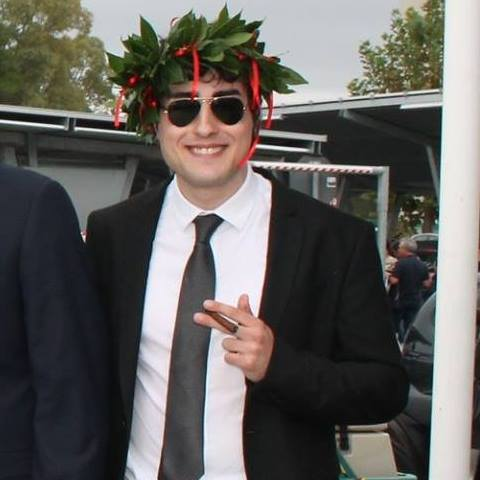
\includegraphics[width=3cm]{figures/marco.jpg}
\vspace{0.3cm}

\raisebox{-0.35ex}{
\includegraphics[width=4ex]{figures/link.png}}%
\hspace{0.05cm} /marcochiarelli

\end{figure}

\begin{figure}[h]

\includegraphics[width=3cm]{figures/gabriele.jpg}
\vspace{0.3cm}

\raisebox{-0.35ex}{
\includegraphics[width=4ex]{figures/link.png}}%
\hspace{0.05cm} /gabrieleaccarino

\end{figure}

\begin{figure}[h]

\includegraphics[width=3cm]{figures/paolo.jpg}
\vspace{0.3cm}

\raisebox{-0.35ex}{
\includegraphics[width=4ex]{figures/link.png}}%
\hspace{0.05cm} /paolo-panarese-6a016187

\end{figure}

\begin{figure}[h]

\includegraphics[width=3cm]{figures/emanuele.jpg}
\vspace{0.3cm}

\raisebox{-0.35ex}{
\includegraphics[width=4ex]{figures/link.png}}%
\hspace{0.05cm} /emanuele-costa-cesari-40ab1211a

\end{figure}


%BIBLIOGRAFIA - redatta con il relativo ambiente
\begin{thebibliography}{100}
\bibitem{rif1} G. Indiveri \emph{Notes on Rotations, Orientation Errors and Robot Kinematics}
\bibitem{rif2} G. Indiveri \emph{Introduzione alla tecnica dei Minimi Quadrati per l'identificazione parametrica e la stima dello stato}
\bibitem{rif3} G. Indiveri \emph{Ph.D Thesis, Chapter 3}
\bibitem{rif4} L. Sciavicco, B. Siciliano \emph{Robotica industriale}
\bibitem{rif5} A. Della Ducata \emph{Notazione di Denavit - Hartenberg}
\bibitem{rif6} L. Fortuna, M. Frasca \emph{Complementi di Teoria dei Sistemi e di Controlli Automatici}
\bibitem{rif7} T. I. Fossen, J. W. \& Sons \emph{Guidance and Control of Ocean Vehicles}
\bibitem{rif8} \emph{Handbook of (Marine) Robotics}
\bibitem{rif9} N. Newman \emph{Marine Hydrodynamics}
\end{thebibliography}

\end{document}


%************************************************
% Chapter 2: ROTAZIONI
%************************************************
% !TEX encoding = UTF-8
% !TEX TS-program = pdflatex
% !TEX root = ../rob.tex
% !TEX spellcheck = it-IT

%************************************************
\chapter{Rotazioni}
\label{cap:rot}
%************************************************\\

\section{Matrici di ROTAZIONE}

L'oggetto matematico che permette di descrivere la posizione di una terna rispetto ad un'altra è la matrice di ROTAZIONE.

\begin{defn}{\textbf{Matrice di ROTAZIONE}}

Dati due sistemi di riferimento $\{<0>,\ <1>\}$ indicati rispettivamente dalla seguente coppia di terne di versori mutuamente perpendicolari: $\{(i_0,j_0,k_0),\ (i_1,j_1,k_1)\}$, definiamo \textit{matrice di rotazione} tra il sistema $<0>$ ed il sistema $<1>$ (l'ordine di enunciazione delle terne è importante) il seguente oggetto matematico:

\[
	^1R_0 =
	\begin{bmatrix}^1i_0\in\R^{3\times 1}&^1j_0\in\R^{3\times 1}&^1k_0\in\R^{3\times 1}\end{bmatrix}
\]

dove, come graficamente esposto, i singoli elementi trascritti nella matrice sono dei vettori colonna. Ognuno di essi rappresenta il versore $i$-esimo, $i=1,2,3$ della terna $<0>$ espresso in terna $<1>$.

\end{defn}

Notiamo che:

\[
	\left\{
	\begin{aligned}
	&^0i_0 =  \begin{bmatrix}1&0&0\end{bmatrix}^\top\\
	&^0j_0 =  \begin{bmatrix}0&1&0\end{bmatrix}^\top\\
	&^0k_0 =  \begin{bmatrix}0&0&1\end{bmatrix}^\top
	\end{aligned}
	\right.
\]

$i_0$ è un versore. Oggetto di grandezza unitaria (in norma), il quale esiste a prescindere dalle sue componenti! I tre numeri conservano la MEMORIA in cui li ho calcolati. La matrice descrive l'assetto. Utile perché se conosco un vettore in una terna e voglio calcolare le sue componenti in terna $<1>$, è sufficiente effettuare questa operazione:

\[
	^1p =\ ^1R_0\ ^0p
\]

\`E semplicemente un prodotto matrice vettore. Ricordiamo che tale operazione è sostanzialmente una combinazione lineare degli elementi di una matrice (colonne) pesati con coefficienti forniti dal vettore con il quale si intende essa moltiplicare:

\[
	y = Mx = x_1m_1 + x_2m_2 +\ \dots\ + x_nm_n
\]

Una tale matrice di rotazione esprime l'assetto. Come è orientata la terna $<0>$ in terna $<1>$? Se prendiamo una direzione nota in terna $<0>$, e vogliamo vedere a cosa quella direzione corrisponde in terna $<1>$, è sufficiente utilizzare: $[^1p =\ ^1R_0\ ^0p]$, che corrisponderebbe alla proiezione in terna $<1>$ del vettore $^0p$. Quindi:

\[
	^1R_0 =
	\begin{bmatrix}{^1}i_0\in\R^{3\times 1}&^1j_0\in\R^{3\times 1}&^1k_0\in\R^{3\times 1}\end{bmatrix}
\]

Ovviamente, per via della disuguaglianza triangolare, ogni colonna deve sommare ad 1 in norma. Per essere una matrice di rotazione, i suoi elementi non saranno MAI maggiori di 1 in modulo! Tabellina di 9 numeri. Se li mettessimo random, molto probabilmente non otterremmo una matrice di rotazione! Ciascuna colonna ha esattamente NORMA 1! (Sono VERSORI!). Abbiamo tre $(1+1+1)$ vincoli relativi alla norma dei versori più tre altri vincoli $(1+1+1)$ relativi al fatto che, rispettivamente: $\{i\perp j,\ j\perp k,\ i\perp k\}$. Tabella di 9 numeri vincolata da 6 equazioni. Ne rimangono 3 altri gradi di libertà, pari quindi al numero di parametri minimi necessari a descrivere univocamente una matrice di rotazione. Rappresentazione minima: servono 3 numeri indipendenti (minimo) per (de)scrivere una matrice di rotazione. Come scegliere questi tre numeri è una storia abbastanza lunga. Alcuni ne scelgono 4 numeri al posto di 3 (QUATERNIONI). Altra caratteristica (tipicamente interconnessa alle altre): $^1p$ è una copia di $^0p$ MA in un altro sistema di riferimento. Ovviamente le componenti / orientazioni cambiano, ma la NORMA no! Dal punto di vista delle componenti, la NORMA di un vettore NON ha bisogno di loro! \`E semplicemente una funzione definita in maniera assiomatica, quindi una distribuzione in tal senso:

\[
	\norma{x}:\R^n\mapsto \R\ |\\
	\left\{
	\begin{aligned}
	&\norma{x} \geq 0,\ \norma{x} = 0 \iff x=0\\
	&\norma{x+y} \le \norma{x}+\norma{y}
	\end{aligned}
	\right.
\]

\`E in realtà a nostra discrezione come definirla! Se questa "turca" funzione soddisfa alle seguenti condizioni, allora è una norma! La norma euclidea è una qualsiasi norma possibile tra le tante (infinite). \`E calcolabile comodamente mediante l'utilizzo delle componenti:

\begin{corl}{\textbf{Calcolo della norma di un vettore mediante componenti}}

\[
	[\norma{x}^2 = X_x^2 + X_y^2 + X_z^2]
\]

\end{corl}

Ma anche le norme, ovviamente, prescindono anch'esse dalle componenti dei vettori. Infatti una definizione più pragmatica e rigorosa è la seguente, della quale il risultato precedente è infatti un corollario:

\begin{defn}{\textbf{Norma di un vettore}}

\[
	[\norma{p\in\R^{3\times 1}}_2 = \sqrt{p^\top p}]
\]

\end{defn}

Proviamo ad applicare la seguente definizione al vettore: $^1p$:

\[
	\norma{^1p}^2 =\ ^1p^\top\ ^1p =\ ^0p^\top\ ^1R_0^\top\ ^1R_0\ ^0p \stackrel{ISOMTRC}{=}\ ^0p^\top\ ^0p = \norma{^0p}^2
\]

Risultato che mostra che la matrice di rotazione esprime una trasformazione ISOMETRICA. Questo risultato naturalmente, wlog, vale $\forall\ ^1p$! Ciò significa che:

\begin{defn}{\textbf{Unitarietà di una matrice di rotazione}}

\[
	^1R_0^\top\ ^1R_0 = I_{3\times 3}
\]

\begin{itemize}
\item La matrice $^1R_0$ è INVERTIBILE! Ovvero ha sempre rango pieno;
\item La sua inversa concide con la TRASPOSTA. (Definizione di matrice unitaria, la quale in campo complesso indica che l'inversa coincide con la TRASPOSTA (COMPLESSA) CONIUGATA, mentre in campo reale indica proprio la definizione appena esplicitata, e si parla di matrice ORTONORMALE).
\end{itemize}

\end{defn}

Le MATRICI UNITARIE, come appena visto, sono \underline{isometriche}. Le operazioni isometriche (lineari, descritte da matrici), sono sicuramente legate a MATRICI UNITARIE. Se lo pensiamo in termini di definizione di $^1R_0$, allora il risultato è OVVIO!

\[
	^1R_0^\top\ ^1R_0 =
	\begin{bmatrix}^1i_0^\top\ ^1i_0 = 1 & 0 & 0\\0 & ^1j_0^\top\ ^1j_0 = 1 & 0\\0 & 0 & ^1k_0^\top\ ^1k_0 = 1\end{bmatrix} = I_{3\times 3}
\]

Adoperiamo ora l'applicazione del teorema di Binet sul determinante di un prodotto: per una matrice quadrata, abbiamo che il determinante della matrice prodotto è pari al prodotto dei determinanti delle singole matrici. Inoltre sappiamo che il determinante della matrice trasposta è pari al determinante della matrice in esame. Mettendo insieme ambo le cose, otteniamo:

\[
	(\det{R})^2 = 1 \implies \det{R} = \pm 1
\]

Il determinante di $R$ è quindi: $\{+1,\ -1\}$. Tutte le matrici unitarie hanno determinante di valore assoluto pari ad 1. Riassumiamo quindi i seguenti fatti:

\begin{itemize} 

\item Tutte le matrici unitarie hanno sicuramente $(\det{R})^2 = 1$;
\item Le ROTAZIONI hanno determinante della matrice di rotazione pari a $(+1)$;
\item Le RIFLESSIONI (quando ci guardiamo allo specchio es.) hanno determinante pari a $(-1)$.

\end{itemize}

Non esiste difatti una rotazione che possa eseguire il mapping relativo ad un'operazione di riflessione. Anche le RIFLESSIONI però conservano la norma, sono quindi pure loro delle isometrie. Supponiamo ora di avere: $h\in\R\ |\ \norma{h}=1$ un versore (vettore di norma unitaria). Consideriamo la seguente matrice di trasformazione:

\[
	Q = I_{3\times 3} - 2hh^\top
\]

Proviamo ad applicarla ad un vettore $v$:

\[
	Qv = (I_{3\times 3} - 2hh^\top)v = v - 2hh^\top v
\]

\begin{itemize}

\item Se $v=h \implies Q(v=h) = -h$ (il vettore $h$ semplicemente cambia segno);
\item Se $(v\perp h \iff v^\top h=h^\top v=0) \implies Qv = v$;

\end{itemize}

Supponiamo di avere un vettore $h = \begin{bmatrix}1&2&7\end{bmatrix}^\top$. Abbiamo che:

\[
	hh^\top = \begin{bmatrix}1&2&7\end{bmatrix}^\top \begin{bmatrix}1&2&7\end{bmatrix} = \begin{bmatrix}1&2&7\\2&4&14\\7&14&49\end{bmatrix}
\]

Notiamo che tale matrice è simmetrica, ma ovviamente si poteva già vedere dal fatto che: $(2hh^\top)^\top = 2hh^\top$. Calcoliamo ora:

\[
	Q^\top Q = (I-2hh^\top)^\top (I-2hh^\top) = I - 2hh^\top - 2hh^\top + 4h(h^\top h = 1)h^\top = I_{3\times 3}
\]

$Q$ è una matrice simmetrica $\impliedby Q^\top = Q$. $Q$ è un'ISOMETRIA. Questa matrice $(Q\in\R^{3\times 3})$ conserva la norma, la lunghezza. $h$ è arbitrario. Basta che sia un versore, a norma 1. NON tutte le ISOMETRIE sono delle rotazioni! Prende un vettore e cambia soltanto il segno delle componenti lungo l'asse ortogonale al piano! Questa è proprio una riflessione!

La trasformata risultante è: trasforma una terna destrorsa in una sinistrorsa. $\nexists$ modo di ruotare una terna per far diventare una terna destrorsa in una sinistrorsa. $(\det{Q}=-1)$. Non tutte le matrici ISOMETRICHE sono delle rotazioni. Esistono operazioni isometriche che non sono delle rotazioni, come appena visto.

$A^\top A = I \implies A$ ISOMETRIA. Tutte le matrici ISOMETRICHE in $\R^n$ hanno determinante della matrice associata $+1$ o $-1$. Le ROTAZIONI sono delle isometrie particolari a determinante $(+1)$.

\begin{defn}{\textbf{Gruppo delle MATRICI ORTONORMALI}}

\[
	\underline{\Theta(n)} = \{M\in\R^{n\times n}\ |\ MM^\top = M^\top M = I_{n\times n}\}
\]

\end{defn}

Prendiamo un paniere delle tali matrici appena definite. Il termine sottolineato è l'insieme delle matrici ortonormali in $\R^n$. Tale oggetto è un gruppo. Gode delle proprietà di gruppo:

\begin{itemize}

\item $\exists$ elemento unitario;
\item Il gruppo è chiuso rispetto al prodotto;
\item associatività (possiamo "spostare" le parentesi).

\end{itemize}

Con i gruppi si può astrarre, ed ottenere delle proprietà particolari per degli oggetti che siano gruppi. $\Theta(n)$ è il gruppo delle trasformazioni isometriche. Un generico elemento che vi appartiene ha determinante $\{+1,\ -1\}$. Lì dentro ci sono pure le rotazioni.

\begin{defn}{\textbf{Gruppo delle rotazioni $\SO(n)$}}

\[
	\SO(n) = \{M\in\R^{n\times n}\ |\ M^\top M = MM^\top = I_{n\times n},\ \underline{\det{M}} = +1\}
\]

\end{defn}

Sicuramente tali matrici sono delle matrici di ROTAZIONE. Matrici speciali ortonormali di ROTAZIONE in $\R^n$. \underline{MATRICI ISOMETRICHE} a determinante $(+1)$; (conservano le lunghezze). $\SO(n)$ è ANCORA UN GRUPPO! Fondamentale. Due matrici di rotazione diverse, se moltiplicate, restituiscono in output una matrice ancora appartenente al gruppo. Eredita quindi l'elemento identico di $\Theta(n)\ (I_{n\times n}\in\R^{n\times n})$. Esiste l'INVERSA, e coincide con la TRASPOSTA, dato che le matrici in gioco sono unitarie. 

Ricordiamo ora le proprietà delle trasformazione di riflessione:

\[	
	\left\{
	\begin{aligned}
	&Qh = -h\\
	&Qv = v \impliedby (v\perp h)
	\end{aligned}
	\right.
\]

Ricordiamo che: $^1p =\ ^1R_0\ ^0p$. Definiamo ora l'operazione di PROIEZIONE:

\begin{defn}{\textbf{\underline{OPERATORE PROIETTORE}}}

with: $h\in\R^{n\times n},\ \norma{h}=1$:

\[	
	M = I_{n\times n} - hh^\top
\]

\end{defn}

Con la seguente matrice prendiamo un versore in $\R^n$ (vettore di norma 1) e ne tagliamo tutte le componenti lungo $h$. Abbiamo:

\begin{itemize}

\item $Mh = 0$;
\item $M(v\perp h) = v$;

\end{itemize}

In un problema di CINEMATICA è scomodo portarsi dietro una matrice di 9 numeri. Solo 3 numeri SONO indipendenti! \`E più comodo manipolare non tutti gli elementi della matrice, ma solo i parametri MINIMI! La Scelta è però NON univoca. $\exists\infty$ modi per individuare tre parametri per descrivere una data matrice di rotazione. Bisogna introdurre una rappresentazione, la RAPPRESENTAZIONE ESPONENZIALE delle matrici di ROTAZIONE. Solo in $\R^3$ (In $SO(3)$ i suoi elementi possono essere rappresentati in tal modo).

\subsection{Matrici simmetriche / antisimmetriche} 

\begin{thrm}{\textbf{Decomposizione simmetrica/antisimmetrica di una matrice}}

\[
	[(M\in\R^{3\times 3}) = \frac{M+M^\top}{2} + \frac{M-M^\top}{2}]
\]

\end{thrm} 

\`E un risultato interessante perché il primo termine è SIMMETRICO (matrice uguale alla sua trasposta $\iff A=A^\top$), mentre è ANTISIMMETRICO il secondo (matrice uguale a MENO la sua trasposta $\iff A=-A^\top$).

Le matrici ANTISIMMETRICHE hanno una proprietà molto particolare. Mappano i vettori in tal modo:

\[
	x^\top (Ax) \stackrel{REAL}{=} (x^\top Ax)^\top \stackrel{TRANSP}{=} x^\top A^\top x \stackrel{SKEWSYMM}{=} -x^\top(Ax) = 0
\]

ove come annotato sopra l'uguale, esso vale dal momento che $(x^\top Ax)\in\R\ \forall A\in\R^{n\times n}$. Le matrici ANTISIMMETRICHE mappano il vettore ($A$ potrebbe pure non essere isometrica ovviamente) ortogonalmente ad esso. Le matrici ANTISIMMETRICHE in $\R^{n\times n}$ godono di questa particolare proprietà.

\subsection{Skew-symmetry}

Teniamo a mente la seguente:

\[	
	M\in\R^{n\times n}\ |\ M = \frac{M+M^\top}{2} + \frac{M-M^\top}{2}
\]

Posti $a,b\in\R,\ c=a\times b \leftarrow$ (operazione lineare). 

\[
	c\mapsto \begin{vmatrix}i&j&k\\a_1&a_2&a_3\\b_1&b_2&b_3\end{vmatrix} = \underline{i}(a_2b_3 - a_3b_2) - \underline{j}(a_1b_3 - a_3b_1) + \underline{k}(a_1b_2 - a_2b_1)
\]

Gli elementi di quella matrice sono associati a componenti del vettore. Abbiamo:

\[
	S(\underline{a}\in\R^{3\times 1})\in\R^{3\times 3}
\]

Matrice $\R^{3\times 3} \ni S(\underline{a})$ che rappresenta l'operazione di prodotto vettore (se opportunamente moltiplicato per un altro vettore, opportuno). Matrice ANTISIMMETRICA. $\underline{a}$ si chiama anche VETTORE ASSIALE della matrice ANTISIMMETRICA. Qualsiasi matrice antisimmetrica ha associato un UNICO vettore assiale. Il modo banale di vederlo è che, prendendo una qualsiasi matrice random, estraendone la parte antisimmetrica $(\frac{M-M^\top}{2})$, ha sempre 0 sulla diagonale principale. Scegliendo a caso $\{a_1,\ a_2,\ a_3\}$, allora abbiamo quindi la corrispondenza: VETTORE ASSIALE $\leftrightarrow$ MATRICE ANTISIMMETRICA. Quei 3 numeri li interpretiamo come componenti del vettore assiale associato. Dimostrazione sulle dispense più efficiente (non passa per le componenti). In realtà un OPERATORE LINEARE prescinde anch'esso dalle componenti! Ha delle particolari proprietà. La dimostrazione si può fare senza fare uso delle componenti! Il prodotto vettore in $\R^3$ definisce un unico vettore assiale di una matrice antisimmetrica (e viceversa). Il risultato di $Ax$ è esprimibile mediante prodotto vettore, e viceversa:

\begin{thrm}{\textbf{Skew-symmetry Matrix and Axial Vector Mapping}}

\[
	\left\{
	\begin{aligned}
	&Ax = a\times x\\
	&a,x\in\R^{3\times 1}\\
	&(A=-A^\top)\in\R^{3\times 3}
	\end{aligned}
	\right.
\]

\end{thrm}

Dimostrazione costruttiva, senza componenti. Obiettivo: Dimostrare che $A$ è ANTISIMMETRICA: $\exists! \underline{a}\ |\ Ax=\underline{a}\times \underline{x}$. Utilizzando le componenti è abbastanza banale, già dimostrato.

\begin{proof}

\[
	\underline{a} = \frac{1}{2}\sum_{i=1}^3{e_i\times Ae_i} = (\dots)
\]

Bisogna applicare le proprietà del prodotto vettore, e ad un certo punto ovviamente la proprietà di antisimmetria per $A$. Chiamiamo con $e_i$ il generico versore $i$-esimo dello spazio $\R^3$ (individuiamo una base ortonormale arbitraria di $\R^3$). Segue:

\[
	\underline{a}\times\underline{x} = \underline{\frac{1}{2}[\sum_{i=1}^3{(e_i\times Ae_i)]}}\times\underline{x} = \frac{1}{2}\sum_{i=1}^3{(\underline{x}\times(Ae_i\times e_i))} = (\dots)
\]

Ove abbiamo cambiato l'ordine del prodotto vettore due volte onde evitare il segno. Si rammenti la regola del TRIPLO PRODOTTO:

\[
	a\times(b\times c) = b(a^\top c) - c(a^\top b)
\]

Sempre vera. L'ordine nel prodotto vettore conta! Si effettui prima $(b\times c)$, e lo si moltiplichi secondo prodotto vettore per $\underline{a}$. Quindi, tornando a noi:

\[
	(\dots) = \frac{1}{2}\sum_i{[\underline{(Ae_i)(x^\top e_i)} - e_i(x^\top Ae_i)]} = (\dots)
\]

Ove il termine sottolineato sommato ad $i$ restituisce proprio $Ax$, per definizione. Ora applichiamo l'antisimmetria.. se anziché $x^\top Ae_i$ ne mettessimo la versione invertita, allora esso cambierebbe segno. Fino ad ora abbiamo fatto semplicemente del calcolo generico.

\[
	(\dots) \stackrel{SKEWSYMM}{=} [\frac{1}{2}(Ax + \underline{\sum_i{e_i((Ax)^\top e_i)}}] = \frac{Ax}{2}+\frac{Ax}{2} = Ax
\]

\end{proof}

Ove il termine sottolineato è sempre $Ax$. Ciò chiude la dimostrazione. Questo vettore assiale $\underline{a}$ è UNICO! Dimostrazione semplice per esercizio. Non è molto standard, ma l'operazione che mappa una matrice antisimmetrica nel suo vettore assiale è la seguente, definita mediante il seguente mapping:

\[
	\Vex(A) = \underline{a}\in\R^{3\times 1}
\]

Abbastanza pesante come notazione, ma non infrequente in letteratura. Pseudo-vettore in realtà. Nell'ambito delle rotazioni il vettore assiale lo incontreremo abbastanza di frequente. $\underline{a}=\begin{bmatrix}a_1&a_2&a_3\end{bmatrix}^\top$. La matrice $A$, è quindi:

\[
	A := S(\Vex(A)) = S(\underline{a}) =
	\begin{bmatrix}0&-a_3&a_2\\a_3&0&-a_1\\-a_2&a_1&0\end{bmatrix}
\]

Se una tale matrice $A$ fosse ad esempio: $A:=\begin{bmatrix}0&3&2\\-3&0&-1\\-2&+1&0\end{bmatrix}$, allora il suo vettore assiale sarebbe: $Vex(A):=\underline{a}=\begin{bmatrix}1&2&-3\end{bmatrix}^\top$. Sul segno vi è in realtà un po' di ambiguità, ma non relativamente al vettore assiale in sé per sé.

La regola del triplo prodotto è stata molto utile, e sarà tale ancora durante il prosieguo del corso:

\begin{thrm}{\textbf{Regola del TRIPLO PRODOTTO}}

\[
	\underline{a}\times(\underline{b}\times\underline{c}) = \underline{b}(a^\top c) - \underline{c}(a^\top b) = (\dots)
\]

\end{thrm}

Questo fatto mette in evidenza che questa operazione tra vettori, ne freeza due e tratta il terzo come parametro (costante); l'operazione è quindi lineare. Banale dimostrarlo:

\[
	[(\dots) = (I_{3\times 3}(a^\top c) -\underline{c}\underline{a}^\top \in\R^{3\times 3})\underline{b}]\in\R^{3\times 1} = (\dots)\\
\]

Rispetto $\underline{b}$ lo posso scrivere come matice per $\underline{b}$. Se fossero $\underline{a}$, o $\underline{c}$ liberi, avremmo:

\[
	\left\{
	\begin{aligned}
	&(\dots);\\
	&(\dots) = (\underline{b}\underline{c}^\top -\underline{c}\underline{b}^\top)\underline{a};\\
	&(\dots) = [\underline{b}\underline{a}^\top -I_{3\times 3}(\underline{a}^\top\underline{b})]\underline{c};
	\end{aligned}
	\right.
\]

Operatore lineare su uno dei tre argomenti. Su qualche passaggio cinematico tornerà utile. Regola del triplo prodotto banalmente dimostrabile per calcolo diretto. Mostriamo un po' di \emph{sugar calculus}:

\[
	\left\{
	\begin{aligned}
	&\{\Vex(A),\ \underline{S^\top(\underline{a}) = -S(\underline{a})}\}\\
	&[\Vex(A)=\underline{a} \implies \Vex[S(\underline{a})] = \underline{a}]
	\end{aligned}
	\right.
\]

\subsubsection{Proprietà di una Matrice Antisimmetrica}

\`E utile sapere che la potenze di una matrice antisimmetrica hanno una particolare ricorsione. Calcolabile di nuovo per calcolo diretto:

\[	
	\{S(\underline{a})S(\underline{a}) := S^2(\underline{a}),\ S(\underline{a})S(\underline{a})S(\underline{a}) := S(\underline{a})^3,\ \dots\}
\]

Ad occhio vengono fornite le seguenti formule. Dato: $\underline{h}\in\R^{3\times 1}\ |\ \norma{h}=1$ VERSORE, abbiamo:

\[
	\left\{
	\begin{aligned}
	&S(\underline{h}) = \underline{h}\times\mathord{\cdot}\\
	&S^2(\underline{h}) = hh^\top - I_{3\times 3}\\
	&S^3(\underline{h}) = -S(\underline{h})\\
	&S^4(\underline{h}) = -S^2(\underline{h})
	\end{aligned}
	\right.
\]

Possiamo generalizzare:

\begin{thrm}{\textbf{Potenze di una MATRICE ANTISIMMETRICA}}

\[
	\left\{
	\begin{aligned}
	&S^{2i+1}(\underline{h}) = (-1)^iS(\underline{h})\\
	&S^{2(i+1)}(\underline{h}) = (-1)^i(\underline{hh^\top -I_{3\times 3}})
	\end{aligned}
	\right.
\]

\end{thrm}

Ricordiamo che $(I_{3\times 3} - hh^\top)$ è il proiettore. Quindi il termine sottolineato è il proiettore cambiato di segno. Per alcune potenze pari (precisamente le potenze pari di esponente $i$ dispari), sarà proprio il proiettore, per le altre sarà il proiettore cambiato di segno, per l'appunto.

$S(\underline{h})v=h\times v,\ \Tr(S(\underline{h})=0)$. La traccia delle potenze dispari continuerà quindi ad essere 0. La traccia delle potenze pari, data la traccia particolare che $hh^\top$ esibisce ovvero $\Tr(hh^\top) = h^\top h=1$, ha la seguente espressione:

\[
	[\Tr(S^{2(i+1)}(\underline{h})) = (-1)^{i+1}2]
\]

Ulteriore proprietà: stupidaggine ma fino ad un certo punto: verrà comoda più in avanti. \`E la seguente: $\forall$ matrice antisimmetrica $\mathord{\cdot}\in\{\R^{3\times 3}\}$ è associato un UNICO VETTORE ASSIALE!

Ora prendiamo $\{\exists M\in\R^{3\times 3},\ \underline{x}\in\R^{3\times 1}\}$.
Eventualmente $M$ può anche essere a simmetria non ben definita. Calcoliamo la trasposta della matrice ottenuta a valle dell'applicazione della trasformazione di similitudine:

\[
	(M\underline{S(\underline{x})}M^\top)^\top = MS(\underline{x})^\top M^\top = -MS(\underline{x})M^\top
\]

$\implies [MS(\underline{x})M^\top]$ antisimmetrica! Essendo antisimmetrica, deve ammettere un vettore assiale: 

\begin{thrm}{\textbf{Trasformazione di similitudine di una Matrice Antisimmetrica}}

\[
	\left\{
	\begin{aligned}
	&MS(\underline{x})M^\top = S(\underline{y})\\
	&y = (L\in\R^{3\times 3})x
	\end{aligned}
	\right.
\]

\end{thrm}

$(L\in\R^{3\times 3})$ è stata già calcolata. Usiamo la notazione \emph{MATLAB}, ove $M(2,:)$ indica la seconda riga (quindi in versione trasposta rappresenterebbe un vettore colonna); ad esempio il termine citato prima corrisponde alla riga selezionata della matrice $M$ così parametrizzata:

\[
	\begin{bmatrix}m_{11}&m_{12}&m_{13}\\\underline{m_{21}}&\underline{m_{22}}&\underline{m_{23}}\\m_{31}&m_{32}&m_{33}\end{bmatrix}
\]

abbiamo:

\[
	L = \begin{bmatrix}\begin{bmatrix}M(2,:)^\top\times M(3,:)^\top\end{bmatrix}^\top\\\begin{bmatrix}M(3,:)^\top\times M(1,:)^\top\end{bmatrix}^\top\\\begin{bmatrix}M(1,:)^\top\times M(2,:)^\top\end{bmatrix}^\top\end{bmatrix}
\]

$M$ è la più generale possibile. Se prendiamo per $M$ un elemento di $\SO(3)$ (matrice di rotazione), la $L$ associata è proprio $M$! Ovvero la tale matrice di rotazione scelta. A valle dell'analisi, del tutto generale, ricaviamo un utilissimo risultato particolare. Prendiamo una generica matrice di rotazione:

\begin{corl}{\textbf{Trasformazione di similitudine di una Matrice Antisimmetrica}}

$R\in\SO(3),\ \forall x\in\R^{3\times 1}$:

\[
	[RS(\underline{x})R^\top = S(Rx)]
\]

\end{corl}

\`E un risultato abbastanza semplice. Dal punto di vista algebrico è come abbiamo detto prima. In $\SO(3),\ L=R$. Un interpretazione geometrica è molto profonda. Una rotazione, dal punto di vista geometrico, è un'ISOMETRIA (che CONSERVA le distanze), che conserva il PRODOTTO VETTORE. Le rotazioni fanno sì che le distanze relative tra due punti fissi rimangano uguali! Trasformazione di similitudine:

\[
	\underline{RS(\underline{x})R^\top = S(R\underline{x})}
\]

$\leftarrow$ le rotazioni conservano il prodotto vettore: ruotando il risultato del prodotto vettore è la stessa cosa del ruotare singolarmente, isolatamente l'operando sinistro di esso (del prodotto vettore). \`E un risultato in realtà abbastanza potente!

Possiamo adesso analizzare un legame profondo e significativo tra gli elementi di $\SO(3)$ e le \underline{matrici esponenziali}:

\subsection{Matrici ESPONENZIALI}

\begin{defn}{\textbf{Matrice ESPONENZIALE}}

$M\in\R^{n\times n}\ \theta\in\R,\ \forall i,j$

\[
	(L = \e^{M\theta}\in\R^{n\times n}) := (\underline{\sum_{l=0}^{+\infty}{\frac{M^l\theta^l}{l!}}}) < +\infty \iff e^{M\theta}_{ij} <+\infty
\]

\end{defn}

Tale matrice è nientemeno che la matrice $e^{At}$ vista in TdS. $\e$ è proprio il simbolo di Nepero in tal caso, ma stavolta rappresenta una matrice intesa come autofunzione rispetto ad operatori differenziali, come vedremo dalle prossime proprietà.
La sommatoria tra parentesi tonde CONVERGE sicuramente! La sommatoria rappresenta infinite potenze, scalate per $\frac{1}{l!}$ e sommate. Converge ad una quantità finita, ovvero in tal caso ad una matrice con elementi tutti finiti. Come già anticipato, il motivo per cui utilizziamo questa notazione è che, non solo ricorda Taylor, ma questa matrice qui gode di parecchie proprietà, molte delle quali analoghe a quelle dell'esponenziale scalare.

\subsubsection{Proprietà della Matrice Esponenziale}

Dal punto di vista concettuale le seguenti proprietà sono molto profonde:

\begin{itemize}

\item La matrice $\e^{M\theta}$ è sempre INVERTIBILE, $\forall M$ anche NON INVERTIBILE!
\item Al posto di $M$, mettendovi $-M$, ed eseguendo l'esponenziale matriciale otteniamo l'inversa di $(\e^{M\theta})$:
$\inv{(\e^{M\theta})} = \e^{-M\theta}$;
\item $(\e^{M\theta})^\top = \e^{M^\top\theta}$;
\item $[\underline{M\e^{M\theta} = \e^{M\theta}M}]$.

\end{itemize}

Le matrici generiche tra di loro non commutano generalmente rispetto al prodotto matriciale. L'ultima proprietà è un risultato abbastanza stupido: si ottiene semplicemente moltiplicando per $M$ ambo i membri della definizione, e vedendo cosa si ottiene nell'RHS..

La matrice non è tuttavia banale da calcolare generalmente. Una delle sue possibili difficoltà è che le potenze non hanno una struttura semplice o ben definita. Ci sono alcuni casi invece semplici e banali, ad esempio nel caso di matrici $M$ NILPOTENTI (dopo alcune potenze diventano 0) oppure IDEMPOTENTI. Se è diagonalizzabile ci sono invece altri trucchi, legati alla costruzione delle cosiddette matrici di JORDAN, LAPLACE, etc.. Se $l=17$, abbiamo 17 termini nella sommatoria matriciale.

Notazioni matematiche: $\{\{h\in\R^{3\times 1},\ \norma{h}=1\},\ SCALAR\ \theta\in\R\}$. Calcolando:

\[
	[\underline{\e^{\theta S(\underline{h})} \in\R^{3\times 3}}] \in\SO(3)
\]

Vi è un legame SURGETTIVO sostanzialmente. Vale un risultato fondamentale, dimostrato da Eulero nel 1700. Possiamo ricoprire tutto $\SO(3)$. $\forall$ elemento di $\SO(3)$, ammette tanti $\theta,\ \underline{h}$ tale per cui valga l'appartenenza al gruppo prima esplicitata. La ricopertura è addirittura troppo buona! Nel senso che, vi sono diversi modi (parametri) per giungere allo stesso elemento di $\SO(3)$, come vedremo più in avanti.

\subsubsection{Rappresentazione esponenziale delle Matrici di Rotazione}

Tale sottosezione è di una notevole importanza pratica! Praticamente ENORME! Non solo dal punto di vista teorico. Tale formula tuttavia non ci dice ancora niente. Proprio perché la matrice esponenziale è difficile da calcolare $(\e^{\theta S(\underline{h})})$. In realtà quella formula si può semplificare (RODRIGUES). Dobbiamo dimostrare anzitutto che:

\begin{thrm}{\textbf{Appartenenza ad $\SO(3)$ delle Matrici Esponenziali (Speciali)}}

\[
	[\e^{\theta S(\underline{h})}\in\SO(3)]
\]

\end{thrm}

\begin{proof}


\begin{itemize}

\item{\textit{Unitarietà della matrice}}:

\[
	(\e^{\theta S(\underline{h})})^\top(\e^{\theta S(\underline{h})}) \stackrel{EXP}{=} \e^{\theta S^\top(\underline{h})}\e^{\theta S(\underline{h})} = (\dots)
\]
\[
	(\dots) = \e^{\theta (S^\top(\underline{h}) + S(\underline{h}))} = \stackrel{SKEWSYMM}{=} \e^{\theta(-S(\underline{h})+S(\underline{h}))} \stackrel{EXPINV}{=} I_{3\times 3}
\]

\item{\textit{Determinante positivo unitario}}:

Abbiamo anche dimostraro che, per Binet, il determinante al quadrato è 1! $(\det(\e^{\theta S(\underline{h})}) = \pm 1)\ \forall\theta\forall h$! Come facciamo a dimostrare che è proprio $+1$ e non $-1$? Il determinante di una matrice è una funzione continua dei suoi elementi. Se sapessimo scrivere $(\e^{\theta S(\underline{h})})$ (i suoi singoli elementi), ci aspetteremmo che essa sia una funzione di 4 numeri, di 4 parametri: $(\begin{bmatrix}h_1&h_2&h_3\end{bmatrix}^\top, \theta)$. Il determinante sarà o costantemente $+1$, o costantemente $-1$. \`E una funzione continua dei suoi parametri. Se prendiamo $(\theta=0)$, abbiamo:

\[
	(\e^{0S(\underline{h})} = I_{3\times 3})
\]

il cui determinante è proprio $(+1)$! In un punto quindi il determinante lo sappiamo calcolare, e lo abbiamo calcolato in maniera esatta. $+1$ ovunque. Relativamente sottile come ragionamento, ma non difficile. Tale risultato, ricapitolando, si ottiene mettendo insieme due cose:

\begin{itemize}

\item Determinante in modulo unitario;
\item Determinante funzione continua degli elementi della matrice.

\end{itemize}

\end{itemize}

\end{proof}

In questa definizione non abbiamo supposto che $h$ fosse un VERSORE. VETTORE GENERICO. Per comodità (wlog), si utilizzerà $h\ |\ \norma{h}=1$.

\subsubsection{Formula di Rodrigues}

Se prendiamo la formula dell'esponenziale matriciale, riscrivendola:

\[
	[\e^{\theta S(\underline{h})} \in\SO(3)]
\]

Mi ricordo della definizione di matrice esponenziale. La riscrivo computandola per esteso, trovando:

\begin{defn}{\textbf{FORMULA DI RODRIGUES}}

\[
	\e^{\theta S(\underline{h})} = I_{3\times 3} + \sum_{l=1}^{+\infty}{\frac{S^l(\underline{h})}{l!}\theta^l} \stackrel{REC.SKEWPOWER}{=} (\dots)
\]
\[
	(\dots) = [I_{3\times 3} + \sin(\theta) S(\underline{h}) + (1-\cos(\theta))S^2(\underline{h})]
\]

\end{defn}

ove si è utilizzato nell'ultimo passaggio della definizione le formule delle potenze di $S(\underline{h})$, trovando il risultato esposto per semplice pura ispezione visiva.

A questo punto la matrice di rotazione la riusciremo a scrivere! Con carta e penna, MATLAB, C, Java, etc. Ad esempio: $\{h\ VERSORE\ |\ \norma{h}=1\},\ \theta=35^{\circ}$. Disponendo quindi dei seguenti elementi: $\{h,\theta\} \leftrightarrow$ \{versore dell'asse, angolo di rotazione\}, riusciamo quindi a scrivere la matrice di rotazione. La formula di Rodrigues è stata quindi ottenuta dal riconoscimento dello sviluppo in serie di Taylor delle funzioni trigonometriche applicato alla scrittura delle varie potenze della matrice antisimmetrica. Va detto che $h$ è il versore dell'asse di rotazione. Dev'essere un autovettore di $R$ con autovalore associato $1$, dal momento che abbiamo la seguente direzione preferenziale:

\[
	(\e^{\theta S(\underline{h})}\underline{h}) = \underline{h}
\]

$h$ è quindi la direzione dell'asse di rotazione. $\theta$ dev'essere necessariamente l'angolo. Ci rimane da chiederci: se prendo un generico elemento di $\SO(3)$, $\exists h\in\R^{3\times 1}\ |\ \norma{h}=1,\ \theta\in\R$ tale per cui esista una matrice esponenziale $\e^{\theta S(\underline{h})}$ che lo rappresenti? Ruotare di $(\theta=0^{\circ})$ vuol dire avere infiniti $h$ (qualsiasi asse possibile). Per scrivere problemi di controllo, ad esempio l'orientazione di un satellite, mi calcolo dei parametri delle posizioni finali. Mi calcolo la \underline{fdt $h(t)$} (se fosse lineare), la quale avrebbe matematicamente una SINGOLARIT\`A. \`E un problema di Rappresentazione, NON problema fisico. Le Rappresentazioni esponenziali delle matrici di rotazione hanno questi problemi (NON-UNIVOCIT\`A, ovvero SINGOLARIT\`A in gioco).

\subsubsection{Mapping SURGETTIVO}

Abbiamo un mapping surgettivo tra la matrice exp e gli elementi in $\SO(3)$. Ricordiamo che:

\[
	\e^{S(\underline{h})\theta} = I_{3\times 3} + \sin(\theta)S(\underline{h}) + (1-\cos(\theta))S^2(\underline{h})
\]

con $\underline{h}\in\R^{3\times 1},\ \norma{h}=1,\ \theta\in\R$. La sopracitata formula di Rodrigues vale $\forall\theta\forall \underline{h}$. Il problema è notare che esistono infiniti $\theta$ e $\underline{h}$ che consentono di individuare elementi in $\SO(3)$. Notiamo che scelto $(\theta\in\R)$, si potrebbe ottenere la stessa matrice exp andando a scalare $\theta$ di un fattore $2k\pi$, giacché le funzioni trigonometriche in gioco sono periodiche di periodo $2\pi$. NB: Il legame tra l'evoluzione temporale di un matrice di rotazione ed i suoi parametri $\{\underline{h},\ \theta\}$ che la descrivono non è banale! Occorre definire il fattore integrante: il vettore velocità angolare. Occorre focalizzarsi sulla posa iniziale e quella finale, ma non si hanno gli strumenti per descrivere la traiettoria.

Ogni matrice quadrata $n\times n$ è decomponibile nella somma di una parte simmetrica e di una antisimmetrica, e questo si evince anche nella formula di Rodrigues. Data una matrice arbitraria $R\in\SO(3)$, abbiamo:

\[
	[\Vex(\frac{R-R^\top}{2}) = \sin(\theta)\underline{h}]
\]

Se calcoliamo la traccia di $\e^{S(\underline{h})\theta}$, noteremo che la parte antisimmetrica non dovrebbe contribuire, dal momento che tale matrice ha tutti 0 sulla diagonale principale.

\[
	\left\{
	\begin{aligned}
	&S^2(\underline{h}) = hh^\top - I_{3\times 3}\\
	&\Tr(S^2(\underline{h})) = -2
	\end{aligned}
	\right.
\]

Eguagliamo ora la traccia di $R$ con quella di $\e^{\theta S(\underline{h})}$:

\[
	\Tr(R) = 3 + 0 -2(1-\cos(\theta)) = 1+2\cos(\theta) \implies
	\left\{
	\begin{aligned}
	&\centernot{2}cos(\theta) = \frac{tr(R)-1}{2}\\
	&\theta h = \frac{\theta}{\sin(\theta)} \Vex(\frac{R-R^\top}{2})
	\end{aligned}
	\right.
\]

Ma la prima equazione del sistema non è $\theta$! Dobbiamo quindi estrarre l'arcocoseno; ma quando lo estraiamo, il modulo è ben definito, ma non il segno! Il problema è che se $\theta=0$, sostituito nella seconda equazione fornisce:

\[
	\Vex(\frac{R-R^\top}{2}) = \sin(\theta)\underline{h} = 0 \implies [R=I]
\]

Non riesco quindi ad individuare un $\underline{h}$ univoco, infatti esso può essere qualsiasi con $\theta=0^{\circ}$! ($\exists\ MUL\ \underline{h}$). L'ambiguità sta in come trattiamo i parametri che sono 4: $\{h_x,\ h_y,\ h_z,\ \theta\}$. Infatti le componenti di $h$ sono dipendenti per la condizione di NORMALIZZAZIONE $\iff \norma{h}=1$; $\underline{h}$ ha due componenti linearmente indipendenti. $\underline{h}$ è un versore, le sue componenti sono scalari, e sono peraltro DIPENDENTI TRA DI LORO! Possiamo inoltre considerare un vettore:

\begin{defn}{\textbf{VETTORE ASSE-ANGOLO EQUIVALENTE}}

\[
	\nu:=\begin{bmatrix}\underline{h}^\top&\theta\end{bmatrix}^\top
\]

Tali sue quattro componenti, con $\norma{h}=1$ risultano essere equivalenti a tre variabili indipendenti. Le prime tre sono quelle di $\underline{h}$, e la quarta è $\theta$.

\end{defn}

Data $R\in\SO(3)$, possiamo calcolare il $\theta$, estraendo direttamente il coseno; Purché $\theta\neq k\pi$ possiamo direttamente calcolare $\theta\underline{h}$:

\begin{defn}{\textbf{Rotation Vector}}

\[
	[\theta\underline{h} = \frac{\theta}{\sin(\theta)}\Vex(\frac{R-R^\top}{2})]
\]

\end{defn}

where $\theta\in(-\pi,+\pi)$. Se abbiamo una rotazione di un multiplo di $\pi$, non abbiamo un solo $\theta\underline{h}$ che definisce univocamente la rotazione. La singolarità quindi non sta in 0, ma in $\pi$, dal momento che la funzione reciproca del $\sinc{\mathord{\cdot}}$ è ben definita in 0 e vale 1.


\begin{defn}{\textbf{Rappresentazioni minime in $\SO(3)$}}

Si chiamano RAPPRESENTAZIONI MINIME in $\SO(3)$ qualsiasi funzione che associa a tre valori indipendenti un elemento in $\SO(3)$. Qualunque essa sia avrà almeno una singolarità.

\end{defn}

In questi casi stiamo considerando delle situazioni in cui una terna di riferimento (es. spigoli del muro) descrive come un oggetto è orientato nello spazio. $\underline{h}$ è l'asse di rotazione: mi dice la direzione attorno alla quale ruoto di $\theta[^{\circ}]$ rispetto al S.R. correntemente in uso.

Eulero afferma che l'assetto finale dell'oggetto poteva essere raggiunto attraverso \newline\underline{UNA SOLA ROTAZIONE}! Rotazione elementare rispetto ad un particolare asse fisso, opportunamente scalato ed orientato secondo un angolo $\theta$; eventualmente anche una traslazione se l'oggetto finale si è mosso. Questa è una caratteristica intrinseca dello spazio euclideo.

Per descrivere un elemento di $\SO(3)$, possiamo utilizzare alternativamente al vettore asse-angolo equivalente altri due angoli: angoli di Eulero ed angoli di Yaw, Pitch e Roll, che sono in realtà \underline{alberi} (TREE) di angoli.

\subsection{Angoli di Eulero, YPR}

\subsubsection{Angoli di Yaw, Pitch e Roll}

L'obiettivo è trovare tre parametri in grado di descrivere un elemento di $\SO(3)$. Possiamo immaginare di usare come parametri gli angoli di rotazione utilizzati per arrivare dalla terna di partenza a quella di arrivo: gli angoli sono linearmente indipendenti, ma devo decidere se misurare la rotazione tutta rispetto a quella \underline{di partenza} (\textit{initial axis}), oppure rispetto a quella \underline{corrente} (\textit{current axis}) (quella nuova), cioè gli assi istantanei. Inoltre le rotazioni finite non contano, ma solo quelle infinitesime. Ricordiamo che:

\[
	\left\{
	\begin{aligned}
	&\begin{bmatrix}X=30^{\circ}&Y=45^{\circ}&Z=0^{\circ}\end{bmatrix}^\top\\
	&\begin{bmatrix}X=45^{\circ}&Y=30^{\circ}&Z=0^{\circ}\end{bmatrix}^\top
	\end{aligned}
	\right.
\]

non descrivono la stessa rotazione! Quindi essi \underline{NON COMMUTANO}! Occorre quindi decidere opportunamente in anticipo l'ordine della sequenza degli angoli $X,Y,Z$, oppure $Y,X,Z$, etc. Se facessimo tre rotazioni indipendenti attorno agli assi principali della terna corrente, parliamo di angoli di Yaw, Pitch e Roll.

Parliamo di angoli di Eulero quando le rotazioni avvengono attorno a sempre a due assi correnti indipendenti. Ad esempio: $\left\{\begin{aligned}&xyx\\&xzx\\&yzy\end{aligned}\right.$. Tutte queste rotazioni atomiche attorno l'asse corrente sono indipendenti purché l'angolo di rotazione dell'asse centrale sia diverso da 0. NB: Non basta dire che YAW è un angolo di rotazione rispetto a $z$, ma a seconda di come metto insieme tutte le rotazioni atomiche possiamo ottenere differenti matrici di rotazione risultanti. Entrambe le famiglie di angoli hanno almeno una singolarità, legata alla dipendenza della rotazione intorno agli assi. Le singolarità devono essere messe tipicamente a $-90^{\circ}$ (pitch), cioè lontane dall'area di lavoro; questo può essere fatto scegliendo opportunamente la sequenza di angoli.

Le rotazioni attorno gli assi $(x,y,z)$ possono finalmente essere rappresentate matematicamente.

\subsection{QUATERNIONI}

Sono vettori di quattro componenti che possono essere utilizzati per aggirare le singolarità di rappresentazione: è singolare il legame tra la matrice di rotazione e gli angoli YPR. Quando un oggetto precipita la sua matrice di rotazione è ben definita, ma non i suoi parametri che dovrebbero identificarla! Quindi se utilizzassi delle matrici non si porrebbe il problema. Il problema delle singolarità è sostanzialmente intrinseco in $\SO(3)$, quindi non c'è speranza di individuare tre parametri che non hanno singolarità di rappresentazione. Allora ne uso quattro! Così non abbiamo problemi. Definiamo:

\[
	\left\{
	\begin{aligned}
	&\mu := \cos(\frac{\theta}{2})\\
	&\underline{\epsilon} := \sin(\frac{\theta}{2})\underline{h}
	\end{aligned}
	\right.
\]

Posta la seguente condizione di NORMALIZZAZIONE: $\mu^2 + \norma{\epsilon}^2 = 1$.
Il primo termine $(\mu\in\R)$ è uno scalare, ed è la parte scalare o reale dei quaternioni, mentre $\epsilon$ è la parte vettoriale od ipercomplessa dei quaternioni. Viene posta la seguente condizione di NORMALIZZAZIONE: $\mu^2 + \norma{\epsilon}^2 = 1$. La ben nota formula di Rodrigues può essere riscritta in termini di $\{\mu,\ \epsilon\}$:

\begin{thrm}{\textbf{Formula di Rodrigues per i QUATERNIONI UNITARI}}

\[
	[R = I_{3\times 3} + 2\mu S(\underline{\epsilon}) + 2S^2(\underline{\epsilon})]
\]

\end{thrm}

\begin{proof}

\[
	R=I_{3\times 3} + \sin(\theta)S(\underline{h}) + (1-\cos(\theta))S^2(\underline{h}) = I_{3\times 3} + 2\sin(\frac{\theta}{2})\cos(\frac{\theta}{2})S(\underline{h}) + 2\sin^2(\frac{\theta}{2})S^2(\underline{h}) = (\dots)
\]
\[
	(\dots) = I_{3\times 3} + 2\mu S(\underline{\epsilon}) + 2S^2(\underline{\epsilon})
\]

\end{proof}

\underline{Non ci sono singolarità}!! In tal caso non considero il vettore $\theta\underline{h}$ (asse-angolo equivalente), ma $\epsilon$! Di conseguenza non abbiamo singolarità né in $\theta=0$ né in $\theta=k\pi$. Infatti:

\[
	\left\{
	\begin{aligned}
	&\{\mu=1,\ \underline{\epsilon}=\underline{0}\},\ \theta=0\\
	&\{\mu=0,\ \underline{\epsilon}=\underline{h}\},\ \theta=\pi
	\end{aligned} 
	\right.
\]

Ogni parametrizzazione minima cioè a tre componenti avrebbe di fatto ALMENO una singolarità.

\subsection{CINEMATICA}

Fino ad ora abbiamo parlato di \underline{rappresentazioni statiche} di terne che ruotano. Quando parliamo di rotazioni qual è l'oggetto che consente di modellare il moto nel tempo? Non sono sufficienti gli angoli di Eulero; a questo scopo viene utilizzato il vettore \underline{velocità angolare}. Sappiamo che $\forall R\in\SO(3),\ RR^\top = I_{3\times 3}$. Cio infatti segue proprio dalla membership definition degli elementi di $\SO(3)$.

\[	
	\forall R\in\SO(3),\ RR^\top = I_{3\times 3} \implies \frac{d}{dt}({^0}R_1\ ^0R_1^\top) = 0 \implies\ ^0\dot{R}_1\ ^0R_1^\top +\ ^0R_1\ ^0\dot{R}_1^\top = 0 \implies
\]
\[
	\implies [{^0}\dot{R}_1\ ^0R_1^\top = -{^0}R_1\ ^0\dot{R}_1^\top = -({^0}\dot{R}_1\ ^0R_1^\top)^\top]
\]

$R$ è sempre una qualsiasi matrice in $\SO(3)$, essa cambia nel tempo $\iff R := R(t)$, in modo tale che $RR^\top=I_{3\times 3}$, ma $^0\dot{R}_1\ ^0R_1^\top$ è \underline{antisimmetrica}. Ma ogni matrice antisimmetrica $3\times 3$ ammette vettore assiale (UNICO peraltro). Quindi:

\begin{defn}{\textbf{Vettore velocità angolare}}

$\exists!\ ^0\omega_{1/0},\ \exists\mu\in\R^{3\times 1}\ |$
\[
	[({^0}\dot{R}_1\ ^0R_1^\top)\ ^0\mu =\ ^0\omega_{1/0}\times\ ^0\mu] \implies \dot{R}R^\top = S(\omega)
\]

\end{defn}

La suddetta equazione è in realtà un'equazione differenziale! Il calcolo dell'assetto successivo $(R)$ necessita di avere $\omega$, infatti solo attraverso l'integrazione di $\dot{R}R^\top$ potremmo ottenere $R$: sarebbe sbagliato interpretare solo $\dot{R}$ come fattore integrante: otterremmo difatti un elemento non in $\SO(3)$.
$\omega$ è detto \underline{fattore integrante}, e non può essere definito tramite derivate di angoli, ma solo in maniera assiomatica attraverso il $\Vex(\mathord{\cdot})$!

\subsection{VETTORE VELOCIT\`A ANGOLARE}

Cinematica delle Rotazioni. Definizione del vettore velocità angolare:

\[
	\left\{
	\begin{aligned}
	&R\in\SO(3)\\
	&\dot{R}R^\top = S(\omega)
	\end{aligned}
	\right.\implies [\Vex(\dot{R}R^\top) :=\ ^0\omega_{1/0}]
\]

$\dot{R}R^\top\in\R^{3\times 3}$ è antisimmetrica. Quindi $\exists! \Vex(\dot{R}R^\top)$ tale che faccia valere le precedenti relazioni. Tale è il vettore velocità angolare. Etichetta $a/b$. Etichetta che la matrice $R$ mappa due terne $<A>$ e $<B>$ tramite mapping 1-1, biunivoco. Corrispondente del vettore con componenti in terna $<B>$ espresso in funzione del frame $<A>$ (proiettato). Ricordiamo che: $^AR_B = \begin{bmatrix}^Ai_B&^Aj_B&^Ak_B\end{bmatrix}$. Se le due terne non sono ferme tra di loro, evidentemente $(\dot{R}\neq 0) \implies$ potremmo quindi scrivere l'equazione:

\[
	^A\dot{R}_B\ ^AR_B^\top = S({^A}\omega_{B/A})
\]

Pedici $B$ pesanti ma espliciti. $B/A$ indica che quella è la velocità angolare della terna $<B>$ rispetto ad $<A>$, espressa nel frame $<A>$. Dal punto di vista della notazione, nomenclatura, l'equazione $[\dot{R}R^\top = S(\omega)]$ viene in letteratura chiamata \underline{\underline{STRAP-DOWN} EQUATION}, ove il termine doppiamente sottolineato indica letteralmente legame, legatura. \`E stata iniziata ad essere utilizzata (è stata definita sempre da Eulero) negli algoritmi di navigazione, con le complicazioni aerospaziali degli anni '60 (Assetto di un aeroplano, per controllarlo). Componenti della velocità angolare a bordo del veicolo. Come sta cambiando l'orientamento rispetto ad una terna assoluta? L'osservatore dello Stato per determinare $\omega$, viene fatto mediante Filtro Osservatore. Nome in ambito di navigazione. Da questa relazione di base, soltanto una definizione, si possono dedurre delle fondamentali proprietà della velocità angolare.

\subsubsection{Proprietà del vettore Velocità Angolare}

Gode della proprietà di COMPOSIZIONE (la quale vale anche per le velocità lineari):

\begin{thrm}{\textbf{Proprietà di COMPOSIZIONE della Velocità Angolare}}

\[
	^A\omega_{C/A} =\ ^A\omega_{B/A} +\ ^A\omega_{C/B}
\]

\end{thrm}

\begin{proof}

Sfruttiamo la proprietà di chiusura e di composizione delle matrici in $\SO(3)$: $y[{^A}R_C =\ ^AR_B\ ^BR_C]$. Prendiamo $^A\dot{R}_C\ ^AR_C^\top \stackrel{DEF}{=} S({^A}\omega_{C/A})$. Questa è la definizione di vettore velocità angolare. Sostituiamo ora la decomposizione:

\[
	[\frac{d}{dt}({^A}R_B\ ^BR_C)]\ ^BR_C^\top\ ^AR_B^\top = ({^A}\dot{R}_B\ ^BR_C +\ ^AR_B\ ^B\dot{R}_C)\ ^BR_C^\top\ ^AR_B^\top = (\dots)
\]
\[
	(\dots) =\ ^A\dot{R}_B\ ^AR_B^\top +\ ^AR_B({^B}\dot{R}_C\ ^BR_C^\top)\ ^AR_B^\top = S(^A\omega_{B/A}) +\ ^AR_BS(^B\omega_{C/B})\ ^AR_B^\top = (\dots)
\]
\[
	(\dots) = S(^A\omega_{B/A}) + S(\underline{^AR_B\ ^B\omega_{C/B} =\ ^A\omega_{C/B}})
\]

\end{proof}

\`E un risultato assolutamente non banale. Un'uguaglianza tra matrici vale elemento per elemento. Quindi abbiamo: $\implies\ ^A\omega_{C/A} =\ ^A\omega_{B/A} +\ ^A\omega_{C/B}$. Legge della composizione delle velocità angolari. In virtù della linearità delle operazioni in gioco e del mapping one-to-one, vale quindi: $S(^A\omega_{B/A}) + S(^A\omega_{C/B}) = S(^A\omega_{C/A})$. I vettori hanno una vita propria che prescinde dalle componenti. \`E la stessa cosa, ma senza riferirsi al particolare frame utilizzato:

\[
	\omega_{C/A} = \omega_{B/A} + \omega_{C/B}
\]

Dopodiché se vogliamo scriverli, ovviamente dobbiamo utilizzare le componenti relative al frame che vogliamo utilizzare per il riferimento. Uguaglianza che vale per gli oggetti fisici in gioco! Sempre giocando con le proprietà degli elementi di $\SO(3)$ e la SDE, si può dimostrare una proprietà intuitivamente elementare, ma che matematicamente va comunque dimostrata.

\begin{thrm}{\textbf{Relatività delle Velocità Angolari}}

Vale:

\[
	[\omega_{A/B} = -\omega_{B/A}]
\]

\end{thrm}

La formula del teorema è stata volutamente scritta senza apici superiori sx. Si può dimostrare:

\begin{proof}

\[
	^B\dot{R}_A\ ^BR_A^\top = S(^B\omega_{A/B})
\]

Trasponiamo la soprastante equazione, membro a membro:

\[
	^BR_A\ ^B\dot{R}_A^\top = S(-\ ^B\omega_{A/B}) = (\dots)
\]

$\impliedby$ Questo vale per definizione di matrice antisimmetrica. L'operazione di derivazione e di trasposizione commutano: (derivata $\leftrightarrow$ trasposizione): per ogni elemento di $\SO(3) \iff\forall\ R\in\SO(3),\ \underline{{^A}R_B^\top = \inv{(^AR_B)} =\ ^BR_A} \implies$

\[
	(\dots) =\ ^BR_A\underline{{^A}\dot{R}_B\ ^AR_B^\top}\ ^AR_B =\ ^BR_AS(^A\omega_{B/A})\ ^AR_B = (\dots)
\]
\[
	(\dots) =\ ^BR_AS(^A\omega_{B/A})\ ^BR_A^\top \stackrel{NOBV}{=} S(^BR_A\ ^A\omega_{B/A}) = S(^B\omega_{B/A})
\]

Abbiamo dimostrato che:

\[
	S(-\ ^B\omega_{A/B}) = S(^B\omega_{B/A})  \iff -\ ^B\omega_{A/B} =\ ^B\omega_{B/A} \stackrel{GEN}{\implies} \omega_{A/B} = -\omega_{B/A}
\]

\end{proof}

Il precedente risultato vale quindi $\forall\ FRAME\ <\mathord{\cdot}>$! La composizione delle velocità angolari è veramente molto utile!! 

\subsection{RECAP}

\{Giunti Rotazionali, Giunti Prismatici (di collegamento)\}. Su un link rotazionale, il giunto ruota solo in una direzione! Noi calcoleremo la velocità angolare nella terna locale, dopodiché dato che la velocità angolare complessiva è la stessa, effettuiamo una misura locale su terna fissa + matrici di rotazione che legano un link ad un altro. Metodi numerici ormai consolidati e standard. Si proiettano tutte le quantità sulla stessa terna, e poi ivi si effettua la somma. Fondamentale per il Controllo. Task di controllo, orientazione rispetto a terna base. Proprio la variabile che vorremmo controllare! Fondamentale per i modelli matematici che verranno alla fine utilizzati per il controllo. Controllo e Stima dello Stato sono fondamentalmente MODEL-BASED! Necessitano di poggiare su dei modelli! Lineare $\rightarrow$ filtro alla Louenberger. SISO: Metodi FdA $\{h(t),\ H(s),\ H(j\omega)\}$. Se MIMO: Metodi TDS, ACT, etc.

\subsection{Legame tra Velocità Angolare e Parametri delle Rappresentazioni}

Scriviamo i modelli delle cosiddette CATENE CINEMATICHE: $n$ riferimenti che vogliamo comporre, sapendo le loro interrelazioni. Dobbiamo però preliminarmente capire il legame tra $\omega$ ed i parametri normali, standard per scrivere $R$. Dal punto di vista numerico, NON conosciamo $R$, né tantomeno $\dot{R}$! Ma possiamo utilizzare le parametrizzazioni viste sinora: $\{\theta,\ \underline{h},\ (\dots)\}$, Eulero, RPY, YPR ed altri ancora. Se sono presenti tali quantità: $\dot{\theta},\ \dot{\underline{h}} \iff (\dot{R}\neq 0)$. Legame tra $\{\dot{\theta},\ \dot{\underline{h}},\ \dot{R}\}$. La stessa domanda la possiamo porre $\forall$ parametrizzazione, ad esempio una volta fissati i valori dei parametri quaternionici. $R$ è data. Ma cambia nel tempo! Istante per istante. Quindi sicuramente $\exists\omega$! Mi aspetto ovviamente che anche tali vettori cambino nel tempo. Componenti quaternionici! Legame tutt'altro che banale. Storia notevole dal punto di vista matematico. Se la parametrizzazione minima è SINGOLARE inoltre, allora ragionevolmente sarà singolare anche il legame tra $\omega$ ed i parametri utilizzati per rappresentare $R$. Problemi con il controllo. Se i parametri matematicamente sono singolari, ed il legame ha delle singolarità ($\nexists\omega,\ \theta=0^{\circ}$), ad esempio. Non abbiamo però un problema fisico! Nelle nostre formule matematiche se avessimo $\theta=0$, avremmo una divisione per 0 magari! $\underline{h}$ NON sarebbe quindi definito. Legame singolare. Utilizziamo i parametri. In un problema di Controllo si cerca di lavorare LONTANO dall'origine. Se anche fossimo sicuri di passare da lì, allora dovremmo utilizzare un SWITCH di sistemi di riferimento. Utilizziamo per i nostri scopi il Rotation Vector, che NON ha singolarità in 0. Utile nel controllo per definire l'errore, espresso quindi come $\theta\underline{h}\ |\ [R=\e^{\theta S(\underline{h})}]$. Utilizzabile sempre nelle Applicazioni di Controllo, non di STIMA!

Per capire il legame, esiste un metodo brute-force. $R$ scritta come angoli Yaw, Pitch, Roll. Formula pesante (seni e coseni). Derivata rispetto al tempo: $\dot{R}$. Se si moltiplicasse per $R^\top$, quello che otterremmo è una matrice antisimmetrica, con tutti 0 sulla diagonale principale. Precisiamo che NON si applica mai perché vi sono metodi più veloci e fruibili. Ma si potrebbe fare in linea di massima $\forall$ parametrizzazione. Questi metodi invece li usiamo per calcolare il legame tra $\omega$ e $\{\dot{\theta},\ \dot{\underline{h}}\}$. Data $R=\e^{\theta S(\underline{h})}$, ne si faccia la derivata temporale e la si moltiplichi per $[R^\top = \e^{-\theta S(\underline{h})}]$. Formula di cui si può riconoscere una certa struttura. Nelle sue derivate (formula di Rodrigues) compaiono delle quantità analoghe (potenze di $S(\underline{h})$ e sue derivate). Addendi di una semplice somma, di tre termini. JORGE ANGELES insegna Robotica. Ha scritto un libro di Robotica, più orientato sulla parte meccanica.

\subsubsection{Legame tra Velocità Angolare e Parametri Asse-Angolo}

Il suddetto Jorge Angeles ha anche ricavato l'equazione che lega il vettore velocità angolare ed i parametri delle matrici di rotazione:

\begin{thrm}{\textbf{Formula di ANGELES del legame tra Velocità Angolare e Parametri Asse-Angolo}}

\[
	[\omega = \dot{\theta}\underline{h} + (\sin(\theta))\underline{\dot{h}} + (1-\cos(\theta))(\underline{h}\times \underline{\dot{h}})]
\]

\end{thrm}

ove $\{\underline{h},\ \underline{\dot{h}},\ \underline{h}\times \underline{\dot{h}}\}$ formano una BASE ORTONORMALE. Come si dimostra la tal formula? Per calcolo diretto, è ovviamente possibile:

\begin{proof}

\[	
	\left\{
	\begin{aligned}
	&\dot{R} = \dot{\theta}\cos(\theta)S(\underline{h}) + (\sin(\theta))\dot{S}(\underline{h}) + \dot{\theta}\sin(\theta)S^2(\underline{h}) + (1-\cos(\theta))\dot{S}^2(\underline{h})\\
	&R^\top = I_{3\times 3} - (\sin(\theta))S(\underline{h}) + (1-\cos(\theta))S^2(\underline{h})\\
	&\dot{R}R^\top = (\dots) = S(\underline{\omega}) \leftarrow
	\end{aligned}
	\right.
\]

$\leftarrow$ Si utilizzano quindi le proprietà ricorsive delle potenze di $S(\underline{h})$, ove $S(\omega)$ deriva dall'utilizzo della definizione del vettore velocità angolare. Si ricordi anche che: $[\sin^2(\theta) = 1-\cos^2(\theta)]$.

\end{proof}

Cosa ha di significativo la formula di Angeles? \`E la somma di tre addendi, ortogonali tra di loro per via delle proprietà del prodotto vettore. $\{\underline{h},\ \underline{\dot{h}},\ \underline{h}\times \underline{\dot{h}}\}$ come già detto in precedenza formano una base ortonormale di $R$. Istante per istante, con le seguenti componenti rispettivamente: $\{\dot{\theta},\ \sin(\theta),\ (1-\cos(\theta))\}$. Si ricordi che:

\begin{prop}{\textbf{Ortogonalità tra un vettore (di modulo costante) e la sua derivata}}

\[
	h\perp\dot{h}
\]

\end{prop}

\begin{proof}

\[
	h^\top h=1 \implies \dot{h}^\top h + h^\top\dot{h} = 0 \implies
\]
\[
	\implies \dot{h}^\top h = -h^\top\dot{h} = -\dot{h}^\top h \implies \dot{h}^\top h = 0 \implies \dot{h}\perp h
\]

\end{proof}

Notiamo che:

\[
	[\omega=\dot{\theta}\underline{h}] \impliedby (\dot{h}=0)
\]

Ovvero ciò accade se siamo in una situazione di moto piano. Il legame generale vuole invece che, a sua volta, il versore $\underline{h}$ NON sia costante:

\[
	[\omega = \dot{\theta}\underline{h} + (\sin(\theta))\underline{\dot{h}} + (1-\cos(\theta))(\underline{h}\times \underline{\dot{h}})]
\]

Rotazioni caotiche di un oggetto in 3D. Il versore ovviamente NON è il medesimo tra due istanti successivi! Se rappresentassimo le matrici di rotazione mediante Angle-Axis Vector, avremmo: $\{\nu=\begin{bmatrix}h^\top&\theta\end{bmatrix}^\top,\ \omega=\tilde{N}(\underline{h},\theta)\dot{\nu}\} \impliedby$

\[
	\tilde{N}(\underline{h},\theta) = \begin{bmatrix}(sin(\theta))I_{3\times 3} + (1-\cos(\theta))S(\underline{h})&\underline{h}\end{bmatrix}\in\R^{3\times 4}
\]

L'espressione vista prima si può invertire. Una tale matrice $\mathord{\cdot}\in\R^{3\times 4}$ diagonale è difficilmente invertibile. Ma, $\cos(\theta)\neq 1 \implies$

\[
	\left\{
	\begin{aligned}
	&\dot{\nu} = N(\underline{h},\theta)\omega\\
	&N(\underline{h},\theta)=\begin{bmatrix}-\frac{sin(\theta)}{2(1-\cos(\theta))}&S^2(\underline{h})&-\frac{1}{2}S(\underline{h})\\ & h^\top & \end{bmatrix}\in\R^{4\times 3}
	\end{aligned}
	\right.
\]

Anche qui abbiamo problemi numerici (eventualmente si potrebbe filtrare in frequenza), ma $\theta$ me lo tengo, e se $\underline{h}$ non è normalizzato viene NORMALIZZATO! Sorta di rinormalizzazione semplice peraltro. Non dobbiamo preoccuparci, sarà sicuramente un elemento di $\SO(3)$, anche se è comunque un'approssimazione.

\[
	\left\{
	\begin{aligned}
	&N(\underline{h},\theta)\tilde{N}(\underline{h},\theta) = \begin{bmatrix}I_{3\times 3}-hh^\top&0_{3\times 1}\\0_{1\times 3}&1\end{bmatrix}\in\R^{4\times 4}\\
	&\tilde{N}(\underline{h},\theta)N(\underline{h},\theta) = I_{3\times 3}
	\end{aligned}
	\right.
\]

Sempre se $\cos(\theta)\neq 1$, ovviamente. Formula che lega il vettore velocità angolare ed i parametri Asse-angolo equivalenti. Anziché esprimere $R=\e^{\theta S(\underline{h})}$, utilizzando altri parametri, con lo stesso legame si possono individuare le interrelazioni. Se ne deducono alla fine le seguenti relazioni:

\[
	\left\{
	\begin{aligned}
	&\omega = \dot{\theta}\underline{h} + (\sin(\theta))\underline{\dot{h}} + (1-\cos(\theta))(\underline{h}\times \underline{\dot{h}})\\
	&(\dot{h}=0)\implies [\omega=\dot{\theta}\underline{h}]
	\end{aligned}
	\right.
\]

Il vettore velocità angolare è sostanzialmente un vettore la cui direzione / verso è dato dal verso di rotazione, ed il modulo è esattamente la velocità dell'angolo (derivata dell'angolo). Legame matriciale tra $\omega$ e $\dot{\nu},\ \cos(\theta)\neq 1 \implies$

\[
	\left\{
	\begin{aligned}
	&\dot{\nu} = N(\underline{h},\theta)\omega\\
	&N(\underline{h},\theta)=\begin{bmatrix}-\frac{sin(\theta)}{2(1-\cos(\theta))}&S^2(\underline{h})&-\frac{1}{2}S(\underline{h})\\ & h^\top & \end{bmatrix}\in\R^{4\times 3}
	\end{aligned}
	\right.
\]

L'utilizzo pratico del legame è, il più semplice, di poter integrare numericamente questa equazione differenziale. Trovati $\{\theta,\underline{h}\}$, li sostituiamo nella formula di Rodrigues $R=\e^{\theta S(\underline{h})}$ e ci calcoliamo l'assetto. Pensiamo a $\omega$ come l'ingresso di questa eq. differenziale. $\omega$ potrebbe venire fuori da una misura. Misura del vettore velocità angolare. Sarà rumorosa, come tutte le misure, ma conveniente. Risultato / Teorema / Proprietà di (\dots), anni '70. Utilizzando l'SVD per le matrici di Rotazione, ciò permette, utilizzando e sfruttando il concetto di NORMA (distanza) di MATRICI, definendo opportunamente una norma che soddisfi alle sue classiche proprietà, prendendo una matrice random $A\in\R^{3\times 3}$, di poter prendere, se $A\notin\SO(3)$, la matrice in $\SO(3)$ più vicina ad $A$. (La più vicina possibile a quella esaminata ($A$)). Se abbiamo un $\omega$ affetto da rumore (errore di quantizzazione gigante, errore intrinseco di risoluzione / integrazione), facciamo un passo di integrazione, otteniamo $R$, probabilmente non in $\SO(3)$, ed utilizziamo questo metodo per proiettarla in $\SO(3)$. Eventuale metodo di rinormalizzazione dei quaternioni ad ogni passo di integrazione. Con gli angoli YPR, sebbene messi nella rispettiva formula restituiscono un VERO elemento di $\SO(3)$, comunque è soggetto a DERIVA di misura! Però con il metodo di PROCRUSTES abbiamo un errore abbastanza buono! (Misura). Comunque è oneroso. Applicazione della SVD $\forall$ passo di integrazione! $[\dot{\nu}=N(\underline{h},\theta)\omega] \leftarrow$ Se integriamo questa, partendo da un rumore di base, potremmo ottenere $\underline{h}$ non normale (norma unitaria (1)). Ma non è un problema, lo rinormalizziamo opportunamente. Ma fino ad un certo punto! Se effettuiamo la riproiezione secondo norma condivisa (Norma di Frobenius), abbiamo che questa è una soluzione ottima! $[\dot{\nu}=N(\underline{h},\theta)\omega] \leftarrow$ Otteniamo $\{\underline{h},\theta\}$ integrandola opportunamente. Se l'$\underline{h}$ ottenuto, rinormalizzato, lo sostituiamo a Rodrigues, nessuna ci dice se $\tilde{R}$ è pari alla $R$ vera. Funziona, lo fanno tutti. Tipicamente, nell'integrare la cinematica (\underline{WORKAROUND}), viene suggerito di fare così: si utilizzino i quaternioni. Si è in $\SO(3)$ dopo la normalizzazione. OK! Ma non è molto affidabile. Il metodo di Procrustes, sebbene attuale, praticamente è poco o niente utilizzato. Molto più frequente l'utilizzo dei quaternioni con rinormalizzazione step by step. 

\subsection{Legame generale}

$\underline{A := \dot{R}R^\top}$. Analisi formula, calcolo analitico del legame tra $\omega$ e dei parametri $\{p\}$ qualunque che utilizziamo per parametrizzare gli elementi di $\SO(3)$. \`E sufficiente che ricordiamo la definizione del vettore velocità angolare. Sia $p=\begin{bmatrix}p_1&p_2&p_3\end{bmatrix}^\top$. Parametri qualunque. Potrebbe ad esempio essere il rotation vector $\theta\underline{h}\in\R^{3\times 1}$! Tre parametri qualunque quindi.

\[
	(\underline{(A)_{ij}}\in\R) = (\dot{R}R^\top)_{ij} = \sum_{h=1}^3{(\sum_{l=1}^3{R_{jl}\frac{\partial R_{il}}{\partial p_h}})\dot{p}_h} = \sigma^\top(ij)\dot{p}
\]

Abbiamo: $\{R_{jl}\in\R,\ \frac{\partial R_{il}}{\partial p_h}\in\R\}$. Quantità entrambe scalari. Sommando su $l$ continua a rimanere uno scalare. Ne rimangono 3 scalari ($\forall h$)! Dopodiché la matrice $S(\omega)$ (skew), ha una struttura nota (antisimmetrica, 0 sulla diagonale principale).

\[
	\Vex(A) = \omega = \frac{1}{2}\begin{bmatrix}A_{32}-A_{23}\\A_{13}-A_{31}\\A_{21}-A_{12}\end{bmatrix}
\]

$\leftarrow$ antisimmetrizzazione $\forall$ passo. Compensiamo le eventuali imperfezioni numeriche che potrebbero accumularsi con le successive integrazioni. Se fosse veramente antisimmetrica, allora avremmo una sola delle due sulle colonne! (Senza il $(-)$). E non ci sarebbe neanche l'$\frac{1}{2}$. Legame che cercavamo, generico, analitico:

\[
	\left\{
	\begin{aligned}
	&\omega=M(p)\dot{p}\\
	&\sigma(ij) = \begin{bmatrix}[\sum_{l=1}^3{R_{jl}\frac{\partial R_{il}}{\partial p_1}}]&[\sum_{l=1}^3{R_{jl}\frac{\partial R_{il}}{\partial p_2}}]&[\sum_{l=1}^3{R_{jl}\frac{\partial R_{il}}{\partial p_3}}]\end{bmatrix}^\top\\
	&M(p) := \frac{1}{2}\begin{bmatrix}\begin{bmatrix}\sigma(32)-\sigma(23)\end{bmatrix}^\top\\\begin{bmatrix}\sigma(13)-\sigma(31)\end{bmatrix}^\top\\\begin{bmatrix}\sigma(21)-\sigma(12)\end{bmatrix}^\top\end{bmatrix}\in\R^{3\times 3}
	\end{aligned}
	\right.
\]

\subsubsection{Legame tra Velocità Angolare e Angoli ZYZ Euler ed YPR}

In teoria con questo approccio potremmo calcolare il legame tra $\theta\underline{h}$ e gli angoli YPR. Si fa comunque un'osservazione molto più elementare, con un calcolo elementare ma significativo. Come mai è sbagliato pensare ad $\omega$ come la derivata di un angolo? ZYZ Euler Angles. Tre rotazioni elementari, sempre rispetto al \underline{CURRENT AXIS}! (Sempre rispetto a quello corrente). Tre rotazioni indipendenti $\implies$ tre parametri indipendenti. Se $\{\beta,\gamma\} = \{0,0\} \implies$ (Se non ci fossero le altre rotazioni), allora avremmo una sola componente:

\[
	^a\omega_{b/a} = \begin{bmatrix}\omega_x\\\omega_y\\\omega_z\end{bmatrix} = \begin{bmatrix}0\\0\\1\end{bmatrix}\dot{\alpha}
\]

Se invece $(\dot{\beta}\neq 0)\ \land\ (\dot{\gamma}\neq 0) \iff$

\[
	^a\omega_{b/a} = \begin{bmatrix}\omega_x\\\omega_y\\\omega_z\end{bmatrix} = \begin{bmatrix}0\\0\\1\end{bmatrix}\dot{\alpha} + R_z(\alpha)\begin{bmatrix}0\\1\\0\end{bmatrix}\dot{\beta} + R_z(\alpha)R_y(\beta)\begin{bmatrix}0\\0\\1\end{bmatrix}\dot{\gamma} = (\dots)
\]

Il vantaggio è che le matrici $\{R_x,\ R_y,\ R_z\}$ le sappiamo scrivere! Dimensionalmente non rank max.

\[
	(\dots) = \begin{bmatrix}0&-s_\alpha&c_\alpha s_\beta\\0&c_\alpha&s_\alpha s_\beta\\1&0&c_\beta\end{bmatrix}\begin{bmatrix}\dot{\alpha}\\\dot{\beta}\\\dot{\gamma}\end{bmatrix} =\ ^aT_{b/a}(\varphi)\dot{\varphi}
\]

Il vettore $\omega$ NON è legato in maniera ovvia alle derivate di un angolo! Anche se istantaneamente è legato ad un angolo, questo $\omega$ è ottenuto con rotazioni infinitesime, elementari ma fatte attorno a terne diverse! $\{\dot{\alpha},\dot{\beta},\dot{\gamma}\}$ sono dimensionalmente $[\frac{rad}{s}]$, derivate di angoli, ma il vettore che ingloba in sé stesso queste derivate, ha il problema che le tre componenti, seppur indipendenti, sono espresse in sistemi (terne) $<\mathord{\cdot}>$ diverse. Le combinazioni di Eulero sono sei. Dodici (12) sono invece quelle YPR. $^aT_{b/a}$ non ha sempre necessariamente rango pieno. Il determinante è in tal caso: $[\det{T(\varphi)} = -\sin(\beta)]$. Se invece $(\underline{\beta=k\pi})$, allora abbiamo un problema / singolarità di \underline{RAPPRESENTAZIONE}, perché avremmo sempre delle rotazioni dipendenti. Anche qui, $\omega$ può essere sicuramente ben posto! Nell'istante in cui $(\sin(\beta)=0)$, legittimo anche il valore di $\omega$, ma non possiamo scrivere l'assetto con queste particolari tre coordinate. (ZYZ Euler). $(\sin(\beta)=0)\implies$ Le due rotazioni attorno a z sono \{parallele, antiparallele\}. Esistono invece anche delle singolarità fisiche, che prescindono invece dalle rappresentazioni. YPR. Rotazioni elementari attorno assi diversi. Ma il concetto è sempre quello! 

\[
	[^a\omega_{b/a} = \begin{bmatrix}0\\0\\1\end{bmatrix}\dot{\psi} + R_z(\psi)\begin{bmatrix}0\\1\\0\end{bmatrix}\dot{\theta} + R_z(\psi)R_y(\theta)\begin{bmatrix}1\\0\\0\end{bmatrix}\dot{\phi} = \begin{bmatrix}0&-s_\psi&c_\psi c_\theta\\0&c_\psi&s_\psi c_\theta\\1&0&-s_\theta\end{bmatrix}\begin{bmatrix}\dot{\psi}\\\dot{\theta}\\\dot{\phi}\end{bmatrix}]
\]

Negli istanti temporali in cui NON è INVERTIBILE possiamo comunque calcolare l'INVERSA! Soltanto che non sarà ben definita (ben posta) in quei casi singolari prima citati.

\[	
	[^a\omega_{b/a} =\ ^aT_{b/a}(\bar{\varphi})\dot{\bar{\varphi}}]
\]

Dobbiamo conoscere $\omega$, gli angoli di \{Eulero, YPR\} \underline{iniziali}, ed \underline{invertendo} questa qui ed INTEGRANDOLA, otteniamo quei tre angoli. Possono essere sbagliati, non necessariamente giusti (errore quantizzazione, rumore, ...) ma comunque AMMISSIBILI. Sostituiti nelle formule \{ZYZ Euler, YPR\}, abbiamo un $R$ ammissibile! Non abbiamo bisogno di riproiezioni qui! Ma gli errori si accumulano, quindi l'andamento dell'errore nel tempo peggiora sempre. Vantaggi: Svolgiamo pochi conti. Soluzione NON particolarmente robusta dal punto di vista numerico.

\subsubsection{Legame tra Velocità Angolare e Quaternioni}

Dati: $\{\mu\in\R,\ \underline{\epsilon}\in\R^{3\times 1}\}$, qual è il legame? Se $R$ non è fissa $\iff$ si muove, il quaternione associato a quella matrice ovviamente cambierà anch'esso. Possiamo associare $\omega$ alla matrice di rotazione mediante SDE: $[\dot{R}R^\top = S(\omega)]$. Legame derivabile semplicemente. Formula di Rodrigues equivalente (per i quaternioni):

\[
	[R = I_{3\times 3} + 2\mu S(\underline{\epsilon}) + 2S^2(\underline{\epsilon})]
\]

Facciamo tutte le derivate necessarie, noiosa ma non difficile, quanto ottenuto lo si moltiplichi per $R^\top$ ed otteniamo $S(\underline{\omega})$. Da qui troviamo il legame tra $S(\underline{\omega})$ e $\{\mu\in\R,\underline{\epsilon}\in\R^{3\times 1}\}$. Troveremo le seguenti formule:

\[
	\left\{
	\begin{aligned}
	&\dot{\mu} = -\frac{1}{2}\epsilon^\top\omega\\
	&\dot{\epsilon} = \frac{1}{2}(\mu I_{3\times 3}-S(\underline{\epsilon}))\mu
	\end{aligned}
	\right.
\]

Che me ne faccio? Conosciamo $\underline{\omega}$, conosciamo $\{\mu,\underline{\epsilon}\}$ attuali, integrando otteniamo $\{\mu,\underline{\epsilon}\}$ nuovi, che sostituiti in $R$ ci forniscono l'assetto nuovo. $(\mu\in\R)$ sempre uno scalare, anche se comunque ammissibile. $[\underline{\mu^2+\norma{\underline{\epsilon}}^2 = 1}] \leftarrow$ CONDIZIONE DI NORMALIZZAZIONE PER I QUATERNIONI. Se non è normalizzato, lo rinormalizziamo! Metodo buono, ma non il migliore! Non è che non è robusto. Riproiezione del quaternione nello spazio dei quaternioni unitari. $\nexists$ criterio di ottimalità in $\SO(3)$. A noi non interessano i quaternioni in sé per sé, ma $(R\in\SO(3))$. 

La formula di Rodrigues vale per $\norma{h}=1$. Ma si può ovviamente generalizzare, semplicemente rinormalizzando opportunamente. Abbiamo visto: $[\dot{R}=S(\underline{\omega})R]$ è facilmente integrabile in un SOLO CASO $\iff \omega\neq \omega(t)$, quindi quando la velocità angolare è \underline{costante}. Quindi $R$ sarebbe semplicemente l'esponenziale. Conoscendo $\{\omega,R_i\}$, otteniamo la soluzione semplicemente sostituendoli nella formula di Rodrigues:

\[
	R(t_f) = \e^{S(\omega)t_f}R_0
\]

Ma se $t\ll 1$ (cambia pochissimo), possiamo sfruttare una sorta di integrale alla Eulero ($\dot{x}=u,\ u=constant,\ x=u\Delta t$). Possiamo quindi confondere $t_f$ con $\Delta t$:

\[
	R(t) = \e^{S(\underline{\omega})t}R_0 = (I_{3\times 3} + \frac{\sin(t\norma{\omega})}{\norma{\omega}}S(\omega) + (1-\frac{\cos(t\norma{\omega})}{\norma{\omega}^2}S^2(\omega))R_0
\]

Se $\norma{\omega}\ll 1$, anche se $\frac{\sin(t\norma{\omega})}{\norma{\omega}} := \Sinc{\norma{\omega}}$ è ben definita, ben posta nella pratica non è detto! MATLAB per $\norma{\omega}$ piccolissimo, potrebbe lui stesso avere delle difficoltà interne implementative. Invece con i QUATERNIONI questa singolarità numeriche NON le abbiamo proprio! Se integriamo la cinematica utilizzando $\begin{bmatrix}\dot{\mu}&\underline{\dot{\epsilon}}\end{bmatrix}^\top$, allora non abbiamo alcuna divisione per 0! Se $\norma{\omega}\approx 0$ è molto conveniente dal punto di vista numerico. $[\dot{R}=S(\omega)R]$. Come utilizziamo la modellistica vista sinora per controllare l'assetto $R$ in \underline{retroazione}?

\section{Cinematica elementare}

Cinematica elementare che ci servirà per scrivere le equazioni dinamiche, prima di un semplice corpo rigido (corpi veicolari, aeroplani, navi), e per un manipolatore (non semplice corpo rigido), ovvero un insieme di corpi legati. Risultati derivati sulle rotazioni. Sia $p$ un punto fisso dello spazio (in $<0>$); $\rho$ il punto fisso visto da $<1>$. La FORMULA GENERALE è: $\underline{p = q+\rho}$, ove $q$ è la posizione dell'origine del frame $<1>$ rispetto al frame $<0>$. Se penso questa espressione come vettori componenti, essi devono essere espressi nella stessa terna! Quella scritta è una formula generale e vale a prescindere dalle componenti/terne. Se la volessimo esprimere in termini di componenti dovremmo utilizzare ovviamente lo stesso frame. $\rho$ posso immaginare venga acquisito direttamente dall'OSSERVATORE in movimento:

\[
	^0p =\ ^0q +\ ^0\rho =\ ^0q +\ ^0R_1\ ^1\rho
\]

(Devo sapere lui rispetto a me com'è orientato).

\subsubsection{Velocità come derivata temporale della Posizione}

Dal punto di vista della cinematica, dobbiamo effettuare la derivata temporale:

\[
	\frac{d\ ^0p}{dt} :=\ ^0\dot{p} =\ ^0\dot{q} +\ ^0\dot{R}_1\ ^1\rho +\ ^0R_1\ ^1\dot{\rho} =\ ^0\dot{q} + \underline{^0\dot{R}_1\ ^0R_1^\top} (^0R_1\ ^1\rho) +\ ^0R_1\ ^1\dot{\rho} =\ ^0\dot{q} + \underline{^0\omega_{1/0}\times\ ^0\rho} +\ ^0R_1\ ^1\dot{\rho}
\]

ove il termine sottolineato è il vettore velocità tangenziale. $^1\dot{\rho}$ potrebbe essere 0, il che significherebbe che il punto materiale potrebbe non muoversi per l'osservatore in $<1>$ (magari poiché incluso nella definizione di corpo rigido). A volte la velocità tangenziale la chiamiamo velocità apparente. Apparente per chi è in terna $<1>$, nel senso che a volte non la percepisce, ma effettivamente c'è. La velocità vista dall'esterno va invece combinata con questo termine. I pedici $1/0$ potremmo anche ometterli. Le terne $\{<0>,\ <1>,\ \dots\}$ le abbiamo scelte in maniera arbitraria. Quindi senza ledere di generalità, la formula è perfettamente generalizzabile, a prescindere dalle label delle terne. \`E interessante fare questo conto. Quando scriviamo l'equazione di un veicolo, poiché le grandezze del moto vengono acquisite all'interno (a bordo) del veicolo, (il vettore velocità all'interno della macchina, viene rilevato dal tachimetro), $(\vec{F}=m\vec{a})$, è un'equazione che dev'essere necessariamente espressa in una terna inerziale ("Stelle fisse" sostanzialmente). Per semplicità, una terna inerziale è quella solidale con le stelle fisse. Se vogliamo quindi pilotare un drone in maniera precisa, con i normali metodi di controllo, $\vec{F}$ sarà l'ingresso di controllo da manipolare. $\{\vec{x},\ \vec{v}\}$ sono le variabili, le grandezze (di stato) che vogliamo controllare. $\vec{x}$ è l'uscita, $\vec{F}$ è l'ingresso, ma ciò non ci spaventa (da FdA). Però dobbiamo scriverle in terna inerziale! Se le grandezze le abbiamo in terna locale (solidale col veicolo in moto), abbiamo necessità di riproiettarle in terna inerziale (per poter scrivere $\vec{a}$, l'accelerazione assoluta od inerziale).

Supponiamo di voler scrivere l'equazione di un CORPO RIGIDO (il vettore posizione tra due punti arbitrari del corpo è costante). Se consideriamo il punto $p$ solidale con il $<\mathord{\cdot}>$ in movimento, allora banalmente $^1\dot{\rho}=0$ (corpo rigido) $\implies$

\[
	^0\dot{p} =\ ^0\dot{q} +\ ^0\omega_{1/0}\times\ ^0\rho + \centernot{^0R_1(^1\dot{\rho} = 0)}
\]

\subsubsection{Accelerazione come derivata temporale della Velocità}

Calcoliamo la derivata temporale della velocità:

\[
	\frac{d\ ^0\dot{p}}{dt} := \underline{^0\ddot{p}} =\ ^0\ddot{q} +\ ^0\dot{\omega}_{1/0}\times\ ^0\rho +\ ^0\omega_{1/0}\times \frac{d}{dt}(^0R_1\ ^1\rho) +\ ^0\dot{R}_1\ ^1\dot{\rho} +\ ^0R_1\ ^1\ddot{\rho} = (\dots)
\]
\[
	(\dots) =\ ^0\ddot{q} +\ ^0\dot{\omega}_{1/0}\times\ ^0\rho + \underline{^0\omega_{1/0}\times(^0\omega_{1/0}\times\ ^0\rho)} + \underline{2\ ^0\omega_{1/0}\times\ ^0R_1\ ^1\dot{\rho}} +\ ^0R_1\ ^1\ddot{\rho}
\]

ove il primo termine sottolineato è l'accelerazione CENTRIPETA, mentre il secondo è l'accelerazione di CORIOLIS (o di trascinamento); si è inoltre sfruttato il fatto che:

\[
	[^0\dot{R}_1\ ^1\rho =\ ^0\dot{R}_1\ ^0R_1^\top\ ^0R_1\ ^1\rho =\ ^0\omega_{1/0}\times\ ^0\rho]
\]

\underline{Explicit}. Questa espressione ci restituisce l'\underline{accelerazione assoluta} di un punto $p$ utilizzando come informazione il moto della terna in movimento rispetto a me, ed il movimento dell'oggetto rispetto a quella terna (posizione $\rho$). $\rho$ cambia nel tempo perché l'oggetto si muove $\iff \{\dot{\rho},\ \ddot{\rho}\}\neq \{\vec{0},\ \vec{0}\}$. Se utilizzando queste informazioni dovessimo scrivere le accelerazioni assolute NON in terna locale, ci serve: $\{^1\dot{\rho},\ ^0R_1,\ \underline{^0\omega_{1/0}},\ ^0\ddot{q}\}$, ove il termine sottolineato si riferisce rispetto alla terna $<0>$. Ricordiamo che $\{^1\dot{\rho},\ ^1\ddot{\rho}\}$ sono misurabili dalla terna locale. Spesso si può trascurare $^0\omega_{1/0}\approx 0$. Sono termini APPARENTI di accelerazione. $(\omega^2\rho = \omega^2 r) \leftarrow$ accelerazione centripeta. Di solito: $\{^1\dot{\rho}:=v,\ \rho:=r,\ ^0\omega_{1/0}:=\omega\}$. $^0\omega_{1/0}$ è la velocità angolare di $<1>$ rispetto a $<0>$, espressa in terna $<0>$. Ora che l'abbiamo capito (la riproiezione), possiamo dire che $^0\ddot{p}$ è l'Accelerazione assoluta in terna $<0>$. Se le volessi riproiettare su un'altra terna (inerziale ovviamente), dato che tale terna è arbitraria, dovrei semplicemente premoltiplicare a sx per l'opportuna matrice di rotazione; indi potrei semplicemente togliere dalla formula i pedici in alto a sx.

\subsection{Manipolatori - Nomenclatura e convenzioni}

Le accelerazioni le utilizzeremo nella dinamica di corpo rigido (equazione di Newton). La prima equazione la utilizzeremo invece per studiare la cinematica di robot, o manipolatori. Linguaggio associato ai manipolatori. Concetti di: \{Giunti, bracci\} $\mapsto$ \{parte mobile struttura cinematica, elementi rigidi che si mettono tra due giunti successivi\}. Questo se il manipolatore è a LINK (link rigidi). $\exists$ anche modelli di manipolatori a link flessibili, purtroppo eccessivamente complicati (troppo grandi, struttura che flette, termini dinamici molto piccoli). Manipolatori a link non grandi, sebbene infrequenti. Modellazione cinematica: termine locale su ciascun link. Spesso, ma non necessariamente, $<0>$ viene fissato sulla base del manipolatore. Su ciascun link posso mettere una terna. Esiste una particolare convenzione che, se adottata, semplifica leggermente l'equazione finale, e quindi la trattazione generale. Se mettiamo una terna siffatta: \{3 polsi, 3 spalle, 1 gomiti\} $\leftarrow$ gradi di libertà, angoli. Sette in tutto. Ai polsi ne associamo sempre tre. Ne basterebbero sei se volessimo risolvere il problema dell'orientazione arbitraria degli end-effector. Per le mani sono invece circa venti (una ventina) di gradi di libertà. In Italia siamo molto forti come comunità in questo ambito. Claudio Melchiorri fa mani robotiche. Progetto ADAM'S Hand ("\textit{una mano per il futuro}") (protesi a basso costo). Anche a Pisa vi sono degli esperti in manipolatori, es. Antonio Bicchi.

Controllo della sola mano. L'idea è che se volessimo un'equazione che mi permetta di scrivere $\{p,v\}$ in terna base, se volessimo magari automatizzare un certo task, dovremmo esprimere due posizioni (\{INIT, FINIT\}), rispetto ad una terna base, a partire da una posizione in terna base rispetto all'end-effector. \{posizione, velocità\}. Il problema di scrivere un modello che mi dica qual è la posizione di un oggetto in terna base, è il tale.

Abbiamo due tipi di giunti:

\begin{itemize}

\item Giunti Rotazionali;
\item Giunti Prismatici (o telescopici)
\end{itemize}

\begin{defn}{\textbf{Problema geometrico}}

Determinare le variabili lunghezza/posizione dell'end-effector in terna base: $p$ dell'end-effector.

\end{defn}

Stiamo solo definendo la nomenclatura.

\begin{itemize}

\item

\begin{itemize}
\item{\underline{Problema geometrico diretto}}: In genere è facile. \`E un "banale" problema di trigonometria. Semplicemente devo comporre i vari vettori. Ci forniscono 170 $\rho$. Dobbiamo tutte riproiettarle in 0 e poi sommarle. \item{\underline{Problema geometrico inverso}}: Vogliamo che l'end-effector vada in una certa posizione. Qual è il valore che devo dare a ciascun giunto (link) affinché si possa raggiungere questa configurazione? Tipicamente è un problema molto difficile. $\infty$ modi di posizionare/orientare i giunti. Avendo infinite soluzioni, ne posso ottimizzare. Trovarne una ottima in base ad un qualche criterio. Criterio non banale di ottimizzazione. Cosa succede quando ci si lussa una spalla? Infinite soluzioni. Proprio perché ne abbiamo infinite possiamo ottimizzare rispetto a qualche criterio. Ma dal punto di vista matematico è mal posto! Non c'è LA Soluzione, ma LE soluzioni! La soluzione ottima va bene, ma dobbiamo determinare un VINCOLO. Minor movimento possibile.
\end{itemize}

\item

\begin{itemize}
\item{\underline{Problema CINEMATICO diretto}}: versione più noiosa della prima equzione vista prima (calcolare velocità dell'end-effector sapendo tutte e sei le componenti di velocità dei vari giunti). Se ne abbiamo più di sei, nel
\item{\underline{CINEMATICO inverso}} è ancora più difficile! Tipico problema di controllo. Definiamo la traiettoria dell'end-effector nello spazio euclideo. Quale percorso di ciascun giunto? Nel caso di Robot ridondanti questo problema ammette $\infty$ soluzioni. Posso eventualmente minimizzare l'energia cinetica. Nel farlo dovrei dare una certa energia cinetica del manipolatore. Dovremo minimizzarla.

\end{itemize}
\end{itemize}

Alla base del braccio i muscoli sono più potenti! Se devo fare un movimento fisso, cerco di evitare di utilizzare eccessivamente i giunti alla base! Eventuale utilizzo di matrici di pesi. Pesi che premiano i giunti da utilizzare. Sono anche interessati ai valori estremi! Ad un certo punto utilizzeremo una PSEUDOINVERSA. Se ad un certo punto un giunto si rompe, potremmo mettergli un peso maggiore! Uno degli $n$ non sta facendo quello per cui è pensato. Invece con questo meccanismo (fault-tolerant), possiamo sfruttarlo per mettere a 0 uno dei giunti! Naturalmente la RIDONDANZA ci deve essere, sotto forma di una qualche SOVRATTUAZIONE.

A proposito di nomenclatura, dobbiamo definire lo \underline{SPAZIO DI LAVORO} di una Struttura Robotica: insieme delle configurazioni che possono essere raggiunte dall'end-effector. \newline\underline{SPAZIO DI LAVORO DESTRO}: insieme di tutti i punti che possono essere raggiunti con un'orientazione arbitraria (SPAZIO DI LAVORO DESTRO $\subseteq$ SPAZIO DI LAVORO). Tutti quelli che sono sulla frontiera dello spazio di lavoro esterno appartengono allo spazio di lavoro, ma non allo spazio di lavoro destro.

\subsubsection{Catena cinematica}

Nomenclatura definita. L'ultima cosa da fare: sequenza di termini che si chiamano CATENA CINEMATICA. Kinematic chain. Immaginiamo di avere una cosiddetta catena cinematica. $n$ riferimenti. In realtà $(n+1)$ riferimenti (da $0$ a $n$). La terna $<0>$ la immaginiamo fissa, tutte le altre in moto. $r_{0,n}$ sulla base di $r_{k,k+1}$. Introdurremo una dipendenza solo tra termini di terne adiacenti (successive). Più che le posizioni (problema geometrico diretto), vogliamo le velocità: $v_{0,n}$. ($^0R_n$ presente, assetto della terna $n$ rispetto a $<0>$). Un \underline{ENCODER} misura la rotazione di un'asse (velocità angolare). $\underline{\dot{r}_{0,n}}$ è un termine lineare. Nei manipolatori i vari motorini hanno un encoder sull'asse di rotazione. $\dot{\theta}\underline{h}$ è solidale con l'asse. \underline{Derivata angolare} (velocità angolare nella terna locale). Definiamo:

\[
	\left\{
	\begin{aligned}
	&[\underline{r_{0,n}} = \sum_{l=1}^n{\underline{r_{l-1,l}}}]\\
	&\underline{^0v_{n/0} :\stackrel{DEF}{=} \frac{d\ ^0r_{0,n}}{dt}} \stackrel{LIN}{=} \sum_{k=1}^n{\frac{d}{dt}(^0R_{k-1}\ \underline{^{k-1}r_{k-1,k}})} = (\dots)
	\end{aligned}
	\right. 
\]

ove il primo termine sottolineato rappresenta la velocità in quanto derivata della posizione, mentre il secondo è brutto a vedersi ma molto comodo da utilizzare, ed indica la posizione del link $k$ rispetto a $k-1$ espresso in coordinate $<k-1>$. 

\[
	(\dots) = \sum_{k=1}^n{(^0\omega_{k-1/0}\times\ ^0r_{k-1,k} + (\dots))}
\]

ove $^{k-1}\dot{r}_{k-1,k}$ rappresenta la velocità del punto $k$ rispetto $k-1$ espressa in $<k-1>$. Si può dimostrare alla fine che:

\[
	\sum_{k=1}^n{(\omega_{k-1/0}\times r_{k-1,k})} = \underline{(\dots)} = \sum_{k=1}^n{(\omega_{k/k-1}\times r_{k,n})}
\]

ove il termine sottolineato rappresenta dei passaggi che hanno coinvolto delle proprietà della velocità angolare. Si innestino le seguenti condizioni al contorno: $\{r_{n,n}=0,\ \omega_{0/0}=0\}$. Si ricordi che le velocità angolari si compongono: $[\omega_{n-1/0}=\sum_{h=1}^{n-1}{\omega_{h/h-1}}]$. Tale è la legge di composizione delle velocità ANGOLARI, che coinvolge una semplice sommatoria. Ad esempio: $\omega_{3/1} = \omega_{3/2}+\omega_{2/1}$. Quindi:

\[
	[^0\omega_{n/0} = \sum_{k=1}^n{^0R_{k-1}\ ^{k-1}\omega_{k/k-1}}]
\]

Alla fine avremo:

\[
	^0v_{n/0} = \sum_{k=1}^n{(^0\omega_{k/k-1}\times\ ^0r_{k,n} +\ ^0R_{k-1}\ ^{k-1}\dot{r}_{k-1,k})} = (\dots)
\]
\[
	(\dots) = \sum_{k=1}^n{^0R_{k-1}(\underline{^{k-1}\omega_{k/k-1}}\times\ ^{k-1}r_{k,n} +\ ^{k-1}\dot{r}_{k-1,k})}
\]

in questo modo, avrò accesso al termine sottolineato mediante i sensori!

\[
	\omega_{k/k-1}=\begin{bmatrix}0&0&\dot{\theta}\end{bmatrix}^\top
\]

ovvero in terna $(k-1)$ metto l'asse di rotazione lungo z. Banale da scrivere come orientazione. In terna $(k-1)$, se il giunto è rotazionale, $\dot{r}=0$. Tale convenzione ha però delle singolarità, delle ambiguità. I dettagli vanno chiariti, ma concettualmente è così. $^0R_{k-1}$ è fortunatamente noto: sarà la moltiplicazione di vari termini. 

Modellistica delle Catene Cinematiche, utile anche per i modelli dei manipolatori, ma non solo.

\subsubsection{Trasformate Omogenee}

Introduzione del concetto delle Trasformate Omogenee. Concetto di Coordinate Omogenee. Formalismo particolarmente utile per risolvere il problema geometrico diretto. Data una sequenza di tre terne: in futuro le immagineremo solidali con i vari link di un manipolatore. Posizione del punto $p$ dalla terna base:

\[
	r_{0,p} = r_{0,1}+r_{1,2}+r_{2,p} \implies (\dots)
\]

Espressione corretta perché pensiamo ai vettori omogenei, non proiettati in nessuna terna. Altrimenti dovremmo esprimerli tutti nella stessa terna $<\mathord{\cdot}>$. Nel membro di destra compaiono quantità non immediatamente note. Acquisizione delle quantità in terna $<1>$, ed eventuale riproiezione in terna base:

\[
	(\dots) = [^0r_{0,p} =\ ^0r_{0,1} +\ ^0R_1\ ^1r_{1,2} +\ ^0R_1\ ^1R_2\ ^2r_{2,p}]
\]

Questo per mettere in evidenza i vettori posizione riferiti alla terna in cui parto. DECOMPOSIZIONE che può essere utile. In maniera più compatta le possiamo scrivere utilizzando queste trasformate (Coordinate omogenee, i quali consistono nell'aumentare i vettori, posizione tipicamente, aggiungendo una quarta coordinata stabilmente unitaria). Immaginiamo due terne:

\[	
	^0r_{0,2} =\ ^0r_{0,1} +\ ^0R_1\ ^1r_{1,2}
\]

Se introduco questo vettore: $^0P_{0,2}=\begin{bmatrix}^0r_{0,2}&1\end{bmatrix}^\top$, posso riscrivere l'espressione precedente come:

\[
	^0P_{0,2} = \underline{(T = \begin{bmatrix}^0R_1&^0r_{0,1}\\0\in\R^{1\times 3}&1\end{bmatrix}\in\R^{4\times 4})}\begin{bmatrix}^1r_{1,2}\\1\end{bmatrix}
\]

ove \underline{$\underline{T}$ è la matrice di trasformazione omogenea}. Diagonale a blocchi. $^0R_1\in\SO(3)$ (matrice di rotazione). Coordinate di un vettore posizione. Notiamo che tutti gli elementi geometrici che entrano nella matrice $T$ sono riferiti alla stessa terna! A che pro introdurre queste matrici? Semplicemente per semplificare i calcoli. Se abbiamo una sequenza di prodotti riga x colonna, l'ultima riga la cacciamo via! Le "parti mobili" sono le prime tre componenti. Un'altra proprietà delle trasformazioni omogenee è che:

\[
	[\exists T\in\R^{4\times 4} \iff \ \exists \inv{T}\ |\ T\inv{T} = I_{4\times 4}\in\R^{4\times 4}]
\]

Se prendiamo due o più matrici e le componiamo, il risultato appartiene sempre al gruppo di $(T\in\R^{4\times 4})$:

\[
	\prod_{i,j}^\infty{T_iT_j}\in\R^{4\times 4}
\]

sempre definite come matrici di trasformazione; relazione sempre invertibile. Possiamo esprimere $^1P_{1,2}$ come una matrice omogenea per un vettore?

\[
	^0R_1^\top\ ^0r_{0,2} -\ ^1r_{0,1} =\ ^1r_{1,2} \implies\ ^1P_{1,2}=\begin{bmatrix}^1r_{1,2}\\1\end{bmatrix} = \begin{bmatrix}^0R_1^\top&-^1r_{0,1}\\0_{1\times 3}&1\end{bmatrix}\underline{\begin{bmatrix}^0r_{0,2}\\1\end{bmatrix}=\ ^0P_{0,2}}
\]

La matrice appena individuata è semplicemente l'inversa della precedente. Quando una matrice ha l'INVERSA, essa è UNICA! $[^0R_1^\top =\ ^1R_0] \leftarrow$ definizione di $\SO(3)$. Le matrici di trasformazione omogenee viste, presentano tutte delle uniche inverse. L'insieme delle matrici omogenee è quindi chiuso rispetto al prodotto. Si possono utilizzare per compiere varie trasformazioni.

\[
	^0P_{0,p} = \begin{bmatrix}^0r_{0,p}\\1\end{bmatrix}=[^0T_1\ ^1T_2\ ^2T_3\ \dots\ ^{p-2}T_{p-1}\ ^{p-1}P_{p-1,p}]
\]

Nel nostro caso:

\[	
	[^0P_{0,p} = \begin{bmatrix}^0r_{0,p}\\1\end{bmatrix} =\ ^0T_1\ ^1T_2\underline{^2P_{2,p}}]
\]

Cambiamento notazione apici. 

Nulla di concettuale nella trattazione. Utili dal punto di vista computazionale. Sostanzialmente, in una catena cinematica di un manipolatore robotico, gli elementi individuati li sappiamo scrivere a mano! Duali: tipicamente le matrici di rotazione attorno gli assi le sappiamo scrivere molto semplicemente. Il vettore posizione tra una terna e l'altra è un parametro spesso noto dalla geometria del sistema. Scriviamo le matrici elementari $T$. 25 terne. Succede ovviamente di trattare con questi numeri. La matrice di trasformazione (tipicamente) in tel caso avrà 25 parametri dentro! Scriviamo le venticinque matrici elementari, e dopodiché ci serve $^0R_{25}$ nel caso del venticinquesimo giunto. $^0T_{25}$ sarà quella finale che avrà in alto a sinistra la vera e propria matrice di rotazione. Conti elementari. Integrazione della SDE $\dot{R}=S(\omega)R$. Integrare assetto per l'assetto finale. Funzioni MATLAB per graficare l'assetto di una matrice di rotazione. \underline{Robotics Toolbox}, disponibile gratuitamente. Non banalissima come interfaccia ma sicuramente molto esplicita. Tutte le funzioni di base per modellistica / controllo di robot sono già implementate.

Questo formalismo è utile per risolvere il problema geometrico diretto. Dove sta l'end-effector rispetto alla terna base? Ciascuna delle $T$ dipende da un solo parametro di giunto. In termini di MAPPING abbiamo:

\[
	\{<0>,\ <1>,\ <2>,\ <3>\} \mapsto [^0T_1\ ^1T_2\ ^2T_3 =\ ^0T_3]
\]

L'assetto dell'end-effector rispetto alla terna base è l'elemento in alto a sinistra. Assetto dell'end-effector, praticamente. Problema geometrico diretto risolto completamente da questo metodo. Giunti sferici, con tre gradi di libertà. Problema geometrico INVERSO: quali valori ai giunti dobbiamo assegnare affinché l'assetto finale dell'end-effector sia quello che voglio io, predeterminato? Rimane ovviamente il problema della NON-univocità della soluzione. Nei Robot ridondanti il problema è mal posto: o abbiamo infinite soluzioni oppure non ne abbiamo proprio.

\subsection{RECAP}

$\{^2r_{2,x},\ ^2P_{2,x}\}$. Possibili sensori/attuatori per metodi robotici. Sintesi del Controllo. Prof. Alessandro De Luca \{YPR, Trasformazioni omogenee\}. ZX'Z'' Euler Angles. Individuiamo una terna finale rispetto a quella iniziale compiendo tre rotazioni successive, ogni volta prendendo l'asse locale. Utilità del metodo: le matrici elementari di rotazione le sappiamo scrivere. L'ordine conta! \`E importante:

\[
	R_{ZX'Z''}(\phi,\theta,\psi) = R_Z(\phi)R_{X'}(\theta)R_{Z''}(\psi) = \begin{bmatrix}c_\phi\ c_\psi-s_\phi\ c_\theta\ s_\psi&-c_\phi\ s_\psi-s_\phi\ c_\theta\ c_\psi&s_\phi\ s_\theta\\s_\phi\ c_\psi+c_\phi\ c_\theta\ s_\psi&-s_\phi\ s_\psi - c_\phi\ c_\theta\ c_\psi&-c_\phi\ s_\theta\\s_\theta\ s_\psi&s_\theta\ c_\psi&c_\theta\end{bmatrix}
\]

Il problema inverso è: GIVEN $R$, $(\phi,\theta,\psi)=?$

\[
	\left\{
	\begin{aligned}
	&\theta = \atan2{\{\pm\sqrt{r_{13}^2+r_{23}^2},\ r_{33}\}}\\
	&\psi = \atan2{\{\frac{r_{31}}{s_\theta},\ \frac{r_{32}}{s_\theta}\}}\\
	&\phi = \atan2{\{\frac{r_{13}}{s_\theta},\ \frac{r_{23}}{s_\theta}\}}
	\end{aligned}
	\right.
\]

Si noti che l'ambiguità si ha nel segno della prima equazione del sistema, che si ripercuote inevitabilmente sulle altre due.

Spesso abbiamo una terna assoluta, sulla base del manipolatore tipicamente. Spesso essa si mette in terna base. CINEMATICA DIRETTA/INVERSA. Discorso delle formule dedotte per ricavare il vettore velocità angolare di una terna $<n>$ rispetto alla terna $<0>$. Composizione di velocità angolari tra frame successivi. Formula alla base del cosiddetto Modello cinematico diretto per catene di manipolatori.
Fondamentale distinguere tra catene cinematiche aperte e chiuse. Quelle viste sinora sono tutte aperte. Chiuse se tra due punti vi sono più modi per raggiungerli. Ad esempio due manipolatori a base fissa che si "stringono le mani". Nel momento in cui si stringono le mani abbiamo praticamente un link comune. Due vincoli anziché uno solo. Moti interni non arbitrari. I giunti li possiamo muovere purché rispettino la \underline{condizione al CONTORNO}. Non è quindi più vero che l'EE può avere orientazione arbitraria. A volte possiamo avere catene cinematiche che si chiudono prima dell'EE. Variabili non completamente indipendenti.

Negli esempi visti sinora, ogni giunto può assumere dei valori delle variabili indipendenti da quelli dei giunti precedenti. Invece abbiamo dei Robot completamente chiusi. ROBOT PARALLELI (Piattaforme di Strumenti) $\rightarrow$ si può modificare sia la posizione sulla superficie che l'assetto. Si utilizzano tantissimo nei simulatori / videogiochi. Addirittura nelle Simulazioni Aeree ruotiamo proprio l'intera cabina! Catene cinematiche particolarmente complicate da studiare.

Aspetto importante: si distinguono nella modellistica dei manipolatori: lo spazio operativo è lo spazio fisico all'interno del quale il robot si muove. Poi abbiamo lo spazio dei giunti, entro il quale formuliamo i comandi di \{Angolo, velocità angolare\}. Ma l'obiettivo è che l'EE alla fine faccia qualcosa. Il task / compito robotico viene formulato nello spazio operativo, ma il comando viene dato nello spazio ai giunti! Comando: \{Geometrico, Cinematico, Dinamico\}. JACOBIANO = Matrice che mappa le velocità ai giunti con la velocità nello spazio operativo. Dinamica: \{forze, coppie, accelerazioni\}. Mapping di queste grandezze tra i due spazi. JOINT Space. Può avere più o meno variabili a seconda di come è fatto il robot. Lo spazio di task è quello operativo. Al più 6 qui, in generale. I gradi di libertà fisici nello \underline{spazio dell'EE} sono sei, sebbene non tutti i task li richiedano tutti e sei. Non sono sempre sei! Dipendono ovviamente dal particolare task considerato. Es. Robot che falsifica le firme: nello spazio xy, 2D (due gradi di libertà). Al più sei comunque. Nello \underline{spazio dei giunti} invece dipende dal particolare robot. Concetto di Ridondanza del Robot rispetto al task: più gradi di libertà ai giunti rispetto a quelli ai task. \`E una cosa molto buona: implica che, sia per il problema geometrico che per quello cinematico ci sarà utile: \{Fault Tolerance, Ottimizzazione rispetto ad un criterio\}. I robot puramente attuati, ma non ridondanti, sono quelli per ccui $(n=m)$, ove: 

\[
	\left\{
	\begin{aligned}
	&n := dof(JOINT)\\
	&m := dof(TASK)
	\end{aligned}
	\right.
\]

ove $dof(\mathord{\cdot})$ sta per \textit{degree-of-freedom}. 
Poi abbiamo i robot sotto-attuati $(n<m)$. Sono divertenti, ma complicati. La bicicletta / automobile sono dei sistemi sottoattuati. Per un'automobile che si muove su ruote tradizionali, un task tipico è il parcheggio, ove abbiamo tre gradi di libertà ai TASK e due ai JOINT. 

In ambito industriale tipicamente abbiamo ATTUAZIONE piena o SOVRATTUAZIONE addirittura. Le variabili ai giunti robotici, tipicamente le chiamiamo con $q$. $<0>$ in terna base, tipicamente. Robot tipici:

\begin{itemize}
\item PRISMATICI; 
\item ROTAZIONALI.
\end{itemize}

Tipiche possibilità per le geometrie dei Robot come Prismatici: telescopici, tipo l'antenna. Rotazionale: vi è una rotazione, Un manipolatore antropomorfo dovrebbe avere sette tutte di tipo $R$. (RRRRRRR). I nostri sono in particolare sferici, ovvero giunti composti da tre giunti rotazionali elementari, i cui assi di rotazione NON sono paralleli tra di loro e si incontrano in un punto comune. Ecco perché un braccio antropomorfo ne possiede tre rotazionali (RRR). \{SCARA as \emph{Selective Compliance Assembly Robot Arm}: RRP\}.

Compliance: in Italiano viene tradotto con il termine cedevolezza, nel contesto meccanico. Rappresenta quanto una struttura meccanica è cedevole rispetto a forze esterne. Di quanto si sposta qualitativamente rispetto alle forze esterne. L'Inglese è molto più vicino al significato corrente. Discorso puramente intuitivo. Se i link SCARA sono molto lunghi, la coppia alla base del robot è molto grande, a seguito di un'eventuale applicazione di forze relativamente basse alla punta del Robot. In tutte le applicazioni di Assembly, un modo per avere cedevolezza è non mettere poli nell'origine in un eventuale regolatore alla base del Robot. E bisognerebbe inoltre scegliere una costante di Bode $K_B$ relativamente piccola.

Denavit - Hartenberg (DH). Modello geometrico diretto, tirato fuori in maniera abbastanza elementare. Metodi convenzionali. L'RT di MATLAB utilizza questa convenzione per definire una catena cinematica.

Avevamo ricavato questa equazione:

\[
	^0v_{n/0} = \sum_{k=1}^n{^0R_{k-1}(\underline{^{k-1}\omega_{k/k-1}}\times\ ^{k-1}r_{k,n} +\ ^{k-1}\dot{r}_{k-1,k})}
\]

ove il termine sottolineato rappresenta la velocità angolare del frame $<k>$ rispetto a $<k-1>$ proiettato in $<k-1>$. Ricordiamo che $<0>$ è la terna base del manipolatore, terna inerziale. L'indice $k=1,n$ mi identifica le terne che costituiscono la catena cinematica. In realtà sono $(n+1)$, ivi includendo anche la terna base.

\[
	^k\dot{R}_{k-1}\ ^kR_{k-1}^\top = \underline{S(^k\omega_{k-1/k}) = -S(^k\omega_{k/k-1})}
\]

$^0\omega_{k/k-1}$ non è altro che $[\underline{^0R_k\ ^k\omega_{k/k-1}}]$. La formula precedente era stata dedotta da alcuni precedenti passaggi. Conti spiegati nelle dispense.

\[
	\underline{^0v_{n/0}} = \sum_{k=1}^n{(^0\omega_{k-1/0}\times ^0r_{k-1,k} +\ ^0R_{k-1}\ \underline{^{k-1}\dot{r}_{k-1,k}})} \stackrel{FINAL}{=} (\dots)
\]
\[
	(\dots) = \sum_{k=1}^n{\underline{^0R_{k-1}}(\underline{^{k-1}\omega_{k/k-1}}\times\ ^{k-1}r_{k,n} +\ ^{k-1}\dot{r}_{k-1,k}))}
\]

ove il primo termine sottolineato (LHS) rappresenta la velocità assoluta della terna $<n>$ rispetto alla terna $<0>$ proiettata in $<0>$, mentre il secondo rappresenta la velocità con la quale si allunga / accorcia la distanza tra $k$ e $k-1$. Distanza successiva tra due terne. Il termine sottolineato dell'estremo RHS rappresenta la matrice di rotazione dal frame $<k-1>$ al frame $<0>$. Denavit - Hartenberg (DH). Al di là (a prescindere) da questa convenzione, ogni \underline{giunto rotazionale} si muove rispetto ad un asse fisso. $^{k-1}\omega_{k/k-1}$ in terna $<(k-1)>$ è semplicemente $\begin{bmatrix}0&0&\dot{\theta}\end{bmatrix}^\top$ con DH. Lo abbiamo proiettato in terna $<(k-1)>$. La parte ostica è conoscere proprio $^0R_{k-1}$. Eseguiamo il calcolo mediante matrici di trasformazione $T$ in coordinate omogenee. Altro pezzo non ovvio: $^{k-1}r_{k,n}$. Calcolare il singolo addendo della parentesi tonda. $\underline{^{k-1}r_{k,n}} \leftarrow$ è il vettore che parte da $k$ e và in $n$. Proiezione in $<k-1>$ di $r_{k,n}$, ovvero del vettore posizione che identifica l'ultima terna rispetto a quelle che ho avanti. Termine non scontato, dipende da come sono orientate le terne successive, da $k$ inclusa a $n$. $^{k-1}r_{k,n}$ non è scontato, ma se moltiplico le ultime $(n-k+1)$ matrici omogenee, le rispettive matrici di rotazione a valle della composizione contengono in alto a destra proprio quello che ci interessa. Utilizzando la convenzione \underline{DH}, troviamo:

\[
	\left\{
	\begin{aligned}
	&^{k-1}\omega_{k/k-1} =
	\left\{
	\begin{aligned}
	&\dot{\theta}_k\underline{z} = \dot{q}_k\underline{z},\ \ revolute\ joint\\
	&0,\ prismatic\ joint
	\end{aligned}
	\right.\\
	&^{k-1}\dot{r}_{k-1,k} =
	\left\{
	\begin{aligned}
	&0,\ revolute\ joint\\
	&\dot{d}_k\underline{z} = \dot{q}_k\underline{z},\ prismatic\ joint
	\end{aligned}
	\right.
	\end{aligned}
	\right.
\]

Ove lo 0 riferito alla velocità angolare del frame $<k>$ rispetto $<k-1>$ è motivato dal fatto che il giunto non ruota tra $k$ e $k-1$ qualora esso fosse prismatico. Diametralmente vale il medesimo discorso per la derivata della posizione di $k$ rispetto a $k-1$: è 0 se il giunto è rotazionale. Abbiamo un allineamento della direzione del moto del giunto lungo l'asse di lavoro. Ogni addendo nella parentesi tonda della formula FINALE di $^0v_{n/0}$ ha un $\dot{q}$, che possiamo portare fuori dalla suddetta parentesi. Diventa lineare nei $\dot{q}$. $n$ giunti e $n$ di $\dot{q}$. Ogni addendo ha un solo $\dot{q}$. Somma complessiva come righe x colonne. Sia le $^0v_{n/0}$ che le $^0\omega_{n/0}$ le possiamo scrivere come righe x colonne. $^0\omega_{n/0}$ è la proiezione in terna $<0>$ di tutte le velocità angolari che formano il moto rotazionale della catena, grazie al risultato della proprietà di composizione delle velocità angolari. Vale:

\[
	[\begin{bmatrix}^0v_{n/0}\\^0\omega_{n/0}\end{bmatrix}=J(q)\dot{q}]
\]

ove tale formula rappresenta il risultato nello spazio di lavoro. $J(q)$ è un matricione detto JACOBIANO della catena cinematica. La $k$-esima $\dot{q}$ vale $1\ [rad/s]$, se $q$ è un angolo, ed $1\ [m/s]$ se invece il giunto è prismatico. Inoltre:

\[
	j_k(q) =
	\left\{
	\begin{aligned}
	&\begin{bmatrix}^0R_{k-1}\underline{z}\\0\end{bmatrix},\ prismatic\ joint\\
	&\begin{bmatrix}^0R_{k-1}\underline{z}\times\ ^0r_{k,n}\\^0R_{k-1}\underline{z}\end{bmatrix},\ revolute\ joint
	\end{aligned}
	\right.
\]

$k$-esima colonna dello jacobiano. Ciò dovrebbe aiutarci a fornire un'interpretazione complessiva a livello fisico! Come controllisti vogliamo appioppare all'EE un termine derivativo mediante il quale controllare la quantità base. INVERSIONE CINEMATICA non ovvia. Non è banale invertire lo jacobiano nei manipolatori ridondanti. Se è ridondante, possiamo effettuare la PSEUDOINVERSA mediante l'SVD. Pseudoinversione, se ha rango pieno la matrice non quadrata (matrice jacobiana bassa e lunga), possiamo utilizzare l'LSA (\textit{Least Squares Approximation}). Un caso semplice è un jacobiano quadrato (sei giunti). ATTUAZIONE PERFETTA. Un caso più difficile è se la matrice è stretta ed alta $\forall J(q)$ (quadrato, rettangolare (stretto/alto)), le caratteristiche dell'Inversione / pseudonversione, dipendono dal rango di $J$. $J(q)\underline{q}$ è un prodotto matrice vettore. Relazione lineare (matrice x vettore), ma la $q$ da cui dipende $J$ e la $\dot{q}$ NON sono indipendenti tra di loro! Quindi in generale il MAPPING è non lineare! $J:=J(q)$ è una matrice che dipende dalla configurazione $\iff$ mapping non lineare. Se ad un certo punto troviamo una configurazione ove $\underline{\det{J(q)}=0}$, non lo possiamo assolutamente invertire. La configurazione ove accade questo si chiama Singolarità. Di singolarità ne abbiamo di due tipi, quelle di Rappresentazione, già viste, e quelle fisiche. Le $q$ sono degli angoli, a rigore. Le quantità che compaiono in $(^0R_{k-1}\underline{z})$, oppure $^0R_{k-1}$ sono esattamente degli angoli. Le matrici di rotazione che otteniamo a valle della moltiplicazione in spazio omogeneo saranno parametrizzate rispetto a $q$. Ci potrebbero essere delle matrici mal poste! Se $\exists q\ |\ \det{J(q)}=0 \implies$ singolarità di rappresentazione. Poi abbiamo le singolarità fisiche. $\underline{\underline{J\in\R^{6\times n}}}$. Facciamo $J\in\R^{6\times 6}$ (sei dof, sei giunti). Il rango è la dimensione dei vettori che possono essere raggiunti. Qualunque $(q,\omega)$ le riusciamo a determinare con $J$. Se in una certa posa perdo rango, NON è più vero che tutte le $v$ sono RAGGIUNGIBILI. In una matrice $J\in\R^{6\times n}$, quando abbiamo rango pieno, abbiamo $\rank{J}=6$! Se ne abbiamo $rk < \rank{J}=6$, con $\nu$ la velocità dell'EE, è come se stessimo finendo a fine corsa con il braccio. Problema fisico / strutturale, non di rappresentazione. Sulla frontiera dello spazio di lavoro di un manipolatore, abbiamo sicuramente delle singolarità (fisiche), ma comunque gestibili perché tipicamente sono note a PRIORI. Quelle più gravi sono le SINGOLARIT\`A INTERNE! Quelle nontrivial che non appartengono alla frontiera. Se vogliamo implementare una $\nu$ che non possiamo raggiungere $\iff (q\to\infty\iff \norma{q}\to+\infty)$. Un altro concetto importante è che $J(q)$ è lo \underline{JACOBIANO GEOMETRICO}. Solo un nome che si utilizza per individuare / identificarlo / differenziarlo dallo \underline{\underline{JACOBIANO ANALITICO}}, matrice che dipende da $q$ sempre, ottenibile mediante trasformazione lineare dallo GEOMETRICO, e differisce dalle ultime tre righe perché non abbiamo più $^0\omega_{n/0}$, ma $\dot{\mu}$ (vettore delle derivate degli angoli), se moltiplicato per $\dot{q} \iff \begin{bmatrix}v_{n/0}&\dot{\mu}\end{bmatrix}^\top = J_A(q)\dot{q}$. 

\subsection{Denavit - Hartenberg (DH)}

La matrice $T^b_c(q)$ è la matrice di trasformazione omogenea. Utilizzando la nostra convenzione l'apice alto destro sarebbe invece sinistro. Tale matrice contiene i versori della terna $<c>$ riproiettati in $<b>$. Definiamo tre versori:

\begin{itemize}
\item{$a$} è l'APPROACH, la direzione con cui mi avvicino all'oggetto da prendere;
\item{$s$} SLIDING, ortogonale semplicemente ad $a$;
\item{$n$} completa la terna destrorsa.
\end{itemize}

\[
	[T^0_n = A^0_1(q_1)A^1_2(q_2)\dots A^{n-1}_n(q_n)]
\]

$(x_i,y_i,z_i)\leftarrow$ sono riferiti alla terna $(i+1)$. 

\begin{itemize}
\item Terna iniziale scelta arbitrariamente;
\item Due rette sghembe (non parallele). Normale comune, che individua due punti sui due assi di lavoro. Quella relative all'asse precedente la eliminiamo, e scegliamo $O_i$ sull'altro asse di lavoro come origine del sistema (terna) $<i+1>$;
\item $x_i$ diretto lungo la normale comune agli assi con verso positivo VERSO $(i+1)$;
\item $y_i$ univocamente determinata
\end{itemize}

Abbiamo quattro parametri. Dal punto di vista geometrico:

\begin{itemize}

\item distanza $O-O' := a_i$;
\item $d_i$ coordinata di $z_{i-1}$ di $O_i'$;\
\item $\alpha_i$ angolo intorno all'asse $x_i$ tra l'asse $z_{i-1}$ e l'asse $z_i$;
\item $\theta_i$ angolo intorno all'asse $z_{i-1}$ tra l'asse $x_{i-1}$ e l'asse $x_i$.
\end{itemize}

Le ambiguità possono essere sfruttate per semplificare la procedura. I parametri di DH servono per descrivere la CATENA CINEMATICA. $a$ e $\alpha$ sono sempre costanti, le altre sono le variabili di giunto. Le variabili sono: $\{\theta_i\ ROT,\ d_i\ PRISM\}$. Legame variabili DH alle variabili delle trasformate omogenee tra una terna ed una successiva:

\[
	\{A^{i-1}_{i'},\ A^{i-1}_i\} \mapsto A^{i'}_i = \begin{bmatrix}1&0&0&\alpha_i\\0&c_{\alpha_i}&-s_{\alpha_i}&0\\0&s_{\alpha_i}&c_{\alpha_i}&0\\0&0&0&1\end{bmatrix},\ A^{i-1}_i(q_i) = A^{i-1}_{i'}\ A^{i'}_i
\]

Insomma alla fine $A^{i-1}_{i'}A^{i'}_i$ rappresenta il MAPPING tra i vari giunti passando per il sistema di riferimento ausiliario.

\subsection{Digressione sull'Osservabilità}

TDS. Osservabilità - Filtro osservatore (Stima dello Stato) alla Louenberger. Utilizzata in Navigazione. Se modellassimo il veicolo come un punto, il sistema sarebbe lineare. Se utilizzo il GPS, $\{y=x,\ A=I,\ B=0,\ C=I\}$. La matrice di Osservabilità è l'identica. Rimane la stessa proprietà di Osservabilità per un sistema dinamico. Stato nuovo: \{Velocità, posizione\}. L'OSSERVABILIT\`A NON dipende dall'Ingresso! Dipende dalle condizioni iniziali (CINIT) della risposta libera. Nel mondo libero può accadere che l'Osservabilità dipenda invece dall'ingresso! Localizzazione basata sulla TRILATERAZIONE. Misurazione di tre distanze da tre punti diversi. Francesco Bandiera (GPS). Il principio fisico è quello misurare tre distanze. In realtà per misurare le distanze misuriamo dei tempi (dal satellite al cellulare). Il problema è la SINCRONIZZAZIONE. L'orologio del Satellite è molto buono, il nostro no! QUATTRO Satelliti almeno. Il quarto è ridondante, ma serve per sincronizzare gli orologi e quindi per ottenere delle misurazioni delle distanze più accurate. Misurare tre distanze e successiva trilaterazione. Se misurassi una sola distanza, avrei un'incertezza sferica! Non riusciamo quindi a determinare la posizione, a meno che qualcuno non ci dia la velocità. Misuriamo il mio range dall'origine, e la mia velocità. "Persistently Exciting". Se mi muovo in maniera sufficientemente incasinata, allora il problema si risolve. Problema in cui l'Osservabilità richieda una dipendenza dall'Ingresso (velocità $u\mapsto(\dot{x}=u)$). Tale tecnica può essere sfruttata per il Controllo di Formazione. Oppure meccanismo aggiuntivo di Stima per andare magari a mediare con delle altre. Abbiamo quindi una dinamica lineare: $\dot{x}=u$, accoppiata con una uscita NON lineare: $y=\norma{x}$.

Algoritmi per studiare l'Osservabilità. Utilizzati in vari contesti (Controlli coordinati), oppure sistemi del II ordine $\rightarrow$ condizioni di osservabilità ancora più complicate. Stima dello Stato in presenza di Outlier (FILTRO DI KALMAN) $\rightarrow$ simile al filtro di Louenberger (praticamente identico strutturalmente), solo che a differenza di esso è derivato da un contesto stocastico (si aggiunge rumore sia nell'equazione di Stato che nell'uscita). Introduzione di Rumori Gaussiani $(x-\hat{x})$ è a sua volta Gaussiana (stocastica). $\hat{x}$ lo costruisco utilizzando il modello dello Stato e le misure (uscite), ed ho una distribuzione di probabilità $\implies$ ho una COVARIANZA. Kalman ha messo in relazione $L$, la matrice dei guadagni (poli a parte reale negativa) con queste covarianze cercando quindi di prendere $L$ tale che questa covarianza sia possibilmente minima. Leggermente migliore di Louenberger, ove il guadagno non è però scelto a caso, ma per minimizzare queste covarianze. Se vi sono degli OUTLIER allora abbiamo dei problemi. Sviluppo del filtro basato sul concetto di Entropia. Stima dello Stato robusta agli Outlier. \{Filtro robusto agli outlier per stimare lo stato nel caso di misure di solo range\}.

%************************************************
% Chapter 3: DINAMICA DI CORPO RIGIDO
%************************************************
% !TEX encoding = UTF-8
% !TEX TS-program = pdflatex
% !TEX root = ../act.tex
% !TEX spellcheck = it-IT

%************************************************
\chapter{Dinamica di Corpo Rigido}
\label{cap:rb}
%************************************************\\

DINAMICA DI CORPO RIGIDO. Quella sulla base della quale si costruisce la dinamica dei Robot. In robotica marina i robot sono sommergibili principalmente.

\section{Dinamica di Corpo Rigido}

CINEMATICA: studio delle derivate del vettore posizione (se voglio prendo quelle di qualsiasi ordine finché servono), ma non metto mai il concetto di FORZA nel modello. Descrizione puramente geometrica del moto. DINAMICA: $\{\vec{a}\}$. Introduciamo la legge di Newton (del II ordine). $\vec{a}$ è pur sempre una derivata (seconda) della posizione, ma è collegata ad una nuova grandezza indipendente chimata FORZA. \`E nel modello dinamico che compaiono gli ingressi veri e propri (forze generalizzate (forze/coppie)). Bisogna imparare a scrivere le FORZE. $\vec{F}=m\vec{a}$ per un punto materiale in un sistema inerziale. Per i CORPI RIGIDI si utilizza la seguente equazione che praticamente vale per tutto il corpo rigido. Equazione che verrà con più termini aggiuntivi, complessi. $\vec{a}$ NON verrà scritto in terna inerziale! Se l'accelerazione la scrivo in TERNA CORPO allora verranno fuori tutti i termini già visti precedentemente (Coriolis, centripeta, etc.). In realtà noi acquisiamo queste informazioni in TERNA LOCALE! Sono questi termini che dobbiamo legare alle forze generalizzate. Se siamo davvero il pilota, allora dobbiamo arrangiarci con la terna locale. Caratteristiche principali: due terne, quella assoluta $<0>$, e quella BODY, solidale con il corpo rigido. "Patatoide". La terna $<1>$ ha un origine $u$. $c$ è la posizione del CENTRO DI MASSA! Punto speciale del corpo rigido. \`E conveniente che sia proprio $u$, ma generalmente non è proprio così. Corpo rigido caratterizzato da una \underline{densità di massa} $[\rho=\frac{dm}{dV}]$, $[m := \int_V{\rho(r_{u,p})dV}]$. dove $u$ è l'ORIGINE della terna locale $<1>$. Diamo la definizione di:

\begin{defn}{\textbf{[CENTRO DI MASSA]}}

\[
	\left\{
	\begin{aligned}
	&[mr_{u,c} := \int_V{\rho(r_{u,p})r_{u,p}dV}]\\
	&[T := \frac{1}{2}\int_V{\rho(r_{o,p})v_{p/0}v_{p/0}dV}]
	\end{aligned}
	\right.
\]

\end{defn}

dove $o$ è l'ORIGINE della terna assoluta $<0>$. $v_{p/0}$ è la velocità del punto $p$ misurata in terna assoluta. $r_{u,c}$ è la posizione del centro di massa rispetto ad $u$. L'integrale va sempre fatto nel volume del corpo rigido: $\int_V{(\mathord{\cdot})}$. Definiamo la decomposizione della velocità in moto rototraslazionale:

\begin{thrm}{\textbf{FORMULA DI PROPAGAZIONE delle VELOCIT\`A}}

\[
	[v_{p/o} = \underline{v_{c/o}} + \underline{\omega_{c/o}\times r_{c,p}}]
\]

\end{thrm}

Si può descrivere utilizzando la notazione di Grassmann ed il trucchetto per far comparire la velocità angolare. Il primo termine sottolineato è la velocità di traslazione ed il secondo la rotazione del vettore $r_{c,p}$ rispetto al centro di massa. Se il corpo rigido mentre trasla, ruota attorno al centro di massa, allora tutti i punti del corpo rigido hanno questi due contributi di velocità. Somma della velocità traslazionale comune a tutti i punti più il termine di rotazione attorno a quel punto.

\subsection{Energia Cinetica e Momento d'Inerzia}

\subsubsection{Energia Cinetica}

Interessante andare a calcolare l'Energia Cinetica. Decomponibile anch'essa come somma di due termini:

\[
	\left\{
	\begin{aligned}
	&T = \frac{1}{2}\int_V{\rho(r_{o,p})v_{p/0}v_{p/0}dV} = (\dots)\\
	&[mr_{c,c} := \int_V{\rho r_{c,p}dV}] = 0
	\end{aligned}
	\right.
\]

ove la seconda equazione vale per definizione del centro di massa, mentre la prima è la definizione di ENERGIA CINETICA. Quindi abbiamo:

\[
	(\dots) = \frac{1}{2}\int_V{\rho v_{c/o}v_{c/o}dV} + \frac{1}{2}\int_V{\rho (\underline{\omega_{c/o}\times r_{c,p}})(\underline{\omega_{c/o}\times r_{c,p}})dV} = (\dots)
\]

Ove i termini sottolineati possono essere riscritti utilizzando la proprietà del prodotto vettore. Giustificazione matematica vettoriale del prossimo passaggio:

\[
	(\underline{\omega_{c/o}\times r_{c,p}}=a)^\top ((\underline{\omega_{c/o}}=b)\times (r_{c,p}=c)) = [a^\top(b\times c)]
\]

Vale inoltre la triangolare per prodotto misto:

\[
	[a^\top(b\times c) = c^\top(a\times b) = b^\top(c\times a)]
\]

ORDINE CICLICO. Se applichiamo questo, possiamo quindi riscrivere la formula integranda: 

\[
	b^\top(c\times a) \stackrel{PRAGMA}{=} \omega_{c/o}^\top (r_{c,p}\times (\omega_{c/o}\times r_{c,p}))
\]

Proprietà CICLICA. L'elemento di velocità può essere inoltre portato fuori dall'integrale:

\[
	(\dots) = \frac{1}{2}v_{c/o}^2\int_V{\rho dV} + \frac{1}{2}\omega_{c/o}^\top\int_V{\rho r_{c,p}\times (\omega_{c/o}\times r_{c,p})dV} = (\dots)
\]

Remember that:

\[
	[a\times(b\times c) = b(a^\top c) - c(a^\top b)]
\]

it follows that:

\[
	(\dots) = \frac{1}{2}v_{c/o}^2\int_V{\rho dV} + \frac{1}{2}\omega_{c/o}^\top(\int_V{\rho(\omega_{c/o}(r_{c,p}^\top r_{c,p}) - r_{c,p}(r_{c,p}^\top \omega_{c/o}))dV} = (\dots))
\]
\[
	(\dots) = \int_V{\rho \{I_{3\times 3}(r_{c,p}^\top r_{c,p}) - r_{c,p}r_{c,p}^\top\}\omega_{c/o}dV}
\]

ove la parentesi graffa è una matrice $\mathord{\cdot}\in\R^{3\times 3}$ che dipende SOLO dalla posizione. Quindi alla fine abbiamo:

\[
	T = \frac{1}{2}mv_{c/o}^2 + \frac{1}{2}\omega_{c/o}^\top\underline{I_c\omega_{c/o}}
\]

\subsubsection{Momento di Inerzia}

Tale è la definizione di MOMENTO DI INERZIA, ove:

\begin{defn}{\textbf{Momento di Inerzia}}

\[
	I_u\omega := \int_V{\rho r_{u,p}\times (\omega\times r_{u,p})dV} = (\int_V{\rho[I_{3\times 3}(r_{u,p}^\top r_{u,p}) - r_{u,p}r_{u,p}^\top]dV})\omega
\]

\end{defn}

ove naturalmente $I_u\omega := I_u\omega_{u/o}$. L'oggetto in parentesi tonda dipende in maniera profonda dalla natura dell'oggetto (massa e forma) $\rightarrow$ (distribuzione di massa e struttura geometrica). Attenzione che l'operatore vale RISPETTO ad un arbitrario punto $u$! MOMENTO DI INERZIA è sostanzialmente l'equivalente rotazionale delle masse. Attribuibile ad un qualsiasi corpo rigido (significato fisico del momento di INERZIA).

Due formule diverse ove compaiono le masse:

\[
	\left\{
	\begin{aligned}
	&\underline{\vec{F}=m\vec{a}}\\
	&\underline{F = \frac{Gm_1m_2}{r^2}}
	\end{aligned}
	\right.
\]

ove la prima è NEWTON, la seconda è la GRAVITAZIONE UNIVERSALE. Entrambe sono comunque state formulate da Newton. Nella formula inferiore compare il prodotto delle due masse. Due fenomeni fisici diversi! Nella equazione di Newton la prima massa è INERZIALE, quella della gravitazione universale è gravitazionale. Per avere un modello fisico che giustifichi le loro uguaglianze, serve la Relatività Generale di Einstein.

Il momento di INERZIA è l'analogo della massa per un corpo rotazionale. \newline $\{(x^\top Mx),\ (\omega^\top I\omega)\}$ sono forme quadratiche definite positive. $I$ definita positiva. $I$ è l'operatore definito positivo che messo nella formula restituisce l'energia. $I$ è quindi legato alla massa inerziale in termini rotazionali. Dipende dalla scelta di $u \leftarrow$ POLO rispetto al quale calcoliamo il momento di inerzia. $\underline{I_c\omega_{c/o}}$ è necessario nella decomposizione $\leftarrow$ calcolato rispetto al centro di massa.

Nulla di concettuale. Possiamo ricalcolare la $I$ (momento di inerzia) tramite:

\[
	[r_{u,p} = r_{c,p} - r_{c,u}] \implies I_u = \underline{I_c} + m[I_{3\times 3}(r_{c,u}^\top r_{c,u}) - r_{c,u}r_{c,u}^\top]
\]

ove $I_c$ è rispetto al centro di massa. Gli oggetti $I$ sono degli OPERATORI! Equazione matriciale $\iff (m\in\R\ \land\ [\mathord{\cdot}]\in\R^{3\times 3})$. Così come per le velocità abbiamo espresso la decomposizione rototraslazionale, si può fare lo stesso anche per le accelerazioni. Accelerazione assoluta (in $\vec{F}=m\vec{a}$, la $\vec{a}$ che compare è l'accelerazione rispetto ad una terna assoluta, INERZIALE.

\[
	a_{p/o} = \frac{d_{<1>}}{dt}v_{u/o} + (\frac{d_{<1>}}{dt} \omega_{1/0})\times r_{u,p} + \underline{\omega_{1/0}\times v_{u/o}} + \underline{\omega_{1/0}\times (\omega_{1/0}\times r_{u,p})}
\]

ove il primo termine sottolineato è CORIOLIS, che nel piano collassa in $\omega^2r$, ed il secondo è la CENTRIFUGA / CENTRIPETA. Sarebbe il prezzo che pago per non essere in terna assoluta ma in terna locale. 

GIROSCOPI LASER: molto costosi, ma molto precisi / accurati. Sistemi molto compatti.

\subsection{Review sull'Accelerazione}

CORPO RIGIDO. Review sull'accelerazione. L'idea era di ricavare $a_{p/o}$. Abbiamo: $p\in$ corpo rigido, $u$ è l'origine della terna $<1>$. Vettori: $\{r_{o,u},\ r_{u,p},\ r_{o,p}\}$. $v_{p/o}$ è la velocità del punto $p$ rispetto ad $o$. Abbiamo:

\[
	[r_{o,p} = r_{o,u} + r_{u,p}]
\]

Fin qui è esatta. Relazione vettoriale che prescinde dalle terne. Proiettiamola in un sistema e facciamone la derivata:

\[
	\left\{
	\begin{aligned}
	&^0r_{o,p} =\ ^0r_{o,u} +\ ^0R_1\ ^1r_{u,p}\\
	&[^0\dot{r}_{o,p} =\ ^0\dot{r}_{o,u} +\ ^0\dot{R}_1\ ^0R_1^\top\ ^0R_1\ ^1r_{u,p} +\ ^0R_1\ ^1\dot{r}_{u,p}] \iff (\dots)
	\end{aligned}
	\right.
\]

\[
	\left\{
	\begin{aligned}
	&\{^1\dot{r}_{u,p} = 0,\ ^0\dot{r}_{o,u} :=\ ^0v_{u/o}\}\\
	&(\dots) = [^0\dot{r}_{o,p} =\ ^0v_{u/o} +\ ^0\omega_{1/0}\times\ ^0r_{u,p}]
	\end{aligned}
	\right.
\]

Perché la derivata del vettore posizione è fatta in terna $<0>$ (assoluta), la battezziamo velocità: $\implies [^0\dot{r}_{o,p} :=\ ^0v_{p/o}]$. Si utilizzi: $[\underline{^0v_{p/o} :=\ ^0R_1\ ^1v_{p/o}}]$. Non aggiunge informazione. Permette solo di far comparire termini $^1\mathord{\cdot}$. Ne facciamo quindi la derivata:

\[
	[a_{p/o} = \frac{d\ ^0v_{p/o}}{dt} = \frac{d\ ^0R_1\ ^1v_{p/o}}{dt} = (\dots)
\]
\[
	(\dots) =\ ^0\dot{R}_1\ ^0R_1^\top\ \underline{^0R_1\ ^1v_{p/o}} +\ ^0R_1\frac{d\ ^1v_{p/o}}{dt} \stackrel{ORDER\ BY}{=} [^0R_1\ \frac{d\ ^1v_{p/o}}{dt} +\ ^0(\omega_{1/0}\times v_{p/o})]
\]

Questa espressione è la primissima riga delle slide. Corretta, ma a livello di notazione è meno esplicita. Potrebbe suggerire che l'RHS, espresso in $<1>$, faccia sì che al LHS l'accelerazione sia anche valutata in $<1>$. Sostituendo ora nell'equazione al posto di $v_{p/o}$ la sua rispettiva espressione, troviamo:

\[
	^0a_{p/o} = \underline{^0R_1}\frac{d}{dt}[^1v_{u/o} +\ ^1\omega_{1/0}\times\ ^1r_{u,p}] + \underline{^0\omega_{1/0}\times\ ^0[v_{u/o} + \omega_{1/0}\times r_{u,p}]} = (\dots)
\]

ove la seconda parte sottolineata evidenzia che dato che non abbiamo esplicitato la matrice di rotazione siamo in terna $<0>$. A questo punto si sviluppa il calcolo:

\[
	(\dots) =\ ^0R_1[\frac{d\ ^1v_{u/o}}{dt} + \frac{d\ ^1\omega_{1/0}}{dt}\times\ ^1r_{u,p} +\ ^1\omega_{1/0}\times (\frac{d\ ^1r_{u,p}}{dt}=0)] + (\dots)
\]
\[
	(\dots) = \underline{^0\omega_{1/0}\times\ ^0v_{u/o}} +\ ^0\omega_{1/0}\times (^0\omega_{1/0}\times\ ^0r_{u,p})
\]

Ove il termine sottolineato è CORIOLIS. L'ordine dei prodotti vettori conta. Ricavati in maniera esplicita in terna $<0>$. Se valgono in terna $<0>$ valgono in terna qualunque $<\mathord{\cdot}>$! L'espressione rimane valida. La terna più valida ove misurare l'accelerazione è comunque la terna inerziale! Così come il vettore velocità. Termini TUTTI misurabili! Se vogliamo esprimere tutto in terna $<1>$, i termini sono tutti gratis. $\{\omega_{1/0},\ v_{u/o}\}$ sono delle misurazioni tipicamente fatte a bordo, quindi vanno bene.

Rilevanza dei metodi automatici per gestire situazioni border-line. Nonostante i progressi dell'Informatica / Tecnologia, la capacità di decisione ultima è sempre meglio lasciarla all'uomo.

L'equazione di Newton, almeno per le variabili lineari, è finita. L'equazione di Newton in realtà non è quella $\vec{F}=m\vec{a}\iff d(mv) \neq m(dv)$ generalmente! Espressione più corretta:

\begin{defn}{\textbf{Legge di Newton generalizzata}}

\[	
	\frac{d_{<0>}}{dt}\int_V{\rho(r_{u,p})v_{p/o}dV} = \sum_i{F_i^{external}}
\]

\end{defn}

Analisi in frequenza. I modelli dei problemi fisici sono ragionevolmente validi su scala spaziale / temporale scelte opportunamente. Sistemi a masse variabili. $\rho$ la modelliamo come indipendente dal tempo, sicuramente. Potrebbe però non esserlo a livello spaziale. Camere di allagamento del FOLAGA. La massa del veicolo cambia. Meccanismo che in acqua serve a modificare l'assetto / quota del veicolo. $[\underline{\underline{S_A = \rho V g}}]$. Il volume spostato è sempre quello, ma la massa cambia! \{ARCHIMEDE vs GRAVIT\`A\}. In quel caso non sarebbe vero che la massa è costante.

\subsubsection{A little bit of notation}

Notazione navale:

\[
	\left\{
	\begin{aligned}
	&^1(v_{u/o}) = \begin{bmatrix}u&v&w\end{bmatrix}^\top\\
	&^1(\omega_{1/0}) = \begin{bmatrix}p&q&r\end{bmatrix}^\top
	\end{aligned}
	\right.
\]

Le tre direzioni del vettore velocità si chiamano rispettivamente:

\begin{itemize}

\item per la \textbf{\textit{velocità lineare}}:

\begin{itemize} 
\item $u$ = \textit{surge};
\item $v$ = \textit{sway};
\item $w$ = \textit{heave}.
\end{itemize}

\item mentre quelle del \textbf{\textit{vettore velocità angolare}}:

\begin{itemize}
\item $p$ = \textit{roll};
\item $q$ = \textit{pitch};
\item $r$ = \textit{yaw}.
\end{itemize}

\end{itemize}

\[
	^1(\frac{d_{<1>}}{dt} v_{u/o}) = \begin{bmatrix}\frac{du}{dt}&\frac{dv}{dt}&\frac{dw}{dt}\end{bmatrix}^\top
\]

\subsection{Bilancio di Forze e Coppie Generalizzate}

Per caratterizzare in maniera esplicita il moto di un corpo rigido, abbiamo appiccicato una terna $u$ al corpo rigido, ed espresso il moto in termini rototraslazionali:

\[
	\sum_i{N_{u,i}^{external}} = \int_V{(r_{u,p}\times \frac{d_{<0>}}{dt}v_{p/o})\rho(r_{u,p})dV} = \int_V{(r_{u,p}\times a_{p/o})\rho(r_{u,p})dV}
\]

$u$ è il polo rispetto al quale calcolare le coppie. Noi vogliamo però utilizzare questa equazione in terna $<1>$! Conto precedentemente fatto: $a_{p/o} = (\dots) \stackrel{use\ this}{\leftarrow}$. Utilizzando le proprietà dei prodotti vettori (triplo prodotto) e definizione di momento d'INERZIA.

L'espressione finale è:

\begin{thrm}{\textbf{Bilancio delle coppie esterne espresse in termini di velocità ed accelerazioni calcolate in terna $<1>$}}

\[	
	\left\{
	\begin{aligned}
	&[M\frac{d_{<1>}}{dt}\nu + C(\omega_{1/0})\nu = \tau^{ext}]\\
	&[\nu = \begin{bmatrix}v_{u/o}^\top&\omega_{1/0}^\top\end{bmatrix}^\top\in\R^{6\times 1}]
	\end{aligned}
	\right.
\]

\end{thrm}
	
$C$ è la matrice di CORIOLIS e delle forze centrifughe (centripete), ove:

\[
	\left\{
	\begin{aligned}
	&M := \begin{bmatrix}mI_{3\times 3}&-mS(r_{u,c})\\mS(r_{u,c})&I_u\end{bmatrix}\in\R^{6\times 6}\\
	&C(\omega_{1/0}) := \begin{bmatrix}mS(\omega_{1/0})&-mS(\omega_{1/0})S(r_{u,c})\\mS(r_{u,c})S(\omega_{1/0})&-S(I_u\omega_{1/0})\end{bmatrix}
	\end{aligned}
	\right.
\]

le rappresentazioni sono NON univoche! Questa rappresentazione dipende da $\omega$ ma NON dipende da $v$! Generalmente in tutte le altre rappresentazioni abbiamo invece ambedue le variabili come dipendenze funzionali! Altra osservazione: $C$ è ANTISIMMETRICA $\iff C=-C^\top$. Più esplicita possibile. Sia per le forze che per le coppie, come posizione della terna body, il punto $u$ era un qualunque punto del corpo rigido. Ma se $c := u$ (posizione centro di massa), allora ambedue le espressioni si semplificano di molto! $\{M,C\}$ diventano matrici diagonali. Altrimenti la descrizione del moto, sebbene essa sia la stessa, sarebbe un po' troppo complicata. Disaccoppiamento delle tre componenti della velocità lineare dalle tre componenti della velocità angolare.

Enfatizzazione di ulteriori considerazioni: La espressione vale $\forall$ VEICOLO! Quello che cambia è il membro di destra (RHS) di ogni equazione ($\tau^{ext}$ dipende dalla geometria del veicolo). Ricordiamo che: $\tau^{ext} := \begin{bmatrix}F^{\top\ ext}&N^{\top\ ext}\end{bmatrix}^\top$. Ricordiamo che l'ATTRITO $\neq$ MASSA AGGIUNTA. Il secondo fenomeno riguarda il fatto che per spostarmi, per accelerare verso una particolare velocità, devo spostare anche il fluido che mi circonda.

\section{Veicoli e Fenomeni Marini}

\subsection{SCENARIO}

Equazioni dinamiche di corpo rigido. Essendo generiche possono essere adottate per modellare un qualsiasi sistema robotico. Solo corpo rigido $\implies$ eq. dell'altra volta. RHS risultante delle forze esterne. \`E lui che cattura la fisica della particolare applicazione, $\forall$ sistema robotico. Termini di attuazione (forze che genero io più forze naturali). $\vec{F}=m\vec{a}$.

Riadattamento di un lavoro precedente. Modello di singolo corpo rigido in acqua (Robot). I modelli di Robot dinamici in qualunque ambito diventano più complicati se diventano Robot articolati (Manipolatori tipicamente). In tal caso i singoli link genericamente scambiano forze interne tra di loro. Metodi analitici (fisica matematica) per descrivere questi modelli e metodi numerici (apparentemente più complicati, dal punto di vista delle formule, più facilmente implementabili).

\{ROV, AUV, Veicoli di superficie\} $\rightarrow$ ROV = Remotely Operated Vehicle, tipicamente oggetti che hanno una struttura OpenFrame. NON ottimizzato dal punto di vista dell'idrodinamica. Equivalente dell'elicottero. Manovre limitate, velocità basse. Precisione alta. SPESSO SONO FILOGUIDATI (TETERE). Il tetere trasporta energia / dati. Spesso equipaggiati con manipolatori; AUV = Autonomous Underwater Vehicle. Hanno uno scafo. Progettati per grandi distanze, velocità elevate. ROV: ci sono quelli grossi come pacchetti di sigarette oppure grandi come un container. ROMEO è $1m^3$ voluminoso. Forse i ROV che sono come taglia di $1m^3$ sono più comuni (WORKING CLASS). Più sono grandi e più è complessa la logistica, ovviamente, per non parlare del deployment. I più piccoli si usano molto più frequentemente. Scatole di scarpe, equipaggiate tipicamente con telecamere. Ispezioni generiche per manutenzioni generali. Cavo che trasporta sia dati che energia. Tali oggetti sono molto energivori. Hanno bisogno di parecchia energia ($400W$, tipicamente). I gruppi elettrogeni sono abbastanza grandi. In genere i cavi sono abbastanza corti. Più è grande, più è spesso $\implies$ più flette. Disturbi meccanici sul veicolo. Effetto vela, sostanzialmente, dovuto alla superficie. Pilotato da un umano a terra, con il JOYSTICK. Compito difficile. Non è banale pilotare un ROV. \underline{Più è spesso, più dà fastidio}. Tra $0m$ e $500m$, di profondità. Quelli industriali, tipicamente vanno molto più giù, ma non oltre i $1000m$, generalmente, a meno di casi eccezionali (indagini di tipo scientifico, $[7000,8000]m$). La lunghezza del cavo è più o meno il doppio (es. $12\ km$ di cavo). Di energia non ne mandano per niente! Dobbiamo averne molta a bordo, sostanzialmente; AUV: Dal punto di vista del codice dell'Intelligenza NON sono tanto diversi come veicoli. Anche i ROV hanno anelli di autopilota abbastanza evoluti. Es. tenuta della profondità, mantenimento angolo di bussola. Stesse funzioni che hanno gli AUV, anche se questi ultimi non hanno il tetere. Comunque collegato alla centrale / base acusticamente, con modem acustici, la cui banda è abbastanza limitata ($\sim Kbit$, come ordine). Comandi / telemetria. AUV $\rightarrow$ i più piccoli sono dell'ordine del $[m]$ ($\sim 80cm$). I più grandi hanno invece dimensioni importanti. \textit{Southampton, EN. AutoSUB}. Prima versione ricavata da un SILURO militare. $\sim 7-8m$ come ordine di grandezza. Molto utilizzato in ambito militare. Si sa che hanno veicoli di questa tipologia ($\sim 10m$, come ordine). \underline{Veicoli di superficie}: CATAMARANO. Uno dei problemi della ricerca in questo ambito è che la legislazione della Navigazione Marittima è molto rigida. NON sono ammessi veicoli marini di superficie senza PILOTA! Tecnicamente sono alla DERIVA. Ce ne si può appropriare senza problemi. Problemi importanti di responsabilità. Le imbarcazioni di superficie per applicazioni di ricerca tendono ad essere tipicamente piccole. Ad esempio un materassino autonomo. LHS: termini di corpo rigido, RHS: interazioni idrodinamiche, NON tanto differenti tra ROV ed AUV. Differenti invece nel caso dei veicoli di superficie. Struttura del modello comunque \underline{molto simile}. Cambiano i sistemi di attuazione, ovviamente. Altra categoria: GLIDER (Aliante). Veicoli subacquei. AUV ($\nexists$ tetere, forze idrodinamiche, affusolata). Differenti sistemi di attuazione rispetto all'AUV (i quali hanno le eliche. I glider NO!). I glider modificano il peso ed hanno delle grandi superfici di comando.

\begin{defn}{\textbf{Classificazione VEICOLI MARINI}}

\begin{itemize}

\item{NEUTRO} se la Spinta di Archimede eguaglia la Forza Peso;
\item{POSITIVO} se tende a venire a galla (leggeri tipicamente) $\iff S_A > F_p$;
\item{NEGATIVO} se al contrario tende ad affondare $\iff S_A \leq F_p$.
\end{itemize}

\end{defn}

Non accade mai che un oggetto che si possa fare neutro a tavolino. Alla fine non viene mai preciso, con infinita precisione. Anche il calcolo del peso è corruttibile (misura). L'effetto più rilevante è che $\rho_{H2O}$ NON è nota a priori! $\rho = \mathord{\cdot}(T=\mathord{\cdot}(SALINITA'))$; La salinità cambia da mare a mare. $\{\mathord{\cdot},+,-\}$. La perfetta neutralità a tavolino è impossibile da raggiungere. I ROV, per esempio, che si muovono a velocità basse, si calibrano sperimentalmente. Più facile aggiungere peso, ovviamente. I glider in genere hanno un meccanismo di regolazione del \underline{Galleggiamento}, simile alla vescica natatoria dei pesci. \{Pompa per cacciare acqua, fessura per riempirla\}. Poca energia da utilizzare. Oggetti che vengono ormai utilizzati da molti anni. Campagne di acquisizioni oceanografiche. Dati sui cambiamenti climatici. Glider che vanno su e giù per misurare delle temperature (per generare delle time series) $\iff$ la missione può durare mesi addirittura.

$\{p,q,r\}$ hanno le dimensioni di una velocità angolare! NON sono gli omonimi angoli! A parte la matrice $M\in\R^{6\times 6}$. Sempre a rango pieno, e costante peraltro in tal caso. Potrei toglierla via di mezzo moltiplicando a sx e a dx per $\inv{M}\ (\exists\inv{M}\in\R^{6\times 6}),\ (B := \inv{M})$. Il termine $Ax$ NON è costante, ma $(A:=A(x))x$. Affine nella coppia $(Bu,\ \exists Bu)$, ma il termine di stto (evoluzione libera), dipende anch'esso dallo stato! Forma più fastidiosa di NON linearità. Numerosi accoppiamenti presenti nella formula. $\exists$ termini misti. $(m\in\R)$, ed è proprio la massa dell'oggetto. Quando scriviamo l'equazione di un corpo rigido nudo e crudo nel vuoto ho un termine inerziale di struttura molto semplice:

\[
	\left\{
	\begin{aligned}
	&M\frac{d_{<1>}}{dt}\nu + C(\omega_{1/0})\nu = \tau^{ext}\\
	&M := \begin{bmatrix}mI_{3\times 3}&-mS(r_{u,c})\\mS(r_{u,c})&I_u\end{bmatrix}
	\end{aligned}
	\right.
\]

\subsection{Froude Number e Reynolds Number}

Numeri adimensionali che si utilizzano per caratterizzare problemi idrodinamici. Le unità di MISURA sono assolutamente importanti! Domanda: se abbiamo un oggetto che si muove in condizioni statiche (velocità costante, fluido ideale, senza effetti di frizione), come facciamo a caratterizzarne \{Interazioni inerziali ($m\vec{a}$), Interazioni VISCOSE\} l'ordine di grandezza delle forze inerziali rispetto a quelle viscose? $[\mathord{\cdot}] = (\frac{\sim INERT}{\sim VISCOUS})$. Rapporto che, dimensionalmente è adimensionato. Si costruisca utilizzando l'Analisi dimensionale: 

\begin{defn}{\textbf{Numero di Reynolds}}

\[	
	\left\{
	\begin{aligned}
	&[U] = [m/s] \leftarrow\ SPEED\\
	&[F] = [\frac{kg\ m}{s^2}]\\
	&R := \frac{\rho\ U^2\ l^2}{U\mu\ l} = \frac{inertial\ force}{viscous\ force} = \frac{\rho\ U\ l}{\mu} = \frac{Ul}{\nu}
	\end{aligned}
	\right.
\]

\end{defn}

ove $U$ è la velocità, $\mu$ il coefficiente di attrito viscoso, e $\nu$ il coefficiente di viscosità cinematica.

Per sapere invece l'ordine di grandezza delle interazioni inerziali rispetto a quelle gravitazionali, definiamo il:

\begin{defn}{\textbf{Numero di Froude}}

\[
	\sqrt{F} := \frac{\rho\ U^2\ l^2}{\rho\ l^3\ g} = \frac{inertial}{gravitational} = \frac{U^2}{gl}
\]

\end{defn}

In molte applicazioni dell'Ingegneria è utile fare un'applicazione in SCALA (Modellino). Il problema banale ci dice semplicemente che se scalo $l$, l'ordine di grandezza (Froude vs Reynolds) scala in maniera diversa! Rapporti che scalano in maniera differente. Se scalassero alla stessa maniera sarebbe meglio (es. Froude costante). Nella Galleria del Vento lavorano modificando il fluido, addirittura! Difficile rendere contemporaneamente i coefficienti \{Froude, Reynolds\} costanti entrambi. Le interazioni fisiche scalano in maniera diversa (con la geometria $l$ e con la cinematica del sistema). Analisi affidabili vanno fatte sul modello vero, non in scala. \underline{NAVIER - STOKES} (bilancio delle forze su elementi infinitesimi). Se prendiamo un corpo rigido e modello la dinamica del fluido associata al corpo rigido, in conseguenza dell'accelerazione, introduciamo il fenomeno di ($dp$, dynamic pressure. NO effetto viscoso. Interazione inerziale). [(Added Mass)] (forze e coppie). che stanno nell'RHS. \{Control + hydrodynamics + disturbance\}.

\begin{defn}{\textbf{FLUIDO IDEALE}}

Si definisce \textit{fluido ideale} un fluido infinitamente esteso, NO viscoso, irrotazionale (senza mulinelli, vortici). INCOMPRIMIBILE.

\end{defn}

Ipotesi molto forte. Si riesce a dimostrare che le forze generate dal veicolo le possiamo modellare con delle apposite formule, utilizzando delle matrici di massa $(\mathord{\cdot}\in\R^{3\times 3})$. Contributi energetici (cinetici) aggiuntivi per spostarmi (spostamento veicolo più spostamento acqua).

\subsection{Masse Aggiunte}

Nel corpo rigido il \underline{termine inerziale} sulle accelerazioni lineari era $mI_{3\times 3}$. Adesso abbiamo: $\begin{bmatrix}M_{11}&M_{12}\end{bmatrix}$ i quali coefficienti dipendono dalla geometria dell'oggetto, ed ovviamente dalla densità del fluido ($\rho$ + parametri geometrici). NON si calcolano arbitrariamente, ma si misurano mediante setup operazionali i coefficienti della massa aggiunta.

Se mi muovo a velocità costante, gli effetti delle masse aggiunte sono NULLI! \newline(Forze di massa aggiunta nulle) $\rightarrow$ \textit{D'ALEMBERT PARADOX}.

\[
	[\underline{T_{fluid} = \frac{1}{2}v^\top M_A v}]
\]

Per accelerare verso quella velocità, abbiamo dovuto spendere questa energia (del fluido). \newline\underline{Added Mass Terms}. In queste formule, i termini di velocità che compaiono (quelle che modellano le interazioni di pressione dinamica, e l'operatore di massa aggiunta (tensore, matrice partizionata in due matrici $\R^{3\times 3}$)), si riferiscono tutti alla velocità relativa, ovvero la velocità del veicolo nel fluido ipotizzando che il fluido stesse fermo. In tutta questa derivazione, abbiamo ipotizzato tacitamente che il fluido fosse fermo, immobile. Aspetto gestibile dal controllo: effetti della corrente. L'acqua NON è ferma, per definizione. Comparirà nella massa aggiunta un fattore sottratto a $\nu$! (velocità relativa tra veicolo e fluido). Se vi è una velocità comune, NON c'è nessun effetto di massa aggiunta, ovviamente.

\[
	[F_{dp} = -\begin{bmatrix}M_{11}&M_{12}\end{bmatrix}\frac{d_{<1>}}{dt}\nu - \omega_{1/0}\times [\begin{bmatrix}M_{11}&M_{12}\end{bmatrix}\nu]]
\]

ove $\nu\in\R^{6\times 1}$ è il vettore velocità generalizzata, consistente in parte lineare e parte angolare. Variazione di posizione rispetto al tempo. Il vettore $\nu$ lo proiettiamo in terna $<1>$. $\omega$ è la velocità angolare. Se rispetto la terna $<0>$ prendiamo un fluido fermo (IDEALE), allora il veicolo (il corpo rigido, sostanzialmente), è soggetto alla \underline{pressione dinamica}. Terna solidale con le Stelle fisse. Ovviamente la velocità rispetto la terna assoluta, rispetto alla composizione galileiana, deve tenere conto di ambo gli aspetti. Formule ricavate nell'ipotesi che il fluido stesse fermo. \`E sufficiente altrimenti includere nell'equazione di Newton solita del corpo rigido, $m\dot{v}$ ($v$ del veicolo meno $v_f$ del fluido, tutto puntato). Modello di FOSSEN. Lui ha promosso questo modello molto semplificato, a differenza dei navali. Egli ha presentato un lavoro molto semplice, con un taglio quasi didattico, estendendo il concetto alla presenza di correnti o venti (se è un veicolo di superficie). I modelli dei navali sono un po' più complicati. Noi utilizzeremo delle ipotesi abbastanza forti. Nel mondo navale viene fuori che nell'RHS vi è un termine simile a questo. Se abbiamo un fluido non ideale (ho delle onde), quei parametri sono armonici! In funzione di $\omega$. In fisica matematica, questo sarebbe un modello a PARAMETRI CONCENTRATI. Li integro, medio, calcolo l'effetto risultante nel centro di massa. Se volessimo invece fare un CALCOLO CONTINUO, allora dobbiamo considerare ogni singolo elemento infinitesimo come corpo rigido e successivamente, sommare, integrare. Modelli più fedeli, ma al contempo abbastanza complicati. Da controllista non ci serve questo! Dobbiamo essere consapevoli che il modello non è perfetto, ma l'importante è che abbiamo ROBUSTEZZA in feedback! Anche all'incertezza sul modello.

\[
	N_{dp} = -\begin{bmatrix}M_{21}&M_{22}\end{bmatrix}\frac{d_{<1>}}{dt}\nu - \omega_{1/0}\times [\begin{bmatrix}M_{21}&M_{22}\end{bmatrix}\nu] - v_{u/o}[\begin{bmatrix}M_{11}&M_{12}\end{bmatrix}\nu]]
\]

\subsubsection{SUMMARIZING}

Riscriviamo in maniera esplicita la struttura del modello:

\[
	M\frac{d_{<1>}}{dt}\nu + C(\omega_{1/0})\nu = \tau^{dp} + \tau^{visc} + \tau^{rest} + \tau^{ctrl} + \underline{\tau^{dist}}
\]

ove il termine sottolineato è relativo a disturbi ambientali. Inoltre:

\[
	[\tau^{dp} = -M_A\frac{d_{<1>}}{dt}\nu - C_A(\nu)\nu]
\]

Portando a LHS il $\tau^{dp}$, esplicitandolo otteniamo:

\[
	(M+M_A)\frac{d_{<1>}}{dt} + [C(\omega_{1/0}) + C_A(\nu)]\nu = \tau^{visc} + \tau^{rest} + \tau^{ctrl} + \tau^{dist}
\]

ove $(M+M_A)>0$. Non possiamo dire altro! Ciò è legato alla sua struttura energetica, di forma quadratica. [$dp = $ dynamic pressure].

\subsection{Altri fenomeni di Forze Esterne}

\subsubsection{Forze viscose}

Le forze viscose sono quelle che si possono decomporre in una componente parallela alla direzione di moto (DRAG (attrito)) ed una perpendicolare (LIFT); decomposizione possibile. Sono sostanzialmente delle forze del tipo un coefficiente moltiplicativo che moltiplica $v$ o $v^2$. Tali coefficienti dipendono dalla geometria del corpo. Se il corpo non ha una struttura di tipo ALA, il coefficiente di lift è praticamente molto piccolo! Dipende dalla struttura, dalla geometria dell'oggetto. [rest = restoring]. Forze che tendono a ristabilire l'assetto (forze e coppie di Newton ed Archimede). Gravità e Buoyancy (galleggiabilità in gergo). ($S_A$ è la Spinta di Archimede). $[\tau^{visc}=\tau^{drag}+\tau^{lift}]$. Effetti viscosi. Attrito e forze di lift. Tipicamente hanno una struttura del genere. Abbiamo:

\begin{itemize}

\item

\[
	\left\{
	\begin{aligned}
	&(F_{drag} = \frac{1}{2}\rho U^2 S\ (C_d:=C_d(R))) > 0\ \forall\mathord{\cdot} \in\R\\
	&[F_{drag} \propto (S = \frac{\pi d^2}{4})]\\
	&R = \frac{inertial\ force}{viscous\ force}
	\end{aligned}
	\right.
\]

\`E uno scalare sempre positivo. $U$ è la velocità del fluido. $C_d$ si congela, costante. Dipende dal numero di Reynolds. Di direzione opposta al vettore $\vec{v}$. Si esprime tipicamente in notazione bilogaritmica: $\underline{\log{C_d}(\log{R})}$. L'andamento descritto da tal coefficiente è abbastanza regolare, continuo. Poi abbiamo dei regimi turbolenti. Se prendiamo un AUV, che va massimo ad $1m/s$ (possiamo approssimare la sua velocità come costante, sostanzialmente) $U\ |\ \dot{U}=0 \implies \dot{R}=0$, ovvero $R$ costante. Tanto $U$ varia in un intorno abbastanza piccolo! Ma a rigore se facessi un'analisi ad ampio spettro della velocità, allora quei parametri sarebbero delle funzioni. $(\frac{1}{2})$ è semplicemente un fattore normalizzante! Modellazione attrito (DRAG). $F_{drag}$ sopra espresso, è misurato per una sfera! Ma non tutti i corpi sono delle sfere ovviamente. VISCOUS DRAG COEFFICIENTS: $[\underline{C_d = C_f + C_p}]$, ovvero pari alla somma di un termine \textit{frictional} ed un termine di \textit{pressure}. La forza di attrito dipende anche dalle superfici laterali! L'attrito laterale è dovuto al termine "frictional", mentre il secondo termine $C_p$ è quello dovuto alla superficie frontale! $C_p$ termine quindi proporzionale alla sezione di moto. Attrito proporzionale quindi ad entrambe le superfici! Laterale, dovuto all'adesione del fluido alle pareti, e quello frontale, dovuto al moto. Ma in maniera differente;

\item

Analisi sperimentale.

\begin{defn}{\textbf{FROUDE HYPOTHESIS}}

\[
	\left\{
	\begin{aligned}
	&C_d(R,F) \approx C_f(R) + C_r(R)\\
	&F_{lift} = \frac{1}{2}\rho U^2S\ C_{lift}(R,\alpha)
	\end{aligned}
	\right.
\]

\end{defn}

ove il primo termine del RHS della prima equazione è un termine frictional, il secondo invece è residual. $\alpha$ rappresenta l'angolo di attacco sulla $x$.

\textit{Vortex Shedding}: se la velocità relativa è relativamente bassa, il fluido poi alla fine dell'attraversamento si ricompone (\underline{REGIME LAMINARE}). Se invece la velocità relativa è molto alta, attorno al corpo si formano dei mulinelli (fluido non più irrotazionale). La dinamica di questi mulinelli può essere INSTABILE. L'effetto di ciò è che nella direzione ortogonale alla direzione di moto del fluido si genera una forza instabile. Effetti NON DOVUTI A CORIOLIS! Sono dovuti a fenomeni dovuti a strutture interne del fluido. \underline{REGIME TURBOLENTO}. $\alpha$ è l'angolo di attacco, $U$ è la velocità tipica. Se $(\alpha=90^{\circ}) \implies$ Non abbiamo contributi a $90^{\circ}$.

\end{itemize}

\subsubsection{RESTORING FORCES}

Sulla carta abbastanza facili. Il bilancio di forze lo abbiamo scritto in terna $<1>$! 

\[
	(M+M_A)\frac{d_{<1>}}{dt} + [C(\omega_{1/0}) + C_A(\nu)]\nu = \tau^{visc} + \tau^{rest} + \tau^{ctrl} + \tau^{dist}
\]

dove:

\[
	\tau^{rest} = \begin{bmatrix}F_{wb}\\N_{wb}\end{bmatrix} = g\begin{bmatrix}-mI_{3\times 3}&m_fI_{3\times 3}\\-mS(r_{u,c})&m_fS(r_{u,B})\end{bmatrix}\begin{bmatrix}^1K_0\\^1K_0\end{bmatrix}
\]

$m_f$ è la massa del fluido spostato (DISLOCAMENTO). Massa del volume di fluido che spostiamo. La forza di Archimede è anch'essa una forza distribuita. Se volessimo rappresentarla in un modello a parametri concentrati, dobbiamo individuare un punto equivalente risultante. CENTRO DI SPINTA $\neq$ CENTRO DI MASSA. Posizione che avrebbe il centro di massa se la distribuzione del corpo fosse uniforme. $r_{u,B}$ sarebbe il centro di massa se il corpo fosse un volume identico ma di acqua. PARTE SOMMERSA. $[\tau^{visc}=\tau^{drag}+\tau^{lift}]$. Se i due punti NON coincidono, si genera una COPPIA! Braccio $\implies$ MOMENTO $\implies$ Restoring MOMENT. In genere si cerca di mettere il centro di massa più in basso. \{Leggero $\rightarrow$ Sopra; Pesante $\rightarrow$ sotto\}. \`E anche il motivo per il quale nei ROV c'è la parte galleggiante che si mette sopra (FOAM). Volume pieno, non allagabile, grande, ma leggero. La parte pesante si mette sotto, per garantire che il centro di massa sia più in giù. Problema potenziale anche sul rollio. Momenti di ROLLIO. Noi vogliamo ASSETTO NEUTRO! Load balancing. Es. il FOLAGA ha il \textit{Battery Pack} su una slitta per spostare il centro di massa lungo il Surge. Il centro di Buoyancy è FISSO, una volta completato il veicolo, quello di massa può ovviamente cambiare! $m_f=\rho V$ (underwater vehicle), oppure $m_f=\nabla{(surface\ craft)}$. $\begin{bmatrix}^1K_0^\top&^1K_0^\top\end{bmatrix}^\top$ è un vettore che si compone di due vettori colonna incolonnati, ognuno dei quali è tale per cui: $^1K_0=\ ^1R_0\begin{bmatrix}0&0&1\end{bmatrix}^\top$, ovvero per il vettore $\begin{bmatrix}0&0&1\end{bmatrix}$ moltiplicato per la rispettiva matrice di ASSETTO. Questo è l'unico punto ove compare in maniera esplicita l'ASSETTO del veicolo! Nelle altre abbiamo un legame tra forze, coppie e velocità lineari / angolari. Solo questo termine dipende ESPLICITAMENTE dall'assetto. Terza colonna della matrice di assetto.


\subsubsection{Controlli e Comandi}

$\{\tau^{ctrl},\ \tau^{dist}\}$. Le forze di controllo si possono generare con molti modi. Eliche, motori, superfici di comando. Poi ci sono anche meccanismi differenti (es. camera di allagamento). POMPA, TURBINA. Assimilabili, includibili nella categoria dei \textit{Propeller Based Actuator} $\rightarrow$ attuatori basati su delle eliche.

L'obiettivo alla fine è sempre il controllo (Inseguimento di una traiettoria, percorso, etc.). Alla fine delle fiere, dobbiamo mandare un segnale di TENSIONE. Alimentazione di un motore elettrico. Alla fine è lui che genera una (forza / coppia)! Ci sarà alla fine un mapping fisico modellistico tra $V$ e $F$. Ma non possiamo infatti dare in ingresso una $F$! (Come Newton richiederebbe). Noi dobbiamo dare una TENSIONE! Evidentemente ci serve il modello che lega la tensione con le (forze / coppie) che esso produce. Il motore avrà una sua dinamica elettronica / dinamica. Dinamica di un attuatore. Dinamica elettromeccanica + componente fluidodinamica. Il meccanismo con cui genera le forze è importante. La parte fluidodinamica, la forza (THRUST) prodotta da un'elica che ruota è proporzionale, alla fine delle fiere, al quadrato della velocità dell'elica, A REGIME! Elica in rotazione a velocità $n$ ($[rpm]$ dimensionalmente, revolution x minute). 

\[
	\left\{
	\begin{aligned}
	&[\underline{\tau^{thrust}} = f(U,n)]\\
	&[\tau \simeq \rho D^4 (K_t := K_t(J_o))n\abs{n}]
	\end{aligned}
	\right.
\]

$n\abs{n}$ ci consente di conservare il segno di $n$. Nell'idrodinamica vengono spesso fuori termini del genere. Se facessimo $n^2$, essa sarebbe la PARABOLA; noi invece siamo interessati a conservare il segno di $n$. Non è poi così costante.. Complessivamente questo coefficiente è il prodotto di molti fattori. Abbiamo un termine elevato alla quarta. $D^4$ è un'amplificazione molto grande! $[D^4]$. Sicuramente questa formula viene fuori da un'analisi IDROdinamica. Analisi in fluidi ideali, a regime. $K_t$ in realtà NON è costante! Anzi è abbastanza complicato. Lineare nell'\textit{Advance Number}:

\begin{defn}{\textbf{Advance Number e Thrust Coefficient}}

\[	
	\left\{
	\begin{aligned}
	&[K_t \simeq a + bJ_o]\\
	&[J_o = \frac{v_a}{nD}]
	\end{aligned}
	\right.
\]

\end{defn}

$J_o$ è adimensionato $\iff [\mathord{\cdot}] = [NULL]$. Andamento lineare rispetto l'Advance Number $J_o$. $v_a$ è la velocità relativa del fluido rispetto le pale dell'acqua. $(b<0)$ coefficiente negativo. 

Un'ELICA in acqua è come se si avvitasse nel fluido. Dal punto di vista dell'idrodinamica, si genera una ddp tra le due facce dell'elica. Se l'elica gira sufficientemente in fretta, nella faccia posteriore si genera il vuoto! \underline{CAVITAZIONE}. \`E come se facessi una cavità nel fluido. L'elica la possiamo fare girare a velocità elevate, ma non infinitamente! Alla fine entriamo in SATURAZIONE peraltro. Anzi l'elica potrebbe addirittura rompersi per cavitazione! Pressione mostruosa, che tende addirittura a forare l'elica. Per differenza di pressione accade questo. La pressione del fluido che rimane è abbastanza elevata!

Prima che vada in cavitazione, comunque accade che la forza propulsiva inizia a scendere. Abbiamo VUOTO interno, Non c'è più presa e quindi non spingiamo più. $K_t\sim a + bJ_o$. $(\rho D^4)>0,\ (b<0)$! Meno un coefficiente. Cresce col segno meno, ma un po' lentamente. $v_a=u(1-w)$. NON è la velocità del veicolo! Ma la velocità del fluido in mezzo alle pale. Eventualmente, a volte si modella con:

\begin{itemize}
\item $u$ velocità del veicolo;
\item $w$ wake factor.
\end{itemize}

$w$ è più piccolo di $u$.

Dato che gli AUV viaggiano tipicamente a velocità costanti, il termine negativo, quello dovuto al wake factor, si trascura. Lo stesso vale per le coppie (Spinte + Coppie). Quando si hanno timoni di comando anziché delle eliche, allora abbiamo delle difficoltà. Mentre i motori li possiamo modellare come genericamente forze / coppie precise, i timoni tendono a generare forze / coppie accoppiate tra di loro. Accoppiamento fastidioso! Gli attuatori che agiscono con minimi gradi di libertà sono molto preferibili. Leggi di controllo intrinsecamente MIMO. Ciò si vede soprattutto nelle matrici di Attuazione.

\[
	\tau^{rudder} = \begin{bmatrix}-a\delta_r^2\\b\delta_r\\0\\0\\0\\-c\delta_r\end{bmatrix}\in\R^{6\times 1}
\]

$b\lessgtr 0\ \land\ (a,c > 0)$. La seconda componente sarebbe una sorta di forza di lift, che si genera a causa del fatto che il timone NON è diritto. $b$ dipende dalla geometria della barca, del veicolo più genericamente. FORZA NETTA risultante che porta verso dx o sx. A seconda del timone / geometria dello SCAFO. Sul controllo quel termine impatta. Algoritmi di controllo che funzionano solo su alcune navi.

\subsection{RECAP}

Modellisitica. Parte riguardante l'Identificazione. Identificazione del modello (rudder). LSA (\textit{Least Squares Approximation}). Marine Robotics Modeling. Identificazione parametrica. Applicazione specifica del problema della IP a questi modelli. Identificazione generica. Pseudoinverse contestualizzate al problema specifico. Servono poi anche per il filtraggio e per la Navigazione. Il problema della IP sostanzialmente consiste nel misurare sperimentalmente i parametri dal modello sapendo la struttura dell'equazione (Newton):

\[
	(M+M_A)\frac{d_{<1>}}{dt} + [C(\omega_{1/0}) + C_A(\nu)]\nu = \tau^{visc} + \tau^{rest} + \tau^{ctrl} + \tau^{dist}
\]

In $\{C,C_A\}$ sono nascoste le posizioni del centro di massa; parametri che dipendono dall'origine della terna body. $\{v,\omega\}$ le misuro. Calcolo $\tau^{ctrl}$ in CICLO CHIUSO. Se la legge di controllo include dei pezzi di questa equazione, allora compariranno anche questi parametri. Accade per tutti gli impianti. Nei problemi di controllo, nei lavori di Ingegneri, se avremo a che fare con problemi di Sintesi dei Regolatori, non ci daranno $G(s)=(\dots)$ per trovare $R$. Ci daranno semplicemente l'Impianto ed il TARGET! Come prima cosa, conosciamo il modello (es. modello meccanico del II ordine). Scriviamo le equazioni che descrivono il modello, ed ivi compariranno dei parametri che tipicamente NON conosciamo. Quindi in generale nell'IP stimiamo i parametri di questi modelli, sapendo la struttura dell'equazione. Stato, ed I/O. Variabili di stato, devono essere accessibili. Dobbiamo misurare tutto ciò che è possibile, e da queste msure ricaviamo i parametri. Se i parametri entrano nel modello in maniera lineare, allora il modello sarà LINEARE nei parametri. $m\ddot{x} = -bx\abs{dx}+f$. Rispetto a $m$ e $b$, il modello è lineare. Se nel modello compare es. $\sin(ct),\ c>0$, allora il parametro $c$ non è assolutamente lineare! Sarà più difficile. La maggior parte dei sistemi meccanici tuttavia presenta dei parametri che entrano linearmente nel modello.

\[
	\tau^{rudder} = \begin{bmatrix}-a\delta_r^2\\b\delta_r\\0\\0\\0\\-c\delta_r\end{bmatrix}\in\R^{6\times 1}
\]

con $\{a,c>0\}$. Osservazione, concetto nascosto. In molti sistemi robotici si parla di Matrici di ALLOCAMENTO degli Attuatori. Già quella potrebbe essere una colonna di queste matrici. Mettiamo come Stato il vettore velocità generalizzata (oggetto vettoriale di sei componenti). Nella notazione SNAME, abbiamo le componenti (sei) delle risultanti delle forze esterne. CONTROL FORCES \& TORQUES:

\[
	[M\frac{d_{<1>}}{dt}\nu + C(\omega_{1/0})\nu = \underline{\tau^{dp}+\tau^{visc}} + \tau^{ctrl}+\tau^{dist}]
\]

ove i termini sottolineati riguardano termini idrodinamici. Il vettore degli ingressi generalizzati del controllo, deriva dall'applicazione di queste forze esterne da parte degli Attuatori. La forza risultante nel centro di MASSA la possiamo pensare come la forza risultante (combinazione lineare) dei singoli motori. Matrice degli Attuatori. Sei motori (sei righe (sei componenti di $\tau^{ctrl}$)). Combinazione lineare degli effetti dei sei motori. Ciascuna colonna $i$-esima rappresenta l'effetto (le componenti) delle forze generate dal motore $i$-esimo. Abbiamo:

\[
	\left\{
	\begin{aligned}
	&[\tau^{dp} = -M_A\frac{d_{<1>}}{dt}\nu - C_A(\nu)\nu]\\
	&\tau^{rudder} = \mathord{\cdot}(\delta_r)
	\end{aligned}
	\right.
\]

(FORZE + COPPIE). Dipende dalle variabili d'ingresso del controllo stesso. La Matrice di Allocamento ha a che fare con gli effetti dei motori. La matrice di Allocamento è molto importante. Elemento della progettazione del Robot. In TDS, se il sistema fosse lineare, trascurando CORIOLIS ed alcuni altri termini, questa matrice rappresenterebbe $B$ (la matrice delle forzanti). Ricordiamo che da $B$ dipende la RAGGIUNGIBILIT\`A. Se mettessi dei motori lungo lo stesso asse, allora nonostante avremmo più potenza, non servirebbero a molto! Sarebbero dipendenti.

\[
	[R = \begin{bmatrix}B&AB&A^2B&\dots&A^{n-1}B\end{bmatrix}]
\]

I controllisti tipicamente non si parlano con i meccanici. In alcuni AUV (Lisbona, Politecnico) (Medusa), a differenza degli AUV che si trovano tipicamente in giro, non hanno un solo motore (timone), ma hanno un motore a sbalzo, montati lontani tra di loro. Direzionalità ottenuta in maniera differenziale. La coppia che permette di ottenere un timone, ha già un effetto negativo (la velocità deve superare una certa threshold). In generale inoltre esso genera dei momenti accoppiati, aspetto che complica ulteriormente il controllo. Se preferibile, nei sistemi marini, per la Manovrabilità è meglio avere dei motori che lavorano in maniera differenziale. \{ROV, AUV, (ASC)\}. ASC = \textit{Autonomous Surface Craft} $\rightarrow$ motori differenziali. I catamarani sono già predisposti per ciò.

La Matrice di Allocamento degli Attuatori va calcolata, capita veicolo per veicolo. Se il Sistema fosse lineare, la Raggiungibilità dipenderebbe da questa matrice $B$. Anche il consumo energetico dipende da $B$! Diversi sistemi con cui eventualmente gestire gli Attuatori. Problema dell'Allocamento OTTIMO (fissato un criterio di ottimo). Criterio energetico, di manovrabilità, di minime colonne possibili (Minor complessità). Tipicamente matrici non lineari perché i sistemi sono fortemente non lineari (NON linearità difficili). Nei Satelliti (attuazione a jet (propulsione)), l'allocamento è particolarmente difficile. Allocazione dei jet per avere una certa manovrabilità. Problema tipico del controllo dei Satelliti. La \{coppia, forza\} che genera lì un singolo attuatore genera \{forze, coppie\} in una sola direzione.

\subsection{DISTURBANCES}

La Robotica Subacquea (profondità di $1m-2m$), dei disturbi si occupa raramente. Disturbi di moto ONDOSO, es. Sott'acqua NON si risente particolarmente dei disturbi (Moti ONDOSI). L'effetto delle onde si vede in superficie. Scende non linearmente, abbastanza velocemente. No problemi di ONDE. Fenomeni di correnti subacquee probabili, indotte da \{Gradient terms, Flussi subacquei (foce di un fiume), attività sismica marina\}. Quando accade è comunque un fenomeno localizzato. Se un AUV lavora in una zona ampia, è difficile che in continuo vi siano molte correnti. Altri problemi intrinseci scendendo in profondità (DISTURBI legati alla \underline{mancanza di luce}). Pressione NON è un disturbo! Legato alla meccanica del veicolo. Il veicolo NON deve implodere. Ma non è comunque considerata un disturbo. Motivo per cui è difficile miniaturizzare troppo questi sistemi (NO motori leggeri e piccoli). $\exists$ serie di trucchi. Buoyancy: Galleggiante, fatto di materiali leggeri, che tipicamente resistono alquanto pochissimo alla pressione. Es: polistirolo. Tuttora il materiale utilizato per la Buoyancy ha questi problemi. Il galleggiante spesso è uno dei componenti più costosi. Nel farlo, non deve lui aggiungere peso spostato! Anche lui avrà un peso! Struttura di metallo, si necessita del galleggiante. Telaio di Acciaio / Alluminio. $\rho_{MAT} > \rho_{H2O}$ (NON galleggia) $\implies$ Galleggiante richiesto. Se implode il galleggiante, ovviamente il veicolo va giù (NON c'è più la Spinta di Archimede). Altri problemi meccanici rappresentati proprio dai motori ad ELICA, i quali necessariamente richiedono che vi sia un albero che passa da un ambiente asciutto ad uno bagnato. Avvolgimento SOLENOIDALE. Oggetto che riceve una coppia che è proporzionale alla corrente che ivi gira. Solenoide: matassa di cavo sulla quale scorre una corrente. Forza dell'elica dipendente dal quadrato del diametro. I motori marini SERI (telemetrici) hanno degli avanzati sensori di umidità. Se essa supera una certa threshold $\iff UM > threshold \implies$ entra acqua nel motore e si brucia. Problema fondamentale: albero rotante che deve attraversare un BARRIERA. Soluzione: guarnizione (braccialetto) che abbraccia l'albero e lo isola dall'acqua mentre esso ruota. Attrito limitato dalla rotazione. Nonostante siano molto raffinati, funzionano molto poco nella realtà. L'acqua dopo una certa pressione tende comunque ad entrare. Accoppiamenti magnetici tra albero ed elica. Albero che ruota dentro la carcassa completamente chiusa. Elica che tende ad aderire alla carcassa dell'albero. Accoppiamento che però NON regge all'infinito. Dopo una certa soglia di pressione, allora l'elica non spinge più a sufficienza. Per evitare il DISACCOPPIAMENTO, dovremmo avere un'elica piccola (forze resistenti piccole), oppure generare dei comandi limitati $\implies$ prestazioni limitate. Soluzione necessariamente semplice $\implies$ [UOVO DI COLOMBO]. Tipicamente si mette dentro la parte che vogliamo proteggere, degli OLI INERTI elettrochimicamente. Tenuta meccanica con all'interno l'olio. Olio che può essere compresso. Esso avrà la stessa pressione che c'è fuori, per compressione. Anche l'elettronica viene compressa! Problema risolvibile con componenti adatti. Compressione necessaria. Vantaggio: la tenuta meccanica è alla stessa pressione dell'acqua. L'acqua NON tende ad entrare, non per motivi chimici ma fisici. Trucco per qualunque altro oggetto che vogliamo immergere nell'acqua. Es: manipolatori subacquei (industriali) detti a BAGNO D'OLIO. Affari che diventano pesantissimi. Effetti: \{Sforzo di controllo maggiore\}. Per la dissipazione però è un aspetto praticamente conveniente. L'Elettronica scalda! Possibile raffreddamento a liquido. Sensore interno che monitora la temperatura $[\leftarrow PRESSURE]$.

\subsection{Derivate Idrodinamiche}

\[
	[\nu = \begin{bmatrix}u&v&w&p&q&r\end{bmatrix}^\top]
\]

Se aprissimo un qualunque libro di modellistica dei sistemi marini, troveremmo il concetto di DERIVATA IDRODINAMICA. Esso è un (coefficiente) che viene rappresentato con questa notazione: quegli oggetti rappresentano i coefficienti che dobbiamo moltiplicare con le variabili di cui dobbiamo fare la derivata per ottenere le forze rappresentate. Es. $\tau^{drag}$ (Il drag lineare è proporzionale alla velocità ed alla velocità quadratica) $\implies$

\[
	\tau^{drag} = -D_1\begin{bmatrix}v\\\omega\end{bmatrix} - (\bar{D}_2\begin{bmatrix}v\\\omega\end{bmatrix})\begin{bmatrix}v\\\omega\end{bmatrix} = -\underline{\begin{bmatrix}D_{11}&D_{12}&D_{13}&D_{14}&\dots&\dots\\D_{21}&D_{22}&D_{23}&\dots&\dots&\dots\\\dots&\dots&\dots&\dots&\dots&\dots\\\dots&\dots&\dots&\dots&\dots&\dots\end{bmatrix}}\begin{bmatrix}v\\\omega\end{bmatrix} + (\dots)
\]
\[
	(\dots) = \underline{-\begin{bmatrix}(\bar{D}_2)_{11}\abs{u}&0&\dots&\dots&\dots&\dots\\0&(\bar{D}_2)_{22}\abs{v}&0&\dots&\dots&\dots\\&\dots&\dots&\dots&\dots&\dots&\dots\\&\dots&\dots&\dots&\dots&\dots&\dots\\&\dots&\dots&\dots&\dots&\dots&\dots\\&\dots&\dots&\dots&\dots&0&(\bar{D}_2)_{66}\abs{r}\end{bmatrix}}\begin{bmatrix}v\\\omega\end{bmatrix}
\]

ove il primo termine sottolineato rappresenta le derivate idrodinamiche del drag lineare, mentre il secondo quelle del drag del II ordine. Il concetto di derivata idrodinamica è semplicemente convenzionale. $D_{23}$ moltiplica la terza componente della velocità lineare. Lungo lo SWAY. Perché sono sulla seconda riga. Componente di forza lungo lo SWAY.

\[
	(\frac{\partial Y}{\partial w})w := \underline{Y_w}w
\]

$X_{\dot{u}}$ è la derivata idrodinamica della massa più la massa aggiunta lungo la direzione di SURGE. $Z_{\dot{v}}$ è l'elemento $3-2$ dell'operatore $(M+M_A)$, ovvero individuato dalla terza riga e dalla seconda colonna. Il tensore $(M+M_A)$, se moltiplicato per il vettore dell'accelerazione generalizzata è un oggetto del genere:

\[
	\begin{bmatrix}X_{\dot{u}}&X_{\dot{v}}&X_{\dot{w}}&(\dots)\\Y_{\dot{u}}&Y_{\dot{v}}&Y_{\dot{w}}&(\dots)\\Z_{\dot{u}}&Z_{\dot{v}}&Z_{\dot{w}}&(\dots)\\\dots&\dots&\dots&\dots&\dots&\dots\\\dots&\dots&\dots&\dots&\dots&\dots\\\dots&\dots&\dots&\dots&\dots&\dots\end{bmatrix}\begin{bmatrix}\dot{u}\\\dot{v}\\\dot{w}\\\dot{p}\\\dot{q}\\\dot{r}\end{bmatrix}
\]

Tali sono gli elementi della matrice di massa aggiunta. Termine fuori diagonale: $Y_{r\abs{r}}$ è un termine fuori diagonale. Rappresenta la componente del drag quadratico lungo la direzione di SWAY. Si approssima che il drag quadratico sia lineare. Il drag molto spesso si approssima come lineare, ma è un'approssimazione comunque molto forte (lineare + quadratico).

\subsubsection{UNIT\`A DI MISURA}

\[
	\left\{
	\begin{aligned}
	&[\frac{N}{(rad/s)^2}] = [Ns^2] = [Y_{r\abs{r}}]\\
	&[r]=[\frac{rad}{s}]
	\end{aligned}
	\right.
\]

Gli RPM NON sono S.I.! Normalizziamo i parametri dimensionali rispetto a delle grandezze tipiche della nave. Lunghezza tipica con cui normalizziamo i parametri è tipo la lunghezza della nave. Divisione per massa campione / lunghezza campione. Tre possibili scelte per normalizzare le varie grandezze:

\begin{itemize}

\item Prime-System;
\item Prime-System II;
\item Bis-System.
\end{itemize} 

Ha anche un altro vantaggio: Stima molto rozza (fenomeni idrodinamici NON scalano in maniera corretta). Antinormalizzazione delle grandezze di un altro sistema, nel mio sistema.

%************************************************
% Chapter 4: IDENTIFICAZIONE PARAMETRICA
%************************************************
% !TEX encoding = UTF-8
% !TEX TS-program = pdflatex
% !TEX root = ../rob.tex
% !TEX spellcheck = it-IT

%************************************************
\chapter{Identificazione parametrica}
\label{cap:pidnt}
%************************************************\\

Il problema dell'Identificazione consiste nell'individuare e calcolare le derivate idrodinamiche. Normalizzazione dei parametri e grandezze dell'ordine della nave. I valori normalizzati tendono ad essere simili! $(M+M_A)$; normalizzazione necessaria. Riduzione opportuna dell'\underline{INSTABILIT\`A NUMERICA}. Nei simulatori reali veri, l'integrazione di Newton la facciamo con il sistema con grandezze normalizzate, con eventuale successiva riproiezione.

\section{Identificazione parametrica e pseudoinverse}

\subsection{Identificazione parametrica}

Controllo per i manipolatori. Serve per risolvere un problema inverso di tipo geometrico. Supponiamo di avere una matrice $M\in\R^{n\times m}$, ed un'equazione del tipo: $y=Mx$. Se l'incognita è $x$, siamo in regime di problema inverso. Problema algebrico abbastanza conosciuto in dettaglio. Problema particolarmente interessante da risolvere quando $M$ non è quadrata o non è a rango pieno. Altrimenti $\exists! \inv{M}\ |\ x=\inv{M}y$. Se $M$ non è quadrata $(n\neq m)$, allora la faccenda si complica. Potrebbe $\nexists\inv{M}$, od esisterne infinite. Si pone il problema di trovarne una approssimata. Se sono infinite, c'è un criterio di ottimizzazione eventuale. Perché diciamo queste cose? Abbiamo visto per i manipolatori un'equazione di questa forma:

\[
	\nu = J(q)\dot{q}
\]

$\nu$ vettore generalmente di sei righe. $J(q)$ bassa e lunga, solitamente $\implies$ Manipolatore ridondante $\implies n<m$, ovvero poche righe e tante colonne, oppure tante righe e poche colonne nel caso di SOTTOATTUAZIONE. Supponiamo di avere un sistema meccanico semplice. Barchetta che si muove lungo il SURGE. Trascurando gli accoppiamenti tra i vari assi, possiamo scrivere un semplice modello, espresso in termini di derivate IDRODINAMICHE:

\[
	[X_{\dot{u}}\dot{u} = -X_{u\abs{u}}u\abs{u} - X_uu + (f_{ELICA})]
\]

ove il termine tra parentesi è la forza prodotta dalla propulsione. $m$ è in realtà $(\bar{m}+m_A)$. Modello più semplice di modellazione dinamica. $\{X_{u\abs{u}},\ X_u\}$ non li conosciamo e li vogliamo stimare parametricamente. Se conoscessimo $f_{ELICA}$ (forza prodotta dal propulsore), sarebbe molto meglio. Supponiamo che $f$ sia nota (conosciamo la spinta che produce a seconda del gas). Supponiamo di conoscere $\{u,\dot{u},\abs{u}\}$. DVL basato sull'effetto Doppler (SONAR). Spara un fascio acustico e legge intorno. Sensore prima molto costoso ed ingombrante. Adesso sono più miniaturizzati e più accessibili economicamente. Può rimbalzare sul fondo o meno. Un ritorno comunque ce l'abbiamo lo stesso (Stima della velocità rispetto al fluido). Se invece becchiamo il fondo, allora abbiamo una velocità più precisa. Il suo uso originale era misurare le correnti, anzi proprio i vari strati. $\{u\ RUMOROSO \implies\dot{u}\ RUMOROSISSIMO\}$. Per dedurre i coefficienti che non conosciamo, allora dobbiamo ovviamente campionare. Riscriviamo l'equazione in forma matriciale, utilizzando una particolare matrice alta e stretta che chiamiamo REGRESSORE. Tante righe dipendenti dai campioni:

\[
	\begin{bmatrix}f_{ELICA}^{(1)}\\f_{ELICA}^{(2)}\\\vdots\\f_{ELICA}^{(n)}\end{bmatrix}=\begin{bmatrix}\dot{u}(1)&u(1)\abs{u(1)}&u(1)\\\dot{u}(2)&u(2)\abs{u(2)}&u(2)\\\vdots&\vdots&\vdots\\\dot{u}(n)&u(n)\abs{u(n)}&u(n)\end{bmatrix}\begin{bmatrix}X_{\dot{u}}\\X_{u\abs{u}}\\X_u\end{bmatrix}
\]

$y=Mx$. Non è ovvio renderla quadrata, invertibile. Se $\abs{u}=1m/s \implies \dot{u}=0 \implies$

\[
	M = \begin{bmatrix}0&1&1\\0&1&1\\0&1&1\end{bmatrix}
\]

Se acquisisco più misure indipendenti tra di loro, allora mi aspetto che l'incertezza diminuisca. Risultato che otterremo in maniera analitica. Dobbiamo supporre che il rumore sia GAUSSIANO. Se acquisisco informazioni indipendenti, anche sulla stessa misura, allora l'incertezza diminuisce. Se la sorgente è INDIPENDENTE, l'affidabilità dell'esperimento è buona. Set di esperimenti, diversi esperimenti, con diversi ingressi esogeni, allora abbiamo più affidabilità. Se tutte queste misure le mettiamo in colonna, allora tale matrice si chiama REGRESSORE. $\{\{FdA\},\ \{TdS\}\}$. fdt che ha tanti zeri e poli, possiamo sempre supporre di impostare un problema del genere, in regime temporale. Conosciamo il modello (fdt), i segnali, ma NON conosco i parametri! Se sperimentalmente potessimo misurare tali segnali, allora saremmo OK e potremmo quindi stimare tali parametri!

Non è abbastanza infrequente che conosciamo a tavolino un modello, un sistema (impianto), ma non conosciamo i parametri! Problemi relativi ad incertezze a variazioni parametriche. Almeno l'\underline{ordine di grandezza} di questi parametri dobbiamo però conoscerli! Nella realtà la prima colonna $\{\dot{u}\}$, non la si deduce facilmente da $u$! Se facessimo la derivata su una grandezza rumorosa $(\{u\})$, $\dot{u}$ sarebbe moltissimo rumorosa! $f_{ELICA}$ neanche la si conosce tanto bene in realtà. Si introduce quindi un modello che lega i $[Newton]\ ([N])$ di $f_{ELICA}$ con l'angolo di manetta. $f_{ELICA}$ non comparirà esplicitamente alla fine delle fiere, ma sarà legata fisicamente all'angolo dell'attuatore. Per ovviare invece al problema di $\{\dot{u}\}$, allora dovremo integrare membro a membro l'equazione dinamica del modello. Quelle colonne quindi non saranno proprio loro, ma le loro versioni integrali! (Dettagli tecnici comunque).

\subsection{Schema di base}

GO BACK theory. Partiamo da:

\[
	(y\in\R^{n\times 1}) = (M\in\R^{n\times m})(x\in\R^{m\times 1})
\]

Ci chiediamo, prima di procedere, se questo problema:

\begin{itemize}

\item ammette soluzione? 
\item Sì $\rightarrow$ è unica?
\item No $\rightarrow$ si può cercare un'approssimante?
\end{itemize}

Dobbiamo quindi contare le soluzioni, sostanzialmente. RANGE = \{insieme di tutte le $y\ |\ y=Mx$\}. A seconda di come è fatta la matrice $M$ abbiamo diversi casi di molteplicità delle soluzioni:

\begin{itemize}

\item{Rango pieno}

\begin{itemize}

\item{$n<m$}: $\infty^{m-n}$;
\item{$n=m$}: $\exists! \inv{M}\ |\ x=\inv{M}y \iff \exists!\ SOL$;
\item{$n>m$}:

\begin{itemize}
\item{$y\in\range{M}$}: $\exists!\ SOL$;
\item{else}: $\nexists\ SOL$;
\end{itemize}

\end{itemize}

\item{Rango non pieno}

\begin{itemize}

\item{$n<m$}:

\begin{itemize}
\item{$y\in\range{M}$}: $\infty^{m-r}\ SOL$;
\item{else}: $\nexists\ SOL$;
\end{itemize}

\item{$n=m$}: $(\dots)$;
\item{$n>m$}: $(\dots)$

\end{itemize}

\end{itemize}

Ove:

\begin{itemize}

\item Il caso $n<m$ rappresenta il tipico caso dello jacobiano (matrice bassa e lunga);
\item $n=m$ rappresenta il caso di una matrice quadrata, sostanzialmente;
\item $n>m$ è infine il caso della regressione, ovvero con una matrice, denominata regressore, stretta ed alta.

\end{itemize}

RANGE = spazio individuato dalle colonne di $M$. 

\begin{thrm}{\textbf{Teorema Rango - Nullità}}

\[
	\left\{
	\begin{aligned}
	&\range{M} := \{y\in\R^n\ |\ y=Mx\ for\ some\ x\}\\
	&r := \rank(M) = \dim{\range{M}} \leq \min\{n,m\}\\
	&[\dim\ker{M} + \rank{M} = m]
	\end{aligned}
	\right.
\]

\end{thrm}

Ricordiamo che il $\ker{(\mathord{\cdot})}$ è l'insieme di vettori che mappati da $M$ portano in $\vec{0}$. Se nella disuguaglianza del rango vale l'uguale, allora la matrice ha rank max. In tal caso $M$ ha il più grande range ammissibile. Il numero delle soluzioni può però cambiare! $(\dim\ker{M}\neq 0)\implies$ se di soluzioni ne abbiamo qualcuna, allora ne abbiamo infinite! Per linearità della matrice $M$:

\[
	y=Mx^\star \implies x^\star + (\underline{x_k\in\ker{M}})
\]

è anch'essa soluzione.

\begin{itemize}

\item{$n<m\ \land\ r=n\implies$} Il kernel NON è vuoto, ed ha dimensione $m-n$;
\item{$n<m\ \land\ r<n\implies$} Il rango $r$ è più piccolo di $n$ (Il kernel è ANCORA più grande!) Potremmo dire che abbiamo ancora più soluzioni, ma dobbiamo vedere se $y\in\range{M}$. Es:

\[
	\left\{
	\begin{aligned}
	&\rank{[(M\in\R^{2\times 5}) := \begin{bmatrix}0&0&0&0&0\\1&0&0&0&0\end{bmatrix}}] = 1\\
	&(\begin{bmatrix}1\\0\end{bmatrix}\notin\range{M}) \neq Mx !\\
	&(\begin{bmatrix}0\\1\end{bmatrix}\in\range{M}) = Mx
	\end{aligned}
	\right.
\]

\end{itemize}

Quindi dobbiamo distinguere due casi (Sempre). Troveremo una formula (teoria), per trovare laddove abbiamo una soluzione, essa stessa, restituendocela senza problemi. Laddove ne abbiamo $\infty$ soluzioni, vorremmo che questa formula mi permetta di trovarne almeno una, o tutte, in base a qualche prescelto criterio di ottimizzazione. Se non abbiamo soluzioni $\iff\nexists\ SOL$, questa stessa formula mi dovrebbe permettere di trovare una soluzione approssimata.

\subsubsection{Soluzione approssimata}

NORMA VETTORIALE / NORMA MATRICE. "Lunghezza" di un vettore.

\[
	[y=Mx]\ \{\exists\ x\ |\ y=Mx\}
\]

$\implies$ NON possiamo scegliere $\hat{x}\ |\ y-M\hat{x}$ abbia norma piccola (l'errore sia piccolo). Questa impostazione NON risolve in una botta sola le sei possibili situazioni. Non risolto il problema in maniera definitiva! $x$ che minimizza $(y-Mx)$. Se a questa $x$ ci aggiungo un elemento del kernel, allora è la stessa cosa! Problema $\infty$-dimensionale. Sia:

\[
	x^\star := \{\argmin_x{\norma{y-Mx}}\}
\]

L'$x^\star$ che vado a definire con questa formula NON è univoco se \underline{$M$ NON ha rango pieno}, o più correttamente, se $M$ non ha kernel vuoto. Come faccio a sceglierne una? Ponendomi questo problema troveremo una formula che risolve il problema. Se di $x^\star$ ne esistono infinite, un'idea per trovarne uno è sceglierlo tale che la sua norma (di sé stesso), sia MINIMA:

\[
	SELECTOR: \{\hat{x}=\min{\norma{x^\star}}\}
\]

Andando per ordine, dato che abbiamo scritto la matrice stretta e lunga, in tal caso il problema di scegliere l'elemento più corto, mi permette di risolvere direttamente il problema. Se sono infinite, algoritmicamente come prendiamo la più corta? Due algoritmi. Uno lo individueremo analiticamente, funzionante solo se $M$ ha rango pieno. Altrimenti NON funziona. Pseudoinversa sx e dx. Questi algoritmi (tecniche) risolvono le prime tre caselle. Invece l'SVD, sebbene più oneroso algoritmicamente, è anche il più generale.

\subsection{Pseudoinverse (RANK - MAX - ALGORITHMS)}

\subsubsection{Pseudoinversa destra}

Risolviamo il caso $n<m$. Prendiamo un costo. $R=\inv{Q}$. Sia $((Q=Q^\top)>0)\in\R^{m\times m}$ symm. definita positiva. $Q=I_{3\times 3}$ potrebbe pure essere l'identica. $[\bar{C}:=\frac{1}{2}x^\top Qx]$. Se abbiamo infinite soluzioni, possiamo trovare il minimo vincolato? Tra queste infinite soluzioni, potremmo prendere la più corta:

\[
	[C := \frac{1}{2}x^\top Qx + \lambda^\top(y-Mx)]
\]

$\lambda$ è ovviamente un vettore, denominato \textit{moltiplicatore di Lagrange}. Anche $(y-Mx)$ è un vettore, chiaramente. Cerchiamo il valore di $x$ che annulla il gradiente di $C$. Avremo una condizione che dipende da $\lambda$, ma utilizzando l'equazione del vincolo, riusciremo ad includerne una.

\[
	\nabla_x{C} = (\frac{1}{2}Qx + \frac{1}{2}Qx = Qx) - M^\top\lambda = 0
\]

(per trovare il minimo di $C$). Questo $\lambda$ ci dà fastidio. $Q$ è simmetrica definita positiva $(\iff\exists\inv{Q}) \iff$

\[
	\left\{
	\begin{aligned}
	&x = \inv{Q}M^\top\lambda\\
	&y=Mx=(M\inv{Q}M^\top)\lambda\\
	&(\dots)
	\end{aligned}
	\right.
\]

$M\inv{Q}M^\top\in\R^{n\times n}$, ed ha anche rango pieno. $M$ ha rango pieno $(n)$, e quindi quella parentesi tonda contiene una matrice quadrata invertibile. La inverto e mi calcolo quindi $\lambda$:

\[	
	(\dots) = [\lambda = \inv{(M\inv{Q}M^\top)}y]
\]

A questo punto, banalmente:

\[
	\exists! x = \inv{Q}M^\top\inv{(M\inv{Q}M^\top)}y
\]

Ad occhio, moltiplicando membro a membro per $M$,

\[
	Mx = (M\inv{Q}M^\top)\inv{(M\inv{Q}M^\top)}y = y \implies [Mx=y]
\]

\`E la nostra soluzione. Tra le infinite ($\infty^{m-n}$), è la soluzione più corta in norma. Altrimenti tale $x$ continua a soddisfare il vincolo, ma non minimizza $C$. La matrice $\inv{Q}M^\top\inv{(M\inv{Q}M^\top)}$ si chiama: \textit{\underline{\underline{PSEUDOINVERSA DX} (PESATA) di Moore - Penrose}}. Vale:

\[
	M[\inv{Q}M^\top\inv{(M\inv{Q}M^\top)}] = \underline{I_{n\times n}}
\]

$[Q>0]$ simmetrica definita positiva. Potremmo applicare questo algoritmo al caso dello jacobiano. Se volessimo pseudoinvertire quella in cima, prenderemmo: $\nu=J(q)\dot{q}\implies \dot{q}=J(q)^\dag \nu$. In tal caso, se prendessimo $Q$ diagonale, e mettessimo alcune componenti grandi / piccole (a parità di $C$, di forma quadratica), faremo muovere più o meno alcuni attuatori. Se $Q$ è proporzionale all'identica, è come non averla sostanzialmente!

Formula tanto bella che generalizza anche la seconda casella rk-max. Se $M$ è quadrata / invertibile, allora vale:

\[	
	\exists[\inv{(M\inv{Q}M^\top)}\in\R^{n\times n}]
\]

\subsubsection{Pseudoinversa sinistra}

Nel caso $n>m$, il vincolo $(y-Mx)$ è proprio sbagliato come impostazione. Ora siamo nel caso $n>m$; il vincolo potrebbe ovviamente non essere ammissibile. UNCONSTRAINED MINIMUM:

\[
	C := \frac{1}{2}(y-Mx)^\top Q (y-Mx)
\]

Voglio che questa quantità sia minima! Altrimenti troveremo l'$x$ che minimizza questo costo. Se esiste un minimo, questa formula mi permetterà di trovarlo, minimizzando questo costo. Ricordiamo che: $([Q=Q^\top]>0)\in\R^{n\times n}$. Riscriviamo il costo effettuando le dovute moltiplicazioni:

\[
	[C = \frac{1}{2}y^\top Qy - \frac{1}{2}x^\top M^\top Qy + \frac{1}{2}x^\top M^\top QMx - \frac{1}{2}y^\top QMx]
\]

Ne facciamo la derivata:

\[
	\nabla_x{C} = -\frac{1}{2}M^\top Qy + (\frac{1}{2}M^\top QMx + \frac{1}{2}M^\top QMx = M^\top QMx) - \frac{1}{2}M^\top Qy
\]

abbiamo che i termini $\frac{1}{2}\mathord{\cdot}$ sono sommabili:

\[
	M^\top Qy = (M^\top QM)x \implies \underline{x^\star=\inv{(M^\top QM)}M^\top Qy}
\]

$[\inv{(M^\top QM)}M^\top Q]$ \textit{\underline{\underline{PSEUDOINVERSA SX} PESATA}}. $(M^\top QM)\in\R^{m\times m}$ una matrice invertibile se lo sono anche $M$ e $Q$, che per ipotesi lo sono $\implies \exists! \inv{(M^\top QM)}$. Al solito il nome deriva dal fatto che posta a sinistra di $M$ fornisce $I_{m\times m}$, ovvero:

\[
	\inv{(M^\top QM)}M^\top QM = I_{m\times m}
\]

Questa formula, per poterla utilizzare, richiede che $M$ abbia rango pieno. Altrimenti non esisterebbero quelle inverse. Pseudoinversa sx anche chiamata ai minimi quadrati. Cerchiamo il modello dei parametri che mi riproduce quelle misure, ma penalizza quelle più incerte! La matrice $Q$ dei pesi è inversamente proporzionale alla covarianza delle misure che sto fittando. Approccio molto utile in tantissimi campi dell'Ingegneria. Es. due misure della stessa grandezza presa da due sensori diversi. Nessuno dei due dice il vero. Dobbiamo fare la somma pesata rispetto alle covarianze! Vettori delle misure $\{f_{ELICA}\}$. Ognuno ha una sua incertezza. Se ho delle $f$ più incerte, le peso meno!

La colonna a dx dello schema delle possibili soluzioni, è di più difficile risoluzione e va quindi fatto con cura. Viene utilizzato l'SVD.

\subsubsection{Algoritmi di pseudoinversione}

Gli algoritmi di pseudoinversione si possono interpretare anche in termini probabilistici (soprattutto in caso di matrici strette e alte). Dato: $y=(M\in\R^{n\times m})x$, il problema di ottimo lo possiamo riscrivere in questi termini. Abbiamo identificato la $\hat{x}$ in questo modo:

\[
	\left\{
	\begin{aligned}
	&\hat{x}=\argmin_{x\in X}{\norma{x}_Q^2}\\
	&X=\{x\in\R^m\ |\ x=\argmin{\norma{y-Mx}_Q^2}\}
	\end{aligned}
	\right. 
\]

Si ricordi la seguente NOTATION: $[\norma{v}_L=(v^\top Lv)^{\frac{1}{2}}]$. Nel caso di $M$ a rango pieno, abbiamo individuato cosa accade nei due casi:

\begin{itemize} 

\item{\textbf{Matrice stretta e alta $\iff n\geq m\ \land\ \rank{M}=m$}}:

Abbiamo pesato i residui, o l'errore con una matrice $Q$. Se la matrice è stretta e alta $(n\geq m) \implies$

\[	
	\left\{
	\begin{aligned}
	&[Q=Q^\top]>0\in\R^{n\times n}\\
	&(M^\top QM)\in\R^{m\times m}\\
	&\hat{x}=\inv{(M^\top QM)}M^\top Qy
	\end{aligned}
	\right.
\]

La matrice che premoltiplica $y$ nell'ultima equazione del sistema è la PSEUDOINVERSA SX, dato che posta a sinistra di $M$ fornisce l'identica;

\item{\textbf{Matrice larga e bassa $\iff n\leq m\ \land\ \rank{M}=n$}}:

In tal caso la soluzione è fornita da:

\[
	\left\{
	\begin{aligned}
	&[Q=Q^\top]>0\in\R^{m\times m}\\
	&(M\inv{Q}M^\top)\in\R^{n\times n}\\
	&\hat{x}=\inv{Q}M^\top \inv{(M\inv{Q}M^\top)}y
	\end{aligned}
	\right.
\]

La matrice che premoltiplica $y$ nell'ultima equazione del sistema è la PSEUDOINVERSA DX. In tal caso ci sono infiniti elementi che rendono il residuo nullo (pesati o meno). 

\end{itemize}

\subsection{Pseudoinverse (NON-RANK-MAX ALGORITHMS)}

Prima di affrontare il problema di quando $M$ non ha rango pieno, perché questa situazione è problematica? Il problema comunque è ben posto! Ci sono infinite soluzioni, non ne trovo una sola! Norma pesata minima. Dal punto di vista concettuale è ancora ben posto. $\hat{x}$ lo riusciamo comunque a trovare. $(\underline{M^\top QM})\underline{k}=0$. Se $M$ non ha rango pieno, l'INVERSA non esiste!

\[
	k\in\ker{M} \implies \underline{k}\in\ker{(M^\top QM)} \implies \det{M^\top QM}=0
\]

Tale formule possono essere utilizzate solo quando $M$ ha rango pieno. Sorta di SIGFPE.

\subsubsection{DAMPED LEAST SQUARES}

Quando $M$ tende ad essere singolare, prendiamo un $\hat{x}$ la cui norma è molto grande. Possiamo sfruttare questo exploit. Torniamo al caso della pseudoinversa sx.

\[
	[C = \frac{1}{2}(y-Mx)^\top Q(y-Mx)]
\]

Osserviamo che, quando vado a minimizzare, trovo una norma molto grande, che quasi diverge! Quindi aumentiamo $C$:

\[	
	C = \frac{1}{2}(y-Mx)^\top Q(y-Mx) + \frac{1}{2}\alpha\norma{x}^2
\]

$\alpha\neq 0$, ovviamente. Soluzione con $\alpha=0$ solo se $M$ ha rango pieno. Se $(\alpha>0)$, devo trovare ovviamente una soluzione differente da quella del caso di $M$ a rango pieno. Quindi, minimizziamo:

\[
	\nabla_x{C} = (M^\top QMx - M^\top Qy) + (\frac{1}{2}\alpha x + \frac{1}{2}\alpha x = \alpha x) = (M^\top QM + \alpha I)x-M^\top Qy = 0
\]

$[M^\top QM]$ generalmente è semidefinita positiva. $Q>0$ simmetrica definita positiva. $M$ rango pieno (kernel vuoto) $\implies M^\top QM > 0$ definita positiva. Se $M$ non è rank-max (kernel non vuoto) $\implies M^\top QM \geq 0$ semidefinita positiva. $\underline{M^\top QM}$ è sicuramente simmetrica ed è SEMIDEFINITA POSITIVA.

\begin{thrm}{\textbf{Somma di una matrice Semidefinita Positiva ed una Definita Positiva}}

La somma di una matrice \textit{semidefinita positiva} con una \textit{definita positiva} restituisce in output una matrice DEFINITA POSITIVA:

\[
	A,B\in\R^{n\times n}\ |\ [A\geq 0,\ B>0 \implies (A+B)>0]
\]

\end{thrm}

\begin{proof}

\[
	v^\top(A+B)v = v^\top Av + v^\top Bv = (p\geq 0) + (q > 0) = (k>0)
\]

\end{proof}

$(M^\top QM + \alpha I)$ è sempre INVERTIBILE! Sicuramente lo è sempre. Quindi minimizzando questo costo, troviamo in realtà:

\[
	\left\{
	\begin{aligned}
	&x^\star=\inv{(M^\top QM+\alpha I)}M^\top Qy\\
	&\lim_{\alpha\to 0}{x^\star} = \hat{x}
	\end{aligned}
	\right.
\]

Approssima la soluzione ottima quando $\alpha>0$. DAMPED LEAST SQUARES Approximation. Regolarizzazione alla Tychonov. Il problema inverso (calcolare la $x$ che soddisfa i minimi quadrati), allora è mal posto. Se modifichiamo leggermente il problema, comincia a divenire ben posto. Ovviamente è una soluzione approssimata, NON esatta. La pseudoinversa sx è detta ai MINIMI QUADRATI.

\[
	[V_{LS} = \frac{1}{2}(y-Mx)^\top (I_{3\times 3}=Q)(y-Mx) = \sum_{l=1}^n{(y_l-(Mx)_l)^2}]
\]

Valore di $x$ che minimizza la somma dei quadrati dei componenti. Se mettiamo dei pesi ($Q$ diagonale), allora la sommatoria sarebbe la sommatoria di residui al quadrato e pesati in maniera differente (WEIGHTED - LEAST - SQUARES).

Peraltro, la pseudoinversa sx smorzata e quella dx smorzata coincidono. Algebricamente bisogna fare un po' di conti. \`E ben visibile con l'SVD. D'altra parte il problema che si va a risolvere è lo stesso. Diventa lo stesso funzionale. Quindi i due funzionali coincidono, del tutto. Buona notizia: ci fornisce una scelta per calcolare una soluzione, sempre. Cattiva notizia: non è una soluzione esatta.

\[
	[x^\star = \inv{(M^\top QM + \alpha I)}M^\top Qy]
\]

Pensiamo alla pseudoinversa dx. Quando $M$ non ha rango pieno, $y\notin\range{M} \implies$ il vincolo DURO non può mai essere soddisfato; ma se invece lo fosse?

\[
	\begin{bmatrix}0\\7\end{bmatrix} = \begin{bmatrix}0&0&0&0&0\\1&0&0&0&0\end{bmatrix}\begin{bmatrix}x_1\\\vdots\\x_m\end{bmatrix}
\]

Qui nonostante $(\rank{M}<n) \implies y\in\range{M}$ quindi comunque una soluzione ce l'abbiamo! Soluzione $x^\star$ ben posta sempre (No divisioni per 0), ma in generale, anche quando esiste $(y\in\range{M})$, non la restituisce. Ci sta bene ma non è risolutiva in maniera definitiva. L'SVD risolve tutto. \`E computazionalmente oneroso, dal punto di vista numerico. Prima lo era, ora un po' meno.

\subsubsection{SVD as Singular Value Decomposition}

Riprendiamo velocemente l'SVD. Partiamo, utilmente, da un esempio leggermente particolare. Sembra molto speciale, ma il caso più generale possibile è sempre riconducibile ad esso. Prendiamo $[Q=I]$ (non-weighted). Facciamo un'ipotesi molto forte, anche se non lo è così tanto. $M$ diagonale:

\[
	M := \diag{(\sigma_1,\ \sigma_2,\ \dots,\ \sigma_r,\ \dots,\ 0)}
\]

Tale matrice diagonale in generale NON è quadrata. Diagonale principale, generalmente definita anche per matrici non quadrate. 

\[
	\R^{3\times 3} \mapsto \begin{bmatrix}\sigma_1&0\\0&\sigma_2\\0&0\end{bmatrix}
\]

Questi SIGMA, nonostante adesso sembri assurdo, li ipotizziamo essere ordinati in maniera decrescente $\iff [\sigma_1>\sigma_2>\sigma_3>\dots\geq\sigma_r>0]$ ($\sigma_r$ è quindi il valore più piccolo ma positivo). $r\leq\min\{n,m\}$. $r$ è anche l'indice del rango. \`E proprio il rango di questa matrice $M$. \`E sempre possibile in realtà, presa una matrice qualunque, partizionarla nel prodotto di tre matrici ove quella centrale ha questa struttura. Tramite cambiamenti di base. Come posso andare a trovare la soluzione ottima del problema inverso $y=Mx$ nel senso ben definito (elemento più corto che minimizza l'errore); Troviamo gli elementi di $X$. Chi sono gli $x$ che minimizzano il costo?

\[
	C = \frac{1}{2}(y-Mx)^\top(y-Mx) = \frac{1}{2}\sum_{l=1}^n{[y_l-(Mx)_l]^2} = (\dots)
\]
\[
	(\dots) = \frac{1}{2}[\sum_l{y_l-\sum_{h=1}^m{M_{lh}x_h}}]^2 \stackrel{M-STRUCTURE-EXPLOIT}{=} \frac{1}{2}\sum_{l=1}^n{[y_l-\sigma_lx_l]^2}
\]

Definizione della componente $l$-esima del vettore $Mx$. $M$ non è a caso! Gli elementi sono pesati col delta di Dirac. Particolarmente semplice la sommatoria. Troviamo che è nell'insieme $X$. Come al solito, i vettori che minimizzano questo costo si trovano calcolandone il gradiente e ponendolo pari a 0:

\[
	[\nabla_x{C}]_k = \frac{\partial C}{\partial x_k} = \frac{\partial}{\partial x_k}\frac{1}{2}\sum_l[y_l-\sigma_lx_l]^2 \stackrel{LIN}{=} -\frac{1}{2}\sum_l{2(y_l-\sigma_lx_l)}\sigma_l\delta_{lk} \implies
\]

Notiamo che muoiono tutti i termini tranne quelli per cui $(l=k)$:

\[
	\implies [(\nabla_x{C})_k = -(y_k-\sigma_kx_k)\sigma_k]
\]

Noi vogliamo che $x_k\ \forall k$ sia tale da rendere questa quantità nulla. Poniamo quindi il gradiente uguale a 0. Dobbiamo distinguere due casi:

\begin{itemize}

\item{$\sigma_k=0 \rightarrow$} $x_k$ ARBITRARIA, tanto $(\sigma_k=0)$;
\item{$\sigma_k\neq 0 \rightarrow$}

\[
	-y_k+\sigma_kx_k = 0 \implies [x_k=(\frac{1}{\sigma_k})y_k]
\]

\end{itemize}

Se abbiamo questo grado di libertà, prendo l'elemento di $X$ generico, e laddove $x_k$ è generico, prendiamo $(x_k=0)$! Invece laddove $(\sigma_k\neq 0)$, sono vincolato a prendere $(x_k=\frac{1}{\sigma_k}y_k)$. Se vogliamo scrivere questi vettori in termini matrice - vettore, la notazione standard che si usa è:

\[
	M^\# := \diag{(\frac{1}{\sigma_1},\ \frac{1}{\sigma_2},\ \dots,\ \frac{1}{\sigma_r},\ 0,\ 0,\ \dots,\ 0)}\in\R^{m\times n}
\]

$M^\#$ ha le dimensioni di $M^\top$. Possiamo quindi scrivere: $\hat{x}=M^\# y$. Laddove c'è 0, continuiamo a mettere 0! La soluzione ottima al problema inverso è proprio questa! Soluzione di norma minima che meglio approssima la soluzione esatta! Anche nel caso di $M$ non rango pieno, ovviamente.

\`E stato dimostrato che, per matrici reali, si ha:

\begin{thrm}{\textbf{Teorema fondamentale dell'SVD}}

\[
	M\in\R^{n\times m}\ \implies \exists\{U\in\R^{n\times n},\ V\in\R^{m\times m}\}\ |
\]
\[
	\left\{
	\begin{aligned}
	&\left\{
	\begin{aligned}
	&UU^\top = I_{n\times n} = U^\top U\\
	&VV^\top = I_{m\times m} = V^\top V
	\end{aligned}
	\right.\\
	&\exists! \Sigma := \diag{(\sigma_1,\ \sigma_2,\ \dots,\ \sigma_r)}\\
	&r := \rank{M},\ \sigma_1>\sigma_2>\sigma_3>\dots\geq \sigma_r>0\\
	&[\underline{M=U\Sigma V^\top}]
	\end{aligned}
	\right.
\]

\end{thrm}

Teorema fondamentale dell'SVD (Singular Value Decomposition). I numeri $\{\sigma_1,\ \sigma_2,\ \dots,\ \sigma_r\}$ sono i valori singolari. Interpretabile come generalizzazione della diagonalizzazione. Decomposizione di una generica matrice nel caso $M$ non sia quadrata. $\{U,V\}$ matrici con $\det{\mathord{\cdot}}=\pm 1$, ovvero ISOMETRICHE (preservano le norme). Molto buone. $\Sigma\in\R^{n\times m}$ (stesse dimensioni di $M$). I $\sigma_i$ sono UNIVOCI! \`E sempre possibile utilizzare valori singolari ordinati in maniera decrescente. Se la $M$ generica è decomposta secondo l'SVD, il problema di partenza $(y=Mx)$, ammette un ben posto problema inverso, la quale matrice la possiamo scrivere sempre utilizzando l'SVD.

\[
	y=U\Sigma V^\top x \implies (\underline{U^\top y} = \Sigma \underline{V^\top x} \impliedby\exists\inv{U}=U^\top) \implies [(y_T\in\R^{n\times 1}) = \Sigma (x_T\in\R^{m\times 1})]
\]

Se risolviamo il problema nello spazio trasformato (trovando la soluzione ottima nello spazio $y_T=\Sigma x_T$), allora abbiamo la stessa norma per $y$ e $x$ di quelle originarie! $\Sigma^\#$ è quella che abbiamo definito prima: $\hat{x}_T = \Sigma^\# y_T$. Se torno poi nello spazio originario, 

\[
	\hat{(V^\top x)} = \Sigma^\#(U^\top y) \implies [\hat{x}=(V\Sigma^\# U^\top)y]
\]

Quindi,

\begin{corl}{\textbf{Risoluzione del problema inverso mediante SVD}}

Data una matrice qualunque, per calcolare la pseudoinversa esatta, abbiamo:

\[
	\left\{
	\begin{aligned}
	&M=U\Sigma V^\top\\
	&M^\# = V\Sigma^\# U^\top
	\end{aligned}
	\right.
\]

\end{corl}

Soluzione più generale possibile. Formula esatta laddove possibile! Gli algoritmi, dato $M$, restituiscono: $\{U,\Sigma,V^\top\}$. Con questi tre elementi costruiamo la pseudoinversa. $\exists\{U,V,\Sigma\}$ si ottengono risolvendo il problema ad autovettori / autovalori, facendo un ragionamento improprio. Ipotizziamo che esistano. Se è vero che $M$ la posso decomporre in tal modo, calcolo:

\[	
	MM^\top = U\Sigma V^\top V\Sigma^\top U^\top = U\Sigma\Sigma^\top U^\top \implies (MM^\top)U = U\Sigma\Sigma^\top
\]

$\Sigma\Sigma^\top\in\R^{n\times n}$ è quadrata, ed ha sulla diagonale i valori singolari al quadrato. $MM^\top$ semidefinita positiva (autovalori positivi o nulli). Si tratta quindi della risoluzione di un problema agli autovettori / autovalori. Quando calcoleremo gli autovalori, dobbiamo fare un SORTING. $u_1$ normalizzato, poi $u_2$. Eventuali componenti nulli di $U$ possono essere normalizzati con Gram - Schmidt, ecco spiegato la NON-UNIVOCIT\`A di $\{U,V\}$.

\subsubsection{RECAP}

Descrizione di dettagli riguardo l'SVD. $M\in\R^{n\times m}$ (matrice generica). 

\[
	\exists \{U,V\}\ |\ \left\{\begin{aligned}(\inv{U}=U^\top)\in\R^{n\times n}\\(\inv{V}=V^\top)\in\R^{m\times m}\end{aligned}\right.\ |\ M=U\Sigma V^\top
\]

$M$ può essere quindi una qualunque matrice, anche non quadrata ed a rango non pieno (non rank-max). 

\[
	(\Sigma\in\R^{n\times m}) := \diag{(\sigma_1,\ \sigma_2,\ \dots,\ \sigma_r,\ \dots,\ 0)}
\]

Le colonne di $U,V$ sono riconducibili agli autovettori di $MM^\top,\ M^\top M$ ed i valori singolari ai loro autovalori. Interpretazione utile per il calcolo. Utilità dal punto di vista numerico molteplice.

\[
	\Sigma^\# := \diag{(\frac{1}{\sigma_1},\ \frac{1}{\sigma_2},\ \dots,\ \frac{1}{\sigma_r},\ \dots,\ 0)}
\]

$M^\#$ risolve il problema inverso. Migliore approssimazione di norma minima.

\subsubsection{Condizionamento della matrice}

Si tratta di un numero (scalare) che si associa a ciascuna matrice. Quanto questa matrice è lontana dall'essere singolare.

\begin{defn}{\textbf{Numero di condizionamento}}

Il numero di condizionamento di una matrice $M\in\R^{n\times m}$ è

\[
	1\leq(k := \frac{\sigma_1}{\sigma_r}\in\R) < +\infty
\]

Talvolta si utilizza l'inverso del numero di condizionamento (\textit{RCOND}):

\[
	(0<(\frac{1}{k})\leq 1)
\]

\end{defn}

I valori singolari sono non-negativi $\implies$ il rapporto è non negativo. Rappresenta numericamente quanto una matrice è lontana dall'essere singolare.

\[
	y=Mx=U\Sigma V^\top x \implies [(U^\top y)=\Sigma(V^\top x)]
\]

$\rank{M}=\rank{\Sigma}$. In generale una matrice ha kernel non vuoto se due colonne sono uguali / parallele più in generale. I calcolatori lavorano con un'aritmetica NON infinitamente precisa! Dipende dall'errore di quantizzazione. $(\alpha\ll 1),\ \{\begin{bmatrix}1\\0\end{bmatrix},\ \begin{bmatrix}1.0003\\0\end{bmatrix}\}$ sono paralleli per un calcolatore! $\alpha$ angolo tra i due vettori. Prima o poi avremo problemi nel calcolo. Numero di condizionamento molto importante. Una matrice sulla carta (analiticamente) a rango pieno, potrebbe inesorabilmente non risultare tale al calcolatore. $M,\ \exists\inv{M}\iff \det{M}\neq 0$. 

\[
	M = \begin{bmatrix}\frac{1}{\epsilon}&0\\0&\epsilon\end{bmatrix}\in\R^{2\times 2}
\]

$0\leq\epsilon<1$. Abbiamo che $\det{M}=\frac{1}{\centernot{\epsilon}}\centernot{\epsilon}=1$. Invece $(k=\frac{1}{\epsilon^2})$. I valori singolari, se la matrice $M$ è già quadrata e diagonale, sono gli elementi sulla diagonale. Il determinante NON è buono come indicatore! Il numero di condizionamento è invece la metrica corretta! Esprime quando due colonne / due righe sono parallele. MATLAB prima di calcolare l'inversa, effettua dietro le quinte questo calcolo (di $k$), e se essa supera una certa soglia, allora avverte con un WARNING sul CONDITION NUMBER. Verosimilmente in un qualsiasi ambiente di calcolo numerico accade questo. L'SVD permette di conoscere questo numero di condizionamento.

\subsubsection{Interpretazione dell'SVD}

Ricordiamo che per un'ISOMETRIA abbiamo determinante in valore assoluto pari ad 1. In particolare,

\begin{itemize}

\item rotazione $\implies \det{M}=+1$;
\item riflessione $\implies \det{M}=-1$.
\end{itemize}

Una matrice $M$ applicata ad un vettore, secondo l'interpretazine fornitaci dalla formula dell'SVD, viene anzitutto ruotato, poi amplificato / deformato (deformazione), ed infine di nuovo ruotato. Se i valori singolari fossero tutti uguali, il vettore verrebbe solo amplificato / deformato isotropicamente lungo le sue componenti. Ma rimane parallelo a sé stesso se $(\sigma_1=\sigma_2=\dots=\sigma_r)$. Altrimenti vi è una deformazione anisotropica (potremmo anche andare incontro a delle proiezioni se $(\sigma_i\ll 1)$). Successiva rotazione. Se amplifichiamo di meno o di più, andiamo incontro ad un'ellissoide come struttura deformante. Ellissoide schiacciato significa che c'è una direzione dove $y$ rispetto ad $x$ non avrà più componenti! Ovvero se qualche $\sigma_i\ll 1$. Questa rappresentazione grafica permette di introdurre anche il concetto di NORMA MATRICIALE.

Una norma, astrattamente, è una funzione che si applica ad un oggetto matematico, tipicamente geometrico, e tira fuori uno scalare:

\begin{defn}{\textbf{Norma di una MATRICE}}

Dato $x\in D$, con $x$ qualunque cosa. Un funzionale, genericamente. Una norma è una qualsiasi funzione $\rho:D\mapsto\R^+$ che soddisfi alle seguenti tre proprietà:

\[
	\left\{
	\begin{aligned}
	&\rho(x)\geq 0,\ \rho(x)=0\iff (x=0)\\
	&\rho(x+y)\leq \rho(x)+\rho(y)\\
	&\rho(\alpha x) = \abs{\alpha}\rho(x)\ \forall\alpha\in\R
	\end{aligned}
	\right.
\]

$D$ può essere qualsiasi cosa. $\rho$ è un numero reale NON negativo.

\end{defn}

$\rho$ è comunque a nostro piacimento! Una NORMA induce una metrica! Serve a confrontare gli elementi $x_i$! $\{x_1,x_2,\ \dots\}$. Nei vettori euclidei la norma è in realtà quella euclidea, per l'appunto:

\begin{defn}{\textbf{Norma Euclidea}}

\[
	\left\{
	\begin{aligned}
	&\norma{x}:=\sqrt{x^\top x}\\
	&\norma{x}^2 = x^\top x
	\end{aligned}
	\right.
\]

\end{defn}

Se $D$ è uno spazio matriciale, ivi posso definire una norma. Diverse norme possibili! Anche nei vettori ve ne sono tante!

\[	
	\left\{
	\begin{aligned}
	&x\in\R^{n\times 1}\\
	&[\norma{x}_p = [\sum_{l=1}^n{\abs{x_l}^p}]^\frac{1}{p}]\\
	&\norma{x}_\infty = \max_l{\abs{x_l}}\in\R
	\end{aligned}
	\right.
\]

Notiamo che nella seconda equazione, se $p=2$ la formula collassa in quella della norma euclidea, per l'appunto prima definita. Se $p=1$ diventa semplicemente la somma dei moduli dei componenti. L'ultima equazione rappresenta la componente che ha il modulo più grande. Sono tutte norme queste! Soddisfano alle tre (quattro) proprietà. Se una norma induce una metrica, significa che induce un ordinamento parziale! Ordinamento PARZIALE preservato. PER tutte le norme! Le norme infinito numericamente possono discostarsi anche tanto dalle altre. In genere si utilizza la più semplice. La cosa più buona è che si può definire una norma anche per le matrici. Possiamo definire una norma per $D$ \{FROBENIUS, \dots\}. Sia $M\in(D=\R^{n\times m})$.

\[
	[\norma{M}_2 = \max_{\norma{x}_2=1}{\norma{Mx}_2}]
\]

$M$ trasforma $x$ e mi produce $y$. Vettori $\norma{x}_2=1$ che di partenza stanno su una (iper)sfera UNITARIA. \`E legittimo chiedersi, qual è la direzione di massima amplificazione? $\norma{Mx}_2$ è il fattore di amplificazione! Tra lo spazio di partenza e quello di arrivo. Possiamo associare ad $M$ una NORMA. Se anziché $\norma{\mathord{\cdot}}_2$ avessi messo $\norma{\mathord{\cdot}}_1$, allora avrei trovato la NORMA MATRICIALE (1) INDOTTA.

La norma 2 di $M$ NON è altro che $\sigma_1$! Il valore singolare massimo della matrice $M$. L'SVD fornisce quindi la direzione di MASSIMA amplificazione! $\sigma_1$ è proprio la norma indotta. Se $(\sigma_1=1)$, la norma massima è uguale ad 1. $V^\top x=\begin{bmatrix}1&0&0\end{bmatrix}^\top$ fornisce la direzione di massima amplificazione. \{Norme, numero di condizionamento\}. $U$ dice nello spazio $y$ a cosa corrisponde. Nello spazio di partenza è $V$ l'importante.

Nell'ambito di TDS, alcune proprietà fondamentali erano legate alle matrici $\{R,\theta\}$. $R$ è la matrice di raggiungibilità di Kalman. $\theta$ è la matrice di osservabilità! Questioni delicate al solito. Al calcolatore potrebbe sembrare singolare una matrice che in realtà non lo è. Se $(k\gg 1)\to +\infty \implies$ ci sono direzioni abbastanza privilegiate!

\begin{itemize}

\item{$\sigma_1=10^8 \rightarrow$} amplifichiamo pochissimo!
\item{$\sigma_r=1.0001 \rightarrow$} amplifichiamo tantissimo!

\end{itemize}

Questo dal punto di vista dello sforzo di controllo. Per l'Osservabilità, significa che in teoria possiamo costruire $x_0$ dalla misura di $y$. Ma nello spazio di $x_0$ in alcune direzioni abbiamo un'uscita unitaria. $\begin{bmatrix}y_1&y_2&\dots\end{bmatrix}^\top = \theta(x_0)$. Si potrebbe invertire $\theta$. Ci sono alcune direzioni in cui, a parità di $x_0$, la $y$ corrispondente è molto più piccola rispetto a quella che otterremmo su un'altra direzione. Il sensore che ci fornisce la $y$ ha del rumore (RUMORE)! Alcune componenti è proprio come se non le osservassimo proprio. Numero di condizionamento abbastanza importante, quasi anche rispetto al rango! Conoscere i valori singolari fornisce anche molte più informazioni $\implies$ \{Norma, condizionamento\}.

Queste tecniche di SVD vengono utilizzate sia nell'ambito di TdS che in altri ambiti dell'Ingegneria. Se $M$ è dimensionata, il numero di condizionamento potrebbe anche dipendere dalle unità di misura! es. $\begin{bmatrix}[m]&\dots\\\dots&[mm]\end{bmatrix}$ NON è bilanciata! Una banale conversione ci ritornerebbe una rappresentazione bilanciata. Trasformazioni opportune che, scalando opportunamente le componenti, migliorano il numero di condizionamento (lo abbassano). Vogliamo il $k$ quanto più possibile vicino ad 1.

\section{Identificazione parametrica utilizzando metodi probabilistici}

Riferimento presso (TDS). $y=U\Sigma (V^\top x)$. L'idea di fondo è questa: abbiamo un modello matematico $y(t) = S(\theta,u(t))$, ove $y\in\R$ è un segnale scalare. Scritto in maniera estremamente generica. La funzione $S$ sostanzialmente sarà una matrice (lineare rispetto a parametri $\theta$). Ingresso $u$ generico (NON necessariamente scalare). Il modello potrebbe anche essere differenziale. Regressore. Il modello NON è sempre lineare nei parametri! (Parametri $\theta_i$) che possoni essere riassunti in un vettore $\theta$. Identificazione parametrica (problema di stima dei parametri) a partire da $\{y(t),\ u(t)\}$. Qual è il valore di $\theta$? Il tipo di legame molto spesso viene discretizzato. $y(t)$ è in generale una serie di campioni (sequenze):

\[
	\left\{
	\begin{aligned}
	&y_k := y(kT)\\
	&u_k := x(kT)
	\end{aligned}
	\right.
\]

$\theta$ VERO non lo conosciamo! $\hat{\theta}$ è quello che andiamo a calcolare con i dati. \`E un modo più generico di enunciare la REGRESSIONE. Espressione in termini stocastici. Rumori Gaussiani. Problema lineare $\implies$ SVD. Percorso comunque NON immediato. Aspetti probabilistici. Nei modelli più completi $y$ è NOTA NON perché viene fuori da una misura. Affetto da rumore come qualsiasi altra misura. Rumore identificato con una v.a. (distribuzione di probabilità). Due approcci filosofici al problema di come calcolare $\theta$: 

\begin{itemize}
\item Approccio Bayesiano;
\item Approccio non Bayesiano.
\end{itemize}

\[
	Z_N = \{y(kT)\ |\ k=0,1,2,\ \dots,\ N-1	\}
\]

$Z_N$ insieme di misure che acquisisco empiricamente. A queste misure $y$ è associata una distribuzione di probabilità. Di sicuro  affetta da rumore. $\{y,u,\theta\}$ sono legate dal modello $S(\theta,u(t))$. Le variabili NON sono scorrelate! Anzi sono addirittura fortemente dipendenti tra di loro.

\begin{defn}{\textbf{ML = Maximum Likelihood (massima verosimiglianza)}}

\[
	[\hat{\theta}_{ML} = \argmax_\theta{p(Z_N\ |\ \theta)}]
\]

\end{defn}

$\theta$ è considerata però una variabile deterministica! I parametri del sistema NON li pensiamo come oggetti aleatori, ma fisici, deterministici. Nell'ambito non Bayesiano i parametri VERI li intendiamo deterministici. Quelli stimati stocastici. Nell'approccio Bayesiano viene utilizzato un approccio speculare. $Z_N$ veri perché li ho acquisiti. $\theta$ NON deterministico. 

\begin{defn}{\textbf{MAP = Maximum a Posteriori}}

\[
	[\hat{\theta}_{MAP} = \argmax_\theta{p(\theta\ |\ Z_N)}] = \argmax_\theta{\frac{p(Z_N\ |\ \theta)p(\theta)}{p(Z_N)}}
\]

\end{defn}

$(\hat{\theta})$ sarà tra tutti i $\theta$ possibili, quello con la probabilità più alta compatibile con le misure $Z_N$. Notiamo che nella formula precedente, $p(Z_N)$ al denominatore può anche essere scartato ($(p(Z_N) \neq\mathord{\cdot}(\theta))$ è un numero, scalare). $p(Z_N\ |\ \theta)$ è chiamata \underline{\underline{VEROSIMIGLIANZA}}, o \underline{likelihood}. $p(\theta)$ spesso viene fuori da una conoscenza A PRIORI del problema. 

MAP è il milestone per tutta una famiglia di problemi di FUSIONE. Due sorgenti di informazione: ($\{Z_N,\theta\}$, e cerchiamo di combinarli insieme). \`E come se comprassimo un oggetto: Informazione sul PESO data dal commerciante (indipendente dalla mia!). Si possono integrare purché siano indipendenti. Io mi faccio le mie misure $Z_N$. Anche in quello Bayesiano $\theta$ può essere pensato come deterministico, tanto quel $p(\theta)$ può essere pensata a sua volta come una misura.

\subsection{Approccio non Bayesiano - Maximum Likelihood}

RUMORE: Generalmente si assume che l'errore di misura sia ADDITIVO, GAUSSIANO a media nulla (ipotesi molto forte):

\[
	y(kT) = S(\theta,u(kT)) + (\epsilon(kT) \sim N(0,\sigma_y))
\]

Ipotizziamo $\sigma_y$ nota. Ipotesi forti ma utili. La ddp della singola misura, è perfettamente scrivibile. Ipotizziamo inoltre che CIASCUNA misura sia \underline{indipendente}. Assunzione abbastanza forte!

\[
	p(y(kT)|\theta) = \frac{1}{\sqrt{2\pi}\sigma_y(kT)}\e^{-\frac{[y(kT)-S(\theta,u(kT))]^2}{2\sigma_y^2(kT)}}
\]

Scriviamo la funzione di likelihood:

\begin{defn}{\textbf{Funzione di likelihood}}

\[
	P(Z_N|\theta) = \frac{1}{C}\e^{-\sum_{k=0}^{N-1}{\frac{[y(kT)-S(\theta,u(kT))]^2}{2\sigma_y^2(kT)}}}
\]

\end{defn}

$\sigma_y^2$ è la COVARIANZA della misura $y$.

\[
	\left\{
	\begin{aligned}
	&J_{WLS} = \frac{1}{2}\sum_{k=0}^{N-1}{[\frac{y(kT)}{\sigma_y(kT)} - \frac{S(\theta,u(kT))}{\sigma_y(kT)}]^2}\\
	&\underline{\hat{\theta}_{WLS}} = \argmin_\theta{\frac{1}{2}\sum_{k=0}^{N-1}{[\frac{y(kT)}{\sigma_y(kT)} - \frac{S(\theta,u(kT))}{\sigma_y(kT)}]^2}}
	\end{aligned}
	\right.
\]

Dobbiamo ovviamente ipotizzare che NON vi siano errori sistematici! Alcune misure le possiamo considerare più affidabili. Se $\sigma_y$ è molto piccolo, quella misura è molto affidabile! $[(\sigma_y\ll 1),\ (\frac{1}{\sigma_y}\gg 1)] \implies$ (mi fido di più). I minimi quadrati sono i pilastri della scienza. Curiosità molto significativa: la GAUSSIANA intesa come ddp, Gauss l'ha inventata in questi contesti. Orbite ellittiche (Keplero). Non riuscivano a trovare un'ellissi precisa. Tante misure, di una quantità che dovrebbe essere sempre la stessa ma che non lo era! Minimizzazione della somma dei residui al quadrato. Ha ingegneristicamente risolto il problema. $(\cardinality{misure}>\cardinality{parametri})$, sfruttandoli tutti. $\theta_{ML}$ e le soluzioni ai minimi quadrati COINCIDONO quando le misure sono indipendenti e distribuite in questo modo (secondo la GAUSSIANA). Mentre per la ML generica NON c'è una soluzione in forma chiusa. Con i minimi quadrati invece la soluzione è NOTA! (LINEARE peraltro).

Minimi quadrati. Impostazione del problema dell'Identificazione parametrica (Bayesiana o meno). Risultati fondamentali: la soluzione con i WLS coincide con la ML nel caso delle ipotesi standard sul rumore (misure indipendenti, rumore additivo a media nulla e distribuito secondo $N(0,\sigma_y)$). Il motivo per cui l'osservazione è fondamentale, è che il modello è lineare in $\theta$. Problema già risolto con le pseudoinverse. Quel $\theta$, il $\hat{\theta}_{WLS}$ diventa quello dei minimi quadrati, risolubile con i metodi di inversione. Se scrivessimo il costo in forma matriciale, avremmo una matrice dei pesi diagonale (diagonale se le misure sono tutte indipendenti, ovviamente).

I WLS si ottengono utilizzando delle matrici definite positive. Concetto di segno delle matrici. Concetto utile da richiamare, con tutte le annesse definizioni. Studio della covarianza di $\hat{\theta}$. Sia nell'Approccio Bayesiano che in quello non Bayesiano, la stima di $\theta$ è una quantità probabilistica, stocastica. La differenziazione stocastica si ha sul valore vero. \`E molto importante lo studio della distribuzione del $\hat{\theta}$. Quantità probabilistica che deriva dalla massimizzazione fatta su una PDF. Probabilità \& Statistica: $\hat{\theta}_{WLS}$ ottenuta mediante combinazione lineare di gaussiane $\implies$ è ancora una gaussiana. Sarà importante studiare le proprietà di Rumore Gaussiano. $\hat{\theta}_{WLS}$ è un vettore! Vettore di parametri. L'incertezza è molto importante! Quasi molto più importante della misura stessa. L'informazione sulle varianze è quindi molto importante. La matematica che stiamo per sviluppare ci permetterà di calcolare non solo $\hat{\theta}_{WLS}$, ma anche la sua covarianza!

Ipotesi molto importanti: rumore gaussiano. $\hat{\theta}$ è lineare nella quantità che ha l'errore gaussiano. Il suo valore ottimo corrisponderà al suo valore medio, e la covarianza si calcolerà in maniera abbastanza semplice. Quando le misure NON sono gaussiane, anche in tal caso ci serve avere una stima dell'Affidabilità di $\hat{\theta}$, studiando una particolare matrice.


\begin{defn}{\textbf{Funzioni definite positive e semidefinite positive}}

Data una funzione $V:\R^{n\times 1}\mapsto \R$, 

\[
	\left\{
	\begin{aligned}
	&V(x)>0\ \forall x\in\R^{n\times 1}\neq\vec{0},\ definita\ positiva\\
	&V(x)\geq 0\ \forall x\in\R^{n\times 1}\neq\vec{0},\ semidefinita\ positiva
	\end{aligned}
	\right.
\]

\end{defn}

\`E prassi identificare con un ADN anche il segno della matrice associata alla particolare forma quadratica che rappresenta $V_P(x) = \frac{1}{2}x^\top Px$. Alcune matrici potrebbero NON avere segno ben definito. Il segno eventualmente dipende dagli autovalori. es: $P=\begin{bmatrix}1&0\\0&-1\end{bmatrix}$ non ha segno ben definito. Quando si prende una funzione di Lyapunov, la simmetria della matrice è richiesta per il fatto che la parte antisimmetrica non fornisce contributo nelle forme quadratiche. Infatti:

\[
	\frac{1}{2}x^\top A_ax \stackrel{REAL}{=} (\frac{1}{2}x^\top A_ax)^\top \stackrel{TRANSP}{=} \frac{1}{2}x^\top A_a^\top x \stackrel{SKEWSYMM}{=} -(\frac{1}{2}x^\top A_ax) = 0
\]

Matrice quadrata mappa un vettore in un altro vettore. Se la matrice è antisimmetrica, allora fornisce in output un vettore ortogonale al primo. $[V_P=\frac{1}{2}x^\top Px]$. La parte antisimmetrica di $P$, qualora $P$ non avesse segno ben definito, non fornisce contributo nelle forme quadratiche. Le matrici di COVARIANZA sono per loro natura simmetriche. Definiamo:

\begin{defn}{\textbf{Prodotto Esterno}}

\[
	xy^\top := \begin{bmatrix}x_1\\x_2\end{bmatrix}\begin{bmatrix}y_1&y_2\end{bmatrix} = \begin{bmatrix}x_1y_1&x_1y_2\\x_2y_1&x_2y_2\end{bmatrix}
\]

\end{defn}

\begin{thrm}{\textbf{Trasformazione di Similitudine di una matrice}}

\[
	H\in\R^{n\times m},\ (\inv{R}=\inv{R}^\top)>0 \implies H^\top \inv{R}H\geq 0
\]

\end{thrm}

\begin{proof}

\[
	x^\top H^\top \inv{R}Hx =
	\left\{
	\begin{aligned}
	&0,\ x:\ Hx=0\\
	&y^\top\inv{R}y,\ altrimenti
	\end{aligned}
	\right.
\]
 
\end{proof}

Richiamiamo inoltre che:

\[
	\left\{
	\begin{aligned}
	&(\inv{R}=\inv{R}^\top)>0\\
	&(\inv{P}=\inv{P}^\top)>0\\
	&(\underline{H^\top\inv{R}H} + \underline{\inv{P}}) > 0
	\end{aligned}
	\right.
\]
	
ove il primo termine sottolineato è una matrice semidefinita positiva, mentre la seconda è definita positiva; tale oggetto matriciale in parentesi sarà poi utile invertirlo. 

Sarà utile ricordare anche lo sviluppo di una funzione vettoriale in serie di Taylor. L'HESSIANO non necessariamente è semidefinita positiva. Simmetrica se valgono le ipotesi del:

\begin{thrm}{\textbf{Teorema di SCHWARZ}}

Sia $[[f:\R^{n\times 1}\mapsto \R]\in\mathit{C}^2]$, allora le derivate a cavallo commutano purché $f$ sia sufficientemente regolare.

\end{thrm}

Sotto queste ipotesi possiamo espandere in serie di Taylor generalizzata (vettoriale) questa funzione $f$. Per calcolo diretto segue che:

\[
	\left\{
	\begin{aligned}
	&\nabla_x{(x^\top Ay)} = Ay\\
	&\nabla_y{(x^\top Ay)} = A^\top x
	\end{aligned}
	\right.
\]

Dal punto di vista mnemonico, basta ricordare se la variabile rispetto la quale si sta derivando, compare sulla sinistra con un trasposto oppure sulla destra rispetto al prodotto matrice vettore. La parentesi tonda è uno scalare. La si riscriva in maniera opportina.

Nella situazione speciale nella quale il modello di misura sia lineare nei parametri (può sembrare un'ipotesi molto forte, ma non lo è realmente nella pratica: situazione abbastanza non infrequente).

\[
	[y(t) = S(\theta,u(t)) = H[u(t)]\theta]
\]

NON tutte le funzioni sono lineari nei parametri. Può accadere che riesca a trasformare un sistema NON lineare nei parametri mediante trasformazione invertibile in una rappresentazione lineare nei parametri. Tutti i circuiti RLC si riescono a scrivere in modelli lineari nei parametri. Un esempio di riconduzione è il seguente:

\[
	\left\{
	\begin{aligned}
	&y=\sin(\omega t)\\
	&\arcsin(y)=\omega t
	\end{aligned}
	\right.
\]

Il costo $J_{WLS}$ lo possiamo riscrivere in tal modo:

\[
	J_{WLS} = \frac{1}{2}\sum_{k=0}^{N-1}{[\frac{y(kT)}{\sigma_y(kT)} - \frac{S(\theta,u(kT))}{\sigma_y(kT)}]^2} = (\dots)
\]
\[
	(\dots) = \frac{1}{2}(y-H\theta)^\top\inv{R}(y-H\theta)
\]

$(y-H\theta)$ è il vettore residuo. Definiamo:

\begin{defn}{\textbf{Matrice di precisione od INFORMAZIONE}}

\[
	\exists\inv{R}\ |\ \inv{R}_{ij} = \frac{\delta_{ij}}{\sigma_y^2(i)}\ |\ \sigma_y(h)>0\ \forall h
\]

\end{defn}

Inoltre abbiamo $R := \cov(\epsilon) = \E[\epsilon\epsilon^\top]$, pari ovvero alla covarianza dell'errore di misura. Se le misure sono indipendenti, allora $\E[\epsilon\epsilon^\top]=R$ è una matrice diagonale, altrimenti avrebbe comunque senso considerare quella matrice. Il costo $J_{WLS}$ lo possiamo minimizzare molto facilmente. Calcoliamo il gradiente di $J_{WLS}$ rispetto a $\theta$ e lo poniamo uguale a 0:

\[
	(H^\top\inv{R}H)\theta_{WLS} = H^\top\inv{R}y
\]

Notiamo che abbiamo $H^\top$ sia nel LHS che nell'RHS $\iff$ stesso spazio. Se $(H^\top\inv{R}H)$ NON è invertibile vi sono infinite soluzioni! Altrimenti ne abbiamo una sola, e la trovo con la seguente espressione:

\[
	[\hat{\theta}_{WLS} = \underline{\inv{(H^\top\inv{R}H)}H^\top\inv{R}}y]
\]

Notiamo che il termine sottolineato è proprio la pseudoinversa sx pesata di $H$. $\leftarrow$ Soluzione ai minimi quadrati pesati. Stima calcolata con la ML. Stiamo massimizzando la verosimiglianza delle misure rispetto al modello. Sotto le ipotesi standard del rumore sulle misure, allora dobbiamo minimizzare il paraboloide. Se $(\alpha\to 0)$, il minimo lo troviamo sempre, ma quel minimo è meno significativo! Il costo, se mi allontano, cresce significativamente poco. Il minimo è quanto più significativo quando l'hessiano è grande. Dal punto di vista di quanto è significativo il $\hat{\theta}$, allora l'oggetto da studiare è proprio l'Hessiano. Se calcoliamo l'Hessiano di $J_{WLS}$, otteniamo esattamente: $[\He[J_{WLS}] = \underline{H^\top\inv{R}H}]$. Se questa matrice dovesse essere NON invertibile allora il paraboloide sarebbe degenere. Altrimenti il minimo è molto significativo dal punto di vista geometrico (ed anche analitico).

\subsubsection{Interpretazione stocastica o probabilistica del valore stimato dei parametri}

\[
	[\hat{\theta}_{WLS} = \underline{\inv{(H^\top\inv{R}H)}H^\top\inv{R}}y]
\]

Troviamo il minimo di quel conto con questa espressione. Calcoliamo le proprietà di media e varianza di questo stesso valore:

\[
	R := \cov(\epsilon) = \E[\epsilon\epsilon^\top] = R^\top > 0
\]

Vedremo dove serve e dove non serve quell'ipotesi di indipendenza. A valle di conti rigorosi la stretta indipendenza non è richiesta. \`E assunta al solito per semplificare alcuni calcoli. Tutti i risultati che otterremo li si avranno per calcolo diretto.

\begin{thrm}{\textbf{UNBIASED ESTIMATOR}}

\[
	\E[\hat{\theta}_{WLS}] = (\dots) = \theta
\]

\end{thrm}

\`E quindi uguale al valore vero! Il valore atteso di $\hat{\theta}_{WLS}$ è UNBIASED. 

\begin{proof}

\[
	\E[\hat{\theta}_{WLS}] \stackrel{DEF}{=} \E[\inv{(H^\top\inv{R}H)}H^\top\inv{R}y] = \inv{(H^\top\inv{R}H)}H^\top\inv{R}\E[y] = (\dots)
\]
\[
	(\dots) = \inv{(H^\top\inv{R}H)}H^\top\inv{R}\E[H\theta+\epsilon] = \inv{(H^\top\inv{R}H)}((H^\top\inv{R}H)\theta+\centernot{\E[\epsilon]=0}) = \theta
\]

\end{proof}

Abbiamo utilizzato il fatto che: $\E[H\theta]=H\theta$, dal momento che la media di una costante è la costante stessa $\iff\E[x\in\R]=x$ deterministica, e che $\E[\epsilon]=0$.

\begin{defn}{\textbf{BIAS}}

Valore additivo di polarizzazione del valor medio di una misura.

\end{defn}

L'errore di stima è: $[\tilde{\theta} := \theta - (\hat{\theta}_{WLS})]$. L'errore di STIMA è comunque importante. Vale: $\E[\tilde{\theta}]=0 \stackrel{DIRECT-DIM}{\iff} \E[\hat{\theta}]=\theta$. Ricordiamo infatti che $\E[\mathord{\cdot}]$ è un operatore lineare. Si può inoltre dimostrare che:

\[
	[\tilde{\theta} = -\inv{(H^\top\inv{R}H)}H^\top\inv{R}\epsilon]
\]

Per definizione di covarianza, $[P := \cov(\hat{\theta}_{WLS})]$:

\[	
	P = \E[(\hat{\theta}_{WLS}-\E[\hat{\theta}_{WLS}])(\hat{\theta}_{WLS}-\E[\hat{\theta}_{WLS}])^\top] = \E[(\hat{\theta}_{WLS}-\theta)(\hat{\theta}_{WLS}-\theta)^\top] = \E[\underline{\tilde{\theta}\tilde{\theta}^\top}] = (\dots)
\]
\[
	(\dots) = \E[(\inv{(H^\top\inv{R}H)}H^\top\inv{R}\epsilon)(\inv{(H^\top\inv{R}H)}H^\top\inv{R}\epsilon)^\top] = (\dots)
\]
\[
	(\dots) = \inv{(H^\top\inv{R}H)}H^\top\inv{R}\E[\epsilon\epsilon^\top](\inv{R})^\top H\inv{(H^\top\inv{R}H)} = (\dots)
\]
\[
	(\dots) = \inv{(H^\top\inv{R}H)}H^\top\inv{R}R\inv{R}H\inv{(H^\top\inv{R}H)} \stackrel{R=\E[\epsilon\epsilon^\top]=R^\top\ \land\ \E[\epsilon]=0}{=} \inv{(H^\top\inv{R}H)}
\]

$P$ è per costruzione la covarianza associata alla stima, e sotto le ipotesi standard, l'inversa della covarianza sulla stima coincide con l'hessiano del costo. Es: misura di una provetta $\implies$ incertezza sulla stima è molto bassa $\implies$ minimo molto significativo. Legame forte tra interpretazione probabilistica e quella geometrica. Errore di misura gaussiano, a media nulla e che entra additivamente. Dobbiamo inoltre conoscere in maniera quasi esatta la covarianza. Altrimenti non posso più garantire che questo $P$ sia effettivamente la covarianza di $\hat{\theta}_{WLS}$. Matrice dei pesi $\inv{R}$ che NON sappiamo se sia effettivamente l'inversa della covarianza dell'errore di misura. Anche se non lo fosse, la quantità matriciale prima calcolata rimane comunque collegata all'INVERSO dell'hessiano della funzione di costo. Il BIAS è un errore sistematico.

\[
	\E[\epsilon\epsilon^\top] \neq (R=R^\top)
\]

$\implies$ avrebbe comunque senso prendere in considerazione la covarianza della stima.

\[
	[\hat{\theta}_{WLS} = \underline{\inv{(H^\top\inv{R}H)}H^\top\inv{R}}y]
\]

L'osservazione banale ma fondamentale è che $\hat{\theta}_{WLS}$ è comunque lineare nei dati. $M := \underline{\inv{(H^\top\inv{R}H)}H^\top\inv{R}}$. L'operazione da fare per dedurre i parametri è comunque LINEARE nei dati (sulle uscite). Nel caso di distribuzioni gaussiane i WLS coincidono con la ML. Se NON siamo certi che l'errore sia distribuito in maniera gaussiana, possiamo comunque utilizzare i minimi quadrati? Se mi invento uno stimatore alternativo rispetto a quello utilizzato, prendiamo quindi $C$ al posto di $M$, la quale moltiplicato per $y$ restituisce in output $\hat{\theta}_{WLS}$. Comunque sia fatta la distribuzione, se $\E[\epsilon]=0$, i WLS forniscono una stima UNBIASED, e quello che viene fuori è che la covarianza sulla stima dei parametri è MINIMA (BLUE = Best Linear UNBIASED Estimator). Stimatore NON polarizzato, a varianza minima.

\[
	[(y\in\R^{n\times 1})=(H\in\R^{n\times m})\theta_{vero}+\epsilon]
\]

con $n\geq m$. Abbiamo le seguenti informazioni:

\[
	\left\{
	\begin{aligned}
	&\E[\hat{\theta}_{WLS}]=\theta\\
	&\cov(\hat{\theta}_{WLS})=\inv{(H^\top\inv{R}H)}
	\end{aligned}
	\right.
\]

$C$ stimatore generico di $\theta$, non polarizzato e lineare in $y$, ha covarianza associata alla stima maggiore uguale a $\cov(\hat{\theta}_{WLS})$. Dobbiamo prendere un $C$ tale per cui:

\[
	\left\{
	\begin{aligned}
	&\E[\hat{\theta}_C] = \E[C(H\theta_{vero}+\epsilon)] = CH\theta_{vero}+\centernot{C\E[\epsilon]}\\
	&[D := C - \inv{(H^\top\inv{R}H)}H^\top\inv{R}]\\
	&[DRD^\top = \cov(\hat{\theta}_C) - \cov(\hat{\theta}_{WLS}) \geq 0]\\
	&[\underline{\cov(\hat{\theta}_C)\geq \cov(\hat{\theta}_{WLS})}]
	\end{aligned}
	\right.
\]

WLS rimane comunque di gran lunga lo stimatore più utilizzato.

Gli \underline{\underline{INGRESSI PERSISTENTEMENTE ECCITANTI}} sono legati alla varianza di stima. Ingressi da fornire al sistema affinché le misure siano quanto più informative possibili. Si guardano ai valori singolari (minimo) della matrice $H$ per ottenere gli ingressi. Il valore singolare minimo rappresenta l'effetto distanza / lontananza / vicinanza dalla singolarità.

Quando eseguiamo una stima, i valori singolari associati al regressore (elementi sulla diagonale), sono molto importanti! Il modello cinematico di un manipolatore è: $\nu=J(q)\dot{q}$. Incontrare una singolarità significa che la $q$ utilizzata per eccitare il sistema non fornisce contributo in quella particolare direzione.

\subsubsection{OLS as Ordinary Least Squares}

Se i minimi quadrati sono tali per cui come matrice dei pesi si prenda l'identica $I$, se i pesi sono tutti uguali, allora i WLS coincidono con gli OLS:

\[
	\left\{
	\begin{aligned}
	&(M=\alpha I) = ((a\in\R)I_{3\times 3})\\
	&J_{WLS} = \frac{1}{\sigma^2}J_{OLS}\\
	&\argmin_\theta{J_{WLS}} = \argmin_\theta{J_{OLS}}
	\end{aligned}
	\right.
\]

\subsection{Approccio Bayesiano - Maximum A Posteriori}

Finora abbiamo parlato dei minimi quadrati pesati / non pesati e li abbiamo utilizzati in un contesto non Bayesiano.

\subsubsection{Maximum A Posteriori}

Vediamo ora la stima MAP (Maximum A Posteriori) (Approccio Bayesiano). $p(\theta)$ è un'informazione aggiuntiva. Il costruttore ci direbbe:

\[
	[p(\theta) = \frac{1}{C_1}\e^{-\frac{1}{2}(\theta-\theta^\star)^\top\inv{P}(\theta-\theta^\star)}]
\]

Quella a priori supponiamola Gaussiana. Il trucco è che l'informazione a priori dev'essere Gaussiana. La stima di MAP risulterebbe in:

\[
	\left\{
	\begin{aligned}
	&[J_{MAP} = \frac{1}{2}(y-H\theta)^\top\inv{R}(y-H\theta) + \frac{1}{2}(\theta-\theta^\star)^\top\inv{P}(\theta-\theta^\star)]\\
	&[\hat{\theta}_{MAP} = \argmax_\theta{p(\theta|Z_N) = \argmax_\theta{\frac{p(Z_N|\theta)p(\theta)}{p(Z_N)}} = \argmax_\theta{p(Z_N|\theta)p(\theta)}}]
	\end{aligned}
	\right.
\]

ove $\inv{P}$ è la covarianza A PRIORI. $\nabla_\theta{J_{MAP}} = 0$. Viene fuori un'equazione che risolve l'equazione normale dei minimi quadrati. Viene fuori:

\[
	(H^\top\inv{R}H+\inv{P})\theta = (H^\top\inv{R}H+\inv{P})\theta^\star + H^\top\inv{R}(y-H\theta^\star) = (\dots)
\]

\[
	\left\{
	\begin{aligned}
	&\hat{\theta}_{MAP} = \theta^\star + K(y-H\theta^\star)\\
	&K := \inv{(H^\top\inv{R}H+\inv{P})}H^\top\inv{R}
	\end{aligned}
	\right.
\]

Tutte le volte che fondo un'informazione a priori con una misura, la stima migliore si ottiene sommando alla predizione un fattore correttivo, il cui valore è proporzionale al residuo. [$\theta^\star$ è l'informazione A PRIORI (Predizione)]. $K$ parente stretta dei minimi quadrati. $\hat{\theta}_{MAP}$ è anch'essa una variabile stocastica. Possiamo calcolare valore atteso / \underline{covarianza}. Se facciamo questo calcolo otteniamo:

\[
	[\E[\hat{\theta}_{MAP}] = \theta_{vero}]
\]

Risultato naturale: la covarianza di $\hat{\theta}_{MAP}$ contiene il termine $\inv{P}$. 

\[
	\left\{
	\begin{aligned}
	&\inv{L} := (H^\top\inv{R}H+\inv{P})\\
	&K = LH^\top\inv{R}
	\end{aligned}
	\right. 
\]

Se abbiamo un'informazione a priori (es. misura di un circuito), l'informazione è l'inversa della covarianza. Additivo se il rumore è gaussiano. Anche se le misure sono uguali, purché siano indipendenti, allora la confidenza AUMENTA! L'informazione è sempre la stessa, ma aumenta la confidenza! Purché i dati siano indipendenti ovviamente. La covarianza diminuisce. Questo meccanismo è quello che tipicamente si usa quando si vuole fondere un'informazione a priori con un'informazione derivata dalle misure.

\subsection{Minimi quadrati Ricorsivi - (R)WLS}

Identificazione parametrica. Problema / Metodo / Implementazione dell'algoritmo dei minimi quadrati (Minimi quadrati ricorsivi, RECURSIVE WLS). I minimi quadrati servono per risolvere un problema inverso lineare (nei parametri) algebrico. O la soluzione esiste o ne esistono infinite. $x$ in norma minima che minimizza la distanza euclidea tra $y$ e $Hx$. $H$ è il Regressore. Quando il regressore è stretto ed alto (matrice stretta ed alta), allora abbiamo un'unica soluzione. Matrice che ha tante righe quanti sono i dati (le misure) e tante colonne quanti sono i parametri. Se abbiamo $n$ dati, abbiamo $n$ righe della matrice $H$.

\begin{defn}{\textbf{Ordinary Least Squares}}

\[
	\left\{
	\begin{aligned}
	&y=(H\in\R^{n\times m})x\\
	&\hat{x}=\inv{(H^\top H)}H^\top y
	\end{aligned}
	\right.
\]

\end{defn}

Noi siamo nel caso: $n\geq m\ \land\ n\gg m,\ (n\gg 1)\to+\infty,(\dots)$. La matrice $H^\top H\in\R^{m\times m}$ è una matrice $m\ x\ m$. Se sono pesati (WLS), abbiamo:

\[
	[\hat{x}_R = \underline{\inv{(H^\top\inv{R}H)}H^\top\inv{R}y}]
\]

Se volessimo implementare questi algoritmi prima di implementare tutti i dati, l'algoritmo standard non si presterebbe molto bene. I minimi quadrati ricorsivi sono un metodo per calcolare la soluzione $\hat{x}$ in maniera ricorsiva. $\hat{x}_n$ associati ad $n$ dati calcolati. Quindi mi devo calcolare $\hat{x}_{n+1}$ associato ad $(n+1)$ misure come quello di prima $(\hat{x})$ più un termine correttivo additivo. Dal punto di vista delle applicazioni, l'esistenza della soluzione dei R(W)LS, è molto importante. Frequentissimi in Teoria del Controllo. In alcuni casi non c'è un'esigenza Real Time. Se devo fare un'interpolazione lineare di dati elettorali, probabilmente il tempo non è un constraint molto stretto. In TdC sì. \underline{CICLO CHIUSO}. La soluzione esiste nel nostro caso. Lemma dell'INVERSIONE MATRICIALE. Risultato algebrico che si sfrutta (nuovo). Nel caso MAP l'informazione viene integrata. La covarianza è addirittura minore di quella ML.

Il $\hat{\theta}$ associato ad $n+1$ voglio calcolarlo come quello associato alle $n$ misure più un termine. Per calcolo diretto (brute force), si indicizza la matrice $H$ bidimensionalmente:

\[
	\left\{
	\begin{aligned}
	&H_{N+1}=\begin{bmatrix}H\\h^\top\end{bmatrix}\\
	&R = \diag{\underline{(\sigma_1^2,\ \sigma_2^2,\ \dots,\ \sigma_N^2)}}
	\end{aligned}
	\right.
\]

ove il termine sottolineato è la covarianza delle misure. $h^\top$ è una nuova riga. I vettori sono sempre vettori colonna. Ci vuole il trasposto per renderli riga. Lo stesso per la matrice dei pesi. 

\[
	J_{WLS} = \frac{1}{2}(y_N-H\theta)^\top\inv{R}(y_N-H\theta) + \frac{1}{2}(y(N+1)-h^\top\theta)^\top r^{-1}(y(N+1)-h^\top\theta)
\]

Qui gioca un ruolo importante il fatto che $R$ sia diagonale, altrimenti i termini non sarebbero facilmente identificabili. Quindi facciamo il solito passaggio (gradiente del costo $J_{WLS}$ pari a 0 (imposizione)). Veramente per calcolo diretto:

\[
	(H^\top\inv{R}H+hr^{-1}h^\top)\theta = H^\top\inv{R}y_N + hr^{-1}y(N+1)
\]

Si sviluppa la somma e ci si ricorda che l'oggetto sulla destra è il $\hat{\theta}$ associato alle $N$ misure.

\[
	H^\top\inv{R}H\hat{\theta}_N + hr^{-1}h^\top\hat{\theta}_N - H^\top\inv{R}H\hat{\theta}_N -hr^{-1}h^\top\hat{\theta}_N
\]

è una quantità a somma nulla. Se la sommo al secondo membro dell'equazione precedente, otteniamo alla fine eseguendo opportuni raccoglimenti:

\[
	\left\{
	\begin{aligned}
	&\hat{\theta}_{N+1} = \hat{\theta}_N + K_{WLS}(N+1)(\underline{y(N+1)-h^\top\hat{\theta}_N})\\
	&[K_{WLS}(N+1) := \inv{(H^\top\inv{R}H + hr^{-1}h^\top)}hr^{-1}]
	\end{aligned}
	\right.
\]

\`E presente un fattore correttivo proporzionale alla differenza tra la misura al passo $(N+1)$ e la predizione (previsione) della misura $(N+1)$ sulla base delle $N$ misure. Se quella differenza facesse 0, allora quel dato sarebbe perfettamente identico a quello precedente. INNOVAZIONE. Se facesse 0, nonostante miglioreremmo la covarianza (diminuendola), non aggiungeremmo nuova informazione (innovazione). Il termine $(H^\top\inv{R}H+hr^{-1}h^\top)$ è proprio l'HESSIANO. Inversa della covarianza della stima di $\theta$ al passo attuale (al passo $N+1$). Proprio perché  l'Hessiano del costo, non presenta nulla di particolare se non la sua struttura. Somma di due matrici semidefinite positive. Od è uguale o più grande (covarianza od uguale o più piccola). La covarianza può migliorare se le misure sono indipendenti. Queste due formule apparentemente risolvono il problema. La struttura della formula è corretta. Fa esattamente quello che ci eravamo preposti. La formula di $\hat{\theta}_{N+1}$ ha veramente una struttura ricorsiva. La matrice HESSIANA non è detto che sia invertibile (es. se non lo è nessuna delle due). A volte la formula non ricorsiva si chiama BATCH (WLS in forma aggregata). Se nella versione BATCH non era invertibile, neanche adesso lo sarà! C'è quindi sempre da ipotizzare che quella matrice sia invertibile! 

\[
	[(H^\top\inv{R}H+hr^{-1}h^\top)\in\R^{m\times m}]
\]

es. $(m=1000)$. Ci sono però applicazioni ove la capacità di calcolo è molto limitata. Se dell'ordine di $(kHz),\ (MHz)$. Se $m=3,4$, se abbiamo un processore lento, in meno di un millisecondo NON è scontato che ce la facciamo con rapidità. C'è quindi un modo per riscrivere le formule di $K_{WLS}(N+1)$ in maniera tale da non calcolare una nuova inversa ad ogni passo?

\begin{lemma}{\textbf{Lemma dell'INVERSIONE MATRICIALE}} 

Siano $\{F,G,Q,W\}$ matrici di dimensioni opportune. Vale:

\[
	[\inv{(F+GQW)} = \inv{F} - \inv{F}G\inv{(\inv{Q}+W\inv{F}G)}W\inv{F}]
\]

\end{lemma}

$F$ dev'essere invertibile. Anche $Q$ quadrata ed invertibile. Vale l'uguaglianza di cui sopra. Questo lemma dell'inversione matriciale si utilizza tantissimo in teoria della Stima. $r$ = COVARIANZA dell'ultima misura. Vale:

\[
	\left\{
	\begin{aligned}
	&[S_{N+1} := H^\top\inv{R}H + hr^{-1}h^\top] = S_N + hr^{-1}h^\top\\
	&[\inv{S_{N+1}} = \inv{S_N} - \frac{1}{\rho_N} \inv{S_N}hh^\top \inv{S_N}]
	\end{aligned}
	\right.
\]

C'è solo una somma! L'unica divisione è per $\rho_N$, che è uno scalare! Ricordiamo che $\inv{S_N}hh^\top \inv{S_N}$ è una matrice ovviamente. $H$ può anche essere molto grande dimensionalmente. Se la misura è scalare, come stiamo ipotizzando che sia, $\inv{S_{N+1}}$ lo calcoliamo semplicemente invertendo uno scalare e facendo una somma. Risultato veramente naturale. Se guardiamo $\{\hat{\theta}_{N+1},\ K_{WLS}(N+1)\}$, in particolare il secondo termine ci interessa l'inversa:

\[
	\left\{
	\begin{aligned}
	&V_{N+1} := \inv{S_{N+1}} = [V_N - \frac{1}{\rho_N}(V_Nhh^\top V_N)]\\
	&K_{WLS}(N+1) = V_{N+1}hr^{-1}\\
	&\hat{\theta}_{N+1} = \hat{\theta}_N + K_{WLS}(N+1)(y(N+1)-h^\top\hat{\theta}_N)
	\end{aligned}
	\right.
\]

Abbiamo quindi alleggerito la notazione eliminando l'apice ai termini $(\mathord{\cdot})^{-1}$. Come si inizializzerebbe? Prendiamo le prime $(n=m)$ misure, calcoliamo la soluzione batch sui primi $n$ dati (sperando ovviamente che il regressore sia ivi invertibile), ed il $\hat{\theta}$ calcolato lo utilizziamo come base per la regressione. La soluzione esatta (soluzione identica a quella che avremmo ottenuto in forma aggregata), si ottiene inizializzando opportunamente $\hat{\theta}$ e poi andando avanti. La buona notizia è che se davvero le misure sono informative ($H$ sempre informativo), la soluzione $\hat{\theta}_{N+1}$ converge al valore che avrei ottenuto in forma aggregata, se $H$ è ben posto. Converge asintoticamente a quella vera! Asintoticamente vuol dire asintoticamente! $(n\to +\infty)$. Se abbiamo la possibilità di inizializzarlo in maniera esatta, allora è tanto meglio. Inizializzazione in maniera esatta. BATCH fino a $n$ e poi algoritmo ricorsivo. Serve un numero di misure qualsiasi purché superiore ad $n$. L'approccio FIXED ricorsivo ha una convergenza limitata (e quindi a \underline{PASSO FINITO}). $V$ è la matrice di COVARIANZA. Matrice di covarianza simmetrica e semidefinita positiva. Supponiamo che $V_N$ fosse veramente semidefinita positiva. Nel fare questa sottrazione, potrei perdere la simmetria! $V_N$ dovrebbe simmetrica. $(V_N^\top=V_N)hh^\top V_N$. Potrebbero esserci problemi di arrotondamento numerico, in virtù di un'eventuale sopraggiunta dell'errore di quantizzazione. Quindi formula chiusa per $V_{N+1}$ abbastanza poco robusta. La soluzione è aggiungere la parte simmetrica:

\[
	\frac{1}{2}(V_{N+1}+V_{N+1}^\top) \mapsto V_{N+1}
\]

Si potrebbe anche in realtà monitorare nel tempo la parte antisimmetrica (es. calcolo della norma e verifica che sia al di sotto di una certa threshold). La struttura PREDICTOR - CORRECTOR $\hat{\theta}_{N+1}$ è quella prodotta al passo precedente più un termine correttivo, il quale è 0 se l'INNOVAZIONE è 0, nonostante la covarianza migliori comunque, in virtù del fatto che le misure siano realmente indipendenti ($R$ diagonale, perfettamente).

\subsubsection{Minimi quadrati a Memoria Finita}

I minimi quadrati (forma aggregata e ricorsiva), integrano tutte le misure che abbiamo acquisito. Nessuna differenza dal punto di vista del contenuto informativo. $\theta$ chi è nei modelli che trattiamo? $\theta$ rappresenta il vettore dei parametri fisici del sistema. Li ipotizziamo costanti. Es: $\theta=\begin{bmatrix}m&X_u&X_{u\abs{u}}\end{bmatrix}^\top$. Interpolazione lineare. Siamo certi che abbiamo un andamento lineare. Se ho $n$ dati li processo tutti quanti. Integro nel tempo le informazioni che acquisisco. Ci sono situazioni ove i parametri sebbene siano costanti, non mi devo aspettare che lo siano sempre. Es. coefficienti di attrito, cambiano nel tempo a seconda dell'USURA! Se abbiamo un dispiositivo (pompa / caldaia / motore che girano in teoria per sempre), se faccio girare questo algoritmo ricorsivo, misuro i parametri su un tempo molto grande! I coefficienti / parametri cambiano! Possono essere influenzati dall'umidità / temperatura! Voglio dare un peso più piccolo ai dati più vecchi. Se abbiamo delle situazioni del genere (parametri costanti su una finestra temporale molto piccola), ma il periodo di misurazione è veramente grande, è opportuno dimenticare le misure molto vecchie:

\[
	\inv{R_{ij}} \mapsto \inv{R_{ij}} := \frac{(\delta_{ij})[0<\beta\leq 1]^{N-i}}{\sigma_y(i)}
\]

$\underline{\beta\in\R}$ è il \underline{\textit{coefficiente di oblio}} o forgetting factor. Se scelgo $\beta$ minore di 1, lo devo elevare ad una potenza (esponente) $(N-i)$, che dipende dalla posizione sulla diagonale. Quelli precedenti li rendo scalati opportunamente. Se $\beta<1$, i pesi sono sempre via via più piccoli. Peso in maniera minore i dati sempre più vecchi. Utilizziamo sempre la stessa formula di prima, ma adesso la stima gode di questa proprietà (\underline{MEMORIA FINITA}). Quanto $\beta$ è ragionevole che sia grande? Dimostrazione operazionale $\implies$ quanto dev'essere veloce? Si utilizzi Taylor. Il numero di dati che hanno veramente senso lo indichiamo con $m=\cardinality{componenti\ veramente\ significative}$, abbiamo:

\[
	[m\approx\frac{1}{1-\beta}] \implies
	\left\{
	\begin{aligned}
	&m=20,\ \beta=0.95\\
	&m=50,\ \beta=0.98\\
	&m=100,\ \beta=0.99
	\end{aligned}
	\right.
\]

Se $(\beta=1)$ è esattamente la stessa di prima. Effetto di obsolescenza delle misure.

\[
	\left\{
	\begin{aligned}
	&\rho_N = \beta r + h^\top V_Nh\\
	&V_{N+1} = \frac{1}{\beta}(V_N-\frac{1}{\rho_N}(V_Nhh^\top V_N))
	\end{aligned}
	\right.
\]

Utilizzarla SOLO quando necessario! WLS molto belli ma hanno un grave limite! Molto poco robusti agli OUTLIER! Siamo in ipotesi di media nulla e covarianza $\sigma^2_y$. Naturalmente i WLS si fondano su una sorta di minimizzazione. Potrebbe sucedere nella pratica che un valore $y$ sia veramente  a caso! Residuo in questo caso molto grande. Se i WLS dovessero accorgersene, essendo perfetti, dovendo riprodurre l'andamento medio, allora sposterebbero tutte le misure! Quindi i WLS NON sono per nulla robusti agli outlier!

\begin{defn}{\textbf{BDP as Break Down Point di uno Stimatore}}

Il BDP è il numero di dati perturbatori tali per cui il $\hat{\theta}$ rispetto a quello vero si discosta arbitrariamente:

\[
	BDP := \lim_{n\to\infty}{\frac{\abs{o}}{n}}
\]

dove $o$ sono i \textit{Perturbatory Outlier}.

\end{defn}

I WLS hanno BDP pari a 0. Un singolo dato può perturbare significativamente la misura. Potrei calcolare i minimi quadrati su tutte le possibili combinazioni, ma comunque non va bene! Se i dati non li cancello mai, anche in caso di parametri costanti, allora progressivamente quelle misure vanno quasi NON prese più in considerazione. Quindi la \underline{MEMORIA FINITA} è utile anche in questo. BIAS arbitrariamente grande anche con un OUTLIER. Se ne prendiamo anche la metà più uno, verranno poi alla fine esclusi! (\textit{Least Trimmed Squares} as LTS).

\subsection{Filtro di Kalman}

REGRESSIONE (Stima ai Minimi Quadrati per l'Osservazione dello Stato). FILTRO DI KALMAN. Tutto quello che avevamo visto era per $\theta$ costante (parametri costanti). In TdS (sistemi dinamici in forma di stato), si ha una misura che assomiglia ad $Hx$, ma non più costante! $x$ evolve. Stimare lo stato $x$ sulla base delle misure $y$. [FILTRO DI KALMAN] $\rightarrow$ non è altro che i WLS applicati a questi problemi qui!

\begin{defn}{\textbf{Equazione dinamica dello stato}}

\[	
	\left\{
	\begin{aligned}
	&x\in\R^{n\times 1}\\
	&x(k+1) = Ax(k) + Bu(k) + \omega(k)\\
	&y(k) = Cx(k) + Du(k) + \epsilon(k)
	\end{aligned}
	\right.
\]

\end{defn}

Filtraggio alla \underline{KALMAN}. In tantissime applicazioni robotiche i filtri di Kalman si utilizzano tantissimo. Il risultato è che:

\[
	[\hat{x}(k+1|k+1) = \underline{\hat{x}(k+1|k)} + K_{k+1}(y(k+1)-C\hat{x}(k+1|k) - Du(k+1))]
\]

ove il LHS è la stima che facciamo a $k+1$ avendo integrato tutte le misure sino a $k+1$, il termine sottolineato è la stima al passo precedente, ed il rimanente termine è al solito un termine correttivo. $D$ serve semplicemente per motivi tecnici. In tal caso il regressore include anche il modello! La difficoltà è proprio che $x$ non è costante! \`E una stima MAP, sostanzialmente. \`E intrinsecamente ricorsivo (loop-based). Supponiamo di avere una stima ottenuta al passo $k$. Come posso aggiornare questa stima? Due sorgenti di informazioni: \{modello, stima\}. Prima di avere la misura: $[x_{nuovo} = Ax_{vecchio} + Bu]$. Ipotesi che fa il modello indipendente dalla misura \{modello + stima pregressa\}. $C\hat{x}(k+1|k)$ è il termine utilizzato nel calcolo dell'INNOVAZIONE. Qualcuno mi deve dare l'inizializzazione $\hat{x}(k|k)$, la quale è un'informazione A PRIORI. Ma se il sistema è completamente OSSERVABILE le misure sono indipendenti (ipotesi standard sull'errore), ed allora l'oggetto $\hat{x}(k+1|k+1)$ converge alla Stima ottima, asintoticamente, e quindi inizializzabile più o meno a caso. Il Filtro di Kalman è praticamente un filtro alla Louenberger ove il guadagno NON è costante ma una matrice $K_{k+1}$ tempo variante che dipende dalla COVARIANZA. $\{A,B,C,D\}$ potrebbero essere anche T.V.! $\{A(t),B(t),C(t),D(t)\}$. Tipicamente NON si utilizza questo algoritmo! FILTRO DI KALMAN ASINTOTICO. MATLAB ha la funzione che ci permette di utilizzarne la versione asintotica. $\omega(k)$ è l'errore di processo. Può modellare tante cose! Anche una conoscenza non perfetta di $u(k)$, oppure incertezze sul modello. $\epsilon(k)$ riguarda invece l'errore di misura. La GAUSSIANIT\`A del rumore di processo / misura garantisce l'ottimalità del filtro (altrimenti il filtro sarebbe sub-ottimo).

\[
	\left\{
	\begin{aligned}
	&\left\{
	\begin{aligned}
	&\E[\omega(k)]=0\\
	&\E[\epsilon(k)]=0
	\end{aligned}
	\right.\\
	&\left\{
	\begin{aligned}
	&\cov(\omega(k)) = \E[\omega(k)\omega(k)^\top] = Q(k)\\
	&\cov(\epsilon(k)) = \E[\epsilon(k)\epsilon(k)^\top] = R(k)
	\end{aligned}
	\right.
	\end{aligned}
	\right.
\]

Se:

\begin{itemize}

\item{$\norma{K}\to 0 \implies$} stima al passo attuale coincide con $x(k|k)$ che è il modello;
\item{$\norma{K}\to+\infty\implies$} ci fidiamo molto del SENSORE.
\end{itemize}


\section{Pseudoinverse in generale / SVD}

Puntualizzazione di alcuni concetti. Legame tra le pseudoinverse calcolate con i minimi quadrati (a rango pieno, pseudoinversa sx e dx). Legame tra WLS e DWLS. La versione smorzata o l'SVD si utilizza quando la matrice non ha rango pieno. Psuedoinverse pesate, nell'approccio minimi quadrati. Quando abbiamo visto l'SVD i pesi non c'erano. Conti aggiuntivi da fare. MINIMI QUADRATI PESATI (SMORZATI) DWLS.

\subsection{SVD con Matrice dei Pesi}

Problema: modello. Immaginiamo di essere nel caso opposto dell'Identificazione parametrica, ovvero nel caso più frequente in robotica (JACOBIANO):

\[
	y=(M\in\R^{(n<m)\times m})x
\]

Ricordiamo che $n<m$ è il caso più frequente degli jacobiani. In tal caso, quando $[\rank{M}=\max\rank{M}=n]$, il kernel ha dimensione $m-n$ per via della nullità più rango. Rango + kernel insieme hanno dimensione $m$. Prendiamo $((\inv{R})^\top = \inv{R}) > 0$ simmetrica definita positiva. Prendiamo come costo $C$:

\[
	C = \frac{1}{2}x^\top\inv{R}x + \lambda^\top(y-Mx)
\]

Si calcola il gradiente di questo oggetto e lo si imponga uguale a 0. Conto già fatto:

\[	
	\nabla_x{C} = \inv{R}x-M^\top\lambda = 0 \implies [x=RM^\top\lambda]
\]

Quindi sostituendolo nel vincolo otteniamo:

\[
	\implies y = M(RM^\top\lambda = x) = (MRM^\top)\lambda
\]

La parentesi tonda $(MRM^\top)$ ha sicuramente rango pieno; sicuramente invertibile quindi. Essendo invertibile la invertiamo e troviamo $\lambda$:

\[
	\left\{
	\begin{aligned}
	&[\lambda=\inv{(MRM^\top)}y]\\
	&[\hat{x}_{ott} = \underline{(RM^\top\inv{(MRM^\top)} := M^\dag_R)}y]
	\end{aligned}
	\right.
\]

dove il pedice $\mathord{\cdot}_R$ sta per right. La parte sottolineata è quindi la pseudoinversa dx. Non è necessario utilizzare l'SVD  in caso di $M$ a rango pieno. Se $R\neq I$ ed $M$ non ha rango pieno, allora facciamo l'SVD di tutta la parentesi tonda $(MRM^\top)$. Facciamo poi la "cancelletto" di tutta questa $\implies$ effettuiamo la pseudoinversa. La soluzione ottima in tal caso è:

\[
	\hat{x}_{ott} = RM^\top(MRM^\top)^\# y
\]

Le due formule sono molto simili. Se $M$ ha rango pieno, utilizzo direttamente $(MRM^\top)\mapsto\inv{(MRM^\top)}$. Per una matrice quadrata invertibile ($M$ rango pieno), $MRM^\top$ è quadrata e le due formule sono perfettamente coincidenti. L'SVD è più generale, ma ha un prezzo. Non basta fare l'inversa, ma proprio l'SVD! Computazionalmente più oneroso. Nel caso in oggetto $(n<m)$, l'inversione è fatta sulla dimensione minore. Meglio fare un'inversa $\R^{6\times 6}$ che un SVD $6\times 6$ (la matrice $MRM^\top\in\R^{n\times n}$). Se vogliamo pesare la pseudoinversa, dobbiamo necessariamente utilizzare questo approccio. Moltiplicando a sx per $M$ otteniamo l'identica nel caso di rango pieno, ed una matrice diagonale nel caso rank non-max.

Nel caso $n>m$ invece $\max\rank{M}=m,\ \dim\ker{M}=0$. Caso rango pieno. La soluzione è esatta se $y\in\range{M}$, altrimenti la soluzione che andremo a cercare non sarebbe esatta. Il costo è il solito dei minimi quadrati. Se $y\in\range{M}\ \exists x\ |\ C(\mathord{\cdot})=0$, altrimenti ci dobbiamo accontentare di una quantità $C$ minima ma non nulla.

\begin{defn}{\textbf{Equazione NORMALE dei Minimi Quadrati}}

\[
	\left\{
	\begin{aligned}
	&C = \frac{1}{2}(y-Mx)^\top\inv{R}(y-Mx)\\
	&\nabla_x{C} = 0 \implies (M^\top\inv{R}M)x-M^\top\inv{R}y=0
	\end{aligned}
	\right.
\]

\end{defn}

Se $M$ ha rango pieno, allora $(M^\top\inv{R}M)$ ha anch'essa rango pieno $(m) \impliedby (M^\top\inv{R}M)\in\R^{m\times m}$, e possiamo quindi invertire la precedente equazione compattata senza problemi:

\[
	\hat{x}_{ott} = \underline{(\inv{(M^\top\inv{R}M)}M^\top\inv{R} := M^\dag_L)}y
\]

ove il pedice $\mathord{\cdot}_L$ sta per left. Se la mettiamo a sx di $M$, otteniamo proprio l'identica $I_{m\times m}$. Altrimenti calcoliamo la pseudoinversa di $(M^\top\inv{R}M)$. Se è quadrata e non ha rango pieno, allora il kernel NON sarà vuoto. Dal momento che siamo sicuri che $M^\top\inv{R}y\in\range{(M^\top\inv{R}M)}$, stiamo nello stesso spazio, $M^\top$ in entrambi i casi.

Infinite soluzioni quindi ($\infty^{m-r}$ in numero) $\implies$

\[
	\rank{M} = r<m \implies [\hat{x}_{ott} = (M^\top\inv{R}M)^\# M^\top\inv{R}y]
\]

La $(\mathord{\cdot})^\#$ si calcola ovviamente con l'SVD, computazionalmente più oneroso. La pseudoinversa "cancelletto" pesata (weighted).
	
\subsection{Legame tra SVD e (D)WLS}

Pseudoinverse smorzate. Trucco / Metodo per calcolare una pseudoinversa approssimata qualora la matrice $M$ non abbia rango pieno, senza utilizzare l'SVD. Approssimante della pseudoinversa sx/dx nel caso la matrice da invertire non abbia rango pieno. Approssimante rispetto alla versione della pseudoinversa che avrei ottenuto con l'SVD. Didatticamente utile per dimostrare l'utilità della pseudoinversa smorzata.

D(W)LS (Damped). Caso più comune nelle applicazioni robotiche (pseudoinversa dx). Effettuiamo il caso senza pesi (wlog), tanto non lede di generalità concettuale. Discutiamo il caso di uno JACOBIANO. Reimpostiamo il problema di prima ma senza pesi. In generale, mi aspetto che tale sistema avrà un numero di soluzioni dipendenti dal fatto se $y\in\range{M}$. $y=(M\in\R^{(n<m)\times m})x$, $C_p = \frac{1}{2}\norma{x}^2$. In tal caso, se $M$ non ha rango pieno, non è detto che il vincolo DURO si riesca a soddisfare. $(MRM^\top)$ non ha rango pieno quindi. \`E come se venisse fuori un $\lambda$ divergente ($\norma{\lambda}\to+\infty$). La soluzione $\hat{x}_{ott}$, quando il vincolo non può essere soddisfatto in maniera esatta, divergerebbe anch'essa. $\dot{q}$ lo voglio finito, non infinito! Vogliamo una $x$ limitata. Soluzione $\hat{x}$ limitata. Quindi anziché richiedere che il vincolo sia soddisfatto in maniera esatta, cambiamo il costo e li aggiungiamo un termine che penalizza la distanza: VINCOLO SOFFICE:

\[	
	C = \frac{1}{2}\norma{x}^2 + \frac{\beta}{2}(y-Mx)^\top(y-Mx)
\]

$\beta$ è un coefficiente penalizzante. $\beta=0\implies$ il termine $\hat{x}$ è corto, ma non garantisce che la distanza tra $y$ e $Mx$ sia sufficientemente corta. La soluzione che minimizza $C$ si ottiene calcolando il gradiente e ponendolo uguale a 0:

\[
	\nabla_x{C} = x + \beta(M^\top Mx-M^\top y) = 0 = (\dots)
\]

Questa quantità va posta uguale a 0 e calcoliamo per $x$:

\[
	(\dots) = \beta((M^\top M + \frac{1}{\beta}I)x-M^\top y) = 0
\]

Il termine $(\frac{1}{2})$ sparisce nel fare le derivate. Ciò che abbiamo scritto è parente stretta dell'equazione normale dei minimi quadrati. Se il termine $\frac{1}{\beta}I$ non ci fosse, l'equazione sarebbe perfettamente identica all'equazione normale dei minimi quadrati. $(\beta>0)$. Il costo che minimizza dev'essere definito positivo. Altrimenti non penalizziamo nulla! $(\beta\in\R)$ è quindi uno scalare strettamente positivo.

\[
	(\underline{M^\top M} + \frac{1}{\beta}I)>0
\]

il termine sottolineato è una matrice simmetrica semidefinita positiva, anche se $M$ non ha rango pieno. Tutta la parentesi tonda è definita positiva in quanto è la somma di una matrice semidefinita positiva ed una definita positiva $\implies$ Matrice tra parentesi definita positiva e quindi invertibile. 

\[
	(M^\top M + \frac{1}{\beta}I)x = M^\top y
\]

La $\hat{x}_{ott}$ la possiamo quindi sempre calcolare. Anche nel caso eventualmente $y\in\range{M}$, nonostante $M$ non abbia rango pieno, una soluzione esatta c'è e la SVD me la individua! Questo metodo NON fornisce la soluzione esatta, anche quando questa esiste! $\iff y\in\range{M}$. Quindi nel problema dei minimi quadrati \underline{regolari}, $\nexists \inv{(M^\top M)}$, se $M$ NON ha rango pieno, nonostante $y\in\range{M}$. Questo sistema fornisce sempre una soluzione Approssimata! Se $(\beta\to+\infty)$, la \underline{soluzione approssimata tende} a quella esatta, calcolabile eventualmente con la SVD, pur non raggiungendola mai!

In tal caso,

\[
	\hat{x}_{ott} = \underline{\inv{(M^\top M + \frac{1}{\beta}I)}M^\top}y
\]

ove il termine sottolineato è la pseudoinversa DAMPED LS. C'è un legame tra questa soluzione e quella ESATTA che troveremmo con l'SVD. $\SVD(M) := M = UDV^\top$. La $M$ pseudoinvertita è tale che:

\[
	\left\{
	\begin{aligned}
	&[M^\# = \underline{VD^\# U^\top}]\\
	&M^\dag_{DLS} = \inv{(M^\top M + \frac{1}{\beta}I)}M^\top
	\end{aligned}
	\right.
\]

$D$ è la solita matrice diagonale dei valori singolari. Per capire il legame tra le due, semplicemente sostituisco nell'espressione DAMPED, al posto di $M$, la sua regolare decomposizione ai valori singolari (SVD):

\[
	M^\dag_{DLS} = \inv{(M^\top M +\frac{1}{\beta}I)}M^\top = (\dots)
\]
\[
	(\dots) = \inv{(VD^\top\centernot{U^\top U}DV^\top + \frac{1}{\beta}I)}VD^\top U^\top = \inv{[V(D^\top D + \frac{1}{\beta}I)V^\top]}VD^\top U^\top
\]

La parentesi tonda è sempre invertibile (semidefinita positiva + definita positiva), ed è inoltre anche quadrata $\iff (D^\top D + \frac{1}{\beta}I)\in\R^{m\times m}$. Utilizziamo la tale proprietà:

\begin{corl}{\textbf{Proprietà di inversione del prodotto di TRE matrici}}

\[
	\inv{(ABC)} = \inv{C}\inv{B}\inv{A}
\]

\end{corl}

otteniamo:

\[
	[V\inv{(D^\top D + \frac{1}{\beta}I)}\centernot{V^\top V}D^\top U^\top] = V\{\inv{(D^\top D + \frac{1}{\beta}I)}D^\top\}U^\top
\]

Se $(\beta\to+\infty)$, avremmo ritrovato esattamente quella di sopra (equivalente). Sappiamo che $D\in\R^{n\times m},\ D^\top\in\R^{m\times n}$. Supponiamo che $M\in\R^{(n=2)\times(m=3)} \implies D^\top D\in\R^{3\times 3}\implies$

\[
	\left\{
	\begin{aligned}
	&\left[
	\begin{aligned}
	&D=\begin{bmatrix}\sigma_1&0&0\\0&\sigma_2&0\end{bmatrix}\\
	&D^\top=\begin{bmatrix}\sigma_1&0\\0&\sigma_2\\0&0\end{bmatrix}
	\end{aligned}
	\right.\\
	&D^\top D = \begin{bmatrix}\sigma_1^2&0&0\\0&\sigma_2^2&0\\0&0&0\end{bmatrix}\in\R^{m\times m}
	\end{aligned}
	\right.
\]

A questa $D^\top D$, dobbiamo aggiungere $\frac{1}{\beta}I$ prima di fare l'inversa:

\[
	(D^\top D + \frac{1}{\beta}I) = \begin{bmatrix}(\sigma_1^2+\frac{1}{\beta})&0&0\\0&(\sigma_2^2+\frac{1}{\beta})&0\\0&0&\frac{1}{\beta}\end{bmatrix}
\]

Anche $(\sigma_i=0)\implies\exists(D^\top D+\frac{1}{\beta})_{ii}\neq0$, ovvero comunque abbiamo un termine non nullo, il correttivo penalizzante $\frac{1}{\beta}$. L'inversa di tale matrice è semplicemente:

\[	
	\inv{(\mathord{\cdot})} = \begin{bmatrix}\frac{\beta}{\beta\sigma_1^2+1}&0&0\\0&\frac{\beta}{\beta\sigma_2^2+1}&0\\0&0&\beta\end{bmatrix}\in\R^{3\times 3}
\]

Confrontare la parentesi graffa con $D^\#$. Dobbiamo ora semplicemente moltiplicare la matrice qui sulla dx per $D^\top$:

\[
	\{\mathord{\cdot}\} = \begin{bmatrix}\frac{\sigma_1\beta}{\sigma_1^2\beta+1}&0\\0&\frac{\sigma_2\beta}{\sigma_2^2\beta+1}\\0&0\end{bmatrix} = \begin{bmatrix}\frac{\sigma_1}{\sigma_1^2+\frac{1}{\beta}}&0\\0&\frac{\sigma_2}{\sigma_2^2+\frac{1}{\beta}}\\0&0\end{bmatrix} = (\dots)
\]

\begin{itemize}

\item{$(\beta\to 0)\implies$} tutto diventa singolare;
\item{$(\beta\to+\infty)\implies$} abbiamo la soluzione che approssima arbitrariamente bene quella dell'SVD.
\end{itemize}

Altrimenti commettiamo comunque un errore:

\[
	(\dots) = \begin{bmatrix}\frac{1}{\sigma_1+\frac{1}{\beta\sigma_1}}&0\\0&\frac{1}{\sigma_2+\frac{1}{\beta\sigma_2}}\\0&0\end{bmatrix}
\]

\[
	(\frac{1}{\beta\sigma_2}\ll 1)\implies \beta\sigma_2\gg 1\implies \underline[\beta\gg \frac{1}{\sigma_2}]
\]

Abbiamo utilizzato il termine con $\sigma_2$ dal momento che $\sigma_1>\sigma_2 \iff \frac{1}{\sigma_1}<\frac{1}{\sigma_2}$.

Un metodo che si utilizza spesso in Robotica, per cui abbiamo a che fare spesso con questa situazione. Singolarità INTERNE (JACOBIANO perde rango), difficili perché potrei non conoscerle a priori. Poi abbiamo quelle di fondo corsa (banali). Quando mi avvicino a fondo corsa, l'algoritmo divide per 0 quando fa l'inversa sostanzialmente! Quando siamo in questa postura, allora è sbagliato utilizzare la normale pseudoinversa! Bisogna necessariamente smorzarla!

%************************************************
% Chapter 5: TEORIA DEL CONTROLLO
%************************************************
% !TEX encoding = UTF-8
% !TEX TS-program = pdflatex
% !TEX root = ../rob.tex
% !TEX spellcheck = it-IT

%************************************************
\chapter{Teoria del Controllo}
\label{cap:ctrl}
%************************************************\\

\section{Controllo di manipolatori}

Controllo cinematico dei manipolatori. Minimi esempi numerici di minimi quadrati.

\subsection{Controllo cinematico di manipolatori}

Controllo cinematico di manipolatori industriali. Dettagli delle pseudoinverse di una matrice. Pseudoinversa sx e dx. Ottimizzazione dell'approssimazione del costo dei minimi quadrati e situazione più generale dell'SVD. Una delle situazioni più comuni in Robotica ove si utilizzano questi strumenti è:

\[
	(\dot{x}\in\R^{6\times 1}) = J(q)\dot{q}
\]

$\dot{x}$ include la velocità lineare e quella angolare dell'end-effector. In generale, se parliamo di Jacobiano geometrico, $\dot{x}$ ha un senso fisico ben definito, in quanto le tre componenti della velocità angolare sono ben poste. $x$ invece non ha un significato fisico ben definito. Potremmo parlare con ADN di $x$ come una quantità da regolare. Per le ultime tre componenti si pone il problema. Vogliamo però controllare l'orientazione della terna. Con la cinematica elementare (Denavit - Hartenberg), e con le varie regole di propagazione galileiane delle velocità, siamo arrivati alla seguente notazione: $J\in\R^{6\times n}$, ove $n$ è il numero di giunti. $q$ compare sia come derivata che come argomento. Matrice in generale non lineare e tempo - variante. Facciamo finta di poter assegnare istantaneamente $\dot{q}$, cosa assolutamente non vera, dal momento che i motori elettrici sono molto leggeri e veloci, ma relativamente molto meno potenti di quelli idraulici. Nelle applicazioni manifatturiere / industriali, si utilizzano quasi sempre quelli elettrici. Più facilmente interfacciabili con il PC / Schede. Invece in applicazioni di edilizia abbiamo le GRU (motori idraulici). In entrambi i casi, la variabile d'uscita è $\dot{q}$. $\dot{q}$ quindi non la assegnamo in maniera istantanea! Per un motore idraulico l'ingresso è la pressione. E poi questo motore genererà $\dot{q}$. Facciamo finta di poter assegnare istantaneamente l'ingresso $\dot{q}$. Trascurare questa dinamica è sensato in almeno due scenari:

\begin{itemize}

\item Se è vero che la dinamica in CICLO CHIUSO è molto lenta rispetto alla dinamica del singolo attuatore, allora quella dinamica è trascurabile;
\item Magari non è vero che il vincolo non sia soddisfatto, ma vogliamo far finta che la dinamica del motore non vi sia, allora risolviamo il problema e poi utilizziamo la tal variabile $\dot{q}$ come RIFERIMENTO.

\end{itemize}

Serve comunque fare un'analisi dettagliata per verificare che le prestazioni siano garantite. \`E quindi utile in ogni caso utilizzare il modello cinematico. $\dot{x}=\begin{bmatrix}v_x&v_y&v_z&\omega_x&\omega_y&\omega_z\end{bmatrix}^\top\in\R^{6\times 1}$. Supponiamo di avere risolto il problema del controllo dell'assetto della terna. Alla fine dell'esercizio, abbiamo trovato una formula di controllo che ci dice quali devono essere le velocità angolari (le $\omega$ che vorrei che l'end-effector avesse perché tale terna si possa riorientare automaticamente), $\omega_d$ potrebbe pure essere tempo - variante. $\omega$ è quella che risolve il problema di assetto. Un EE voglio sia orentarlo che posizionarlo (linearmente). Detta $p$ la posizione dell'origine della terna dell'EE, $\begin{bmatrix}\dot{x}&\dot{y}&\dot{z}\end{bmatrix}^\top := \dot{p} = v$.

\subsubsection{Idea di base}

ASSEGNATO $p_d$, 

\[
	e = p-p_d\implies \dot{e}=\dot{p}-\dot{p}_d = v - (\dot{p}_d)
\]

Ad occhio, riconosciamo che basta prendere:

\[
	\implies v = \dot{p}_d - Ke = \dot{p}_d - K(p-p_d)]
\]

Se istante per istante $v$ avesse questo riferimento, la dinamica andrebbe esponenzialmente a 0 ($\iff e\tendsto{EXP}0$). A questo punto, vorrei che il mio EE avesse quella come velocità lineare, ed anche $\omega$ quella dell'esercizio sul controllo di assetto (giustapposizione). Velocità (lineare ed angolare) che la terna vorrei che avesse. Ma noi manipoliamo le $\{q,\dot{q}\}$! Bisogna vedere se lo JACOBIANO è quadrato, rettangolare (stretto ed alto, basso e lungo, quadrato). Se è SOTTOATTUATO, per definizione non è certo che riusciamo a trovare una soluzione. Bisogna sempre vedere se $\dot{x}\in\range{J}$. Può essere che la velocità che vogliamo non sia compatibile con la dinamica del manipolatore. Minimizzazione dell'approssimazione rispetto al criterio dei minimi quadrati. Per un manipolatore sottoattuato, solo se strettamente necessario, bisogna genericamente andare a progettare la velocita desiderata (generalizzata, $\dot{x}$) in maniera tale che A PRIORI $\dot{x}\in\range{J}$. Se il manipolatore è quadrato, e \underline{RIDONDANTE}, allora non abbiamo di questo problema, purché non ci troviamo in condizioni di singolarità ovviamente. Le componenti della $v$ non sappiamo da dove derivino! A priori non sappiamo come quella $\omega$ sarà fatta, eppure è utile quella relazione se il manipolatore è perfettamente attuato o sovrattuato. Facciamo il caso RIDONDANTE (Jacobiano con più colonne che righe). Manipolatore almeno antropomorfo (almeno sette gradi di libertà). 

\[	
	\left\{
	\begin{aligned}
	&\dot{q}=J^\dag_R(q)\dot{x}_d\\
	&\dot{x}_d = \begin{bmatrix}\dot{p}_d-K(p-p_d)\in\R^{3\times 1}\\\begin{bmatrix}\omega_x\\\omega_y\\\omega_z\end{bmatrix}_{CLOSED\ LOOP}\in\R^{3\times 1}\end{bmatrix}\in\R^{6\times 1}
	\end{aligned}
	\right.
\]

ove $CLOSED\ LOOP$ sta per indicare il riferimento di velocità angolare che ci fa convergere all'ingresso desiderato. $(R^\top=R)>0$. 

\[
	[J^\dag_R(q) = \inv{R}J^\top\inv{(J\inv{R}J^\top)}]
\]

Tale formula ha senso se e solo se $J$ ha rango pieno. Un'alternativa a questa formula è utilizzare $J^\#$ dell'SVD oppure utilizzare i minimi quadrati SMORZATI.

Questa è l'inversa $\forall R$, se $J$ è quadrato. Tutto questo formulone coincide con l'INVERSA STANDARD. Se è RIDONDANTE o perfettamente quadrata, tale formula risolve perfettamente il problema. Se vi è una SINGOLARIT\`A, potrei sempre utilizzare i minimi quadrati smorzati, o l'SVD. Nella configurazione singolare NON è detto che $\dot{x}\in\range{J}$.

\subsubsection{Proiettore nel nullo dello JACOBIANO}

Tale operatore di pseudoinversa permette di calcolare il $(\dots)$ (proiettore):

\[
	\dot{q} = J^\dag_R(q)\dot{x}_d + \underline{(I_{n\times n} - J^\dag_R(q)J(q))\underline{\dot{q}_0})}
\]

ove la matrice tra parentesi del secondo addendo è il proiettore nel nullo di $J$. Tutto il secondo addendo è la VELOCIT\`A INTERNA. Se a ciascun punto del manipolatore assegnassi il tal comando, non disturberei il task primario:

\[
	J(q)\dot{q} = (J(q)J^\dag_R=I)\dot{x}_d + J(q)(I_{n\times n} - J^\dag_R(q)J(q))\dot{q}_0 = \dot{x}_d \impliedby
\]
\[
	\impliedby J(q)(I_{n\times n} - J^\dag_R(q)J(q))\dot{q}_0 = (J(q)-J(q))\dot{q}_0 = 0\ \forall \dot{q}_0
\]

Se prendiamo $\dot{q}_0$ e lo assegnamo così com'è, lo proiettiamo nel nullo dello JACOBIANO, ciò non compromette il task primario di posizionamento e di orientazione. Per definizione di proiezione nel nullo, non genero alcuna velocità nell'EE. Nell'Ingegneria, ogni qualvolta abbiamo ridondanza, possiamo sfruttarla per un criterio di ottimo. L'ENERGIA CINETICA la possiamo calcolare sfruttando un momento d'INERZIA (matricione), che contiene tutte le masse ed i momenti d'INERZIA (masse generalizzate); operatore d'INERZIA. Generalizza la formula dell'Energia Cinetica:

\[
	[T=\frac{1}{2}\dot{q}^\top (M=M(q)\in\R^{n\times n})\dot{q}]
\]

ove $M$ è l'operatore di INERZIA. $M$ = matrice di INERZIA. Per un umano $M\in\R^{7\times 7}$. $(M(q)=M(q)^\top)>0$ simmetrica definita positiva. Possiamo calcolare il $\dot{q}$ che minimizza l'energia cinetica $(\dot{q}_0=0)$. Oppure se non ce ne freghiamo dell'energia, possiamo stabilire a PRIORI che alcuni giunti li vogliamo muovere di meno. Opportunità che viene sfruttata moltissimo. Mettiamo un peso molto alto a dei giunti ROTTI.

Questa formula ha suggerito un approccio al controllo orientato al TASK.

\subsection{TASK ROBOTICI}

\begin{defn}{\textbf{TASK ROBOTICO}}

Obiettivo di moto descritto da un qualche riferimento di velocità nell'end-effector (spazio operativo).

\end{defn}

Ma può anche essere definito nello spazio dei giunti. Obiettivo di moto. Formula molto importante. Gestire alcuni task con un qualche criterio di priorità. Se NON finiamo in una singolarità, utilizzando quella legge di Controllo soddisfiamo esattamente $\dot{x}_d$, qualsiasi $\dot{q}_0$ esso sia. TASK PRIMARIO. Invece per i \underline{task secondari}, che non garantiamo di compierli, cercheremo comunque di compierli compatibilmente con il task primario. Possibili scelte per $\dot{q}_0$:

Lo spirito di $\dot{q}_0$ è quello di evitare le singolarità. Potrei essere in una posa tale per cui alcune $\dot{x}$ non le riesco a generare. Potrei comunque generarle mantenendomi lontano dalle singolarità. Obiettivo di costo secondario. TASK SECONDARIO $\implies$ ottimizzazione DEL COSTO $f(q)$. $f(q)\in\R\implies$

\[
	f(q) := \det{(JJ^\top)} = \det{(J(q)J^\top(q))}
\]

Se il $\det{\mathord{\cdot}}=0$, allora $q$ è in una singolarità. Ma abbiamo detto che il determinante NON è proprio una buona misura! $RCOND$ più utilizzato. Nella pratica $(f(q)\in\R)$ è un buon costo.

\[
	[\dot{q}_0 = +K(\frac{\partial f}{\partial q})]
\]

Mi muovo nella direzione nella quale tale BENEFIT aumenta (\underline{penalità}). $(+)$ come segno per massimizzare. Abbastanza oneroso. $J$ matricione complicato. Determinante di $JJ^\top$ onerosissimo, calcolabile numericamente ONLINE. Se mettessimo questo $\dot{q}_0$ lì dentro, è tale che ci allontaneremmo dalle Singolarità! Formula specifica poco semplice da utilizzare, perché il determinante è una funzione complessa! Si sa A PRIORI che le singolarità sono a \underline{fondo corsa} (sicuramente). Tipicamente NON conosciamo quelle interne. Prendiamo come:

\[
	f(q) = \det(J(q)J^\top(q))
\]

Un'alternativa (a parte $RCOND$) è una funzione di costo, magari quadratica che và all'infinito quando ci avviciniamo a fondo corsa. Oppure prendiamo una funzione che ha il massimo a metà dell'Escursione. I giunti hanno una \underline{corsa finita}. Tecnica di controllo orientata ai task.

Sistema a blocchi corrispondente alla tal logica. Riproduzione:



Sistemi con blocco di integratori. Impianto + pezzo del regolatore. $\dot{x}_d$ sappiamo anche come è fatta dietro le quinte. Se blackbox-assimo il penultimo integratore, possiamo pensare all'ultimo blocco d'integratori come un BANCO DI INTEGRATORI; con un riferimento costante abbiamo alla fine un errore di tracking nullo.

Se utilizzassimo lo JACOBIANO ANALITICO alla fine avremmo proprio $x$. Ricordiamo che: $\omega_{CLOSED\ LOOP} := \begin{bmatrix}\omega_x&\omega_y&\omega_z\end{bmatrix}^\top_{CLOSED\ LOOP}$. $\dot{x}$ è la giustapposizione di $\omega_{CL}$ superiore: $\begin{bmatrix}\mathord{\cdot}&\omega_{CL}\end{bmatrix}^\top$. Il task secondario può essere qualunque cosa. Dal punto di vista dei segnali, il TASK SECONDARIO possiamo pensarlo come un disturbo. Ma il segnale che entra lì, non fornisce contributo alla fine $(J(q)(\mathord{\cdot})=0)$. Con lo JACOBIANO ANALITICO avremmo potuto scrivere i riferimenti sulle velocità angolari come quelle lineari. La parte sul controllo dell'ASSETTO sarebbe stata più semplice. Anche se gli angoli di Eulero hanno le loro singolarità brutte. Questo schema qui risolve il \underline{problema geometrico INVERSO}. Difficile. La cinematica diretta è un problema lineare non molto difficile. Immaginiamo che la posa desiderata sia costante $\iff (\dot{p}_d=0)\ \iff p_d=constant$. Asintoticamente la posa vera converge a quella desiderata (errore a 0). Se ci arriva arbitrariamente, quando l'errore è diventato sufficientemente piccolo, spengo tutto e la $q$ che mi ritrovo è quella giusta. Modi diversi: pose diverse, task secondario diverso.

Posa è un termine tecnico che comprende \{posizione dell'origine della terna che la descrive, ed assetto di tale terna\}. Quindi la $q$ associata è una che risolve il problema geometrico inverso. Opportunamente codificandolo numericamente, quando $e$ scende sotto una certa threshold, exitiamo ed otteniamo così $q$. Si può utilizzare questo schema, implementato come schema di controllo, per risolvere il \underline{problema geometrico inverso}. Lo si può fare con delle differenti varianti. $J^\dag_R(q)$ lo si può fare con l'SVD, (D)WLS; formula esatta se non siamo in singolarità etc.

\subsection{Modello cinematico dei manipolatori}

Almeno due considerazioni del precedente discorso. Modello cinematico: $[\dot{x}=J(q)\dot{q}]$. Stiamo calcolando la soluzione inversa (controllo cinematico $\dot{q}$ che garantisce di mandare a 0 un errore di assetto e di posizione). Alla fine di tutte le fiere la soluzione era la seguente:

\[
	\left\{
	\begin{aligned}
	&[\dot{q}=J^\dag_R(q)(\dot{p}_d + K(p_d-p))]\\
	&\dot{x}\in\R^{3\times 1}=J(q)\dot{q}
	\end{aligned}
	\right.
\]

Nel precedente paragrafo abbiamo risolto il problema facendo il diagramma a blocchi complessivo. Supponiamo che $x$ sia solo il vettore delle posizioni (della terna dell'end-effector). In ciclo chiuso verrebbe fuori:

\[
	v := \dot{p} = \dot{p}_d + K(p_d-p)
\]

$K>0$ definita positiva. In tal modo l'errore va esponenzialmente a 0. $J^\dag_R(q)$ è la pseudoinversa pesata di $J$ secondo $R$. Se $J$ ha rango pieno, la possiamo calcolare come:

\[
	J^\dag_R(q) = \inv{R}J^\top\inv{(J\inv{R}J^\top)}]
\]

Se $J$ NON ha rango pieno (e questo dipende da $q$), dobbiamo ricorrere ad una pseudoinversa calcolata con i minimi quadrati smorzati o all'SVD.

In realtà:

\[
	\dot{q} = J^\dag_R(q)(\dot{p}_d+K(p_d-p)) + \underline{(I_{n\times n} - J^\dag_R(q)J(q))\dot{q}_0} \implies (\dot{x}_d-\dot{x})\tendsto{exp}0
\]

ove il termine sottolineato è una velocità che genera un movimento fermo (VELOCIT\`A INTERNA). $p$ e $x$ coincidono in tal caso. Nei precedenti paragrafi abbiamo invece distinto $p$ e $x$. Discorso perfettamente estendibile al caso in cui vi sia da regolare anche l'assetto. La struttura diverrebbe più semplice se utilizzassimo gli angoli di Eulero, e dovremmo in tal caso utilizzare lo JACOBIANO ANALITICO, anziché quello GEOMETRICO. $\phi$ sono gli angoli di Eulero correnti. Naturalmente questo Jacobiano, a seconda di chi è $x$, avrebbe delle dimensioni diverse.

\subsection{Caso di assetto / posizione desiderata costante}

C'è un caso particolare, ove l'assetto / posizione è costante. In tal caso il problema si può risolvere in maniera particolarmente semplice $\implies$

\[
	p_d=constant\implies p_d-p=e,\ [\dot{e}=(\dot{p}_d=0)-\dot{p}=-\dot{p}=-J(q)\dot{q}]
\]

Se vogliamo mandare $e$ esponenzialmente a 0, prendiamo come funzione di Lyapunov:

\[	
	\left\{
	\begin{aligned}
	&[V=\frac{1}{2}e^\top e];\\
	&[\dot{V}=\dot{e}^\top e= -\dot{q}^\top J^\top(q) e = e^\top\dot{e} = -e^\top J(q)\dot{q}]
	\end{aligned}
	\right.
\]

Saremmo contenti se questa quantità fosse semidefinita negativa. Come posso scegliere $\dot{q}$ affinché tutta quella roba sia semidefinita negativa?

\[
	\dot{q}=J^\top(q)e \implies \dot{V}=-e^\top J(q)J^\top(q)e = -\norma{J^\top(q)e}^2
\]

La norma è sempre non negativa. Meno la norma è sempre non positiva. Può essere uguale a 0 solo se $(e=0)$ oppure se $e\in\ker{J^\top(q)}$. Quindi $\dot{V}$ è \underline{semidefinita negativa}. Ma se $J$ è uno JACOBIANO a rango pieno (come $J^\top(q)$), il NULLO è vuoto e quindi NON abbiamo singolarità. Con questo algoritmo di controllo non mando l'errore a 0 esponenzialmente se incontro una singolarità. La singolarità fa perdere rango a $J^\top(q)$. \`E abbastanza raro che accada: due condizioni / combinazioni di situazioni:

\[
	\left\{
	\begin{aligned}
	&\det{J^\top(q)}=0\\
	&e\in\ker{J^\top(q)}
	\end{aligned}
	\right.
\]

Può però accadere, sebbene sia infrequente. Le singolarità di fondo corsa sono le più comuni. Questa formula è infinitamente più semplice di quella precedente, potendo trascurare i TASK SECONDARI. Dovrei nel qual caso fare un'inversa. $\inv{(J\inv{R}J^\top)}\in\R^{3\times 3}$, ma sempre che la devo calcolare. Algoritmo appena visto molto più semplice, dobbiamo solo calcolare una trasposta. Ma NON riusciamo a fare Inseguimento di una traiettoria! Se avessimo fatto l'Analisi di Lyapunov con $p_d$ generico (non costante), allora sarebbe venuto fuori un termine aggiuntivo $(\dot{p}_d^\top e = e^\top\dot{p}_d)$, il quale non ha segno ben definito. Se l'errore dualmente è variabile in maniera lenta, nella pratica si può trascurare $\iff\dot{e}\approx 0$. Anziché andare a 0 esponenzialmente, convergeremmo in un intorno sufficientemente vicino dell'origine.

In FdA, si mette una rampa $(\frac{1}{K})$. $K$ è la costante di Bode. Se il tempo di convergenza del regolatore è veloce, allora l'errore non va mai rigorosamente a 0, ma riusciamo comunque lentamente ad inseguirlo. Nella scelta della funzione di Lyapunov, avremmo potuto scegliere: $\dot{q}=[KJ^\top(q)e]$, con $K>0$ definita positiva. Alla fine è un controllo proporzionale. Se $K$ è sufficientemente grande (autovalori molto grandi), allora nonostante abbiamo un termine additivo non definito in segno, possiamo comunque rendere l'errore arbitrariamente piccolo. TRASPOSTA + Guadagno proporzionale. Per risolvere il problema cinematico inverso, questo algoritmo è molto utile. Scelgo la $p_d$ della quale voglio ricostruire una possibile $q_d$, ed in SW implementiamo questo controllo, inizializzandolo dove vogliamo noi. Stiamo integrando la CINEMATICA. Convergenza esponenziale (arbitrariamente veloce), ma l'errore và asintoticamente a 0! Soluzione approssimata che approssima tanto meglio quanto più siamo disposti ad aspettare. Nella pratica si utilizzano delle threshold. La configurazione finale è la posa desiderata. Per cambiare configurazione, o cambiamo $K$ oppure cambiamo le \underline{condizioni INIZIALI} $q_0$.

\subsection{Considerazioni pratiche sulla soluzione generale}

Quell'altra non consente in maniera semplice di introdurre l'idea del proiettore / task secondari. Attenzione alla formula generale: questione delle saturazioni. Non ne si parla mai nei corsi introduttivi controllo. Analisi di Stabilità in CICLO CHIUSO (Nyquist, Bode, etc.). A FdA non vi sono gli strumenti per capire cosa accade se $u$ è troppo grande in modulo $(\norma{u}\to+\infty)$, e l'attuatore non riesce ad esplicare il comando. Blocco che satura. La saturazione è un elemento fortemente NON LINEARE, e non si riesce a modellare ovviamente con Bode, Nyquist etc. Il task secondario NON perturba il primario:

\[
	[J(q)\dot{q} = (JJ^\dag = I)\dot{x}_d + J(\mathord{\cdot}) = 0]
\]

Ma se uno di questi comandi mi fa andare in saturazione, può accadere che (\dots)

Se $(\norma{\dot{q}_0}\gg 1)\to+\infty$, allora il risultato netto è che il secondo addendo, ovvero tutto il secondo prodotto matrice vettore, NON è più detto che stia nel nullo di $J(q)$! Quindi potrebbe proprio sporcare / influenzare il task primario, nemmeno soddisfacendo al task secondario peraltro. Due strade per risolvere. Gli approcci sono:

\begin{itemize}

\item A PRIORI, progetto guadagni / pesi. Se prendo i guadagni del primario e del secondario sufficientemente piccoli, possiamo verificare che i giunti siano in limiti accessibili di velocità. Ma $\dot{p}_d$ potremmo non conoscerla A PRIORI! Questi guadagni vanno sempre scelti con un occhio allo sforzo di controllo;

\item strada più analitica: Algoritmi di gestione delle saturazioni: $\forall$ giunto si introduce una quantità scalare, denominata CAPACIT\`A DEL GIUNTO. Scalare $(\mathord{\cdot}\in\R)$ che cambia dinamicamente. Se il giunto 7 sta andando a palla, non possiamo forzarlo ulteriormente (poca capacità residua). Tutto il vettore $(I_{n\times n}-J^\dag_R(q)J(q))\dot{q}_0$, se opportunamente scalato, sarà più corto ma comunque rimarrà nel nullo di $J(q)$. \underline{SCALING DINAMICO}. Si potrebbe includere un meccanismo di adattamento alla Lyapunov.

\end{itemize}

\subsubsection{Più task di ordine inferiore}

Altro aspetto della formula: Generalizzazione della formula quando di task ne abbiamo più di due: \{Task I, II, III, (\dots) ordine\}. Concetto sempre lo stesso: proietto via via tutti i task nel nullo di $J(q)$. Supponendo di non avere saturazione: il task del III ordine deve evitare di sporcare sia il primo che il secondo. Tutto si riduce al calcolare opportunamente i proiettori. Meccanismo algebrico con cui calcolare i proiettori. Devono essere vettori tutti ortogonali i termini risultanti! JACOBIANO che dev'essere la giustapposizione di task! Task i-esimo $\implies$ calcolo jacobiano aumentato: ammassiamo sopra il proiettore di nostro interesse quello degli altri. Parecchi riferimenti che discutono questo caso. Due puntualizzazioni principali.

\subsection{Modello dinamico dei manipolatori}


Già visto quello del punto materiale. Non approfondiremo le equazioni. La derivazione più elegante ed efficace (Sciavicco / Siciliano) è quella fatta con la LAGRANGIANA. Ma non abbiamo i prerequisiti di \underline{meccanica razionale}. La struttura dell'equazione dinamica di un manipolatore è molto simile a quella del singolo corpo rigido. Naturalmente abbiamo più componenti (più gradi di libertà). Obiettivo: scrivere la dinamica in funzione delle variabili ai giunti. Equazione che lega $\ddot{q}$ all'equivalente RHS della $(\vec{F}=m\vec{a})$ (Newton). $q$ è calcolato nelle terne dei giunti. CORIOLIS + termini centrifughi. Perché le velocità sono su terne locali. Termini eventuali di attrito, termine di gravità. Esattamente come visto per un "semplice" sommergibile. Se l'oggetto è in aria, chiaramente non vi è Archimede.

Chiamiamo con $\tau$ le coppie generalizzate (sistemi MIXED) (forze / coppie). Convenzione che utilizzano i Robotici: siccome nei manipolatori la stragrande maggioranza dei giunti è rotazionale, per indicare sia le coppie sia le forze, convenzionalmente si parla di COPPIE GENERALIZZATE. Se il manipolatore ha anche dei giunti prismatici, è ovviamente associata una forza ad essi su quell'asse di lavoro, ma per convenzione le chiamiamo tutte coppie generalizzate. Le forze / coppie che l'ambiente scambia con l'EE, per convenzione si chiamano FORZE GENERALIZZATE. Convenzione utilizzata da Sciavicco / Siciliano.

\[
	dW_\tau = \tau^\top dq\in\R
\]

\`E uno scalare, dato dal prodotto scalare tra $\tau$ e $\underline{dq}$, ove l'ultimo termine è lo spostamento infinitesimo di giunto. Tale formula restituisce in output il lavoro infinitesimo associato alle coppie generalizzate. Tutto questo nello spazio dei giunti. Nello spazio operativo invece, abbiamo:

\[
	dW_\gamma = f^\top dp + \mu^\top \underline{\omega dt}
\]

ove il termine sottolineato è lo spostamento infinitesimo angolare. \newline Più generalmente, $\{\underline{dp,\ (\omega dt)}\}$ possiamo pensarli come elementi infinitesimi del vettore $\dot{x}=J(q)\dot{q}$, ovvero $\bar{dx} = \begin{bmatrix}dp&\omega dt\end{bmatrix}^\top$. Abbiamo inoltre:

\[
	\left\{
	\begin{aligned}
	&J(q) := \begin{bmatrix}J_P(q)&J_O(q)\end{bmatrix}^\top\\
	&\left\{
	\begin{aligned}
	&dp=J_P(q)dq\\
	&\omega dt = J_O(q)dq
	\end{aligned}
	\right.
	\end{aligned}
	\right.
\]

$\{J_P,J_0\}$ sono delle restrizioni dello \underline{\underline{JACOBIANO GEOMETRICO}}. $J$ è lo JACOBIANO totale!!

\begin{defn}{\textbf{Restrizioni dello JACOBIANO GEOMETRICO}}

\[
	[J(q)=\begin{bmatrix}J_P(q)&J_O(q)\end{bmatrix}^\top]
\]

\end{defn}

$\sigma=\begin{bmatrix}f&\mu\end{bmatrix}^\top$. Il principio del lavoro virtuale, afferma che all'equilibrio ci sono delle coppie che agiscono in maniera tale che:

\[
	[\underline{dW_\tau = dW_\gamma}]
\]

(\underline{elementi infinitesimi uguali}). Ai giunti ed all'end-effector si intende chiaramente. $\tau$ sono le coppie generalizzate. Coppie che i giunti devono generare perché l'EE rimanga in equilibrio. Interpretazione fisica di $J^\top(q)$:

\begin{thrm}{\textbf{Interpretazione fisica di $J^\top(q)$}}

\[
	\tau=J^\top(q)\gamma
\]

\end{thrm}

COUPLING. Trasposto dello JACOBIANO. Quando siamo in singolarità (di $J(q)$), una certa $\dot{x}$ NON la possiamo generare con alcuna $\dot{q}$. \underline{$\dot{x}$ non raggiungibili}.
Viceversa, quando lo JACOBIANO trasposto è in singolarità, può accadere che $\gamma\in\ker{J^\top(q)}$: ci sono delle forze applicate all'EE, per compensare le quali $(\tau=0)$. Quelle della direzione singolare! Struttura stessa che resiste. $\tau=0$ senza che lo sia $\gamma$! c'è uno spazio nullo in $J^\top(q)$. Rimaniamo all'equilibrio perché è la struttura stessa che compensa.

\subsection{Ellissoidi di manipolabilità}

\subsubsection{Ellissoidi di manipolabilità in velocità}

Tali oggetti aiutano ad interpretare le singolarità. Possiamo considerare delle velocità ai giunti che hanno norma unitaria:

\[
	\left\{
	\begin{aligned}
	&\underline{\dot{q}=J^\dag v}\\
	&[\dot{q}^\top\dot{q}=1]
	\end{aligned}
	\right.\implies [v^\top(J^{\dag\top}(q)J^\dag(q))v = 1 \stackrel{PSEUDOINV-DEF}{\implies} [v^\top\inv{(J(q)J^\top(q))}v=1]
\]

L'ellissoide tende a schiacciarsi $\implies$ velocità unitarie nello spazio dei giunti generano velocità che sono solo lungo una direzione. Nell'alto ad esempio NON è possibile.

\subsubsection{Ellissoidi di manipolabilità in forza}

Per gli ellissoidi di forza, 

\[
	\left\{
	\begin{aligned}
	&\tau=J^\top(q)\gamma\\
	&[\tau^\top\tau = 1]
	\end{aligned}
	\right.\implies \gamma^\top J(q)J^\top(q)\gamma = 1
\]

descrive questi ellissoidi, che rappresentano quali sono le forze generalizzate $(\gamma)$ associabili alle coppie generalizzate di norma unitarie. $J$ è decomponibile in $(U\Sigma V^\top)$. Le direzioni lì sono individuate da $U$. Gli ellissoidi associati a $\{U,V^\top\}$ dello JACOBIANO generano gli ellissoidi di manipolabilità. Utilizzati per capire qual è la postura migliore per un certo task. Configurazione meccanica migliore per velocità.

DUALIT\`A CINETO-STATICA. $[\tau=J^\top(q)\gamma]\leftarrow$ questi termini compariranno nell'equazione dinamica. $\vec{F}=m\vec{a}$ ha $\vec{F}$ come risultante delle forze esterne. Ma se l'Ambiente genera una forza generalizzata $\gamma$, nei giunti si esplica invece $\tau$ (le coppie generalizzate). COPPIE generalizzate che generano i motori (esterne) + contributi derivanti dallo scambio. MAPPING in condizioni STATICHE!

\subsection{RECAP}

Sciavicco - Robotica Industriale.
Modello dinamico dei Manipolatori. In particolare esso ha uina struttura che richiama quella di singolo corpo rigido (eq. differenziale del II ordine). Ricavarle nello spazio dei giunti ($q$ è l'incognita, variabile di giunto). Sostanzialmente è l'equazione di Newton per i manipolatori. Bilancio di coppie generalizzate. Ingresso: coppie generalizzate generate dai motori. $\{q,\dot{q}\}\rightarrow$ USCITA. Variabile desiderata / di controllo. Altre volte vogliamo generare una velocità nello spazio dei giunti. I termini macroscopici che compaiono sono:

\begin{itemize}
\item termine inerziale: matrice di INERZIA dipendente da $q$, simmetrica definita positiva; 
\item termine di CORIOLIS. Mapping quasi - lineare (intuitivamente, ma non intrinsecamente).

\end{itemize}

Sia la $B(q)$ che la $C(q)$ hanno termini fuori dalla diagonale (la dinamica di un giunto dipende pure dagli altri oltre che da sé stesso). Sorta di accoppiamento, COUPLING; Troviamo inoltre termini aggiunti a posteriori rispetto alla derivazione di Lagrange:

\begin{itemize}

\item termini dissipativi; 
\item ATTRITI (il più semplice è il viscoso, lineare; esso è il più semplice, proporzionale solo alla velocità). In alcune applicazioni (tipicamente subacquee), si mette pure quello quadratico $(\mathord{\cdot}u\abs{u})$. Termine che sperimentalmente si dimostra essere presente quando un corpo rigido è immerso in un fluido abbastanza denso (vedasi paracadutisti). Quello quadratico entra!
\item Termine di gravità. Se siamo nello spazio quel termine non c'è. Sotto acqua ci sarebbe anche la Spinta di Archimede ($S_A=\rho V g$). Viene fuori dalla derivazione dell'energia potenziale.

\end{itemize}

Nell'RHS mettiamo le coppie generalizzate dei motori e quelle ambientali. [Equazioni di Newton - Eulero]

\subsection{LAGRANGIAN EQUATION}

\begin{defn}{\textbf{LAGRANGIAN EQUATION}}

\[
	[B(q)\ddot{q} + C(q,\dot{q})\dot{q} + F_v\dot{q} + F_s\sgn{\dot{q}} + g(q) = \tau - \underline{J^\top(q)h}]
\]

\end{defn}

$h$ sarebbe la forza che ci si scambia con l'ambiente. Difatti quello sottolineato è il termine della dualità CINETO-STATICA, e comprende lo JACOBIANO GEOMETRICO.

Problema del controllo. Questa equazione, come controllisti la studiamo per progettare una legge di controllo per $\tau$ in maniera tale che le $\{q,\dot{q}\}$ facciano quello che vogliamo noi. Fino ad ora abbiamo pensato che $\dot{q}$ fossero gli ingressi. Tra l'altro non c'è neanche un oggetto che mi produca una coppia arbitrariamente grande! I veri segnali (di basso livello) sono le tensioni di armatura (motori elettrici), etc. quello che tralasciamo per il momento è la derivazione di questo stesso modello mediante equazioni di Newton - Eulero (si tratta ogni giunto come corpo rigido, e si modellano anche le reazioni vincolari tra i vari giunti). Ma il modello NE è molto più interessante dal punto di vista del codice della simulazione (non solo di un manipolatore, ma di una qualunque struttura robotica complessa). Questa è l'equazione che userei per sintetizzare un controllore. Ma i parametri $\{B(q),C(q,\dot{q})\}$ non sono sempre scontati! Se vogliamo predisporre un'architettura SW apposita, questa non lo risolve. Invece con NE, si modella in maniera separata ogni giunto come corpo rigido (metodo versatile), e funziona nativamente in maniera ricorsiva. Algoritmo di NE anziché quello Lagrangiano. Entrambi i metodi portano comunque alla medesima equazione vettoriale.

\subsection{Spazio dei Giunti e Spazio Operativo}

Modello DINAMICO nello spazio dei giunti è esattamente quello che abbiamo visto. Incognita: $\{\tau\}$. Nel modello nello spazio operativo, l'incognita è la POSA della catena cinematica. Nel controllo cinematico dobbiamo pilotare $\underline{\dot{x}}$, ovvero la velocità della terna relativa allo spazio operativo, utilizzando le $\dot{q}$ come INGRESSI. Potremmo porci la stessa domanda per le pose. La $x$ e la $q$ non sono INDIPENDENTI! $\iff(\dot{x}=J(q)\dot{q})$. \`E possibile derivare l'equazione dinamica di Newton per il vettore che descrive la posa. \`E meno frequente utilizzare questo modello per il controllo (è $x$ qui l'incognita). Noi vogliamo sintetizzare un controllo in feedback. Se il controllo lo chiudessi direttamente sulla POSA, in tempo reale dovremmo acquisire la posa! Mediante $q$ però $(\dot{x}=J(q)\dot{q})$. \`E più lineare pensare al controllo manipolando le $\{q,\dot{q}\}$, dal momento che abbiamo ad esse più facile accesso! Potremmo misurare direttamente le $\dot{x}$, direttamente senza passare per le $q$! Tecniche di \underline{MOTION - CAPTURE}. Se misurassimo direttamente le $\{x,\dot{x}\}$, potremmo ivi chiudere la retroazione. Ma sarebbe più complicato! $\dot{x}=J(q)\dot{q}$ è il legame geometrico - cinematico. Ora vogliamo trovare un modello dinamico dove l'incognita è $\{x,\dot{x}\}$. Trascuriamo gli attriti ed isoliamo $\ddot{q}$ dall'equazione dinamica. Se vogliamo tirare fuori questo modello, le $\tau$ le dobbiamo scrivere come forze / coppie generalizzate generate dalle coppie generalizzate del sistema:

\[
	\ddot{q} = -\inv{B}(q)C(q,\dot{q})\dot{q}-\inv{B}(q)g(q) + \inv{B}(q)J^\top(q)(\gamma-h)
\]

ove $[B(q)>0\ \forall q]$ definita positiva, per la fisica newtoniana. Matrice di INERZIA. NON abbiamo singolarità. $\tau$ scritto in termini di $\gamma$. Questa la usiamo per tirare fuori un'equazione in $x$, la leghiamo a $q$ mediante la relazione cinematica e deriviamo. Sfruttando lo Jacobiano analitico:

\[
	\ddot{x} = J_A(q)\ddot{q} + \dot{J}_A(q,\dot{q})\dot{q}
\]

$J^\top(q)$ è quello GEOMETRICO. Per scrivere quello ANALITICO, è sufficiente effettuare il MAPPING (angoli di Eulero). La formula è strutturalmente uguale a prima. Non abbiamo più matrici di inerzia / CORIOLIS, ma matrici adeguatamente ritrasformate secondo lo \underline{JACOBIANO ANALITICO}. Alla fine è possibile riscrivere l'equazione differenziale del II ordine nelle variabili nello spazio operativo come: (Scrittura simbolica)

\[
	[B_A(x)\ddot{x} + C_A(x,\dot{x})\dot{x} + g_A(x) = \gamma_A - h_A]
\]

Non è comunque immediato sapere come sono fatti i termini: $\{B_A(x),\ C_A(x,\dot{x})\}$. Conto "teorico". Illustra il fatto che sia possibile scrivere la dinamica anche in questo modo. $\{\gamma_A,h_A\}$ sono rispettivamente:

\begin{itemize}

\item{$\gamma_A$}: risultante delle forze generalizzate indotte sull'EE dai motori;
\item{$h_A$}: forze generalizzate sull'EE da parte dell'ambiente esterno.

\end{itemize}

Più il modello fisico si allontana dai nostri scopi, più ci risulta praticamente poco utile.

\begin{thrm}{\textbf{Formule di MAPPING}}

\[
	\left\{
	\begin{aligned}
	&B_A=\inv{(J_A\inv{B}J_A^\top)}\\
	&C_A\dot{x} = B_AJ_A\inv{B}C\dot{q} - B_A\dot{J}_A\dot{q}\\
	&g_A=B_AJ_A\inv{B}g
	\end{aligned}
	\right.
\]

\end{thrm}

Il problema di controllo si può quindi formulare sia nello spazio dei giunti (più frequente in ambito industriale), che in quello operativo. Il concetto del problema di \underline{controllo cinematico} $(\dot{x}=J(q)\dot{q})$ permette di pilotare le $\dot{q}$ in modo tale che le $\dot{x}$ facciano quello che vogliamo noi (Si pongono problemi di sicurezza per i GRUisti). \`E possibile anche pervenire a delle soluzioni intermedie, oggi poco diffuse. Questo tipo di applicazioni (alle VAR) sono molto poco diffuse. Questo anche in soluzioni più complesse. Equipaggiamento di un ROV con un sistema di controllo automatico (Satellitare). Certi ritardi li deve gestire il veicolo, gli altri i manipolatori. Manipolazione giunti / giunti + EE. Pedaliera per il rilascio del cavo. Il ROV nuotava (risp. volava) in maniera molto elegante! Recupero oggetti. Knowledge Power.

Possibili controlli. Saltiamo per il momento la Pianificazione di Traiettoria. Architettura generale di Controllo (controllo di posizione) $\rightarrow$ progettare a tavolino traiettorie / cammini che siano utili al task che dobbiamo compiere e soprattutto \underline{feasible} per la struttura. Bisogna rispettare quindi sia i vincoli ai GIUNTI che quelli esterni, di OSTACOLI. I metodi più semplici sono metodi di Interpolazione. Punto di passaggio / di via. Possono passare od i giunti o l'EE. Interpolanti vari. Un sacco di dettagli tecnici. Letteratura molto ampia sulla \underline{pianificazione di traiettoria}. I moti semplici sono possibili senza pianificazione al contrario di quelli reattivi! Almeno il controllo lo sappiamo fare!

Prima distinzione: controllo nello spazio dei giunti VS controllo nello spazio operativo:

\begin{itemize}

\item{\textbf{Spazio dei Giunti}}: quella che viene retroazionata è la $q$. Noi vogliamo sempre regolare la POSA ma non trasduco la $x$ quando lavoriamo nello spazio dei giunti. Nei manipolatori tipici $q$ sono degli ANGOLI (ENCODER. Sensori di posizione angolare). Se voglio regolare le $x$ (mandando a 0 l'errore tra $x$ e $x_d$) lo devo fare imponendo una dinamica sulle $q$. La $x_d$ la potrebbe generare un Pianificatore. Con le mie $\tau$ non regoliamo l'errore nello spazio operativo, ma in quello dei giunti! $e := q_d-q\to 0$. Le $q_d$ che genero è quella associata ad $x_d$ che voglio! Catena diretta: elementi abbastanza ovvi: \{CONTROLLORE, ATTUATORE, \underline{TRASMISSIONI}, MANIPOLATORE\}. Per un manipolatore elettrico la trasmissione è molto importante! Lavorano ad Induzione. Campo magnetico variabile che genera una forza su un conduttore. Motori elettrici che lavorano con velocità alte e coppie relativamente basse. \underline{BRUSHLESS}. Efficienze alte quando la velocità di rotazione è molto alta $(\mathord{\cdot}\sim 10^3 rpm)$. Se vogliamo invece muovere una gru ci muoviamo a qualche grado al minuto! Nei manipolatori vogliamo coppie alte e velocità basse! Organo di trasmissione. Motoriduttore. Tecnicismo. Dettagli tecnici ma che incidono molto! Nei vari blocchi viene difatti indicato in maniera esplicita! Dissipano energia / scaldano. Introducono dei giochi! ASINCRONIA a livello di asse. Influiscono abbastanza pesantemente sulle performance dei manipolatori;

\item{\textbf{Spazio Operativo}}: se avessimo invece lo schema di controllo nello spazio operativo, la variabile che misuriamo è proprio quella che controlliamo! Inoltre non abbiamo la black-box a monte del sommatore che produce l'inversione cinematica! Se nei parametri di DH (Denavit - Hartenberg) sbagliamo qualche parametro, allora l'errore si propaga! In questo caso però, il fatto di trasdurre $x$ è un po' un problema! Trasduttori complicati / costosi / molto poco comuni. Questo schema è solo apparentemente più semplice! L'inversione cinematica è comunque presente! Nascosta nel controllo tipicamente quindi molto più complicato! Abbiamo bisogno di fornire delle tensioni ai motori, che alla fine piloteranno le $q$! Quindi un'inversione alla fine la dobbiamo comunque fare! 

\end{itemize}

\subsubsection{CONTROLLO NELLO SPAZIO DEI GIUNTI}

Vedremo per prima questa. Peraltro le idee / concetti di base nei due approcci sono alla fine sempre gli stessi. Ci sono sostanzialmente due macro approcci. In ambo gli approcci, abbiamo due schemi diversi:

\begin{itemize}

\item{\textbf{Controllo decentralizzato}}: consiste nel sviluppare regolatori / controllori tali per cui la decisione di cosa fare al giunto $i$-esimo dipende solo dal giunto $i$-esimo!
\item{\textbf{Approccio centralizzato}}: raccolta delle informazioni di $\{q,\dot{q}\}$ e basare la scelta su di essi.

\end{itemize}

Modello non lineare dei manipolatori ed accoppiato. Quindi il controllo decentralizzato in linea di princiupio non potrebbe nemmeno esistere! A meno che non si accettino delle approssimazioni. Ovviamente avremo un modello approssimato! Quando queste approssimazioni \underline{di disaccoppiamento} dovessero essere ragionevoli, allora tutto va bene, altrimenti le performance non saranno molto buone! (Approssimazioni incompatibili con l'applicazione).

\begin{defn}{\textbf{EQUAZIONE DINAMICA TOTALE}}

\[
	[B(q)\ddot{q} + C(q,\dot{q})\dot{q} + F_v\dot{q} + g(q) = \tau]
\]

\end{defn}

Rispetto a quella vista NON c'è il termine di DRAG (termine di distacco coulombiano (C)). Nell'RHS c'è solo la $\tau$ generata dai motori. Le $q$ che ivi compaiono sono proprio le variabili ai giunti. Supponiamo giunti rotazionali. Variabili angolari ai giunti. Ma non pilotiamo proprio il giunto! Ma l'asse che viene prima rispetto alla trasmissione. Le scatole degli Ingranaggi riducono la velocità di rotazione. La $q$ che là compare $(\dot{q})$ sono le $\dot{q}$ dell'asse lento a valle della trasmissione. Mentre noi manipoliamo le $q$ a monte della trasmissione! Nei casi più semplici vi è solo un coefficiente di SCALING. Nella realtà le cose sono molto più complicate. Fenomeni di saturazione e zone morte (non linearità). $q$ è la variabile d'asse lento, $K_r$ è la matrice dei GUADAGNI (matrice diagonale) e \underline{$q_m$ è la variabile di giunto sul motore (\underline{asse veloce})}. Vale: $K_rq = q_m$. Nei motoriduttori ideali (si conserva la potenza meccanica, quindi l'energia generata per unità di tempo):

\[	
	\tau_m^\top\dot{q}_m = \tau^\top\dot{q} \implies \tau^\top\dot{q} = \tau_m^\top K_r\dot{q} \implies [\underline{\tau=K_r\tau_m}]
\]

In realtà la dissipazione c'è! La potenza ovviamente non si conserva in maniera esatta. Ma se ipotizziamo che l'efficienza sia ideale ($100\%$), allora il modello è il tale. $B(q)$, la matrice di INERZIA, che tipicamente include termini non diagonali, possiamo scriverla come:

\[
	[B(q) = \bar{B} + \Delta B(q)]
\]

Decomposizione valida. $\bar{B}$ matrice diagonale. Sulla diagonale abbiamo dei momenti di inerzia costanti. Abbiamo scritto $B(q)$ come somma di una matrice diagonale ed una generica (antidiagonale). Siccome $\bar{B}$ la vogliamo costante (cosa non sempre vera), mettiamo i valori medi dei momenti di inerzia in $\bar{B}$. 

\[
	\tau_m = \inv{K_r}\bar{B}\inv{K_r}\ddot{q}_m + F_m\dot{q}_m + d
\]

ove $d$ è un termine di fattori fuori diagonale. La $F_m$ è attrito viscoso. Diagonale. $\bar{B}$ diagonale, costante \underline{per costruzione}. Quindi quei due termini nell'equazione di Newton sono sicuramente quelli diagonali. Tutti gli altri, proprio perché sono fuori diagonale, li raccogliamo in $d$ (disturbi) ed abbiamo riscritto la Newton in tal modo. Facciamo finta che $d$ sia un disturbo, lentamente variabile. Sistema elementare del II ordine: $\ddot{y} + 2\xi\omega_n + \dots + y = (u)$. Mettiamo un polo nell'origine $(\frac{1}{s})$ nel regolatore. Se regoliamo le velocità basta la velocità. Se vogliamo regolare la POS ($q_m$), allora ne mettiamo un altro. $d$ in realtà non è una rampa / gradino! Ma lo trattiamo come se fosse abbastanza piccolo. A questo punto la sintesi la possiamo fare in frequenza! (In $\mathord{\cdot}(s)$). $[F_m=\inv{K_r}F_v\inv{K_r}]$. Scriviamo la fdt tra $\tau_m$ e $q_m(s)$ e facciamo la sintesi in frequenza (Bode, Nyquist, etc.).

Se nel regolatore abbiamo un numero di poli nell'origine sufficientemente alto, reiettiamo i disturbi. Quando vedremo il \underline{controllo centralizzato}, ci renderemo conto che in realtà il $(d)$ lo conosco! Solo che non ho voglia di calcolarlo, infatti nella CPU che lo calcola dovrebbe contestualmente conoscere $\{q_m,\dot{q}_m\}$. Compensazione in avanti del $d$ (anche con il segno meno $(-)$).

Abbiamo visto lo schema di controllo centralizzato / decentralizzato. Controllo di manipolatori articolati, sul modello dinamico. Modello dinamico inteso come l'equivalente della equazione di Newton per un corpo rigido (inerzia, gravità, attriti, Coriolis). Eq. differenziale del II ordine, espressa in forma vettoriale ($\forall$ componente di $q$). Le $\tau$ di attuazione siano dello stesso numero di $q$. Sistema completamente attuato. Ma vi potrebbe essere un manipolatore con un giunto passivo (più $q$ che $\tau$, sistema sottoattuato). \`E raro che vengano progettati a tavolino dei manipolatori del genere. Nello scenario visto sinora, questa equazione differenziale del II ordine è NON LINEARE. Nello spazio dei GIUNTI, abbiamo:

\begin{defn}{\textbf{EQUAZIONE GENERALE DELLA ROBOTICA}}

\[
	[B(q)\ddot{q} + C(q,\dot{q})\dot{q} + F_v\dot{q} + g(q) = \tau]
\]

\end{defn}

Non facciamoci ingannare dalla presenza del prodotto matrice / vettore. L'argomento è difatti presente nelle matrici come dipendenza funzionale. Matrici non necessariamente diagonali $\iff$ sistema ACCOPPIATO. Controllo: regolare le $q$ nello spazio dei giunti, oppure le $x$ nello spazio dell'EE. $[\dot{x}=J(q)\dot{q}]\leftarrow$ \underline{Legame cinematico}. Estensione del modello includendo per $\tau$ il modello dei motoriduttori. $\tau$ è l'ingresso fisico (coppie generalizzate di attuazione). Ma i dispositivi non generano algebricamente una $\tau$! Dinamica di mapping ed un termine di motoriduzione incluso nel modello: $[K_rq=q_m]$. ($q_m$ è la variabile dell'asse veloce, $q$ \underline{variabile dell'asse lento}). L'idealità consiste nel fatto che è solo un fattore di scala (stiamo trascurando non linearità e saturazioni). Mapping con i motoriduttori $\implies$ Realizzazione del modello (senza approssimazioni) raccogliendo a fattore comune i termini $(+d)$ accoppiati, non diagonali. Scomposizione del termine d'inerzia: $[B(q)=\bar{B}+\underline{\Delta B(q)}]$, ove il termine sottolineato rappresenta la differenza accoppiata. Effettuando questo raccoglimento, il modello si può pensare come l'interazione tra la parte lineare disaccoppiata e quella non lineare, accoppiata. Per un impianto lineare la sintesi la si fa tranquillamente con Bode, Nyquist, etc. Evidentemente $d$ lo si tratta come un disturbo (guadagni sufficientemente alti + poli nel'origine (eventuali)). Se avessi incluso $(+d)$ nel modello, avrei potuto ottenere delle migliori prestazioni. Il vantaggio di questa scomposizione è che ora il controllo è decentralizzato (elettronica messa proprio vicino al giunto). \{Motore + PID\}. $\{q_d,q\}\lor\{\dot{q}_d,\dot{q}\}$. Confronto e generazione locale del segnale. Controllo decentralizzato e lineare. Centralmente, lato HW e SW, dobbiamo calcolare le $q_d$ e ad ogni giunto dobbiamo mandare il proprio. Ma ogni scheda PID provvede poi alla decisione sull'attuazione (Intelligenza). Quasi sempre il vantaggio di avere un'architettura più semplice (come questa), NON è nella parte computazionale. Ma è un vantaggio tutto sommato minore, dal momento che con le attuali tecnologie HW, SW non è poi così difficile. Librerie SW già pronte (pacchetti che fanno SVD, inversioni, etc.). Il vantaggio è proprio nella complessità HW! BUS su cui trasferisco questi dati. I BUS industriali sono lenti (BUS CAN, $1\ Mbit/s$ di velocità), parenti stretti dell'Ethernet, ma più lenti [WiMUST]. I trasduttori (idrofoni) sono analogici. L'alternativa è averli digitali (connessi ad un unico bus). Acquisizioni su una scheda dedicata. Quelli acustici fanno sì che ognuno abbia la propria coppia di fili (idrofoni RX). Connettori abbastanza complessi. La complessità dell'HW è questa. Dimensionamento importante! Spesso nelle architetture dei manipolatori accade proprio questo. Trasporto locale + digitalizzazione locale eventuale.

Un'analisi proposta nel libro di testo riguarda i possibili controlli (genericamente ci dovrebbero essere dei PID) localmente. Schemi più complicati. L'attuatore genera le $\tau_m$ in funzione di un certo ingresso. Es. motori elettrici. Il riferimento che ricevono è un segnale che dipende dalle applicazioni. In quelle più commercialmente frequenti, è predisposto per essere controllato IN POSIZIONE (riferimento di posizione). INPUT: $q_d$, retroazione con $q_m$. Altre volte si regola IN VELOCIT\`A (INPUT: $\dot{q}_d$), come riferimento. Nelle applicazioni avanzate (operazioni complesse), controllo della $\dot{q},\ (\dot{x}=J(q)\dot{q})$. Se trattiamo le $\dot{q}$ come ingressi, possiamo fare la trattazione sui task secondari etc. Se il PID è sufficientemente veloce rispetto alle $\dot{x}$, possiamo fare finta che $(\dot{q}_d\simeq \dot{q})$. Campionamento nell'ordine dei $\mathord{\cdot}\sim kHz$. Convergenza in meno di $1s$. Mentre la velocità dell'EE è più lenta (task con costanti di tempo maggiori del secondo). Se quella è la situazione, la $q_d$ possiamo fare finta che sia uguale a $\dot{q}$. Se abbiamo quindi un manipolatore regolato in velocità, possiamo fare tesoro dell'inversione cinematica. Discussioni piuttosto dettagliate sui regolatori di basso livello che è possibile utilizzare, a seconda del controllo in posizione od in velocità. \`E un esercizio di FdA. I modelli dei motori sono modelli lineari. Analisi / Sintesi di un regolatore PID più o meno articolata su un modello di motore elettrico a corrente continua. Sviluppare il modello di questi motori. TdS [Luogo delle radici]. Si possono effettuare varie approssimazioni semplificatrici. Ovviamente a seconda delle approssimazioni fatte il luogo delle radici cambia. Oltre al fare la sintesi (PID), questa discussione propone l'analisi tra l'uscita in ciclo chiuso ed eventuali disturbi che entrano nel modello (\textit{funzione di sensitività}), per valutare la robustezza ai disturbi di questi modelli. Tanto più il guadagno è grande più siamo robusti ai disturbi, od in generale termini additivi.

Schema di un singolo GIUNTO. Unico giunto con un suo motore / attuatore, da cui viene generato un $\begin{bmatrix}\theta&\dot{\theta}&\ddot{\theta}\end{bmatrix}\mapsto\begin{bmatrix}q&\dot{q}&\ddot{q}\end{bmatrix}$. In particolare qui si regola in retroazione le $q$ (controllo in posizione). Uno schema molto utile di controllo in retroazione è l'aggiunta del termine di azione in avanti (feedforward). Tipicamente si mette l'inverso del modello. Per migliorare le prestazioni di velocità / prontezza in ciclo chiuso, non tanto alla reiezione dei disturbi. Siamo sull'$i$-esimo giunto (controllo disaccoppiato / indipendente). Possiamo mandare in avanti un termine additivo, anch'esso comunque dipendente dal solo riferimento del giunto $i$-esimo (spinta disaccoppiata). Compensazione in avanti locale! Non dipende dagli altri. Parte lineare disaccoppiata e termine $(+d)$. Per cancellare questo $d=d(q)$, dovrei raccogliere $\{q,\dot{q}\}$ dai sensori $(\underline{d=d(q,\dot{q}}))$. $\dot{q}$ per via di CORIOLIS. Attriti disaccoppiati già di per sé. Se dovessi compensare in avanti quella $d$, dovrei raccogliere localmente le $\{q,\dot{q}\}$. Dovrei raccoglierle tutte! Un'alternativa intelligente è mandare in avanti solo le frequenze zero! Ovvero il termine in continua, che include i termini persistenti. Schema: $\{q\to q(d)\}$, a regime. Il termine dei disturbi $[\underline{d(q)\to d(q_d)}]$. Quindi in tale schema potrei compensare $d_\alpha(q_d)$. $q_d$ lo pianifico a tavolino! Viene fatto offline! Utilizzo questa informazione per calcolare $d$ in funzione di $q_d$! Questo non dobbiamo calcolarlo online, real-time! Offline. Se $q_d$ è costante, $d$ sarà costante, $d(q_d)$ sarà costante, altrimenti neanche $d$ sarà costante. Ma è comunque calcolabile offline! Termine che aiuta. Il modello di controllo è \underline{DECENTRALIZZATO}, complessivamente. NON c'è alcune necessità di centralizzare la raccolta delle $q$. Facciamo comunque un'azione in avanti centralizzata, ma è offline, pianificata per l'appunto, perché dipendente da $q_d$. Modulo centralizzato a priori, calcolato a tavolino. Ma l'architettura nel suo insieme è complessivamente decentralizzata, nel feedback sicuramente. L'azione in avanti serviva a migliorare le prestazioni in termini di prontezza $G(s)H(s)=1\ \forall s$, \underline{ovunque}. Migliora le prestazioni se abbiamo una prontezza alta! Se $q_d$ è un segnale non costante ma con uno spettro alto, allora è utile. Altrimenti non cambia nulla, neanche ce ne accorgeremmo. Non necessariamente se metto tutti i termini faccio meglio. Nel valutare il compromesso peso tutte le complessità. Trade / Off. Se un termine non c'è, "non si può sapere". Filosofia "Less is Better", a meno che non ci serva realmente per le prestazioni. In realtà nei casi più comuni quei due termini (blocchi in alto) non vi sono, soprattutto se gli ambienti includono delle dinamiche lente, magari con la necessità di controllo in posizione. Dipende strettamente dal task.


\underline{Controllo centralizzato}. Le idee dietro questa architettura sono quelle viste in ACT. Controllo dei sistemi non lineari alla Lyapunov. Consiste nell'affrontare gli stessi problemi di prima (regolare le $\{q,\dot{q}\}$), sviluppando una sintesi in ciclo chiuso non necessariamente trascurando i termini di non linearità (accoppiamento). Evitiamo di decomporre il sistema nella parte lineare - non lineare. $K_rq=q_m$. Includiamo qui anche la dinamica elettrica, mettendola a sistema con l'equazione generale della Robotica. Noi guardiamo a $\tau$ come ingressi all'impianto, ma in realtà ad esso forniamo delle tensioni di ARMATURA! Necessario modificare proprio il modello. Circuito ove viene generato il campo magnetico che mette in rotazione il rotore:

\[
	[L\frac{di}{dt} + Ri + V_{emf} = V]
\]

ove $V_{emf}$ è il termine di forza elettromotrice. Quindi $V$ è l'ingresso. $V_{emf}$ è legato alla velocità angolare dell'albero da una relazione di bilancio IDEALE. A questa equazione va aggiunta un'equazione elettromeccanica:

\[
	J\frac{d\omega}{dt} + B\omega = \tau_m = Ki
\]

ove $\tau_m$ è la tau-motore, proporzionale alla corrente di armatura. $\omega$ è la velocità angolare del rotore. $J$ è il momento d'inerzia del rotore (che ruota). $\vec{F}=\vec{q}\times \vec{v}$. Rotore su cui è avvolto un avvolgimento in cui circola una corrente. Fatto di elettroni che ricevono una certa forza, che alla fine è proporzionale alla coppia.

La $i$ che troviamo nell'equazione meccanica è proprio pari a quella che troviamo nell'equazione elettrica. Modello elettromeccanico.

\begin{defn}{\textbf{Modello di mapping elettromeccanico ideale}}

\[
	\left\{
	\begin{aligned}
	&[\underline{V_{emf}i} = \tau_m\omega]\\
	&[\tau_m=Ki]
	\end{aligned}
	\right.\implies [V_{emf}=K\omega]
\]

\end{defn}

ove il termine sottolineato è la potenza elettrica associata alla caduta di tensione legata alla trasformazione elettromeccanica. $V$ è la tensione di armatura (di potenza). Questo per quanto riguarda il singolo motore. Il regolatore può girare su un dispositivo logico anche banale (es. smartphone). Parte logica che calcola il comando, e parte HW di attuazione che genera la potenza ($V$ è quella di armatura). Ma non genera $V$! Il PID genera un segnale che è un riferimento per $V$! L'amplificatore ha a sua volta una certa dinamica ($V_c$ è il comando logico, dell'ordine dei $[mV]$ che escono dalla porta USB del PC):

\[
	[V_a = (G_v\sim PROP)\underline{V_c}]
\]

ove il LHS è il comando fisico, ed il termine sottolineato è il comando logico. Ne abbiamo $n$ di questi. Notazione vettoriale: Mettiamo le $i$ in un vettore colonna. $R$ diverrà una matrice. Matrice diagonale che ha sulla diagonale principale le resistenze dei motori. Altra approssimazione abbastanza valida: equazione differenziale elettromeccanica. La $i$ segue una dinamica del primo ordine, ove la costante di tempo è $\frac{L}{R}$. $L$ è piccola. Il termine induttivo è piccolo, quindi la costante di tempo è veramente molto piccola. $(\mathord{\cdot}\sim [ms])$. Noi siamo interessati a dinamica dell'ordine del $(\mathord{\cdot}s)$. Quindi è come se ponessimo $L=0 \implies$

\[
	[(\centernot{L\frac{di}{dt}}\approx 0) + Ri + K\omega = V]
\]

Dobbiamo al solito distinguere tra $q$ dell'asse lento e $q_m$ dell'asse veloce. Quindi $Ki=\tau_m,\ \tau_m\mapsto \inv{K_r}\tau$. Versione vettoriale (con matrici diagonali):

\[
	\left\{
	\begin{aligned}
	&\inv{K_r}\tau = K_ti_a\\
	&v_a = R_ai_a + \underline{K_v\dot{q}_m}\\
	&v_a = (G_v\sim PROP)v_c
	\end{aligned}
	\right.
\]

\`E stato trascurata l'induttanza, ed abbiamo distinto tensione di armatura e quella di comando includendo la terza equazione. Equazione del modello. Adesso mettiamo a sistema con l'equazione generale della Robotica, quindi accoppiando nel seguente modello (COUPLING) $v_c$! Adoperando le opportune sostituzioni, possiamo riscrivere il seguente modello:

\[
	[B(q)\ddot{q} + C(q,\dot{q})\dot{q} + F_v\dot{q} + g(q) = \tau]
\]

nella seguente maniera (prima equazione):

\[
	\left\{
	\begin{aligned}
	&B(q)\ddot{q} + C(q,\dot{q})\dot{q} + Fq + g(q) = u\\
	&F := \underline{F_v} + \underline{K_rK_t\inv{R_a}K_vK_r}
	\end{aligned}
	\right.
\]

ove il primo termine sottolineato è l'attrito viscoso, ed il secondo l'attrito elettrico. $\{\dot{q},\dot{q}_m\}$ sono proporzionali. Risoluzione del sistema. Il segnale $u$ è il vero ingresso fisico:

\[
	[u = K_rK_t\inv{R_a}G_vv_c]
\]

$u$ è il comando che assegno all'impianto istante per istante. Proporzionale in termini matriciali a $v_c$! Inclusione esplicita del modello degli attuatori in quello dei giunti. Adesso ci si può sbizzarrire per fare il controllo centralizzato. Controllo P.D. Primi schemi ad essere proposti negli anni '70 per il controllo dei manipolatori. Tipicamente per task di posizione. Sintesi alla Lyapunov. Task di posizionamento $(q\to q_d),\ (e=(q-q_d)\to 0)$. Alla Lyapunov costruiamo una funzione definita positiva in $e$ tale per cui la derivata di questa funzione sia definita negativa. $((q\to q_d),\ q_d=const)$ (Ipotesi semplificativa). Anche quando non è del tutto vero potrebbe comunque andare bene.

$\underline{\tilde{q}} := q_d-q$ è l'errore. Lo stato NON è solo $q$! Ma $\begin{bmatrix}q&\dot{q}\end{bmatrix}^\top$. L'equazione differenziale è in $\ddot{q}$: Dovrei prendere una funzione di Lyapunov definita positiva in $q$ e $\dot{q}$. $\begin{bmatrix}q&\dot{q}\end{bmatrix}^\top\to\begin{bmatrix}q_d&0\end{bmatrix}^\top$.

\[
	[x = \begin{bmatrix}q&\dot{q}\end{bmatrix}^\top \to x_d = \begin{bmatrix}q_d&0\end{bmatrix}^\top]
\]

Scriviamo una funzione di Lyapunov in questa $x$:

\[
	[V(\dot{q},\tilde{q}) := \underline{\frac{1}{2}\dot{q}^\top B(q)\dot{q}} + \underline{\frac{1}{2}\tilde{q}^\top K_P\tilde{q}}],\ \forall \dot{q},\tilde{q}\neq 0
\]

ove il primo addendo sottolineato è nell'errore di velocità in $\dot{q}$, mentre il secondo è nell'errore in posizione. Dal punto di vista di Lyapunov, prendere $B(q)$ come prima matrice della forma quadratica è una scelta perfettamente legittima! Sempre simmetrica definita positiva. Comparirà $u$, se facciamo la derivata di $V(\dot{q},\tilde{q})$, dal momento che comparirà $B(q)\ddot{q}$, esplicitandolo dalla equazione della Robotica:

\[
	[\dot{V} = \frac{1}{2}\dot{q}^\top(\dot{B}(q)-2C(q,\dot{q}))\dot{q} - \dot{q}^\top F\dot{q} + \dot{q}^\top(u-g(q)-K_P\tilde{q})] = (\dots)
\]

Si noti che la prima parentesi tonda è nulla per le proprietà della matrice in parentesi.

\[
	(\dots)\impliedby \dot{V} = \dot{q}^\top B(q)\ddot{q} + \frac{1}{2}\dot{q}^\top \dot{B}(q)\dot{q} - \dot{q}^\top K_P\tilde{q}
\]

Il secondo termine è già di suo negativo. $F$ è l'attrito, quindi è già negativo di per sé.

\[
	[\underline{\underline{u = g(q) + K_P\tilde{q}}}]
\]

Così facendo rimane solo quel termine. Se prendessimo invece:

\begin{defn}{\textbf{Controllo PD con compensazione della gravità}}

\[
	[u = g(q) + \underline{K_P\tilde{q} + (-K_D\dot{q} \stackrel{CBE}{=} 0)}]
\]

\end{defn}

la parte negativa in modulo diviene più grande. Controllo PD con compensazione della gravità: termine PD. $g(q)$ è un termine feedforward che compensa la gravità. Così facendo è però solo semidefinita negativa. Servirebbe applicare Lasalle od il Lemma di Barbalat, sapendo che:

\[
	[\dot{V} = -\dot{q}^\top (F+K_D)\dot{q}]
\]

e che lo stato converge al più grande insieme invariante ove la $\dot{V}=0 \impliedby (\dot{q}=0 \implies \ddot{q}=0)$:

\[
	B(q)\ddot{q} + C(q,\dot{q})\dot{q} + F\dot{q} + g(q) = g(q) + K_P\tilde{q} - K_D\dot{q}
\]

\[
	\{\dot{q}=0,\ \ddot{q}=0\} \implies [B(q)\ddot{q} = K_P\tilde{q}] \implies (\tilde{q}=q_d-q=0)
\]

Per annullare $\dot{q}=0,\ddot{q}=0$, necessariamente anche $\tilde{q}$ deve annullarsi. Funziona se $q_d=const\iff (\dot{q}_d=0)$. Legge di controllo che permette di posare il manipolatore in $q_d$ costante, altrimenti se cambia in maniera molto lenta, questo algoritmo di controllo funziona sufficientemente bene lo stesso. Piccolo errore di inseguimento, ma che in alcune applicazioni è perfettamente tollerabile. Legge di controllo molto comune, non del tutto decentralizzata. Dimostrazione della convergenza / Stabilità utilizzando termini lineari (wlog), eccetto $g(q)$ che è un termine di non linearità / centralizzazione. Solo da questo punto di vista è centralizzata. $g(q)\stackrel{MAP}{\mapsto} g(q_d)\leftarrow$ tipicamente si utilizza questa! Se il moto era del tutto pianificato, $g(q_d)$ la calcoliamo A PRIORI. Riferimenti da mandare giunto per giunto senza alcuna azione centralizzata.

CONTROLLO CENTRALIZZATO. Già fatto il PD con compensazione della gravità. Uno dei primi, storicamente. Analisi che lega la matematica con la pratica. Il modello matematico dei manipolatori lega le $\dot{q}$ alle coppie. Ma noi regoliamo degli ingressi di basso livello! (Tensione). Se sono motori elettrici, si può utilizzare il modello di motore elettrico semplificato. $L\sim 0 \rightarrow$ dinamica molto veloce). Non è obbligatorio ovviamente trascurare l'induttanza. Quel modello è vettoriale, completamente diagonale, disaccoppiato $\iff$ resistenze indipendenti, e ciascun motore eroga la coppia in maniera indipendente. $v_c$ è il comando di bassa tensione, $v_a$ è invece un segnale di potenza, dai $12V$ in su a piacere. Mapping comando logico / fisico. Molto spesso nelle schede di basso livello, non è neanche detto che $v_c$ sia una tensione elettrica $v_c\in[x,y][V]$, ma una percentuale. Il driver della scheda accetta solo un numero tra 0 e 100 (es). Poi verrà mappato ad un valor medio (PWM), che sarà $v_c$. $K_v\dot{q}_m$ è un termine legato alla forza elettromotrice. $\{K_t,K_v\}$ dove $K_t\neq K_v$. Sono in realtà matrici (diagonali), che dovrebbero essere uguali. Questo è un modello ideale, ove la dissipazione di potenza è nulla. Idealmente quei numeri dovrebbero essere uguali, ma se volessimo modellare una dissipazione, potrebbero essere diversi. Ma non è il vero motivo questo! \`E in realtà una questione di unità di misura! $[\mathord{\cdot}]$. Quei due numeri, come valore sono gli stessi! A patto di utilizzare lo stesso sistema (sistema di unità di misura). $[\dot{q}] = [\frac{rad}{s}]$. Generalmente nei datasheet viene utilizzato l'$[rpm]$! Per far quadrare le unità di misura vengono premoltiplicati questi termini con le rispettive costanti di SCALING. Costanti tabellate ed opportunamente differenti. Se sono espresse nello stesso sistema alla fine coincidono. Accadono anche gravi disguidi a causa delle unità di misura. $K_r$ è la costante di motoriduzione, della quale bisogna necessariamente tenere conto nella catena di retroazione. Ricordiamo che $q_m$ è la variabile d'asse veloce, $q$ quella dell'asse lento, asse di giunto. Di nuovo, ipotizzando il motoriduttore ideale (NO dissipazioni), si modella che la potenza a valle ed a monte del motoriduttore sia la stessa! Costante di proporzionalità $K_r$. Espressione in termini matriciali. $n$ equazioni, $n$ motori. $K_r$ matrice diagonale $n$-dimensionale. Mettendo a sistema tutte queste equazioni con l'equazione dinamica, otteniamo proprio un'espressione dove a RHS abbiamo alla fine il nostro controllo $u$!

\[
	\left\{
	\begin{aligned}
	&\inv{K_r}\tau = K_ti_a\\
	&v_a = R_ai_a + \underline{K_v\dot{q}_m}\\
	&v_a = (G_v\sim PROP)v_c
	\end{aligned}
	\right.\implies F=(\dots)
\]

Controllo di posa PD con compensazione della gravità, ove la formula finale è la seguente:

\[
	[u = \underline{g(q)} + K_P\tilde{q} - K_D\dot{q}]
\]

con errore di POSA: $[\tilde{q} := q_d-q]$. Ricordiamo che al solito il termine sottolineato serve a cancellare la gravità (feedforward). Controllo che serve a stabilizzare la posa in retroazione, con $q_d$ costante. Dobbiamo necessariamente avere le $q$! $\dot{q}$ e la $(\tilde{q} = (q_d\ REQUIRED)-q)$. In realtà serve anche sapere il modello $g(q)$! Nonostante $\{K_P,K_D\}$ siano diagonali! Non accoppiate. $g(q_d)$ instead of $g(q)$. $g(q)$ è in generale NON LINEARE ed accoppiata. Esaminando in maniera dettagliata $g(q)$, lo si potrebbe approssimare con una funzione diagonale. Centralizzato per via di $g(q)$. Se nell'economia dell'algoritmo fosse comodo mettere dei termini fuori diagonale su $\{K_P,K_D\}$, è legittimo. Tanto è un controllo centralizzato. L'unico vero requisito è che $(F+K_D)$ sia semidefinita positiva. Meglio in realtà definita positiva. Meglio se simmetrica.

\[
	[\dot{V} = -\dot{q}^\top(F+K_D)\dot{q}]
\]

dove $V(x)$ è la funzione di Lyapunov.

Un altro approccio metodologico è il controllo a DINAMICA INVERSA. Idea quasi banale. L'idea di base è che se il modello lo conosco, lo posso sfruttare!

\[
	n(q,\dot{q}) = C(q,\dot{q})\dot{q} + F\dot{q} + g(q)
\]

Tutti i termini, tranne $\dot{q}$, sono non lineari ed accoppiati. Sistema complessivamente NON LINEARE, ed accoppiato. $[u = B(q)y + n(q,\dot{q})]$. Se fosse perfettamente identico a quello vero, si cancellerebbe. Le non linearità degli accoppiamenti verrebbero cancellate. $y$ segnale arbitrario. Con questa dinamica,

\[
	[B(q)\ddot{q} + n(q,\dot{q}) = u] \implies [\ddot{q}=y] 
\]

Dato che $B(q)$ è sempre a rango pieno. Ipotesi semplificatrice molto forte. Se dovesse valere questa, $q$ vettore $n$-dimensionale, come $y$. $n$ gradi di libertà. $n$ sistemi $\frac{1}{s^2}$ da regolare. Basta un PID. Banco di integratori, definendo opportunamente: 

\begin{itemize}

\item margine di fase;
\item margine di ampiezza;
\item tempo di assestamento.

\end{itemize}

etc. Facendo finta che il controllo sia $y$, una volta fatto il controllo per essa, in realtà dobbiamo implementare $u$! Ma la struttura della formula è alla fine questa:

\[
	[y = -K_Pq - K_D\dot{q} + r]
\]

$\leftarrow$ utilizzando questo particolare segnale arbitrario, $[\ddot{q}=y]$. Pensata vettorialmente. Di fatto ne abbiamo $n$ di queste equazioni! Controllo nella frequenza. Nei tempi invece utilizzerei metodi alla Lyapunov. In frequenza: supponiamo che: $\begin{bmatrix}q_d&\dot{q}_d&\ddot{q}_d\end{bmatrix}$ siano note. Chiamiamo con $[\underline{\tilde{q} := q_d-q}] \implies$

\[
	\{\dot{\tilde{q}} = \dot{q}_d - \dot{q},\ \ddot{\tilde{q}} = \ddot{q}_d - (\ddot{q}=y)\} 
\]

Se vogliamo mandare $\tilde{q}\tendsto{EXP} 0$ in maniera EXP, agendo su $y$,

\[
	[y := \ddot{q}_d + 2\xi\omega_n \dot{\tilde{q}} + \omega_n^2\tilde{q}]
\]

Se $y,q\in\R$, sarebbe questa. Ma ne abbiamo $n$ di doppi integratori! Prendiamo quindi per $y$ un vettore:

\[
	(y) = \begin{bmatrix}(\ddot{q}_d)_1\\(\ddot{q}_d)_2\\\vdots\\(\ddot{q}_d)_n\end{bmatrix} + \diag{((2\xi\omega_n)_1,\ (2\xi\omega_n)_2,\ \dots,\ (\dots)_n)}\begin{bmatrix}(\dot{\tilde{q}})_1\\(\dot{\tilde{q}})_2\\\vdots\\(\dot{\tilde{q}})_n\end{bmatrix} + (\dots)
\]

La matrice $\omega_n$ sarà diagonale. $[K_P=\diag\{\omega_{n1}^2,\ \dots,\ \omega_{nn}^2\}]$. Equivalente molla - smorzatore. Questo ci permette di forzare $\forall$ giunto una dinamica molla - smorzatore. Dinamica del II ordine che manda $(\tilde{q}\to 0)$ con una opportuna sovraelongazione, dipendente da: $\{\xi,\omega_n\}$. I possibili problemi nascono nel momento in cui le cancellazioni non sono completamente soddisfatte! Se già nello scrivere la formula distinguo la $B$ vera da quella utilizzata, ed anche la $n$, il controllo viene leggermente più complicato. La dinamica in CICLO CHIUSO anziché essere quella di prima, sarebbe più complicata.

\[
	[\ddot{\tilde{q}} + K_D\dot{\tilde{q}} + K_P\tilde{q} = \eta]
\]

$(\dot{q},\ddot{q})=(0,0)\leftarrow$ stato stazionario. $K_P$ contiene le $\omega_n^2$. Non le possiamo prendere sufficientemente alte per lo sforzo di controllo. SLIDING MODE, tecniche di CONTROLLO ROBUSTO. Tecniche sempre basate su Lyapunov utilizzabili per mandare a 0 questi termini aggiuntivi. CHATTERING: a frequenze molto elevate si cambia modulo e segno dell'azione di controllo. Tecniche che mandano a 0 l'errore anche in presenza di incertezze sul modello. IN TEORIA. Ma in pratica ci vorrebbe una \underline{banda di attuazione INFINITA}.

I fenomeni di WIND-UP si manifestano quando (ex. SISO) vi è un'azione di controllo integrale (pezzo di controllo, del comando proporzionale all'integrale dell'errore). Prima o poi gli attuatori saturano! Ciò limita nella pratica la dimensione delle costanti, dei guadagni! Magari anche in presenza di errore piccolo, la costante grande potrebbe far sì da richiedere uno sforzo di controllo troppo elevato! Magari viene fuori un regolatore con $K_P$ gigante! $[\tilde{q}=0]$. L'errore massimo potrebbe essere $360^{\circ}$. Esempio $300^{\circ}$ di errore. $K_P\tilde{q}$ è il termine fondamentale. $[\ddot{q}=y]$ dobbiamo pensarlo come unità di misura di \underline{accelerazione angolare}. Comunque, a prescindere dal motore, un limite ce l'abbiamo! Es. $\max\norma{K_P}=1$. Nel dominio del tempo  così che si dimensionano i guadagni! UPPER BOUND su $\norma{K_P}$, per evitare la saturazione. [WIND-UP]. Quando abbiamo una legge di controllo almeno PI, allora la situazione si complica. Magari l'errore rimane piccolo, dello stesso segno, ma per un tempo sufficientemente grande, l'integrale di questo errore si accumula! Può accadere che l'attuatore saturi. Aritmetica modulare a $360^{\circ}$. Effetto molto indesiderato; può succedere di avere l'attuatore in saturazione pur avendo un errore piccolo! SISO, $u$ non proporzionale $\iff[u\neq re]$. Di fatto sto andando in anello aperto! Un sistema INSTABILE in anello aperto diverge! Saturazioni per via dell'errore grande è una situazione quantomeno giustificabile ancora, pur essendo una situazione negativa. Situazioni ove si satura per via dell'azione integrale devono essere risolte mediante Schemi [ANTI WIND-UP] $\rightarrow$ INTEGRAZIONE CONDIZIONATA. Se l'errore è piccolo ed il suo integrale è abbastanza grande, allora $(K_i=0)$. Lo svantaggio è che è difficile predire la stabilità così! NON LINEARIT\`A. Quindi tutte le dimostrazioni sulla convergenza sulla stabilità, vengono perse. Si passano per simulazioni, oppure si modella alla Lyapunov, nel dominio del tempo. Schemi quindi non più facili da analizzare. Altri schemi possibili più vantaggiosi. Se ci fosse un termine integrale nel nostro termine, dovremmo quindi tenerne conto. Ma potremmo anche saturare per via di $K_P$, ovvero per eccessivo sovradimensionamento dell'azione proporzionale.

\subsubsection{CONTROLLO NELLO SPAZIO OPERATIVO}

Quando chiudiamo la retroazione sulle $x$ anziché sulle $q$. Ci mettiamo la cinematica di mezzo.

Schemi di controllo del moto per manipolatori nello spazio euclideo, fisico, operativo. Di schemi di dettaglio ve ne sono molti per il controllo nello spazio dei giunti. Come primissima soluzione abbiamo visto il Controllo disaccoppiato (schema decentralizzato). Nell'ambito degli schemi centralizzati abbiamo visto il PD con compensazione della gravità ed il modello a \underline{dinamica INVERSA}.

\[
	\left\{
	\begin{aligned}
	&[\dot{x}=f(x)+u]\\
	&[u = -f(x) + Ax + v]
	\end{aligned}
	\right.
\]

TdS linearization (feedback linearization as FL). Non tutti i sistemi hanno un controllo affine. Storicamente questa soluzione al controllo è stata introdotta prima (robotica). In quei primi schemi e risultati di letteratura, tale soluzione veniva anche chiamata COMPUTED TORQUE, utilizzata qui solo nell'ambito robotico. La FL è la generalizzazione a dinamiche più generali.

Tutto questo sinora si riferisce al controllo nello spazio dei giunti, ove $q$ era la variabile di controllo e quella trasdotta (o $\dot{q}$). Negli schemi di controllo robotici si distingue se la variabile di controllo è $q$ o $x$. Ma gli schemi di principio che si possono utilizzare sono sostanzialmente gli stessi. Sono poco frequentemente utilizzati quelli nello spazio operativo, dal momento che abbiamo problemi con il retroazionare le $x$, problemi di trasduzione più precisamente. Qui si utilizza lo JACOBIANO ANALITICO quadrato. Schemi: \{PD con compensazione di gravità, (\dots)\}. Qui si parte dall'errore che si vuole mandare a 0. Nello spazio dei giunti era $\tilde{q}:=(q_d-q)\to 0$. Lì si ipotizzava $q_d=const\iff (\dot{q}_d=0)$. Anche in quel contesto, nel controllo, è rarissimo che prendiamo $q_d$ come riferimento. Risolviamo prima il problema di Geometria, o pianificazione. $q_d$ viene quindi comunque calcolato a tavolino. Anche nello schema precedente allora l'EE và dove vogliamo noi. Qui mandiamo invece a 0 proprio l'errore relativo alla $x: [\tilde{x} := x_d-x]$.

\[
	V(\dot{q},\tilde{x}) := [\frac{1}{2}\dot{q}^\top B(q)\dot{q} + \frac{1}{2}\tilde{x}^\top K_P\tilde{x} > 0]
\]

$\forall \dot{q},\tilde{x}\neq 0$. Quando si scrive la funzione di Lyapunov, essa dev'essere una funzione definita positiva. $\tilde{x}$, o $x$, non è una variabile di stato per il manipolatore. $\begin{bmatrix}x&\dot{x}\end{bmatrix}^\top$ è il vero stato. Anziché $\dot{x}$ è più comodo mettere $\dot{q}$ nella funzione di Lyapunov, miscelando variabili di giunto e variabili nello spazio operativo. Ciò non permette di scrivere il controllo utilizzando un solo tipo di variabili. Non è praticamente mai vero che abbiamo solo variabili euclidee. Schemi leggermente complicati per via di questo mix. L'errore di posizione anziché su $\tilde{q}$ è fatto su $\tilde{x}$:

\[
	[\dot{V} = \underline{\dot{q}^\top B(q)\ddot{q}} + \frac{1}{2}\dot{q}^\top \dot{B}(q)\dot{q} + \dot{\tilde{x}}^\top K_P\tilde{x}]
\]

Sostituiamo a $B(q)\ddot{q}$ l'espressione solita della dinamica (Newton), la quale introduce il vero comando, $u$. Dettagli che andrebbero approfonditi. $\dot{\tilde{x}}$ lo esprimo utilizzando la cinematica. $x$ è una variabile di sei componenti (posa dell'EE, posizione e angoli), $x\in\R^{6\times 1}$. Le variabili angolari sono gli angoli di Eulero, per via dell'utilizzo dello Jacobiano analitico. Evidentemente la posa da regolare è: $\begin{bmatrix}x_x&x_y&x_z&\omega_x&\omega_y&\omega_z\end{bmatrix}^\top$, ove la parte angolare sono gli angoli di Eulero. Ma avremmo benissimo potuto utilizzare direttamente le velocità angolari, utilizzando però lo JACOBIANO GEOMETRICO, ovviamente, a patto di descrivere l'errore di assetto in maniera conseguente. $[\dot{\tilde{x}} = -J_A(q)\dot{q}]\impliedby(\dot{x}_d=0)$. Tale espressione viene sostituita lì sopra, nella solita equazione $\implies$

\[
	[\dot{V} = \dot{q}^\top(B(q)\ddot{q}) + \frac{1}{2}\dot{q}^\top \dot{B}(q)\dot{q} - \dot{q}^\top J_A^\top(q)K_P\tilde{x}] \implies
\]
\[
	\implies [\dot{V} = -\dot{q}^\top F\dot{q} + \dot{q}^\top(u-g(q)-J_A^\top(q)K_P\tilde{x})]
\]

Tale formula eredita l'attrito viscoso del manipolatore $(F)$ e la gravità. Coriolis se n'è andato. Gli scambi con l'esterno qui non ve ne sono. Ci si sta semplicemente muovendo nello spazio libero $(-J_A^\top h)$, ove $h$ è la forza generalizzata generata dall'Ambiente verso l'EE. Questo è un task di posizionamento (portare la posizione in una posizione desiderata, costante). pick-and-place, contesti industriali. Movimenti liberi senza avere un carico sull'EE. A questo punto, lo scopo della sintesi è far sì che la $\dot{V}$ sia definita negativa o quantomeno semidefinita negativa. Il prmo termine è sicuramente almeno semidefinito negativo (meno l'attrito viscoso è un termine già semidefinito negativo di suo). Se il secondo termine non lo avessi, rimarrebbe solo il primo termine già semidefinito negativo di suo (prendendo semplicemente $[u=g(q)+J_A^\top(q)K_P\tilde{x}]$). Semidefinito negativo ma di una quantità indotta dall'attrito e basta! Quindi di una quantità che non controllo. Prendiamo in linea più generale:

\[
	[u = g(q) + J_A^\top(q)K_P\tilde{x} - J_A^\top K_DJ_A(q)\dot{q}]
\]

Continua comunque ad essere semidefinita negativa nell'intero stato! Dobbiamo controllare la semplice stabilità oppure l'asintotica stabilità. Per capire se lo è bisognerebbe effettuare un'analisi aggiuntiva (Lasalle o Barbalat). Somiglia molto a quella già derivata nello spazio dei giunti. Ha però due contributi (termine derivativo nello spazio dei giunti, anche se perfettamente scrivibile come $[\dot{\tilde{x}}=-J_A(q)\dot{q}]$). Nello spazio dei giunti retroazionavamo solo $\{q,\dot{q}\}$! Le $x$ le utilizzavamo solamente per adoperare l'inversione cinematica a monte nella fase di \underline{Mission Planning}, per pianificare e progettare a tavolino $q_d$! Raramente nello spazio operativo trasdurrei direttamente $\dot{\tilde{x}}$. Le $\{q,\dot{q}\}$ le misuro molto più precisamente con gli ENCODER. Sensore di posizione e velocità angolare di un'ASSE. In tale schema le variabili sono mixed, servono tutte e due. Eppure continua ad essere un PD con compensazione della gravità. 

Per quanto riguarda la funzione di Lyapunov, si utilizza Lasalle.

\[
	[(\dot{q}=0\implies\ddot{q}=0)\impliedby \dot{V}=0] \implies [J_A^\top(q)K_P\tilde{x}=0]
\]

$\leftarrow$ nella dinamica rimane solo questo. $\begin{bmatrix}\tilde{x},q\end{bmatrix}^\top$ che soddisfa questo:

\begin{itemize}

\item Se $J_A^\top(q)$ ha rango pieno, allora $K_P\tilde{x}=0\iff(\tilde{x}=0)\impliedby \det{K_P}\neq 0$, quindi equilibrio asintoticamente stabile;
\item si devono verificare le seguenti condizioni:

\begin{itemize}

\item{$(K_P\tilde{x})\in\ker{J_A^\top(q)}$};
\item{$J_A^\top(q)$ SINGOLARE}.

\end{itemize}

Se accade questo, è una situazione abbastanza sfortunata.

\end{itemize}

Per gli schemi nello spazio dei giunti (ma vale lo stesso se stiamo nello spazio operativo), se $(\dot{x}_d\neq 0)$, ma $x_d$ cambia in maniera lenta, lo schema continua comunque a funzionare sufficientemente bene ($x_d$ non costante). Se prendiamo la costante di Bode sufficientemente grande, l'errore può divenire arbitrariamente piccolo. 

CONTROLLO A DINAMICA INVERSA. Sempre nello spazio operativo, schema a dinamica inversa o feedback linearization. In $n(q,\dot{q})$ raccogliamo Coriolis, gravità, attriti.. tutti termini che vogliamo tagliare:

\[	
	\left\{
	\begin{aligned}
	&[B(q)\ddot{q}+n(q,\dot{q}) = u]\\
	&[u = B(q)y+n(q,\dot{q})]
	\end{aligned}
	\right.
\]

$y$ é un segnale che ha tante componenti quanti sono i giunti. $[\underline{\ddot{q}=y}]$. L'idea è di mandare $\tilde{x}$ e $\dot{\tilde{x}}$ a 0. Di nuovo, ad occhio. Non c'è un trucco particolare. Il legame tra la $x$ e la $\ddot{q}$ è:

\[
	[\ddot{x} = J_A(q)\ddot{q} + \dot{J}_A(q,\dot{q})\dot{q}]
\]

$\leftarrow$ derivato dalla solita cinematica differenziale, con lo JACOBIANO ANALITICO. Il trucco è far entrare la $x$, la sua dinamica esplicita, e vogliamo che la tale sia stabile (convergente):

\[
	[J_A(q)\ddot{q}=J_A(q)y] \implies [J_A(q)\ddot{q}+\dot{J}_A(q,\dot{q})\dot{q} = \ddot{x}] = J_A(q)y + \dot{J}_A(q,\dot{q})\dot{q} \implies
\]
\[
	\implies [y = \inv{J_A}(q)(\underline{\ddot{x}_d} + K_D\dot{\tilde{x}} + K_P\tilde{x} - \dot{J}_A(q,\dot{q})\dot{q})]
\]

ove il termine sottolineato è di feedforward. Alla fine $y$ ha la dimensione delle accelerazioni angolari ai giunti, con $\{K_P,K_D\}$ matrici (diagonali) definite positive. Infatti alla fine otteniamo:

\[
	\left\{
	\begin{aligned}
	&\{K_P=[\omega_n^2],\ K_D=[2\xi\omega_n]\}\\
	&[\ddot{\tilde{x}} + K_D\dot{\tilde{x}} + K_P\tilde{x} = 0]
	\end{aligned}
	\right.
\]

Bisogna scalare $\{K_P,K_D\}$ in maniera congruente. La tale equazione esprime la dinamica dell'errore $\tilde{x}$:

\[
	\left\{
	\begin{aligned}
	&u = B(q)y+n(q,\dot{q})\\
	&y=(\dots)
	\end{aligned}
	\right.
\]

Il codice deve fare un sacco di conti. Dobbiamo conoscere $B(q)$. Conoscere attriti, Coriolis e gravità in $n(q,\dot{q})$. Inverso dello Jacobiano analitico. Poi c'è pure un'inversa. Schema molto oneroso. Ma dal punto di vista teorico le prestazioni possono essere davvero abbastanza buone. Senza ipotesi di traiettorie lente. Se conosciamo $\dot{x}_d$, anche veloce a piacere, il gioco è fatto.

\[
	\left\{
	\begin{aligned}
	&(\tilde{x}=x_d-x)\\
	&\dot{\tilde{x}} = \dot{x}_d-\dot{x}
	\end{aligned}
	\right.
\]

$\begin{bmatrix}x_d&\dot{x}_d\end{bmatrix}$ anche vengono calcolate ONLINE a runtime! Bisogna stimare anche quelle online. \{precisione all'inseguimento, tempo di convergenza, etc.\}. ALLOCAMENTO: modello che mappa l'azione di diversi motori, eventualmente accoppiati, nel centro di massa. Modello che lega forze / coppie generate sul veicolo in virtù dell'attuazione accoppiata.

\subsection{Digressioni sul motore in corrente continua ed ENCODER}

\subsubsection{Motore a corrente continua}

I motori in corrente continua sono descritti da equazioni elettriche e meccaniche:

\[
	\left\{
	\begin{aligned}
	&V_a = (R_a+sL_a)I_a+V_g\\
	&V_g=K_v\Omega
	\end{aligned}
	\right.
\]

ove $V_g$ è la forza elettromotrice (caduta di tensione associata alla conversione di energia elettromeccanica (TENSIONE DI BILANCIO)). $\Omega$ è la velocità di rotazione a monte del motoriduttore.

\[
	\left\{
	\begin{aligned}
	&C_m=(sI_m + F_m)\Omega+C_r\\
	&C_m=K_tI_a
	\end{aligned}
	\right.
\]

$I_a$ è la corrente elettrica del circuito di armatura, $I_m$ è il momento d'inerzia dell'albero. $s$ è la variabile di Laplace. $C_m$ è la coppia motrice. Mettendo fuori queste equazioni, viene fuori un'equazione elettromeccanica del II ordine. Inoltre il sistema amplificatore è descritto dalla seguente fdt:

\[
	\{(\frac{V_a}{V_c}) = \frac{G_v}{1+sT_v}\}
\]

La modelliamo come una dinamica del I ordine, ove $T_v$ è molto molto piccola. Rispetto alla dinamica meccanica è molto molto piccola. Se trascuriamo la dinamica induttiva, se trascuriamo o meno la dinamica dell'Amplificatore, possiamo vedere che succede mediante funzione di sensitività (legame tra $\Omega$ e $C_r$).

\subsubsection{ENCODER}

Un ENCODER significa codificatore. Sistema elettromeccanico per codificare la (posizione) velocità angolare di un albero rotante. L'idea di fondo è banale. Settori angolari. \{Encoder Incrementali vs Assoluti\}, \{Encoder passante BI-ENCODER\}.


\section{Controllo di Interazione}

Controllo di un veicolo. In particolare di un veicolo marino (Controllo Dinamico). Stesso modello dell'Identificazione parametrica $M(q)=M$ (matrice d'inerzia costante), analoga a $B(q)$. Controllo di interazione. Le idee di base in realtà sono abbastanza facili da descrivere. Concetti fondamentali sono: \{Controllo d'impedenza, Controllo di compliance = cedevolezza\}. Esercitiamo una forza sull'ambiente, ed il manipolatore accetta passivamente queste forze $\implies$ progettare il sistema di controllo della posizione tale per cui se l'ambiente esercita una forza NOTA, allora il manipolatore può rispondere. Talvolta dobbiamo conoscere proprio le forze, la struttura del termine $h$ (FORZE ESOGENE). Estensimetri: dispositivi meccanici. Costituito da film fotografico. Dentro vi è un conduttore, la cui resistenza dipende dalle forze esercitate. I più semplici sfruttano delle tecnologie di base. Se abbiamo il modello tra la deformazione e le forze, allora possiamo effettivamente quantificare una forza. Sensori. Trasduttori siffatti, sebbene le problematiche non sono così banali. Ne servono almeno sei indipendenti per fare queste misure: $\begin{bmatrix}F_x&F_y&F_z&N_x&N_y&N_z\end{bmatrix}$. Nell'approccio di IMPEDANCE CONTROL, contrariamente a quello compliance, la $h$ si misura! Anche qui possiamo scegliere una costante elastica equivalente, ma lo schema è più complicato per via della trasduzione. Soluzione di controllo dinamico per veicolo marino. Nella compliance supponiamo di conoscere proprio il modello $(h)$.

\subsection{ROS - Robot Operating System}

Oggigiorno lo sviluppo della maggioranza degli algoritmi in ambito di ricerca si fa sempre in \underline{ROS} (\textit{Robot Operating System}). Da molto ROS è centrale. Il limite è che non è real-time! Non fornisce alcuna garanzia di realtime. Se l'$R$ gira in ROS, non è detto che il $\Delta t$ sia costante e pari a quello che vogliamo noi. In tutti gli ambiti dove abbiamo dinamiche instabili e molto veloci, si usa ma bisogna stare molto attenti. Se abbiamo processi più lenti e "meno CRITICI", si può utilizzare, sebbene non abbiamo una garanzia finale di essere real-time. \`E un sistema aperto con relativo ambiente facile da utilizzare. Standard de-facto, un sacco di librerie: \{filtraggio, comando, controllo, identificazione\}. Integrazione di pezzi di codice scritti da vari enti. Mettere insieme dei vari pezzi è più semplice.

\subsection{CONTROLLO DI CEDEVOLEZZA}

Alla fine questo schema è equivalente al controllo di un sistema scalare (SISO) di posizione (riferimento: posizione (posizione desiderata costante)). Regolatore di tipo 0. Non è 0 se abbiamo un disturbo. $\frac{1}{1+K_Ps}$. Se vogliamo ridurre l'errore, scegliamo $(K_B\gg 1)$. Oppure mettiamo un polo nell'origine (che sarebbe come avere $K_B\to +\infty$). L'errore asintotico, con $K_B$ sufficientemente grande, andrà a 0. (Nel nostro schema, $K_B := K_P$). L'errore residuo talvolta dobbiamo cercare di renderlo costante, in maniera tale da avere un certo offset. Questo è il servizio della cedevolezza (compliance). Scelta direzionale: il sistema NON è SISO: ha almeno sei gradi di libertà. Potrei scegliere una compliance diversa $\forall$ grado di libertà ($\forall$ componente). In tutte le operazioni di inserimento in un buco, ad esempio, questo è tipico. La $h$ è VETTORIALE! Quindi lavoriamo sulla matrice diagonale $K_P$ onde scegliere la cedevolezza opportuna. L'equazione dinamica del manipolatore è la seguente, supponiamo di lavorare con PD con compensazione di gravità nello spazio operativo:

\[
	[B(q)\ddot{q} + C(q,\dot{q})\dot{q} +F\dot{q} + g(q) = u -(J^\top(q)h \stackrel{CBE}{=} 0)]
\]

Quando abbiamo sintetizzato $u$, avevamo scelto [PD con compensazione di gravità]:

\[
	\left\{
	\begin{aligned}
	&[u = g(q) + J_A^\top(q)K_P\tilde{x} - J_A^\top(q)K_DJ_A(q)\dot{q}]\\
	&[\dot{\tilde{x}} = -J_A(q)\dot{q}]
	\end{aligned}
	\right.
\]

Lo stato era: $\begin{bmatrix}\tilde{x}&\dot{q}\end{bmatrix}^\top$. Analisi di Stabilità delle prestazioni asintotiche, come con Lasalle. All'equilibrio $\{\dot{q}=0,\ddot{q}=0\}$, la condizione finale di equilibrio era:

\[
	[J_A^\top(q)K_P\tilde{x}=0] \iff (\tilde{x}=0) \impliedby (\rank{J_A^\top(q)}=6 \iff (\det{J_A^\top(q)}\neq 0))
\] 

Il risultato continua ad essere vero, ma avevamo ipotizzato che il manipolatore si muovesse nello spazio libero! Altrimenti rimarrà quel particolare residuo. Nel compliance control, accade questo:

\[
	[J_A^\top(q)K_P\tilde{x} = J^\top(q)h]
\]

Termine che controlla l'interazione $(h)$, forze esogene che l'ambiente scambia con l'end-effector. $h$ è definito nello spazio operativo, e fa riferimento all'EE. Fa riferimento a forze / coppie generalizzate. Avevamo introdotto in precedenza la matrice:

\begin{prop}{\textbf{Mapping (TRASPOSTO) tra Jacobiani}}

\[
	[T_A^\top(x) = \inv{J_A^\top}J^\top(q)]
\]

\end{prop}

Ipotizziamo Jacobiano invertibile (non singolare). Jacobiano analitico quadrato. Manipolatore lontano dalle singolarità.

\[
	\left\{
	\begin{aligned}
	&[\inv{J_A^\top}(q)J_A^\top(q)K_P\tilde{x} = \inv{J_A^\top}(q)J^\top(q)h]\\
	&\underline{T_A^\top(x) = \inv{J_A^\top}(q)J^\top(q)}\\
	&\underline{\underline{\tilde{x} = \inv{K_P}T_A^\top(x)h}}
	\end{aligned}
	\right.
\]

Modello dell'ambiente: forze generalizzate nell'EE. $h$ = forze / coppie. Supponiamo che l'ambiente si comporti come una molla. Ipotesi valida, molto naturale. Si comporta, almeno al primo ordine, come una molla.

\[
	h = \begin{bmatrix}f\\\mu\end{bmatrix} := \begin{bmatrix}K_f&0\\0&K_\mu\end{bmatrix}\begin{bmatrix}dp\\\omega dt\end{bmatrix} = K\begin{bmatrix}dp\\\omega dt\end{bmatrix}
\]

Lo stesso per le coppie: modelliamo i momenti che l'ambiente restituisce all'EE, come una molla generalizzata angolare.
Facciamo l'ipotesi: modello il mio ambiente con $\{K_f,K_\mu\}$, con $K_f$ che ha tutte le componenti uguali (azione delle forze ISOTROPICA). Modello chiaramente non sempre ragionevole: può essere troppo semplificato. Sostituiamo ad $h$ la sua espressione:

\[	
	\left\{
	\begin{aligned}
	&\tilde{x} = \inv{K_P}T_A^\top(x)(K(\begin{bmatrix}dp\\\omega dt\end{bmatrix} = T_A(x)(dx := x-x_e)))\\
	&\underline{h_A} = (K_A(x) := T_A^\top(x)KT_A(x))dx = K_A(x)(x-x_e)
	\end{aligned}
	\right.
\]

$\implies \tilde{x}=\inv{K_P}K_A(x)(\dots)$.

\subsection{CONTROLLO DI IMPEDENZA}

Utilizziamo la misura di $h$ come base. \newline Qui utilizziamo il modello centralizzato a \underline{DINAMICA INVERSA}.

$u = B(q)y + n(q,\dot{q})$. La filosofia di questa scelta è che in CICLO CHIUSO abbiamo: $[\underline{\ddot{q}=y}]$. Questo lo possiamo fare sia nello spazio operativo che in quello dei giunti. Se siamo nello spazio dei giunti non abbiamo alcuno Jacobiano. Qui ci poniamo nello spazio operativo. Ipotesi di ATTUAZIONE PERFETTA:

\[
	[y = \inv{J_A}(q)\inv{M_d}(M_d\ddot{x}_d + K_D\dot{\tilde{x}} + K_P\tilde{x} - M_d\dot{J_A}(q,\dot{q})\dot{q})]
\]

Se $\exists\inv{J_A}(q)$ è perché la matrice $\inv{J_A}(q)$ è quadrata. Ipotesi semplificatrice. $y$ allora la scegliamo così. Sto esattamente facendo quanto già fatto nel caso di manipolatore libero. Quello che cambia è che il manipolatore qui NON è libero, ma sta interagendo con l'Ambiente. Scegliendo quel particolare $u$, in ciclo chiuso otteniamo $\ddot{q}=y=(\dots)$. La $\inv{B}(q)$ è sempre INVERTIBILE. Restituisce l'energia cinetica di un punto materiale se premoltiplicata per $\dot{q}^\top$ a sx e per $\dot{q}$ a dx. Quindi la $M$ lì dentro deve necessariamente essere definita positiva, e quindi invertibile $(B(q))$. Abbiamo:

\[
	\ddot{q} = y-\inv{B}(q)J^\top(q)h
\]

Se le $q$ sono davvero delle variabili di giunto, allora $M$ è davvero definita positiva, dunque se la rappresentazione di Stato NON è MINIMA, bisogna essere consapevoli. In alcuni casi non è proprio banale (es. Jacobiano di una formazione, sciame di veicoli. Non necessariamente lì le componenti dello Stato si riferiscono allo stesso veicolo! La $B(q)$ in tal contesto è sicuramente invertibile).

Qui la forma di $y$ è costruita con la stessa idea, ma con delle differenze. Viene difatti introdotto $M_d$. Massa equivalente con la quale vogliamo si muova $\tilde{x}$.

\[
	[M_d\ddot{\tilde{x}} + K_D\dot{\tilde{x}} + K_P\tilde{x} = M_d\inv{B_A}(q)\underline{h_A}]
\]

Se a destra dell'uguale non abbiamo 0, la $M_d$ ha in realtà senso! Interpretazione interessante.
Viene suggerito di prendere:

\[
	[u := B(q)y+n(q,\dot{q}) + J^\top(q)h]
\]

Con questa scelta di $u$, otteniamo in \underline{ciclo chiuso} la seguente espressione, ove $h$ viene opportunamente trasdotta:

\[
	y = \inv{J_A}(q)\inv{M_d}(M_d\ddot{x}_d + K_D\dot{\tilde{x}} + K_P\tilde{x} - M_d\dot{J_A}(q,\dot{q})\dot{q} - h_A)
\]

Il controllo d'impedenza si manifesta con l'opportuna scelta di $\{M_d,K_D\}$. Ipotesi di ambiente elastico: $h_A$ sarebbe premoltiplicata per $K_A$: ($K_Ax$). Lo è se l'ambiente si comporta in maniera elastica. Ma non è detto che sia così.

\section{Dinamica di corpo rigido applicata ad un sistema marino}

Il modello risultante alla fine ha questa struttura:

\[
	[(M\in\R^{6\times 6})\dot{\nu}_r + C(\nu_r)\nu_r + D(\nu_r)\nu_r + g(\eta) = \tau]
\]

$M$ rappresenta l'inerzia comprensiva della massa aggiunta. Il pedice $\mathord{\cdot}_r$ sta per rigid body. Ricordiamo che: $M:=(M_r+M_A)\neq \mathord{\cdot}(\mathord{\cdot})\iff$ NON dipende da nulla! Se l'oggetto è costante in massa ed il corpo rigido è unico, $M_r$ ha una struttura ben precisa. Ma NON è diagonale invece, ed i vari suoi elementi dipendono dalla geometria del corpo e dalle caratteristiche del fluido. $\nu_r$ è la velocità del corpo rigido proiettata in terna body. La velocità DEVE, per sua definizione, essere assoluta (terna inerziale). Dopodiché questo vettore viene proiettato in terna body, istante per istante. $\nu_r$ è la velocità meno la velocità della corrente (velocità relativa) (se la corrente c'è). Se $\nu_r$ fosse proiettata in terna assoluta (ABS), $(C(\nu_r)\nu_r=0))$. 

Se la corrente ha direzione ed intensità costante, lo è in terna assoluta ma non in terna body! $[\nu_r=\nu-\nu_c]\leftarrow$ si può scrivere così se $\nu_c$ è costante in terna assoluta. $D(\nu_r)$ termine quadratico, DRAG. Attrito $\tau$ = forza generalizzate di attuazione, e se ci sono altri disturbi potremmo includerli ivi. Es: \{correnti, vento (superficie), onde (in superficie)\}. Le onde per fortuna hanno degli smorzamenti molto veloci con la profondità. $g$ è la risultante tra la Spinta di Archimede e la gravità: $(g=g(q))$. Quello che accade in realtà è che la densità dell'acqua tende a crescere con la profondità. BUOYANCY: spinta di Archimede $S_A=\mathord{\cdot}(\downarrow h)$. dove $h$ è l'altezza. Noi abbiamo risolto modellando il corpo come perfettamente rigido, ma potrebbe pure essere elastico! Quindi soggetto a deformazione. Se volessimo guardare questi effetti fissi, il modello cambierebbe. Sono comunque fenomeni del II ordine. Tecnologia molto complicata.

\[
	\left\{
	\begin{aligned}
	&\underline{\dot{\eta} = J(\eta)\nu}\\
	&\nu_r=\nu-\nu_c\\
	&M\dot{\nu_r} = C(\nu_r)\nu_r + D(\nu_r)\nu_r + g(\eta) = \tau
	\end{aligned}
	\right.
\]

ove la prima equazione è la \underline{solita equazione cinematica}. NED è una terna fissata sulla superficie terrestre (\textit{North - East - Down}). La si approssima come inerziale. Ma non è inerziale per via della rotazione terrestre. Utilizzo la NED come se fosse nerziale.

Ma il comando che fornisco al veicolo non è una coppia $\tau$, ma dei comandi di tensione. Modello di allocamento:

\[
	\eta = \begin{bmatrix}x&y&z&\theta_x&\theta_y&\theta_z\end{bmatrix}
\]

POSA, posizione. La densità dell'acqua di mare è fortemente influenzata dalla SALINIT\`A, a sua volta fortemente influenzata (dipendente più che altro) dalla temperatura. L'effetto della temperatura è più influente rispetto alla quota. Cambiando la densità dell'acqua, cambia anche la $S_A$. Se cambia la temperatura il corpo NON è più neutro. La MASSA dipende da quanto è l'imbarco. MA dato che la camera d'imbarco non è posizionata sul centro di massa, cambierebbe anche il momento d'inerzia del veicolo! Centro di Spinta $\neq$ Centro di massa. Il centro di spinta è determinato da quello che sarebbe il centro di massa se il volume fosse d'acqua. Il centro di massa cambia, quello di spinta no, è costante. Quindi abbiamo la corrispondenza:

\begin{itemize}

\item{centro di spinta $\rightarrow$}: ARCH;
\item{centro di massa $\rightarrow$}: GRAV.

\end{itemize}

$\bar{B}$ è la matrice di allocazione (ALLOCATORE). Una volta definita $\bar{B}$, facciamo la pseudoinversa. Dal punto di vista del tuning non è banale. Cerchiamo di cancellare i termini che vogliamo cancellare (feedback linearization):

\[
	[(\dot{\nu_r}-\dot{\nu_d}) + K(\nu_r-\nu_d)=0]
\]

$K$ è la costante proporzionale. Al solito, $(K>0) \implies \nu_r-\nu_d \tendsto{EXP}0$.

\subsection{Allocatore}

\begin{defn}{\textbf{Matrice di Allocamento alias ALLOCATORE}}

\[
	(\tau := \tau^{ctrl}\in\R^{6\times 1}) := (\bar{B}\in\R^{6\times m})(u\in\R^{m\times 1})
\]

con $m=\cardinality{motori}$.

\end{defn}

$u$ è il vettore dei comandi innestati agli $m$ motori (vettore $m$-dimensionale). La matrice di Allocamento consta quindi di $m$ colonne e 6 righe (in generale $n$, pari ai gradi di libertà nello spazio libero, operativo). Ha senso definire un CRITERIO DI ALLOCAMENTO OTTIMO, come ad esempio minimo numero di colonne.

Ha senso mettere nell'allocatore quella riga nulla? Se negli altri gradi di libertà non compare il roll (modello disaccoppiato) allora la posso togliere. Le matrici di gravità e di Coriolis dipendono da quella variabile per la natura accoppiata dei gradi di libertà $\implies$ la devo considerare!
Ha senso non considerarla quando sebbene ci siano delle dinamiche accoppiate, le condizioni del veicolo, sia ambientali che strutturali, sono tali per cui l'angolo di rollio evolve in anello aperto (riga nulla), ma stando sempre vicino a 0. 

C'è un'altra rappresentazione di $\bar{B}$ (in cui non consideriamo la camera di allagamento e vano batteria). 

La SVD risolve il problema della pseudoinversione \underline{NON PESATA}. La possibilità di mettere i pesi è importante:

\[
	\tau=\bar{B}u
\]

\subsubsection{PSEUDOINVERSA PESATA}

$\rightarrow$ PSEUDOINVERSA PESATA:

\[
	y = (L\in\R^{(n\leq m)\times m})x
\]

$\leftarrow$ equazione da invertire. Siamo nel caso sovrattuato. Se $L$ ha rango pieno, ci sono $\infty^{m-n}$ soluzioni. 

\[
	C = \underline{\norma{x}^2_P} + \lambda^\top(y-Lx) = (\dots)
\]

$\implies$ ove il termine sottolineato indica che il peso entra in gioco lì. $(P=P^\top)>0$ simmetrica definita positiva $\implies$

\[
	(\dots) = x^\top Px + \lambda^\top(y-Lx)
\]
\[
	\nabla_x{C} = 0 = 2Px - L^\top\lambda \implies x=\frac{1}{2}\inv{P}L^\top\lambda = (\dots)
\]

la sostituisco nel vincolo..

\[
	(\dots) \implies y = \frac{1}{2}(L\inv{P}L^\top)\lambda
\]

la tal formula la possiamo invertire in quanto se $P$ ha rango pieno e se $L$ ha rango pieno, $L\inv{P}L^\top$ è invertibile $\implies$

\[
	\lambda = 2\inv{(L\inv{P}L^\top)}y \implies x^\star = \inv{P}L^\top\inv{(L\inv{P}L^\top)}y
\]

Tale è la PSEUDOINVERSA DX. Se $L$ non avesse rango pieno ci blocchieremmo a $y= \frac{1}{2}(L\inv{P}L^\top)\lambda$. Se $L$ non è invertibile ci sono $\infty\ \lambda$ che la soddisfano. Se $L\inv{P}L^\top$ non è invertibile, lo posso invertire alla SVD:

\[
	\lambda=2(L\inv{P}L^\top)^\# y = (\dots) 
\]

(SVD) è sempre possibile farlo, dal momento che la SVD è sempre ben posta. 

\[
	(\dots) \implies x^\star = \underline{\inv{P}L^\top(L\inv{P}L^\top)^\#} y
\]

ove il termine sottolineato è la PSEUDOINVERSA DX CALCOLATA ALLA SVD E PESATA.

\[
	u = \bar{B}_R^\dag(\underline{\hat{C}(\hat{\nu}_r)\hat{\nu}_r + \hat{D}(\hat{\nu}_r)\hat{\nu}_r + \hat{g}(\hat{\eta})} - \underline{\inv{\hat{M}}K(\nu_r-\nu_d) + \hat{M}\dot{\nu}_d})
\]

I primi termini sottolineati sono dei termini che si cancelleranno alla fine. I secondi termini servono per imporre in ciclo chiuso una dinamica considerata $\implies$

\[
	(\dot{\nu}_r-\dot{\nu}_d) + K(\nu_r-\nu_d) = 0
\]

$\implies$ dinamica lineare. Se $K>0$ è definita positiva, la dinamica è esponenzialmente stabile. Il transitorio dipende dai guadagni di $K$, ed a regime $\nu_r=\nu_d$. 

\underline{IMPORTANTE}: Se abbiamo un modello \underline{NON} LINEARE NEI PARAMETRI, FACCIAMO il logaritmo:

\[
	u = k_1cmd^{k_2} \implies \log{u} = k_1\log{cmd} + \log{k_2}
\]

es. $y=H\theta$.

\backmatter

%************************************************
% Capitolo: APPENDICI
%************************************************
% !TEX encoding = UTF-8
% !TEX TS-program = pdflatex
% !TEX root = ../rob.tex
% !TEX spellcheck = it-IT

%************************************************
\chapter{Appendici}
\label{cap:appendix}
%************************************************\\

\section{Varie dimostrazioni}

\subsection{Dimostrazioni e Proprietà delle Rotazioni e dell'Antisimmetria}

\subsubsection{Autovalori unitari relativi ad Isometrie}

\begin{proof}

\[
	[Rx = \lambda x] \implies \norma{\lambda x}^2=\norma{x}^2 \implies \lambda^2(x^2+y^2+z^2)=x^2+y^2+z^2 \implies \lambda=\pm 1
\]

\end{proof}

\subsubsection{Proprietà delle potenze di una Matrice Antisimmetrica}

\begin{proof}{\textbf{Proprietà delle potenze di una Matrice Antisimmetrica}}

\begin{itemize}

\item{\textbf{CASO PARI}}

\[
	S^2(h) = S(h)S(h) \implies S^2(h)v = h\times(h\times v) = \underline{h}(h^\top v) - \underline{v}(h^\top h = 1) = (\dots)
\]
\[
	(\dots) = (hh^\top -I_{3\times 3})v \implies S^2(h) = (hh^\top - I_{3\times 3})
\]

\item{\textbf{CASO DISPARI}}

\[
	S^3(h) = S(h)S^2(h) \implies S^3(h)v = h\times[h(h^\top v) - v(h^\top h = 1)] = (\dots)
\]
\[
	(\dots) = -h\times v \implies S^3(h) = -S(h)
\]

\end{itemize}

E così via per gli altri casi, ove si nota la ricorsione esplicitata.

\end{proof}

\subsubsection{Dimostrazione della formula della Traccia delle Potenze Pari di una Matrice Antisimmetrica}

\begin{proof}

\[
	\left\{
	\begin{aligned}
	&\Tr(hh^\top) = h^\top h=1\\
	&\Tr(I_{n\times n}) = n \implies \Tr(I_{3\times 3}) = 3
	\end{aligned}
	\right.\stackrel{\Tr(A+B)=\Tr(A)+\Tr(B)}{\implies} \Tr(S^{2(i+1)}(\underline{h})) = (-1)^{i+1}2
\]

\end{proof}

\subsubsection{Derivazione dell'Accelerazione Cinematica in presenza di velocità relativa nulla}

\begin{prop}

In caso un oggetto abbia una posizione costante rispetto ad un sistema di riferimento non inerziale, rotante rispetto ad un sistema inerziale, l'accelerazione di Coriolis non è presente:

\[
	(^1\dot{\rho}=0)\implies (\nexists\ 2\ ^0\omega_{1/0}\times\ ^0R_1\ ^1\dot{\rho} = 0)
\] 

\end{prop}

\begin{proof}

\[	
	p = q+\rho \implies\ ^0p =\ ^0q+\ ^0R_1\ ^1\rho \implies\ ^0\dot{p} =\ ^0\dot{q} +\ ^0\dot{R}_1\ ^1\rho + (\centernot{^0R_1\ ^1\dot{\rho}=0}) \implies (\dots)
\]
\[	
	(\dots) =\ ^0\dot{q} +\ ^0\omega_{1/0}\times\ ^0\rho \implies\ ^0\ddot{p} =\ ^0\ddot{q} +\ ^0\dot{\omega}_{1/0}\times\ ^0\rho +\ ^0\omega_{1/0}\times\ \frac{d}{dt}(^0R_1\ ^1\rho) = (\dots)
\]
\[
	(\dots) =\ ^0\ddot{q}+\ ^0\dot{\omega}_{1/0}\times\ ^0\rho +\ ^0\omega_{1/0}\times(^0\dot{R}_1\ ^\rho +\ \centernot{^0R_1\ ^1\dot{\rho}=0}) =\ ^0\ddot{q} +\ ^0\dot{\omega}_{1/0}\times\ ^0\rho +\ ^0\omega_{1/0}\times(^0\omega_{1/0}\times\ ^0\rho)
\]

\end{proof}

\subsection{Dimostrazioni e Derivazioni sulla Teoria del Controllo}

\subsubsection{Dimostrazione della formula del Modello Dinamico nello Spazio Operativo}

\begin{proof}

\[	
	\left\{
	\begin{aligned}
	&\left[
	\begin{aligned}
	&B(q)\ddot{q} + C(q,\dot{q})\dot{q} + g(q) = \tau := (J^\top(q)\gamma) - J^\top(q)h\\
	&\ddot{q} = -\inv{B}(q)C(q,\dot{q})\dot{q} - \inv{B}(q)g(q) + \inv{B}(q)J^\top(q)(\gamma -h)
	\end{aligned}
	\right.\\
	&\ddot{x}=J_A(q)\ddot{q} + \dot{J}_A(q,\dot{q})\dot{q}\\
	&\inv{B_A} = J_A\inv{B}J_A^\top \iff B_A = \inv{(J_A\inv{B}J_A^\top)}\\
	&J = T_AJ_A \iff J^\top = J_A^\top T_A^\top\\
	&\left[
	\begin{aligned}
	&\ddot{x} = -J_A\inv{B}C\dot{q} - J_A\inv{B}g + \dot{J}_A\dot{q} + J_A\inv{B}J_A^\top((\gamma_A := T_A^\top\gamma) - (h_A := T_A^\top h))\\
	&B_A\ddot{x} = -(C_A\dot{x} := B_AJ_A\inv{B}C\dot{q}-B_A\dot{J}_A\dot{q}) - (g_A := B_AJ_A\inv{B}g) + \gamma_A - h_A\\
	&B_A(x)\ddot{x} + C_A(x,\dot{x})\dot{x} + g_A(x) = \gamma_A - h_A
	\end{aligned}
	\right.
	\end{aligned}
	\right.
\]

\end{proof}

\subsubsection{Dimostrazione della formula di disaccoppiamento nel Controllo nello Spazio dei Giunti}

\begin{proof}

\[
	\left\{
	\begin{aligned}
	&K_rq=q_m \implies K_r\dot{q}=\dot{q}_m \implies K_r\ddot{q}=\ddot{q}_m\\
	&\left\{
	\begin{aligned}
	&\left[
	\begin{aligned}
	&(B(q) := \bar{B} + \Delta B(q))\ddot{q} + C(q,\dot{q})\dot{q} + F_v\dot{q} + g(q) = \tau = K_r\tau_m\\
	&\tau_m = \inv{K_r}(\bar{B} + \Delta B(q))\inv{K_r}\ddot{q}_m + \inv{K_r}C(q,\dot{q})\inv{K_r}\dot{q}_m + \inv{K_r}F_v\inv{K_r}\dot{q}_m + \inv{K_r}g(q)\\
	&\tau_m = \inv{K_r}\bar{B}\inv{K_r}\ddot{q}_m + (F_m := \inv{K_r}F_v\inv{K_r})\dot{q}_m + d
	\end{aligned}
	\right.\\
	&d := \inv{K_r}\Delta B(q)\inv{K_r}\ddot{q}_m + \inv{K_r}C(q,\dot{q})\inv{K_r}\dot{q}_m + \inv{K_r}g(q)
	\end{aligned}
	\right.
	\end{aligned}
	\right.
\]

\end{proof} 

\subsubsection{Dimostrazione dell'Equazione Generale della Robotica con Ingressi Elettrici}

\begin{proof}

\[
	\left\{
	\begin{aligned}
	&G_vv_c = R_ai_a + K_v\dot{q}_m \implies R_ai_a = G_vv_c - K_v\dot{q}_m \implies i_a=\inv{R_a}(G_vv_c - K_v\dot{q}_m)\\
	&\inv{K_r}\tau = K_ti_a \implies \tau = K_rK_ti_a = K_rK_t\inv{R_a}(G_vv_c - K_v\dot{q}_m)\\
	&K_rq=q_m \implies K_r\dot{q} = \dot{q}_m\\
	&\left\{
	\begin{aligned}
	&\left[
	\begin{aligned}
	&B(q)\ddot{q} + C(q,\dot{q})\dot{q} + F_v\dot{q} + g(q) = K_rK_t\inv{R_a}(G_vv_c - K_v\dot{q}_m)\\
	&B(q)\ddot{q} + C(q,\dot{q})\dot{q} + F\dot{q} + g(q) = u
	\end{aligned}
	\right.\\
	&F := F_v + K_rK_t\inv{R_a}K_vK_r\\
	&u := K_rK_t\inv{R_a}G_vv_c
	\end{aligned}
	\right.
	\end{aligned}
	\right.
\]

\end{proof}

\subsubsection{Dimostrazione della derivata della funzione di Lyapunov nel PD con Compensazione della Gravità nello Spazio dei Giunti}

\begin{proof}

\[
	\left\{
	\begin{aligned}
	&\tilde{q} := q_d-q \implies \dot{\tilde{q}} := (\dot{q}_d := 0 \impliedby q_d=const) - \dot{q}\\
	&V(\dot{q},\tilde{q}) := \underline{\frac{1}{2}\dot{q}^\top B(q)\dot{q}} + \underline{\frac{1}{2}\tilde{q}^\top K_P\tilde{q}}],\ \forall \dot{q},\tilde{q}\neq 0\\
	&\left[
	\begin{aligned}
	&B(q)\ddot{q} + C(q,\dot{q})\dot{q} + F\dot{q} + g(q) = u\\
	&B(q)\ddot{q} = u - C(q,\dot{q})\dot{q} - F\dot{q} - g(q)
	\end{aligned}
	\right.\\
	&\left[
	\begin{aligned}
	&\dot{V}(q,\tilde{q}) = \dot{q}^\top B(q)\ddot{q} + \frac{1}{2}\dot{q}^\top\dot{B}(q)\dot{q} + (\frac{1}{2}\dot{\tilde{q}}^\top K_p\tilde{q} + \frac{1}{2}\tilde{q}^\top K_p\dot{\tilde{q}} = -\dot{q}^\top K_P\tilde{q})\\
	&\dot{V}(q,\tilde{q}) = \dot{q}^\top(u - C(q,\dot{q})\dot{q} - F\dot{q} - g(q)) + \frac{1}{2}\dot{q}^\top\dot{B}(q)\dot{q} -\dot{q}^\top K_P\tilde{q} = (\dots)\\
	&(\dots) = \frac{1}{2}\dot{q}^\top(\dot{B}(q) - 2C(q,\dot{q}) = 0)\dot{q} - \dot{q}^\top F\dot{q} + \dot{q}^\top(u - g(q) - K_P\tilde{q}) = (\dots)\\
	&(\dots) = - \dot{q}^\top F\dot{q} + \dot{q}^\top(u - g(q) - K_P\tilde{q})
	\end{aligned}
	\right.
	\end{aligned}
	\right.
\]

\end{proof}

\subsubsection{Dimostrazione della derivazione della formula del riferimento del banco di PID nel Controllo a Dinamica Inversa nello Spazio dei Giunti}

\begin{proof}

Il riferimento da utilizzare è il seguente:

\[
	r := \ddot{q}_d + K_D\dot{q}_d + K_Pq_d
\]

Per far sì che il segnale $y$ abbia la tale dinamica:

\[
	y = -K_Pq - K_D\dot{q} + \ddot{q}_d + K_D\dot{q}_d + K_Pq_d = \ddot{q}_d + K_D(\dot{q}_d - \dot{q} := \dot{\tilde{q}}) + K_P(q_d - q := \tilde{q})
\]
 
\end{proof}

\subsubsection{Dimostrazione della derivata della funzione di Lyapunov nel PD con Compensazione della Gravità nello Spazio Operativo}

\begin{proof}

\[
	\left\{
	\begin{aligned}
	&\tilde{x} := x_d-x \implies \dot{\tilde{x}} := (\dot{x}_d := 0 \impliedby x_d=const) - \dot{x}\\
	&V(\dot{q},\tilde{x}) := [\frac{1}{2}\dot{q}^\top B(q)\dot{q} + \frac{1}{2}\tilde{x}^\top K_P\tilde{x} > 0]\\
	&B(q)\ddot{q} = u - C(q,\dot{q})\dot{q} - F\dot{q} - g(q)\\
	&\dot{x}=J_A(q)\dot{q} \implies \dot{\tilde{x}} = -\dot{x} = -J_A(q)\dot{q}\\
	&\left[
	\begin{aligned}
	&\dot{V} = \dot{q}^\top B(q)\ddot{q} + \frac{1}{2}\dot{q}^\top\dot{B}(q)\dot{q} + \dot{\tilde{x}}^\top K_P\tilde{x} = (\dots)\\
	&(\dots) = \dot{q}^\top(B(q)\ddot{q}) + \frac{1}{2}\dot{q}^\top\dot{B}(q)\dot{q} - \dot{q}^\top J_A^\top(q)K_P\tilde{x} = (\dots)\\
	&(\dots) = \frac{1}{2}\dot{q}^\top(\dot{B}(q) - 2C(q,\dot{q}) = 0)\dot{q} - \dot{q}^\top F\dot{q} + \dot{q}^\top(u-g(q)-J_A^\top(q)K_P\tilde{x})
	\end{aligned}
	\right.
	\end{aligned}
	\right.
\]

\end{proof}

\subsubsection{Finalizzazione della derivazione del Controllo a Dinamica Inversa nello Spazio Operativo}

Avendo scelto:

\[	
	[y := \inv{J_A}(q)(\underline{\ddot{x}_d} + K_D\dot{\tilde{x}} + K_P\tilde{x} - \dot{J}_A(q,\dot{q})\dot{q})]
\]

sostituendolo nell'equazione della Dinamica Inversa: $\ddot{q}=y$, ed utilizzando la derivata dell'Inversione Cinematica otteniamo:

\[
	\left\{
	\begin{aligned}
	&\left[
	\begin{aligned}
	&[\ddot{x} = J_A(q)\ddot{q} + \dot{J}_A(q,\dot{q})\dot{q}]\\
	&\ddot{q} = \inv{J_A}(q)\ddot{x} - \inv{J_A}(q)\dot{J}_A(q,\dot{q})\dot{q}
	\end{aligned}
	\right.\\
	&\left[
	\begin{aligned}
	&\inv{J_A}(q)\ddot{x} - \inv{J_A}(q)\dot{J}_A(q,\dot{q})\dot{q} = \inv{J_A}(q)(\underline{\ddot{x}_d} + K_D\dot{\tilde{x}} + K_P\tilde{x} - \dot{J}_A(q,\dot{q})\dot{q})\\
	&(\ddot{x}_d-\ddot{x} := \ddot{\tilde{x}}) + K_D\dot{\tilde{x}} + K_P\tilde{x} = 0
	\end{aligned}
	\right.
	\end{aligned}
	\right.
\]

\subsubsection{Derivazioni sul Controllo di Impedenza a Dinamica Inversa nello Spazio Operativo}

\begin{proof}

\[
	\left\{
	\begin{aligned}
	&u := B(q)y + n(q,\dot{q})\\
	&\left[
	\begin{aligned}
	&B(q)\ddot{q} + n(q,\dot{q})\dot{q} = u - J^\top(q)h\\
	&B(q)\ddot{q} = B(q)y - J^\top(q)h\implies \ddot{q}=y-\inv{B}(q)J^\top(q)h
	\end{aligned}
	\right.
	\end{aligned}
	\right.
\]

Se si prendesse come $y$ il seguente riferimento:

\[
	y := \inv{J_A}(q)\inv{M_d}(M_d\ddot{x}_d + K_D\dot{\tilde{x}} + K_P\tilde{x} - M_d\dot{J_A}(q,\dot{q})\dot{q}) = (\dots)
\]

otterremmo:

\[
	\left\{
	\begin{aligned}
	&(\dots)\\
	&\left[
	\begin{aligned}
	&\ddot{x} = J_A(q)\ddot{q} + \dot{J}_A(q,\dot{q})\dot{q}\\
	&\ddot{q} = \inv{J_A}(q)\ddot{x} - \inv{J_A}(q)\dot{J}_A(q,\dot{q})\dot{q}
	\end{aligned}
	\right.\\
	&\ddot{q}=y-\inv{B}(q)J^\top(q)h\\
	&\left[
	\begin{aligned}
	&\ddot{q} = \inv{J_A}(q)\inv{M_d}(M_d\ddot{x}_d + K_D\dot{\tilde{x}} + K_P\tilde{x} - M_d\dot{J_A}(q,\dot{q})\dot{q}) - \inv{B}(q)J^\top(q)h\\
	&\inv{J_A}(q)\ddot{x} - \inv{J_A}(q)\dot{J}_A(q,\dot{q})\dot{q} = \inv{J_A}(q)\inv{M_d}M_d\ddot{x}_d + \inv{J_A}(q)\inv{M_d}K_D\dot{\tilde{x}} + (\dots)\\
	&(\dots) =  \inv{J_A}(q)\inv{M_d}K_P\tilde{x} - \inv{J_A}(q)\inv{M_d}M_d\dot{J}_A(q,\dot{q})\dot{q} - \inv{B}(q)J^\top(q)h\\
	&M_d(\ddot{x}_d-\ddot{x}:=\ddot{\tilde{x}}) + K_D\dot{\tilde{x}} + K_P\tilde{x} - M_dJ_A(q)\inv{B}(q)J^\top(q)h = 0\\
	&M_d(\ddot{x}_d-\ddot{x}:=\ddot{\tilde{x}}) + K_D\dot{\tilde{x}} + K_P\tilde{x} = M_d\inv{B_A}(q)h_A
	\end{aligned}
	\right.\\	
	&\left\{
	\begin{aligned}
	&B_A(q) := \inv{J_A^\top}(q)B(q)\inv{J_A}(q) \implies \inv{B_A}(q) = J_A(q)\inv{B}(q)J_A^\top(q)\\
	&J_A^\top(q)h_A = J^\top(q)h
	\end{aligned}
	\right.
	\end{aligned}
	\right.
\]

\end{proof}

\subsubsection{Derivazioni sul Controllo di Impedenza a Dinamica Inversa nello Spazio Operativo con termine di Trasduzione}

\begin{proof}

\[
	\left\{
	\begin{aligned}
	&u := B(q)y + n(q,\dot{q}) + J^\top(q)h\\
	&\left[
	\begin{aligned}
	&B(q)\ddot{q} + n(q,\dot{q})\dot{q} = u - J^\top(q)h\\
	&B(q)\ddot{q} = B(q)y \implies \ddot{q}=y
	\end{aligned}
	\right.
	\end{aligned}
	\right.
\]

Se si prendesse come $y$ il seguente riferimento:

\[
	y := \inv{J_A}(q)\inv{M_d}(M_d\ddot{x}_d + K_D\dot{\tilde{x}} + K_P\tilde{x} - M_d\dot{J_A}(q,\dot{q})\dot{q} - h_A) = (\dots)
\]

otterremmo:

\[
	\left\{
	\begin{aligned}
	&(\dots)\\
	&\left[
	\begin{aligned}
	&\ddot{x} = J_A(q)\ddot{q} + \dot{J}_A(q,\dot{q})\dot{q}\\
	&\ddot{q} = \inv{J_A}(q)\ddot{x} - \inv{J_A}(q)\dot{J}_A(q,\dot{q})\dot{q}
	\end{aligned}
	\right.\\
	&\ddot{q}=y\\
	&\left[
	\begin{aligned}
	&\ddot{q} = \inv{J_A}(q)\inv{M_d}(M_d\ddot{x}_d + K_D\dot{\tilde{x}} + K_P\tilde{x} - M_d\dot{J_A}(q,\dot{q})\dot{q} - h_A)\\
	&\inv{J_A}(q)\ddot{x} - \inv{J_A}(q)\dot{J}_A(q,\dot{q})\dot{q} = \inv{J_A}(q)\inv{M_d}M_d\ddot{x}_d + \inv{J_A}(q)\inv{M_d}K_D\dot{\tilde{x}} + (\dots)\\
	&(\dots) =  \inv{J_A}(q)\inv{M_d}K_P\tilde{x} - \inv{J_A}(q)\inv{M_d}M_d\dot{J}_A(q,\dot{q})\dot{q} - \inv{J_A}(q)\inv{M_d}h_A\\
	&M_d(\ddot{x}_d - \ddot{x} := \ddot{\tilde{x}}) + K_D\dot{\tilde{x}} + K_P\tilde{x} = h_A
	\end{aligned}
	\right.
	\end{aligned}
	\right.
\]

\end{proof}

\section{Identificazione Parametrica: Pseudoinverse ed SVD}

Si noti che, con riferimento a quanto abbiamo detto per lo schema generale riguardante il numero di soluzioni di un problema lineare inverso $y=(M\in\R^{n\times m})x, x=?y$, è opportuno fare delle precisazioni. Scriviamo il teorema rango - nullità per ogni caso, ponendo: $\{r:=\rank{M},\ k:=\dim\ker{M}\}$. Ricordiamo che la dimensione del kernel ci fornisce la dimensione dello spazio dei vettori di input che vengono mappati in 0 in output.

\begin{itemize}

\item{\textbf{Caso Rango Pieno}}:

\begin{itemize}

\item{$n<m$}:

\[
	(r = n) + k = m \implies k = m-n \implies \infty^{m-n}\ SOL
\]

In tal caso, abbiamo il kernel non vuoto, come dimostra la formula sopra. Tuttavia, fortunatamente abbiamo suriettività della trasformazione, in quanto tutti i vettori $y$ possono essere raggiunti. Infatti, il rango è $n$, proprio pari alla dimensione del sottospazio di arrivo, o meglio, della dimensione di output del prodotto matrice vettore. In tal caso abbiamo quindi: NON UNIVOCIT\`A della soluzione, ma in compenso abbiamo SURIETTIVIT\`A;

\item{$n=m$}:

Questo è il caso più fortunato di tutti: $n=m$. Nel rango nullità abbiamo:

\[
	(r=(n=m)) + k = (n=m) \implies k=0
\]

\`E abbastanza facile comprendere che abbiamo sia univocità della soluzione, dal momento che il kernel è vuoto, ed inoltre tutti i vettori possono essere raggiunti. Quindi abbiamo univocità della soluzione ed anche suriettività della trasformazione;

\item{$n>m$}:

In tal caso, il teorema ci dice:

\[
	(r = m) + k = (m = r) \implies k=0
\]

Ciò vuol dire che abbiamo univocità della soluzione, dal momento che anche qui il kernel è nullo. Invece non abbiamo suriettività, ovvero il sottospazio di arrivo è $n$ e non coincide con la dimensione dell'immagine, ovvero il rango, cioè $m$. Quindi, se la soluzione esiste, è unica.

\end{itemize}

\item{\textbf{Caso Rango non Pieno}}

In tal caso è inutile scandagliare tutte e tre le casistiche dimensionali. Tanto il rango è sempre minore del minimo tra le due dimensioni $\iff r<\{n,m\}$, il che vuol dire che il kernel non sarà mai vuoto. Di conseguenza, per forza di cose la trasformazione non sarà mai suriettiva dal momento che $(r<n)\neq n$, ovvero la dimensione dell'immagine non coincide con quella del sottospazio di arrivo.

\end{itemize}

\subsection{Considerazioni sulle pseudoinverse}

\begin{itemize}

\item{\textbf{Caso Rango Pieno}}

\begin{itemize}

\item{\textbf{\textit{Pseudoinversa destra}}}

Siamo nel caso $n<m$. In tal caso, la funzione di costo (paraboloide) include due termini, due addendi.

Il primo addendo è la norma $P$ del vettore $x$. Questo addendo serve per trovare un $x$ a norma minima. Il secondo addendo effettivamente serve per soddisfare il vincolo, ed è un vincolo DURO. Tale errore sarà sicuramente 0 per una soluzione; ha sempre senso scrivere qui il vincolo duro, dal momento che sarà sempre soddisfatto, perché ci troviamo in condizioni di suriettività. 

\item{\textbf{\textit{Pseudoinversa sinistra}}}

In tal caso non siamo in condizioni di suriettività. Il vincolo potrebbe NON essere soddisfatto, quindi sarebbe scorretto utilizzare l'espressione del vincolo duro. Invece, si utilizza il vincolo SOFFICE, ovvero si cerca di minimizzare la funzione di costo scritta come la norma pesata rispetto a $P$ dell'errore, ove $P$ è un'opportuna matrice dei pesi. Qui non abbiamo bisogno di minimizzare la norma del vettore $x$: siamo in condizioni di kernel vuoto, ovvero di univocità. L'insieme $X$ dei vettori che minimizzano la norma dell'errore è costituito da un solo elemento, l'eventuale soluzione. Soluzione che come già detto, potrebbe pure non esistere. Se non esiste, l'utilizzo della pseudoinversa restituisce comunque una soluzione che è un approssimante.

\end{itemize}

In ambo i casi, precisiamo che l'inversione delle matrice parentesi è ben posta se $M$ è a rango pieno. Inoltre, nell'equazione normale dei minimi quadrati abbiamo un termine $M^\top$ a LHS ed a RHS. Ciò significa che siamo nello stesso spazio, in input ed in output. Quindi troviamo sempre una soluzione al problema MODIFICATO, data la bigettività (invertibilità) della nuova trasformazione (la trasformazione PSEUDO) $\iff M^\top Qy = (M^\top QM)x \iff M^\top Qy\in\range{M^\top QM}\ \forall y$. Per problema MODIFICATO intendiamo l'impostazione del problema che accetta anche un'approssimante come soluzione.

\item{\textbf{Rango non Pieno}}

Prendendo in esame ad esempio il metodo (D)WLS..

\begin{itemize}

\item{\textbf{Pseudoinversa (smorzata) destra}}

Qui si potrebbe interpretare la funzione di costo che si utilizza nel DAMPED come quella del caso rango pieno, ma con la sostituzione del vincolo dalla forma DURA, con moltiplicatore di Lagrange vettoriale, alla forma soffice, nella quale compare come secondo addendo la norma dell'errore, premoltiplicata per un fattore $\beta$ di amplificazione isotropica. Infatti, ricordiamo che l'addendo relativo alla minimizzazione della norma di $x$, deve permanere nella formula del costo DAMPED, dal momento che abbiamo ancora più problemi di NON univocità qui, dal momento che abbiamo perso rango. Quindi abbiamo sia problemi di NON univocità, come prima nel caso rango pieno, ma sono sopraggiunti problemi di suriettività, dato che $r<n$, quindi ci è occorso in aiuto il vincolo SOFFICE per permettere di scandagliare tra le infinite soluzioni, quelle che minimizzano la norma dell'errore relativo al vincolo;

\item{\textbf{Pseudoinversa (smorzata) sinistra}}

Dualmente, nella funzione di costo della pseudoinversa smorzata sinistra, ritroviamo come sempre l'addendo della norma dell'errore relativo al vincolo, sempre presente perché abbiamo ancora più vettori $y\notin\range{M}$, ovvero ancora più problemi di suriettività. Inoltre, per sistemare le cose bisogna aggiungere anche un termine che minimizzi la norma di $x$, dal momento che il kernel ora è non vuoto, introducendo anche qui dei problemi di non univocità.

\end{itemize}

\end{itemize}

In conclusione possiamo notare che vi sono delle dualità intrinseche e in un caso e nell'altro; dualità che si completano vicendevolmente nel caso DAMPED, dovendo risolvere uno dei due problemi che nel caso rango pieno non sussistevano. Possiamo quindi sintetizzare nel seguente elenco le casistiche:

\begin{itemize}
\item{$n<m$, rango pieno}: suriettività e kernel non vuoto;
\item{$n=m$, rango pieno}: suriettività e kernel vuoto;
\item{$n>m$, rango pieno}: non suriettività e kernel vuoto;
\item{$n<m$, rango non pieno}: non suriettività e kernel non vuoto;
\item{$n=m$, ''}: '';
\item{$n>m$, ''}: '';
\end{itemize}

\subsubsection{Norma vettoriale 2 di una Matrice}

\begin{thrm}{\textbf{Norma vettoriale 2 di una Matrice uguale al suo Valore Singolare MASSIMO}}

Data una generica matrice $M\in\R^{n\times m}$, vale:

\[
	[\norma{M}_2 := \max_{\norma{x}_2=1}{\norma{Mx}_2}] = \sigma_1
\]

\end{thrm}

\begin{proof}

Risolviamo il seguente problema di ottimizzazione vincolata, sfruttando il metodo dei moltiplicatori di Lagrange:

\[
	\max{\norma{Mx}_2^2},\ \text{subject to}: g(x):=x^\top x = 1
\]

Scriviamo l'espressione del costo $C$ ed imponiamone il gradiente uguale a 0:

\[	
	\left\{
	\begin{aligned}
	&C := -x^\top M^\top Mx + (\lambda\in\R)(x^\top x-1)\\
	&\left[
	\begin{aligned}
	&\nabla_x{C} = -M^\top Mx-M^\top Mx + \lambda^\top x+\lambda x = -\centernot{2}M^\top Mx + \centernot{2}\lambda x = 0 \implies (\dots)\\
	&(\dots) = M^\top Mx=\lambda \implies (M^\top M -\lambda I_{m\times m})x = 0
	\end{aligned}
	\right.
	\end{aligned}
	\right.
\]

\end{proof}

Quindi è stato dimostrato che la soluzione di questo problema è da ricondursi al calcolo dell'autovalore massimo della matrice $M^\top M$, che per la dimostrazione nella prossima sottosezione sarà essere uguale a $\sigma_1^2$, ovvero al valore singolare (al quadrato) più grande della matrice $M$ originaria.

\subsection{Considerazioni sull'Identificabilità}

\begin{snpt}{\textbf{Schema mnemonico per la dualità Ripidezza Hessiano - Covarianza Stima}}

\begin{itemize}

\item{$\norma{H^\top\inv{R}H}_2\uparrow \implies \norma{\inv{(H^\top\inv{R}H)}}_2\downarrow \iff$} funzionale di costo ripido, minimo significativo, covarianza della stima scende;
\item{$\norma{H^\top\inv{R}H}_2\downarrow \implies \norma{\inv{(H^\top\inv{R}H)}}_2\uparrow \iff$} funzionale di costo poco ripido, minimo poco significativo, covarianza della stima aumenta;
\item{\textbf{CASO ESTREMO}}: $H=0\implies (P=\infty\iff\norma{P}_2=+\infty)$, ovvero caso di regressore nullo e minimo assolutamente privo di significato; ciò implica una covarianza infinita, quindi una incertezza arbitrariamente grande.

\end{itemize}

\end{snpt}

\begin{prop}{\textbf{Identificabilità}}

\[
	R > 0 \implies \det{H\inv{R}H}\neq 0\iff \det{H^\top H}\neq 0
\]

\end{prop}

\subsection{Calcoli di Media e Varianza della Stima MAP (DA VERIFICARE)}

\begin{prop}

\[
	\E[\hat{\theta}_{MAP}]=\theta^\star
\]

\end{prop}

\begin{proof}

\[
	\hat{\theta}_{MAP} = \theta^\star + K(y-H\theta^\star) \implies \E[\hat{\theta}_{MAP}] = (\E[\theta^\star]=\theta^\star) + (\dots)
\]
\[
	(\dots) = K(\E[y:=H\theta+\epsilon] - (\E[H\theta^\star]=H\theta^\star)) \implies
\]
\[
	\implies \E[\hat{\theta}_{MAP}] = \theta^\star + K((\E[H\theta]=H\E[\theta]=\theta^\star) + \centernot{(\E[\epsilon]=0)} - H\theta^\star) = \theta^\star
\]

\end{proof}

Utilizziamo ora il risultato precedente nel calcolo della Covarianza della Stima $\hat{\theta}_{MAP}$:

\[
	\left\{
	\begin{aligned}
	&[\E[\theta]=\underline{\E[\hat{\theta}_{MAP}]}=\theta^\star]\\
	&\left[
	\begin{aligned}
	&\E[(\hat{\theta}_{MAP}-(\E[\hat{\theta}_{MAP}] = \theta^\star))(\hat{\theta}_{MAP} - \theta^\star)^\top] = (\dots)\\
	&(\dots) = \E[(\centernot{\theta^\star} + K(y-H\theta^\star)-\centernot{\theta^\star})(\centernot{\theta^\star}+K(y-H\theta^\star)-\centernot{\theta^\star})^\top] = (\dots)\\
	&(\dots) = \E[(K(y-H\theta^\star))(K(y-H\theta^\star))^\top] = (\dots)\\
	&(\dots) = \E[(K(H\theta+\epsilon-H\theta^\star))(K(H\theta+\epsilon-H\theta^\star))^\top] = (\dots)\\
	&(\dots) = \E[(K(H\theta+\epsilon-H\theta^\star))((H\theta+\epsilon-H\theta^\star)^\top K^\top] = (\dots)\\
	&(\dots) = KH\E[(\theta-\theta^\star)(\theta-\theta^\star)^\top]H^\top K^\top + K(R:=\E[\epsilon\epsilon^\top])K^\top = KHP(KH)^\top + KRK^\top
	\end{aligned}
	\right.
	\end{aligned}
	\right.
\]
	

\subsection{Prodotto Matrice Vettore e Matrice Matrice}

Sappiamo che un prodotto matrice vettore si ottiene come combinazione lineare delle colonne della matrice pesate con coefficienti pari alle componenti del vettore:

\begin{defn}{\textbf{Prodotto Matrice Vettore}}

\[
	Ax := \sum_{i=1}^n{A(:,i)x_i}
\]

\end{defn}

ove si è utilizzata la notazione MATLAB per indicare il vettore colonna $i$-esima della matrice $A$.
Per quanto concerne un prodotto matrice matrice, ovvero il righe per colonne, possiamo dire che ogni colonna $i$-esima della matrice risultato è pari al prodotto matrice vettore tra la prima matrice e la colonna $i$-esima della seconda matrice. Rispettivamente:

\begin{thrm}{\textbf{Interpretazione prodotto Matrice Matrice}}

\[
	C(:,i) := AB(:,i)
\]

\end{thrm}

\begin{proof}

In realtà non è una dimostrazione bensì una semplice prova numerica:

\[
	\begin{bmatrix}2&6&7\\5&4&1\\3&3&3\end{bmatrix}\begin{bmatrix}5&7&2\\6&3&9\\2&4&6\end{bmatrix} = \begin{bmatrix}\begin{bmatrix}60\\51\\39\end{bmatrix}\begin{bmatrix}\mathord{\cdot}\\\mathord{\cdot}\\\mathord{\cdot}\end{bmatrix}\begin{bmatrix}\mathord{\cdot}\\\mathord{\cdot}\\\mathord{\cdot}\end{bmatrix}\end{bmatrix}
\]

\[
	C(:,1) = \begin{bmatrix}2\\5\\3\end{bmatrix}5+\begin{bmatrix}6\\4\\3\end{bmatrix}6 + \begin{bmatrix}7\\1\\3\end{bmatrix}2 = \begin{bmatrix}10\\25\\15\end{bmatrix} + \begin{bmatrix}36\\24\\18\end{bmatrix} + \begin{bmatrix}14\\2\\6\end{bmatrix} = \begin{bmatrix}60\\51\\39\end{bmatrix}
\]

\end{proof}

\subsubsection{Applicazione al calcolo della SVD}

L'SVD ci dice che:

\[
	\left\{
	\begin{aligned}
	&M=U\Sigma V^\top\\
	&\left\{
	\begin{aligned}
	&\left[
	\begin{aligned}
	&MM^\top = U\Sigma\centernot{V^\top V}\Sigma^\top U^\top = U\Sigma\Sigma^\top U^\top\\
	&MM^\top U = U\Sigma\Sigma^\top\\
	&U^\top MM^\top = \Sigma\Sigma^\top U^\top
	\end{aligned}
	\right.\\
	&\left[
	\begin{aligned}
	&M^\top M = V\Sigma^\top \centernot{U^\top U}\Sigma V^\top = V\Sigma^\top\Sigma V^\top\\
	&M^\top MV = V\Sigma^\top\Sigma\\
	&V^\top M^\top M = \Sigma^\top\Sigma V^\top
	\end{aligned}
	\right.
	\end{aligned}
	\right.
	\end{aligned}
	\right.
\]

dal momento che le matrici $\{\Sigma\Sigma^\top\in\R^{n\times n},\ \Sigma^\top\Sigma\in\R^{m\times m}\}$, contenenti sulla loro diagonale principale i valori singolari al quadrato, sono simmetriche definite positive, allora i loro autovettori destri coincideranno con i loro autovettori sinistri.

Esaminiamo le due equazioni in virtù della proprietà esplicata ad inizio della sezione:

\[
	\left\{
	\begin{aligned}
	&MM^\top U = U\Sigma\Sigma^\top \implies MM^\top u_i = u_i\sigma_i^2\ \forall i\in[1,r]\\
	&M^\top M V = V\Sigma^\top\Sigma \implies M^\top M v_i = v_i\sigma_i^2\ \forall i\in[1,r]
	\end{aligned}
	\right.
\]

il che prova il fatto che $u_i\ \forall i\in[1,r]$ sono gli autovettori di $MM^\top$, e $v_i$ sono gli autovettori di $M^\top M$. Gli autovalori, in ambo i casi, sono naturalmente i valori singolari della matrice originaria al quadrato. Ciò permette di comprendere come debba essere calcolata la generica SVD di una matrice, e quanto possa essere computazionalmente onerosa in casi di dimensioni molto grandi. Fortunatamente, ci sono molte tecniche algoritmiche note come reduction, tipo la \textit{householding reduction} che permettono di velocizzare l'operazione.

%************************************************
% Capitolo: CONCLUSIONE
%************************************************
%\include{chapters/ending}

\newpage

\section*{Thanksgiving}

Si ringrazia:

\begin{itemize}

\item il prof. \emph{Giovanni Indiveri} per il corso di Robotica tenutosi in AA 2016/2017 del corso di laurea in Ingegneria Informatica at UNISALENTO, ed anche per disponibilità e chiarimenti. Contatto: \emph{giovanni.indiveri@unisalento.it};

\item me stesso, \emph{Marco Chiarelli}, studente del II anno di Ingegneria Informatica at UNISALENTO. Contatti: \{\emph{marco\_chiarelli@yahoo.it}, \emph{marcochiarelli.nextgenlab@gmail.com}, \emph{marco.chiarelli@studenti.unisalento.it}\};

\item La mia squadra di studio: \{\emph{Gabriele Accarino}, \emph{Matteo Settembrini}, \emph{Paolo Panarese}, \emph{Emanuele Costa Cesari}, \emph{Dino Sbarro}\};

In particolare..

\begin{itemize}

\item \emph{Gabriele Accarino} per il suo prezioso aiuto nel fornirmi gli appunti mancanti, e nel correggere alcuni errori delle seguenti dispense;
\item \emph{Paolo Panarese}, \emph{Emanuele Costa Cesari} per approfondimenti vari svolti insieme, ed in particolare sul capitolo dell'Identificazione Parametrica.

\end{itemize}

\item Google, ovviamente.

\end{itemize}

\newpage

\section*{Credits}

\begin{figure}[h]
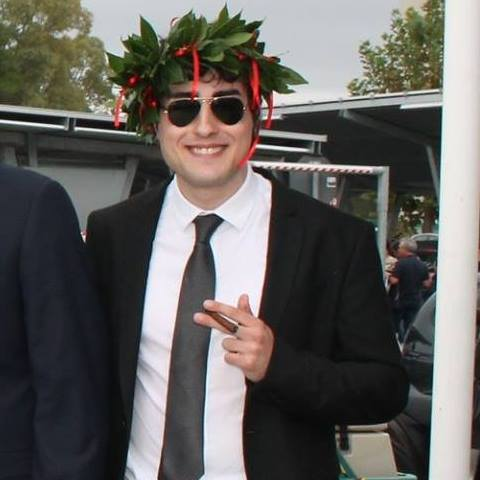
\includegraphics[width=3cm]{figures/marco.jpg}
\vspace{0.3cm}

\raisebox{-0.35ex}{
\includegraphics[width=4ex]{figures/link.png}}%
\hspace{0.05cm} /marcochiarelli

\end{figure}

\begin{figure}[h]

\includegraphics[width=3cm]{figures/gabriele.jpg}
\vspace{0.3cm}

\raisebox{-0.35ex}{
\includegraphics[width=4ex]{figures/link.png}}%
\hspace{0.05cm} /gabrieleaccarino

\end{figure}

\begin{figure}[h]

\includegraphics[width=3cm]{figures/paolo.jpg}
\vspace{0.3cm}

\raisebox{-0.35ex}{
\includegraphics[width=4ex]{figures/link.png}}%
\hspace{0.05cm} /paolo-panarese-6a016187

\end{figure}

\begin{figure}[h]

\includegraphics[width=3cm]{figures/emanuele.jpg}
\vspace{0.3cm}

\raisebox{-0.35ex}{
\includegraphics[width=4ex]{figures/link.png}}%
\hspace{0.05cm} /emanuele-costa-cesari-40ab1211a

\end{figure}


%BIBLIOGRAFIA - redatta con il relativo ambiente
\begin{thebibliography}{100}
\bibitem{rif1} G. Indiveri \emph{Notes on Rotations, Orientation Errors and Robot Kinematics}
\bibitem{rif2} G. Indiveri \emph{Introduzione alla tecnica dei Minimi Quadrati per l'identificazione parametrica e la stima dello stato}
\bibitem{rif3} G. Indiveri \emph{Ph.D Thesis, Chapter 3}
\bibitem{rif4} L. Sciavicco, B. Siciliano \emph{Robotica industriale}
\bibitem{rif5} A. Della Ducata \emph{Notazione di Denavit - Hartenberg}
\bibitem{rif6} L. Fortuna, M. Frasca \emph{Complementi di Teoria dei Sistemi e di Controlli Automatici}
\bibitem{rif7} T. I. Fossen, J. W. \& Sons \emph{Guidance and Control of Ocean Vehicles}
\bibitem{rif8} \emph{Handbook of (Marine) Robotics}
\bibitem{rif9} N. Newman \emph{Marine Hydrodynamics}
\end{thebibliography}

\end{document}


%************************************************
% Chapter 2: ROTAZIONI
%************************************************
% !TEX encoding = UTF-8
% !TEX TS-program = pdflatex
% !TEX root = ../rob.tex
% !TEX spellcheck = it-IT

%************************************************
\chapter{Rotazioni}
\label{cap:rot}
%************************************************\\

\section{Matrici di ROTAZIONE}

L'oggetto matematico che permette di descrivere la posizione di una terna rispetto ad un'altra è la matrice di ROTAZIONE.

\begin{defn}{\textbf{Matrice di ROTAZIONE}}

Dati due sistemi di riferimento $\{<0>,\ <1>\}$ indicati rispettivamente dalla seguente coppia di terne di versori mutuamente perpendicolari: $\{(i_0,j_0,k_0),\ (i_1,j_1,k_1)\}$, definiamo \textit{matrice di rotazione} tra il sistema $<0>$ ed il sistema $<1>$ (l'ordine di enunciazione delle terne è importante) il seguente oggetto matematico:

\[
	^1R_0 =
	\begin{bmatrix}^1i_0\in\R^{3\times 1}&^1j_0\in\R^{3\times 1}&^1k_0\in\R^{3\times 1}\end{bmatrix}
\]

dove, come graficamente esposto, i singoli elementi trascritti nella matrice sono dei vettori colonna. Ognuno di essi rappresenta il versore $i$-esimo, $i=1,2,3$ della terna $<0>$ espresso in terna $<1>$.

\end{defn}

Notiamo che:

\[
	\left\{
	\begin{aligned}
	&^0i_0 =  \begin{bmatrix}1&0&0\end{bmatrix}^\top\\
	&^0j_0 =  \begin{bmatrix}0&1&0\end{bmatrix}^\top\\
	&^0k_0 =  \begin{bmatrix}0&0&1\end{bmatrix}^\top
	\end{aligned}
	\right.
\]

$i_0$ è un versore. Oggetto di grandezza unitaria (in norma), il quale esiste a prescindere dalle sue componenti! I tre numeri conservano la MEMORIA in cui li ho calcolati. La matrice descrive l'assetto. Utile perché se conosco un vettore in una terna e voglio calcolare le sue componenti in terna $<1>$, è sufficiente effettuare questa operazione:

\[
	^1p =\ ^1R_0\ ^0p
\]

\`E semplicemente un prodotto matrice vettore. Ricordiamo che tale operazione è sostanzialmente una combinazione lineare degli elementi di una matrice (colonne) pesati con coefficienti forniti dal vettore con il quale si intende essa moltiplicare:

\[
	y = Mx = x_1m_1 + x_2m_2 +\ \dots\ + x_nm_n
\]

Una tale matrice di rotazione esprime l'assetto. Come è orientata la terna $<0>$ in terna $<1>$? Se prendiamo una direzione nota in terna $<0>$, e vogliamo vedere a cosa quella direzione corrisponde in terna $<1>$, è sufficiente utilizzare: $[^1p =\ ^1R_0\ ^0p]$, che corrisponderebbe alla proiezione in terna $<1>$ del vettore $^0p$. Quindi:

\[
	^1R_0 =
	\begin{bmatrix}{^1}i_0\in\R^{3\times 1}&^1j_0\in\R^{3\times 1}&^1k_0\in\R^{3\times 1}\end{bmatrix}
\]

Ovviamente, per via della disuguaglianza triangolare, ogni colonna deve sommare ad 1 in norma. Per essere una matrice di rotazione, i suoi elementi non saranno MAI maggiori di 1 in modulo! Tabellina di 9 numeri. Se li mettessimo random, molto probabilmente non otterremmo una matrice di rotazione! Ciascuna colonna ha esattamente NORMA 1! (Sono VERSORI!). Abbiamo tre $(1+1+1)$ vincoli relativi alla norma dei versori più tre altri vincoli $(1+1+1)$ relativi al fatto che, rispettivamente: $\{i\perp j,\ j\perp k,\ i\perp k\}$. Tabella di 9 numeri vincolata da 6 equazioni. Ne rimangono 3 altri gradi di libertà, pari quindi al numero di parametri minimi necessari a descrivere univocamente una matrice di rotazione. Rappresentazione minima: servono 3 numeri indipendenti (minimo) per (de)scrivere una matrice di rotazione. Come scegliere questi tre numeri è una storia abbastanza lunga. Alcuni ne scelgono 4 numeri al posto di 3 (QUATERNIONI). Altra caratteristica (tipicamente interconnessa alle altre): $^1p$ è una copia di $^0p$ MA in un altro sistema di riferimento. Ovviamente le componenti / orientazioni cambiano, ma la NORMA no! Dal punto di vista delle componenti, la NORMA di un vettore NON ha bisogno di loro! \`E semplicemente una funzione definita in maniera assiomatica, quindi una distribuzione in tal senso:

\[
	\norma{x}:\R^n\mapsto \R\ |\\
	\left\{
	\begin{aligned}
	&\norma{x} \geq 0,\ \norma{x} = 0 \iff x=0\\
	&\norma{x+y} \le \norma{x}+\norma{y}
	\end{aligned}
	\right.
\]

\`E in realtà a nostra discrezione come definirla! Se questa "turca" funzione soddisfa alle seguenti condizioni, allora è una norma! La norma euclidea è una qualsiasi norma possibile tra le tante (infinite). \`E calcolabile comodamente mediante l'utilizzo delle componenti:

\begin{corl}{\textbf{Calcolo della norma di un vettore mediante componenti}}

\[
	[\norma{x}^2 = X_x^2 + X_y^2 + X_z^2]
\]

\end{corl}

Ma anche le norme, ovviamente, prescindono anch'esse dalle componenti dei vettori. Infatti una definizione più pragmatica e rigorosa è la seguente, della quale il risultato precedente è infatti un corollario:

\begin{defn}{\textbf{Norma di un vettore}}

\[
	[\norma{p\in\R^{3\times 1}}_2 = \sqrt{p^\top p}]
\]

\end{defn}

Proviamo ad applicare la seguente definizione al vettore: $^1p$:

\[
	\norma{^1p}^2 =\ ^1p^\top\ ^1p =\ ^0p^\top\ ^1R_0^\top\ ^1R_0\ ^0p \stackrel{ISOMTRC}{=}\ ^0p^\top\ ^0p = \norma{^0p}^2
\]

Risultato che mostra che la matrice di rotazione esprime una trasformazione ISOMETRICA. Questo risultato naturalmente, wlog, vale $\forall\ ^1p$! Ciò significa che:

\begin{defn}{\textbf{Unitarietà di una matrice di rotazione}}

\[
	^1R_0^\top\ ^1R_0 = I_{3\times 3}
\]

\begin{itemize}
\item La matrice $^1R_0$ è INVERTIBILE! Ovvero ha sempre rango pieno;
\item La sua inversa concide con la TRASPOSTA. (Definizione di matrice unitaria, la quale in campo complesso indica che l'inversa coincide con la TRASPOSTA (COMPLESSA) CONIUGATA, mentre in campo reale indica proprio la definizione appena esplicitata, e si parla di matrice ORTONORMALE).
\end{itemize}

\end{defn}

Le MATRICI UNITARIE, come appena visto, sono \underline{isometriche}. Le operazioni isometriche (lineari, descritte da matrici), sono sicuramente legate a MATRICI UNITARIE. Se lo pensiamo in termini di definizione di $^1R_0$, allora il risultato è OVVIO!

\[
	^1R_0^\top\ ^1R_0 =
	\begin{bmatrix}^1i_0^\top\ ^1i_0 = 1 & 0 & 0\\0 & ^1j_0^\top\ ^1j_0 = 1 & 0\\0 & 0 & ^1k_0^\top\ ^1k_0 = 1\end{bmatrix} = I_{3\times 3}
\]

Adoperiamo ora l'applicazione del teorema di Binet sul determinante di un prodotto: per una matrice quadrata, abbiamo che il determinante della matrice prodotto è pari al prodotto dei determinanti delle singole matrici. Inoltre sappiamo che il determinante della matrice trasposta è pari al determinante della matrice in esame. Mettendo insieme ambo le cose, otteniamo:

\[
	(\det{R})^2 = 1 \implies \det{R} = \pm 1
\]

Il determinante di $R$ è quindi: $\{+1,\ -1\}$. Tutte le matrici unitarie hanno determinante di valore assoluto pari ad 1. Riassumiamo quindi i seguenti fatti:

\begin{itemize} 

\item Tutte le matrici unitarie hanno sicuramente $(\det{R})^2 = 1$;
\item Le ROTAZIONI hanno determinante della matrice di rotazione pari a $(+1)$;
\item Le RIFLESSIONI (quando ci guardiamo allo specchio es.) hanno determinante pari a $(-1)$.

\end{itemize}

Non esiste difatti una rotazione che possa eseguire il mapping relativo ad un'operazione di riflessione. Anche le RIFLESSIONI però conservano la norma, sono quindi pure loro delle isometrie. Supponiamo ora di avere: $h\in\R\ |\ \norma{h}=1$ un versore (vettore di norma unitaria). Consideriamo la seguente matrice di trasformazione:

\[
	Q = I_{3\times 3} - 2hh^\top
\]

Proviamo ad applicarla ad un vettore $v$:

\[
	Qv = (I_{3\times 3} - 2hh^\top)v = v - 2hh^\top v
\]

\begin{itemize}

\item Se $v=h \implies Q(v=h) = -h$ (il vettore $h$ semplicemente cambia segno);
\item Se $(v\perp h \iff v^\top h=h^\top v=0) \implies Qv = v$;

\end{itemize}

Supponiamo di avere un vettore $h = \begin{bmatrix}1&2&7\end{bmatrix}^\top$. Abbiamo che:

\[
	hh^\top = \begin{bmatrix}1&2&7\end{bmatrix}^\top \begin{bmatrix}1&2&7\end{bmatrix} = \begin{bmatrix}1&2&7\\2&4&14\\7&14&49\end{bmatrix}
\]

Notiamo che tale matrice è simmetrica, ma ovviamente si poteva già vedere dal fatto che: $(2hh^\top)^\top = 2hh^\top$. Calcoliamo ora:

\[
	Q^\top Q = (I-2hh^\top)^\top (I-2hh^\top) = I - 2hh^\top - 2hh^\top + 4h(h^\top h = 1)h^\top = I_{3\times 3}
\]

$Q$ è una matrice simmetrica $\impliedby Q^\top = Q$. $Q$ è un'ISOMETRIA. Questa matrice $(Q\in\R^{3\times 3})$ conserva la norma, la lunghezza. $h$ è arbitrario. Basta che sia un versore, a norma 1. NON tutte le ISOMETRIE sono delle rotazioni! Prende un vettore e cambia soltanto il segno delle componenti lungo l'asse ortogonale al piano! Questa è proprio una riflessione!

La trasformata risultante è: trasforma una terna destrorsa in una sinistrorsa. $\nexists$ modo di ruotare una terna per far diventare una terna destrorsa in una sinistrorsa. $(\det{Q}=-1)$. Non tutte le matrici ISOMETRICHE sono delle rotazioni. Esistono operazioni isometriche che non sono delle rotazioni, come appena visto.

$A^\top A = I \implies A$ ISOMETRIA. Tutte le matrici ISOMETRICHE in $\R^n$ hanno determinante della matrice associata $+1$ o $-1$. Le ROTAZIONI sono delle isometrie particolari a determinante $(+1)$.

\begin{defn}{\textbf{Gruppo delle MATRICI ORTONORMALI}}

\[
	\underline{\Theta(n)} = \{M\in\R^{n\times n}\ |\ MM^\top = M^\top M = I_{n\times n}\}
\]

\end{defn}

Prendiamo un paniere delle tali matrici appena definite. Il termine sottolineato è l'insieme delle matrici ortonormali in $\R^n$. Tale oggetto è un gruppo. Gode delle proprietà di gruppo:

\begin{itemize}

\item $\exists$ elemento unitario;
\item Il gruppo è chiuso rispetto al prodotto;
\item associatività (possiamo "spostare" le parentesi).

\end{itemize}

Con i gruppi si può astrarre, ed ottenere delle proprietà particolari per degli oggetti che siano gruppi. $\Theta(n)$ è il gruppo delle trasformazioni isometriche. Un generico elemento che vi appartiene ha determinante $\{+1,\ -1\}$. Lì dentro ci sono pure le rotazioni.

\begin{defn}{\textbf{Gruppo delle rotazioni $\SO(n)$}}

\[
	\SO(n) = \{M\in\R^{n\times n}\ |\ M^\top M = MM^\top = I_{n\times n},\ \underline{\det{M}} = +1\}
\]

\end{defn}

Sicuramente tali matrici sono delle matrici di ROTAZIONE. Matrici speciali ortonormali di ROTAZIONE in $\R^n$. \underline{MATRICI ISOMETRICHE} a determinante $(+1)$; (conservano le lunghezze). $\SO(n)$ è ANCORA UN GRUPPO! Fondamentale. Due matrici di rotazione diverse, se moltiplicate, restituiscono in output una matrice ancora appartenente al gruppo. Eredita quindi l'elemento identico di $\Theta(n)\ (I_{n\times n}\in\R^{n\times n})$. Esiste l'INVERSA, e coincide con la TRASPOSTA, dato che le matrici in gioco sono unitarie. 

Ricordiamo ora le proprietà delle trasformazione di riflessione:

\[	
	\left\{
	\begin{aligned}
	&Qh = -h\\
	&Qv = v \impliedby (v\perp h)
	\end{aligned}
	\right.
\]

Ricordiamo che: $^1p =\ ^1R_0\ ^0p$. Definiamo ora l'operazione di PROIEZIONE:

\begin{defn}{\textbf{\underline{OPERATORE PROIETTORE}}}

with: $h\in\R^{n\times n},\ \norma{h}=1$:

\[	
	M = I_{n\times n} - hh^\top
\]

\end{defn}

Con la seguente matrice prendiamo un versore in $\R^n$ (vettore di norma 1) e ne tagliamo tutte le componenti lungo $h$. Abbiamo:

\begin{itemize}

\item $Mh = 0$;
\item $M(v\perp h) = v$;

\end{itemize}

In un problema di CINEMATICA è scomodo portarsi dietro una matrice di 9 numeri. Solo 3 numeri SONO indipendenti! \`E più comodo manipolare non tutti gli elementi della matrice, ma solo i parametri MINIMI! La Scelta è però NON univoca. $\exists\infty$ modi per individuare tre parametri per descrivere una data matrice di rotazione. Bisogna introdurre una rappresentazione, la RAPPRESENTAZIONE ESPONENZIALE delle matrici di ROTAZIONE. Solo in $\R^3$ (In $SO(3)$ i suoi elementi possono essere rappresentati in tal modo).

\subsection{Matrici simmetriche / antisimmetriche} 

\begin{thrm}{\textbf{Decomposizione simmetrica/antisimmetrica di una matrice}}

\[
	[(M\in\R^{3\times 3}) = \frac{M+M^\top}{2} + \frac{M-M^\top}{2}]
\]

\end{thrm} 

\`E un risultato interessante perché il primo termine è SIMMETRICO (matrice uguale alla sua trasposta $\iff A=A^\top$), mentre è ANTISIMMETRICO il secondo (matrice uguale a MENO la sua trasposta $\iff A=-A^\top$).

Le matrici ANTISIMMETRICHE hanno una proprietà molto particolare. Mappano i vettori in tal modo:

\[
	x^\top (Ax) \stackrel{REAL}{=} (x^\top Ax)^\top \stackrel{TRANSP}{=} x^\top A^\top x \stackrel{SKEWSYMM}{=} -x^\top(Ax) = 0
\]

ove come annotato sopra l'uguale, esso vale dal momento che $(x^\top Ax)\in\R\ \forall A\in\R^{n\times n}$. Le matrici ANTISIMMETRICHE mappano il vettore ($A$ potrebbe pure non essere isometrica ovviamente) ortogonalmente ad esso. Le matrici ANTISIMMETRICHE in $\R^{n\times n}$ godono di questa particolare proprietà.

\subsection{Skew-symmetry}

Teniamo a mente la seguente:

\[	
	M\in\R^{n\times n}\ |\ M = \frac{M+M^\top}{2} + \frac{M-M^\top}{2}
\]

Posti $a,b\in\R,\ c=a\times b \leftarrow$ (operazione lineare). 

\[
	c\mapsto \begin{vmatrix}i&j&k\\a_1&a_2&a_3\\b_1&b_2&b_3\end{vmatrix} = \underline{i}(a_2b_3 - a_3b_2) - \underline{j}(a_1b_3 - a_3b_1) + \underline{k}(a_1b_2 - a_2b_1)
\]

Gli elementi di quella matrice sono associati a componenti del vettore. Abbiamo:

\[
	S(\underline{a}\in\R^{3\times 1})\in\R^{3\times 3}
\]

Matrice $\R^{3\times 3} \ni S(\underline{a})$ che rappresenta l'operazione di prodotto vettore (se opportunamente moltiplicato per un altro vettore, opportuno). Matrice ANTISIMMETRICA. $\underline{a}$ si chiama anche VETTORE ASSIALE della matrice ANTISIMMETRICA. Qualsiasi matrice antisimmetrica ha associato un UNICO vettore assiale. Il modo banale di vederlo è che, prendendo una qualsiasi matrice random, estraendone la parte antisimmetrica $(\frac{M-M^\top}{2})$, ha sempre 0 sulla diagonale principale. Scegliendo a caso $\{a_1,\ a_2,\ a_3\}$, allora abbiamo quindi la corrispondenza: VETTORE ASSIALE $\leftrightarrow$ MATRICE ANTISIMMETRICA. Quei 3 numeri li interpretiamo come componenti del vettore assiale associato. Dimostrazione sulle dispense più efficiente (non passa per le componenti). In realtà un OPERATORE LINEARE prescinde anch'esso dalle componenti! Ha delle particolari proprietà. La dimostrazione si può fare senza fare uso delle componenti! Il prodotto vettore in $\R^3$ definisce un unico vettore assiale di una matrice antisimmetrica (e viceversa). Il risultato di $Ax$ è esprimibile mediante prodotto vettore, e viceversa:

\begin{thrm}{\textbf{Skew-symmetry Matrix and Axial Vector Mapping}}

\[
	\left\{
	\begin{aligned}
	&Ax = a\times x\\
	&a,x\in\R^{3\times 1}\\
	&(A=-A^\top)\in\R^{3\times 3}
	\end{aligned}
	\right.
\]

\end{thrm}

Dimostrazione costruttiva, senza componenti. Obiettivo: Dimostrare che $A$ è ANTISIMMETRICA: $\exists! \underline{a}\ |\ Ax=\underline{a}\times \underline{x}$. Utilizzando le componenti è abbastanza banale, già dimostrato.

\begin{proof}

\[
	\underline{a} = \frac{1}{2}\sum_{i=1}^3{e_i\times Ae_i} = (\dots)
\]

Bisogna applicare le proprietà del prodotto vettore, e ad un certo punto ovviamente la proprietà di antisimmetria per $A$. Chiamiamo con $e_i$ il generico versore $i$-esimo dello spazio $\R^3$ (individuiamo una base ortonormale arbitraria di $\R^3$). Segue:

\[
	\underline{a}\times\underline{x} = \underline{\frac{1}{2}[\sum_{i=1}^3{(e_i\times Ae_i)]}}\times\underline{x} = \frac{1}{2}\sum_{i=1}^3{(\underline{x}\times(Ae_i\times e_i))} = (\dots)
\]

Ove abbiamo cambiato l'ordine del prodotto vettore due volte onde evitare il segno. Si rammenti la regola del TRIPLO PRODOTTO:

\[
	a\times(b\times c) = b(a^\top c) - c(a^\top b)
\]

Sempre vera. L'ordine nel prodotto vettore conta! Si effettui prima $(b\times c)$, e lo si moltiplichi secondo prodotto vettore per $\underline{a}$. Quindi, tornando a noi:

\[
	(\dots) = \frac{1}{2}\sum_i{[\underline{(Ae_i)(x^\top e_i)} - e_i(x^\top Ae_i)]} = (\dots)
\]

Ove il termine sottolineato sommato ad $i$ restituisce proprio $Ax$, per definizione. Ora applichiamo l'antisimmetria.. se anziché $x^\top Ae_i$ ne mettessimo la versione invertita, allora esso cambierebbe segno. Fino ad ora abbiamo fatto semplicemente del calcolo generico.

\[
	(\dots) \stackrel{SKEWSYMM}{=} [\frac{1}{2}(Ax + \underline{\sum_i{e_i((Ax)^\top e_i)}}] = \frac{Ax}{2}+\frac{Ax}{2} = Ax
\]

\end{proof}

Ove il termine sottolineato è sempre $Ax$. Ciò chiude la dimostrazione. Questo vettore assiale $\underline{a}$ è UNICO! Dimostrazione semplice per esercizio. Non è molto standard, ma l'operazione che mappa una matrice antisimmetrica nel suo vettore assiale è la seguente, definita mediante il seguente mapping:

\[
	\Vex(A) = \underline{a}\in\R^{3\times 1}
\]

Abbastanza pesante come notazione, ma non infrequente in letteratura. Pseudo-vettore in realtà. Nell'ambito delle rotazioni il vettore assiale lo incontreremo abbastanza di frequente. $\underline{a}=\begin{bmatrix}a_1&a_2&a_3\end{bmatrix}^\top$. La matrice $A$, è quindi:

\[
	A := S(\Vex(A)) = S(\underline{a}) =
	\begin{bmatrix}0&-a_3&a_2\\a_3&0&-a_1\\-a_2&a_1&0\end{bmatrix}
\]

Se una tale matrice $A$ fosse ad esempio: $A:=\begin{bmatrix}0&3&2\\-3&0&-1\\-2&+1&0\end{bmatrix}$, allora il suo vettore assiale sarebbe: $Vex(A):=\underline{a}=\begin{bmatrix}1&2&-3\end{bmatrix}^\top$. Sul segno vi è in realtà un po' di ambiguità, ma non relativamente al vettore assiale in sé per sé.

La regola del triplo prodotto è stata molto utile, e sarà tale ancora durante il prosieguo del corso:

\begin{thrm}{\textbf{Regola del TRIPLO PRODOTTO}}

\[
	\underline{a}\times(\underline{b}\times\underline{c}) = \underline{b}(a^\top c) - \underline{c}(a^\top b) = (\dots)
\]

\end{thrm}

Questo fatto mette in evidenza che questa operazione tra vettori, ne freeza due e tratta il terzo come parametro (costante); l'operazione è quindi lineare. Banale dimostrarlo:

\[
	[(\dots) = (I_{3\times 3}(a^\top c) -\underline{c}\underline{a}^\top \in\R^{3\times 3})\underline{b}]\in\R^{3\times 1} = (\dots)\\
\]

Rispetto $\underline{b}$ lo posso scrivere come matice per $\underline{b}$. Se fossero $\underline{a}$, o $\underline{c}$ liberi, avremmo:

\[
	\left\{
	\begin{aligned}
	&(\dots);\\
	&(\dots) = (\underline{b}\underline{c}^\top -\underline{c}\underline{b}^\top)\underline{a};\\
	&(\dots) = [\underline{b}\underline{a}^\top -I_{3\times 3}(\underline{a}^\top\underline{b})]\underline{c};
	\end{aligned}
	\right.
\]

Operatore lineare su uno dei tre argomenti. Su qualche passaggio cinematico tornerà utile. Regola del triplo prodotto banalmente dimostrabile per calcolo diretto. Mostriamo un po' di \emph{sugar calculus}:

\[
	\left\{
	\begin{aligned}
	&\{\Vex(A),\ \underline{S^\top(\underline{a}) = -S(\underline{a})}\}\\
	&[\Vex(A)=\underline{a} \implies \Vex[S(\underline{a})] = \underline{a}]
	\end{aligned}
	\right.
\]

\subsubsection{Proprietà di una Matrice Antisimmetrica}

\`E utile sapere che la potenze di una matrice antisimmetrica hanno una particolare ricorsione. Calcolabile di nuovo per calcolo diretto:

\[	
	\{S(\underline{a})S(\underline{a}) := S^2(\underline{a}),\ S(\underline{a})S(\underline{a})S(\underline{a}) := S(\underline{a})^3,\ \dots\}
\]

Ad occhio vengono fornite le seguenti formule. Dato: $\underline{h}\in\R^{3\times 1}\ |\ \norma{h}=1$ VERSORE, abbiamo:

\[
	\left\{
	\begin{aligned}
	&S(\underline{h}) = \underline{h}\times\mathord{\cdot}\\
	&S^2(\underline{h}) = hh^\top - I_{3\times 3}\\
	&S^3(\underline{h}) = -S(\underline{h})\\
	&S^4(\underline{h}) = -S^2(\underline{h})
	\end{aligned}
	\right.
\]

Possiamo generalizzare:

\begin{thrm}{\textbf{Potenze di una MATRICE ANTISIMMETRICA}}

\[
	\left\{
	\begin{aligned}
	&S^{2i+1}(\underline{h}) = (-1)^iS(\underline{h})\\
	&S^{2(i+1)}(\underline{h}) = (-1)^i(\underline{hh^\top -I_{3\times 3}})
	\end{aligned}
	\right.
\]

\end{thrm}

Ricordiamo che $(I_{3\times 3} - hh^\top)$ è il proiettore. Quindi il termine sottolineato è il proiettore cambiato di segno. Per alcune potenze pari (precisamente le potenze pari di esponente $i$ dispari), sarà proprio il proiettore, per le altre sarà il proiettore cambiato di segno, per l'appunto.

$S(\underline{h})v=h\times v,\ \Tr(S(\underline{h})=0)$. La traccia delle potenze dispari continuerà quindi ad essere 0. La traccia delle potenze pari, data la traccia particolare che $hh^\top$ esibisce ovvero $\Tr(hh^\top) = h^\top h=1$, ha la seguente espressione:

\[
	[\Tr(S^{2(i+1)}(\underline{h})) = (-1)^{i+1}2]
\]

Ulteriore proprietà: stupidaggine ma fino ad un certo punto: verrà comoda più in avanti. \`E la seguente: $\forall$ matrice antisimmetrica $\mathord{\cdot}\in\{\R^{3\times 3}\}$ è associato un UNICO VETTORE ASSIALE!

Ora prendiamo $\{\exists M\in\R^{3\times 3},\ \underline{x}\in\R^{3\times 1}\}$.
Eventualmente $M$ può anche essere a simmetria non ben definita. Calcoliamo la trasposta della matrice ottenuta a valle dell'applicazione della trasformazione di similitudine:

\[
	(M\underline{S(\underline{x})}M^\top)^\top = MS(\underline{x})^\top M^\top = -MS(\underline{x})M^\top
\]

$\implies [MS(\underline{x})M^\top]$ antisimmetrica! Essendo antisimmetrica, deve ammettere un vettore assiale: 

\begin{thrm}{\textbf{Trasformazione di similitudine di una Matrice Antisimmetrica}}

\[
	\left\{
	\begin{aligned}
	&MS(\underline{x})M^\top = S(\underline{y})\\
	&y = (L\in\R^{3\times 3})x
	\end{aligned}
	\right.
\]

\end{thrm}

$(L\in\R^{3\times 3})$ è stata già calcolata. Usiamo la notazione \emph{MATLAB}, ove $M(2,:)$ indica la seconda riga (quindi in versione trasposta rappresenterebbe un vettore colonna); ad esempio il termine citato prima corrisponde alla riga selezionata della matrice $M$ così parametrizzata:

\[
	\begin{bmatrix}m_{11}&m_{12}&m_{13}\\\underline{m_{21}}&\underline{m_{22}}&\underline{m_{23}}\\m_{31}&m_{32}&m_{33}\end{bmatrix}
\]

abbiamo:

\[
	L = \begin{bmatrix}\begin{bmatrix}M(2,:)^\top\times M(3,:)^\top\end{bmatrix}^\top\\\begin{bmatrix}M(3,:)^\top\times M(1,:)^\top\end{bmatrix}^\top\\\begin{bmatrix}M(1,:)^\top\times M(2,:)^\top\end{bmatrix}^\top\end{bmatrix}
\]

$M$ è la più generale possibile. Se prendiamo per $M$ un elemento di $\SO(3)$ (matrice di rotazione), la $L$ associata è proprio $M$! Ovvero la tale matrice di rotazione scelta. A valle dell'analisi, del tutto generale, ricaviamo un utilissimo risultato particolare. Prendiamo una generica matrice di rotazione:

\begin{corl}{\textbf{Trasformazione di similitudine di una Matrice Antisimmetrica}}

$R\in\SO(3),\ \forall x\in\R^{3\times 1}$:

\[
	[RS(\underline{x})R^\top = S(Rx)]
\]

\end{corl}

\`E un risultato abbastanza semplice. Dal punto di vista algebrico è come abbiamo detto prima. In $\SO(3),\ L=R$. Un interpretazione geometrica è molto profonda. Una rotazione, dal punto di vista geometrico, è un'ISOMETRIA (che CONSERVA le distanze), che conserva il PRODOTTO VETTORE. Le rotazioni fanno sì che le distanze relative tra due punti fissi rimangano uguali! Trasformazione di similitudine:

\[
	\underline{RS(\underline{x})R^\top = S(R\underline{x})}
\]

$\leftarrow$ le rotazioni conservano il prodotto vettore: ruotando il risultato del prodotto vettore è la stessa cosa del ruotare singolarmente, isolatamente l'operando sinistro di esso (del prodotto vettore). \`E un risultato in realtà abbastanza potente!

Possiamo adesso analizzare un legame profondo e significativo tra gli elementi di $\SO(3)$ e le \underline{matrici esponenziali}:

\subsection{Matrici ESPONENZIALI}

\begin{defn}{\textbf{Matrice ESPONENZIALE}}

$M\in\R^{n\times n}\ \theta\in\R,\ \forall i,j$

\[
	(L = \e^{M\theta}\in\R^{n\times n}) := (\underline{\sum_{l=0}^{+\infty}{\frac{M^l\theta^l}{l!}}}) < +\infty \iff e^{M\theta}_{ij} <+\infty
\]

\end{defn}

Tale matrice è nientemeno che la matrice $e^{At}$ vista in TdS. $\e$ è proprio il simbolo di Nepero in tal caso, ma stavolta rappresenta una matrice intesa come autofunzione rispetto ad operatori differenziali, come vedremo dalle prossime proprietà.
La sommatoria tra parentesi tonde CONVERGE sicuramente! La sommatoria rappresenta infinite potenze, scalate per $\frac{1}{l!}$ e sommate. Converge ad una quantità finita, ovvero in tal caso ad una matrice con elementi tutti finiti. Come già anticipato, il motivo per cui utilizziamo questa notazione è che, non solo ricorda Taylor, ma questa matrice qui gode di parecchie proprietà, molte delle quali analoghe a quelle dell'esponenziale scalare.

\subsubsection{Proprietà della Matrice Esponenziale}

Dal punto di vista concettuale le seguenti proprietà sono molto profonde:

\begin{itemize}

\item La matrice $\e^{M\theta}$ è sempre INVERTIBILE, $\forall M$ anche NON INVERTIBILE!
\item Al posto di $M$, mettendovi $-M$, ed eseguendo l'esponenziale matriciale otteniamo l'inversa di $(\e^{M\theta})$:
$\inv{(\e^{M\theta})} = \e^{-M\theta}$;
\item $(\e^{M\theta})^\top = \e^{M^\top\theta}$;
\item $[\underline{M\e^{M\theta} = \e^{M\theta}M}]$.

\end{itemize}

Le matrici generiche tra di loro non commutano generalmente rispetto al prodotto matriciale. L'ultima proprietà è un risultato abbastanza stupido: si ottiene semplicemente moltiplicando per $M$ ambo i membri della definizione, e vedendo cosa si ottiene nell'RHS..

La matrice non è tuttavia banale da calcolare generalmente. Una delle sue possibili difficoltà è che le potenze non hanno una struttura semplice o ben definita. Ci sono alcuni casi invece semplici e banali, ad esempio nel caso di matrici $M$ NILPOTENTI (dopo alcune potenze diventano 0) oppure IDEMPOTENTI. Se è diagonalizzabile ci sono invece altri trucchi, legati alla costruzione delle cosiddette matrici di JORDAN, LAPLACE, etc.. Se $l=17$, abbiamo 17 termini nella sommatoria matriciale.

Notazioni matematiche: $\{\{h\in\R^{3\times 1},\ \norma{h}=1\},\ SCALAR\ \theta\in\R\}$. Calcolando:

\[
	[\underline{\e^{\theta S(\underline{h})} \in\R^{3\times 3}}] \in\SO(3)
\]

Vi è un legame SURGETTIVO sostanzialmente. Vale un risultato fondamentale, dimostrato da Eulero nel 1700. Possiamo ricoprire tutto $\SO(3)$. $\forall$ elemento di $\SO(3)$, ammette tanti $\theta,\ \underline{h}$ tale per cui valga l'appartenenza al gruppo prima esplicitata. La ricopertura è addirittura troppo buona! Nel senso che, vi sono diversi modi (parametri) per giungere allo stesso elemento di $\SO(3)$, come vedremo più in avanti.

\subsubsection{Rappresentazione esponenziale delle Matrici di Rotazione}

Tale sottosezione è di una notevole importanza pratica! Praticamente ENORME! Non solo dal punto di vista teorico. Tale formula tuttavia non ci dice ancora niente. Proprio perché la matrice esponenziale è difficile da calcolare $(\e^{\theta S(\underline{h})})$. In realtà quella formula si può semplificare (RODRIGUES). Dobbiamo dimostrare anzitutto che:

\begin{thrm}{\textbf{Appartenenza ad $\SO(3)$ delle Matrici Esponenziali (Speciali)}}

\[
	[\e^{\theta S(\underline{h})}\in\SO(3)]
\]

\end{thrm}

\begin{proof}


\begin{itemize}

\item{\textit{Unitarietà della matrice}}:

\[
	(\e^{\theta S(\underline{h})})^\top(\e^{\theta S(\underline{h})}) \stackrel{EXP}{=} \e^{\theta S^\top(\underline{h})}\e^{\theta S(\underline{h})} = (\dots)
\]
\[
	(\dots) = \e^{\theta (S^\top(\underline{h}) + S(\underline{h}))} = \stackrel{SKEWSYMM}{=} \e^{\theta(-S(\underline{h})+S(\underline{h}))} \stackrel{EXPINV}{=} I_{3\times 3}
\]

\item{\textit{Determinante positivo unitario}}:

Abbiamo anche dimostraro che, per Binet, il determinante al quadrato è 1! $(\det(\e^{\theta S(\underline{h})}) = \pm 1)\ \forall\theta\forall h$! Come facciamo a dimostrare che è proprio $+1$ e non $-1$? Il determinante di una matrice è una funzione continua dei suoi elementi. Se sapessimo scrivere $(\e^{\theta S(\underline{h})})$ (i suoi singoli elementi), ci aspetteremmo che essa sia una funzione di 4 numeri, di 4 parametri: $(\begin{bmatrix}h_1&h_2&h_3\end{bmatrix}^\top, \theta)$. Il determinante sarà o costantemente $+1$, o costantemente $-1$. \`E una funzione continua dei suoi parametri. Se prendiamo $(\theta=0)$, abbiamo:

\[
	(\e^{0S(\underline{h})} = I_{3\times 3})
\]

il cui determinante è proprio $(+1)$! In un punto quindi il determinante lo sappiamo calcolare, e lo abbiamo calcolato in maniera esatta. $+1$ ovunque. Relativamente sottile come ragionamento, ma non difficile. Tale risultato, ricapitolando, si ottiene mettendo insieme due cose:

\begin{itemize}

\item Determinante in modulo unitario;
\item Determinante funzione continua degli elementi della matrice.

\end{itemize}

\end{itemize}

\end{proof}

In questa definizione non abbiamo supposto che $h$ fosse un VERSORE. VETTORE GENERICO. Per comodità (wlog), si utilizzerà $h\ |\ \norma{h}=1$.

\subsubsection{Formula di Rodrigues}

Se prendiamo la formula dell'esponenziale matriciale, riscrivendola:

\[
	[\e^{\theta S(\underline{h})} \in\SO(3)]
\]

Mi ricordo della definizione di matrice esponenziale. La riscrivo computandola per esteso, trovando:

\begin{defn}{\textbf{FORMULA DI RODRIGUES}}

\[
	\e^{\theta S(\underline{h})} = I_{3\times 3} + \sum_{l=1}^{+\infty}{\frac{S^l(\underline{h})}{l!}\theta^l} \stackrel{REC.SKEWPOWER}{=} (\dots)
\]
\[
	(\dots) = [I_{3\times 3} + \sin(\theta) S(\underline{h}) + (1-\cos(\theta))S^2(\underline{h})]
\]

\end{defn}

ove si è utilizzato nell'ultimo passaggio della definizione le formule delle potenze di $S(\underline{h})$, trovando il risultato esposto per semplice pura ispezione visiva.

A questo punto la matrice di rotazione la riusciremo a scrivere! Con carta e penna, MATLAB, C, Java, etc. Ad esempio: $\{h\ VERSORE\ |\ \norma{h}=1\},\ \theta=35^{\circ}$. Disponendo quindi dei seguenti elementi: $\{h,\theta\} \leftrightarrow$ \{versore dell'asse, angolo di rotazione\}, riusciamo quindi a scrivere la matrice di rotazione. La formula di Rodrigues è stata quindi ottenuta dal riconoscimento dello sviluppo in serie di Taylor delle funzioni trigonometriche applicato alla scrittura delle varie potenze della matrice antisimmetrica. Va detto che $h$ è il versore dell'asse di rotazione. Dev'essere un autovettore di $R$ con autovalore associato $1$, dal momento che abbiamo la seguente direzione preferenziale:

\[
	(\e^{\theta S(\underline{h})}\underline{h}) = \underline{h}
\]

$h$ è quindi la direzione dell'asse di rotazione. $\theta$ dev'essere necessariamente l'angolo. Ci rimane da chiederci: se prendo un generico elemento di $\SO(3)$, $\exists h\in\R^{3\times 1}\ |\ \norma{h}=1,\ \theta\in\R$ tale per cui esista una matrice esponenziale $\e^{\theta S(\underline{h})}$ che lo rappresenti? Ruotare di $(\theta=0^{\circ})$ vuol dire avere infiniti $h$ (qualsiasi asse possibile). Per scrivere problemi di controllo, ad esempio l'orientazione di un satellite, mi calcolo dei parametri delle posizioni finali. Mi calcolo la \underline{fdt $h(t)$} (se fosse lineare), la quale avrebbe matematicamente una SINGOLARIT\`A. \`E un problema di Rappresentazione, NON problema fisico. Le Rappresentazioni esponenziali delle matrici di rotazione hanno questi problemi (NON-UNIVOCIT\`A, ovvero SINGOLARIT\`A in gioco).

\subsubsection{Mapping SURGETTIVO}

Abbiamo un mapping surgettivo tra la matrice exp e gli elementi in $\SO(3)$. Ricordiamo che:

\[
	\e^{S(\underline{h})\theta} = I_{3\times 3} + \sin(\theta)S(\underline{h}) + (1-\cos(\theta))S^2(\underline{h})
\]

con $\underline{h}\in\R^{3\times 1},\ \norma{h}=1,\ \theta\in\R$. La sopracitata formula di Rodrigues vale $\forall\theta\forall \underline{h}$. Il problema è notare che esistono infiniti $\theta$ e $\underline{h}$ che consentono di individuare elementi in $\SO(3)$. Notiamo che scelto $(\theta\in\R)$, si potrebbe ottenere la stessa matrice exp andando a scalare $\theta$ di un fattore $2k\pi$, giacché le funzioni trigonometriche in gioco sono periodiche di periodo $2\pi$. NB: Il legame tra l'evoluzione temporale di un matrice di rotazione ed i suoi parametri $\{\underline{h},\ \theta\}$ che la descrivono non è banale! Occorre definire il fattore integrante: il vettore velocità angolare. Occorre focalizzarsi sulla posa iniziale e quella finale, ma non si hanno gli strumenti per descrivere la traiettoria.

Ogni matrice quadrata $n\times n$ è decomponibile nella somma di una parte simmetrica e di una antisimmetrica, e questo si evince anche nella formula di Rodrigues. Data una matrice arbitraria $R\in\SO(3)$, abbiamo:

\[
	[\Vex(\frac{R-R^\top}{2}) = \sin(\theta)\underline{h}]
\]

Se calcoliamo la traccia di $\e^{S(\underline{h})\theta}$, noteremo che la parte antisimmetrica non dovrebbe contribuire, dal momento che tale matrice ha tutti 0 sulla diagonale principale.

\[
	\left\{
	\begin{aligned}
	&S^2(\underline{h}) = hh^\top - I_{3\times 3}\\
	&\Tr(S^2(\underline{h})) = -2
	\end{aligned}
	\right.
\]

Eguagliamo ora la traccia di $R$ con quella di $\e^{\theta S(\underline{h})}$:

\[
	\Tr(R) = 3 + 0 -2(1-\cos(\theta)) = 1+2\cos(\theta) \implies
	\left\{
	\begin{aligned}
	&\centernot{2}cos(\theta) = \frac{tr(R)-1}{2}\\
	&\theta h = \frac{\theta}{\sin(\theta)} \Vex(\frac{R-R^\top}{2})
	\end{aligned}
	\right.
\]

Ma la prima equazione del sistema non è $\theta$! Dobbiamo quindi estrarre l'arcocoseno; ma quando lo estraiamo, il modulo è ben definito, ma non il segno! Il problema è che se $\theta=0$, sostituito nella seconda equazione fornisce:

\[
	\Vex(\frac{R-R^\top}{2}) = \sin(\theta)\underline{h} = 0 \implies [R=I]
\]

Non riesco quindi ad individuare un $\underline{h}$ univoco, infatti esso può essere qualsiasi con $\theta=0^{\circ}$! ($\exists\ MUL\ \underline{h}$). L'ambiguità sta in come trattiamo i parametri che sono 4: $\{h_x,\ h_y,\ h_z,\ \theta\}$. Infatti le componenti di $h$ sono dipendenti per la condizione di NORMALIZZAZIONE $\iff \norma{h}=1$; $\underline{h}$ ha due componenti linearmente indipendenti. $\underline{h}$ è un versore, le sue componenti sono scalari, e sono peraltro DIPENDENTI TRA DI LORO! Possiamo inoltre considerare un vettore:

\begin{defn}{\textbf{VETTORE ASSE-ANGOLO EQUIVALENTE}}

\[
	\nu:=\begin{bmatrix}\underline{h}^\top&\theta\end{bmatrix}^\top
\]

Tali sue quattro componenti, con $\norma{h}=1$ risultano essere equivalenti a tre variabili indipendenti. Le prime tre sono quelle di $\underline{h}$, e la quarta è $\theta$.

\end{defn}

Data $R\in\SO(3)$, possiamo calcolare il $\theta$, estraendo direttamente il coseno; Purché $\theta\neq k\pi$ possiamo direttamente calcolare $\theta\underline{h}$:

\begin{defn}{\textbf{Rotation Vector}}

\[
	[\theta\underline{h} = \frac{\theta}{\sin(\theta)}\Vex(\frac{R-R^\top}{2})]
\]

\end{defn}

where $\theta\in(-\pi,+\pi)$. Se abbiamo una rotazione di un multiplo di $\pi$, non abbiamo un solo $\theta\underline{h}$ che definisce univocamente la rotazione. La singolarità quindi non sta in 0, ma in $\pi$, dal momento che la funzione reciproca del $\sinc{\mathord{\cdot}}$ è ben definita in 0 e vale 1.


\begin{defn}{\textbf{Rappresentazioni minime in $\SO(3)$}}

Si chiamano RAPPRESENTAZIONI MINIME in $\SO(3)$ qualsiasi funzione che associa a tre valori indipendenti un elemento in $\SO(3)$. Qualunque essa sia avrà almeno una singolarità.

\end{defn}

In questi casi stiamo considerando delle situazioni in cui una terna di riferimento (es. spigoli del muro) descrive come un oggetto è orientato nello spazio. $\underline{h}$ è l'asse di rotazione: mi dice la direzione attorno alla quale ruoto di $\theta[^{\circ}]$ rispetto al S.R. correntemente in uso.

Eulero afferma che l'assetto finale dell'oggetto poteva essere raggiunto attraverso \newline\underline{UNA SOLA ROTAZIONE}! Rotazione elementare rispetto ad un particolare asse fisso, opportunamente scalato ed orientato secondo un angolo $\theta$; eventualmente anche una traslazione se l'oggetto finale si è mosso. Questa è una caratteristica intrinseca dello spazio euclideo.

Per descrivere un elemento di $\SO(3)$, possiamo utilizzare alternativamente al vettore asse-angolo equivalente altri due angoli: angoli di Eulero ed angoli di Yaw, Pitch e Roll, che sono in realtà \underline{alberi} (TREE) di angoli.

\subsection{Angoli di Eulero, YPR}

\subsubsection{Angoli di Yaw, Pitch e Roll}

L'obiettivo è trovare tre parametri in grado di descrivere un elemento di $\SO(3)$. Possiamo immaginare di usare come parametri gli angoli di rotazione utilizzati per arrivare dalla terna di partenza a quella di arrivo: gli angoli sono linearmente indipendenti, ma devo decidere se misurare la rotazione tutta rispetto a quella \underline{di partenza} (\textit{initial axis}), oppure rispetto a quella \underline{corrente} (\textit{current axis}) (quella nuova), cioè gli assi istantanei. Inoltre le rotazioni finite non contano, ma solo quelle infinitesime. Ricordiamo che:

\[
	\left\{
	\begin{aligned}
	&\begin{bmatrix}X=30^{\circ}&Y=45^{\circ}&Z=0^{\circ}\end{bmatrix}^\top\\
	&\begin{bmatrix}X=45^{\circ}&Y=30^{\circ}&Z=0^{\circ}\end{bmatrix}^\top
	\end{aligned}
	\right.
\]

non descrivono la stessa rotazione! Quindi essi \underline{NON COMMUTANO}! Occorre quindi decidere opportunamente in anticipo l'ordine della sequenza degli angoli $X,Y,Z$, oppure $Y,X,Z$, etc. Se facessimo tre rotazioni indipendenti attorno agli assi principali della terna corrente, parliamo di angoli di Yaw, Pitch e Roll.

Parliamo di angoli di Eulero quando le rotazioni avvengono attorno a sempre a due assi correnti indipendenti. Ad esempio: $\left\{\begin{aligned}&xyx\\&xzx\\&yzy\end{aligned}\right.$. Tutte queste rotazioni atomiche attorno l'asse corrente sono indipendenti purché l'angolo di rotazione dell'asse centrale sia diverso da 0. NB: Non basta dire che YAW è un angolo di rotazione rispetto a $z$, ma a seconda di come metto insieme tutte le rotazioni atomiche possiamo ottenere differenti matrici di rotazione risultanti. Entrambe le famiglie di angoli hanno almeno una singolarità, legata alla dipendenza della rotazione intorno agli assi. Le singolarità devono essere messe tipicamente a $-90^{\circ}$ (pitch), cioè lontane dall'area di lavoro; questo può essere fatto scegliendo opportunamente la sequenza di angoli.

Le rotazioni attorno gli assi $(x,y,z)$ possono finalmente essere rappresentate matematicamente.

\subsection{QUATERNIONI}

Sono vettori di quattro componenti che possono essere utilizzati per aggirare le singolarità di rappresentazione: è singolare il legame tra la matrice di rotazione e gli angoli YPR. Quando un oggetto precipita la sua matrice di rotazione è ben definita, ma non i suoi parametri che dovrebbero identificarla! Quindi se utilizzassi delle matrici non si porrebbe il problema. Il problema delle singolarità è sostanzialmente intrinseco in $\SO(3)$, quindi non c'è speranza di individuare tre parametri che non hanno singolarità di rappresentazione. Allora ne uso quattro! Così non abbiamo problemi. Definiamo:

\[
	\left\{
	\begin{aligned}
	&\mu := \cos(\frac{\theta}{2})\\
	&\underline{\epsilon} := \sin(\frac{\theta}{2})\underline{h}
	\end{aligned}
	\right.
\]

Posta la seguente condizione di NORMALIZZAZIONE: $\mu^2 + \norma{\epsilon}^2 = 1$.
Il primo termine $(\mu\in\R)$ è uno scalare, ed è la parte scalare o reale dei quaternioni, mentre $\epsilon$ è la parte vettoriale od ipercomplessa dei quaternioni. Viene posta la seguente condizione di NORMALIZZAZIONE: $\mu^2 + \norma{\epsilon}^2 = 1$. La ben nota formula di Rodrigues può essere riscritta in termini di $\{\mu,\ \epsilon\}$:

\begin{thrm}{\textbf{Formula di Rodrigues per i QUATERNIONI UNITARI}}

\[
	[R = I_{3\times 3} + 2\mu S(\underline{\epsilon}) + 2S^2(\underline{\epsilon})]
\]

\end{thrm}

\begin{proof}

\[
	R=I_{3\times 3} + \sin(\theta)S(\underline{h}) + (1-\cos(\theta))S^2(\underline{h}) = I_{3\times 3} + 2\sin(\frac{\theta}{2})\cos(\frac{\theta}{2})S(\underline{h}) + 2\sin^2(\frac{\theta}{2})S^2(\underline{h}) = (\dots)
\]
\[
	(\dots) = I_{3\times 3} + 2\mu S(\underline{\epsilon}) + 2S^2(\underline{\epsilon})
\]

\end{proof}

\underline{Non ci sono singolarità}!! In tal caso non considero il vettore $\theta\underline{h}$ (asse-angolo equivalente), ma $\epsilon$! Di conseguenza non abbiamo singolarità né in $\theta=0$ né in $\theta=k\pi$. Infatti:

\[
	\left\{
	\begin{aligned}
	&\{\mu=1,\ \underline{\epsilon}=\underline{0}\},\ \theta=0\\
	&\{\mu=0,\ \underline{\epsilon}=\underline{h}\},\ \theta=\pi
	\end{aligned} 
	\right.
\]

Ogni parametrizzazione minima cioè a tre componenti avrebbe di fatto ALMENO una singolarità.

\subsection{CINEMATICA}

Fino ad ora abbiamo parlato di \underline{rappresentazioni statiche} di terne che ruotano. Quando parliamo di rotazioni qual è l'oggetto che consente di modellare il moto nel tempo? Non sono sufficienti gli angoli di Eulero; a questo scopo viene utilizzato il vettore \underline{velocità angolare}. Sappiamo che $\forall R\in\SO(3),\ RR^\top = I_{3\times 3}$. Cio infatti segue proprio dalla membership definition degli elementi di $\SO(3)$.

\[	
	\forall R\in\SO(3),\ RR^\top = I_{3\times 3} \implies \frac{d}{dt}({^0}R_1\ ^0R_1^\top) = 0 \implies\ ^0\dot{R}_1\ ^0R_1^\top +\ ^0R_1\ ^0\dot{R}_1^\top = 0 \implies
\]
\[
	\implies [{^0}\dot{R}_1\ ^0R_1^\top = -{^0}R_1\ ^0\dot{R}_1^\top = -({^0}\dot{R}_1\ ^0R_1^\top)^\top]
\]

$R$ è sempre una qualsiasi matrice in $\SO(3)$, essa cambia nel tempo $\iff R := R(t)$, in modo tale che $RR^\top=I_{3\times 3}$, ma $^0\dot{R}_1\ ^0R_1^\top$ è \underline{antisimmetrica}. Ma ogni matrice antisimmetrica $3\times 3$ ammette vettore assiale (UNICO peraltro). Quindi:

\begin{defn}{\textbf{Vettore velocità angolare}}

$\exists!\ ^0\omega_{1/0},\ \exists\mu\in\R^{3\times 1}\ |$
\[
	[({^0}\dot{R}_1\ ^0R_1^\top)\ ^0\mu =\ ^0\omega_{1/0}\times\ ^0\mu] \implies \dot{R}R^\top = S(\omega)
\]

\end{defn}

La suddetta equazione è in realtà un'equazione differenziale! Il calcolo dell'assetto successivo $(R)$ necessita di avere $\omega$, infatti solo attraverso l'integrazione di $\dot{R}R^\top$ potremmo ottenere $R$: sarebbe sbagliato interpretare solo $\dot{R}$ come fattore integrante: otterremmo difatti un elemento non in $\SO(3)$.
$\omega$ è detto \underline{fattore integrante}, e non può essere definito tramite derivate di angoli, ma solo in maniera assiomatica attraverso il $\Vex(\mathord{\cdot})$!

\subsection{VETTORE VELOCIT\`A ANGOLARE}

Cinematica delle Rotazioni. Definizione del vettore velocità angolare:

\[
	\left\{
	\begin{aligned}
	&R\in\SO(3)\\
	&\dot{R}R^\top = S(\omega)
	\end{aligned}
	\right.\implies [\Vex(\dot{R}R^\top) :=\ ^0\omega_{1/0}]
\]

$\dot{R}R^\top\in\R^{3\times 3}$ è antisimmetrica. Quindi $\exists! \Vex(\dot{R}R^\top)$ tale che faccia valere le precedenti relazioni. Tale è il vettore velocità angolare. Etichetta $a/b$. Etichetta che la matrice $R$ mappa due terne $<A>$ e $<B>$ tramite mapping 1-1, biunivoco. Corrispondente del vettore con componenti in terna $<B>$ espresso in funzione del frame $<A>$ (proiettato). Ricordiamo che: $^AR_B = \begin{bmatrix}^Ai_B&^Aj_B&^Ak_B\end{bmatrix}$. Se le due terne non sono ferme tra di loro, evidentemente $(\dot{R}\neq 0) \implies$ potremmo quindi scrivere l'equazione:

\[
	^A\dot{R}_B\ ^AR_B^\top = S({^A}\omega_{B/A})
\]

Pedici $B$ pesanti ma espliciti. $B/A$ indica che quella è la velocità angolare della terna $<B>$ rispetto ad $<A>$, espressa nel frame $<A>$. Dal punto di vista della notazione, nomenclatura, l'equazione $[\dot{R}R^\top = S(\omega)]$ viene in letteratura chiamata \underline{\underline{STRAP-DOWN} EQUATION}, ove il termine doppiamente sottolineato indica letteralmente legame, legatura. \`E stata iniziata ad essere utilizzata (è stata definita sempre da Eulero) negli algoritmi di navigazione, con le complicazioni aerospaziali degli anni '60 (Assetto di un aeroplano, per controllarlo). Componenti della velocità angolare a bordo del veicolo. Come sta cambiando l'orientamento rispetto ad una terna assoluta? L'osservatore dello Stato per determinare $\omega$, viene fatto mediante Filtro Osservatore. Nome in ambito di navigazione. Da questa relazione di base, soltanto una definizione, si possono dedurre delle fondamentali proprietà della velocità angolare.

\subsubsection{Proprietà del vettore Velocità Angolare}

Gode della proprietà di COMPOSIZIONE (la quale vale anche per le velocità lineari):

\begin{thrm}{\textbf{Proprietà di COMPOSIZIONE della Velocità Angolare}}

\[
	^A\omega_{C/A} =\ ^A\omega_{B/A} +\ ^A\omega_{C/B}
\]

\end{thrm}

\begin{proof}

Sfruttiamo la proprietà di chiusura e di composizione delle matrici in $\SO(3)$: $y[{^A}R_C =\ ^AR_B\ ^BR_C]$. Prendiamo $^A\dot{R}_C\ ^AR_C^\top \stackrel{DEF}{=} S({^A}\omega_{C/A})$. Questa è la definizione di vettore velocità angolare. Sostituiamo ora la decomposizione:

\[
	[\frac{d}{dt}({^A}R_B\ ^BR_C)]\ ^BR_C^\top\ ^AR_B^\top = ({^A}\dot{R}_B\ ^BR_C +\ ^AR_B\ ^B\dot{R}_C)\ ^BR_C^\top\ ^AR_B^\top = (\dots)
\]
\[
	(\dots) =\ ^A\dot{R}_B\ ^AR_B^\top +\ ^AR_B({^B}\dot{R}_C\ ^BR_C^\top)\ ^AR_B^\top = S(^A\omega_{B/A}) +\ ^AR_BS(^B\omega_{C/B})\ ^AR_B^\top = (\dots)
\]
\[
	(\dots) = S(^A\omega_{B/A}) + S(\underline{^AR_B\ ^B\omega_{C/B} =\ ^A\omega_{C/B}})
\]

\end{proof}

\`E un risultato assolutamente non banale. Un'uguaglianza tra matrici vale elemento per elemento. Quindi abbiamo: $\implies\ ^A\omega_{C/A} =\ ^A\omega_{B/A} +\ ^A\omega_{C/B}$. Legge della composizione delle velocità angolari. In virtù della linearità delle operazioni in gioco e del mapping one-to-one, vale quindi: $S(^A\omega_{B/A}) + S(^A\omega_{C/B}) = S(^A\omega_{C/A})$. I vettori hanno una vita propria che prescinde dalle componenti. \`E la stessa cosa, ma senza riferirsi al particolare frame utilizzato:

\[
	\omega_{C/A} = \omega_{B/A} + \omega_{C/B}
\]

Dopodiché se vogliamo scriverli, ovviamente dobbiamo utilizzare le componenti relative al frame che vogliamo utilizzare per il riferimento. Uguaglianza che vale per gli oggetti fisici in gioco! Sempre giocando con le proprietà degli elementi di $\SO(3)$ e la SDE, si può dimostrare una proprietà intuitivamente elementare, ma che matematicamente va comunque dimostrata.

\begin{thrm}{\textbf{Relatività delle Velocità Angolari}}

Vale:

\[
	[\omega_{A/B} = -\omega_{B/A}]
\]

\end{thrm}

La formula del teorema è stata volutamente scritta senza apici superiori sx. Si può dimostrare:

\begin{proof}

\[
	^B\dot{R}_A\ ^BR_A^\top = S(^B\omega_{A/B})
\]

Trasponiamo la soprastante equazione, membro a membro:

\[
	^BR_A\ ^B\dot{R}_A^\top = S(-\ ^B\omega_{A/B}) = (\dots)
\]

$\impliedby$ Questo vale per definizione di matrice antisimmetrica. L'operazione di derivazione e di trasposizione commutano: (derivata $\leftrightarrow$ trasposizione): per ogni elemento di $\SO(3) \iff\forall\ R\in\SO(3),\ \underline{{^A}R_B^\top = \inv{(^AR_B)} =\ ^BR_A} \implies$

\[
	(\dots) =\ ^BR_A\underline{{^A}\dot{R}_B\ ^AR_B^\top}\ ^AR_B =\ ^BR_AS(^A\omega_{B/A})\ ^AR_B = (\dots)
\]
\[
	(\dots) =\ ^BR_AS(^A\omega_{B/A})\ ^BR_A^\top \stackrel{NOBV}{=} S(^BR_A\ ^A\omega_{B/A}) = S(^B\omega_{B/A})
\]

Abbiamo dimostrato che:

\[
	S(-\ ^B\omega_{A/B}) = S(^B\omega_{B/A})  \iff -\ ^B\omega_{A/B} =\ ^B\omega_{B/A} \stackrel{GEN}{\implies} \omega_{A/B} = -\omega_{B/A}
\]

\end{proof}

Il precedente risultato vale quindi $\forall\ FRAME\ <\mathord{\cdot}>$! La composizione delle velocità angolari è veramente molto utile!! 

\subsection{RECAP}

\{Giunti Rotazionali, Giunti Prismatici (di collegamento)\}. Su un link rotazionale, il giunto ruota solo in una direzione! Noi calcoleremo la velocità angolare nella terna locale, dopodiché dato che la velocità angolare complessiva è la stessa, effettuiamo una misura locale su terna fissa + matrici di rotazione che legano un link ad un altro. Metodi numerici ormai consolidati e standard. Si proiettano tutte le quantità sulla stessa terna, e poi ivi si effettua la somma. Fondamentale per il Controllo. Task di controllo, orientazione rispetto a terna base. Proprio la variabile che vorremmo controllare! Fondamentale per i modelli matematici che verranno alla fine utilizzati per il controllo. Controllo e Stima dello Stato sono fondamentalmente MODEL-BASED! Necessitano di poggiare su dei modelli! Lineare $\rightarrow$ filtro alla Louenberger. SISO: Metodi FdA $\{h(t),\ H(s),\ H(j\omega)\}$. Se MIMO: Metodi TDS, ACT, etc.

\subsection{Legame tra Velocità Angolare e Parametri delle Rappresentazioni}

Scriviamo i modelli delle cosiddette CATENE CINEMATICHE: $n$ riferimenti che vogliamo comporre, sapendo le loro interrelazioni. Dobbiamo però preliminarmente capire il legame tra $\omega$ ed i parametri normali, standard per scrivere $R$. Dal punto di vista numerico, NON conosciamo $R$, né tantomeno $\dot{R}$! Ma possiamo utilizzare le parametrizzazioni viste sinora: $\{\theta,\ \underline{h},\ (\dots)\}$, Eulero, RPY, YPR ed altri ancora. Se sono presenti tali quantità: $\dot{\theta},\ \dot{\underline{h}} \iff (\dot{R}\neq 0)$. Legame tra $\{\dot{\theta},\ \dot{\underline{h}},\ \dot{R}\}$. La stessa domanda la possiamo porre $\forall$ parametrizzazione, ad esempio una volta fissati i valori dei parametri quaternionici. $R$ è data. Ma cambia nel tempo! Istante per istante. Quindi sicuramente $\exists\omega$! Mi aspetto ovviamente che anche tali vettori cambino nel tempo. Componenti quaternionici! Legame tutt'altro che banale. Storia notevole dal punto di vista matematico. Se la parametrizzazione minima è SINGOLARE inoltre, allora ragionevolmente sarà singolare anche il legame tra $\omega$ ed i parametri utilizzati per rappresentare $R$. Problemi con il controllo. Se i parametri matematicamente sono singolari, ed il legame ha delle singolarità ($\nexists\omega,\ \theta=0^{\circ}$), ad esempio. Non abbiamo però un problema fisico! Nelle nostre formule matematiche se avessimo $\theta=0$, avremmo una divisione per 0 magari! $\underline{h}$ NON sarebbe quindi definito. Legame singolare. Utilizziamo i parametri. In un problema di Controllo si cerca di lavorare LONTANO dall'origine. Se anche fossimo sicuri di passare da lì, allora dovremmo utilizzare un SWITCH di sistemi di riferimento. Utilizziamo per i nostri scopi il Rotation Vector, che NON ha singolarità in 0. Utile nel controllo per definire l'errore, espresso quindi come $\theta\underline{h}\ |\ [R=\e^{\theta S(\underline{h})}]$. Utilizzabile sempre nelle Applicazioni di Controllo, non di STIMA!

Per capire il legame, esiste un metodo brute-force. $R$ scritta come angoli Yaw, Pitch, Roll. Formula pesante (seni e coseni). Derivata rispetto al tempo: $\dot{R}$. Se si moltiplicasse per $R^\top$, quello che otterremmo è una matrice antisimmetrica, con tutti 0 sulla diagonale principale. Precisiamo che NON si applica mai perché vi sono metodi più veloci e fruibili. Ma si potrebbe fare in linea di massima $\forall$ parametrizzazione. Questi metodi invece li usiamo per calcolare il legame tra $\omega$ e $\{\dot{\theta},\ \dot{\underline{h}}\}$. Data $R=\e^{\theta S(\underline{h})}$, ne si faccia la derivata temporale e la si moltiplichi per $[R^\top = \e^{-\theta S(\underline{h})}]$. Formula di cui si può riconoscere una certa struttura. Nelle sue derivate (formula di Rodrigues) compaiono delle quantità analoghe (potenze di $S(\underline{h})$ e sue derivate). Addendi di una semplice somma, di tre termini. JORGE ANGELES insegna Robotica. Ha scritto un libro di Robotica, più orientato sulla parte meccanica.

\subsubsection{Legame tra Velocità Angolare e Parametri Asse-Angolo}

Il suddetto Jorge Angeles ha anche ricavato l'equazione che lega il vettore velocità angolare ed i parametri delle matrici di rotazione:

\begin{thrm}{\textbf{Formula di ANGELES del legame tra Velocità Angolare e Parametri Asse-Angolo}}

\[
	[\omega = \dot{\theta}\underline{h} + (\sin(\theta))\underline{\dot{h}} + (1-\cos(\theta))(\underline{h}\times \underline{\dot{h}})]
\]

\end{thrm}

ove $\{\underline{h},\ \underline{\dot{h}},\ \underline{h}\times \underline{\dot{h}}\}$ formano una BASE ORTONORMALE. Come si dimostra la tal formula? Per calcolo diretto, è ovviamente possibile:

\begin{proof}

\[	
	\left\{
	\begin{aligned}
	&\dot{R} = \dot{\theta}\cos(\theta)S(\underline{h}) + (\sin(\theta))\dot{S}(\underline{h}) + \dot{\theta}\sin(\theta)S^2(\underline{h}) + (1-\cos(\theta))\dot{S}^2(\underline{h})\\
	&R^\top = I_{3\times 3} - (\sin(\theta))S(\underline{h}) + (1-\cos(\theta))S^2(\underline{h})\\
	&\dot{R}R^\top = (\dots) = S(\underline{\omega}) \leftarrow
	\end{aligned}
	\right.
\]

$\leftarrow$ Si utilizzano quindi le proprietà ricorsive delle potenze di $S(\underline{h})$, ove $S(\omega)$ deriva dall'utilizzo della definizione del vettore velocità angolare. Si ricordi anche che: $[\sin^2(\theta) = 1-\cos^2(\theta)]$.

\end{proof}

Cosa ha di significativo la formula di Angeles? \`E la somma di tre addendi, ortogonali tra di loro per via delle proprietà del prodotto vettore. $\{\underline{h},\ \underline{\dot{h}},\ \underline{h}\times \underline{\dot{h}}\}$ come già detto in precedenza formano una base ortonormale di $R$. Istante per istante, con le seguenti componenti rispettivamente: $\{\dot{\theta},\ \sin(\theta),\ (1-\cos(\theta))\}$. Si ricordi che:

\begin{prop}{\textbf{Ortogonalità tra un vettore (di modulo costante) e la sua derivata}}

\[
	h\perp\dot{h}
\]

\end{prop}

\begin{proof}

\[
	h^\top h=1 \implies \dot{h}^\top h + h^\top\dot{h} = 0 \implies
\]
\[
	\implies \dot{h}^\top h = -h^\top\dot{h} = -\dot{h}^\top h \implies \dot{h}^\top h = 0 \implies \dot{h}\perp h
\]

\end{proof}

Notiamo che:

\[
	[\omega=\dot{\theta}\underline{h}] \impliedby (\dot{h}=0)
\]

Ovvero ciò accade se siamo in una situazione di moto piano. Il legame generale vuole invece che, a sua volta, il versore $\underline{h}$ NON sia costante:

\[
	[\omega = \dot{\theta}\underline{h} + (\sin(\theta))\underline{\dot{h}} + (1-\cos(\theta))(\underline{h}\times \underline{\dot{h}})]
\]

Rotazioni caotiche di un oggetto in 3D. Il versore ovviamente NON è il medesimo tra due istanti successivi! Se rappresentassimo le matrici di rotazione mediante Angle-Axis Vector, avremmo: $\{\nu=\begin{bmatrix}h^\top&\theta\end{bmatrix}^\top,\ \omega=\tilde{N}(\underline{h},\theta)\dot{\nu}\} \impliedby$

\[
	\tilde{N}(\underline{h},\theta) = \begin{bmatrix}(sin(\theta))I_{3\times 3} + (1-\cos(\theta))S(\underline{h})&\underline{h}\end{bmatrix}\in\R^{3\times 4}
\]

L'espressione vista prima si può invertire. Una tale matrice $\mathord{\cdot}\in\R^{3\times 4}$ diagonale è difficilmente invertibile. Ma, $\cos(\theta)\neq 1 \implies$

\[
	\left\{
	\begin{aligned}
	&\dot{\nu} = N(\underline{h},\theta)\omega\\
	&N(\underline{h},\theta)=\begin{bmatrix}-\frac{sin(\theta)}{2(1-\cos(\theta))}&S^2(\underline{h})&-\frac{1}{2}S(\underline{h})\\ & h^\top & \end{bmatrix}\in\R^{4\times 3}
	\end{aligned}
	\right.
\]

Anche qui abbiamo problemi numerici (eventualmente si potrebbe filtrare in frequenza), ma $\theta$ me lo tengo, e se $\underline{h}$ non è normalizzato viene NORMALIZZATO! Sorta di rinormalizzazione semplice peraltro. Non dobbiamo preoccuparci, sarà sicuramente un elemento di $\SO(3)$, anche se è comunque un'approssimazione.

\[
	\left\{
	\begin{aligned}
	&N(\underline{h},\theta)\tilde{N}(\underline{h},\theta) = \begin{bmatrix}I_{3\times 3}-hh^\top&0_{3\times 1}\\0_{1\times 3}&1\end{bmatrix}\in\R^{4\times 4}\\
	&\tilde{N}(\underline{h},\theta)N(\underline{h},\theta) = I_{3\times 3}
	\end{aligned}
	\right.
\]

Sempre se $\cos(\theta)\neq 1$, ovviamente. Formula che lega il vettore velocità angolare ed i parametri Asse-angolo equivalenti. Anziché esprimere $R=\e^{\theta S(\underline{h})}$, utilizzando altri parametri, con lo stesso legame si possono individuare le interrelazioni. Se ne deducono alla fine le seguenti relazioni:

\[
	\left\{
	\begin{aligned}
	&\omega = \dot{\theta}\underline{h} + (\sin(\theta))\underline{\dot{h}} + (1-\cos(\theta))(\underline{h}\times \underline{\dot{h}})\\
	&(\dot{h}=0)\implies [\omega=\dot{\theta}\underline{h}]
	\end{aligned}
	\right.
\]

Il vettore velocità angolare è sostanzialmente un vettore la cui direzione / verso è dato dal verso di rotazione, ed il modulo è esattamente la velocità dell'angolo (derivata dell'angolo). Legame matriciale tra $\omega$ e $\dot{\nu},\ \cos(\theta)\neq 1 \implies$

\[
	\left\{
	\begin{aligned}
	&\dot{\nu} = N(\underline{h},\theta)\omega\\
	&N(\underline{h},\theta)=\begin{bmatrix}-\frac{sin(\theta)}{2(1-\cos(\theta))}&S^2(\underline{h})&-\frac{1}{2}S(\underline{h})\\ & h^\top & \end{bmatrix}\in\R^{4\times 3}
	\end{aligned}
	\right.
\]

L'utilizzo pratico del legame è, il più semplice, di poter integrare numericamente questa equazione differenziale. Trovati $\{\theta,\underline{h}\}$, li sostituiamo nella formula di Rodrigues $R=\e^{\theta S(\underline{h})}$ e ci calcoliamo l'assetto. Pensiamo a $\omega$ come l'ingresso di questa eq. differenziale. $\omega$ potrebbe venire fuori da una misura. Misura del vettore velocità angolare. Sarà rumorosa, come tutte le misure, ma conveniente. Risultato / Teorema / Proprietà di (\dots), anni '70. Utilizzando l'SVD per le matrici di Rotazione, ciò permette, utilizzando e sfruttando il concetto di NORMA (distanza) di MATRICI, definendo opportunamente una norma che soddisfi alle sue classiche proprietà, prendendo una matrice random $A\in\R^{3\times 3}$, di poter prendere, se $A\notin\SO(3)$, la matrice in $\SO(3)$ più vicina ad $A$. (La più vicina possibile a quella esaminata ($A$)). Se abbiamo un $\omega$ affetto da rumore (errore di quantizzazione gigante, errore intrinseco di risoluzione / integrazione), facciamo un passo di integrazione, otteniamo $R$, probabilmente non in $\SO(3)$, ed utilizziamo questo metodo per proiettarla in $\SO(3)$. Eventuale metodo di rinormalizzazione dei quaternioni ad ogni passo di integrazione. Con gli angoli YPR, sebbene messi nella rispettiva formula restituiscono un VERO elemento di $\SO(3)$, comunque è soggetto a DERIVA di misura! Però con il metodo di PROCRUSTES abbiamo un errore abbastanza buono! (Misura). Comunque è oneroso. Applicazione della SVD $\forall$ passo di integrazione! $[\dot{\nu}=N(\underline{h},\theta)\omega] \leftarrow$ Se integriamo questa, partendo da un rumore di base, potremmo ottenere $\underline{h}$ non normale (norma unitaria (1)). Ma non è un problema, lo rinormalizziamo opportunamente. Ma fino ad un certo punto! Se effettuiamo la riproiezione secondo norma condivisa (Norma di Frobenius), abbiamo che questa è una soluzione ottima! $[\dot{\nu}=N(\underline{h},\theta)\omega] \leftarrow$ Otteniamo $\{\underline{h},\theta\}$ integrandola opportunamente. Se l'$\underline{h}$ ottenuto, rinormalizzato, lo sostituiamo a Rodrigues, nessuna ci dice se $\tilde{R}$ è pari alla $R$ vera. Funziona, lo fanno tutti. Tipicamente, nell'integrare la cinematica (\underline{WORKAROUND}), viene suggerito di fare così: si utilizzino i quaternioni. Si è in $\SO(3)$ dopo la normalizzazione. OK! Ma non è molto affidabile. Il metodo di Procrustes, sebbene attuale, praticamente è poco o niente utilizzato. Molto più frequente l'utilizzo dei quaternioni con rinormalizzazione step by step. 

\subsection{Legame generale}

$\underline{A := \dot{R}R^\top}$. Analisi formula, calcolo analitico del legame tra $\omega$ e dei parametri $\{p\}$ qualunque che utilizziamo per parametrizzare gli elementi di $\SO(3)$. \`E sufficiente che ricordiamo la definizione del vettore velocità angolare. Sia $p=\begin{bmatrix}p_1&p_2&p_3\end{bmatrix}^\top$. Parametri qualunque. Potrebbe ad esempio essere il rotation vector $\theta\underline{h}\in\R^{3\times 1}$! Tre parametri qualunque quindi.

\[
	(\underline{(A)_{ij}}\in\R) = (\dot{R}R^\top)_{ij} = \sum_{h=1}^3{(\sum_{l=1}^3{R_{jl}\frac{\partial R_{il}}{\partial p_h}})\dot{p}_h} = \sigma^\top(ij)\dot{p}
\]

Abbiamo: $\{R_{jl}\in\R,\ \frac{\partial R_{il}}{\partial p_h}\in\R\}$. Quantità entrambe scalari. Sommando su $l$ continua a rimanere uno scalare. Ne rimangono 3 scalari ($\forall h$)! Dopodiché la matrice $S(\omega)$ (skew), ha una struttura nota (antisimmetrica, 0 sulla diagonale principale).

\[
	\Vex(A) = \omega = \frac{1}{2}\begin{bmatrix}A_{32}-A_{23}\\A_{13}-A_{31}\\A_{21}-A_{12}\end{bmatrix}
\]

$\leftarrow$ antisimmetrizzazione $\forall$ passo. Compensiamo le eventuali imperfezioni numeriche che potrebbero accumularsi con le successive integrazioni. Se fosse veramente antisimmetrica, allora avremmo una sola delle due sulle colonne! (Senza il $(-)$). E non ci sarebbe neanche l'$\frac{1}{2}$. Legame che cercavamo, generico, analitico:

\[
	\left\{
	\begin{aligned}
	&\omega=M(p)\dot{p}\\
	&\sigma(ij) = \begin{bmatrix}[\sum_{l=1}^3{R_{jl}\frac{\partial R_{il}}{\partial p_1}}]&[\sum_{l=1}^3{R_{jl}\frac{\partial R_{il}}{\partial p_2}}]&[\sum_{l=1}^3{R_{jl}\frac{\partial R_{il}}{\partial p_3}}]\end{bmatrix}^\top\\
	&M(p) := \frac{1}{2}\begin{bmatrix}\begin{bmatrix}\sigma(32)-\sigma(23)\end{bmatrix}^\top\\\begin{bmatrix}\sigma(13)-\sigma(31)\end{bmatrix}^\top\\\begin{bmatrix}\sigma(21)-\sigma(12)\end{bmatrix}^\top\end{bmatrix}\in\R^{3\times 3}
	\end{aligned}
	\right.
\]

\subsubsection{Legame tra Velocità Angolare e Angoli ZYZ Euler ed YPR}

In teoria con questo approccio potremmo calcolare il legame tra $\theta\underline{h}$ e gli angoli YPR. Si fa comunque un'osservazione molto più elementare, con un calcolo elementare ma significativo. Come mai è sbagliato pensare ad $\omega$ come la derivata di un angolo? ZYZ Euler Angles. Tre rotazioni elementari, sempre rispetto al \underline{CURRENT AXIS}! (Sempre rispetto a quello corrente). Tre rotazioni indipendenti $\implies$ tre parametri indipendenti. Se $\{\beta,\gamma\} = \{0,0\} \implies$ (Se non ci fossero le altre rotazioni), allora avremmo una sola componente:

\[
	^a\omega_{b/a} = \begin{bmatrix}\omega_x\\\omega_y\\\omega_z\end{bmatrix} = \begin{bmatrix}0\\0\\1\end{bmatrix}\dot{\alpha}
\]

Se invece $(\dot{\beta}\neq 0)\ \land\ (\dot{\gamma}\neq 0) \iff$

\[
	^a\omega_{b/a} = \begin{bmatrix}\omega_x\\\omega_y\\\omega_z\end{bmatrix} = \begin{bmatrix}0\\0\\1\end{bmatrix}\dot{\alpha} + R_z(\alpha)\begin{bmatrix}0\\1\\0\end{bmatrix}\dot{\beta} + R_z(\alpha)R_y(\beta)\begin{bmatrix}0\\0\\1\end{bmatrix}\dot{\gamma} = (\dots)
\]

Il vantaggio è che le matrici $\{R_x,\ R_y,\ R_z\}$ le sappiamo scrivere! Dimensionalmente non rank max.

\[
	(\dots) = \begin{bmatrix}0&-s_\alpha&c_\alpha s_\beta\\0&c_\alpha&s_\alpha s_\beta\\1&0&c_\beta\end{bmatrix}\begin{bmatrix}\dot{\alpha}\\\dot{\beta}\\\dot{\gamma}\end{bmatrix} =\ ^aT_{b/a}(\varphi)\dot{\varphi}
\]

Il vettore $\omega$ NON è legato in maniera ovvia alle derivate di un angolo! Anche se istantaneamente è legato ad un angolo, questo $\omega$ è ottenuto con rotazioni infinitesime, elementari ma fatte attorno a terne diverse! $\{\dot{\alpha},\dot{\beta},\dot{\gamma}\}$ sono dimensionalmente $[\frac{rad}{s}]$, derivate di angoli, ma il vettore che ingloba in sé stesso queste derivate, ha il problema che le tre componenti, seppur indipendenti, sono espresse in sistemi (terne) $<\mathord{\cdot}>$ diverse. Le combinazioni di Eulero sono sei. Dodici (12) sono invece quelle YPR. $^aT_{b/a}$ non ha sempre necessariamente rango pieno. Il determinante è in tal caso: $[\det{T(\varphi)} = -\sin(\beta)]$. Se invece $(\underline{\beta=k\pi})$, allora abbiamo un problema / singolarità di \underline{RAPPRESENTAZIONE}, perché avremmo sempre delle rotazioni dipendenti. Anche qui, $\omega$ può essere sicuramente ben posto! Nell'istante in cui $(\sin(\beta)=0)$, legittimo anche il valore di $\omega$, ma non possiamo scrivere l'assetto con queste particolari tre coordinate. (ZYZ Euler). $(\sin(\beta)=0)\implies$ Le due rotazioni attorno a z sono \{parallele, antiparallele\}. Esistono invece anche delle singolarità fisiche, che prescindono invece dalle rappresentazioni. YPR. Rotazioni elementari attorno assi diversi. Ma il concetto è sempre quello! 

\[
	[^a\omega_{b/a} = \begin{bmatrix}0\\0\\1\end{bmatrix}\dot{\psi} + R_z(\psi)\begin{bmatrix}0\\1\\0\end{bmatrix}\dot{\theta} + R_z(\psi)R_y(\theta)\begin{bmatrix}1\\0\\0\end{bmatrix}\dot{\phi} = \begin{bmatrix}0&-s_\psi&c_\psi c_\theta\\0&c_\psi&s_\psi c_\theta\\1&0&-s_\theta\end{bmatrix}\begin{bmatrix}\dot{\psi}\\\dot{\theta}\\\dot{\phi}\end{bmatrix}]
\]

Negli istanti temporali in cui NON è INVERTIBILE possiamo comunque calcolare l'INVERSA! Soltanto che non sarà ben definita (ben posta) in quei casi singolari prima citati.

\[	
	[^a\omega_{b/a} =\ ^aT_{b/a}(\bar{\varphi})\dot{\bar{\varphi}}]
\]

Dobbiamo conoscere $\omega$, gli angoli di \{Eulero, YPR\} \underline{iniziali}, ed \underline{invertendo} questa qui ed INTEGRANDOLA, otteniamo quei tre angoli. Possono essere sbagliati, non necessariamente giusti (errore quantizzazione, rumore, ...) ma comunque AMMISSIBILI. Sostituiti nelle formule \{ZYZ Euler, YPR\}, abbiamo un $R$ ammissibile! Non abbiamo bisogno di riproiezioni qui! Ma gli errori si accumulano, quindi l'andamento dell'errore nel tempo peggiora sempre. Vantaggi: Svolgiamo pochi conti. Soluzione NON particolarmente robusta dal punto di vista numerico.

\subsubsection{Legame tra Velocità Angolare e Quaternioni}

Dati: $\{\mu\in\R,\ \underline{\epsilon}\in\R^{3\times 1}\}$, qual è il legame? Se $R$ non è fissa $\iff$ si muove, il quaternione associato a quella matrice ovviamente cambierà anch'esso. Possiamo associare $\omega$ alla matrice di rotazione mediante SDE: $[\dot{R}R^\top = S(\omega)]$. Legame derivabile semplicemente. Formula di Rodrigues equivalente (per i quaternioni):

\[
	[R = I_{3\times 3} + 2\mu S(\underline{\epsilon}) + 2S^2(\underline{\epsilon})]
\]

Facciamo tutte le derivate necessarie, noiosa ma non difficile, quanto ottenuto lo si moltiplichi per $R^\top$ ed otteniamo $S(\underline{\omega})$. Da qui troviamo il legame tra $S(\underline{\omega})$ e $\{\mu\in\R,\underline{\epsilon}\in\R^{3\times 1}\}$. Troveremo le seguenti formule:

\[
	\left\{
	\begin{aligned}
	&\dot{\mu} = -\frac{1}{2}\epsilon^\top\omega\\
	&\dot{\epsilon} = \frac{1}{2}(\mu I_{3\times 3}-S(\underline{\epsilon}))\mu
	\end{aligned}
	\right.
\]

Che me ne faccio? Conosciamo $\underline{\omega}$, conosciamo $\{\mu,\underline{\epsilon}\}$ attuali, integrando otteniamo $\{\mu,\underline{\epsilon}\}$ nuovi, che sostituiti in $R$ ci forniscono l'assetto nuovo. $(\mu\in\R)$ sempre uno scalare, anche se comunque ammissibile. $[\underline{\mu^2+\norma{\underline{\epsilon}}^2 = 1}] \leftarrow$ CONDIZIONE DI NORMALIZZAZIONE PER I QUATERNIONI. Se non è normalizzato, lo rinormalizziamo! Metodo buono, ma non il migliore! Non è che non è robusto. Riproiezione del quaternione nello spazio dei quaternioni unitari. $\nexists$ criterio di ottimalità in $\SO(3)$. A noi non interessano i quaternioni in sé per sé, ma $(R\in\SO(3))$. 

La formula di Rodrigues vale per $\norma{h}=1$. Ma si può ovviamente generalizzare, semplicemente rinormalizzando opportunamente. Abbiamo visto: $[\dot{R}=S(\underline{\omega})R]$ è facilmente integrabile in un SOLO CASO $\iff \omega\neq \omega(t)$, quindi quando la velocità angolare è \underline{costante}. Quindi $R$ sarebbe semplicemente l'esponenziale. Conoscendo $\{\omega,R_i\}$, otteniamo la soluzione semplicemente sostituendoli nella formula di Rodrigues:

\[
	R(t_f) = \e^{S(\omega)t_f}R_0
\]

Ma se $t\ll 1$ (cambia pochissimo), possiamo sfruttare una sorta di integrale alla Eulero ($\dot{x}=u,\ u=constant,\ x=u\Delta t$). Possiamo quindi confondere $t_f$ con $\Delta t$:

\[
	R(t) = \e^{S(\underline{\omega})t}R_0 = (I_{3\times 3} + \frac{\sin(t\norma{\omega})}{\norma{\omega}}S(\omega) + (1-\frac{\cos(t\norma{\omega})}{\norma{\omega}^2}S^2(\omega))R_0
\]

Se $\norma{\omega}\ll 1$, anche se $\frac{\sin(t\norma{\omega})}{\norma{\omega}} := \Sinc{\norma{\omega}}$ è ben definita, ben posta nella pratica non è detto! MATLAB per $\norma{\omega}$ piccolissimo, potrebbe lui stesso avere delle difficoltà interne implementative. Invece con i QUATERNIONI questa singolarità numeriche NON le abbiamo proprio! Se integriamo la cinematica utilizzando $\begin{bmatrix}\dot{\mu}&\underline{\dot{\epsilon}}\end{bmatrix}^\top$, allora non abbiamo alcuna divisione per 0! Se $\norma{\omega}\approx 0$ è molto conveniente dal punto di vista numerico. $[\dot{R}=S(\omega)R]$. Come utilizziamo la modellistica vista sinora per controllare l'assetto $R$ in \underline{retroazione}?

\section{Cinematica elementare}

Cinematica elementare che ci servirà per scrivere le equazioni dinamiche, prima di un semplice corpo rigido (corpi veicolari, aeroplani, navi), e per un manipolatore (non semplice corpo rigido), ovvero un insieme di corpi legati. Risultati derivati sulle rotazioni. Sia $p$ un punto fisso dello spazio (in $<0>$); $\rho$ il punto fisso visto da $<1>$. La FORMULA GENERALE è: $\underline{p = q+\rho}$, ove $q$ è la posizione dell'origine del frame $<1>$ rispetto al frame $<0>$. Se penso questa espressione come vettori componenti, essi devono essere espressi nella stessa terna! Quella scritta è una formula generale e vale a prescindere dalle componenti/terne. Se la volessimo esprimere in termini di componenti dovremmo utilizzare ovviamente lo stesso frame. $\rho$ posso immaginare venga acquisito direttamente dall'OSSERVATORE in movimento:

\[
	^0p =\ ^0q +\ ^0\rho =\ ^0q +\ ^0R_1\ ^1\rho
\]

(Devo sapere lui rispetto a me com'è orientato).

\subsubsection{Velocità come derivata temporale della Posizione}

Dal punto di vista della cinematica, dobbiamo effettuare la derivata temporale:

\[
	\frac{d\ ^0p}{dt} :=\ ^0\dot{p} =\ ^0\dot{q} +\ ^0\dot{R}_1\ ^1\rho +\ ^0R_1\ ^1\dot{\rho} =\ ^0\dot{q} + \underline{^0\dot{R}_1\ ^0R_1^\top} (^0R_1\ ^1\rho) +\ ^0R_1\ ^1\dot{\rho} =\ ^0\dot{q} + \underline{^0\omega_{1/0}\times\ ^0\rho} +\ ^0R_1\ ^1\dot{\rho}
\]

ove il termine sottolineato è il vettore velocità tangenziale. $^1\dot{\rho}$ potrebbe essere 0, il che significherebbe che il punto materiale potrebbe non muoversi per l'osservatore in $<1>$ (magari poiché incluso nella definizione di corpo rigido). A volte la velocità tangenziale la chiamiamo velocità apparente. Apparente per chi è in terna $<1>$, nel senso che a volte non la percepisce, ma effettivamente c'è. La velocità vista dall'esterno va invece combinata con questo termine. I pedici $1/0$ potremmo anche ometterli. Le terne $\{<0>,\ <1>,\ \dots\}$ le abbiamo scelte in maniera arbitraria. Quindi senza ledere di generalità, la formula è perfettamente generalizzabile, a prescindere dalle label delle terne. \`E interessante fare questo conto. Quando scriviamo l'equazione di un veicolo, poiché le grandezze del moto vengono acquisite all'interno (a bordo) del veicolo, (il vettore velocità all'interno della macchina, viene rilevato dal tachimetro), $(\vec{F}=m\vec{a})$, è un'equazione che dev'essere necessariamente espressa in una terna inerziale ("Stelle fisse" sostanzialmente). Per semplicità, una terna inerziale è quella solidale con le stelle fisse. Se vogliamo quindi pilotare un drone in maniera precisa, con i normali metodi di controllo, $\vec{F}$ sarà l'ingresso di controllo da manipolare. $\{\vec{x},\ \vec{v}\}$ sono le variabili, le grandezze (di stato) che vogliamo controllare. $\vec{x}$ è l'uscita, $\vec{F}$ è l'ingresso, ma ciò non ci spaventa (da FdA). Però dobbiamo scriverle in terna inerziale! Se le grandezze le abbiamo in terna locale (solidale col veicolo in moto), abbiamo necessità di riproiettarle in terna inerziale (per poter scrivere $\vec{a}$, l'accelerazione assoluta od inerziale).

Supponiamo di voler scrivere l'equazione di un CORPO RIGIDO (il vettore posizione tra due punti arbitrari del corpo è costante). Se consideriamo il punto $p$ solidale con il $<\mathord{\cdot}>$ in movimento, allora banalmente $^1\dot{\rho}=0$ (corpo rigido) $\implies$

\[
	^0\dot{p} =\ ^0\dot{q} +\ ^0\omega_{1/0}\times\ ^0\rho + \centernot{^0R_1(^1\dot{\rho} = 0)}
\]

\subsubsection{Accelerazione come derivata temporale della Velocità}

Calcoliamo la derivata temporale della velocità:

\[
	\frac{d\ ^0\dot{p}}{dt} := \underline{^0\ddot{p}} =\ ^0\ddot{q} +\ ^0\dot{\omega}_{1/0}\times\ ^0\rho +\ ^0\omega_{1/0}\times \frac{d}{dt}(^0R_1\ ^1\rho) +\ ^0\dot{R}_1\ ^1\dot{\rho} +\ ^0R_1\ ^1\ddot{\rho} = (\dots)
\]
\[
	(\dots) =\ ^0\ddot{q} +\ ^0\dot{\omega}_{1/0}\times\ ^0\rho + \underline{^0\omega_{1/0}\times(^0\omega_{1/0}\times\ ^0\rho)} + \underline{2\ ^0\omega_{1/0}\times\ ^0R_1\ ^1\dot{\rho}} +\ ^0R_1\ ^1\ddot{\rho}
\]

ove il primo termine sottolineato è l'accelerazione CENTRIPETA, mentre il secondo è l'accelerazione di CORIOLIS (o di trascinamento); si è inoltre sfruttato il fatto che:

\[
	[^0\dot{R}_1\ ^1\rho =\ ^0\dot{R}_1\ ^0R_1^\top\ ^0R_1\ ^1\rho =\ ^0\omega_{1/0}\times\ ^0\rho]
\]

\underline{Explicit}. Questa espressione ci restituisce l'\underline{accelerazione assoluta} di un punto $p$ utilizzando come informazione il moto della terna in movimento rispetto a me, ed il movimento dell'oggetto rispetto a quella terna (posizione $\rho$). $\rho$ cambia nel tempo perché l'oggetto si muove $\iff \{\dot{\rho},\ \ddot{\rho}\}\neq \{\vec{0},\ \vec{0}\}$. Se utilizzando queste informazioni dovessimo scrivere le accelerazioni assolute NON in terna locale, ci serve: $\{^1\dot{\rho},\ ^0R_1,\ \underline{^0\omega_{1/0}},\ ^0\ddot{q}\}$, ove il termine sottolineato si riferisce rispetto alla terna $<0>$. Ricordiamo che $\{^1\dot{\rho},\ ^1\ddot{\rho}\}$ sono misurabili dalla terna locale. Spesso si può trascurare $^0\omega_{1/0}\approx 0$. Sono termini APPARENTI di accelerazione. $(\omega^2\rho = \omega^2 r) \leftarrow$ accelerazione centripeta. Di solito: $\{^1\dot{\rho}:=v,\ \rho:=r,\ ^0\omega_{1/0}:=\omega\}$. $^0\omega_{1/0}$ è la velocità angolare di $<1>$ rispetto a $<0>$, espressa in terna $<0>$. Ora che l'abbiamo capito (la riproiezione), possiamo dire che $^0\ddot{p}$ è l'Accelerazione assoluta in terna $<0>$. Se le volessi riproiettare su un'altra terna (inerziale ovviamente), dato che tale terna è arbitraria, dovrei semplicemente premoltiplicare a sx per l'opportuna matrice di rotazione; indi potrei semplicemente togliere dalla formula i pedici in alto a sx.

\subsection{Manipolatori - Nomenclatura e convenzioni}

Le accelerazioni le utilizzeremo nella dinamica di corpo rigido (equazione di Newton). La prima equazione la utilizzeremo invece per studiare la cinematica di robot, o manipolatori. Linguaggio associato ai manipolatori. Concetti di: \{Giunti, bracci\} $\mapsto$ \{parte mobile struttura cinematica, elementi rigidi che si mettono tra due giunti successivi\}. Questo se il manipolatore è a LINK (link rigidi). $\exists$ anche modelli di manipolatori a link flessibili, purtroppo eccessivamente complicati (troppo grandi, struttura che flette, termini dinamici molto piccoli). Manipolatori a link non grandi, sebbene infrequenti. Modellazione cinematica: termine locale su ciascun link. Spesso, ma non necessariamente, $<0>$ viene fissato sulla base del manipolatore. Su ciascun link posso mettere una terna. Esiste una particolare convenzione che, se adottata, semplifica leggermente l'equazione finale, e quindi la trattazione generale. Se mettiamo una terna siffatta: \{3 polsi, 3 spalle, 1 gomiti\} $\leftarrow$ gradi di libertà, angoli. Sette in tutto. Ai polsi ne associamo sempre tre. Ne basterebbero sei se volessimo risolvere il problema dell'orientazione arbitraria degli end-effector. Per le mani sono invece circa venti (una ventina) di gradi di libertà. In Italia siamo molto forti come comunità in questo ambito. Claudio Melchiorri fa mani robotiche. Progetto ADAM'S Hand ("\textit{una mano per il futuro}") (protesi a basso costo). Anche a Pisa vi sono degli esperti in manipolatori, es. Antonio Bicchi.

Controllo della sola mano. L'idea è che se volessimo un'equazione che mi permetta di scrivere $\{p,v\}$ in terna base, se volessimo magari automatizzare un certo task, dovremmo esprimere due posizioni (\{INIT, FINIT\}), rispetto ad una terna base, a partire da una posizione in terna base rispetto all'end-effector. \{posizione, velocità\}. Il problema di scrivere un modello che mi dica qual è la posizione di un oggetto in terna base, è il tale.

Abbiamo due tipi di giunti:

\begin{itemize}

\item Giunti Rotazionali;
\item Giunti Prismatici (o telescopici)
\end{itemize}

\begin{defn}{\textbf{Problema geometrico}}

Determinare le variabili lunghezza/posizione dell'end-effector in terna base: $p$ dell'end-effector.

\end{defn}

Stiamo solo definendo la nomenclatura.

\begin{itemize}

\item

\begin{itemize}
\item{\underline{Problema geometrico diretto}}: In genere è facile. \`E un "banale" problema di trigonometria. Semplicemente devo comporre i vari vettori. Ci forniscono 170 $\rho$. Dobbiamo tutte riproiettarle in 0 e poi sommarle. \item{\underline{Problema geometrico inverso}}: Vogliamo che l'end-effector vada in una certa posizione. Qual è il valore che devo dare a ciascun giunto (link) affinché si possa raggiungere questa configurazione? Tipicamente è un problema molto difficile. $\infty$ modi di posizionare/orientare i giunti. Avendo infinite soluzioni, ne posso ottimizzare. Trovarne una ottima in base ad un qualche criterio. Criterio non banale di ottimizzazione. Cosa succede quando ci si lussa una spalla? Infinite soluzioni. Proprio perché ne abbiamo infinite possiamo ottimizzare rispetto a qualche criterio. Ma dal punto di vista matematico è mal posto! Non c'è LA Soluzione, ma LE soluzioni! La soluzione ottima va bene, ma dobbiamo determinare un VINCOLO. Minor movimento possibile.
\end{itemize}

\item

\begin{itemize}
\item{\underline{Problema CINEMATICO diretto}}: versione più noiosa della prima equzione vista prima (calcolare velocità dell'end-effector sapendo tutte e sei le componenti di velocità dei vari giunti). Se ne abbiamo più di sei, nel
\item{\underline{CINEMATICO inverso}} è ancora più difficile! Tipico problema di controllo. Definiamo la traiettoria dell'end-effector nello spazio euclideo. Quale percorso di ciascun giunto? Nel caso di Robot ridondanti questo problema ammette $\infty$ soluzioni. Posso eventualmente minimizzare l'energia cinetica. Nel farlo dovrei dare una certa energia cinetica del manipolatore. Dovremo minimizzarla.

\end{itemize}
\end{itemize}

Alla base del braccio i muscoli sono più potenti! Se devo fare un movimento fisso, cerco di evitare di utilizzare eccessivamente i giunti alla base! Eventuale utilizzo di matrici di pesi. Pesi che premiano i giunti da utilizzare. Sono anche interessati ai valori estremi! Ad un certo punto utilizzeremo una PSEUDOINVERSA. Se ad un certo punto un giunto si rompe, potremmo mettergli un peso maggiore! Uno degli $n$ non sta facendo quello per cui è pensato. Invece con questo meccanismo (fault-tolerant), possiamo sfruttarlo per mettere a 0 uno dei giunti! Naturalmente la RIDONDANZA ci deve essere, sotto forma di una qualche SOVRATTUAZIONE.

A proposito di nomenclatura, dobbiamo definire lo \underline{SPAZIO DI LAVORO} di una Struttura Robotica: insieme delle configurazioni che possono essere raggiunte dall'end-effector. \newline\underline{SPAZIO DI LAVORO DESTRO}: insieme di tutti i punti che possono essere raggiunti con un'orientazione arbitraria (SPAZIO DI LAVORO DESTRO $\subseteq$ SPAZIO DI LAVORO). Tutti quelli che sono sulla frontiera dello spazio di lavoro esterno appartengono allo spazio di lavoro, ma non allo spazio di lavoro destro.

\subsubsection{Catena cinematica}

Nomenclatura definita. L'ultima cosa da fare: sequenza di termini che si chiamano CATENA CINEMATICA. Kinematic chain. Immaginiamo di avere una cosiddetta catena cinematica. $n$ riferimenti. In realtà $(n+1)$ riferimenti (da $0$ a $n$). La terna $<0>$ la immaginiamo fissa, tutte le altre in moto. $r_{0,n}$ sulla base di $r_{k,k+1}$. Introdurremo una dipendenza solo tra termini di terne adiacenti (successive). Più che le posizioni (problema geometrico diretto), vogliamo le velocità: $v_{0,n}$. ($^0R_n$ presente, assetto della terna $n$ rispetto a $<0>$). Un \underline{ENCODER} misura la rotazione di un'asse (velocità angolare). $\underline{\dot{r}_{0,n}}$ è un termine lineare. Nei manipolatori i vari motorini hanno un encoder sull'asse di rotazione. $\dot{\theta}\underline{h}$ è solidale con l'asse. \underline{Derivata angolare} (velocità angolare nella terna locale). Definiamo:

\[
	\left\{
	\begin{aligned}
	&[\underline{r_{0,n}} = \sum_{l=1}^n{\underline{r_{l-1,l}}}]\\
	&\underline{^0v_{n/0} :\stackrel{DEF}{=} \frac{d\ ^0r_{0,n}}{dt}} \stackrel{LIN}{=} \sum_{k=1}^n{\frac{d}{dt}(^0R_{k-1}\ \underline{^{k-1}r_{k-1,k}})} = (\dots)
	\end{aligned}
	\right. 
\]

ove il primo termine sottolineato rappresenta la velocità in quanto derivata della posizione, mentre il secondo è brutto a vedersi ma molto comodo da utilizzare, ed indica la posizione del link $k$ rispetto a $k-1$ espresso in coordinate $<k-1>$. 

\[
	(\dots) = \sum_{k=1}^n{(^0\omega_{k-1/0}\times\ ^0r_{k-1,k} + (\dots))}
\]

ove $^{k-1}\dot{r}_{k-1,k}$ rappresenta la velocità del punto $k$ rispetto $k-1$ espressa in $<k-1>$. Si può dimostrare alla fine che:

\[
	\sum_{k=1}^n{(\omega_{k-1/0}\times r_{k-1,k})} = \underline{(\dots)} = \sum_{k=1}^n{(\omega_{k/k-1}\times r_{k,n})}
\]

ove il termine sottolineato rappresenta dei passaggi che hanno coinvolto delle proprietà della velocità angolare. Si innestino le seguenti condizioni al contorno: $\{r_{n,n}=0,\ \omega_{0/0}=0\}$. Si ricordi che le velocità angolari si compongono: $[\omega_{n-1/0}=\sum_{h=1}^{n-1}{\omega_{h/h-1}}]$. Tale è la legge di composizione delle velocità ANGOLARI, che coinvolge una semplice sommatoria. Ad esempio: $\omega_{3/1} = \omega_{3/2}+\omega_{2/1}$. Quindi:

\[
	[^0\omega_{n/0} = \sum_{k=1}^n{^0R_{k-1}\ ^{k-1}\omega_{k/k-1}}]
\]

Alla fine avremo:

\[
	^0v_{n/0} = \sum_{k=1}^n{(^0\omega_{k/k-1}\times\ ^0r_{k,n} +\ ^0R_{k-1}\ ^{k-1}\dot{r}_{k-1,k})} = (\dots)
\]
\[
	(\dots) = \sum_{k=1}^n{^0R_{k-1}(\underline{^{k-1}\omega_{k/k-1}}\times\ ^{k-1}r_{k,n} +\ ^{k-1}\dot{r}_{k-1,k})}
\]

in questo modo, avrò accesso al termine sottolineato mediante i sensori!

\[
	\omega_{k/k-1}=\begin{bmatrix}0&0&\dot{\theta}\end{bmatrix}^\top
\]

ovvero in terna $(k-1)$ metto l'asse di rotazione lungo z. Banale da scrivere come orientazione. In terna $(k-1)$, se il giunto è rotazionale, $\dot{r}=0$. Tale convenzione ha però delle singolarità, delle ambiguità. I dettagli vanno chiariti, ma concettualmente è così. $^0R_{k-1}$ è fortunatamente noto: sarà la moltiplicazione di vari termini. 

Modellistica delle Catene Cinematiche, utile anche per i modelli dei manipolatori, ma non solo.

\subsubsection{Trasformate Omogenee}

Introduzione del concetto delle Trasformate Omogenee. Concetto di Coordinate Omogenee. Formalismo particolarmente utile per risolvere il problema geometrico diretto. Data una sequenza di tre terne: in futuro le immagineremo solidali con i vari link di un manipolatore. Posizione del punto $p$ dalla terna base:

\[
	r_{0,p} = r_{0,1}+r_{1,2}+r_{2,p} \implies (\dots)
\]

Espressione corretta perché pensiamo ai vettori omogenei, non proiettati in nessuna terna. Altrimenti dovremmo esprimerli tutti nella stessa terna $<\mathord{\cdot}>$. Nel membro di destra compaiono quantità non immediatamente note. Acquisizione delle quantità in terna $<1>$, ed eventuale riproiezione in terna base:

\[
	(\dots) = [^0r_{0,p} =\ ^0r_{0,1} +\ ^0R_1\ ^1r_{1,2} +\ ^0R_1\ ^1R_2\ ^2r_{2,p}]
\]

Questo per mettere in evidenza i vettori posizione riferiti alla terna in cui parto. DECOMPOSIZIONE che può essere utile. In maniera più compatta le possiamo scrivere utilizzando queste trasformate (Coordinate omogenee, i quali consistono nell'aumentare i vettori, posizione tipicamente, aggiungendo una quarta coordinata stabilmente unitaria). Immaginiamo due terne:

\[	
	^0r_{0,2} =\ ^0r_{0,1} +\ ^0R_1\ ^1r_{1,2}
\]

Se introduco questo vettore: $^0P_{0,2}=\begin{bmatrix}^0r_{0,2}&1\end{bmatrix}^\top$, posso riscrivere l'espressione precedente come:

\[
	^0P_{0,2} = \underline{(T = \begin{bmatrix}^0R_1&^0r_{0,1}\\0\in\R^{1\times 3}&1\end{bmatrix}\in\R^{4\times 4})}\begin{bmatrix}^1r_{1,2}\\1\end{bmatrix}
\]

ove \underline{$\underline{T}$ è la matrice di trasformazione omogenea}. Diagonale a blocchi. $^0R_1\in\SO(3)$ (matrice di rotazione). Coordinate di un vettore posizione. Notiamo che tutti gli elementi geometrici che entrano nella matrice $T$ sono riferiti alla stessa terna! A che pro introdurre queste matrici? Semplicemente per semplificare i calcoli. Se abbiamo una sequenza di prodotti riga x colonna, l'ultima riga la cacciamo via! Le "parti mobili" sono le prime tre componenti. Un'altra proprietà delle trasformazioni omogenee è che:

\[
	[\exists T\in\R^{4\times 4} \iff \ \exists \inv{T}\ |\ T\inv{T} = I_{4\times 4}\in\R^{4\times 4}]
\]

Se prendiamo due o più matrici e le componiamo, il risultato appartiene sempre al gruppo di $(T\in\R^{4\times 4})$:

\[
	\prod_{i,j}^\infty{T_iT_j}\in\R^{4\times 4}
\]

sempre definite come matrici di trasformazione; relazione sempre invertibile. Possiamo esprimere $^1P_{1,2}$ come una matrice omogenea per un vettore?

\[
	^0R_1^\top\ ^0r_{0,2} -\ ^1r_{0,1} =\ ^1r_{1,2} \implies\ ^1P_{1,2}=\begin{bmatrix}^1r_{1,2}\\1\end{bmatrix} = \begin{bmatrix}^0R_1^\top&-^1r_{0,1}\\0_{1\times 3}&1\end{bmatrix}\underline{\begin{bmatrix}^0r_{0,2}\\1\end{bmatrix}=\ ^0P_{0,2}}
\]

La matrice appena individuata è semplicemente l'inversa della precedente. Quando una matrice ha l'INVERSA, essa è UNICA! $[^0R_1^\top =\ ^1R_0] \leftarrow$ definizione di $\SO(3)$. Le matrici di trasformazione omogenee viste, presentano tutte delle uniche inverse. L'insieme delle matrici omogenee è quindi chiuso rispetto al prodotto. Si possono utilizzare per compiere varie trasformazioni.

\[
	^0P_{0,p} = \begin{bmatrix}^0r_{0,p}\\1\end{bmatrix}=[^0T_1\ ^1T_2\ ^2T_3\ \dots\ ^{p-2}T_{p-1}\ ^{p-1}P_{p-1,p}]
\]

Nel nostro caso:

\[	
	[^0P_{0,p} = \begin{bmatrix}^0r_{0,p}\\1\end{bmatrix} =\ ^0T_1\ ^1T_2\underline{^2P_{2,p}}]
\]

Cambiamento notazione apici. 

Nulla di concettuale nella trattazione. Utili dal punto di vista computazionale. Sostanzialmente, in una catena cinematica di un manipolatore robotico, gli elementi individuati li sappiamo scrivere a mano! Duali: tipicamente le matrici di rotazione attorno gli assi le sappiamo scrivere molto semplicemente. Il vettore posizione tra una terna e l'altra è un parametro spesso noto dalla geometria del sistema. Scriviamo le matrici elementari $T$. 25 terne. Succede ovviamente di trattare con questi numeri. La matrice di trasformazione (tipicamente) in tel caso avrà 25 parametri dentro! Scriviamo le venticinque matrici elementari, e dopodiché ci serve $^0R_{25}$ nel caso del venticinquesimo giunto. $^0T_{25}$ sarà quella finale che avrà in alto a sinistra la vera e propria matrice di rotazione. Conti elementari. Integrazione della SDE $\dot{R}=S(\omega)R$. Integrare assetto per l'assetto finale. Funzioni MATLAB per graficare l'assetto di una matrice di rotazione. \underline{Robotics Toolbox}, disponibile gratuitamente. Non banalissima come interfaccia ma sicuramente molto esplicita. Tutte le funzioni di base per modellistica / controllo di robot sono già implementate.

Questo formalismo è utile per risolvere il problema geometrico diretto. Dove sta l'end-effector rispetto alla terna base? Ciascuna delle $T$ dipende da un solo parametro di giunto. In termini di MAPPING abbiamo:

\[
	\{<0>,\ <1>,\ <2>,\ <3>\} \mapsto [^0T_1\ ^1T_2\ ^2T_3 =\ ^0T_3]
\]

L'assetto dell'end-effector rispetto alla terna base è l'elemento in alto a sinistra. Assetto dell'end-effector, praticamente. Problema geometrico diretto risolto completamente da questo metodo. Giunti sferici, con tre gradi di libertà. Problema geometrico INVERSO: quali valori ai giunti dobbiamo assegnare affinché l'assetto finale dell'end-effector sia quello che voglio io, predeterminato? Rimane ovviamente il problema della NON-univocità della soluzione. Nei Robot ridondanti il problema è mal posto: o abbiamo infinite soluzioni oppure non ne abbiamo proprio.

\subsection{RECAP}

$\{^2r_{2,x},\ ^2P_{2,x}\}$. Possibili sensori/attuatori per metodi robotici. Sintesi del Controllo. Prof. Alessandro De Luca \{YPR, Trasformazioni omogenee\}. ZX'Z'' Euler Angles. Individuiamo una terna finale rispetto a quella iniziale compiendo tre rotazioni successive, ogni volta prendendo l'asse locale. Utilità del metodo: le matrici elementari di rotazione le sappiamo scrivere. L'ordine conta! \`E importante:

\[
	R_{ZX'Z''}(\phi,\theta,\psi) = R_Z(\phi)R_{X'}(\theta)R_{Z''}(\psi) = \begin{bmatrix}c_\phi\ c_\psi-s_\phi\ c_\theta\ s_\psi&-c_\phi\ s_\psi-s_\phi\ c_\theta\ c_\psi&s_\phi\ s_\theta\\s_\phi\ c_\psi+c_\phi\ c_\theta\ s_\psi&-s_\phi\ s_\psi - c_\phi\ c_\theta\ c_\psi&-c_\phi\ s_\theta\\s_\theta\ s_\psi&s_\theta\ c_\psi&c_\theta\end{bmatrix}
\]

Il problema inverso è: GIVEN $R$, $(\phi,\theta,\psi)=?$

\[
	\left\{
	\begin{aligned}
	&\theta = \atan2{\{\pm\sqrt{r_{13}^2+r_{23}^2},\ r_{33}\}}\\
	&\psi = \atan2{\{\frac{r_{31}}{s_\theta},\ \frac{r_{32}}{s_\theta}\}}\\
	&\phi = \atan2{\{\frac{r_{13}}{s_\theta},\ \frac{r_{23}}{s_\theta}\}}
	\end{aligned}
	\right.
\]

Si noti che l'ambiguità si ha nel segno della prima equazione del sistema, che si ripercuote inevitabilmente sulle altre due.

Spesso abbiamo una terna assoluta, sulla base del manipolatore tipicamente. Spesso essa si mette in terna base. CINEMATICA DIRETTA/INVERSA. Discorso delle formule dedotte per ricavare il vettore velocità angolare di una terna $<n>$ rispetto alla terna $<0>$. Composizione di velocità angolari tra frame successivi. Formula alla base del cosiddetto Modello cinematico diretto per catene di manipolatori.
Fondamentale distinguere tra catene cinematiche aperte e chiuse. Quelle viste sinora sono tutte aperte. Chiuse se tra due punti vi sono più modi per raggiungerli. Ad esempio due manipolatori a base fissa che si "stringono le mani". Nel momento in cui si stringono le mani abbiamo praticamente un link comune. Due vincoli anziché uno solo. Moti interni non arbitrari. I giunti li possiamo muovere purché rispettino la \underline{condizione al CONTORNO}. Non è quindi più vero che l'EE può avere orientazione arbitraria. A volte possiamo avere catene cinematiche che si chiudono prima dell'EE. Variabili non completamente indipendenti.

Negli esempi visti sinora, ogni giunto può assumere dei valori delle variabili indipendenti da quelli dei giunti precedenti. Invece abbiamo dei Robot completamente chiusi. ROBOT PARALLELI (Piattaforme di Strumenti) $\rightarrow$ si può modificare sia la posizione sulla superficie che l'assetto. Si utilizzano tantissimo nei simulatori / videogiochi. Addirittura nelle Simulazioni Aeree ruotiamo proprio l'intera cabina! Catene cinematiche particolarmente complicate da studiare.

Aspetto importante: si distinguono nella modellistica dei manipolatori: lo spazio operativo è lo spazio fisico all'interno del quale il robot si muove. Poi abbiamo lo spazio dei giunti, entro il quale formuliamo i comandi di \{Angolo, velocità angolare\}. Ma l'obiettivo è che l'EE alla fine faccia qualcosa. Il task / compito robotico viene formulato nello spazio operativo, ma il comando viene dato nello spazio ai giunti! Comando: \{Geometrico, Cinematico, Dinamico\}. JACOBIANO = Matrice che mappa le velocità ai giunti con la velocità nello spazio operativo. Dinamica: \{forze, coppie, accelerazioni\}. Mapping di queste grandezze tra i due spazi. JOINT Space. Può avere più o meno variabili a seconda di come è fatto il robot. Lo spazio di task è quello operativo. Al più 6 qui, in generale. I gradi di libertà fisici nello \underline{spazio dell'EE} sono sei, sebbene non tutti i task li richiedano tutti e sei. Non sono sempre sei! Dipendono ovviamente dal particolare task considerato. Es. Robot che falsifica le firme: nello spazio xy, 2D (due gradi di libertà). Al più sei comunque. Nello \underline{spazio dei giunti} invece dipende dal particolare robot. Concetto di Ridondanza del Robot rispetto al task: più gradi di libertà ai giunti rispetto a quelli ai task. \`E una cosa molto buona: implica che, sia per il problema geometrico che per quello cinematico ci sarà utile: \{Fault Tolerance, Ottimizzazione rispetto ad un criterio\}. I robot puramente attuati, ma non ridondanti, sono quelli per ccui $(n=m)$, ove: 

\[
	\left\{
	\begin{aligned}
	&n := dof(JOINT)\\
	&m := dof(TASK)
	\end{aligned}
	\right.
\]

ove $dof(\mathord{\cdot})$ sta per \textit{degree-of-freedom}. 
Poi abbiamo i robot sotto-attuati $(n<m)$. Sono divertenti, ma complicati. La bicicletta / automobile sono dei sistemi sottoattuati. Per un'automobile che si muove su ruote tradizionali, un task tipico è il parcheggio, ove abbiamo tre gradi di libertà ai TASK e due ai JOINT. 

In ambito industriale tipicamente abbiamo ATTUAZIONE piena o SOVRATTUAZIONE addirittura. Le variabili ai giunti robotici, tipicamente le chiamiamo con $q$. $<0>$ in terna base, tipicamente. Robot tipici:

\begin{itemize}
\item PRISMATICI; 
\item ROTAZIONALI.
\end{itemize}

Tipiche possibilità per le geometrie dei Robot come Prismatici: telescopici, tipo l'antenna. Rotazionale: vi è una rotazione, Un manipolatore antropomorfo dovrebbe avere sette tutte di tipo $R$. (RRRRRRR). I nostri sono in particolare sferici, ovvero giunti composti da tre giunti rotazionali elementari, i cui assi di rotazione NON sono paralleli tra di loro e si incontrano in un punto comune. Ecco perché un braccio antropomorfo ne possiede tre rotazionali (RRR). \{SCARA as \emph{Selective Compliance Assembly Robot Arm}: RRP\}.

Compliance: in Italiano viene tradotto con il termine cedevolezza, nel contesto meccanico. Rappresenta quanto una struttura meccanica è cedevole rispetto a forze esterne. Di quanto si sposta qualitativamente rispetto alle forze esterne. L'Inglese è molto più vicino al significato corrente. Discorso puramente intuitivo. Se i link SCARA sono molto lunghi, la coppia alla base del robot è molto grande, a seguito di un'eventuale applicazione di forze relativamente basse alla punta del Robot. In tutte le applicazioni di Assembly, un modo per avere cedevolezza è non mettere poli nell'origine in un eventuale regolatore alla base del Robot. E bisognerebbe inoltre scegliere una costante di Bode $K_B$ relativamente piccola.

Denavit - Hartenberg (DH). Modello geometrico diretto, tirato fuori in maniera abbastanza elementare. Metodi convenzionali. L'RT di MATLAB utilizza questa convenzione per definire una catena cinematica.

Avevamo ricavato questa equazione:

\[
	^0v_{n/0} = \sum_{k=1}^n{^0R_{k-1}(\underline{^{k-1}\omega_{k/k-1}}\times\ ^{k-1}r_{k,n} +\ ^{k-1}\dot{r}_{k-1,k})}
\]

ove il termine sottolineato rappresenta la velocità angolare del frame $<k>$ rispetto a $<k-1>$ proiettato in $<k-1>$. Ricordiamo che $<0>$ è la terna base del manipolatore, terna inerziale. L'indice $k=1,n$ mi identifica le terne che costituiscono la catena cinematica. In realtà sono $(n+1)$, ivi includendo anche la terna base.

\[
	^k\dot{R}_{k-1}\ ^kR_{k-1}^\top = \underline{S(^k\omega_{k-1/k}) = -S(^k\omega_{k/k-1})}
\]

$^0\omega_{k/k-1}$ non è altro che $[\underline{^0R_k\ ^k\omega_{k/k-1}}]$. La formula precedente era stata dedotta da alcuni precedenti passaggi. Conti spiegati nelle dispense.

\[
	\underline{^0v_{n/0}} = \sum_{k=1}^n{(^0\omega_{k-1/0}\times ^0r_{k-1,k} +\ ^0R_{k-1}\ \underline{^{k-1}\dot{r}_{k-1,k}})} \stackrel{FINAL}{=} (\dots)
\]
\[
	(\dots) = \sum_{k=1}^n{\underline{^0R_{k-1}}(\underline{^{k-1}\omega_{k/k-1}}\times\ ^{k-1}r_{k,n} +\ ^{k-1}\dot{r}_{k-1,k}))}
\]

ove il primo termine sottolineato (LHS) rappresenta la velocità assoluta della terna $<n>$ rispetto alla terna $<0>$ proiettata in $<0>$, mentre il secondo rappresenta la velocità con la quale si allunga / accorcia la distanza tra $k$ e $k-1$. Distanza successiva tra due terne. Il termine sottolineato dell'estremo RHS rappresenta la matrice di rotazione dal frame $<k-1>$ al frame $<0>$. Denavit - Hartenberg (DH). Al di là (a prescindere) da questa convenzione, ogni \underline{giunto rotazionale} si muove rispetto ad un asse fisso. $^{k-1}\omega_{k/k-1}$ in terna $<(k-1)>$ è semplicemente $\begin{bmatrix}0&0&\dot{\theta}\end{bmatrix}^\top$ con DH. Lo abbiamo proiettato in terna $<(k-1)>$. La parte ostica è conoscere proprio $^0R_{k-1}$. Eseguiamo il calcolo mediante matrici di trasformazione $T$ in coordinate omogenee. Altro pezzo non ovvio: $^{k-1}r_{k,n}$. Calcolare il singolo addendo della parentesi tonda. $\underline{^{k-1}r_{k,n}} \leftarrow$ è il vettore che parte da $k$ e và in $n$. Proiezione in $<k-1>$ di $r_{k,n}$, ovvero del vettore posizione che identifica l'ultima terna rispetto a quelle che ho avanti. Termine non scontato, dipende da come sono orientate le terne successive, da $k$ inclusa a $n$. $^{k-1}r_{k,n}$ non è scontato, ma se moltiplico le ultime $(n-k+1)$ matrici omogenee, le rispettive matrici di rotazione a valle della composizione contengono in alto a destra proprio quello che ci interessa. Utilizzando la convenzione \underline{DH}, troviamo:

\[
	\left\{
	\begin{aligned}
	&^{k-1}\omega_{k/k-1} =
	\left\{
	\begin{aligned}
	&\dot{\theta}_k\underline{z} = \dot{q}_k\underline{z},\ \ revolute\ joint\\
	&0,\ prismatic\ joint
	\end{aligned}
	\right.\\
	&^{k-1}\dot{r}_{k-1,k} =
	\left\{
	\begin{aligned}
	&0,\ revolute\ joint\\
	&\dot{d}_k\underline{z} = \dot{q}_k\underline{z},\ prismatic\ joint
	\end{aligned}
	\right.
	\end{aligned}
	\right.
\]

Ove lo 0 riferito alla velocità angolare del frame $<k>$ rispetto $<k-1>$ è motivato dal fatto che il giunto non ruota tra $k$ e $k-1$ qualora esso fosse prismatico. Diametralmente vale il medesimo discorso per la derivata della posizione di $k$ rispetto a $k-1$: è 0 se il giunto è rotazionale. Abbiamo un allineamento della direzione del moto del giunto lungo l'asse di lavoro. Ogni addendo nella parentesi tonda della formula FINALE di $^0v_{n/0}$ ha un $\dot{q}$, che possiamo portare fuori dalla suddetta parentesi. Diventa lineare nei $\dot{q}$. $n$ giunti e $n$ di $\dot{q}$. Ogni addendo ha un solo $\dot{q}$. Somma complessiva come righe x colonne. Sia le $^0v_{n/0}$ che le $^0\omega_{n/0}$ le possiamo scrivere come righe x colonne. $^0\omega_{n/0}$ è la proiezione in terna $<0>$ di tutte le velocità angolari che formano il moto rotazionale della catena, grazie al risultato della proprietà di composizione delle velocità angolari. Vale:

\[
	[\begin{bmatrix}^0v_{n/0}\\^0\omega_{n/0}\end{bmatrix}=J(q)\dot{q}]
\]

ove tale formula rappresenta il risultato nello spazio di lavoro. $J(q)$ è un matricione detto JACOBIANO della catena cinematica. La $k$-esima $\dot{q}$ vale $1\ [rad/s]$, se $q$ è un angolo, ed $1\ [m/s]$ se invece il giunto è prismatico. Inoltre:

\[
	j_k(q) =
	\left\{
	\begin{aligned}
	&\begin{bmatrix}^0R_{k-1}\underline{z}\\0\end{bmatrix},\ prismatic\ joint\\
	&\begin{bmatrix}^0R_{k-1}\underline{z}\times\ ^0r_{k,n}\\^0R_{k-1}\underline{z}\end{bmatrix},\ revolute\ joint
	\end{aligned}
	\right.
\]

$k$-esima colonna dello jacobiano. Ciò dovrebbe aiutarci a fornire un'interpretazione complessiva a livello fisico! Come controllisti vogliamo appioppare all'EE un termine derivativo mediante il quale controllare la quantità base. INVERSIONE CINEMATICA non ovvia. Non è banale invertire lo jacobiano nei manipolatori ridondanti. Se è ridondante, possiamo effettuare la PSEUDOINVERSA mediante l'SVD. Pseudoinversione, se ha rango pieno la matrice non quadrata (matrice jacobiana bassa e lunga), possiamo utilizzare l'LSA (\textit{Least Squares Approximation}). Un caso semplice è un jacobiano quadrato (sei giunti). ATTUAZIONE PERFETTA. Un caso più difficile è se la matrice è stretta ed alta $\forall J(q)$ (quadrato, rettangolare (stretto/alto)), le caratteristiche dell'Inversione / pseudonversione, dipendono dal rango di $J$. $J(q)\underline{q}$ è un prodotto matrice vettore. Relazione lineare (matrice x vettore), ma la $q$ da cui dipende $J$ e la $\dot{q}$ NON sono indipendenti tra di loro! Quindi in generale il MAPPING è non lineare! $J:=J(q)$ è una matrice che dipende dalla configurazione $\iff$ mapping non lineare. Se ad un certo punto troviamo una configurazione ove $\underline{\det{J(q)}=0}$, non lo possiamo assolutamente invertire. La configurazione ove accade questo si chiama Singolarità. Di singolarità ne abbiamo di due tipi, quelle di Rappresentazione, già viste, e quelle fisiche. Le $q$ sono degli angoli, a rigore. Le quantità che compaiono in $(^0R_{k-1}\underline{z})$, oppure $^0R_{k-1}$ sono esattamente degli angoli. Le matrici di rotazione che otteniamo a valle della moltiplicazione in spazio omogeneo saranno parametrizzate rispetto a $q$. Ci potrebbero essere delle matrici mal poste! Se $\exists q\ |\ \det{J(q)}=0 \implies$ singolarità di rappresentazione. Poi abbiamo le singolarità fisiche. $\underline{\underline{J\in\R^{6\times n}}}$. Facciamo $J\in\R^{6\times 6}$ (sei dof, sei giunti). Il rango è la dimensione dei vettori che possono essere raggiunti. Qualunque $(q,\omega)$ le riusciamo a determinare con $J$. Se in una certa posa perdo rango, NON è più vero che tutte le $v$ sono RAGGIUNGIBILI. In una matrice $J\in\R^{6\times n}$, quando abbiamo rango pieno, abbiamo $\rank{J}=6$! Se ne abbiamo $rk < \rank{J}=6$, con $\nu$ la velocità dell'EE, è come se stessimo finendo a fine corsa con il braccio. Problema fisico / strutturale, non di rappresentazione. Sulla frontiera dello spazio di lavoro di un manipolatore, abbiamo sicuramente delle singolarità (fisiche), ma comunque gestibili perché tipicamente sono note a PRIORI. Quelle più gravi sono le SINGOLARIT\`A INTERNE! Quelle nontrivial che non appartengono alla frontiera. Se vogliamo implementare una $\nu$ che non possiamo raggiungere $\iff (q\to\infty\iff \norma{q}\to+\infty)$. Un altro concetto importante è che $J(q)$ è lo \underline{JACOBIANO GEOMETRICO}. Solo un nome che si utilizza per individuare / identificarlo / differenziarlo dallo \underline{\underline{JACOBIANO ANALITICO}}, matrice che dipende da $q$ sempre, ottenibile mediante trasformazione lineare dallo GEOMETRICO, e differisce dalle ultime tre righe perché non abbiamo più $^0\omega_{n/0}$, ma $\dot{\mu}$ (vettore delle derivate degli angoli), se moltiplicato per $\dot{q} \iff \begin{bmatrix}v_{n/0}&\dot{\mu}\end{bmatrix}^\top = J_A(q)\dot{q}$. 

\subsection{Denavit - Hartenberg (DH)}

La matrice $T^b_c(q)$ è la matrice di trasformazione omogenea. Utilizzando la nostra convenzione l'apice alto destro sarebbe invece sinistro. Tale matrice contiene i versori della terna $<c>$ riproiettati in $<b>$. Definiamo tre versori:

\begin{itemize}
\item{$a$} è l'APPROACH, la direzione con cui mi avvicino all'oggetto da prendere;
\item{$s$} SLIDING, ortogonale semplicemente ad $a$;
\item{$n$} completa la terna destrorsa.
\end{itemize}

\[
	[T^0_n = A^0_1(q_1)A^1_2(q_2)\dots A^{n-1}_n(q_n)]
\]

$(x_i,y_i,z_i)\leftarrow$ sono riferiti alla terna $(i+1)$. 

\begin{itemize}
\item Terna iniziale scelta arbitrariamente;
\item Due rette sghembe (non parallele). Normale comune, che individua due punti sui due assi di lavoro. Quella relative all'asse precedente la eliminiamo, e scegliamo $O_i$ sull'altro asse di lavoro come origine del sistema (terna) $<i+1>$;
\item $x_i$ diretto lungo la normale comune agli assi con verso positivo VERSO $(i+1)$;
\item $y_i$ univocamente determinata
\end{itemize}

Abbiamo quattro parametri. Dal punto di vista geometrico:

\begin{itemize}

\item distanza $O-O' := a_i$;
\item $d_i$ coordinata di $z_{i-1}$ di $O_i'$;\
\item $\alpha_i$ angolo intorno all'asse $x_i$ tra l'asse $z_{i-1}$ e l'asse $z_i$;
\item $\theta_i$ angolo intorno all'asse $z_{i-1}$ tra l'asse $x_{i-1}$ e l'asse $x_i$.
\end{itemize}

Le ambiguità possono essere sfruttate per semplificare la procedura. I parametri di DH servono per descrivere la CATENA CINEMATICA. $a$ e $\alpha$ sono sempre costanti, le altre sono le variabili di giunto. Le variabili sono: $\{\theta_i\ ROT,\ d_i\ PRISM\}$. Legame variabili DH alle variabili delle trasformate omogenee tra una terna ed una successiva:

\[
	\{A^{i-1}_{i'},\ A^{i-1}_i\} \mapsto A^{i'}_i = \begin{bmatrix}1&0&0&\alpha_i\\0&c_{\alpha_i}&-s_{\alpha_i}&0\\0&s_{\alpha_i}&c_{\alpha_i}&0\\0&0&0&1\end{bmatrix},\ A^{i-1}_i(q_i) = A^{i-1}_{i'}\ A^{i'}_i
\]

Insomma alla fine $A^{i-1}_{i'}A^{i'}_i$ rappresenta il MAPPING tra i vari giunti passando per il sistema di riferimento ausiliario.

\subsection{Digressione sull'Osservabilità}

TDS. Osservabilità - Filtro osservatore (Stima dello Stato) alla Louenberger. Utilizzata in Navigazione. Se modellassimo il veicolo come un punto, il sistema sarebbe lineare. Se utilizzo il GPS, $\{y=x,\ A=I,\ B=0,\ C=I\}$. La matrice di Osservabilità è l'identica. Rimane la stessa proprietà di Osservabilità per un sistema dinamico. Stato nuovo: \{Velocità, posizione\}. L'OSSERVABILIT\`A NON dipende dall'Ingresso! Dipende dalle condizioni iniziali (CINIT) della risposta libera. Nel mondo libero può accadere che l'Osservabilità dipenda invece dall'ingresso! Localizzazione basata sulla TRILATERAZIONE. Misurazione di tre distanze da tre punti diversi. Francesco Bandiera (GPS). Il principio fisico è quello misurare tre distanze. In realtà per misurare le distanze misuriamo dei tempi (dal satellite al cellulare). Il problema è la SINCRONIZZAZIONE. L'orologio del Satellite è molto buono, il nostro no! QUATTRO Satelliti almeno. Il quarto è ridondante, ma serve per sincronizzare gli orologi e quindi per ottenere delle misurazioni delle distanze più accurate. Misurare tre distanze e successiva trilaterazione. Se misurassi una sola distanza, avrei un'incertezza sferica! Non riusciamo quindi a determinare la posizione, a meno che qualcuno non ci dia la velocità. Misuriamo il mio range dall'origine, e la mia velocità. "Persistently Exciting". Se mi muovo in maniera sufficientemente incasinata, allora il problema si risolve. Problema in cui l'Osservabilità richieda una dipendenza dall'Ingresso (velocità $u\mapsto(\dot{x}=u)$). Tale tecnica può essere sfruttata per il Controllo di Formazione. Oppure meccanismo aggiuntivo di Stima per andare magari a mediare con delle altre. Abbiamo quindi una dinamica lineare: $\dot{x}=u$, accoppiata con una uscita NON lineare: $y=\norma{x}$.

Algoritmi per studiare l'Osservabilità. Utilizzati in vari contesti (Controlli coordinati), oppure sistemi del II ordine $\rightarrow$ condizioni di osservabilità ancora più complicate. Stima dello Stato in presenza di Outlier (FILTRO DI KALMAN) $\rightarrow$ simile al filtro di Louenberger (praticamente identico strutturalmente), solo che a differenza di esso è derivato da un contesto stocastico (si aggiunge rumore sia nell'equazione di Stato che nell'uscita). Introduzione di Rumori Gaussiani $(x-\hat{x})$ è a sua volta Gaussiana (stocastica). $\hat{x}$ lo costruisco utilizzando il modello dello Stato e le misure (uscite), ed ho una distribuzione di probabilità $\implies$ ho una COVARIANZA. Kalman ha messo in relazione $L$, la matrice dei guadagni (poli a parte reale negativa) con queste covarianze cercando quindi di prendere $L$ tale che questa covarianza sia possibilmente minima. Leggermente migliore di Louenberger, ove il guadagno non è però scelto a caso, ma per minimizzare queste covarianze. Se vi sono degli OUTLIER allora abbiamo dei problemi. Sviluppo del filtro basato sul concetto di Entropia. Stima dello Stato robusta agli Outlier. \{Filtro robusto agli outlier per stimare lo stato nel caso di misure di solo range\}.

%************************************************
% Chapter 3: DINAMICA DI CORPO RIGIDO
%************************************************
% !TEX encoding = UTF-8
% !TEX TS-program = pdflatex
% !TEX root = ../act.tex
% !TEX spellcheck = it-IT

%************************************************
\chapter{Dinamica di Corpo Rigido}
\label{cap:rb}
%************************************************\\

DINAMICA DI CORPO RIGIDO. Quella sulla base della quale si costruisce la dinamica dei Robot. In robotica marina i robot sono sommergibili principalmente.

\section{Dinamica di Corpo Rigido}

CINEMATICA: studio delle derivate del vettore posizione (se voglio prendo quelle di qualsiasi ordine finché servono), ma non metto mai il concetto di FORZA nel modello. Descrizione puramente geometrica del moto. DINAMICA: $\{\vec{a}\}$. Introduciamo la legge di Newton (del II ordine). $\vec{a}$ è pur sempre una derivata (seconda) della posizione, ma è collegata ad una nuova grandezza indipendente chimata FORZA. \`E nel modello dinamico che compaiono gli ingressi veri e propri (forze generalizzate (forze/coppie)). Bisogna imparare a scrivere le FORZE. $\vec{F}=m\vec{a}$ per un punto materiale in un sistema inerziale. Per i CORPI RIGIDI si utilizza la seguente equazione che praticamente vale per tutto il corpo rigido. Equazione che verrà con più termini aggiuntivi, complessi. $\vec{a}$ NON verrà scritto in terna inerziale! Se l'accelerazione la scrivo in TERNA CORPO allora verranno fuori tutti i termini già visti precedentemente (Coriolis, centripeta, etc.). In realtà noi acquisiamo queste informazioni in TERNA LOCALE! Sono questi termini che dobbiamo legare alle forze generalizzate. Se siamo davvero il pilota, allora dobbiamo arrangiarci con la terna locale. Caratteristiche principali: due terne, quella assoluta $<0>$, e quella BODY, solidale con il corpo rigido. "Patatoide". La terna $<1>$ ha un origine $u$. $c$ è la posizione del CENTRO DI MASSA! Punto speciale del corpo rigido. \`E conveniente che sia proprio $u$, ma generalmente non è proprio così. Corpo rigido caratterizzato da una \underline{densità di massa} $[\rho=\frac{dm}{dV}]$, $[m := \int_V{\rho(r_{u,p})dV}]$. dove $u$ è l'ORIGINE della terna locale $<1>$. Diamo la definizione di:

\begin{defn}{\textbf{[CENTRO DI MASSA]}}

\[
	\left\{
	\begin{aligned}
	&[mr_{u,c} := \int_V{\rho(r_{u,p})r_{u,p}dV}]\\
	&[T := \frac{1}{2}\int_V{\rho(r_{o,p})v_{p/0}v_{p/0}dV}]
	\end{aligned}
	\right.
\]

\end{defn}

dove $o$ è l'ORIGINE della terna assoluta $<0>$. $v_{p/0}$ è la velocità del punto $p$ misurata in terna assoluta. $r_{u,c}$ è la posizione del centro di massa rispetto ad $u$. L'integrale va sempre fatto nel volume del corpo rigido: $\int_V{(\mathord{\cdot})}$. Definiamo la decomposizione della velocità in moto rototraslazionale:

\begin{thrm}{\textbf{FORMULA DI PROPAGAZIONE delle VELOCIT\`A}}

\[
	[v_{p/o} = \underline{v_{c/o}} + \underline{\omega_{c/o}\times r_{c,p}}]
\]

\end{thrm}

Si può descrivere utilizzando la notazione di Grassmann ed il trucchetto per far comparire la velocità angolare. Il primo termine sottolineato è la velocità di traslazione ed il secondo la rotazione del vettore $r_{c,p}$ rispetto al centro di massa. Se il corpo rigido mentre trasla, ruota attorno al centro di massa, allora tutti i punti del corpo rigido hanno questi due contributi di velocità. Somma della velocità traslazionale comune a tutti i punti più il termine di rotazione attorno a quel punto.

\subsection{Energia Cinetica e Momento d'Inerzia}

\subsubsection{Energia Cinetica}

Interessante andare a calcolare l'Energia Cinetica. Decomponibile anch'essa come somma di due termini:

\[
	\left\{
	\begin{aligned}
	&T = \frac{1}{2}\int_V{\rho(r_{o,p})v_{p/0}v_{p/0}dV} = (\dots)\\
	&[mr_{c,c} := \int_V{\rho r_{c,p}dV}] = 0
	\end{aligned}
	\right.
\]

ove la seconda equazione vale per definizione del centro di massa, mentre la prima è la definizione di ENERGIA CINETICA. Quindi abbiamo:

\[
	(\dots) = \frac{1}{2}\int_V{\rho v_{c/o}v_{c/o}dV} + \frac{1}{2}\int_V{\rho (\underline{\omega_{c/o}\times r_{c,p}})(\underline{\omega_{c/o}\times r_{c,p}})dV} = (\dots)
\]

Ove i termini sottolineati possono essere riscritti utilizzando la proprietà del prodotto vettore. Giustificazione matematica vettoriale del prossimo passaggio:

\[
	(\underline{\omega_{c/o}\times r_{c,p}}=a)^\top ((\underline{\omega_{c/o}}=b)\times (r_{c,p}=c)) = [a^\top(b\times c)]
\]

Vale inoltre la triangolare per prodotto misto:

\[
	[a^\top(b\times c) = c^\top(a\times b) = b^\top(c\times a)]
\]

ORDINE CICLICO. Se applichiamo questo, possiamo quindi riscrivere la formula integranda: 

\[
	b^\top(c\times a) \stackrel{PRAGMA}{=} \omega_{c/o}^\top (r_{c,p}\times (\omega_{c/o}\times r_{c,p}))
\]

Proprietà CICLICA. L'elemento di velocità può essere inoltre portato fuori dall'integrale:

\[
	(\dots) = \frac{1}{2}v_{c/o}^2\int_V{\rho dV} + \frac{1}{2}\omega_{c/o}^\top\int_V{\rho r_{c,p}\times (\omega_{c/o}\times r_{c,p})dV} = (\dots)
\]

Remember that:

\[
	[a\times(b\times c) = b(a^\top c) - c(a^\top b)]
\]

it follows that:

\[
	(\dots) = \frac{1}{2}v_{c/o}^2\int_V{\rho dV} + \frac{1}{2}\omega_{c/o}^\top(\int_V{\rho(\omega_{c/o}(r_{c,p}^\top r_{c,p}) - r_{c,p}(r_{c,p}^\top \omega_{c/o}))dV} = (\dots))
\]
\[
	(\dots) = \int_V{\rho \{I_{3\times 3}(r_{c,p}^\top r_{c,p}) - r_{c,p}r_{c,p}^\top\}\omega_{c/o}dV}
\]

ove la parentesi graffa è una matrice $\mathord{\cdot}\in\R^{3\times 3}$ che dipende SOLO dalla posizione. Quindi alla fine abbiamo:

\[
	T = \frac{1}{2}mv_{c/o}^2 + \frac{1}{2}\omega_{c/o}^\top\underline{I_c\omega_{c/o}}
\]

\subsubsection{Momento di Inerzia}

Tale è la definizione di MOMENTO DI INERZIA, ove:

\begin{defn}{\textbf{Momento di Inerzia}}

\[
	I_u\omega := \int_V{\rho r_{u,p}\times (\omega\times r_{u,p})dV} = (\int_V{\rho[I_{3\times 3}(r_{u,p}^\top r_{u,p}) - r_{u,p}r_{u,p}^\top]dV})\omega
\]

\end{defn}

ove naturalmente $I_u\omega := I_u\omega_{u/o}$. L'oggetto in parentesi tonda dipende in maniera profonda dalla natura dell'oggetto (massa e forma) $\rightarrow$ (distribuzione di massa e struttura geometrica). Attenzione che l'operatore vale RISPETTO ad un arbitrario punto $u$! MOMENTO DI INERZIA è sostanzialmente l'equivalente rotazionale delle masse. Attribuibile ad un qualsiasi corpo rigido (significato fisico del momento di INERZIA).

Due formule diverse ove compaiono le masse:

\[
	\left\{
	\begin{aligned}
	&\underline{\vec{F}=m\vec{a}}\\
	&\underline{F = \frac{Gm_1m_2}{r^2}}
	\end{aligned}
	\right.
\]

ove la prima è NEWTON, la seconda è la GRAVITAZIONE UNIVERSALE. Entrambe sono comunque state formulate da Newton. Nella formula inferiore compare il prodotto delle due masse. Due fenomeni fisici diversi! Nella equazione di Newton la prima massa è INERZIALE, quella della gravitazione universale è gravitazionale. Per avere un modello fisico che giustifichi le loro uguaglianze, serve la Relatività Generale di Einstein.

Il momento di INERZIA è l'analogo della massa per un corpo rotazionale. \newline $\{(x^\top Mx),\ (\omega^\top I\omega)\}$ sono forme quadratiche definite positive. $I$ definita positiva. $I$ è l'operatore definito positivo che messo nella formula restituisce l'energia. $I$ è quindi legato alla massa inerziale in termini rotazionali. Dipende dalla scelta di $u \leftarrow$ POLO rispetto al quale calcoliamo il momento di inerzia. $\underline{I_c\omega_{c/o}}$ è necessario nella decomposizione $\leftarrow$ calcolato rispetto al centro di massa.

Nulla di concettuale. Possiamo ricalcolare la $I$ (momento di inerzia) tramite:

\[
	[r_{u,p} = r_{c,p} - r_{c,u}] \implies I_u = \underline{I_c} + m[I_{3\times 3}(r_{c,u}^\top r_{c,u}) - r_{c,u}r_{c,u}^\top]
\]

ove $I_c$ è rispetto al centro di massa. Gli oggetti $I$ sono degli OPERATORI! Equazione matriciale $\iff (m\in\R\ \land\ [\mathord{\cdot}]\in\R^{3\times 3})$. Così come per le velocità abbiamo espresso la decomposizione rototraslazionale, si può fare lo stesso anche per le accelerazioni. Accelerazione assoluta (in $\vec{F}=m\vec{a}$, la $\vec{a}$ che compare è l'accelerazione rispetto ad una terna assoluta, INERZIALE.

\[
	a_{p/o} = \frac{d_{<1>}}{dt}v_{u/o} + (\frac{d_{<1>}}{dt} \omega_{1/0})\times r_{u,p} + \underline{\omega_{1/0}\times v_{u/o}} + \underline{\omega_{1/0}\times (\omega_{1/0}\times r_{u,p})}
\]

ove il primo termine sottolineato è CORIOLIS, che nel piano collassa in $\omega^2r$, ed il secondo è la CENTRIFUGA / CENTRIPETA. Sarebbe il prezzo che pago per non essere in terna assoluta ma in terna locale. 

GIROSCOPI LASER: molto costosi, ma molto precisi / accurati. Sistemi molto compatti.

\subsection{Review sull'Accelerazione}

CORPO RIGIDO. Review sull'accelerazione. L'idea era di ricavare $a_{p/o}$. Abbiamo: $p\in$ corpo rigido, $u$ è l'origine della terna $<1>$. Vettori: $\{r_{o,u},\ r_{u,p},\ r_{o,p}\}$. $v_{p/o}$ è la velocità del punto $p$ rispetto ad $o$. Abbiamo:

\[
	[r_{o,p} = r_{o,u} + r_{u,p}]
\]

Fin qui è esatta. Relazione vettoriale che prescinde dalle terne. Proiettiamola in un sistema e facciamone la derivata:

\[
	\left\{
	\begin{aligned}
	&^0r_{o,p} =\ ^0r_{o,u} +\ ^0R_1\ ^1r_{u,p}\\
	&[^0\dot{r}_{o,p} =\ ^0\dot{r}_{o,u} +\ ^0\dot{R}_1\ ^0R_1^\top\ ^0R_1\ ^1r_{u,p} +\ ^0R_1\ ^1\dot{r}_{u,p}] \iff (\dots)
	\end{aligned}
	\right.
\]

\[
	\left\{
	\begin{aligned}
	&\{^1\dot{r}_{u,p} = 0,\ ^0\dot{r}_{o,u} :=\ ^0v_{u/o}\}\\
	&(\dots) = [^0\dot{r}_{o,p} =\ ^0v_{u/o} +\ ^0\omega_{1/0}\times\ ^0r_{u,p}]
	\end{aligned}
	\right.
\]

Perché la derivata del vettore posizione è fatta in terna $<0>$ (assoluta), la battezziamo velocità: $\implies [^0\dot{r}_{o,p} :=\ ^0v_{p/o}]$. Si utilizzi: $[\underline{^0v_{p/o} :=\ ^0R_1\ ^1v_{p/o}}]$. Non aggiunge informazione. Permette solo di far comparire termini $^1\mathord{\cdot}$. Ne facciamo quindi la derivata:

\[
	[a_{p/o} = \frac{d\ ^0v_{p/o}}{dt} = \frac{d\ ^0R_1\ ^1v_{p/o}}{dt} = (\dots)
\]
\[
	(\dots) =\ ^0\dot{R}_1\ ^0R_1^\top\ \underline{^0R_1\ ^1v_{p/o}} +\ ^0R_1\frac{d\ ^1v_{p/o}}{dt} \stackrel{ORDER\ BY}{=} [^0R_1\ \frac{d\ ^1v_{p/o}}{dt} +\ ^0(\omega_{1/0}\times v_{p/o})]
\]

Questa espressione è la primissima riga delle slide. Corretta, ma a livello di notazione è meno esplicita. Potrebbe suggerire che l'RHS, espresso in $<1>$, faccia sì che al LHS l'accelerazione sia anche valutata in $<1>$. Sostituendo ora nell'equazione al posto di $v_{p/o}$ la sua rispettiva espressione, troviamo:

\[
	^0a_{p/o} = \underline{^0R_1}\frac{d}{dt}[^1v_{u/o} +\ ^1\omega_{1/0}\times\ ^1r_{u,p}] + \underline{^0\omega_{1/0}\times\ ^0[v_{u/o} + \omega_{1/0}\times r_{u,p}]} = (\dots)
\]

ove la seconda parte sottolineata evidenzia che dato che non abbiamo esplicitato la matrice di rotazione siamo in terna $<0>$. A questo punto si sviluppa il calcolo:

\[
	(\dots) =\ ^0R_1[\frac{d\ ^1v_{u/o}}{dt} + \frac{d\ ^1\omega_{1/0}}{dt}\times\ ^1r_{u,p} +\ ^1\omega_{1/0}\times (\frac{d\ ^1r_{u,p}}{dt}=0)] + (\dots)
\]
\[
	(\dots) = \underline{^0\omega_{1/0}\times\ ^0v_{u/o}} +\ ^0\omega_{1/0}\times (^0\omega_{1/0}\times\ ^0r_{u,p})
\]

Ove il termine sottolineato è CORIOLIS. L'ordine dei prodotti vettori conta. Ricavati in maniera esplicita in terna $<0>$. Se valgono in terna $<0>$ valgono in terna qualunque $<\mathord{\cdot}>$! L'espressione rimane valida. La terna più valida ove misurare l'accelerazione è comunque la terna inerziale! Così come il vettore velocità. Termini TUTTI misurabili! Se vogliamo esprimere tutto in terna $<1>$, i termini sono tutti gratis. $\{\omega_{1/0},\ v_{u/o}\}$ sono delle misurazioni tipicamente fatte a bordo, quindi vanno bene.

Rilevanza dei metodi automatici per gestire situazioni border-line. Nonostante i progressi dell'Informatica / Tecnologia, la capacità di decisione ultima è sempre meglio lasciarla all'uomo.

L'equazione di Newton, almeno per le variabili lineari, è finita. L'equazione di Newton in realtà non è quella $\vec{F}=m\vec{a}\iff d(mv) \neq m(dv)$ generalmente! Espressione più corretta:

\begin{defn}{\textbf{Legge di Newton generalizzata}}

\[	
	\frac{d_{<0>}}{dt}\int_V{\rho(r_{u,p})v_{p/o}dV} = \sum_i{F_i^{external}}
\]

\end{defn}

Analisi in frequenza. I modelli dei problemi fisici sono ragionevolmente validi su scala spaziale / temporale scelte opportunamente. Sistemi a masse variabili. $\rho$ la modelliamo come indipendente dal tempo, sicuramente. Potrebbe però non esserlo a livello spaziale. Camere di allagamento del FOLAGA. La massa del veicolo cambia. Meccanismo che in acqua serve a modificare l'assetto / quota del veicolo. $[\underline{\underline{S_A = \rho V g}}]$. Il volume spostato è sempre quello, ma la massa cambia! \{ARCHIMEDE vs GRAVIT\`A\}. In quel caso non sarebbe vero che la massa è costante.

\subsubsection{A little bit of notation}

Notazione navale:

\[
	\left\{
	\begin{aligned}
	&^1(v_{u/o}) = \begin{bmatrix}u&v&w\end{bmatrix}^\top\\
	&^1(\omega_{1/0}) = \begin{bmatrix}p&q&r\end{bmatrix}^\top
	\end{aligned}
	\right.
\]

Le tre direzioni del vettore velocità si chiamano rispettivamente:

\begin{itemize}

\item per la \textbf{\textit{velocità lineare}}:

\begin{itemize} 
\item $u$ = \textit{surge};
\item $v$ = \textit{sway};
\item $w$ = \textit{heave}.
\end{itemize}

\item mentre quelle del \textbf{\textit{vettore velocità angolare}}:

\begin{itemize}
\item $p$ = \textit{roll};
\item $q$ = \textit{pitch};
\item $r$ = \textit{yaw}.
\end{itemize}

\end{itemize}

\[
	^1(\frac{d_{<1>}}{dt} v_{u/o}) = \begin{bmatrix}\frac{du}{dt}&\frac{dv}{dt}&\frac{dw}{dt}\end{bmatrix}^\top
\]

\subsection{Bilancio di Forze e Coppie Generalizzate}

Per caratterizzare in maniera esplicita il moto di un corpo rigido, abbiamo appiccicato una terna $u$ al corpo rigido, ed espresso il moto in termini rototraslazionali:

\[
	\sum_i{N_{u,i}^{external}} = \int_V{(r_{u,p}\times \frac{d_{<0>}}{dt}v_{p/o})\rho(r_{u,p})dV} = \int_V{(r_{u,p}\times a_{p/o})\rho(r_{u,p})dV}
\]

$u$ è il polo rispetto al quale calcolare le coppie. Noi vogliamo però utilizzare questa equazione in terna $<1>$! Conto precedentemente fatto: $a_{p/o} = (\dots) \stackrel{use\ this}{\leftarrow}$. Utilizzando le proprietà dei prodotti vettori (triplo prodotto) e definizione di momento d'INERZIA.

L'espressione finale è:

\begin{thrm}{\textbf{Bilancio delle coppie esterne espresse in termini di velocità ed accelerazioni calcolate in terna $<1>$}}

\[	
	\left\{
	\begin{aligned}
	&[M\frac{d_{<1>}}{dt}\nu + C(\omega_{1/0})\nu = \tau^{ext}]\\
	&[\nu = \begin{bmatrix}v_{u/o}^\top&\omega_{1/0}^\top\end{bmatrix}^\top\in\R^{6\times 1}]
	\end{aligned}
	\right.
\]

\end{thrm}
	
$C$ è la matrice di CORIOLIS e delle forze centrifughe (centripete), ove:

\[
	\left\{
	\begin{aligned}
	&M := \begin{bmatrix}mI_{3\times 3}&-mS(r_{u,c})\\mS(r_{u,c})&I_u\end{bmatrix}\in\R^{6\times 6}\\
	&C(\omega_{1/0}) := \begin{bmatrix}mS(\omega_{1/0})&-mS(\omega_{1/0})S(r_{u,c})\\mS(r_{u,c})S(\omega_{1/0})&-S(I_u\omega_{1/0})\end{bmatrix}
	\end{aligned}
	\right.
\]

le rappresentazioni sono NON univoche! Questa rappresentazione dipende da $\omega$ ma NON dipende da $v$! Generalmente in tutte le altre rappresentazioni abbiamo invece ambedue le variabili come dipendenze funzionali! Altra osservazione: $C$ è ANTISIMMETRICA $\iff C=-C^\top$. Più esplicita possibile. Sia per le forze che per le coppie, come posizione della terna body, il punto $u$ era un qualunque punto del corpo rigido. Ma se $c := u$ (posizione centro di massa), allora ambedue le espressioni si semplificano di molto! $\{M,C\}$ diventano matrici diagonali. Altrimenti la descrizione del moto, sebbene essa sia la stessa, sarebbe un po' troppo complicata. Disaccoppiamento delle tre componenti della velocità lineare dalle tre componenti della velocità angolare.

Enfatizzazione di ulteriori considerazioni: La espressione vale $\forall$ VEICOLO! Quello che cambia è il membro di destra (RHS) di ogni equazione ($\tau^{ext}$ dipende dalla geometria del veicolo). Ricordiamo che: $\tau^{ext} := \begin{bmatrix}F^{\top\ ext}&N^{\top\ ext}\end{bmatrix}^\top$. Ricordiamo che l'ATTRITO $\neq$ MASSA AGGIUNTA. Il secondo fenomeno riguarda il fatto che per spostarmi, per accelerare verso una particolare velocità, devo spostare anche il fluido che mi circonda.

\section{Veicoli e Fenomeni Marini}

\subsection{SCENARIO}

Equazioni dinamiche di corpo rigido. Essendo generiche possono essere adottate per modellare un qualsiasi sistema robotico. Solo corpo rigido $\implies$ eq. dell'altra volta. RHS risultante delle forze esterne. \`E lui che cattura la fisica della particolare applicazione, $\forall$ sistema robotico. Termini di attuazione (forze che genero io più forze naturali). $\vec{F}=m\vec{a}$.

Riadattamento di un lavoro precedente. Modello di singolo corpo rigido in acqua (Robot). I modelli di Robot dinamici in qualunque ambito diventano più complicati se diventano Robot articolati (Manipolatori tipicamente). In tal caso i singoli link genericamente scambiano forze interne tra di loro. Metodi analitici (fisica matematica) per descrivere questi modelli e metodi numerici (apparentemente più complicati, dal punto di vista delle formule, più facilmente implementabili).

\{ROV, AUV, Veicoli di superficie\} $\rightarrow$ ROV = Remotely Operated Vehicle, tipicamente oggetti che hanno una struttura OpenFrame. NON ottimizzato dal punto di vista dell'idrodinamica. Equivalente dell'elicottero. Manovre limitate, velocità basse. Precisione alta. SPESSO SONO FILOGUIDATI (TETERE). Il tetere trasporta energia / dati. Spesso equipaggiati con manipolatori; AUV = Autonomous Underwater Vehicle. Hanno uno scafo. Progettati per grandi distanze, velocità elevate. ROV: ci sono quelli grossi come pacchetti di sigarette oppure grandi come un container. ROMEO è $1m^3$ voluminoso. Forse i ROV che sono come taglia di $1m^3$ sono più comuni (WORKING CLASS). Più sono grandi e più è complessa la logistica, ovviamente, per non parlare del deployment. I più piccoli si usano molto più frequentemente. Scatole di scarpe, equipaggiate tipicamente con telecamere. Ispezioni generiche per manutenzioni generali. Cavo che trasporta sia dati che energia. Tali oggetti sono molto energivori. Hanno bisogno di parecchia energia ($400W$, tipicamente). I gruppi elettrogeni sono abbastanza grandi. In genere i cavi sono abbastanza corti. Più è grande, più è spesso $\implies$ più flette. Disturbi meccanici sul veicolo. Effetto vela, sostanzialmente, dovuto alla superficie. Pilotato da un umano a terra, con il JOYSTICK. Compito difficile. Non è banale pilotare un ROV. \underline{Più è spesso, più dà fastidio}. Tra $0m$ e $500m$, di profondità. Quelli industriali, tipicamente vanno molto più giù, ma non oltre i $1000m$, generalmente, a meno di casi eccezionali (indagini di tipo scientifico, $[7000,8000]m$). La lunghezza del cavo è più o meno il doppio (es. $12\ km$ di cavo). Di energia non ne mandano per niente! Dobbiamo averne molta a bordo, sostanzialmente; AUV: Dal punto di vista del codice dell'Intelligenza NON sono tanto diversi come veicoli. Anche i ROV hanno anelli di autopilota abbastanza evoluti. Es. tenuta della profondità, mantenimento angolo di bussola. Stesse funzioni che hanno gli AUV, anche se questi ultimi non hanno il tetere. Comunque collegato alla centrale / base acusticamente, con modem acustici, la cui banda è abbastanza limitata ($\sim Kbit$, come ordine). Comandi / telemetria. AUV $\rightarrow$ i più piccoli sono dell'ordine del $[m]$ ($\sim 80cm$). I più grandi hanno invece dimensioni importanti. \textit{Southampton, EN. AutoSUB}. Prima versione ricavata da un SILURO militare. $\sim 7-8m$ come ordine di grandezza. Molto utilizzato in ambito militare. Si sa che hanno veicoli di questa tipologia ($\sim 10m$, come ordine). \underline{Veicoli di superficie}: CATAMARANO. Uno dei problemi della ricerca in questo ambito è che la legislazione della Navigazione Marittima è molto rigida. NON sono ammessi veicoli marini di superficie senza PILOTA! Tecnicamente sono alla DERIVA. Ce ne si può appropriare senza problemi. Problemi importanti di responsabilità. Le imbarcazioni di superficie per applicazioni di ricerca tendono ad essere tipicamente piccole. Ad esempio un materassino autonomo. LHS: termini di corpo rigido, RHS: interazioni idrodinamiche, NON tanto differenti tra ROV ed AUV. Differenti invece nel caso dei veicoli di superficie. Struttura del modello comunque \underline{molto simile}. Cambiano i sistemi di attuazione, ovviamente. Altra categoria: GLIDER (Aliante). Veicoli subacquei. AUV ($\nexists$ tetere, forze idrodinamiche, affusolata). Differenti sistemi di attuazione rispetto all'AUV (i quali hanno le eliche. I glider NO!). I glider modificano il peso ed hanno delle grandi superfici di comando.

\begin{defn}{\textbf{Classificazione VEICOLI MARINI}}

\begin{itemize}

\item{NEUTRO} se la Spinta di Archimede eguaglia la Forza Peso;
\item{POSITIVO} se tende a venire a galla (leggeri tipicamente) $\iff S_A > F_p$;
\item{NEGATIVO} se al contrario tende ad affondare $\iff S_A \leq F_p$.
\end{itemize}

\end{defn}

Non accade mai che un oggetto che si possa fare neutro a tavolino. Alla fine non viene mai preciso, con infinita precisione. Anche il calcolo del peso è corruttibile (misura). L'effetto più rilevante è che $\rho_{H2O}$ NON è nota a priori! $\rho = \mathord{\cdot}(T=\mathord{\cdot}(SALINITA'))$; La salinità cambia da mare a mare. $\{\mathord{\cdot},+,-\}$. La perfetta neutralità a tavolino è impossibile da raggiungere. I ROV, per esempio, che si muovono a velocità basse, si calibrano sperimentalmente. Più facile aggiungere peso, ovviamente. I glider in genere hanno un meccanismo di regolazione del \underline{Galleggiamento}, simile alla vescica natatoria dei pesci. \{Pompa per cacciare acqua, fessura per riempirla\}. Poca energia da utilizzare. Oggetti che vengono ormai utilizzati da molti anni. Campagne di acquisizioni oceanografiche. Dati sui cambiamenti climatici. Glider che vanno su e giù per misurare delle temperature (per generare delle time series) $\iff$ la missione può durare mesi addirittura.

$\{p,q,r\}$ hanno le dimensioni di una velocità angolare! NON sono gli omonimi angoli! A parte la matrice $M\in\R^{6\times 6}$. Sempre a rango pieno, e costante peraltro in tal caso. Potrei toglierla via di mezzo moltiplicando a sx e a dx per $\inv{M}\ (\exists\inv{M}\in\R^{6\times 6}),\ (B := \inv{M})$. Il termine $Ax$ NON è costante, ma $(A:=A(x))x$. Affine nella coppia $(Bu,\ \exists Bu)$, ma il termine di stto (evoluzione libera), dipende anch'esso dallo stato! Forma più fastidiosa di NON linearità. Numerosi accoppiamenti presenti nella formula. $\exists$ termini misti. $(m\in\R)$, ed è proprio la massa dell'oggetto. Quando scriviamo l'equazione di un corpo rigido nudo e crudo nel vuoto ho un termine inerziale di struttura molto semplice:

\[
	\left\{
	\begin{aligned}
	&M\frac{d_{<1>}}{dt}\nu + C(\omega_{1/0})\nu = \tau^{ext}\\
	&M := \begin{bmatrix}mI_{3\times 3}&-mS(r_{u,c})\\mS(r_{u,c})&I_u\end{bmatrix}
	\end{aligned}
	\right.
\]

\subsection{Froude Number e Reynolds Number}

Numeri adimensionali che si utilizzano per caratterizzare problemi idrodinamici. Le unità di MISURA sono assolutamente importanti! Domanda: se abbiamo un oggetto che si muove in condizioni statiche (velocità costante, fluido ideale, senza effetti di frizione), come facciamo a caratterizzarne \{Interazioni inerziali ($m\vec{a}$), Interazioni VISCOSE\} l'ordine di grandezza delle forze inerziali rispetto a quelle viscose? $[\mathord{\cdot}] = (\frac{\sim INERT}{\sim VISCOUS})$. Rapporto che, dimensionalmente è adimensionato. Si costruisca utilizzando l'Analisi dimensionale: 

\begin{defn}{\textbf{Numero di Reynolds}}

\[	
	\left\{
	\begin{aligned}
	&[U] = [m/s] \leftarrow\ SPEED\\
	&[F] = [\frac{kg\ m}{s^2}]\\
	&R := \frac{\rho\ U^2\ l^2}{U\mu\ l} = \frac{inertial\ force}{viscous\ force} = \frac{\rho\ U\ l}{\mu} = \frac{Ul}{\nu}
	\end{aligned}
	\right.
\]

\end{defn}

ove $U$ è la velocità, $\mu$ il coefficiente di attrito viscoso, e $\nu$ il coefficiente di viscosità cinematica.

Per sapere invece l'ordine di grandezza delle interazioni inerziali rispetto a quelle gravitazionali, definiamo il:

\begin{defn}{\textbf{Numero di Froude}}

\[
	\sqrt{F} := \frac{\rho\ U^2\ l^2}{\rho\ l^3\ g} = \frac{inertial}{gravitational} = \frac{U^2}{gl}
\]

\end{defn}

In molte applicazioni dell'Ingegneria è utile fare un'applicazione in SCALA (Modellino). Il problema banale ci dice semplicemente che se scalo $l$, l'ordine di grandezza (Froude vs Reynolds) scala in maniera diversa! Rapporti che scalano in maniera differente. Se scalassero alla stessa maniera sarebbe meglio (es. Froude costante). Nella Galleria del Vento lavorano modificando il fluido, addirittura! Difficile rendere contemporaneamente i coefficienti \{Froude, Reynolds\} costanti entrambi. Le interazioni fisiche scalano in maniera diversa (con la geometria $l$ e con la cinematica del sistema). Analisi affidabili vanno fatte sul modello vero, non in scala. \underline{NAVIER - STOKES} (bilancio delle forze su elementi infinitesimi). Se prendiamo un corpo rigido e modello la dinamica del fluido associata al corpo rigido, in conseguenza dell'accelerazione, introduciamo il fenomeno di ($dp$, dynamic pressure. NO effetto viscoso. Interazione inerziale). [(Added Mass)] (forze e coppie). che stanno nell'RHS. \{Control + hydrodynamics + disturbance\}.

\begin{defn}{\textbf{FLUIDO IDEALE}}

Si definisce \textit{fluido ideale} un fluido infinitamente esteso, NO viscoso, irrotazionale (senza mulinelli, vortici). INCOMPRIMIBILE.

\end{defn}

Ipotesi molto forte. Si riesce a dimostrare che le forze generate dal veicolo le possiamo modellare con delle apposite formule, utilizzando delle matrici di massa $(\mathord{\cdot}\in\R^{3\times 3})$. Contributi energetici (cinetici) aggiuntivi per spostarmi (spostamento veicolo più spostamento acqua).

\subsection{Masse Aggiunte}

Nel corpo rigido il \underline{termine inerziale} sulle accelerazioni lineari era $mI_{3\times 3}$. Adesso abbiamo: $\begin{bmatrix}M_{11}&M_{12}\end{bmatrix}$ i quali coefficienti dipendono dalla geometria dell'oggetto, ed ovviamente dalla densità del fluido ($\rho$ + parametri geometrici). NON si calcolano arbitrariamente, ma si misurano mediante setup operazionali i coefficienti della massa aggiunta.

Se mi muovo a velocità costante, gli effetti delle masse aggiunte sono NULLI! \newline(Forze di massa aggiunta nulle) $\rightarrow$ \textit{D'ALEMBERT PARADOX}.

\[
	[\underline{T_{fluid} = \frac{1}{2}v^\top M_A v}]
\]

Per accelerare verso quella velocità, abbiamo dovuto spendere questa energia (del fluido). \newline\underline{Added Mass Terms}. In queste formule, i termini di velocità che compaiono (quelle che modellano le interazioni di pressione dinamica, e l'operatore di massa aggiunta (tensore, matrice partizionata in due matrici $\R^{3\times 3}$)), si riferiscono tutti alla velocità relativa, ovvero la velocità del veicolo nel fluido ipotizzando che il fluido stesse fermo. In tutta questa derivazione, abbiamo ipotizzato tacitamente che il fluido fosse fermo, immobile. Aspetto gestibile dal controllo: effetti della corrente. L'acqua NON è ferma, per definizione. Comparirà nella massa aggiunta un fattore sottratto a $\nu$! (velocità relativa tra veicolo e fluido). Se vi è una velocità comune, NON c'è nessun effetto di massa aggiunta, ovviamente.

\[
	[F_{dp} = -\begin{bmatrix}M_{11}&M_{12}\end{bmatrix}\frac{d_{<1>}}{dt}\nu - \omega_{1/0}\times [\begin{bmatrix}M_{11}&M_{12}\end{bmatrix}\nu]]
\]

ove $\nu\in\R^{6\times 1}$ è il vettore velocità generalizzata, consistente in parte lineare e parte angolare. Variazione di posizione rispetto al tempo. Il vettore $\nu$ lo proiettiamo in terna $<1>$. $\omega$ è la velocità angolare. Se rispetto la terna $<0>$ prendiamo un fluido fermo (IDEALE), allora il veicolo (il corpo rigido, sostanzialmente), è soggetto alla \underline{pressione dinamica}. Terna solidale con le Stelle fisse. Ovviamente la velocità rispetto la terna assoluta, rispetto alla composizione galileiana, deve tenere conto di ambo gli aspetti. Formule ricavate nell'ipotesi che il fluido stesse fermo. \`E sufficiente altrimenti includere nell'equazione di Newton solita del corpo rigido, $m\dot{v}$ ($v$ del veicolo meno $v_f$ del fluido, tutto puntato). Modello di FOSSEN. Lui ha promosso questo modello molto semplificato, a differenza dei navali. Egli ha presentato un lavoro molto semplice, con un taglio quasi didattico, estendendo il concetto alla presenza di correnti o venti (se è un veicolo di superficie). I modelli dei navali sono un po' più complicati. Noi utilizzeremo delle ipotesi abbastanza forti. Nel mondo navale viene fuori che nell'RHS vi è un termine simile a questo. Se abbiamo un fluido non ideale (ho delle onde), quei parametri sono armonici! In funzione di $\omega$. In fisica matematica, questo sarebbe un modello a PARAMETRI CONCENTRATI. Li integro, medio, calcolo l'effetto risultante nel centro di massa. Se volessimo invece fare un CALCOLO CONTINUO, allora dobbiamo considerare ogni singolo elemento infinitesimo come corpo rigido e successivamente, sommare, integrare. Modelli più fedeli, ma al contempo abbastanza complicati. Da controllista non ci serve questo! Dobbiamo essere consapevoli che il modello non è perfetto, ma l'importante è che abbiamo ROBUSTEZZA in feedback! Anche all'incertezza sul modello.

\[
	N_{dp} = -\begin{bmatrix}M_{21}&M_{22}\end{bmatrix}\frac{d_{<1>}}{dt}\nu - \omega_{1/0}\times [\begin{bmatrix}M_{21}&M_{22}\end{bmatrix}\nu] - v_{u/o}[\begin{bmatrix}M_{11}&M_{12}\end{bmatrix}\nu]]
\]

\subsubsection{SUMMARIZING}

Riscriviamo in maniera esplicita la struttura del modello:

\[
	M\frac{d_{<1>}}{dt}\nu + C(\omega_{1/0})\nu = \tau^{dp} + \tau^{visc} + \tau^{rest} + \tau^{ctrl} + \underline{\tau^{dist}}
\]

ove il termine sottolineato è relativo a disturbi ambientali. Inoltre:

\[
	[\tau^{dp} = -M_A\frac{d_{<1>}}{dt}\nu - C_A(\nu)\nu]
\]

Portando a LHS il $\tau^{dp}$, esplicitandolo otteniamo:

\[
	(M+M_A)\frac{d_{<1>}}{dt} + [C(\omega_{1/0}) + C_A(\nu)]\nu = \tau^{visc} + \tau^{rest} + \tau^{ctrl} + \tau^{dist}
\]

ove $(M+M_A)>0$. Non possiamo dire altro! Ciò è legato alla sua struttura energetica, di forma quadratica. [$dp = $ dynamic pressure].

\subsection{Altri fenomeni di Forze Esterne}

\subsubsection{Forze viscose}

Le forze viscose sono quelle che si possono decomporre in una componente parallela alla direzione di moto (DRAG (attrito)) ed una perpendicolare (LIFT); decomposizione possibile. Sono sostanzialmente delle forze del tipo un coefficiente moltiplicativo che moltiplica $v$ o $v^2$. Tali coefficienti dipendono dalla geometria del corpo. Se il corpo non ha una struttura di tipo ALA, il coefficiente di lift è praticamente molto piccolo! Dipende dalla struttura, dalla geometria dell'oggetto. [rest = restoring]. Forze che tendono a ristabilire l'assetto (forze e coppie di Newton ed Archimede). Gravità e Buoyancy (galleggiabilità in gergo). ($S_A$ è la Spinta di Archimede). $[\tau^{visc}=\tau^{drag}+\tau^{lift}]$. Effetti viscosi. Attrito e forze di lift. Tipicamente hanno una struttura del genere. Abbiamo:

\begin{itemize}

\item

\[
	\left\{
	\begin{aligned}
	&(F_{drag} = \frac{1}{2}\rho U^2 S\ (C_d:=C_d(R))) > 0\ \forall\mathord{\cdot} \in\R\\
	&[F_{drag} \propto (S = \frac{\pi d^2}{4})]\\
	&R = \frac{inertial\ force}{viscous\ force}
	\end{aligned}
	\right.
\]

\`E uno scalare sempre positivo. $U$ è la velocità del fluido. $C_d$ si congela, costante. Dipende dal numero di Reynolds. Di direzione opposta al vettore $\vec{v}$. Si esprime tipicamente in notazione bilogaritmica: $\underline{\log{C_d}(\log{R})}$. L'andamento descritto da tal coefficiente è abbastanza regolare, continuo. Poi abbiamo dei regimi turbolenti. Se prendiamo un AUV, che va massimo ad $1m/s$ (possiamo approssimare la sua velocità come costante, sostanzialmente) $U\ |\ \dot{U}=0 \implies \dot{R}=0$, ovvero $R$ costante. Tanto $U$ varia in un intorno abbastanza piccolo! Ma a rigore se facessi un'analisi ad ampio spettro della velocità, allora quei parametri sarebbero delle funzioni. $(\frac{1}{2})$ è semplicemente un fattore normalizzante! Modellazione attrito (DRAG). $F_{drag}$ sopra espresso, è misurato per una sfera! Ma non tutti i corpi sono delle sfere ovviamente. VISCOUS DRAG COEFFICIENTS: $[\underline{C_d = C_f + C_p}]$, ovvero pari alla somma di un termine \textit{frictional} ed un termine di \textit{pressure}. La forza di attrito dipende anche dalle superfici laterali! L'attrito laterale è dovuto al termine "frictional", mentre il secondo termine $C_p$ è quello dovuto alla superficie frontale! $C_p$ termine quindi proporzionale alla sezione di moto. Attrito proporzionale quindi ad entrambe le superfici! Laterale, dovuto all'adesione del fluido alle pareti, e quello frontale, dovuto al moto. Ma in maniera differente;

\item

Analisi sperimentale.

\begin{defn}{\textbf{FROUDE HYPOTHESIS}}

\[
	\left\{
	\begin{aligned}
	&C_d(R,F) \approx C_f(R) + C_r(R)\\
	&F_{lift} = \frac{1}{2}\rho U^2S\ C_{lift}(R,\alpha)
	\end{aligned}
	\right.
\]

\end{defn}

ove il primo termine del RHS della prima equazione è un termine frictional, il secondo invece è residual. $\alpha$ rappresenta l'angolo di attacco sulla $x$.

\textit{Vortex Shedding}: se la velocità relativa è relativamente bassa, il fluido poi alla fine dell'attraversamento si ricompone (\underline{REGIME LAMINARE}). Se invece la velocità relativa è molto alta, attorno al corpo si formano dei mulinelli (fluido non più irrotazionale). La dinamica di questi mulinelli può essere INSTABILE. L'effetto di ciò è che nella direzione ortogonale alla direzione di moto del fluido si genera una forza instabile. Effetti NON DOVUTI A CORIOLIS! Sono dovuti a fenomeni dovuti a strutture interne del fluido. \underline{REGIME TURBOLENTO}. $\alpha$ è l'angolo di attacco, $U$ è la velocità tipica. Se $(\alpha=90^{\circ}) \implies$ Non abbiamo contributi a $90^{\circ}$.

\end{itemize}

\subsubsection{RESTORING FORCES}

Sulla carta abbastanza facili. Il bilancio di forze lo abbiamo scritto in terna $<1>$! 

\[
	(M+M_A)\frac{d_{<1>}}{dt} + [C(\omega_{1/0}) + C_A(\nu)]\nu = \tau^{visc} + \tau^{rest} + \tau^{ctrl} + \tau^{dist}
\]

dove:

\[
	\tau^{rest} = \begin{bmatrix}F_{wb}\\N_{wb}\end{bmatrix} = g\begin{bmatrix}-mI_{3\times 3}&m_fI_{3\times 3}\\-mS(r_{u,c})&m_fS(r_{u,B})\end{bmatrix}\begin{bmatrix}^1K_0\\^1K_0\end{bmatrix}
\]

$m_f$ è la massa del fluido spostato (DISLOCAMENTO). Massa del volume di fluido che spostiamo. La forza di Archimede è anch'essa una forza distribuita. Se volessimo rappresentarla in un modello a parametri concentrati, dobbiamo individuare un punto equivalente risultante. CENTRO DI SPINTA $\neq$ CENTRO DI MASSA. Posizione che avrebbe il centro di massa se la distribuzione del corpo fosse uniforme. $r_{u,B}$ sarebbe il centro di massa se il corpo fosse un volume identico ma di acqua. PARTE SOMMERSA. $[\tau^{visc}=\tau^{drag}+\tau^{lift}]$. Se i due punti NON coincidono, si genera una COPPIA! Braccio $\implies$ MOMENTO $\implies$ Restoring MOMENT. In genere si cerca di mettere il centro di massa più in basso. \{Leggero $\rightarrow$ Sopra; Pesante $\rightarrow$ sotto\}. \`E anche il motivo per il quale nei ROV c'è la parte galleggiante che si mette sopra (FOAM). Volume pieno, non allagabile, grande, ma leggero. La parte pesante si mette sotto, per garantire che il centro di massa sia più in giù. Problema potenziale anche sul rollio. Momenti di ROLLIO. Noi vogliamo ASSETTO NEUTRO! Load balancing. Es. il FOLAGA ha il \textit{Battery Pack} su una slitta per spostare il centro di massa lungo il Surge. Il centro di Buoyancy è FISSO, una volta completato il veicolo, quello di massa può ovviamente cambiare! $m_f=\rho V$ (underwater vehicle), oppure $m_f=\nabla{(surface\ craft)}$. $\begin{bmatrix}^1K_0^\top&^1K_0^\top\end{bmatrix}^\top$ è un vettore che si compone di due vettori colonna incolonnati, ognuno dei quali è tale per cui: $^1K_0=\ ^1R_0\begin{bmatrix}0&0&1\end{bmatrix}^\top$, ovvero per il vettore $\begin{bmatrix}0&0&1\end{bmatrix}$ moltiplicato per la rispettiva matrice di ASSETTO. Questo è l'unico punto ove compare in maniera esplicita l'ASSETTO del veicolo! Nelle altre abbiamo un legame tra forze, coppie e velocità lineari / angolari. Solo questo termine dipende ESPLICITAMENTE dall'assetto. Terza colonna della matrice di assetto.


\subsubsection{Controlli e Comandi}

$\{\tau^{ctrl},\ \tau^{dist}\}$. Le forze di controllo si possono generare con molti modi. Eliche, motori, superfici di comando. Poi ci sono anche meccanismi differenti (es. camera di allagamento). POMPA, TURBINA. Assimilabili, includibili nella categoria dei \textit{Propeller Based Actuator} $\rightarrow$ attuatori basati su delle eliche.

L'obiettivo alla fine è sempre il controllo (Inseguimento di una traiettoria, percorso, etc.). Alla fine delle fiere, dobbiamo mandare un segnale di TENSIONE. Alimentazione di un motore elettrico. Alla fine è lui che genera una (forza / coppia)! Ci sarà alla fine un mapping fisico modellistico tra $V$ e $F$. Ma non possiamo infatti dare in ingresso una $F$! (Come Newton richiederebbe). Noi dobbiamo dare una TENSIONE! Evidentemente ci serve il modello che lega la tensione con le (forze / coppie) che esso produce. Il motore avrà una sua dinamica elettronica / dinamica. Dinamica di un attuatore. Dinamica elettromeccanica + componente fluidodinamica. Il meccanismo con cui genera le forze è importante. La parte fluidodinamica, la forza (THRUST) prodotta da un'elica che ruota è proporzionale, alla fine delle fiere, al quadrato della velocità dell'elica, A REGIME! Elica in rotazione a velocità $n$ ($[rpm]$ dimensionalmente, revolution x minute). 

\[
	\left\{
	\begin{aligned}
	&[\underline{\tau^{thrust}} = f(U,n)]\\
	&[\tau \simeq \rho D^4 (K_t := K_t(J_o))n\abs{n}]
	\end{aligned}
	\right.
\]

$n\abs{n}$ ci consente di conservare il segno di $n$. Nell'idrodinamica vengono spesso fuori termini del genere. Se facessimo $n^2$, essa sarebbe la PARABOLA; noi invece siamo interessati a conservare il segno di $n$. Non è poi così costante.. Complessivamente questo coefficiente è il prodotto di molti fattori. Abbiamo un termine elevato alla quarta. $D^4$ è un'amplificazione molto grande! $[D^4]$. Sicuramente questa formula viene fuori da un'analisi IDROdinamica. Analisi in fluidi ideali, a regime. $K_t$ in realtà NON è costante! Anzi è abbastanza complicato. Lineare nell'\textit{Advance Number}:

\begin{defn}{\textbf{Advance Number e Thrust Coefficient}}

\[	
	\left\{
	\begin{aligned}
	&[K_t \simeq a + bJ_o]\\
	&[J_o = \frac{v_a}{nD}]
	\end{aligned}
	\right.
\]

\end{defn}

$J_o$ è adimensionato $\iff [\mathord{\cdot}] = [NULL]$. Andamento lineare rispetto l'Advance Number $J_o$. $v_a$ è la velocità relativa del fluido rispetto le pale dell'acqua. $(b<0)$ coefficiente negativo. 

Un'ELICA in acqua è come se si avvitasse nel fluido. Dal punto di vista dell'idrodinamica, si genera una ddp tra le due facce dell'elica. Se l'elica gira sufficientemente in fretta, nella faccia posteriore si genera il vuoto! \underline{CAVITAZIONE}. \`E come se facessi una cavità nel fluido. L'elica la possiamo fare girare a velocità elevate, ma non infinitamente! Alla fine entriamo in SATURAZIONE peraltro. Anzi l'elica potrebbe addirittura rompersi per cavitazione! Pressione mostruosa, che tende addirittura a forare l'elica. Per differenza di pressione accade questo. La pressione del fluido che rimane è abbastanza elevata!

Prima che vada in cavitazione, comunque accade che la forza propulsiva inizia a scendere. Abbiamo VUOTO interno, Non c'è più presa e quindi non spingiamo più. $K_t\sim a + bJ_o$. $(\rho D^4)>0,\ (b<0)$! Meno un coefficiente. Cresce col segno meno, ma un po' lentamente. $v_a=u(1-w)$. NON è la velocità del veicolo! Ma la velocità del fluido in mezzo alle pale. Eventualmente, a volte si modella con:

\begin{itemize}
\item $u$ velocità del veicolo;
\item $w$ wake factor.
\end{itemize}

$w$ è più piccolo di $u$.

Dato che gli AUV viaggiano tipicamente a velocità costanti, il termine negativo, quello dovuto al wake factor, si trascura. Lo stesso vale per le coppie (Spinte + Coppie). Quando si hanno timoni di comando anziché delle eliche, allora abbiamo delle difficoltà. Mentre i motori li possiamo modellare come genericamente forze / coppie precise, i timoni tendono a generare forze / coppie accoppiate tra di loro. Accoppiamento fastidioso! Gli attuatori che agiscono con minimi gradi di libertà sono molto preferibili. Leggi di controllo intrinsecamente MIMO. Ciò si vede soprattutto nelle matrici di Attuazione.

\[
	\tau^{rudder} = \begin{bmatrix}-a\delta_r^2\\b\delta_r\\0\\0\\0\\-c\delta_r\end{bmatrix}\in\R^{6\times 1}
\]

$b\lessgtr 0\ \land\ (a,c > 0)$. La seconda componente sarebbe una sorta di forza di lift, che si genera a causa del fatto che il timone NON è diritto. $b$ dipende dalla geometria della barca, del veicolo più genericamente. FORZA NETTA risultante che porta verso dx o sx. A seconda del timone / geometria dello SCAFO. Sul controllo quel termine impatta. Algoritmi di controllo che funzionano solo su alcune navi.

\subsection{RECAP}

Modellisitica. Parte riguardante l'Identificazione. Identificazione del modello (rudder). LSA (\textit{Least Squares Approximation}). Marine Robotics Modeling. Identificazione parametrica. Applicazione specifica del problema della IP a questi modelli. Identificazione generica. Pseudoinverse contestualizzate al problema specifico. Servono poi anche per il filtraggio e per la Navigazione. Il problema della IP sostanzialmente consiste nel misurare sperimentalmente i parametri dal modello sapendo la struttura dell'equazione (Newton):

\[
	(M+M_A)\frac{d_{<1>}}{dt} + [C(\omega_{1/0}) + C_A(\nu)]\nu = \tau^{visc} + \tau^{rest} + \tau^{ctrl} + \tau^{dist}
\]

In $\{C,C_A\}$ sono nascoste le posizioni del centro di massa; parametri che dipendono dall'origine della terna body. $\{v,\omega\}$ le misuro. Calcolo $\tau^{ctrl}$ in CICLO CHIUSO. Se la legge di controllo include dei pezzi di questa equazione, allora compariranno anche questi parametri. Accade per tutti gli impianti. Nei problemi di controllo, nei lavori di Ingegneri, se avremo a che fare con problemi di Sintesi dei Regolatori, non ci daranno $G(s)=(\dots)$ per trovare $R$. Ci daranno semplicemente l'Impianto ed il TARGET! Come prima cosa, conosciamo il modello (es. modello meccanico del II ordine). Scriviamo le equazioni che descrivono il modello, ed ivi compariranno dei parametri che tipicamente NON conosciamo. Quindi in generale nell'IP stimiamo i parametri di questi modelli, sapendo la struttura dell'equazione. Stato, ed I/O. Variabili di stato, devono essere accessibili. Dobbiamo misurare tutto ciò che è possibile, e da queste msure ricaviamo i parametri. Se i parametri entrano nel modello in maniera lineare, allora il modello sarà LINEARE nei parametri. $m\ddot{x} = -bx\abs{dx}+f$. Rispetto a $m$ e $b$, il modello è lineare. Se nel modello compare es. $\sin(ct),\ c>0$, allora il parametro $c$ non è assolutamente lineare! Sarà più difficile. La maggior parte dei sistemi meccanici tuttavia presenta dei parametri che entrano linearmente nel modello.

\[
	\tau^{rudder} = \begin{bmatrix}-a\delta_r^2\\b\delta_r\\0\\0\\0\\-c\delta_r\end{bmatrix}\in\R^{6\times 1}
\]

con $\{a,c>0\}$. Osservazione, concetto nascosto. In molti sistemi robotici si parla di Matrici di ALLOCAMENTO degli Attuatori. Già quella potrebbe essere una colonna di queste matrici. Mettiamo come Stato il vettore velocità generalizzata (oggetto vettoriale di sei componenti). Nella notazione SNAME, abbiamo le componenti (sei) delle risultanti delle forze esterne. CONTROL FORCES \& TORQUES:

\[
	[M\frac{d_{<1>}}{dt}\nu + C(\omega_{1/0})\nu = \underline{\tau^{dp}+\tau^{visc}} + \tau^{ctrl}+\tau^{dist}]
\]

ove i termini sottolineati riguardano termini idrodinamici. Il vettore degli ingressi generalizzati del controllo, deriva dall'applicazione di queste forze esterne da parte degli Attuatori. La forza risultante nel centro di MASSA la possiamo pensare come la forza risultante (combinazione lineare) dei singoli motori. Matrice degli Attuatori. Sei motori (sei righe (sei componenti di $\tau^{ctrl}$)). Combinazione lineare degli effetti dei sei motori. Ciascuna colonna $i$-esima rappresenta l'effetto (le componenti) delle forze generate dal motore $i$-esimo. Abbiamo:

\[
	\left\{
	\begin{aligned}
	&[\tau^{dp} = -M_A\frac{d_{<1>}}{dt}\nu - C_A(\nu)\nu]\\
	&\tau^{rudder} = \mathord{\cdot}(\delta_r)
	\end{aligned}
	\right.
\]

(FORZE + COPPIE). Dipende dalle variabili d'ingresso del controllo stesso. La Matrice di Allocamento ha a che fare con gli effetti dei motori. La matrice di Allocamento è molto importante. Elemento della progettazione del Robot. In TDS, se il sistema fosse lineare, trascurando CORIOLIS ed alcuni altri termini, questa matrice rappresenterebbe $B$ (la matrice delle forzanti). Ricordiamo che da $B$ dipende la RAGGIUNGIBILIT\`A. Se mettessi dei motori lungo lo stesso asse, allora nonostante avremmo più potenza, non servirebbero a molto! Sarebbero dipendenti.

\[
	[R = \begin{bmatrix}B&AB&A^2B&\dots&A^{n-1}B\end{bmatrix}]
\]

I controllisti tipicamente non si parlano con i meccanici. In alcuni AUV (Lisbona, Politecnico) (Medusa), a differenza degli AUV che si trovano tipicamente in giro, non hanno un solo motore (timone), ma hanno un motore a sbalzo, montati lontani tra di loro. Direzionalità ottenuta in maniera differenziale. La coppia che permette di ottenere un timone, ha già un effetto negativo (la velocità deve superare una certa threshold). In generale inoltre esso genera dei momenti accoppiati, aspetto che complica ulteriormente il controllo. Se preferibile, nei sistemi marini, per la Manovrabilità è meglio avere dei motori che lavorano in maniera differenziale. \{ROV, AUV, (ASC)\}. ASC = \textit{Autonomous Surface Craft} $\rightarrow$ motori differenziali. I catamarani sono già predisposti per ciò.

La Matrice di Allocamento degli Attuatori va calcolata, capita veicolo per veicolo. Se il Sistema fosse lineare, la Raggiungibilità dipenderebbe da questa matrice $B$. Anche il consumo energetico dipende da $B$! Diversi sistemi con cui eventualmente gestire gli Attuatori. Problema dell'Allocamento OTTIMO (fissato un criterio di ottimo). Criterio energetico, di manovrabilità, di minime colonne possibili (Minor complessità). Tipicamente matrici non lineari perché i sistemi sono fortemente non lineari (NON linearità difficili). Nei Satelliti (attuazione a jet (propulsione)), l'allocamento è particolarmente difficile. Allocazione dei jet per avere una certa manovrabilità. Problema tipico del controllo dei Satelliti. La \{coppia, forza\} che genera lì un singolo attuatore genera \{forze, coppie\} in una sola direzione.

\subsection{DISTURBANCES}

La Robotica Subacquea (profondità di $1m-2m$), dei disturbi si occupa raramente. Disturbi di moto ONDOSO, es. Sott'acqua NON si risente particolarmente dei disturbi (Moti ONDOSI). L'effetto delle onde si vede in superficie. Scende non linearmente, abbastanza velocemente. No problemi di ONDE. Fenomeni di correnti subacquee probabili, indotte da \{Gradient terms, Flussi subacquei (foce di un fiume), attività sismica marina\}. Quando accade è comunque un fenomeno localizzato. Se un AUV lavora in una zona ampia, è difficile che in continuo vi siano molte correnti. Altri problemi intrinseci scendendo in profondità (DISTURBI legati alla \underline{mancanza di luce}). Pressione NON è un disturbo! Legato alla meccanica del veicolo. Il veicolo NON deve implodere. Ma non è comunque considerata un disturbo. Motivo per cui è difficile miniaturizzare troppo questi sistemi (NO motori leggeri e piccoli). $\exists$ serie di trucchi. Buoyancy: Galleggiante, fatto di materiali leggeri, che tipicamente resistono alquanto pochissimo alla pressione. Es: polistirolo. Tuttora il materiale utilizato per la Buoyancy ha questi problemi. Il galleggiante spesso è uno dei componenti più costosi. Nel farlo, non deve lui aggiungere peso spostato! Anche lui avrà un peso! Struttura di metallo, si necessita del galleggiante. Telaio di Acciaio / Alluminio. $\rho_{MAT} > \rho_{H2O}$ (NON galleggia) $\implies$ Galleggiante richiesto. Se implode il galleggiante, ovviamente il veicolo va giù (NON c'è più la Spinta di Archimede). Altri problemi meccanici rappresentati proprio dai motori ad ELICA, i quali necessariamente richiedono che vi sia un albero che passa da un ambiente asciutto ad uno bagnato. Avvolgimento SOLENOIDALE. Oggetto che riceve una coppia che è proporzionale alla corrente che ivi gira. Solenoide: matassa di cavo sulla quale scorre una corrente. Forza dell'elica dipendente dal quadrato del diametro. I motori marini SERI (telemetrici) hanno degli avanzati sensori di umidità. Se essa supera una certa threshold $\iff UM > threshold \implies$ entra acqua nel motore e si brucia. Problema fondamentale: albero rotante che deve attraversare un BARRIERA. Soluzione: guarnizione (braccialetto) che abbraccia l'albero e lo isola dall'acqua mentre esso ruota. Attrito limitato dalla rotazione. Nonostante siano molto raffinati, funzionano molto poco nella realtà. L'acqua dopo una certa pressione tende comunque ad entrare. Accoppiamenti magnetici tra albero ed elica. Albero che ruota dentro la carcassa completamente chiusa. Elica che tende ad aderire alla carcassa dell'albero. Accoppiamento che però NON regge all'infinito. Dopo una certa soglia di pressione, allora l'elica non spinge più a sufficienza. Per evitare il DISACCOPPIAMENTO, dovremmo avere un'elica piccola (forze resistenti piccole), oppure generare dei comandi limitati $\implies$ prestazioni limitate. Soluzione necessariamente semplice $\implies$ [UOVO DI COLOMBO]. Tipicamente si mette dentro la parte che vogliamo proteggere, degli OLI INERTI elettrochimicamente. Tenuta meccanica con all'interno l'olio. Olio che può essere compresso. Esso avrà la stessa pressione che c'è fuori, per compressione. Anche l'elettronica viene compressa! Problema risolvibile con componenti adatti. Compressione necessaria. Vantaggio: la tenuta meccanica è alla stessa pressione dell'acqua. L'acqua NON tende ad entrare, non per motivi chimici ma fisici. Trucco per qualunque altro oggetto che vogliamo immergere nell'acqua. Es: manipolatori subacquei (industriali) detti a BAGNO D'OLIO. Affari che diventano pesantissimi. Effetti: \{Sforzo di controllo maggiore\}. Per la dissipazione però è un aspetto praticamente conveniente. L'Elettronica scalda! Possibile raffreddamento a liquido. Sensore interno che monitora la temperatura $[\leftarrow PRESSURE]$.

\subsection{Derivate Idrodinamiche}

\[
	[\nu = \begin{bmatrix}u&v&w&p&q&r\end{bmatrix}^\top]
\]

Se aprissimo un qualunque libro di modellistica dei sistemi marini, troveremmo il concetto di DERIVATA IDRODINAMICA. Esso è un (coefficiente) che viene rappresentato con questa notazione: quegli oggetti rappresentano i coefficienti che dobbiamo moltiplicare con le variabili di cui dobbiamo fare la derivata per ottenere le forze rappresentate. Es. $\tau^{drag}$ (Il drag lineare è proporzionale alla velocità ed alla velocità quadratica) $\implies$

\[
	\tau^{drag} = -D_1\begin{bmatrix}v\\\omega\end{bmatrix} - (\bar{D}_2\begin{bmatrix}v\\\omega\end{bmatrix})\begin{bmatrix}v\\\omega\end{bmatrix} = -\underline{\begin{bmatrix}D_{11}&D_{12}&D_{13}&D_{14}&\dots&\dots\\D_{21}&D_{22}&D_{23}&\dots&\dots&\dots\\\dots&\dots&\dots&\dots&\dots&\dots\\\dots&\dots&\dots&\dots&\dots&\dots\end{bmatrix}}\begin{bmatrix}v\\\omega\end{bmatrix} + (\dots)
\]
\[
	(\dots) = \underline{-\begin{bmatrix}(\bar{D}_2)_{11}\abs{u}&0&\dots&\dots&\dots&\dots\\0&(\bar{D}_2)_{22}\abs{v}&0&\dots&\dots&\dots\\&\dots&\dots&\dots&\dots&\dots&\dots\\&\dots&\dots&\dots&\dots&\dots&\dots\\&\dots&\dots&\dots&\dots&\dots&\dots\\&\dots&\dots&\dots&\dots&0&(\bar{D}_2)_{66}\abs{r}\end{bmatrix}}\begin{bmatrix}v\\\omega\end{bmatrix}
\]

ove il primo termine sottolineato rappresenta le derivate idrodinamiche del drag lineare, mentre il secondo quelle del drag del II ordine. Il concetto di derivata idrodinamica è semplicemente convenzionale. $D_{23}$ moltiplica la terza componente della velocità lineare. Lungo lo SWAY. Perché sono sulla seconda riga. Componente di forza lungo lo SWAY.

\[
	(\frac{\partial Y}{\partial w})w := \underline{Y_w}w
\]

$X_{\dot{u}}$ è la derivata idrodinamica della massa più la massa aggiunta lungo la direzione di SURGE. $Z_{\dot{v}}$ è l'elemento $3-2$ dell'operatore $(M+M_A)$, ovvero individuato dalla terza riga e dalla seconda colonna. Il tensore $(M+M_A)$, se moltiplicato per il vettore dell'accelerazione generalizzata è un oggetto del genere:

\[
	\begin{bmatrix}X_{\dot{u}}&X_{\dot{v}}&X_{\dot{w}}&(\dots)\\Y_{\dot{u}}&Y_{\dot{v}}&Y_{\dot{w}}&(\dots)\\Z_{\dot{u}}&Z_{\dot{v}}&Z_{\dot{w}}&(\dots)\\\dots&\dots&\dots&\dots&\dots&\dots\\\dots&\dots&\dots&\dots&\dots&\dots\\\dots&\dots&\dots&\dots&\dots&\dots\end{bmatrix}\begin{bmatrix}\dot{u}\\\dot{v}\\\dot{w}\\\dot{p}\\\dot{q}\\\dot{r}\end{bmatrix}
\]

Tali sono gli elementi della matrice di massa aggiunta. Termine fuori diagonale: $Y_{r\abs{r}}$ è un termine fuori diagonale. Rappresenta la componente del drag quadratico lungo la direzione di SWAY. Si approssima che il drag quadratico sia lineare. Il drag molto spesso si approssima come lineare, ma è un'approssimazione comunque molto forte (lineare + quadratico).

\subsubsection{UNIT\`A DI MISURA}

\[
	\left\{
	\begin{aligned}
	&[\frac{N}{(rad/s)^2}] = [Ns^2] = [Y_{r\abs{r}}]\\
	&[r]=[\frac{rad}{s}]
	\end{aligned}
	\right.
\]

Gli RPM NON sono S.I.! Normalizziamo i parametri dimensionali rispetto a delle grandezze tipiche della nave. Lunghezza tipica con cui normalizziamo i parametri è tipo la lunghezza della nave. Divisione per massa campione / lunghezza campione. Tre possibili scelte per normalizzare le varie grandezze:

\begin{itemize}

\item Prime-System;
\item Prime-System II;
\item Bis-System.
\end{itemize} 

Ha anche un altro vantaggio: Stima molto rozza (fenomeni idrodinamici NON scalano in maniera corretta). Antinormalizzazione delle grandezze di un altro sistema, nel mio sistema.

%************************************************
% Chapter 4: IDENTIFICAZIONE PARAMETRICA
%************************************************
% !TEX encoding = UTF-8
% !TEX TS-program = pdflatex
% !TEX root = ../rob.tex
% !TEX spellcheck = it-IT

%************************************************
\chapter{Identificazione parametrica}
\label{cap:pidnt}
%************************************************\\

Il problema dell'Identificazione consiste nell'individuare e calcolare le derivate idrodinamiche. Normalizzazione dei parametri e grandezze dell'ordine della nave. I valori normalizzati tendono ad essere simili! $(M+M_A)$; normalizzazione necessaria. Riduzione opportuna dell'\underline{INSTABILIT\`A NUMERICA}. Nei simulatori reali veri, l'integrazione di Newton la facciamo con il sistema con grandezze normalizzate, con eventuale successiva riproiezione.

\section{Identificazione parametrica e pseudoinverse}

\subsection{Identificazione parametrica}

Controllo per i manipolatori. Serve per risolvere un problema inverso di tipo geometrico. Supponiamo di avere una matrice $M\in\R^{n\times m}$, ed un'equazione del tipo: $y=Mx$. Se l'incognita è $x$, siamo in regime di problema inverso. Problema algebrico abbastanza conosciuto in dettaglio. Problema particolarmente interessante da risolvere quando $M$ non è quadrata o non è a rango pieno. Altrimenti $\exists! \inv{M}\ |\ x=\inv{M}y$. Se $M$ non è quadrata $(n\neq m)$, allora la faccenda si complica. Potrebbe $\nexists\inv{M}$, od esisterne infinite. Si pone il problema di trovarne una approssimata. Se sono infinite, c'è un criterio di ottimizzazione eventuale. Perché diciamo queste cose? Abbiamo visto per i manipolatori un'equazione di questa forma:

\[
	\nu = J(q)\dot{q}
\]

$\nu$ vettore generalmente di sei righe. $J(q)$ bassa e lunga, solitamente $\implies$ Manipolatore ridondante $\implies n<m$, ovvero poche righe e tante colonne, oppure tante righe e poche colonne nel caso di SOTTOATTUAZIONE. Supponiamo di avere un sistema meccanico semplice. Barchetta che si muove lungo il SURGE. Trascurando gli accoppiamenti tra i vari assi, possiamo scrivere un semplice modello, espresso in termini di derivate IDRODINAMICHE:

\[
	[X_{\dot{u}}\dot{u} = -X_{u\abs{u}}u\abs{u} - X_uu + (f_{ELICA})]
\]

ove il termine tra parentesi è la forza prodotta dalla propulsione. $m$ è in realtà $(\bar{m}+m_A)$. Modello più semplice di modellazione dinamica. $\{X_{u\abs{u}},\ X_u\}$ non li conosciamo e li vogliamo stimare parametricamente. Se conoscessimo $f_{ELICA}$ (forza prodotta dal propulsore), sarebbe molto meglio. Supponiamo che $f$ sia nota (conosciamo la spinta che produce a seconda del gas). Supponiamo di conoscere $\{u,\dot{u},\abs{u}\}$. DVL basato sull'effetto Doppler (SONAR). Spara un fascio acustico e legge intorno. Sensore prima molto costoso ed ingombrante. Adesso sono più miniaturizzati e più accessibili economicamente. Può rimbalzare sul fondo o meno. Un ritorno comunque ce l'abbiamo lo stesso (Stima della velocità rispetto al fluido). Se invece becchiamo il fondo, allora abbiamo una velocità più precisa. Il suo uso originale era misurare le correnti, anzi proprio i vari strati. $\{u\ RUMOROSO \implies\dot{u}\ RUMOROSISSIMO\}$. Per dedurre i coefficienti che non conosciamo, allora dobbiamo ovviamente campionare. Riscriviamo l'equazione in forma matriciale, utilizzando una particolare matrice alta e stretta che chiamiamo REGRESSORE. Tante righe dipendenti dai campioni:

\[
	\begin{bmatrix}f_{ELICA}^{(1)}\\f_{ELICA}^{(2)}\\\vdots\\f_{ELICA}^{(n)}\end{bmatrix}=\begin{bmatrix}\dot{u}(1)&u(1)\abs{u(1)}&u(1)\\\dot{u}(2)&u(2)\abs{u(2)}&u(2)\\\vdots&\vdots&\vdots\\\dot{u}(n)&u(n)\abs{u(n)}&u(n)\end{bmatrix}\begin{bmatrix}X_{\dot{u}}\\X_{u\abs{u}}\\X_u\end{bmatrix}
\]

$y=Mx$. Non è ovvio renderla quadrata, invertibile. Se $\abs{u}=1m/s \implies \dot{u}=0 \implies$

\[
	M = \begin{bmatrix}0&1&1\\0&1&1\\0&1&1\end{bmatrix}
\]

Se acquisisco più misure indipendenti tra di loro, allora mi aspetto che l'incertezza diminuisca. Risultato che otterremo in maniera analitica. Dobbiamo supporre che il rumore sia GAUSSIANO. Se acquisisco informazioni indipendenti, anche sulla stessa misura, allora l'incertezza diminuisce. Se la sorgente è INDIPENDENTE, l'affidabilità dell'esperimento è buona. Set di esperimenti, diversi esperimenti, con diversi ingressi esogeni, allora abbiamo più affidabilità. Se tutte queste misure le mettiamo in colonna, allora tale matrice si chiama REGRESSORE. $\{\{FdA\},\ \{TdS\}\}$. fdt che ha tanti zeri e poli, possiamo sempre supporre di impostare un problema del genere, in regime temporale. Conosciamo il modello (fdt), i segnali, ma NON conosco i parametri! Se sperimentalmente potessimo misurare tali segnali, allora saremmo OK e potremmo quindi stimare tali parametri!

Non è abbastanza infrequente che conosciamo a tavolino un modello, un sistema (impianto), ma non conosciamo i parametri! Problemi relativi ad incertezze a variazioni parametriche. Almeno l'\underline{ordine di grandezza} di questi parametri dobbiamo però conoscerli! Nella realtà la prima colonna $\{\dot{u}\}$, non la si deduce facilmente da $u$! Se facessimo la derivata su una grandezza rumorosa $(\{u\})$, $\dot{u}$ sarebbe moltissimo rumorosa! $f_{ELICA}$ neanche la si conosce tanto bene in realtà. Si introduce quindi un modello che lega i $[Newton]\ ([N])$ di $f_{ELICA}$ con l'angolo di manetta. $f_{ELICA}$ non comparirà esplicitamente alla fine delle fiere, ma sarà legata fisicamente all'angolo dell'attuatore. Per ovviare invece al problema di $\{\dot{u}\}$, allora dovremo integrare membro a membro l'equazione dinamica del modello. Quelle colonne quindi non saranno proprio loro, ma le loro versioni integrali! (Dettagli tecnici comunque).

\subsection{Schema di base}

GO BACK theory. Partiamo da:

\[
	(y\in\R^{n\times 1}) = (M\in\R^{n\times m})(x\in\R^{m\times 1})
\]

Ci chiediamo, prima di procedere, se questo problema:

\begin{itemize}

\item ammette soluzione? 
\item Sì $\rightarrow$ è unica?
\item No $\rightarrow$ si può cercare un'approssimante?
\end{itemize}

Dobbiamo quindi contare le soluzioni, sostanzialmente. RANGE = \{insieme di tutte le $y\ |\ y=Mx$\}. A seconda di come è fatta la matrice $M$ abbiamo diversi casi di molteplicità delle soluzioni:

\begin{itemize}

\item{Rango pieno}

\begin{itemize}

\item{$n<m$}: $\infty^{m-n}$;
\item{$n=m$}: $\exists! \inv{M}\ |\ x=\inv{M}y \iff \exists!\ SOL$;
\item{$n>m$}:

\begin{itemize}
\item{$y\in\range{M}$}: $\exists!\ SOL$;
\item{else}: $\nexists\ SOL$;
\end{itemize}

\end{itemize}

\item{Rango non pieno}

\begin{itemize}

\item{$n<m$}:

\begin{itemize}
\item{$y\in\range{M}$}: $\infty^{m-r}\ SOL$;
\item{else}: $\nexists\ SOL$;
\end{itemize}

\item{$n=m$}: $(\dots)$;
\item{$n>m$}: $(\dots)$

\end{itemize}

\end{itemize}

Ove:

\begin{itemize}

\item Il caso $n<m$ rappresenta il tipico caso dello jacobiano (matrice bassa e lunga);
\item $n=m$ rappresenta il caso di una matrice quadrata, sostanzialmente;
\item $n>m$ è infine il caso della regressione, ovvero con una matrice, denominata regressore, stretta ed alta.

\end{itemize}

RANGE = spazio individuato dalle colonne di $M$. 

\begin{thrm}{\textbf{Teorema Rango - Nullità}}

\[
	\left\{
	\begin{aligned}
	&\range{M} := \{y\in\R^n\ |\ y=Mx\ for\ some\ x\}\\
	&r := \rank(M) = \dim{\range{M}} \leq \min\{n,m\}\\
	&[\dim\ker{M} + \rank{M} = m]
	\end{aligned}
	\right.
\]

\end{thrm}

Ricordiamo che il $\ker{(\mathord{\cdot})}$ è l'insieme di vettori che mappati da $M$ portano in $\vec{0}$. Se nella disuguaglianza del rango vale l'uguale, allora la matrice ha rank max. In tal caso $M$ ha il più grande range ammissibile. Il numero delle soluzioni può però cambiare! $(\dim\ker{M}\neq 0)\implies$ se di soluzioni ne abbiamo qualcuna, allora ne abbiamo infinite! Per linearità della matrice $M$:

\[
	y=Mx^\star \implies x^\star + (\underline{x_k\in\ker{M}})
\]

è anch'essa soluzione.

\begin{itemize}

\item{$n<m\ \land\ r=n\implies$} Il kernel NON è vuoto, ed ha dimensione $m-n$;
\item{$n<m\ \land\ r<n\implies$} Il rango $r$ è più piccolo di $n$ (Il kernel è ANCORA più grande!) Potremmo dire che abbiamo ancora più soluzioni, ma dobbiamo vedere se $y\in\range{M}$. Es:

\[
	\left\{
	\begin{aligned}
	&\rank{[(M\in\R^{2\times 5}) := \begin{bmatrix}0&0&0&0&0\\1&0&0&0&0\end{bmatrix}}] = 1\\
	&(\begin{bmatrix}1\\0\end{bmatrix}\notin\range{M}) \neq Mx !\\
	&(\begin{bmatrix}0\\1\end{bmatrix}\in\range{M}) = Mx
	\end{aligned}
	\right.
\]

\end{itemize}

Quindi dobbiamo distinguere due casi (Sempre). Troveremo una formula (teoria), per trovare laddove abbiamo una soluzione, essa stessa, restituendocela senza problemi. Laddove ne abbiamo $\infty$ soluzioni, vorremmo che questa formula mi permetta di trovarne almeno una, o tutte, in base a qualche prescelto criterio di ottimizzazione. Se non abbiamo soluzioni $\iff\nexists\ SOL$, questa stessa formula mi dovrebbe permettere di trovare una soluzione approssimata.

\subsubsection{Soluzione approssimata}

NORMA VETTORIALE / NORMA MATRICE. "Lunghezza" di un vettore.

\[
	[y=Mx]\ \{\exists\ x\ |\ y=Mx\}
\]

$\implies$ NON possiamo scegliere $\hat{x}\ |\ y-M\hat{x}$ abbia norma piccola (l'errore sia piccolo). Questa impostazione NON risolve in una botta sola le sei possibili situazioni. Non risolto il problema in maniera definitiva! $x$ che minimizza $(y-Mx)$. Se a questa $x$ ci aggiungo un elemento del kernel, allora è la stessa cosa! Problema $\infty$-dimensionale. Sia:

\[
	x^\star := \{\argmin_x{\norma{y-Mx}}\}
\]

L'$x^\star$ che vado a definire con questa formula NON è univoco se \underline{$M$ NON ha rango pieno}, o più correttamente, se $M$ non ha kernel vuoto. Come faccio a sceglierne una? Ponendomi questo problema troveremo una formula che risolve il problema. Se di $x^\star$ ne esistono infinite, un'idea per trovarne uno è sceglierlo tale che la sua norma (di sé stesso), sia MINIMA:

\[
	SELECTOR: \{\hat{x}=\min{\norma{x^\star}}\}
\]

Andando per ordine, dato che abbiamo scritto la matrice stretta e lunga, in tal caso il problema di scegliere l'elemento più corto, mi permette di risolvere direttamente il problema. Se sono infinite, algoritmicamente come prendiamo la più corta? Due algoritmi. Uno lo individueremo analiticamente, funzionante solo se $M$ ha rango pieno. Altrimenti NON funziona. Pseudoinversa sx e dx. Questi algoritmi (tecniche) risolvono le prime tre caselle. Invece l'SVD, sebbene più oneroso algoritmicamente, è anche il più generale.

\subsection{Pseudoinverse (RANK - MAX - ALGORITHMS)}

\subsubsection{Pseudoinversa destra}

Risolviamo il caso $n<m$. Prendiamo un costo. $R=\inv{Q}$. Sia $((Q=Q^\top)>0)\in\R^{m\times m}$ symm. definita positiva. $Q=I_{3\times 3}$ potrebbe pure essere l'identica. $[\bar{C}:=\frac{1}{2}x^\top Qx]$. Se abbiamo infinite soluzioni, possiamo trovare il minimo vincolato? Tra queste infinite soluzioni, potremmo prendere la più corta:

\[
	[C := \frac{1}{2}x^\top Qx + \lambda^\top(y-Mx)]
\]

$\lambda$ è ovviamente un vettore, denominato \textit{moltiplicatore di Lagrange}. Anche $(y-Mx)$ è un vettore, chiaramente. Cerchiamo il valore di $x$ che annulla il gradiente di $C$. Avremo una condizione che dipende da $\lambda$, ma utilizzando l'equazione del vincolo, riusciremo ad includerne una.

\[
	\nabla_x{C} = (\frac{1}{2}Qx + \frac{1}{2}Qx = Qx) - M^\top\lambda = 0
\]

(per trovare il minimo di $C$). Questo $\lambda$ ci dà fastidio. $Q$ è simmetrica definita positiva $(\iff\exists\inv{Q}) \iff$

\[
	\left\{
	\begin{aligned}
	&x = \inv{Q}M^\top\lambda\\
	&y=Mx=(M\inv{Q}M^\top)\lambda\\
	&(\dots)
	\end{aligned}
	\right.
\]

$M\inv{Q}M^\top\in\R^{n\times n}$, ed ha anche rango pieno. $M$ ha rango pieno $(n)$, e quindi quella parentesi tonda contiene una matrice quadrata invertibile. La inverto e mi calcolo quindi $\lambda$:

\[	
	(\dots) = [\lambda = \inv{(M\inv{Q}M^\top)}y]
\]

A questo punto, banalmente:

\[
	\exists! x = \inv{Q}M^\top\inv{(M\inv{Q}M^\top)}y
\]

Ad occhio, moltiplicando membro a membro per $M$,

\[
	Mx = (M\inv{Q}M^\top)\inv{(M\inv{Q}M^\top)}y = y \implies [Mx=y]
\]

\`E la nostra soluzione. Tra le infinite ($\infty^{m-n}$), è la soluzione più corta in norma. Altrimenti tale $x$ continua a soddisfare il vincolo, ma non minimizza $C$. La matrice $\inv{Q}M^\top\inv{(M\inv{Q}M^\top)}$ si chiama: \textit{\underline{\underline{PSEUDOINVERSA DX} (PESATA) di Moore - Penrose}}. Vale:

\[
	M[\inv{Q}M^\top\inv{(M\inv{Q}M^\top)}] = \underline{I_{n\times n}}
\]

$[Q>0]$ simmetrica definita positiva. Potremmo applicare questo algoritmo al caso dello jacobiano. Se volessimo pseudoinvertire quella in cima, prenderemmo: $\nu=J(q)\dot{q}\implies \dot{q}=J(q)^\dag \nu$. In tal caso, se prendessimo $Q$ diagonale, e mettessimo alcune componenti grandi / piccole (a parità di $C$, di forma quadratica), faremo muovere più o meno alcuni attuatori. Se $Q$ è proporzionale all'identica, è come non averla sostanzialmente!

Formula tanto bella che generalizza anche la seconda casella rk-max. Se $M$ è quadrata / invertibile, allora vale:

\[	
	\exists[\inv{(M\inv{Q}M^\top)}\in\R^{n\times n}]
\]

\subsubsection{Pseudoinversa sinistra}

Nel caso $n>m$, il vincolo $(y-Mx)$ è proprio sbagliato come impostazione. Ora siamo nel caso $n>m$; il vincolo potrebbe ovviamente non essere ammissibile. UNCONSTRAINED MINIMUM:

\[
	C := \frac{1}{2}(y-Mx)^\top Q (y-Mx)
\]

Voglio che questa quantità sia minima! Altrimenti troveremo l'$x$ che minimizza questo costo. Se esiste un minimo, questa formula mi permetterà di trovarlo, minimizzando questo costo. Ricordiamo che: $([Q=Q^\top]>0)\in\R^{n\times n}$. Riscriviamo il costo effettuando le dovute moltiplicazioni:

\[
	[C = \frac{1}{2}y^\top Qy - \frac{1}{2}x^\top M^\top Qy + \frac{1}{2}x^\top M^\top QMx - \frac{1}{2}y^\top QMx]
\]

Ne facciamo la derivata:

\[
	\nabla_x{C} = -\frac{1}{2}M^\top Qy + (\frac{1}{2}M^\top QMx + \frac{1}{2}M^\top QMx = M^\top QMx) - \frac{1}{2}M^\top Qy
\]

abbiamo che i termini $\frac{1}{2}\mathord{\cdot}$ sono sommabili:

\[
	M^\top Qy = (M^\top QM)x \implies \underline{x^\star=\inv{(M^\top QM)}M^\top Qy}
\]

$[\inv{(M^\top QM)}M^\top Q]$ \textit{\underline{\underline{PSEUDOINVERSA SX} PESATA}}. $(M^\top QM)\in\R^{m\times m}$ una matrice invertibile se lo sono anche $M$ e $Q$, che per ipotesi lo sono $\implies \exists! \inv{(M^\top QM)}$. Al solito il nome deriva dal fatto che posta a sinistra di $M$ fornisce $I_{m\times m}$, ovvero:

\[
	\inv{(M^\top QM)}M^\top QM = I_{m\times m}
\]

Questa formula, per poterla utilizzare, richiede che $M$ abbia rango pieno. Altrimenti non esisterebbero quelle inverse. Pseudoinversa sx anche chiamata ai minimi quadrati. Cerchiamo il modello dei parametri che mi riproduce quelle misure, ma penalizza quelle più incerte! La matrice $Q$ dei pesi è inversamente proporzionale alla covarianza delle misure che sto fittando. Approccio molto utile in tantissimi campi dell'Ingegneria. Es. due misure della stessa grandezza presa da due sensori diversi. Nessuno dei due dice il vero. Dobbiamo fare la somma pesata rispetto alle covarianze! Vettori delle misure $\{f_{ELICA}\}$. Ognuno ha una sua incertezza. Se ho delle $f$ più incerte, le peso meno!

La colonna a dx dello schema delle possibili soluzioni, è di più difficile risoluzione e va quindi fatto con cura. Viene utilizzato l'SVD.

\subsubsection{Algoritmi di pseudoinversione}

Gli algoritmi di pseudoinversione si possono interpretare anche in termini probabilistici (soprattutto in caso di matrici strette e alte). Dato: $y=(M\in\R^{n\times m})x$, il problema di ottimo lo possiamo riscrivere in questi termini. Abbiamo identificato la $\hat{x}$ in questo modo:

\[
	\left\{
	\begin{aligned}
	&\hat{x}=\argmin_{x\in X}{\norma{x}_Q^2}\\
	&X=\{x\in\R^m\ |\ x=\argmin{\norma{y-Mx}_Q^2}\}
	\end{aligned}
	\right. 
\]

Si ricordi la seguente NOTATION: $[\norma{v}_L=(v^\top Lv)^{\frac{1}{2}}]$. Nel caso di $M$ a rango pieno, abbiamo individuato cosa accade nei due casi:

\begin{itemize} 

\item{\textbf{Matrice stretta e alta $\iff n\geq m\ \land\ \rank{M}=m$}}:

Abbiamo pesato i residui, o l'errore con una matrice $Q$. Se la matrice è stretta e alta $(n\geq m) \implies$

\[	
	\left\{
	\begin{aligned}
	&[Q=Q^\top]>0\in\R^{n\times n}\\
	&(M^\top QM)\in\R^{m\times m}\\
	&\hat{x}=\inv{(M^\top QM)}M^\top Qy
	\end{aligned}
	\right.
\]

La matrice che premoltiplica $y$ nell'ultima equazione del sistema è la PSEUDOINVERSA SX, dato che posta a sinistra di $M$ fornisce l'identica;

\item{\textbf{Matrice larga e bassa $\iff n\leq m\ \land\ \rank{M}=n$}}:

In tal caso la soluzione è fornita da:

\[
	\left\{
	\begin{aligned}
	&[Q=Q^\top]>0\in\R^{m\times m}\\
	&(M\inv{Q}M^\top)\in\R^{n\times n}\\
	&\hat{x}=\inv{Q}M^\top \inv{(M\inv{Q}M^\top)}y
	\end{aligned}
	\right.
\]

La matrice che premoltiplica $y$ nell'ultima equazione del sistema è la PSEUDOINVERSA DX. In tal caso ci sono infiniti elementi che rendono il residuo nullo (pesati o meno). 

\end{itemize}

\subsection{Pseudoinverse (NON-RANK-MAX ALGORITHMS)}

Prima di affrontare il problema di quando $M$ non ha rango pieno, perché questa situazione è problematica? Il problema comunque è ben posto! Ci sono infinite soluzioni, non ne trovo una sola! Norma pesata minima. Dal punto di vista concettuale è ancora ben posto. $\hat{x}$ lo riusciamo comunque a trovare. $(\underline{M^\top QM})\underline{k}=0$. Se $M$ non ha rango pieno, l'INVERSA non esiste!

\[
	k\in\ker{M} \implies \underline{k}\in\ker{(M^\top QM)} \implies \det{M^\top QM}=0
\]

Tale formule possono essere utilizzate solo quando $M$ ha rango pieno. Sorta di SIGFPE.

\subsubsection{DAMPED LEAST SQUARES}

Quando $M$ tende ad essere singolare, prendiamo un $\hat{x}$ la cui norma è molto grande. Possiamo sfruttare questo exploit. Torniamo al caso della pseudoinversa sx.

\[
	[C = \frac{1}{2}(y-Mx)^\top Q(y-Mx)]
\]

Osserviamo che, quando vado a minimizzare, trovo una norma molto grande, che quasi diverge! Quindi aumentiamo $C$:

\[	
	C = \frac{1}{2}(y-Mx)^\top Q(y-Mx) + \frac{1}{2}\alpha\norma{x}^2
\]

$\alpha\neq 0$, ovviamente. Soluzione con $\alpha=0$ solo se $M$ ha rango pieno. Se $(\alpha>0)$, devo trovare ovviamente una soluzione differente da quella del caso di $M$ a rango pieno. Quindi, minimizziamo:

\[
	\nabla_x{C} = (M^\top QMx - M^\top Qy) + (\frac{1}{2}\alpha x + \frac{1}{2}\alpha x = \alpha x) = (M^\top QM + \alpha I)x-M^\top Qy = 0
\]

$[M^\top QM]$ generalmente è semidefinita positiva. $Q>0$ simmetrica definita positiva. $M$ rango pieno (kernel vuoto) $\implies M^\top QM > 0$ definita positiva. Se $M$ non è rank-max (kernel non vuoto) $\implies M^\top QM \geq 0$ semidefinita positiva. $\underline{M^\top QM}$ è sicuramente simmetrica ed è SEMIDEFINITA POSITIVA.

\begin{thrm}{\textbf{Somma di una matrice Semidefinita Positiva ed una Definita Positiva}}

La somma di una matrice \textit{semidefinita positiva} con una \textit{definita positiva} restituisce in output una matrice DEFINITA POSITIVA:

\[
	A,B\in\R^{n\times n}\ |\ [A\geq 0,\ B>0 \implies (A+B)>0]
\]

\end{thrm}

\begin{proof}

\[
	v^\top(A+B)v = v^\top Av + v^\top Bv = (p\geq 0) + (q > 0) = (k>0)
\]

\end{proof}

$(M^\top QM + \alpha I)$ è sempre INVERTIBILE! Sicuramente lo è sempre. Quindi minimizzando questo costo, troviamo in realtà:

\[
	\left\{
	\begin{aligned}
	&x^\star=\inv{(M^\top QM+\alpha I)}M^\top Qy\\
	&\lim_{\alpha\to 0}{x^\star} = \hat{x}
	\end{aligned}
	\right.
\]

Approssima la soluzione ottima quando $\alpha>0$. DAMPED LEAST SQUARES Approximation. Regolarizzazione alla Tychonov. Il problema inverso (calcolare la $x$ che soddisfa i minimi quadrati), allora è mal posto. Se modifichiamo leggermente il problema, comincia a divenire ben posto. Ovviamente è una soluzione approssimata, NON esatta. La pseudoinversa sx è detta ai MINIMI QUADRATI.

\[
	[V_{LS} = \frac{1}{2}(y-Mx)^\top (I_{3\times 3}=Q)(y-Mx) = \sum_{l=1}^n{(y_l-(Mx)_l)^2}]
\]

Valore di $x$ che minimizza la somma dei quadrati dei componenti. Se mettiamo dei pesi ($Q$ diagonale), allora la sommatoria sarebbe la sommatoria di residui al quadrato e pesati in maniera differente (WEIGHTED - LEAST - SQUARES).

Peraltro, la pseudoinversa sx smorzata e quella dx smorzata coincidono. Algebricamente bisogna fare un po' di conti. \`E ben visibile con l'SVD. D'altra parte il problema che si va a risolvere è lo stesso. Diventa lo stesso funzionale. Quindi i due funzionali coincidono, del tutto. Buona notizia: ci fornisce una scelta per calcolare una soluzione, sempre. Cattiva notizia: non è una soluzione esatta.

\[
	[x^\star = \inv{(M^\top QM + \alpha I)}M^\top Qy]
\]

Pensiamo alla pseudoinversa dx. Quando $M$ non ha rango pieno, $y\notin\range{M} \implies$ il vincolo DURO non può mai essere soddisfato; ma se invece lo fosse?

\[
	\begin{bmatrix}0\\7\end{bmatrix} = \begin{bmatrix}0&0&0&0&0\\1&0&0&0&0\end{bmatrix}\begin{bmatrix}x_1\\\vdots\\x_m\end{bmatrix}
\]

Qui nonostante $(\rank{M}<n) \implies y\in\range{M}$ quindi comunque una soluzione ce l'abbiamo! Soluzione $x^\star$ ben posta sempre (No divisioni per 0), ma in generale, anche quando esiste $(y\in\range{M})$, non la restituisce. Ci sta bene ma non è risolutiva in maniera definitiva. L'SVD risolve tutto. \`E computazionalmente oneroso, dal punto di vista numerico. Prima lo era, ora un po' meno.

\subsubsection{SVD as Singular Value Decomposition}

Riprendiamo velocemente l'SVD. Partiamo, utilmente, da un esempio leggermente particolare. Sembra molto speciale, ma il caso più generale possibile è sempre riconducibile ad esso. Prendiamo $[Q=I]$ (non-weighted). Facciamo un'ipotesi molto forte, anche se non lo è così tanto. $M$ diagonale:

\[
	M := \diag{(\sigma_1,\ \sigma_2,\ \dots,\ \sigma_r,\ \dots,\ 0)}
\]

Tale matrice diagonale in generale NON è quadrata. Diagonale principale, generalmente definita anche per matrici non quadrate. 

\[
	\R^{3\times 3} \mapsto \begin{bmatrix}\sigma_1&0\\0&\sigma_2\\0&0\end{bmatrix}
\]

Questi SIGMA, nonostante adesso sembri assurdo, li ipotizziamo essere ordinati in maniera decrescente $\iff [\sigma_1>\sigma_2>\sigma_3>\dots\geq\sigma_r>0]$ ($\sigma_r$ è quindi il valore più piccolo ma positivo). $r\leq\min\{n,m\}$. $r$ è anche l'indice del rango. \`E proprio il rango di questa matrice $M$. \`E sempre possibile in realtà, presa una matrice qualunque, partizionarla nel prodotto di tre matrici ove quella centrale ha questa struttura. Tramite cambiamenti di base. Come posso andare a trovare la soluzione ottima del problema inverso $y=Mx$ nel senso ben definito (elemento più corto che minimizza l'errore); Troviamo gli elementi di $X$. Chi sono gli $x$ che minimizzano il costo?

\[
	C = \frac{1}{2}(y-Mx)^\top(y-Mx) = \frac{1}{2}\sum_{l=1}^n{[y_l-(Mx)_l]^2} = (\dots)
\]
\[
	(\dots) = \frac{1}{2}[\sum_l{y_l-\sum_{h=1}^m{M_{lh}x_h}}]^2 \stackrel{M-STRUCTURE-EXPLOIT}{=} \frac{1}{2}\sum_{l=1}^n{[y_l-\sigma_lx_l]^2}
\]

Definizione della componente $l$-esima del vettore $Mx$. $M$ non è a caso! Gli elementi sono pesati col delta di Dirac. Particolarmente semplice la sommatoria. Troviamo che è nell'insieme $X$. Come al solito, i vettori che minimizzano questo costo si trovano calcolandone il gradiente e ponendolo pari a 0:

\[
	[\nabla_x{C}]_k = \frac{\partial C}{\partial x_k} = \frac{\partial}{\partial x_k}\frac{1}{2}\sum_l[y_l-\sigma_lx_l]^2 \stackrel{LIN}{=} -\frac{1}{2}\sum_l{2(y_l-\sigma_lx_l)}\sigma_l\delta_{lk} \implies
\]

Notiamo che muoiono tutti i termini tranne quelli per cui $(l=k)$:

\[
	\implies [(\nabla_x{C})_k = -(y_k-\sigma_kx_k)\sigma_k]
\]

Noi vogliamo che $x_k\ \forall k$ sia tale da rendere questa quantità nulla. Poniamo quindi il gradiente uguale a 0. Dobbiamo distinguere due casi:

\begin{itemize}

\item{$\sigma_k=0 \rightarrow$} $x_k$ ARBITRARIA, tanto $(\sigma_k=0)$;
\item{$\sigma_k\neq 0 \rightarrow$}

\[
	-y_k+\sigma_kx_k = 0 \implies [x_k=(\frac{1}{\sigma_k})y_k]
\]

\end{itemize}

Se abbiamo questo grado di libertà, prendo l'elemento di $X$ generico, e laddove $x_k$ è generico, prendiamo $(x_k=0)$! Invece laddove $(\sigma_k\neq 0)$, sono vincolato a prendere $(x_k=\frac{1}{\sigma_k}y_k)$. Se vogliamo scrivere questi vettori in termini matrice - vettore, la notazione standard che si usa è:

\[
	M^\# := \diag{(\frac{1}{\sigma_1},\ \frac{1}{\sigma_2},\ \dots,\ \frac{1}{\sigma_r},\ 0,\ 0,\ \dots,\ 0)}\in\R^{m\times n}
\]

$M^\#$ ha le dimensioni di $M^\top$. Possiamo quindi scrivere: $\hat{x}=M^\# y$. Laddove c'è 0, continuiamo a mettere 0! La soluzione ottima al problema inverso è proprio questa! Soluzione di norma minima che meglio approssima la soluzione esatta! Anche nel caso di $M$ non rango pieno, ovviamente.

\`E stato dimostrato che, per matrici reali, si ha:

\begin{thrm}{\textbf{Teorema fondamentale dell'SVD}}

\[
	M\in\R^{n\times m}\ \implies \exists\{U\in\R^{n\times n},\ V\in\R^{m\times m}\}\ |
\]
\[
	\left\{
	\begin{aligned}
	&\left\{
	\begin{aligned}
	&UU^\top = I_{n\times n} = U^\top U\\
	&VV^\top = I_{m\times m} = V^\top V
	\end{aligned}
	\right.\\
	&\exists! \Sigma := \diag{(\sigma_1,\ \sigma_2,\ \dots,\ \sigma_r)}\\
	&r := \rank{M},\ \sigma_1>\sigma_2>\sigma_3>\dots\geq \sigma_r>0\\
	&[\underline{M=U\Sigma V^\top}]
	\end{aligned}
	\right.
\]

\end{thrm}

Teorema fondamentale dell'SVD (Singular Value Decomposition). I numeri $\{\sigma_1,\ \sigma_2,\ \dots,\ \sigma_r\}$ sono i valori singolari. Interpretabile come generalizzazione della diagonalizzazione. Decomposizione di una generica matrice nel caso $M$ non sia quadrata. $\{U,V\}$ matrici con $\det{\mathord{\cdot}}=\pm 1$, ovvero ISOMETRICHE (preservano le norme). Molto buone. $\Sigma\in\R^{n\times m}$ (stesse dimensioni di $M$). I $\sigma_i$ sono UNIVOCI! \`E sempre possibile utilizzare valori singolari ordinati in maniera decrescente. Se la $M$ generica è decomposta secondo l'SVD, il problema di partenza $(y=Mx)$, ammette un ben posto problema inverso, la quale matrice la possiamo scrivere sempre utilizzando l'SVD.

\[
	y=U\Sigma V^\top x \implies (\underline{U^\top y} = \Sigma \underline{V^\top x} \impliedby\exists\inv{U}=U^\top) \implies [(y_T\in\R^{n\times 1}) = \Sigma (x_T\in\R^{m\times 1})]
\]

Se risolviamo il problema nello spazio trasformato (trovando la soluzione ottima nello spazio $y_T=\Sigma x_T$), allora abbiamo la stessa norma per $y$ e $x$ di quelle originarie! $\Sigma^\#$ è quella che abbiamo definito prima: $\hat{x}_T = \Sigma^\# y_T$. Se torno poi nello spazio originario, 

\[
	\hat{(V^\top x)} = \Sigma^\#(U^\top y) \implies [\hat{x}=(V\Sigma^\# U^\top)y]
\]

Quindi,

\begin{corl}{\textbf{Risoluzione del problema inverso mediante SVD}}

Data una matrice qualunque, per calcolare la pseudoinversa esatta, abbiamo:

\[
	\left\{
	\begin{aligned}
	&M=U\Sigma V^\top\\
	&M^\# = V\Sigma^\# U^\top
	\end{aligned}
	\right.
\]

\end{corl}

Soluzione più generale possibile. Formula esatta laddove possibile! Gli algoritmi, dato $M$, restituiscono: $\{U,\Sigma,V^\top\}$. Con questi tre elementi costruiamo la pseudoinversa. $\exists\{U,V,\Sigma\}$ si ottengono risolvendo il problema ad autovettori / autovalori, facendo un ragionamento improprio. Ipotizziamo che esistano. Se è vero che $M$ la posso decomporre in tal modo, calcolo:

\[	
	MM^\top = U\Sigma V^\top V\Sigma^\top U^\top = U\Sigma\Sigma^\top U^\top \implies (MM^\top)U = U\Sigma\Sigma^\top
\]

$\Sigma\Sigma^\top\in\R^{n\times n}$ è quadrata, ed ha sulla diagonale i valori singolari al quadrato. $MM^\top$ semidefinita positiva (autovalori positivi o nulli). Si tratta quindi della risoluzione di un problema agli autovettori / autovalori. Quando calcoleremo gli autovalori, dobbiamo fare un SORTING. $u_1$ normalizzato, poi $u_2$. Eventuali componenti nulli di $U$ possono essere normalizzati con Gram - Schmidt, ecco spiegato la NON-UNIVOCIT\`A di $\{U,V\}$.

\subsubsection{RECAP}

Descrizione di dettagli riguardo l'SVD. $M\in\R^{n\times m}$ (matrice generica). 

\[
	\exists \{U,V\}\ |\ \left\{\begin{aligned}(\inv{U}=U^\top)\in\R^{n\times n}\\(\inv{V}=V^\top)\in\R^{m\times m}\end{aligned}\right.\ |\ M=U\Sigma V^\top
\]

$M$ può essere quindi una qualunque matrice, anche non quadrata ed a rango non pieno (non rank-max). 

\[
	(\Sigma\in\R^{n\times m}) := \diag{(\sigma_1,\ \sigma_2,\ \dots,\ \sigma_r,\ \dots,\ 0)}
\]

Le colonne di $U,V$ sono riconducibili agli autovettori di $MM^\top,\ M^\top M$ ed i valori singolari ai loro autovalori. Interpretazione utile per il calcolo. Utilità dal punto di vista numerico molteplice.

\[
	\Sigma^\# := \diag{(\frac{1}{\sigma_1},\ \frac{1}{\sigma_2},\ \dots,\ \frac{1}{\sigma_r},\ \dots,\ 0)}
\]

$M^\#$ risolve il problema inverso. Migliore approssimazione di norma minima.

\subsubsection{Condizionamento della matrice}

Si tratta di un numero (scalare) che si associa a ciascuna matrice. Quanto questa matrice è lontana dall'essere singolare.

\begin{defn}{\textbf{Numero di condizionamento}}

Il numero di condizionamento di una matrice $M\in\R^{n\times m}$ è

\[
	1\leq(k := \frac{\sigma_1}{\sigma_r}\in\R) < +\infty
\]

Talvolta si utilizza l'inverso del numero di condizionamento (\textit{RCOND}):

\[
	(0<(\frac{1}{k})\leq 1)
\]

\end{defn}

I valori singolari sono non-negativi $\implies$ il rapporto è non negativo. Rappresenta numericamente quanto una matrice è lontana dall'essere singolare.

\[
	y=Mx=U\Sigma V^\top x \implies [(U^\top y)=\Sigma(V^\top x)]
\]

$\rank{M}=\rank{\Sigma}$. In generale una matrice ha kernel non vuoto se due colonne sono uguali / parallele più in generale. I calcolatori lavorano con un'aritmetica NON infinitamente precisa! Dipende dall'errore di quantizzazione. $(\alpha\ll 1),\ \{\begin{bmatrix}1\\0\end{bmatrix},\ \begin{bmatrix}1.0003\\0\end{bmatrix}\}$ sono paralleli per un calcolatore! $\alpha$ angolo tra i due vettori. Prima o poi avremo problemi nel calcolo. Numero di condizionamento molto importante. Una matrice sulla carta (analiticamente) a rango pieno, potrebbe inesorabilmente non risultare tale al calcolatore. $M,\ \exists\inv{M}\iff \det{M}\neq 0$. 

\[
	M = \begin{bmatrix}\frac{1}{\epsilon}&0\\0&\epsilon\end{bmatrix}\in\R^{2\times 2}
\]

$0\leq\epsilon<1$. Abbiamo che $\det{M}=\frac{1}{\centernot{\epsilon}}\centernot{\epsilon}=1$. Invece $(k=\frac{1}{\epsilon^2})$. I valori singolari, se la matrice $M$ è già quadrata e diagonale, sono gli elementi sulla diagonale. Il determinante NON è buono come indicatore! Il numero di condizionamento è invece la metrica corretta! Esprime quando due colonne / due righe sono parallele. MATLAB prima di calcolare l'inversa, effettua dietro le quinte questo calcolo (di $k$), e se essa supera una certa soglia, allora avverte con un WARNING sul CONDITION NUMBER. Verosimilmente in un qualsiasi ambiente di calcolo numerico accade questo. L'SVD permette di conoscere questo numero di condizionamento.

\subsubsection{Interpretazione dell'SVD}

Ricordiamo che per un'ISOMETRIA abbiamo determinante in valore assoluto pari ad 1. In particolare,

\begin{itemize}

\item rotazione $\implies \det{M}=+1$;
\item riflessione $\implies \det{M}=-1$.
\end{itemize}

Una matrice $M$ applicata ad un vettore, secondo l'interpretazine fornitaci dalla formula dell'SVD, viene anzitutto ruotato, poi amplificato / deformato (deformazione), ed infine di nuovo ruotato. Se i valori singolari fossero tutti uguali, il vettore verrebbe solo amplificato / deformato isotropicamente lungo le sue componenti. Ma rimane parallelo a sé stesso se $(\sigma_1=\sigma_2=\dots=\sigma_r)$. Altrimenti vi è una deformazione anisotropica (potremmo anche andare incontro a delle proiezioni se $(\sigma_i\ll 1)$). Successiva rotazione. Se amplifichiamo di meno o di più, andiamo incontro ad un'ellissoide come struttura deformante. Ellissoide schiacciato significa che c'è una direzione dove $y$ rispetto ad $x$ non avrà più componenti! Ovvero se qualche $\sigma_i\ll 1$. Questa rappresentazione grafica permette di introdurre anche il concetto di NORMA MATRICIALE.

Una norma, astrattamente, è una funzione che si applica ad un oggetto matematico, tipicamente geometrico, e tira fuori uno scalare:

\begin{defn}{\textbf{Norma di una MATRICE}}

Dato $x\in D$, con $x$ qualunque cosa. Un funzionale, genericamente. Una norma è una qualsiasi funzione $\rho:D\mapsto\R^+$ che soddisfi alle seguenti tre proprietà:

\[
	\left\{
	\begin{aligned}
	&\rho(x)\geq 0,\ \rho(x)=0\iff (x=0)\\
	&\rho(x+y)\leq \rho(x)+\rho(y)\\
	&\rho(\alpha x) = \abs{\alpha}\rho(x)\ \forall\alpha\in\R
	\end{aligned}
	\right.
\]

$D$ può essere qualsiasi cosa. $\rho$ è un numero reale NON negativo.

\end{defn}

$\rho$ è comunque a nostro piacimento! Una NORMA induce una metrica! Serve a confrontare gli elementi $x_i$! $\{x_1,x_2,\ \dots\}$. Nei vettori euclidei la norma è in realtà quella euclidea, per l'appunto:

\begin{defn}{\textbf{Norma Euclidea}}

\[
	\left\{
	\begin{aligned}
	&\norma{x}:=\sqrt{x^\top x}\\
	&\norma{x}^2 = x^\top x
	\end{aligned}
	\right.
\]

\end{defn}

Se $D$ è uno spazio matriciale, ivi posso definire una norma. Diverse norme possibili! Anche nei vettori ve ne sono tante!

\[	
	\left\{
	\begin{aligned}
	&x\in\R^{n\times 1}\\
	&[\norma{x}_p = [\sum_{l=1}^n{\abs{x_l}^p}]^\frac{1}{p}]\\
	&\norma{x}_\infty = \max_l{\abs{x_l}}\in\R
	\end{aligned}
	\right.
\]

Notiamo che nella seconda equazione, se $p=2$ la formula collassa in quella della norma euclidea, per l'appunto prima definita. Se $p=1$ diventa semplicemente la somma dei moduli dei componenti. L'ultima equazione rappresenta la componente che ha il modulo più grande. Sono tutte norme queste! Soddisfano alle tre (quattro) proprietà. Se una norma induce una metrica, significa che induce un ordinamento parziale! Ordinamento PARZIALE preservato. PER tutte le norme! Le norme infinito numericamente possono discostarsi anche tanto dalle altre. In genere si utilizza la più semplice. La cosa più buona è che si può definire una norma anche per le matrici. Possiamo definire una norma per $D$ \{FROBENIUS, \dots\}. Sia $M\in(D=\R^{n\times m})$.

\[
	[\norma{M}_2 = \max_{\norma{x}_2=1}{\norma{Mx}_2}]
\]

$M$ trasforma $x$ e mi produce $y$. Vettori $\norma{x}_2=1$ che di partenza stanno su una (iper)sfera UNITARIA. \`E legittimo chiedersi, qual è la direzione di massima amplificazione? $\norma{Mx}_2$ è il fattore di amplificazione! Tra lo spazio di partenza e quello di arrivo. Possiamo associare ad $M$ una NORMA. Se anziché $\norma{\mathord{\cdot}}_2$ avessi messo $\norma{\mathord{\cdot}}_1$, allora avrei trovato la NORMA MATRICIALE (1) INDOTTA.

La norma 2 di $M$ NON è altro che $\sigma_1$! Il valore singolare massimo della matrice $M$. L'SVD fornisce quindi la direzione di MASSIMA amplificazione! $\sigma_1$ è proprio la norma indotta. Se $(\sigma_1=1)$, la norma massima è uguale ad 1. $V^\top x=\begin{bmatrix}1&0&0\end{bmatrix}^\top$ fornisce la direzione di massima amplificazione. \{Norme, numero di condizionamento\}. $U$ dice nello spazio $y$ a cosa corrisponde. Nello spazio di partenza è $V$ l'importante.

Nell'ambito di TDS, alcune proprietà fondamentali erano legate alle matrici $\{R,\theta\}$. $R$ è la matrice di raggiungibilità di Kalman. $\theta$ è la matrice di osservabilità! Questioni delicate al solito. Al calcolatore potrebbe sembrare singolare una matrice che in realtà non lo è. Se $(k\gg 1)\to +\infty \implies$ ci sono direzioni abbastanza privilegiate!

\begin{itemize}

\item{$\sigma_1=10^8 \rightarrow$} amplifichiamo pochissimo!
\item{$\sigma_r=1.0001 \rightarrow$} amplifichiamo tantissimo!

\end{itemize}

Questo dal punto di vista dello sforzo di controllo. Per l'Osservabilità, significa che in teoria possiamo costruire $x_0$ dalla misura di $y$. Ma nello spazio di $x_0$ in alcune direzioni abbiamo un'uscita unitaria. $\begin{bmatrix}y_1&y_2&\dots\end{bmatrix}^\top = \theta(x_0)$. Si potrebbe invertire $\theta$. Ci sono alcune direzioni in cui, a parità di $x_0$, la $y$ corrispondente è molto più piccola rispetto a quella che otterremmo su un'altra direzione. Il sensore che ci fornisce la $y$ ha del rumore (RUMORE)! Alcune componenti è proprio come se non le osservassimo proprio. Numero di condizionamento abbastanza importante, quasi anche rispetto al rango! Conoscere i valori singolari fornisce anche molte più informazioni $\implies$ \{Norma, condizionamento\}.

Queste tecniche di SVD vengono utilizzate sia nell'ambito di TdS che in altri ambiti dell'Ingegneria. Se $M$ è dimensionata, il numero di condizionamento potrebbe anche dipendere dalle unità di misura! es. $\begin{bmatrix}[m]&\dots\\\dots&[mm]\end{bmatrix}$ NON è bilanciata! Una banale conversione ci ritornerebbe una rappresentazione bilanciata. Trasformazioni opportune che, scalando opportunamente le componenti, migliorano il numero di condizionamento (lo abbassano). Vogliamo il $k$ quanto più possibile vicino ad 1.

\section{Identificazione parametrica utilizzando metodi probabilistici}

Riferimento presso (TDS). $y=U\Sigma (V^\top x)$. L'idea di fondo è questa: abbiamo un modello matematico $y(t) = S(\theta,u(t))$, ove $y\in\R$ è un segnale scalare. Scritto in maniera estremamente generica. La funzione $S$ sostanzialmente sarà una matrice (lineare rispetto a parametri $\theta$). Ingresso $u$ generico (NON necessariamente scalare). Il modello potrebbe anche essere differenziale. Regressore. Il modello NON è sempre lineare nei parametri! (Parametri $\theta_i$) che possoni essere riassunti in un vettore $\theta$. Identificazione parametrica (problema di stima dei parametri) a partire da $\{y(t),\ u(t)\}$. Qual è il valore di $\theta$? Il tipo di legame molto spesso viene discretizzato. $y(t)$ è in generale una serie di campioni (sequenze):

\[
	\left\{
	\begin{aligned}
	&y_k := y(kT)\\
	&u_k := x(kT)
	\end{aligned}
	\right.
\]

$\theta$ VERO non lo conosciamo! $\hat{\theta}$ è quello che andiamo a calcolare con i dati. \`E un modo più generico di enunciare la REGRESSIONE. Espressione in termini stocastici. Rumori Gaussiani. Problema lineare $\implies$ SVD. Percorso comunque NON immediato. Aspetti probabilistici. Nei modelli più completi $y$ è NOTA NON perché viene fuori da una misura. Affetto da rumore come qualsiasi altra misura. Rumore identificato con una v.a. (distribuzione di probabilità). Due approcci filosofici al problema di come calcolare $\theta$: 

\begin{itemize}
\item Approccio Bayesiano;
\item Approccio non Bayesiano.
\end{itemize}

\[
	Z_N = \{y(kT)\ |\ k=0,1,2,\ \dots,\ N-1	\}
\]

$Z_N$ insieme di misure che acquisisco empiricamente. A queste misure $y$ è associata una distribuzione di probabilità. Di sicuro  affetta da rumore. $\{y,u,\theta\}$ sono legate dal modello $S(\theta,u(t))$. Le variabili NON sono scorrelate! Anzi sono addirittura fortemente dipendenti tra di loro.

\begin{defn}{\textbf{ML = Maximum Likelihood (massima verosimiglianza)}}

\[
	[\hat{\theta}_{ML} = \argmax_\theta{p(Z_N\ |\ \theta)}]
\]

\end{defn}

$\theta$ è considerata però una variabile deterministica! I parametri del sistema NON li pensiamo come oggetti aleatori, ma fisici, deterministici. Nell'ambito non Bayesiano i parametri VERI li intendiamo deterministici. Quelli stimati stocastici. Nell'approccio Bayesiano viene utilizzato un approccio speculare. $Z_N$ veri perché li ho acquisiti. $\theta$ NON deterministico. 

\begin{defn}{\textbf{MAP = Maximum a Posteriori}}

\[
	[\hat{\theta}_{MAP} = \argmax_\theta{p(\theta\ |\ Z_N)}] = \argmax_\theta{\frac{p(Z_N\ |\ \theta)p(\theta)}{p(Z_N)}}
\]

\end{defn}

$(\hat{\theta})$ sarà tra tutti i $\theta$ possibili, quello con la probabilità più alta compatibile con le misure $Z_N$. Notiamo che nella formula precedente, $p(Z_N)$ al denominatore può anche essere scartato ($(p(Z_N) \neq\mathord{\cdot}(\theta))$ è un numero, scalare). $p(Z_N\ |\ \theta)$ è chiamata \underline{\underline{VEROSIMIGLIANZA}}, o \underline{likelihood}. $p(\theta)$ spesso viene fuori da una conoscenza A PRIORI del problema. 

MAP è il milestone per tutta una famiglia di problemi di FUSIONE. Due sorgenti di informazione: ($\{Z_N,\theta\}$, e cerchiamo di combinarli insieme). \`E come se comprassimo un oggetto: Informazione sul PESO data dal commerciante (indipendente dalla mia!). Si possono integrare purché siano indipendenti. Io mi faccio le mie misure $Z_N$. Anche in quello Bayesiano $\theta$ può essere pensato come deterministico, tanto quel $p(\theta)$ può essere pensata a sua volta come una misura.

\subsection{Approccio non Bayesiano - Maximum Likelihood}

RUMORE: Generalmente si assume che l'errore di misura sia ADDITIVO, GAUSSIANO a media nulla (ipotesi molto forte):

\[
	y(kT) = S(\theta,u(kT)) + (\epsilon(kT) \sim N(0,\sigma_y))
\]

Ipotizziamo $\sigma_y$ nota. Ipotesi forti ma utili. La ddp della singola misura, è perfettamente scrivibile. Ipotizziamo inoltre che CIASCUNA misura sia \underline{indipendente}. Assunzione abbastanza forte!

\[
	p(y(kT)|\theta) = \frac{1}{\sqrt{2\pi}\sigma_y(kT)}\e^{-\frac{[y(kT)-S(\theta,u(kT))]^2}{2\sigma_y^2(kT)}}
\]

Scriviamo la funzione di likelihood:

\begin{defn}{\textbf{Funzione di likelihood}}

\[
	P(Z_N|\theta) = \frac{1}{C}\e^{-\sum_{k=0}^{N-1}{\frac{[y(kT)-S(\theta,u(kT))]^2}{2\sigma_y^2(kT)}}}
\]

\end{defn}

$\sigma_y^2$ è la COVARIANZA della misura $y$.

\[
	\left\{
	\begin{aligned}
	&J_{WLS} = \frac{1}{2}\sum_{k=0}^{N-1}{[\frac{y(kT)}{\sigma_y(kT)} - \frac{S(\theta,u(kT))}{\sigma_y(kT)}]^2}\\
	&\underline{\hat{\theta}_{WLS}} = \argmin_\theta{\frac{1}{2}\sum_{k=0}^{N-1}{[\frac{y(kT)}{\sigma_y(kT)} - \frac{S(\theta,u(kT))}{\sigma_y(kT)}]^2}}
	\end{aligned}
	\right.
\]

Dobbiamo ovviamente ipotizzare che NON vi siano errori sistematici! Alcune misure le possiamo considerare più affidabili. Se $\sigma_y$ è molto piccolo, quella misura è molto affidabile! $[(\sigma_y\ll 1),\ (\frac{1}{\sigma_y}\gg 1)] \implies$ (mi fido di più). I minimi quadrati sono i pilastri della scienza. Curiosità molto significativa: la GAUSSIANA intesa come ddp, Gauss l'ha inventata in questi contesti. Orbite ellittiche (Keplero). Non riuscivano a trovare un'ellissi precisa. Tante misure, di una quantità che dovrebbe essere sempre la stessa ma che non lo era! Minimizzazione della somma dei residui al quadrato. Ha ingegneristicamente risolto il problema. $(\cardinality{misure}>\cardinality{parametri})$, sfruttandoli tutti. $\theta_{ML}$ e le soluzioni ai minimi quadrati COINCIDONO quando le misure sono indipendenti e distribuite in questo modo (secondo la GAUSSIANA). Mentre per la ML generica NON c'è una soluzione in forma chiusa. Con i minimi quadrati invece la soluzione è NOTA! (LINEARE peraltro).

Minimi quadrati. Impostazione del problema dell'Identificazione parametrica (Bayesiana o meno). Risultati fondamentali: la soluzione con i WLS coincide con la ML nel caso delle ipotesi standard sul rumore (misure indipendenti, rumore additivo a media nulla e distribuito secondo $N(0,\sigma_y)$). Il motivo per cui l'osservazione è fondamentale, è che il modello è lineare in $\theta$. Problema già risolto con le pseudoinverse. Quel $\theta$, il $\hat{\theta}_{WLS}$ diventa quello dei minimi quadrati, risolubile con i metodi di inversione. Se scrivessimo il costo in forma matriciale, avremmo una matrice dei pesi diagonale (diagonale se le misure sono tutte indipendenti, ovviamente).

I WLS si ottengono utilizzando delle matrici definite positive. Concetto di segno delle matrici. Concetto utile da richiamare, con tutte le annesse definizioni. Studio della covarianza di $\hat{\theta}$. Sia nell'Approccio Bayesiano che in quello non Bayesiano, la stima di $\theta$ è una quantità probabilistica, stocastica. La differenziazione stocastica si ha sul valore vero. \`E molto importante lo studio della distribuzione del $\hat{\theta}$. Quantità probabilistica che deriva dalla massimizzazione fatta su una PDF. Probabilità \& Statistica: $\hat{\theta}_{WLS}$ ottenuta mediante combinazione lineare di gaussiane $\implies$ è ancora una gaussiana. Sarà importante studiare le proprietà di Rumore Gaussiano. $\hat{\theta}_{WLS}$ è un vettore! Vettore di parametri. L'incertezza è molto importante! Quasi molto più importante della misura stessa. L'informazione sulle varianze è quindi molto importante. La matematica che stiamo per sviluppare ci permetterà di calcolare non solo $\hat{\theta}_{WLS}$, ma anche la sua covarianza!

Ipotesi molto importanti: rumore gaussiano. $\hat{\theta}$ è lineare nella quantità che ha l'errore gaussiano. Il suo valore ottimo corrisponderà al suo valore medio, e la covarianza si calcolerà in maniera abbastanza semplice. Quando le misure NON sono gaussiane, anche in tal caso ci serve avere una stima dell'Affidabilità di $\hat{\theta}$, studiando una particolare matrice.


\begin{defn}{\textbf{Funzioni definite positive e semidefinite positive}}

Data una funzione $V:\R^{n\times 1}\mapsto \R$, 

\[
	\left\{
	\begin{aligned}
	&V(x)>0\ \forall x\in\R^{n\times 1}\neq\vec{0},\ definita\ positiva\\
	&V(x)\geq 0\ \forall x\in\R^{n\times 1}\neq\vec{0},\ semidefinita\ positiva
	\end{aligned}
	\right.
\]

\end{defn}

\`E prassi identificare con un ADN anche il segno della matrice associata alla particolare forma quadratica che rappresenta $V_P(x) = \frac{1}{2}x^\top Px$. Alcune matrici potrebbero NON avere segno ben definito. Il segno eventualmente dipende dagli autovalori. es: $P=\begin{bmatrix}1&0\\0&-1\end{bmatrix}$ non ha segno ben definito. Quando si prende una funzione di Lyapunov, la simmetria della matrice è richiesta per il fatto che la parte antisimmetrica non fornisce contributo nelle forme quadratiche. Infatti:

\[
	\frac{1}{2}x^\top A_ax \stackrel{REAL}{=} (\frac{1}{2}x^\top A_ax)^\top \stackrel{TRANSP}{=} \frac{1}{2}x^\top A_a^\top x \stackrel{SKEWSYMM}{=} -(\frac{1}{2}x^\top A_ax) = 0
\]

Matrice quadrata mappa un vettore in un altro vettore. Se la matrice è antisimmetrica, allora fornisce in output un vettore ortogonale al primo. $[V_P=\frac{1}{2}x^\top Px]$. La parte antisimmetrica di $P$, qualora $P$ non avesse segno ben definito, non fornisce contributo nelle forme quadratiche. Le matrici di COVARIANZA sono per loro natura simmetriche. Definiamo:

\begin{defn}{\textbf{Prodotto Esterno}}

\[
	xy^\top := \begin{bmatrix}x_1\\x_2\end{bmatrix}\begin{bmatrix}y_1&y_2\end{bmatrix} = \begin{bmatrix}x_1y_1&x_1y_2\\x_2y_1&x_2y_2\end{bmatrix}
\]

\end{defn}

\begin{thrm}{\textbf{Trasformazione di Similitudine di una matrice}}

\[
	H\in\R^{n\times m},\ (\inv{R}=\inv{R}^\top)>0 \implies H^\top \inv{R}H\geq 0
\]

\end{thrm}

\begin{proof}

\[
	x^\top H^\top \inv{R}Hx =
	\left\{
	\begin{aligned}
	&0,\ x:\ Hx=0\\
	&y^\top\inv{R}y,\ altrimenti
	\end{aligned}
	\right.
\]
 
\end{proof}

Richiamiamo inoltre che:

\[
	\left\{
	\begin{aligned}
	&(\inv{R}=\inv{R}^\top)>0\\
	&(\inv{P}=\inv{P}^\top)>0\\
	&(\underline{H^\top\inv{R}H} + \underline{\inv{P}}) > 0
	\end{aligned}
	\right.
\]
	
ove il primo termine sottolineato è una matrice semidefinita positiva, mentre la seconda è definita positiva; tale oggetto matriciale in parentesi sarà poi utile invertirlo. 

Sarà utile ricordare anche lo sviluppo di una funzione vettoriale in serie di Taylor. L'HESSIANO non necessariamente è semidefinita positiva. Simmetrica se valgono le ipotesi del:

\begin{thrm}{\textbf{Teorema di SCHWARZ}}

Sia $[[f:\R^{n\times 1}\mapsto \R]\in\mathit{C}^2]$, allora le derivate a cavallo commutano purché $f$ sia sufficientemente regolare.

\end{thrm}

Sotto queste ipotesi possiamo espandere in serie di Taylor generalizzata (vettoriale) questa funzione $f$. Per calcolo diretto segue che:

\[
	\left\{
	\begin{aligned}
	&\nabla_x{(x^\top Ay)} = Ay\\
	&\nabla_y{(x^\top Ay)} = A^\top x
	\end{aligned}
	\right.
\]

Dal punto di vista mnemonico, basta ricordare se la variabile rispetto la quale si sta derivando, compare sulla sinistra con un trasposto oppure sulla destra rispetto al prodotto matrice vettore. La parentesi tonda è uno scalare. La si riscriva in maniera opportina.

Nella situazione speciale nella quale il modello di misura sia lineare nei parametri (può sembrare un'ipotesi molto forte, ma non lo è realmente nella pratica: situazione abbastanza non infrequente).

\[
	[y(t) = S(\theta,u(t)) = H[u(t)]\theta]
\]

NON tutte le funzioni sono lineari nei parametri. Può accadere che riesca a trasformare un sistema NON lineare nei parametri mediante trasformazione invertibile in una rappresentazione lineare nei parametri. Tutti i circuiti RLC si riescono a scrivere in modelli lineari nei parametri. Un esempio di riconduzione è il seguente:

\[
	\left\{
	\begin{aligned}
	&y=\sin(\omega t)\\
	&\arcsin(y)=\omega t
	\end{aligned}
	\right.
\]

Il costo $J_{WLS}$ lo possiamo riscrivere in tal modo:

\[
	J_{WLS} = \frac{1}{2}\sum_{k=0}^{N-1}{[\frac{y(kT)}{\sigma_y(kT)} - \frac{S(\theta,u(kT))}{\sigma_y(kT)}]^2} = (\dots)
\]
\[
	(\dots) = \frac{1}{2}(y-H\theta)^\top\inv{R}(y-H\theta)
\]

$(y-H\theta)$ è il vettore residuo. Definiamo:

\begin{defn}{\textbf{Matrice di precisione od INFORMAZIONE}}

\[
	\exists\inv{R}\ |\ \inv{R}_{ij} = \frac{\delta_{ij}}{\sigma_y^2(i)}\ |\ \sigma_y(h)>0\ \forall h
\]

\end{defn}

Inoltre abbiamo $R := \cov(\epsilon) = \E[\epsilon\epsilon^\top]$, pari ovvero alla covarianza dell'errore di misura. Se le misure sono indipendenti, allora $\E[\epsilon\epsilon^\top]=R$ è una matrice diagonale, altrimenti avrebbe comunque senso considerare quella matrice. Il costo $J_{WLS}$ lo possiamo minimizzare molto facilmente. Calcoliamo il gradiente di $J_{WLS}$ rispetto a $\theta$ e lo poniamo uguale a 0:

\[
	(H^\top\inv{R}H)\theta_{WLS} = H^\top\inv{R}y
\]

Notiamo che abbiamo $H^\top$ sia nel LHS che nell'RHS $\iff$ stesso spazio. Se $(H^\top\inv{R}H)$ NON è invertibile vi sono infinite soluzioni! Altrimenti ne abbiamo una sola, e la trovo con la seguente espressione:

\[
	[\hat{\theta}_{WLS} = \underline{\inv{(H^\top\inv{R}H)}H^\top\inv{R}}y]
\]

Notiamo che il termine sottolineato è proprio la pseudoinversa sx pesata di $H$. $\leftarrow$ Soluzione ai minimi quadrati pesati. Stima calcolata con la ML. Stiamo massimizzando la verosimiglianza delle misure rispetto al modello. Sotto le ipotesi standard del rumore sulle misure, allora dobbiamo minimizzare il paraboloide. Se $(\alpha\to 0)$, il minimo lo troviamo sempre, ma quel minimo è meno significativo! Il costo, se mi allontano, cresce significativamente poco. Il minimo è quanto più significativo quando l'hessiano è grande. Dal punto di vista di quanto è significativo il $\hat{\theta}$, allora l'oggetto da studiare è proprio l'Hessiano. Se calcoliamo l'Hessiano di $J_{WLS}$, otteniamo esattamente: $[\He[J_{WLS}] = \underline{H^\top\inv{R}H}]$. Se questa matrice dovesse essere NON invertibile allora il paraboloide sarebbe degenere. Altrimenti il minimo è molto significativo dal punto di vista geometrico (ed anche analitico).

\subsubsection{Interpretazione stocastica o probabilistica del valore stimato dei parametri}

\[
	[\hat{\theta}_{WLS} = \underline{\inv{(H^\top\inv{R}H)}H^\top\inv{R}}y]
\]

Troviamo il minimo di quel conto con questa espressione. Calcoliamo le proprietà di media e varianza di questo stesso valore:

\[
	R := \cov(\epsilon) = \E[\epsilon\epsilon^\top] = R^\top > 0
\]

Vedremo dove serve e dove non serve quell'ipotesi di indipendenza. A valle di conti rigorosi la stretta indipendenza non è richiesta. \`E assunta al solito per semplificare alcuni calcoli. Tutti i risultati che otterremo li si avranno per calcolo diretto.

\begin{thrm}{\textbf{UNBIASED ESTIMATOR}}

\[
	\E[\hat{\theta}_{WLS}] = (\dots) = \theta
\]

\end{thrm}

\`E quindi uguale al valore vero! Il valore atteso di $\hat{\theta}_{WLS}$ è UNBIASED. 

\begin{proof}

\[
	\E[\hat{\theta}_{WLS}] \stackrel{DEF}{=} \E[\inv{(H^\top\inv{R}H)}H^\top\inv{R}y] = \inv{(H^\top\inv{R}H)}H^\top\inv{R}\E[y] = (\dots)
\]
\[
	(\dots) = \inv{(H^\top\inv{R}H)}H^\top\inv{R}\E[H\theta+\epsilon] = \inv{(H^\top\inv{R}H)}((H^\top\inv{R}H)\theta+\centernot{\E[\epsilon]=0}) = \theta
\]

\end{proof}

Abbiamo utilizzato il fatto che: $\E[H\theta]=H\theta$, dal momento che la media di una costante è la costante stessa $\iff\E[x\in\R]=x$ deterministica, e che $\E[\epsilon]=0$.

\begin{defn}{\textbf{BIAS}}

Valore additivo di polarizzazione del valor medio di una misura.

\end{defn}

L'errore di stima è: $[\tilde{\theta} := \theta - (\hat{\theta}_{WLS})]$. L'errore di STIMA è comunque importante. Vale: $\E[\tilde{\theta}]=0 \stackrel{DIRECT-DIM}{\iff} \E[\hat{\theta}]=\theta$. Ricordiamo infatti che $\E[\mathord{\cdot}]$ è un operatore lineare. Si può inoltre dimostrare che:

\[
	[\tilde{\theta} = -\inv{(H^\top\inv{R}H)}H^\top\inv{R}\epsilon]
\]

Per definizione di covarianza, $[P := \cov(\hat{\theta}_{WLS})]$:

\[	
	P = \E[(\hat{\theta}_{WLS}-\E[\hat{\theta}_{WLS}])(\hat{\theta}_{WLS}-\E[\hat{\theta}_{WLS}])^\top] = \E[(\hat{\theta}_{WLS}-\theta)(\hat{\theta}_{WLS}-\theta)^\top] = \E[\underline{\tilde{\theta}\tilde{\theta}^\top}] = (\dots)
\]
\[
	(\dots) = \E[(\inv{(H^\top\inv{R}H)}H^\top\inv{R}\epsilon)(\inv{(H^\top\inv{R}H)}H^\top\inv{R}\epsilon)^\top] = (\dots)
\]
\[
	(\dots) = \inv{(H^\top\inv{R}H)}H^\top\inv{R}\E[\epsilon\epsilon^\top](\inv{R})^\top H\inv{(H^\top\inv{R}H)} = (\dots)
\]
\[
	(\dots) = \inv{(H^\top\inv{R}H)}H^\top\inv{R}R\inv{R}H\inv{(H^\top\inv{R}H)} \stackrel{R=\E[\epsilon\epsilon^\top]=R^\top\ \land\ \E[\epsilon]=0}{=} \inv{(H^\top\inv{R}H)}
\]

$P$ è per costruzione la covarianza associata alla stima, e sotto le ipotesi standard, l'inversa della covarianza sulla stima coincide con l'hessiano del costo. Es: misura di una provetta $\implies$ incertezza sulla stima è molto bassa $\implies$ minimo molto significativo. Legame forte tra interpretazione probabilistica e quella geometrica. Errore di misura gaussiano, a media nulla e che entra additivamente. Dobbiamo inoltre conoscere in maniera quasi esatta la covarianza. Altrimenti non posso più garantire che questo $P$ sia effettivamente la covarianza di $\hat{\theta}_{WLS}$. Matrice dei pesi $\inv{R}$ che NON sappiamo se sia effettivamente l'inversa della covarianza dell'errore di misura. Anche se non lo fosse, la quantità matriciale prima calcolata rimane comunque collegata all'INVERSO dell'hessiano della funzione di costo. Il BIAS è un errore sistematico.

\[
	\E[\epsilon\epsilon^\top] \neq (R=R^\top)
\]

$\implies$ avrebbe comunque senso prendere in considerazione la covarianza della stima.

\[
	[\hat{\theta}_{WLS} = \underline{\inv{(H^\top\inv{R}H)}H^\top\inv{R}}y]
\]

L'osservazione banale ma fondamentale è che $\hat{\theta}_{WLS}$ è comunque lineare nei dati. $M := \underline{\inv{(H^\top\inv{R}H)}H^\top\inv{R}}$. L'operazione da fare per dedurre i parametri è comunque LINEARE nei dati (sulle uscite). Nel caso di distribuzioni gaussiane i WLS coincidono con la ML. Se NON siamo certi che l'errore sia distribuito in maniera gaussiana, possiamo comunque utilizzare i minimi quadrati? Se mi invento uno stimatore alternativo rispetto a quello utilizzato, prendiamo quindi $C$ al posto di $M$, la quale moltiplicato per $y$ restituisce in output $\hat{\theta}_{WLS}$. Comunque sia fatta la distribuzione, se $\E[\epsilon]=0$, i WLS forniscono una stima UNBIASED, e quello che viene fuori è che la covarianza sulla stima dei parametri è MINIMA (BLUE = Best Linear UNBIASED Estimator). Stimatore NON polarizzato, a varianza minima.

\[
	[(y\in\R^{n\times 1})=(H\in\R^{n\times m})\theta_{vero}+\epsilon]
\]

con $n\geq m$. Abbiamo le seguenti informazioni:

\[
	\left\{
	\begin{aligned}
	&\E[\hat{\theta}_{WLS}]=\theta\\
	&\cov(\hat{\theta}_{WLS})=\inv{(H^\top\inv{R}H)}
	\end{aligned}
	\right.
\]

$C$ stimatore generico di $\theta$, non polarizzato e lineare in $y$, ha covarianza associata alla stima maggiore uguale a $\cov(\hat{\theta}_{WLS})$. Dobbiamo prendere un $C$ tale per cui:

\[
	\left\{
	\begin{aligned}
	&\E[\hat{\theta}_C] = \E[C(H\theta_{vero}+\epsilon)] = CH\theta_{vero}+\centernot{C\E[\epsilon]}\\
	&[D := C - \inv{(H^\top\inv{R}H)}H^\top\inv{R}]\\
	&[DRD^\top = \cov(\hat{\theta}_C) - \cov(\hat{\theta}_{WLS}) \geq 0]\\
	&[\underline{\cov(\hat{\theta}_C)\geq \cov(\hat{\theta}_{WLS})}]
	\end{aligned}
	\right.
\]

WLS rimane comunque di gran lunga lo stimatore più utilizzato.

Gli \underline{\underline{INGRESSI PERSISTENTEMENTE ECCITANTI}} sono legati alla varianza di stima. Ingressi da fornire al sistema affinché le misure siano quanto più informative possibili. Si guardano ai valori singolari (minimo) della matrice $H$ per ottenere gli ingressi. Il valore singolare minimo rappresenta l'effetto distanza / lontananza / vicinanza dalla singolarità.

Quando eseguiamo una stima, i valori singolari associati al regressore (elementi sulla diagonale), sono molto importanti! Il modello cinematico di un manipolatore è: $\nu=J(q)\dot{q}$. Incontrare una singolarità significa che la $q$ utilizzata per eccitare il sistema non fornisce contributo in quella particolare direzione.

\subsubsection{OLS as Ordinary Least Squares}

Se i minimi quadrati sono tali per cui come matrice dei pesi si prenda l'identica $I$, se i pesi sono tutti uguali, allora i WLS coincidono con gli OLS:

\[
	\left\{
	\begin{aligned}
	&(M=\alpha I) = ((a\in\R)I_{3\times 3})\\
	&J_{WLS} = \frac{1}{\sigma^2}J_{OLS}\\
	&\argmin_\theta{J_{WLS}} = \argmin_\theta{J_{OLS}}
	\end{aligned}
	\right.
\]

\subsection{Approccio Bayesiano - Maximum A Posteriori}

Finora abbiamo parlato dei minimi quadrati pesati / non pesati e li abbiamo utilizzati in un contesto non Bayesiano.

\subsubsection{Maximum A Posteriori}

Vediamo ora la stima MAP (Maximum A Posteriori) (Approccio Bayesiano). $p(\theta)$ è un'informazione aggiuntiva. Il costruttore ci direbbe:

\[
	[p(\theta) = \frac{1}{C_1}\e^{-\frac{1}{2}(\theta-\theta^\star)^\top\inv{P}(\theta-\theta^\star)}]
\]

Quella a priori supponiamola Gaussiana. Il trucco è che l'informazione a priori dev'essere Gaussiana. La stima di MAP risulterebbe in:

\[
	\left\{
	\begin{aligned}
	&[J_{MAP} = \frac{1}{2}(y-H\theta)^\top\inv{R}(y-H\theta) + \frac{1}{2}(\theta-\theta^\star)^\top\inv{P}(\theta-\theta^\star)]\\
	&[\hat{\theta}_{MAP} = \argmax_\theta{p(\theta|Z_N) = \argmax_\theta{\frac{p(Z_N|\theta)p(\theta)}{p(Z_N)}} = \argmax_\theta{p(Z_N|\theta)p(\theta)}}]
	\end{aligned}
	\right.
\]

ove $\inv{P}$ è la covarianza A PRIORI. $\nabla_\theta{J_{MAP}} = 0$. Viene fuori un'equazione che risolve l'equazione normale dei minimi quadrati. Viene fuori:

\[
	(H^\top\inv{R}H+\inv{P})\theta = (H^\top\inv{R}H+\inv{P})\theta^\star + H^\top\inv{R}(y-H\theta^\star) = (\dots)
\]

\[
	\left\{
	\begin{aligned}
	&\hat{\theta}_{MAP} = \theta^\star + K(y-H\theta^\star)\\
	&K := \inv{(H^\top\inv{R}H+\inv{P})}H^\top\inv{R}
	\end{aligned}
	\right.
\]

Tutte le volte che fondo un'informazione a priori con una misura, la stima migliore si ottiene sommando alla predizione un fattore correttivo, il cui valore è proporzionale al residuo. [$\theta^\star$ è l'informazione A PRIORI (Predizione)]. $K$ parente stretta dei minimi quadrati. $\hat{\theta}_{MAP}$ è anch'essa una variabile stocastica. Possiamo calcolare valore atteso / \underline{covarianza}. Se facciamo questo calcolo otteniamo:

\[
	[\E[\hat{\theta}_{MAP}] = \theta_{vero}]
\]

Risultato naturale: la covarianza di $\hat{\theta}_{MAP}$ contiene il termine $\inv{P}$. 

\[
	\left\{
	\begin{aligned}
	&\inv{L} := (H^\top\inv{R}H+\inv{P})\\
	&K = LH^\top\inv{R}
	\end{aligned}
	\right. 
\]

Se abbiamo un'informazione a priori (es. misura di un circuito), l'informazione è l'inversa della covarianza. Additivo se il rumore è gaussiano. Anche se le misure sono uguali, purché siano indipendenti, allora la confidenza AUMENTA! L'informazione è sempre la stessa, ma aumenta la confidenza! Purché i dati siano indipendenti ovviamente. La covarianza diminuisce. Questo meccanismo è quello che tipicamente si usa quando si vuole fondere un'informazione a priori con un'informazione derivata dalle misure.

\subsection{Minimi quadrati Ricorsivi - (R)WLS}

Identificazione parametrica. Problema / Metodo / Implementazione dell'algoritmo dei minimi quadrati (Minimi quadrati ricorsivi, RECURSIVE WLS). I minimi quadrati servono per risolvere un problema inverso lineare (nei parametri) algebrico. O la soluzione esiste o ne esistono infinite. $x$ in norma minima che minimizza la distanza euclidea tra $y$ e $Hx$. $H$ è il Regressore. Quando il regressore è stretto ed alto (matrice stretta ed alta), allora abbiamo un'unica soluzione. Matrice che ha tante righe quanti sono i dati (le misure) e tante colonne quanti sono i parametri. Se abbiamo $n$ dati, abbiamo $n$ righe della matrice $H$.

\begin{defn}{\textbf{Ordinary Least Squares}}

\[
	\left\{
	\begin{aligned}
	&y=(H\in\R^{n\times m})x\\
	&\hat{x}=\inv{(H^\top H)}H^\top y
	\end{aligned}
	\right.
\]

\end{defn}

Noi siamo nel caso: $n\geq m\ \land\ n\gg m,\ (n\gg 1)\to+\infty,(\dots)$. La matrice $H^\top H\in\R^{m\times m}$ è una matrice $m\ x\ m$. Se sono pesati (WLS), abbiamo:

\[
	[\hat{x}_R = \underline{\inv{(H^\top\inv{R}H)}H^\top\inv{R}y}]
\]

Se volessimo implementare questi algoritmi prima di implementare tutti i dati, l'algoritmo standard non si presterebbe molto bene. I minimi quadrati ricorsivi sono un metodo per calcolare la soluzione $\hat{x}$ in maniera ricorsiva. $\hat{x}_n$ associati ad $n$ dati calcolati. Quindi mi devo calcolare $\hat{x}_{n+1}$ associato ad $(n+1)$ misure come quello di prima $(\hat{x})$ più un termine correttivo additivo. Dal punto di vista delle applicazioni, l'esistenza della soluzione dei R(W)LS, è molto importante. Frequentissimi in Teoria del Controllo. In alcuni casi non c'è un'esigenza Real Time. Se devo fare un'interpolazione lineare di dati elettorali, probabilmente il tempo non è un constraint molto stretto. In TdC sì. \underline{CICLO CHIUSO}. La soluzione esiste nel nostro caso. Lemma dell'INVERSIONE MATRICIALE. Risultato algebrico che si sfrutta (nuovo). Nel caso MAP l'informazione viene integrata. La covarianza è addirittura minore di quella ML.

Il $\hat{\theta}$ associato ad $n+1$ voglio calcolarlo come quello associato alle $n$ misure più un termine. Per calcolo diretto (brute force), si indicizza la matrice $H$ bidimensionalmente:

\[
	\left\{
	\begin{aligned}
	&H_{N+1}=\begin{bmatrix}H\\h^\top\end{bmatrix}\\
	&R = \diag{\underline{(\sigma_1^2,\ \sigma_2^2,\ \dots,\ \sigma_N^2)}}
	\end{aligned}
	\right.
\]

ove il termine sottolineato è la covarianza delle misure. $h^\top$ è una nuova riga. I vettori sono sempre vettori colonna. Ci vuole il trasposto per renderli riga. Lo stesso per la matrice dei pesi. 

\[
	J_{WLS} = \frac{1}{2}(y_N-H\theta)^\top\inv{R}(y_N-H\theta) + \frac{1}{2}(y(N+1)-h^\top\theta)^\top r^{-1}(y(N+1)-h^\top\theta)
\]

Qui gioca un ruolo importante il fatto che $R$ sia diagonale, altrimenti i termini non sarebbero facilmente identificabili. Quindi facciamo il solito passaggio (gradiente del costo $J_{WLS}$ pari a 0 (imposizione)). Veramente per calcolo diretto:

\[
	(H^\top\inv{R}H+hr^{-1}h^\top)\theta = H^\top\inv{R}y_N + hr^{-1}y(N+1)
\]

Si sviluppa la somma e ci si ricorda che l'oggetto sulla destra è il $\hat{\theta}$ associato alle $N$ misure.

\[
	H^\top\inv{R}H\hat{\theta}_N + hr^{-1}h^\top\hat{\theta}_N - H^\top\inv{R}H\hat{\theta}_N -hr^{-1}h^\top\hat{\theta}_N
\]

è una quantità a somma nulla. Se la sommo al secondo membro dell'equazione precedente, otteniamo alla fine eseguendo opportuni raccoglimenti:

\[
	\left\{
	\begin{aligned}
	&\hat{\theta}_{N+1} = \hat{\theta}_N + K_{WLS}(N+1)(\underline{y(N+1)-h^\top\hat{\theta}_N})\\
	&[K_{WLS}(N+1) := \inv{(H^\top\inv{R}H + hr^{-1}h^\top)}hr^{-1}]
	\end{aligned}
	\right.
\]

\`E presente un fattore correttivo proporzionale alla differenza tra la misura al passo $(N+1)$ e la predizione (previsione) della misura $(N+1)$ sulla base delle $N$ misure. Se quella differenza facesse 0, allora quel dato sarebbe perfettamente identico a quello precedente. INNOVAZIONE. Se facesse 0, nonostante miglioreremmo la covarianza (diminuendola), non aggiungeremmo nuova informazione (innovazione). Il termine $(H^\top\inv{R}H+hr^{-1}h^\top)$ è proprio l'HESSIANO. Inversa della covarianza della stima di $\theta$ al passo attuale (al passo $N+1$). Proprio perché  l'Hessiano del costo, non presenta nulla di particolare se non la sua struttura. Somma di due matrici semidefinite positive. Od è uguale o più grande (covarianza od uguale o più piccola). La covarianza può migliorare se le misure sono indipendenti. Queste due formule apparentemente risolvono il problema. La struttura della formula è corretta. Fa esattamente quello che ci eravamo preposti. La formula di $\hat{\theta}_{N+1}$ ha veramente una struttura ricorsiva. La matrice HESSIANA non è detto che sia invertibile (es. se non lo è nessuna delle due). A volte la formula non ricorsiva si chiama BATCH (WLS in forma aggregata). Se nella versione BATCH non era invertibile, neanche adesso lo sarà! C'è quindi sempre da ipotizzare che quella matrice sia invertibile! 

\[
	[(H^\top\inv{R}H+hr^{-1}h^\top)\in\R^{m\times m}]
\]

es. $(m=1000)$. Ci sono però applicazioni ove la capacità di calcolo è molto limitata. Se dell'ordine di $(kHz),\ (MHz)$. Se $m=3,4$, se abbiamo un processore lento, in meno di un millisecondo NON è scontato che ce la facciamo con rapidità. C'è quindi un modo per riscrivere le formule di $K_{WLS}(N+1)$ in maniera tale da non calcolare una nuova inversa ad ogni passo?

\begin{lemma}{\textbf{Lemma dell'INVERSIONE MATRICIALE}} 

Siano $\{F,G,Q,W\}$ matrici di dimensioni opportune. Vale:

\[
	[\inv{(F+GQW)} = \inv{F} - \inv{F}G\inv{(\inv{Q}+W\inv{F}G)}W\inv{F}]
\]

\end{lemma}

$F$ dev'essere invertibile. Anche $Q$ quadrata ed invertibile. Vale l'uguaglianza di cui sopra. Questo lemma dell'inversione matriciale si utilizza tantissimo in teoria della Stima. $r$ = COVARIANZA dell'ultima misura. Vale:

\[
	\left\{
	\begin{aligned}
	&[S_{N+1} := H^\top\inv{R}H + hr^{-1}h^\top] = S_N + hr^{-1}h^\top\\
	&[\inv{S_{N+1}} = \inv{S_N} - \frac{1}{\rho_N} \inv{S_N}hh^\top \inv{S_N}]
	\end{aligned}
	\right.
\]

C'è solo una somma! L'unica divisione è per $\rho_N$, che è uno scalare! Ricordiamo che $\inv{S_N}hh^\top \inv{S_N}$ è una matrice ovviamente. $H$ può anche essere molto grande dimensionalmente. Se la misura è scalare, come stiamo ipotizzando che sia, $\inv{S_{N+1}}$ lo calcoliamo semplicemente invertendo uno scalare e facendo una somma. Risultato veramente naturale. Se guardiamo $\{\hat{\theta}_{N+1},\ K_{WLS}(N+1)\}$, in particolare il secondo termine ci interessa l'inversa:

\[
	\left\{
	\begin{aligned}
	&V_{N+1} := \inv{S_{N+1}} = [V_N - \frac{1}{\rho_N}(V_Nhh^\top V_N)]\\
	&K_{WLS}(N+1) = V_{N+1}hr^{-1}\\
	&\hat{\theta}_{N+1} = \hat{\theta}_N + K_{WLS}(N+1)(y(N+1)-h^\top\hat{\theta}_N)
	\end{aligned}
	\right.
\]

Abbiamo quindi alleggerito la notazione eliminando l'apice ai termini $(\mathord{\cdot})^{-1}$. Come si inizializzerebbe? Prendiamo le prime $(n=m)$ misure, calcoliamo la soluzione batch sui primi $n$ dati (sperando ovviamente che il regressore sia ivi invertibile), ed il $\hat{\theta}$ calcolato lo utilizziamo come base per la regressione. La soluzione esatta (soluzione identica a quella che avremmo ottenuto in forma aggregata), si ottiene inizializzando opportunamente $\hat{\theta}$ e poi andando avanti. La buona notizia è che se davvero le misure sono informative ($H$ sempre informativo), la soluzione $\hat{\theta}_{N+1}$ converge al valore che avrei ottenuto in forma aggregata, se $H$ è ben posto. Converge asintoticamente a quella vera! Asintoticamente vuol dire asintoticamente! $(n\to +\infty)$. Se abbiamo la possibilità di inizializzarlo in maniera esatta, allora è tanto meglio. Inizializzazione in maniera esatta. BATCH fino a $n$ e poi algoritmo ricorsivo. Serve un numero di misure qualsiasi purché superiore ad $n$. L'approccio FIXED ricorsivo ha una convergenza limitata (e quindi a \underline{PASSO FINITO}). $V$ è la matrice di COVARIANZA. Matrice di covarianza simmetrica e semidefinita positiva. Supponiamo che $V_N$ fosse veramente semidefinita positiva. Nel fare questa sottrazione, potrei perdere la simmetria! $V_N$ dovrebbe simmetrica. $(V_N^\top=V_N)hh^\top V_N$. Potrebbero esserci problemi di arrotondamento numerico, in virtù di un'eventuale sopraggiunta dell'errore di quantizzazione. Quindi formula chiusa per $V_{N+1}$ abbastanza poco robusta. La soluzione è aggiungere la parte simmetrica:

\[
	\frac{1}{2}(V_{N+1}+V_{N+1}^\top) \mapsto V_{N+1}
\]

Si potrebbe anche in realtà monitorare nel tempo la parte antisimmetrica (es. calcolo della norma e verifica che sia al di sotto di una certa threshold). La struttura PREDICTOR - CORRECTOR $\hat{\theta}_{N+1}$ è quella prodotta al passo precedente più un termine correttivo, il quale è 0 se l'INNOVAZIONE è 0, nonostante la covarianza migliori comunque, in virtù del fatto che le misure siano realmente indipendenti ($R$ diagonale, perfettamente).

\subsubsection{Minimi quadrati a Memoria Finita}

I minimi quadrati (forma aggregata e ricorsiva), integrano tutte le misure che abbiamo acquisito. Nessuna differenza dal punto di vista del contenuto informativo. $\theta$ chi è nei modelli che trattiamo? $\theta$ rappresenta il vettore dei parametri fisici del sistema. Li ipotizziamo costanti. Es: $\theta=\begin{bmatrix}m&X_u&X_{u\abs{u}}\end{bmatrix}^\top$. Interpolazione lineare. Siamo certi che abbiamo un andamento lineare. Se ho $n$ dati li processo tutti quanti. Integro nel tempo le informazioni che acquisisco. Ci sono situazioni ove i parametri sebbene siano costanti, non mi devo aspettare che lo siano sempre. Es. coefficienti di attrito, cambiano nel tempo a seconda dell'USURA! Se abbiamo un dispiositivo (pompa / caldaia / motore che girano in teoria per sempre), se faccio girare questo algoritmo ricorsivo, misuro i parametri su un tempo molto grande! I coefficienti / parametri cambiano! Possono essere influenzati dall'umidità / temperatura! Voglio dare un peso più piccolo ai dati più vecchi. Se abbiamo delle situazioni del genere (parametri costanti su una finestra temporale molto piccola), ma il periodo di misurazione è veramente grande, è opportuno dimenticare le misure molto vecchie:

\[
	\inv{R_{ij}} \mapsto \inv{R_{ij}} := \frac{(\delta_{ij})[0<\beta\leq 1]^{N-i}}{\sigma_y(i)}
\]

$\underline{\beta\in\R}$ è il \underline{\textit{coefficiente di oblio}} o forgetting factor. Se scelgo $\beta$ minore di 1, lo devo elevare ad una potenza (esponente) $(N-i)$, che dipende dalla posizione sulla diagonale. Quelli precedenti li rendo scalati opportunamente. Se $\beta<1$, i pesi sono sempre via via più piccoli. Peso in maniera minore i dati sempre più vecchi. Utilizziamo sempre la stessa formula di prima, ma adesso la stima gode di questa proprietà (\underline{MEMORIA FINITA}). Quanto $\beta$ è ragionevole che sia grande? Dimostrazione operazionale $\implies$ quanto dev'essere veloce? Si utilizzi Taylor. Il numero di dati che hanno veramente senso lo indichiamo con $m=\cardinality{componenti\ veramente\ significative}$, abbiamo:

\[
	[m\approx\frac{1}{1-\beta}] \implies
	\left\{
	\begin{aligned}
	&m=20,\ \beta=0.95\\
	&m=50,\ \beta=0.98\\
	&m=100,\ \beta=0.99
	\end{aligned}
	\right.
\]

Se $(\beta=1)$ è esattamente la stessa di prima. Effetto di obsolescenza delle misure.

\[
	\left\{
	\begin{aligned}
	&\rho_N = \beta r + h^\top V_Nh\\
	&V_{N+1} = \frac{1}{\beta}(V_N-\frac{1}{\rho_N}(V_Nhh^\top V_N))
	\end{aligned}
	\right.
\]

Utilizzarla SOLO quando necessario! WLS molto belli ma hanno un grave limite! Molto poco robusti agli OUTLIER! Siamo in ipotesi di media nulla e covarianza $\sigma^2_y$. Naturalmente i WLS si fondano su una sorta di minimizzazione. Potrebbe sucedere nella pratica che un valore $y$ sia veramente  a caso! Residuo in questo caso molto grande. Se i WLS dovessero accorgersene, essendo perfetti, dovendo riprodurre l'andamento medio, allora sposterebbero tutte le misure! Quindi i WLS NON sono per nulla robusti agli outlier!

\begin{defn}{\textbf{BDP as Break Down Point di uno Stimatore}}

Il BDP è il numero di dati perturbatori tali per cui il $\hat{\theta}$ rispetto a quello vero si discosta arbitrariamente:

\[
	BDP := \lim_{n\to\infty}{\frac{\abs{o}}{n}}
\]

dove $o$ sono i \textit{Perturbatory Outlier}.

\end{defn}

I WLS hanno BDP pari a 0. Un singolo dato può perturbare significativamente la misura. Potrei calcolare i minimi quadrati su tutte le possibili combinazioni, ma comunque non va bene! Se i dati non li cancello mai, anche in caso di parametri costanti, allora progressivamente quelle misure vanno quasi NON prese più in considerazione. Quindi la \underline{MEMORIA FINITA} è utile anche in questo. BIAS arbitrariamente grande anche con un OUTLIER. Se ne prendiamo anche la metà più uno, verranno poi alla fine esclusi! (\textit{Least Trimmed Squares} as LTS).

\subsection{Filtro di Kalman}

REGRESSIONE (Stima ai Minimi Quadrati per l'Osservazione dello Stato). FILTRO DI KALMAN. Tutto quello che avevamo visto era per $\theta$ costante (parametri costanti). In TdS (sistemi dinamici in forma di stato), si ha una misura che assomiglia ad $Hx$, ma non più costante! $x$ evolve. Stimare lo stato $x$ sulla base delle misure $y$. [FILTRO DI KALMAN] $\rightarrow$ non è altro che i WLS applicati a questi problemi qui!

\begin{defn}{\textbf{Equazione dinamica dello stato}}

\[	
	\left\{
	\begin{aligned}
	&x\in\R^{n\times 1}\\
	&x(k+1) = Ax(k) + Bu(k) + \omega(k)\\
	&y(k) = Cx(k) + Du(k) + \epsilon(k)
	\end{aligned}
	\right.
\]

\end{defn}

Filtraggio alla \underline{KALMAN}. In tantissime applicazioni robotiche i filtri di Kalman si utilizzano tantissimo. Il risultato è che:

\[
	[\hat{x}(k+1|k+1) = \underline{\hat{x}(k+1|k)} + K_{k+1}(y(k+1)-C\hat{x}(k+1|k) - Du(k+1))]
\]

ove il LHS è la stima che facciamo a $k+1$ avendo integrato tutte le misure sino a $k+1$, il termine sottolineato è la stima al passo precedente, ed il rimanente termine è al solito un termine correttivo. $D$ serve semplicemente per motivi tecnici. In tal caso il regressore include anche il modello! La difficoltà è proprio che $x$ non è costante! \`E una stima MAP, sostanzialmente. \`E intrinsecamente ricorsivo (loop-based). Supponiamo di avere una stima ottenuta al passo $k$. Come posso aggiornare questa stima? Due sorgenti di informazioni: \{modello, stima\}. Prima di avere la misura: $[x_{nuovo} = Ax_{vecchio} + Bu]$. Ipotesi che fa il modello indipendente dalla misura \{modello + stima pregressa\}. $C\hat{x}(k+1|k)$ è il termine utilizzato nel calcolo dell'INNOVAZIONE. Qualcuno mi deve dare l'inizializzazione $\hat{x}(k|k)$, la quale è un'informazione A PRIORI. Ma se il sistema è completamente OSSERVABILE le misure sono indipendenti (ipotesi standard sull'errore), ed allora l'oggetto $\hat{x}(k+1|k+1)$ converge alla Stima ottima, asintoticamente, e quindi inizializzabile più o meno a caso. Il Filtro di Kalman è praticamente un filtro alla Louenberger ove il guadagno NON è costante ma una matrice $K_{k+1}$ tempo variante che dipende dalla COVARIANZA. $\{A,B,C,D\}$ potrebbero essere anche T.V.! $\{A(t),B(t),C(t),D(t)\}$. Tipicamente NON si utilizza questo algoritmo! FILTRO DI KALMAN ASINTOTICO. MATLAB ha la funzione che ci permette di utilizzarne la versione asintotica. $\omega(k)$ è l'errore di processo. Può modellare tante cose! Anche una conoscenza non perfetta di $u(k)$, oppure incertezze sul modello. $\epsilon(k)$ riguarda invece l'errore di misura. La GAUSSIANIT\`A del rumore di processo / misura garantisce l'ottimalità del filtro (altrimenti il filtro sarebbe sub-ottimo).

\[
	\left\{
	\begin{aligned}
	&\left\{
	\begin{aligned}
	&\E[\omega(k)]=0\\
	&\E[\epsilon(k)]=0
	\end{aligned}
	\right.\\
	&\left\{
	\begin{aligned}
	&\cov(\omega(k)) = \E[\omega(k)\omega(k)^\top] = Q(k)\\
	&\cov(\epsilon(k)) = \E[\epsilon(k)\epsilon(k)^\top] = R(k)
	\end{aligned}
	\right.
	\end{aligned}
	\right.
\]

Se:

\begin{itemize}

\item{$\norma{K}\to 0 \implies$} stima al passo attuale coincide con $x(k|k)$ che è il modello;
\item{$\norma{K}\to+\infty\implies$} ci fidiamo molto del SENSORE.
\end{itemize}


\section{Pseudoinverse in generale / SVD}

Puntualizzazione di alcuni concetti. Legame tra le pseudoinverse calcolate con i minimi quadrati (a rango pieno, pseudoinversa sx e dx). Legame tra WLS e DWLS. La versione smorzata o l'SVD si utilizza quando la matrice non ha rango pieno. Psuedoinverse pesate, nell'approccio minimi quadrati. Quando abbiamo visto l'SVD i pesi non c'erano. Conti aggiuntivi da fare. MINIMI QUADRATI PESATI (SMORZATI) DWLS.

\subsection{SVD con Matrice dei Pesi}

Problema: modello. Immaginiamo di essere nel caso opposto dell'Identificazione parametrica, ovvero nel caso più frequente in robotica (JACOBIANO):

\[
	y=(M\in\R^{(n<m)\times m})x
\]

Ricordiamo che $n<m$ è il caso più frequente degli jacobiani. In tal caso, quando $[\rank{M}=\max\rank{M}=n]$, il kernel ha dimensione $m-n$ per via della nullità più rango. Rango + kernel insieme hanno dimensione $m$. Prendiamo $((\inv{R})^\top = \inv{R}) > 0$ simmetrica definita positiva. Prendiamo come costo $C$:

\[
	C = \frac{1}{2}x^\top\inv{R}x + \lambda^\top(y-Mx)
\]

Si calcola il gradiente di questo oggetto e lo si imponga uguale a 0. Conto già fatto:

\[	
	\nabla_x{C} = \inv{R}x-M^\top\lambda = 0 \implies [x=RM^\top\lambda]
\]

Quindi sostituendolo nel vincolo otteniamo:

\[
	\implies y = M(RM^\top\lambda = x) = (MRM^\top)\lambda
\]

La parentesi tonda $(MRM^\top)$ ha sicuramente rango pieno; sicuramente invertibile quindi. Essendo invertibile la invertiamo e troviamo $\lambda$:

\[
	\left\{
	\begin{aligned}
	&[\lambda=\inv{(MRM^\top)}y]\\
	&[\hat{x}_{ott} = \underline{(RM^\top\inv{(MRM^\top)} := M^\dag_R)}y]
	\end{aligned}
	\right.
\]

dove il pedice $\mathord{\cdot}_R$ sta per right. La parte sottolineata è quindi la pseudoinversa dx. Non è necessario utilizzare l'SVD  in caso di $M$ a rango pieno. Se $R\neq I$ ed $M$ non ha rango pieno, allora facciamo l'SVD di tutta la parentesi tonda $(MRM^\top)$. Facciamo poi la "cancelletto" di tutta questa $\implies$ effettuiamo la pseudoinversa. La soluzione ottima in tal caso è:

\[
	\hat{x}_{ott} = RM^\top(MRM^\top)^\# y
\]

Le due formule sono molto simili. Se $M$ ha rango pieno, utilizzo direttamente $(MRM^\top)\mapsto\inv{(MRM^\top)}$. Per una matrice quadrata invertibile ($M$ rango pieno), $MRM^\top$ è quadrata e le due formule sono perfettamente coincidenti. L'SVD è più generale, ma ha un prezzo. Non basta fare l'inversa, ma proprio l'SVD! Computazionalmente più oneroso. Nel caso in oggetto $(n<m)$, l'inversione è fatta sulla dimensione minore. Meglio fare un'inversa $\R^{6\times 6}$ che un SVD $6\times 6$ (la matrice $MRM^\top\in\R^{n\times n}$). Se vogliamo pesare la pseudoinversa, dobbiamo necessariamente utilizzare questo approccio. Moltiplicando a sx per $M$ otteniamo l'identica nel caso di rango pieno, ed una matrice diagonale nel caso rank non-max.

Nel caso $n>m$ invece $\max\rank{M}=m,\ \dim\ker{M}=0$. Caso rango pieno. La soluzione è esatta se $y\in\range{M}$, altrimenti la soluzione che andremo a cercare non sarebbe esatta. Il costo è il solito dei minimi quadrati. Se $y\in\range{M}\ \exists x\ |\ C(\mathord{\cdot})=0$, altrimenti ci dobbiamo accontentare di una quantità $C$ minima ma non nulla.

\begin{defn}{\textbf{Equazione NORMALE dei Minimi Quadrati}}

\[
	\left\{
	\begin{aligned}
	&C = \frac{1}{2}(y-Mx)^\top\inv{R}(y-Mx)\\
	&\nabla_x{C} = 0 \implies (M^\top\inv{R}M)x-M^\top\inv{R}y=0
	\end{aligned}
	\right.
\]

\end{defn}

Se $M$ ha rango pieno, allora $(M^\top\inv{R}M)$ ha anch'essa rango pieno $(m) \impliedby (M^\top\inv{R}M)\in\R^{m\times m}$, e possiamo quindi invertire la precedente equazione compattata senza problemi:

\[
	\hat{x}_{ott} = \underline{(\inv{(M^\top\inv{R}M)}M^\top\inv{R} := M^\dag_L)}y
\]

ove il pedice $\mathord{\cdot}_L$ sta per left. Se la mettiamo a sx di $M$, otteniamo proprio l'identica $I_{m\times m}$. Altrimenti calcoliamo la pseudoinversa di $(M^\top\inv{R}M)$. Se è quadrata e non ha rango pieno, allora il kernel NON sarà vuoto. Dal momento che siamo sicuri che $M^\top\inv{R}y\in\range{(M^\top\inv{R}M)}$, stiamo nello stesso spazio, $M^\top$ in entrambi i casi.

Infinite soluzioni quindi ($\infty^{m-r}$ in numero) $\implies$

\[
	\rank{M} = r<m \implies [\hat{x}_{ott} = (M^\top\inv{R}M)^\# M^\top\inv{R}y]
\]

La $(\mathord{\cdot})^\#$ si calcola ovviamente con l'SVD, computazionalmente più oneroso. La pseudoinversa "cancelletto" pesata (weighted).
	
\subsection{Legame tra SVD e (D)WLS}

Pseudoinverse smorzate. Trucco / Metodo per calcolare una pseudoinversa approssimata qualora la matrice $M$ non abbia rango pieno, senza utilizzare l'SVD. Approssimante della pseudoinversa sx/dx nel caso la matrice da invertire non abbia rango pieno. Approssimante rispetto alla versione della pseudoinversa che avrei ottenuto con l'SVD. Didatticamente utile per dimostrare l'utilità della pseudoinversa smorzata.

D(W)LS (Damped). Caso più comune nelle applicazioni robotiche (pseudoinversa dx). Effettuiamo il caso senza pesi (wlog), tanto non lede di generalità concettuale. Discutiamo il caso di uno JACOBIANO. Reimpostiamo il problema di prima ma senza pesi. In generale, mi aspetto che tale sistema avrà un numero di soluzioni dipendenti dal fatto se $y\in\range{M}$. $y=(M\in\R^{(n<m)\times m})x$, $C_p = \frac{1}{2}\norma{x}^2$. In tal caso, se $M$ non ha rango pieno, non è detto che il vincolo DURO si riesca a soddisfare. $(MRM^\top)$ non ha rango pieno quindi. \`E come se venisse fuori un $\lambda$ divergente ($\norma{\lambda}\to+\infty$). La soluzione $\hat{x}_{ott}$, quando il vincolo non può essere soddisfatto in maniera esatta, divergerebbe anch'essa. $\dot{q}$ lo voglio finito, non infinito! Vogliamo una $x$ limitata. Soluzione $\hat{x}$ limitata. Quindi anziché richiedere che il vincolo sia soddisfatto in maniera esatta, cambiamo il costo e li aggiungiamo un termine che penalizza la distanza: VINCOLO SOFFICE:

\[	
	C = \frac{1}{2}\norma{x}^2 + \frac{\beta}{2}(y-Mx)^\top(y-Mx)
\]

$\beta$ è un coefficiente penalizzante. $\beta=0\implies$ il termine $\hat{x}$ è corto, ma non garantisce che la distanza tra $y$ e $Mx$ sia sufficientemente corta. La soluzione che minimizza $C$ si ottiene calcolando il gradiente e ponendolo uguale a 0:

\[
	\nabla_x{C} = x + \beta(M^\top Mx-M^\top y) = 0 = (\dots)
\]

Questa quantità va posta uguale a 0 e calcoliamo per $x$:

\[
	(\dots) = \beta((M^\top M + \frac{1}{\beta}I)x-M^\top y) = 0
\]

Il termine $(\frac{1}{2})$ sparisce nel fare le derivate. Ciò che abbiamo scritto è parente stretta dell'equazione normale dei minimi quadrati. Se il termine $\frac{1}{\beta}I$ non ci fosse, l'equazione sarebbe perfettamente identica all'equazione normale dei minimi quadrati. $(\beta>0)$. Il costo che minimizza dev'essere definito positivo. Altrimenti non penalizziamo nulla! $(\beta\in\R)$ è quindi uno scalare strettamente positivo.

\[
	(\underline{M^\top M} + \frac{1}{\beta}I)>0
\]

il termine sottolineato è una matrice simmetrica semidefinita positiva, anche se $M$ non ha rango pieno. Tutta la parentesi tonda è definita positiva in quanto è la somma di una matrice semidefinita positiva ed una definita positiva $\implies$ Matrice tra parentesi definita positiva e quindi invertibile. 

\[
	(M^\top M + \frac{1}{\beta}I)x = M^\top y
\]

La $\hat{x}_{ott}$ la possiamo quindi sempre calcolare. Anche nel caso eventualmente $y\in\range{M}$, nonostante $M$ non abbia rango pieno, una soluzione esatta c'è e la SVD me la individua! Questo metodo NON fornisce la soluzione esatta, anche quando questa esiste! $\iff y\in\range{M}$. Quindi nel problema dei minimi quadrati \underline{regolari}, $\nexists \inv{(M^\top M)}$, se $M$ NON ha rango pieno, nonostante $y\in\range{M}$. Questo sistema fornisce sempre una soluzione Approssimata! Se $(\beta\to+\infty)$, la \underline{soluzione approssimata tende} a quella esatta, calcolabile eventualmente con la SVD, pur non raggiungendola mai!

In tal caso,

\[
	\hat{x}_{ott} = \underline{\inv{(M^\top M + \frac{1}{\beta}I)}M^\top}y
\]

ove il termine sottolineato è la pseudoinversa DAMPED LS. C'è un legame tra questa soluzione e quella ESATTA che troveremmo con l'SVD. $\SVD(M) := M = UDV^\top$. La $M$ pseudoinvertita è tale che:

\[
	\left\{
	\begin{aligned}
	&[M^\# = \underline{VD^\# U^\top}]\\
	&M^\dag_{DLS} = \inv{(M^\top M + \frac{1}{\beta}I)}M^\top
	\end{aligned}
	\right.
\]

$D$ è la solita matrice diagonale dei valori singolari. Per capire il legame tra le due, semplicemente sostituisco nell'espressione DAMPED, al posto di $M$, la sua regolare decomposizione ai valori singolari (SVD):

\[
	M^\dag_{DLS} = \inv{(M^\top M +\frac{1}{\beta}I)}M^\top = (\dots)
\]
\[
	(\dots) = \inv{(VD^\top\centernot{U^\top U}DV^\top + \frac{1}{\beta}I)}VD^\top U^\top = \inv{[V(D^\top D + \frac{1}{\beta}I)V^\top]}VD^\top U^\top
\]

La parentesi tonda è sempre invertibile (semidefinita positiva + definita positiva), ed è inoltre anche quadrata $\iff (D^\top D + \frac{1}{\beta}I)\in\R^{m\times m}$. Utilizziamo la tale proprietà:

\begin{corl}{\textbf{Proprietà di inversione del prodotto di TRE matrici}}

\[
	\inv{(ABC)} = \inv{C}\inv{B}\inv{A}
\]

\end{corl}

otteniamo:

\[
	[V\inv{(D^\top D + \frac{1}{\beta}I)}\centernot{V^\top V}D^\top U^\top] = V\{\inv{(D^\top D + \frac{1}{\beta}I)}D^\top\}U^\top
\]

Se $(\beta\to+\infty)$, avremmo ritrovato esattamente quella di sopra (equivalente). Sappiamo che $D\in\R^{n\times m},\ D^\top\in\R^{m\times n}$. Supponiamo che $M\in\R^{(n=2)\times(m=3)} \implies D^\top D\in\R^{3\times 3}\implies$

\[
	\left\{
	\begin{aligned}
	&\left[
	\begin{aligned}
	&D=\begin{bmatrix}\sigma_1&0&0\\0&\sigma_2&0\end{bmatrix}\\
	&D^\top=\begin{bmatrix}\sigma_1&0\\0&\sigma_2\\0&0\end{bmatrix}
	\end{aligned}
	\right.\\
	&D^\top D = \begin{bmatrix}\sigma_1^2&0&0\\0&\sigma_2^2&0\\0&0&0\end{bmatrix}\in\R^{m\times m}
	\end{aligned}
	\right.
\]

A questa $D^\top D$, dobbiamo aggiungere $\frac{1}{\beta}I$ prima di fare l'inversa:

\[
	(D^\top D + \frac{1}{\beta}I) = \begin{bmatrix}(\sigma_1^2+\frac{1}{\beta})&0&0\\0&(\sigma_2^2+\frac{1}{\beta})&0\\0&0&\frac{1}{\beta}\end{bmatrix}
\]

Anche $(\sigma_i=0)\implies\exists(D^\top D+\frac{1}{\beta})_{ii}\neq0$, ovvero comunque abbiamo un termine non nullo, il correttivo penalizzante $\frac{1}{\beta}$. L'inversa di tale matrice è semplicemente:

\[	
	\inv{(\mathord{\cdot})} = \begin{bmatrix}\frac{\beta}{\beta\sigma_1^2+1}&0&0\\0&\frac{\beta}{\beta\sigma_2^2+1}&0\\0&0&\beta\end{bmatrix}\in\R^{3\times 3}
\]

Confrontare la parentesi graffa con $D^\#$. Dobbiamo ora semplicemente moltiplicare la matrice qui sulla dx per $D^\top$:

\[
	\{\mathord{\cdot}\} = \begin{bmatrix}\frac{\sigma_1\beta}{\sigma_1^2\beta+1}&0\\0&\frac{\sigma_2\beta}{\sigma_2^2\beta+1}\\0&0\end{bmatrix} = \begin{bmatrix}\frac{\sigma_1}{\sigma_1^2+\frac{1}{\beta}}&0\\0&\frac{\sigma_2}{\sigma_2^2+\frac{1}{\beta}}\\0&0\end{bmatrix} = (\dots)
\]

\begin{itemize}

\item{$(\beta\to 0)\implies$} tutto diventa singolare;
\item{$(\beta\to+\infty)\implies$} abbiamo la soluzione che approssima arbitrariamente bene quella dell'SVD.
\end{itemize}

Altrimenti commettiamo comunque un errore:

\[
	(\dots) = \begin{bmatrix}\frac{1}{\sigma_1+\frac{1}{\beta\sigma_1}}&0\\0&\frac{1}{\sigma_2+\frac{1}{\beta\sigma_2}}\\0&0\end{bmatrix}
\]

\[
	(\frac{1}{\beta\sigma_2}\ll 1)\implies \beta\sigma_2\gg 1\implies \underline[\beta\gg \frac{1}{\sigma_2}]
\]

Abbiamo utilizzato il termine con $\sigma_2$ dal momento che $\sigma_1>\sigma_2 \iff \frac{1}{\sigma_1}<\frac{1}{\sigma_2}$.

Un metodo che si utilizza spesso in Robotica, per cui abbiamo a che fare spesso con questa situazione. Singolarità INTERNE (JACOBIANO perde rango), difficili perché potrei non conoscerle a priori. Poi abbiamo quelle di fondo corsa (banali). Quando mi avvicino a fondo corsa, l'algoritmo divide per 0 quando fa l'inversa sostanzialmente! Quando siamo in questa postura, allora è sbagliato utilizzare la normale pseudoinversa! Bisogna necessariamente smorzarla!

%************************************************
% Chapter 5: TEORIA DEL CONTROLLO
%************************************************
% !TEX encoding = UTF-8
% !TEX TS-program = pdflatex
% !TEX root = ../rob.tex
% !TEX spellcheck = it-IT

%************************************************
\chapter{Teoria del Controllo}
\label{cap:ctrl}
%************************************************\\

\section{Controllo di manipolatori}

Controllo cinematico dei manipolatori. Minimi esempi numerici di minimi quadrati.

\subsection{Controllo cinematico di manipolatori}

Controllo cinematico di manipolatori industriali. Dettagli delle pseudoinverse di una matrice. Pseudoinversa sx e dx. Ottimizzazione dell'approssimazione del costo dei minimi quadrati e situazione più generale dell'SVD. Una delle situazioni più comuni in Robotica ove si utilizzano questi strumenti è:

\[
	(\dot{x}\in\R^{6\times 1}) = J(q)\dot{q}
\]

$\dot{x}$ include la velocità lineare e quella angolare dell'end-effector. In generale, se parliamo di Jacobiano geometrico, $\dot{x}$ ha un senso fisico ben definito, in quanto le tre componenti della velocità angolare sono ben poste. $x$ invece non ha un significato fisico ben definito. Potremmo parlare con ADN di $x$ come una quantità da regolare. Per le ultime tre componenti si pone il problema. Vogliamo però controllare l'orientazione della terna. Con la cinematica elementare (Denavit - Hartenberg), e con le varie regole di propagazione galileiane delle velocità, siamo arrivati alla seguente notazione: $J\in\R^{6\times n}$, ove $n$ è il numero di giunti. $q$ compare sia come derivata che come argomento. Matrice in generale non lineare e tempo - variante. Facciamo finta di poter assegnare istantaneamente $\dot{q}$, cosa assolutamente non vera, dal momento che i motori elettrici sono molto leggeri e veloci, ma relativamente molto meno potenti di quelli idraulici. Nelle applicazioni manifatturiere / industriali, si utilizzano quasi sempre quelli elettrici. Più facilmente interfacciabili con il PC / Schede. Invece in applicazioni di edilizia abbiamo le GRU (motori idraulici). In entrambi i casi, la variabile d'uscita è $\dot{q}$. $\dot{q}$ quindi non la assegnamo in maniera istantanea! Per un motore idraulico l'ingresso è la pressione. E poi questo motore genererà $\dot{q}$. Facciamo finta di poter assegnare istantaneamente l'ingresso $\dot{q}$. Trascurare questa dinamica è sensato in almeno due scenari:

\begin{itemize}

\item Se è vero che la dinamica in CICLO CHIUSO è molto lenta rispetto alla dinamica del singolo attuatore, allora quella dinamica è trascurabile;
\item Magari non è vero che il vincolo non sia soddisfatto, ma vogliamo far finta che la dinamica del motore non vi sia, allora risolviamo il problema e poi utilizziamo la tal variabile $\dot{q}$ come RIFERIMENTO.

\end{itemize}

Serve comunque fare un'analisi dettagliata per verificare che le prestazioni siano garantite. \`E quindi utile in ogni caso utilizzare il modello cinematico. $\dot{x}=\begin{bmatrix}v_x&v_y&v_z&\omega_x&\omega_y&\omega_z\end{bmatrix}^\top\in\R^{6\times 1}$. Supponiamo di avere risolto il problema del controllo dell'assetto della terna. Alla fine dell'esercizio, abbiamo trovato una formula di controllo che ci dice quali devono essere le velocità angolari (le $\omega$ che vorrei che l'end-effector avesse perché tale terna si possa riorientare automaticamente), $\omega_d$ potrebbe pure essere tempo - variante. $\omega$ è quella che risolve il problema di assetto. Un EE voglio sia orentarlo che posizionarlo (linearmente). Detta $p$ la posizione dell'origine della terna dell'EE, $\begin{bmatrix}\dot{x}&\dot{y}&\dot{z}\end{bmatrix}^\top := \dot{p} = v$.

\subsubsection{Idea di base}

ASSEGNATO $p_d$, 

\[
	e = p-p_d\implies \dot{e}=\dot{p}-\dot{p}_d = v - (\dot{p}_d)
\]

Ad occhio, riconosciamo che basta prendere:

\[
	\implies v = \dot{p}_d - Ke = \dot{p}_d - K(p-p_d)]
\]

Se istante per istante $v$ avesse questo riferimento, la dinamica andrebbe esponenzialmente a 0 ($\iff e\tendsto{EXP}0$). A questo punto, vorrei che il mio EE avesse quella come velocità lineare, ed anche $\omega$ quella dell'esercizio sul controllo di assetto (giustapposizione). Velocità (lineare ed angolare) che la terna vorrei che avesse. Ma noi manipoliamo le $\{q,\dot{q}\}$! Bisogna vedere se lo JACOBIANO è quadrato, rettangolare (stretto ed alto, basso e lungo, quadrato). Se è SOTTOATTUATO, per definizione non è certo che riusciamo a trovare una soluzione. Bisogna sempre vedere se $\dot{x}\in\range{J}$. Può essere che la velocità che vogliamo non sia compatibile con la dinamica del manipolatore. Minimizzazione dell'approssimazione rispetto al criterio dei minimi quadrati. Per un manipolatore sottoattuato, solo se strettamente necessario, bisogna genericamente andare a progettare la velocita desiderata (generalizzata, $\dot{x}$) in maniera tale che A PRIORI $\dot{x}\in\range{J}$. Se il manipolatore è quadrato, e \underline{RIDONDANTE}, allora non abbiamo di questo problema, purché non ci troviamo in condizioni di singolarità ovviamente. Le componenti della $v$ non sappiamo da dove derivino! A priori non sappiamo come quella $\omega$ sarà fatta, eppure è utile quella relazione se il manipolatore è perfettamente attuato o sovrattuato. Facciamo il caso RIDONDANTE (Jacobiano con più colonne che righe). Manipolatore almeno antropomorfo (almeno sette gradi di libertà). 

\[	
	\left\{
	\begin{aligned}
	&\dot{q}=J^\dag_R(q)\dot{x}_d\\
	&\dot{x}_d = \begin{bmatrix}\dot{p}_d-K(p-p_d)\in\R^{3\times 1}\\\begin{bmatrix}\omega_x\\\omega_y\\\omega_z\end{bmatrix}_{CLOSED\ LOOP}\in\R^{3\times 1}\end{bmatrix}\in\R^{6\times 1}
	\end{aligned}
	\right.
\]

ove $CLOSED\ LOOP$ sta per indicare il riferimento di velocità angolare che ci fa convergere all'ingresso desiderato. $(R^\top=R)>0$. 

\[
	[J^\dag_R(q) = \inv{R}J^\top\inv{(J\inv{R}J^\top)}]
\]

Tale formula ha senso se e solo se $J$ ha rango pieno. Un'alternativa a questa formula è utilizzare $J^\#$ dell'SVD oppure utilizzare i minimi quadrati SMORZATI.

Questa è l'inversa $\forall R$, se $J$ è quadrato. Tutto questo formulone coincide con l'INVERSA STANDARD. Se è RIDONDANTE o perfettamente quadrata, tale formula risolve perfettamente il problema. Se vi è una SINGOLARIT\`A, potrei sempre utilizzare i minimi quadrati smorzati, o l'SVD. Nella configurazione singolare NON è detto che $\dot{x}\in\range{J}$.

\subsubsection{Proiettore nel nullo dello JACOBIANO}

Tale operatore di pseudoinversa permette di calcolare il $(\dots)$ (proiettore):

\[
	\dot{q} = J^\dag_R(q)\dot{x}_d + \underline{(I_{n\times n} - J^\dag_R(q)J(q))\underline{\dot{q}_0})}
\]

ove la matrice tra parentesi del secondo addendo è il proiettore nel nullo di $J$. Tutto il secondo addendo è la VELOCIT\`A INTERNA. Se a ciascun punto del manipolatore assegnassi il tal comando, non disturberei il task primario:

\[
	J(q)\dot{q} = (J(q)J^\dag_R=I)\dot{x}_d + J(q)(I_{n\times n} - J^\dag_R(q)J(q))\dot{q}_0 = \dot{x}_d \impliedby
\]
\[
	\impliedby J(q)(I_{n\times n} - J^\dag_R(q)J(q))\dot{q}_0 = (J(q)-J(q))\dot{q}_0 = 0\ \forall \dot{q}_0
\]

Se prendiamo $\dot{q}_0$ e lo assegnamo così com'è, lo proiettiamo nel nullo dello JACOBIANO, ciò non compromette il task primario di posizionamento e di orientazione. Per definizione di proiezione nel nullo, non genero alcuna velocità nell'EE. Nell'Ingegneria, ogni qualvolta abbiamo ridondanza, possiamo sfruttarla per un criterio di ottimo. L'ENERGIA CINETICA la possiamo calcolare sfruttando un momento d'INERZIA (matricione), che contiene tutte le masse ed i momenti d'INERZIA (masse generalizzate); operatore d'INERZIA. Generalizza la formula dell'Energia Cinetica:

\[
	[T=\frac{1}{2}\dot{q}^\top (M=M(q)\in\R^{n\times n})\dot{q}]
\]

ove $M$ è l'operatore di INERZIA. $M$ = matrice di INERZIA. Per un umano $M\in\R^{7\times 7}$. $(M(q)=M(q)^\top)>0$ simmetrica definita positiva. Possiamo calcolare il $\dot{q}$ che minimizza l'energia cinetica $(\dot{q}_0=0)$. Oppure se non ce ne freghiamo dell'energia, possiamo stabilire a PRIORI che alcuni giunti li vogliamo muovere di meno. Opportunità che viene sfruttata moltissimo. Mettiamo un peso molto alto a dei giunti ROTTI.

Questa formula ha suggerito un approccio al controllo orientato al TASK.

\subsection{TASK ROBOTICI}

\begin{defn}{\textbf{TASK ROBOTICO}}

Obiettivo di moto descritto da un qualche riferimento di velocità nell'end-effector (spazio operativo).

\end{defn}

Ma può anche essere definito nello spazio dei giunti. Obiettivo di moto. Formula molto importante. Gestire alcuni task con un qualche criterio di priorità. Se NON finiamo in una singolarità, utilizzando quella legge di Controllo soddisfiamo esattamente $\dot{x}_d$, qualsiasi $\dot{q}_0$ esso sia. TASK PRIMARIO. Invece per i \underline{task secondari}, che non garantiamo di compierli, cercheremo comunque di compierli compatibilmente con il task primario. Possibili scelte per $\dot{q}_0$:

Lo spirito di $\dot{q}_0$ è quello di evitare le singolarità. Potrei essere in una posa tale per cui alcune $\dot{x}$ non le riesco a generare. Potrei comunque generarle mantenendomi lontano dalle singolarità. Obiettivo di costo secondario. TASK SECONDARIO $\implies$ ottimizzazione DEL COSTO $f(q)$. $f(q)\in\R\implies$

\[
	f(q) := \det{(JJ^\top)} = \det{(J(q)J^\top(q))}
\]

Se il $\det{\mathord{\cdot}}=0$, allora $q$ è in una singolarità. Ma abbiamo detto che il determinante NON è proprio una buona misura! $RCOND$ più utilizzato. Nella pratica $(f(q)\in\R)$ è un buon costo.

\[
	[\dot{q}_0 = +K(\frac{\partial f}{\partial q})]
\]

Mi muovo nella direzione nella quale tale BENEFIT aumenta (\underline{penalità}). $(+)$ come segno per massimizzare. Abbastanza oneroso. $J$ matricione complicato. Determinante di $JJ^\top$ onerosissimo, calcolabile numericamente ONLINE. Se mettessimo questo $\dot{q}_0$ lì dentro, è tale che ci allontaneremmo dalle Singolarità! Formula specifica poco semplice da utilizzare, perché il determinante è una funzione complessa! Si sa A PRIORI che le singolarità sono a \underline{fondo corsa} (sicuramente). Tipicamente NON conosciamo quelle interne. Prendiamo come:

\[
	f(q) = \det(J(q)J^\top(q))
\]

Un'alternativa (a parte $RCOND$) è una funzione di costo, magari quadratica che và all'infinito quando ci avviciniamo a fondo corsa. Oppure prendiamo una funzione che ha il massimo a metà dell'Escursione. I giunti hanno una \underline{corsa finita}. Tecnica di controllo orientata ai task.

Sistema a blocchi corrispondente alla tal logica. Riproduzione:



Sistemi con blocco di integratori. Impianto + pezzo del regolatore. $\dot{x}_d$ sappiamo anche come è fatta dietro le quinte. Se blackbox-assimo il penultimo integratore, possiamo pensare all'ultimo blocco d'integratori come un BANCO DI INTEGRATORI; con un riferimento costante abbiamo alla fine un errore di tracking nullo.

Se utilizzassimo lo JACOBIANO ANALITICO alla fine avremmo proprio $x$. Ricordiamo che: $\omega_{CLOSED\ LOOP} := \begin{bmatrix}\omega_x&\omega_y&\omega_z\end{bmatrix}^\top_{CLOSED\ LOOP}$. $\dot{x}$ è la giustapposizione di $\omega_{CL}$ superiore: $\begin{bmatrix}\mathord{\cdot}&\omega_{CL}\end{bmatrix}^\top$. Il task secondario può essere qualunque cosa. Dal punto di vista dei segnali, il TASK SECONDARIO possiamo pensarlo come un disturbo. Ma il segnale che entra lì, non fornisce contributo alla fine $(J(q)(\mathord{\cdot})=0)$. Con lo JACOBIANO ANALITICO avremmo potuto scrivere i riferimenti sulle velocità angolari come quelle lineari. La parte sul controllo dell'ASSETTO sarebbe stata più semplice. Anche se gli angoli di Eulero hanno le loro singolarità brutte. Questo schema qui risolve il \underline{problema geometrico INVERSO}. Difficile. La cinematica diretta è un problema lineare non molto difficile. Immaginiamo che la posa desiderata sia costante $\iff (\dot{p}_d=0)\ \iff p_d=constant$. Asintoticamente la posa vera converge a quella desiderata (errore a 0). Se ci arriva arbitrariamente, quando l'errore è diventato sufficientemente piccolo, spengo tutto e la $q$ che mi ritrovo è quella giusta. Modi diversi: pose diverse, task secondario diverso.

Posa è un termine tecnico che comprende \{posizione dell'origine della terna che la descrive, ed assetto di tale terna\}. Quindi la $q$ associata è una che risolve il problema geometrico inverso. Opportunamente codificandolo numericamente, quando $e$ scende sotto una certa threshold, exitiamo ed otteniamo così $q$. Si può utilizzare questo schema, implementato come schema di controllo, per risolvere il \underline{problema geometrico inverso}. Lo si può fare con delle differenti varianti. $J^\dag_R(q)$ lo si può fare con l'SVD, (D)WLS; formula esatta se non siamo in singolarità etc.

\subsection{Modello cinematico dei manipolatori}

Almeno due considerazioni del precedente discorso. Modello cinematico: $[\dot{x}=J(q)\dot{q}]$. Stiamo calcolando la soluzione inversa (controllo cinematico $\dot{q}$ che garantisce di mandare a 0 un errore di assetto e di posizione). Alla fine di tutte le fiere la soluzione era la seguente:

\[
	\left\{
	\begin{aligned}
	&[\dot{q}=J^\dag_R(q)(\dot{p}_d + K(p_d-p))]\\
	&\dot{x}\in\R^{3\times 1}=J(q)\dot{q}
	\end{aligned}
	\right.
\]

Nel precedente paragrafo abbiamo risolto il problema facendo il diagramma a blocchi complessivo. Supponiamo che $x$ sia solo il vettore delle posizioni (della terna dell'end-effector). In ciclo chiuso verrebbe fuori:

\[
	v := \dot{p} = \dot{p}_d + K(p_d-p)
\]

$K>0$ definita positiva. In tal modo l'errore va esponenzialmente a 0. $J^\dag_R(q)$ è la pseudoinversa pesata di $J$ secondo $R$. Se $J$ ha rango pieno, la possiamo calcolare come:

\[
	J^\dag_R(q) = \inv{R}J^\top\inv{(J\inv{R}J^\top)}]
\]

Se $J$ NON ha rango pieno (e questo dipende da $q$), dobbiamo ricorrere ad una pseudoinversa calcolata con i minimi quadrati smorzati o all'SVD.

In realtà:

\[
	\dot{q} = J^\dag_R(q)(\dot{p}_d+K(p_d-p)) + \underline{(I_{n\times n} - J^\dag_R(q)J(q))\dot{q}_0} \implies (\dot{x}_d-\dot{x})\tendsto{exp}0
\]

ove il termine sottolineato è una velocità che genera un movimento fermo (VELOCIT\`A INTERNA). $p$ e $x$ coincidono in tal caso. Nei precedenti paragrafi abbiamo invece distinto $p$ e $x$. Discorso perfettamente estendibile al caso in cui vi sia da regolare anche l'assetto. La struttura diverrebbe più semplice se utilizzassimo gli angoli di Eulero, e dovremmo in tal caso utilizzare lo JACOBIANO ANALITICO, anziché quello GEOMETRICO. $\phi$ sono gli angoli di Eulero correnti. Naturalmente questo Jacobiano, a seconda di chi è $x$, avrebbe delle dimensioni diverse.

\subsection{Caso di assetto / posizione desiderata costante}

C'è un caso particolare, ove l'assetto / posizione è costante. In tal caso il problema si può risolvere in maniera particolarmente semplice $\implies$

\[
	p_d=constant\implies p_d-p=e,\ [\dot{e}=(\dot{p}_d=0)-\dot{p}=-\dot{p}=-J(q)\dot{q}]
\]

Se vogliamo mandare $e$ esponenzialmente a 0, prendiamo come funzione di Lyapunov:

\[	
	\left\{
	\begin{aligned}
	&[V=\frac{1}{2}e^\top e];\\
	&[\dot{V}=\dot{e}^\top e= -\dot{q}^\top J^\top(q) e = e^\top\dot{e} = -e^\top J(q)\dot{q}]
	\end{aligned}
	\right.
\]

Saremmo contenti se questa quantità fosse semidefinita negativa. Come posso scegliere $\dot{q}$ affinché tutta quella roba sia semidefinita negativa?

\[
	\dot{q}=J^\top(q)e \implies \dot{V}=-e^\top J(q)J^\top(q)e = -\norma{J^\top(q)e}^2
\]

La norma è sempre non negativa. Meno la norma è sempre non positiva. Può essere uguale a 0 solo se $(e=0)$ oppure se $e\in\ker{J^\top(q)}$. Quindi $\dot{V}$ è \underline{semidefinita negativa}. Ma se $J$ è uno JACOBIANO a rango pieno (come $J^\top(q)$), il NULLO è vuoto e quindi NON abbiamo singolarità. Con questo algoritmo di controllo non mando l'errore a 0 esponenzialmente se incontro una singolarità. La singolarità fa perdere rango a $J^\top(q)$. \`E abbastanza raro che accada: due condizioni / combinazioni di situazioni:

\[
	\left\{
	\begin{aligned}
	&\det{J^\top(q)}=0\\
	&e\in\ker{J^\top(q)}
	\end{aligned}
	\right.
\]

Può però accadere, sebbene sia infrequente. Le singolarità di fondo corsa sono le più comuni. Questa formula è infinitamente più semplice di quella precedente, potendo trascurare i TASK SECONDARI. Dovrei nel qual caso fare un'inversa. $\inv{(J\inv{R}J^\top)}\in\R^{3\times 3}$, ma sempre che la devo calcolare. Algoritmo appena visto molto più semplice, dobbiamo solo calcolare una trasposta. Ma NON riusciamo a fare Inseguimento di una traiettoria! Se avessimo fatto l'Analisi di Lyapunov con $p_d$ generico (non costante), allora sarebbe venuto fuori un termine aggiuntivo $(\dot{p}_d^\top e = e^\top\dot{p}_d)$, il quale non ha segno ben definito. Se l'errore dualmente è variabile in maniera lenta, nella pratica si può trascurare $\iff\dot{e}\approx 0$. Anziché andare a 0 esponenzialmente, convergeremmo in un intorno sufficientemente vicino dell'origine.

In FdA, si mette una rampa $(\frac{1}{K})$. $K$ è la costante di Bode. Se il tempo di convergenza del regolatore è veloce, allora l'errore non va mai rigorosamente a 0, ma riusciamo comunque lentamente ad inseguirlo. Nella scelta della funzione di Lyapunov, avremmo potuto scegliere: $\dot{q}=[KJ^\top(q)e]$, con $K>0$ definita positiva. Alla fine è un controllo proporzionale. Se $K$ è sufficientemente grande (autovalori molto grandi), allora nonostante abbiamo un termine additivo non definito in segno, possiamo comunque rendere l'errore arbitrariamente piccolo. TRASPOSTA + Guadagno proporzionale. Per risolvere il problema cinematico inverso, questo algoritmo è molto utile. Scelgo la $p_d$ della quale voglio ricostruire una possibile $q_d$, ed in SW implementiamo questo controllo, inizializzandolo dove vogliamo noi. Stiamo integrando la CINEMATICA. Convergenza esponenziale (arbitrariamente veloce), ma l'errore và asintoticamente a 0! Soluzione approssimata che approssima tanto meglio quanto più siamo disposti ad aspettare. Nella pratica si utilizzano delle threshold. La configurazione finale è la posa desiderata. Per cambiare configurazione, o cambiamo $K$ oppure cambiamo le \underline{condizioni INIZIALI} $q_0$.

\subsection{Considerazioni pratiche sulla soluzione generale}

Quell'altra non consente in maniera semplice di introdurre l'idea del proiettore / task secondari. Attenzione alla formula generale: questione delle saturazioni. Non ne si parla mai nei corsi introduttivi controllo. Analisi di Stabilità in CICLO CHIUSO (Nyquist, Bode, etc.). A FdA non vi sono gli strumenti per capire cosa accade se $u$ è troppo grande in modulo $(\norma{u}\to+\infty)$, e l'attuatore non riesce ad esplicare il comando. Blocco che satura. La saturazione è un elemento fortemente NON LINEARE, e non si riesce a modellare ovviamente con Bode, Nyquist etc. Il task secondario NON perturba il primario:

\[
	[J(q)\dot{q} = (JJ^\dag = I)\dot{x}_d + J(\mathord{\cdot}) = 0]
\]

Ma se uno di questi comandi mi fa andare in saturazione, può accadere che (\dots)

Se $(\norma{\dot{q}_0}\gg 1)\to+\infty$, allora il risultato netto è che il secondo addendo, ovvero tutto il secondo prodotto matrice vettore, NON è più detto che stia nel nullo di $J(q)$! Quindi potrebbe proprio sporcare / influenzare il task primario, nemmeno soddisfacendo al task secondario peraltro. Due strade per risolvere. Gli approcci sono:

\begin{itemize}

\item A PRIORI, progetto guadagni / pesi. Se prendo i guadagni del primario e del secondario sufficientemente piccoli, possiamo verificare che i giunti siano in limiti accessibili di velocità. Ma $\dot{p}_d$ potremmo non conoscerla A PRIORI! Questi guadagni vanno sempre scelti con un occhio allo sforzo di controllo;

\item strada più analitica: Algoritmi di gestione delle saturazioni: $\forall$ giunto si introduce una quantità scalare, denominata CAPACIT\`A DEL GIUNTO. Scalare $(\mathord{\cdot}\in\R)$ che cambia dinamicamente. Se il giunto 7 sta andando a palla, non possiamo forzarlo ulteriormente (poca capacità residua). Tutto il vettore $(I_{n\times n}-J^\dag_R(q)J(q))\dot{q}_0$, se opportunamente scalato, sarà più corto ma comunque rimarrà nel nullo di $J(q)$. \underline{SCALING DINAMICO}. Si potrebbe includere un meccanismo di adattamento alla Lyapunov.

\end{itemize}

\subsubsection{Più task di ordine inferiore}

Altro aspetto della formula: Generalizzazione della formula quando di task ne abbiamo più di due: \{Task I, II, III, (\dots) ordine\}. Concetto sempre lo stesso: proietto via via tutti i task nel nullo di $J(q)$. Supponendo di non avere saturazione: il task del III ordine deve evitare di sporcare sia il primo che il secondo. Tutto si riduce al calcolare opportunamente i proiettori. Meccanismo algebrico con cui calcolare i proiettori. Devono essere vettori tutti ortogonali i termini risultanti! JACOBIANO che dev'essere la giustapposizione di task! Task i-esimo $\implies$ calcolo jacobiano aumentato: ammassiamo sopra il proiettore di nostro interesse quello degli altri. Parecchi riferimenti che discutono questo caso. Due puntualizzazioni principali.

\subsection{Modello dinamico dei manipolatori}


Già visto quello del punto materiale. Non approfondiremo le equazioni. La derivazione più elegante ed efficace (Sciavicco / Siciliano) è quella fatta con la LAGRANGIANA. Ma non abbiamo i prerequisiti di \underline{meccanica razionale}. La struttura dell'equazione dinamica di un manipolatore è molto simile a quella del singolo corpo rigido. Naturalmente abbiamo più componenti (più gradi di libertà). Obiettivo: scrivere la dinamica in funzione delle variabili ai giunti. Equazione che lega $\ddot{q}$ all'equivalente RHS della $(\vec{F}=m\vec{a})$ (Newton). $q$ è calcolato nelle terne dei giunti. CORIOLIS + termini centrifughi. Perché le velocità sono su terne locali. Termini eventuali di attrito, termine di gravità. Esattamente come visto per un "semplice" sommergibile. Se l'oggetto è in aria, chiaramente non vi è Archimede.

Chiamiamo con $\tau$ le coppie generalizzate (sistemi MIXED) (forze / coppie). Convenzione che utilizzano i Robotici: siccome nei manipolatori la stragrande maggioranza dei giunti è rotazionale, per indicare sia le coppie sia le forze, convenzionalmente si parla di COPPIE GENERALIZZATE. Se il manipolatore ha anche dei giunti prismatici, è ovviamente associata una forza ad essi su quell'asse di lavoro, ma per convenzione le chiamiamo tutte coppie generalizzate. Le forze / coppie che l'ambiente scambia con l'EE, per convenzione si chiamano FORZE GENERALIZZATE. Convenzione utilizzata da Sciavicco / Siciliano.

\[
	dW_\tau = \tau^\top dq\in\R
\]

\`E uno scalare, dato dal prodotto scalare tra $\tau$ e $\underline{dq}$, ove l'ultimo termine è lo spostamento infinitesimo di giunto. Tale formula restituisce in output il lavoro infinitesimo associato alle coppie generalizzate. Tutto questo nello spazio dei giunti. Nello spazio operativo invece, abbiamo:

\[
	dW_\gamma = f^\top dp + \mu^\top \underline{\omega dt}
\]

ove il termine sottolineato è lo spostamento infinitesimo angolare. \newline Più generalmente, $\{\underline{dp,\ (\omega dt)}\}$ possiamo pensarli come elementi infinitesimi del vettore $\dot{x}=J(q)\dot{q}$, ovvero $\bar{dx} = \begin{bmatrix}dp&\omega dt\end{bmatrix}^\top$. Abbiamo inoltre:

\[
	\left\{
	\begin{aligned}
	&J(q) := \begin{bmatrix}J_P(q)&J_O(q)\end{bmatrix}^\top\\
	&\left\{
	\begin{aligned}
	&dp=J_P(q)dq\\
	&\omega dt = J_O(q)dq
	\end{aligned}
	\right.
	\end{aligned}
	\right.
\]

$\{J_P,J_0\}$ sono delle restrizioni dello \underline{\underline{JACOBIANO GEOMETRICO}}. $J$ è lo JACOBIANO totale!!

\begin{defn}{\textbf{Restrizioni dello JACOBIANO GEOMETRICO}}

\[
	[J(q)=\begin{bmatrix}J_P(q)&J_O(q)\end{bmatrix}^\top]
\]

\end{defn}

$\sigma=\begin{bmatrix}f&\mu\end{bmatrix}^\top$. Il principio del lavoro virtuale, afferma che all'equilibrio ci sono delle coppie che agiscono in maniera tale che:

\[
	[\underline{dW_\tau = dW_\gamma}]
\]

(\underline{elementi infinitesimi uguali}). Ai giunti ed all'end-effector si intende chiaramente. $\tau$ sono le coppie generalizzate. Coppie che i giunti devono generare perché l'EE rimanga in equilibrio. Interpretazione fisica di $J^\top(q)$:

\begin{thrm}{\textbf{Interpretazione fisica di $J^\top(q)$}}

\[
	\tau=J^\top(q)\gamma
\]

\end{thrm}

COUPLING. Trasposto dello JACOBIANO. Quando siamo in singolarità (di $J(q)$), una certa $\dot{x}$ NON la possiamo generare con alcuna $\dot{q}$. \underline{$\dot{x}$ non raggiungibili}.
Viceversa, quando lo JACOBIANO trasposto è in singolarità, può accadere che $\gamma\in\ker{J^\top(q)}$: ci sono delle forze applicate all'EE, per compensare le quali $(\tau=0)$. Quelle della direzione singolare! Struttura stessa che resiste. $\tau=0$ senza che lo sia $\gamma$! c'è uno spazio nullo in $J^\top(q)$. Rimaniamo all'equilibrio perché è la struttura stessa che compensa.

\subsection{Ellissoidi di manipolabilità}

\subsubsection{Ellissoidi di manipolabilità in velocità}

Tali oggetti aiutano ad interpretare le singolarità. Possiamo considerare delle velocità ai giunti che hanno norma unitaria:

\[
	\left\{
	\begin{aligned}
	&\underline{\dot{q}=J^\dag v}\\
	&[\dot{q}^\top\dot{q}=1]
	\end{aligned}
	\right.\implies [v^\top(J^{\dag\top}(q)J^\dag(q))v = 1 \stackrel{PSEUDOINV-DEF}{\implies} [v^\top\inv{(J(q)J^\top(q))}v=1]
\]

L'ellissoide tende a schiacciarsi $\implies$ velocità unitarie nello spazio dei giunti generano velocità che sono solo lungo una direzione. Nell'alto ad esempio NON è possibile.

\subsubsection{Ellissoidi di manipolabilità in forza}

Per gli ellissoidi di forza, 

\[
	\left\{
	\begin{aligned}
	&\tau=J^\top(q)\gamma\\
	&[\tau^\top\tau = 1]
	\end{aligned}
	\right.\implies \gamma^\top J(q)J^\top(q)\gamma = 1
\]

descrive questi ellissoidi, che rappresentano quali sono le forze generalizzate $(\gamma)$ associabili alle coppie generalizzate di norma unitarie. $J$ è decomponibile in $(U\Sigma V^\top)$. Le direzioni lì sono individuate da $U$. Gli ellissoidi associati a $\{U,V^\top\}$ dello JACOBIANO generano gli ellissoidi di manipolabilità. Utilizzati per capire qual è la postura migliore per un certo task. Configurazione meccanica migliore per velocità.

DUALIT\`A CINETO-STATICA. $[\tau=J^\top(q)\gamma]\leftarrow$ questi termini compariranno nell'equazione dinamica. $\vec{F}=m\vec{a}$ ha $\vec{F}$ come risultante delle forze esterne. Ma se l'Ambiente genera una forza generalizzata $\gamma$, nei giunti si esplica invece $\tau$ (le coppie generalizzate). COPPIE generalizzate che generano i motori (esterne) + contributi derivanti dallo scambio. MAPPING in condizioni STATICHE!

\subsection{RECAP}

Sciavicco - Robotica Industriale.
Modello dinamico dei Manipolatori. In particolare esso ha uina struttura che richiama quella di singolo corpo rigido (eq. differenziale del II ordine). Ricavarle nello spazio dei giunti ($q$ è l'incognita, variabile di giunto). Sostanzialmente è l'equazione di Newton per i manipolatori. Bilancio di coppie generalizzate. Ingresso: coppie generalizzate generate dai motori. $\{q,\dot{q}\}\rightarrow$ USCITA. Variabile desiderata / di controllo. Altre volte vogliamo generare una velocità nello spazio dei giunti. I termini macroscopici che compaiono sono:

\begin{itemize}
\item termine inerziale: matrice di INERZIA dipendente da $q$, simmetrica definita positiva; 
\item termine di CORIOLIS. Mapping quasi - lineare (intuitivamente, ma non intrinsecamente).

\end{itemize}

Sia la $B(q)$ che la $C(q)$ hanno termini fuori dalla diagonale (la dinamica di un giunto dipende pure dagli altri oltre che da sé stesso). Sorta di accoppiamento, COUPLING; Troviamo inoltre termini aggiunti a posteriori rispetto alla derivazione di Lagrange:

\begin{itemize}

\item termini dissipativi; 
\item ATTRITI (il più semplice è il viscoso, lineare; esso è il più semplice, proporzionale solo alla velocità). In alcune applicazioni (tipicamente subacquee), si mette pure quello quadratico $(\mathord{\cdot}u\abs{u})$. Termine che sperimentalmente si dimostra essere presente quando un corpo rigido è immerso in un fluido abbastanza denso (vedasi paracadutisti). Quello quadratico entra!
\item Termine di gravità. Se siamo nello spazio quel termine non c'è. Sotto acqua ci sarebbe anche la Spinta di Archimede ($S_A=\rho V g$). Viene fuori dalla derivazione dell'energia potenziale.

\end{itemize}

Nell'RHS mettiamo le coppie generalizzate dei motori e quelle ambientali. [Equazioni di Newton - Eulero]

\subsection{LAGRANGIAN EQUATION}

\begin{defn}{\textbf{LAGRANGIAN EQUATION}}

\[
	[B(q)\ddot{q} + C(q,\dot{q})\dot{q} + F_v\dot{q} + F_s\sgn{\dot{q}} + g(q) = \tau - \underline{J^\top(q)h}]
\]

\end{defn}

$h$ sarebbe la forza che ci si scambia con l'ambiente. Difatti quello sottolineato è il termine della dualità CINETO-STATICA, e comprende lo JACOBIANO GEOMETRICO.

Problema del controllo. Questa equazione, come controllisti la studiamo per progettare una legge di controllo per $\tau$ in maniera tale che le $\{q,\dot{q}\}$ facciano quello che vogliamo noi. Fino ad ora abbiamo pensato che $\dot{q}$ fossero gli ingressi. Tra l'altro non c'è neanche un oggetto che mi produca una coppia arbitrariamente grande! I veri segnali (di basso livello) sono le tensioni di armatura (motori elettrici), etc. quello che tralasciamo per il momento è la derivazione di questo stesso modello mediante equazioni di Newton - Eulero (si tratta ogni giunto come corpo rigido, e si modellano anche le reazioni vincolari tra i vari giunti). Ma il modello NE è molto più interessante dal punto di vista del codice della simulazione (non solo di un manipolatore, ma di una qualunque struttura robotica complessa). Questa è l'equazione che userei per sintetizzare un controllore. Ma i parametri $\{B(q),C(q,\dot{q})\}$ non sono sempre scontati! Se vogliamo predisporre un'architettura SW apposita, questa non lo risolve. Invece con NE, si modella in maniera separata ogni giunto come corpo rigido (metodo versatile), e funziona nativamente in maniera ricorsiva. Algoritmo di NE anziché quello Lagrangiano. Entrambi i metodi portano comunque alla medesima equazione vettoriale.

\subsection{Spazio dei Giunti e Spazio Operativo}

Modello DINAMICO nello spazio dei giunti è esattamente quello che abbiamo visto. Incognita: $\{\tau\}$. Nel modello nello spazio operativo, l'incognita è la POSA della catena cinematica. Nel controllo cinematico dobbiamo pilotare $\underline{\dot{x}}$, ovvero la velocità della terna relativa allo spazio operativo, utilizzando le $\dot{q}$ come INGRESSI. Potremmo porci la stessa domanda per le pose. La $x$ e la $q$ non sono INDIPENDENTI! $\iff(\dot{x}=J(q)\dot{q})$. \`E possibile derivare l'equazione dinamica di Newton per il vettore che descrive la posa. \`E meno frequente utilizzare questo modello per il controllo (è $x$ qui l'incognita). Noi vogliamo sintetizzare un controllo in feedback. Se il controllo lo chiudessi direttamente sulla POSA, in tempo reale dovremmo acquisire la posa! Mediante $q$ però $(\dot{x}=J(q)\dot{q})$. \`E più lineare pensare al controllo manipolando le $\{q,\dot{q}\}$, dal momento che abbiamo ad esse più facile accesso! Potremmo misurare direttamente le $\dot{x}$, direttamente senza passare per le $q$! Tecniche di \underline{MOTION - CAPTURE}. Se misurassimo direttamente le $\{x,\dot{x}\}$, potremmo ivi chiudere la retroazione. Ma sarebbe più complicato! $\dot{x}=J(q)\dot{q}$ è il legame geometrico - cinematico. Ora vogliamo trovare un modello dinamico dove l'incognita è $\{x,\dot{x}\}$. Trascuriamo gli attriti ed isoliamo $\ddot{q}$ dall'equazione dinamica. Se vogliamo tirare fuori questo modello, le $\tau$ le dobbiamo scrivere come forze / coppie generalizzate generate dalle coppie generalizzate del sistema:

\[
	\ddot{q} = -\inv{B}(q)C(q,\dot{q})\dot{q}-\inv{B}(q)g(q) + \inv{B}(q)J^\top(q)(\gamma-h)
\]

ove $[B(q)>0\ \forall q]$ definita positiva, per la fisica newtoniana. Matrice di INERZIA. NON abbiamo singolarità. $\tau$ scritto in termini di $\gamma$. Questa la usiamo per tirare fuori un'equazione in $x$, la leghiamo a $q$ mediante la relazione cinematica e deriviamo. Sfruttando lo Jacobiano analitico:

\[
	\ddot{x} = J_A(q)\ddot{q} + \dot{J}_A(q,\dot{q})\dot{q}
\]

$J^\top(q)$ è quello GEOMETRICO. Per scrivere quello ANALITICO, è sufficiente effettuare il MAPPING (angoli di Eulero). La formula è strutturalmente uguale a prima. Non abbiamo più matrici di inerzia / CORIOLIS, ma matrici adeguatamente ritrasformate secondo lo \underline{JACOBIANO ANALITICO}. Alla fine è possibile riscrivere l'equazione differenziale del II ordine nelle variabili nello spazio operativo come: (Scrittura simbolica)

\[
	[B_A(x)\ddot{x} + C_A(x,\dot{x})\dot{x} + g_A(x) = \gamma_A - h_A]
\]

Non è comunque immediato sapere come sono fatti i termini: $\{B_A(x),\ C_A(x,\dot{x})\}$. Conto "teorico". Illustra il fatto che sia possibile scrivere la dinamica anche in questo modo. $\{\gamma_A,h_A\}$ sono rispettivamente:

\begin{itemize}

\item{$\gamma_A$}: risultante delle forze generalizzate indotte sull'EE dai motori;
\item{$h_A$}: forze generalizzate sull'EE da parte dell'ambiente esterno.

\end{itemize}

Più il modello fisico si allontana dai nostri scopi, più ci risulta praticamente poco utile.

\begin{thrm}{\textbf{Formule di MAPPING}}

\[
	\left\{
	\begin{aligned}
	&B_A=\inv{(J_A\inv{B}J_A^\top)}\\
	&C_A\dot{x} = B_AJ_A\inv{B}C\dot{q} - B_A\dot{J}_A\dot{q}\\
	&g_A=B_AJ_A\inv{B}g
	\end{aligned}
	\right.
\]

\end{thrm}

Il problema di controllo si può quindi formulare sia nello spazio dei giunti (più frequente in ambito industriale), che in quello operativo. Il concetto del problema di \underline{controllo cinematico} $(\dot{x}=J(q)\dot{q})$ permette di pilotare le $\dot{q}$ in modo tale che le $\dot{x}$ facciano quello che vogliamo noi (Si pongono problemi di sicurezza per i GRUisti). \`E possibile anche pervenire a delle soluzioni intermedie, oggi poco diffuse. Questo tipo di applicazioni (alle VAR) sono molto poco diffuse. Questo anche in soluzioni più complesse. Equipaggiamento di un ROV con un sistema di controllo automatico (Satellitare). Certi ritardi li deve gestire il veicolo, gli altri i manipolatori. Manipolazione giunti / giunti + EE. Pedaliera per il rilascio del cavo. Il ROV nuotava (risp. volava) in maniera molto elegante! Recupero oggetti. Knowledge Power.

Possibili controlli. Saltiamo per il momento la Pianificazione di Traiettoria. Architettura generale di Controllo (controllo di posizione) $\rightarrow$ progettare a tavolino traiettorie / cammini che siano utili al task che dobbiamo compiere e soprattutto \underline{feasible} per la struttura. Bisogna rispettare quindi sia i vincoli ai GIUNTI che quelli esterni, di OSTACOLI. I metodi più semplici sono metodi di Interpolazione. Punto di passaggio / di via. Possono passare od i giunti o l'EE. Interpolanti vari. Un sacco di dettagli tecnici. Letteratura molto ampia sulla \underline{pianificazione di traiettoria}. I moti semplici sono possibili senza pianificazione al contrario di quelli reattivi! Almeno il controllo lo sappiamo fare!

Prima distinzione: controllo nello spazio dei giunti VS controllo nello spazio operativo:

\begin{itemize}

\item{\textbf{Spazio dei Giunti}}: quella che viene retroazionata è la $q$. Noi vogliamo sempre regolare la POSA ma non trasduco la $x$ quando lavoriamo nello spazio dei giunti. Nei manipolatori tipici $q$ sono degli ANGOLI (ENCODER. Sensori di posizione angolare). Se voglio regolare le $x$ (mandando a 0 l'errore tra $x$ e $x_d$) lo devo fare imponendo una dinamica sulle $q$. La $x_d$ la potrebbe generare un Pianificatore. Con le mie $\tau$ non regoliamo l'errore nello spazio operativo, ma in quello dei giunti! $e := q_d-q\to 0$. Le $q_d$ che genero è quella associata ad $x_d$ che voglio! Catena diretta: elementi abbastanza ovvi: \{CONTROLLORE, ATTUATORE, \underline{TRASMISSIONI}, MANIPOLATORE\}. Per un manipolatore elettrico la trasmissione è molto importante! Lavorano ad Induzione. Campo magnetico variabile che genera una forza su un conduttore. Motori elettrici che lavorano con velocità alte e coppie relativamente basse. \underline{BRUSHLESS}. Efficienze alte quando la velocità di rotazione è molto alta $(\mathord{\cdot}\sim 10^3 rpm)$. Se vogliamo invece muovere una gru ci muoviamo a qualche grado al minuto! Nei manipolatori vogliamo coppie alte e velocità basse! Organo di trasmissione. Motoriduttore. Tecnicismo. Dettagli tecnici ma che incidono molto! Nei vari blocchi viene difatti indicato in maniera esplicita! Dissipano energia / scaldano. Introducono dei giochi! ASINCRONIA a livello di asse. Influiscono abbastanza pesantemente sulle performance dei manipolatori;

\item{\textbf{Spazio Operativo}}: se avessimo invece lo schema di controllo nello spazio operativo, la variabile che misuriamo è proprio quella che controlliamo! Inoltre non abbiamo la black-box a monte del sommatore che produce l'inversione cinematica! Se nei parametri di DH (Denavit - Hartenberg) sbagliamo qualche parametro, allora l'errore si propaga! In questo caso però, il fatto di trasdurre $x$ è un po' un problema! Trasduttori complicati / costosi / molto poco comuni. Questo schema è solo apparentemente più semplice! L'inversione cinematica è comunque presente! Nascosta nel controllo tipicamente quindi molto più complicato! Abbiamo bisogno di fornire delle tensioni ai motori, che alla fine piloteranno le $q$! Quindi un'inversione alla fine la dobbiamo comunque fare! 

\end{itemize}

\subsubsection{CONTROLLO NELLO SPAZIO DEI GIUNTI}

Vedremo per prima questa. Peraltro le idee / concetti di base nei due approcci sono alla fine sempre gli stessi. Ci sono sostanzialmente due macro approcci. In ambo gli approcci, abbiamo due schemi diversi:

\begin{itemize}

\item{\textbf{Controllo decentralizzato}}: consiste nel sviluppare regolatori / controllori tali per cui la decisione di cosa fare al giunto $i$-esimo dipende solo dal giunto $i$-esimo!
\item{\textbf{Approccio centralizzato}}: raccolta delle informazioni di $\{q,\dot{q}\}$ e basare la scelta su di essi.

\end{itemize}

Modello non lineare dei manipolatori ed accoppiato. Quindi il controllo decentralizzato in linea di princiupio non potrebbe nemmeno esistere! A meno che non si accettino delle approssimazioni. Ovviamente avremo un modello approssimato! Quando queste approssimazioni \underline{di disaccoppiamento} dovessero essere ragionevoli, allora tutto va bene, altrimenti le performance non saranno molto buone! (Approssimazioni incompatibili con l'applicazione).

\begin{defn}{\textbf{EQUAZIONE DINAMICA TOTALE}}

\[
	[B(q)\ddot{q} + C(q,\dot{q})\dot{q} + F_v\dot{q} + g(q) = \tau]
\]

\end{defn}

Rispetto a quella vista NON c'è il termine di DRAG (termine di distacco coulombiano (C)). Nell'RHS c'è solo la $\tau$ generata dai motori. Le $q$ che ivi compaiono sono proprio le variabili ai giunti. Supponiamo giunti rotazionali. Variabili angolari ai giunti. Ma non pilotiamo proprio il giunto! Ma l'asse che viene prima rispetto alla trasmissione. Le scatole degli Ingranaggi riducono la velocità di rotazione. La $q$ che là compare $(\dot{q})$ sono le $\dot{q}$ dell'asse lento a valle della trasmissione. Mentre noi manipoliamo le $q$ a monte della trasmissione! Nei casi più semplici vi è solo un coefficiente di SCALING. Nella realtà le cose sono molto più complicate. Fenomeni di saturazione e zone morte (non linearità). $q$ è la variabile d'asse lento, $K_r$ è la matrice dei GUADAGNI (matrice diagonale) e \underline{$q_m$ è la variabile di giunto sul motore (\underline{asse veloce})}. Vale: $K_rq = q_m$. Nei motoriduttori ideali (si conserva la potenza meccanica, quindi l'energia generata per unità di tempo):

\[	
	\tau_m^\top\dot{q}_m = \tau^\top\dot{q} \implies \tau^\top\dot{q} = \tau_m^\top K_r\dot{q} \implies [\underline{\tau=K_r\tau_m}]
\]

In realtà la dissipazione c'è! La potenza ovviamente non si conserva in maniera esatta. Ma se ipotizziamo che l'efficienza sia ideale ($100\%$), allora il modello è il tale. $B(q)$, la matrice di INERZIA, che tipicamente include termini non diagonali, possiamo scriverla come:

\[
	[B(q) = \bar{B} + \Delta B(q)]
\]

Decomposizione valida. $\bar{B}$ matrice diagonale. Sulla diagonale abbiamo dei momenti di inerzia costanti. Abbiamo scritto $B(q)$ come somma di una matrice diagonale ed una generica (antidiagonale). Siccome $\bar{B}$ la vogliamo costante (cosa non sempre vera), mettiamo i valori medi dei momenti di inerzia in $\bar{B}$. 

\[
	\tau_m = \inv{K_r}\bar{B}\inv{K_r}\ddot{q}_m + F_m\dot{q}_m + d
\]

ove $d$ è un termine di fattori fuori diagonale. La $F_m$ è attrito viscoso. Diagonale. $\bar{B}$ diagonale, costante \underline{per costruzione}. Quindi quei due termini nell'equazione di Newton sono sicuramente quelli diagonali. Tutti gli altri, proprio perché sono fuori diagonale, li raccogliamo in $d$ (disturbi) ed abbiamo riscritto la Newton in tal modo. Facciamo finta che $d$ sia un disturbo, lentamente variabile. Sistema elementare del II ordine: $\ddot{y} + 2\xi\omega_n + \dots + y = (u)$. Mettiamo un polo nell'origine $(\frac{1}{s})$ nel regolatore. Se regoliamo le velocità basta la velocità. Se vogliamo regolare la POS ($q_m$), allora ne mettiamo un altro. $d$ in realtà non è una rampa / gradino! Ma lo trattiamo come se fosse abbastanza piccolo. A questo punto la sintesi la possiamo fare in frequenza! (In $\mathord{\cdot}(s)$). $[F_m=\inv{K_r}F_v\inv{K_r}]$. Scriviamo la fdt tra $\tau_m$ e $q_m(s)$ e facciamo la sintesi in frequenza (Bode, Nyquist, etc.).

Se nel regolatore abbiamo un numero di poli nell'origine sufficientemente alto, reiettiamo i disturbi. Quando vedremo il \underline{controllo centralizzato}, ci renderemo conto che in realtà il $(d)$ lo conosco! Solo che non ho voglia di calcolarlo, infatti nella CPU che lo calcola dovrebbe contestualmente conoscere $\{q_m,\dot{q}_m\}$. Compensazione in avanti del $d$ (anche con il segno meno $(-)$).

Abbiamo visto lo schema di controllo centralizzato / decentralizzato. Controllo di manipolatori articolati, sul modello dinamico. Modello dinamico inteso come l'equivalente della equazione di Newton per un corpo rigido (inerzia, gravità, attriti, Coriolis). Eq. differenziale del II ordine, espressa in forma vettoriale ($\forall$ componente di $q$). Le $\tau$ di attuazione siano dello stesso numero di $q$. Sistema completamente attuato. Ma vi potrebbe essere un manipolatore con un giunto passivo (più $q$ che $\tau$, sistema sottoattuato). \`E raro che vengano progettati a tavolino dei manipolatori del genere. Nello scenario visto sinora, questa equazione differenziale del II ordine è NON LINEARE. Nello spazio dei GIUNTI, abbiamo:

\begin{defn}{\textbf{EQUAZIONE GENERALE DELLA ROBOTICA}}

\[
	[B(q)\ddot{q} + C(q,\dot{q})\dot{q} + F_v\dot{q} + g(q) = \tau]
\]

\end{defn}

Non facciamoci ingannare dalla presenza del prodotto matrice / vettore. L'argomento è difatti presente nelle matrici come dipendenza funzionale. Matrici non necessariamente diagonali $\iff$ sistema ACCOPPIATO. Controllo: regolare le $q$ nello spazio dei giunti, oppure le $x$ nello spazio dell'EE. $[\dot{x}=J(q)\dot{q}]\leftarrow$ \underline{Legame cinematico}. Estensione del modello includendo per $\tau$ il modello dei motoriduttori. $\tau$ è l'ingresso fisico (coppie generalizzate di attuazione). Ma i dispositivi non generano algebricamente una $\tau$! Dinamica di mapping ed un termine di motoriduzione incluso nel modello: $[K_rq=q_m]$. ($q_m$ è la variabile dell'asse veloce, $q$ \underline{variabile dell'asse lento}). L'idealità consiste nel fatto che è solo un fattore di scala (stiamo trascurando non linearità e saturazioni). Mapping con i motoriduttori $\implies$ Realizzazione del modello (senza approssimazioni) raccogliendo a fattore comune i termini $(+d)$ accoppiati, non diagonali. Scomposizione del termine d'inerzia: $[B(q)=\bar{B}+\underline{\Delta B(q)}]$, ove il termine sottolineato rappresenta la differenza accoppiata. Effettuando questo raccoglimento, il modello si può pensare come l'interazione tra la parte lineare disaccoppiata e quella non lineare, accoppiata. Per un impianto lineare la sintesi la si fa tranquillamente con Bode, Nyquist, etc. Evidentemente $d$ lo si tratta come un disturbo (guadagni sufficientemente alti + poli nel'origine (eventuali)). Se avessi incluso $(+d)$ nel modello, avrei potuto ottenere delle migliori prestazioni. Il vantaggio di questa scomposizione è che ora il controllo è decentralizzato (elettronica messa proprio vicino al giunto). \{Motore + PID\}. $\{q_d,q\}\lor\{\dot{q}_d,\dot{q}\}$. Confronto e generazione locale del segnale. Controllo decentralizzato e lineare. Centralmente, lato HW e SW, dobbiamo calcolare le $q_d$ e ad ogni giunto dobbiamo mandare il proprio. Ma ogni scheda PID provvede poi alla decisione sull'attuazione (Intelligenza). Quasi sempre il vantaggio di avere un'architettura più semplice (come questa), NON è nella parte computazionale. Ma è un vantaggio tutto sommato minore, dal momento che con le attuali tecnologie HW, SW non è poi così difficile. Librerie SW già pronte (pacchetti che fanno SVD, inversioni, etc.). Il vantaggio è proprio nella complessità HW! BUS su cui trasferisco questi dati. I BUS industriali sono lenti (BUS CAN, $1\ Mbit/s$ di velocità), parenti stretti dell'Ethernet, ma più lenti [WiMUST]. I trasduttori (idrofoni) sono analogici. L'alternativa è averli digitali (connessi ad un unico bus). Acquisizioni su una scheda dedicata. Quelli acustici fanno sì che ognuno abbia la propria coppia di fili (idrofoni RX). Connettori abbastanza complessi. La complessità dell'HW è questa. Dimensionamento importante! Spesso nelle architetture dei manipolatori accade proprio questo. Trasporto locale + digitalizzazione locale eventuale.

Un'analisi proposta nel libro di testo riguarda i possibili controlli (genericamente ci dovrebbero essere dei PID) localmente. Schemi più complicati. L'attuatore genera le $\tau_m$ in funzione di un certo ingresso. Es. motori elettrici. Il riferimento che ricevono è un segnale che dipende dalle applicazioni. In quelle più commercialmente frequenti, è predisposto per essere controllato IN POSIZIONE (riferimento di posizione). INPUT: $q_d$, retroazione con $q_m$. Altre volte si regola IN VELOCIT\`A (INPUT: $\dot{q}_d$), come riferimento. Nelle applicazioni avanzate (operazioni complesse), controllo della $\dot{q},\ (\dot{x}=J(q)\dot{q})$. Se trattiamo le $\dot{q}$ come ingressi, possiamo fare la trattazione sui task secondari etc. Se il PID è sufficientemente veloce rispetto alle $\dot{x}$, possiamo fare finta che $(\dot{q}_d\simeq \dot{q})$. Campionamento nell'ordine dei $\mathord{\cdot}\sim kHz$. Convergenza in meno di $1s$. Mentre la velocità dell'EE è più lenta (task con costanti di tempo maggiori del secondo). Se quella è la situazione, la $q_d$ possiamo fare finta che sia uguale a $\dot{q}$. Se abbiamo quindi un manipolatore regolato in velocità, possiamo fare tesoro dell'inversione cinematica. Discussioni piuttosto dettagliate sui regolatori di basso livello che è possibile utilizzare, a seconda del controllo in posizione od in velocità. \`E un esercizio di FdA. I modelli dei motori sono modelli lineari. Analisi / Sintesi di un regolatore PID più o meno articolata su un modello di motore elettrico a corrente continua. Sviluppare il modello di questi motori. TdS [Luogo delle radici]. Si possono effettuare varie approssimazioni semplificatrici. Ovviamente a seconda delle approssimazioni fatte il luogo delle radici cambia. Oltre al fare la sintesi (PID), questa discussione propone l'analisi tra l'uscita in ciclo chiuso ed eventuali disturbi che entrano nel modello (\textit{funzione di sensitività}), per valutare la robustezza ai disturbi di questi modelli. Tanto più il guadagno è grande più siamo robusti ai disturbi, od in generale termini additivi.

Schema di un singolo GIUNTO. Unico giunto con un suo motore / attuatore, da cui viene generato un $\begin{bmatrix}\theta&\dot{\theta}&\ddot{\theta}\end{bmatrix}\mapsto\begin{bmatrix}q&\dot{q}&\ddot{q}\end{bmatrix}$. In particolare qui si regola in retroazione le $q$ (controllo in posizione). Uno schema molto utile di controllo in retroazione è l'aggiunta del termine di azione in avanti (feedforward). Tipicamente si mette l'inverso del modello. Per migliorare le prestazioni di velocità / prontezza in ciclo chiuso, non tanto alla reiezione dei disturbi. Siamo sull'$i$-esimo giunto (controllo disaccoppiato / indipendente). Possiamo mandare in avanti un termine additivo, anch'esso comunque dipendente dal solo riferimento del giunto $i$-esimo (spinta disaccoppiata). Compensazione in avanti locale! Non dipende dagli altri. Parte lineare disaccoppiata e termine $(+d)$. Per cancellare questo $d=d(q)$, dovrei raccogliere $\{q,\dot{q}\}$ dai sensori $(\underline{d=d(q,\dot{q}}))$. $\dot{q}$ per via di CORIOLIS. Attriti disaccoppiati già di per sé. Se dovessi compensare in avanti quella $d$, dovrei raccogliere localmente le $\{q,\dot{q}\}$. Dovrei raccoglierle tutte! Un'alternativa intelligente è mandare in avanti solo le frequenze zero! Ovvero il termine in continua, che include i termini persistenti. Schema: $\{q\to q(d)\}$, a regime. Il termine dei disturbi $[\underline{d(q)\to d(q_d)}]$. Quindi in tale schema potrei compensare $d_\alpha(q_d)$. $q_d$ lo pianifico a tavolino! Viene fatto offline! Utilizzo questa informazione per calcolare $d$ in funzione di $q_d$! Questo non dobbiamo calcolarlo online, real-time! Offline. Se $q_d$ è costante, $d$ sarà costante, $d(q_d)$ sarà costante, altrimenti neanche $d$ sarà costante. Ma è comunque calcolabile offline! Termine che aiuta. Il modello di controllo è \underline{DECENTRALIZZATO}, complessivamente. NON c'è alcune necessità di centralizzare la raccolta delle $q$. Facciamo comunque un'azione in avanti centralizzata, ma è offline, pianificata per l'appunto, perché dipendente da $q_d$. Modulo centralizzato a priori, calcolato a tavolino. Ma l'architettura nel suo insieme è complessivamente decentralizzata, nel feedback sicuramente. L'azione in avanti serviva a migliorare le prestazioni in termini di prontezza $G(s)H(s)=1\ \forall s$, \underline{ovunque}. Migliora le prestazioni se abbiamo una prontezza alta! Se $q_d$ è un segnale non costante ma con uno spettro alto, allora è utile. Altrimenti non cambia nulla, neanche ce ne accorgeremmo. Non necessariamente se metto tutti i termini faccio meglio. Nel valutare il compromesso peso tutte le complessità. Trade / Off. Se un termine non c'è, "non si può sapere". Filosofia "Less is Better", a meno che non ci serva realmente per le prestazioni. In realtà nei casi più comuni quei due termini (blocchi in alto) non vi sono, soprattutto se gli ambienti includono delle dinamiche lente, magari con la necessità di controllo in posizione. Dipende strettamente dal task.


\underline{Controllo centralizzato}. Le idee dietro questa architettura sono quelle viste in ACT. Controllo dei sistemi non lineari alla Lyapunov. Consiste nell'affrontare gli stessi problemi di prima (regolare le $\{q,\dot{q}\}$), sviluppando una sintesi in ciclo chiuso non necessariamente trascurando i termini di non linearità (accoppiamento). Evitiamo di decomporre il sistema nella parte lineare - non lineare. $K_rq=q_m$. Includiamo qui anche la dinamica elettrica, mettendola a sistema con l'equazione generale della Robotica. Noi guardiamo a $\tau$ come ingressi all'impianto, ma in realtà ad esso forniamo delle tensioni di ARMATURA! Necessario modificare proprio il modello. Circuito ove viene generato il campo magnetico che mette in rotazione il rotore:

\[
	[L\frac{di}{dt} + Ri + V_{emf} = V]
\]

ove $V_{emf}$ è il termine di forza elettromotrice. Quindi $V$ è l'ingresso. $V_{emf}$ è legato alla velocità angolare dell'albero da una relazione di bilancio IDEALE. A questa equazione va aggiunta un'equazione elettromeccanica:

\[
	J\frac{d\omega}{dt} + B\omega = \tau_m = Ki
\]

ove $\tau_m$ è la tau-motore, proporzionale alla corrente di armatura. $\omega$ è la velocità angolare del rotore. $J$ è il momento d'inerzia del rotore (che ruota). $\vec{F}=\vec{q}\times \vec{v}$. Rotore su cui è avvolto un avvolgimento in cui circola una corrente. Fatto di elettroni che ricevono una certa forza, che alla fine è proporzionale alla coppia.

La $i$ che troviamo nell'equazione meccanica è proprio pari a quella che troviamo nell'equazione elettrica. Modello elettromeccanico.

\begin{defn}{\textbf{Modello di mapping elettromeccanico ideale}}

\[
	\left\{
	\begin{aligned}
	&[\underline{V_{emf}i} = \tau_m\omega]\\
	&[\tau_m=Ki]
	\end{aligned}
	\right.\implies [V_{emf}=K\omega]
\]

\end{defn}

ove il termine sottolineato è la potenza elettrica associata alla caduta di tensione legata alla trasformazione elettromeccanica. $V$ è la tensione di armatura (di potenza). Questo per quanto riguarda il singolo motore. Il regolatore può girare su un dispositivo logico anche banale (es. smartphone). Parte logica che calcola il comando, e parte HW di attuazione che genera la potenza ($V$ è quella di armatura). Ma non genera $V$! Il PID genera un segnale che è un riferimento per $V$! L'amplificatore ha a sua volta una certa dinamica ($V_c$ è il comando logico, dell'ordine dei $[mV]$ che escono dalla porta USB del PC):

\[
	[V_a = (G_v\sim PROP)\underline{V_c}]
\]

ove il LHS è il comando fisico, ed il termine sottolineato è il comando logico. Ne abbiamo $n$ di questi. Notazione vettoriale: Mettiamo le $i$ in un vettore colonna. $R$ diverrà una matrice. Matrice diagonale che ha sulla diagonale principale le resistenze dei motori. Altra approssimazione abbastanza valida: equazione differenziale elettromeccanica. La $i$ segue una dinamica del primo ordine, ove la costante di tempo è $\frac{L}{R}$. $L$ è piccola. Il termine induttivo è piccolo, quindi la costante di tempo è veramente molto piccola. $(\mathord{\cdot}\sim [ms])$. Noi siamo interessati a dinamica dell'ordine del $(\mathord{\cdot}s)$. Quindi è come se ponessimo $L=0 \implies$

\[
	[(\centernot{L\frac{di}{dt}}\approx 0) + Ri + K\omega = V]
\]

Dobbiamo al solito distinguere tra $q$ dell'asse lento e $q_m$ dell'asse veloce. Quindi $Ki=\tau_m,\ \tau_m\mapsto \inv{K_r}\tau$. Versione vettoriale (con matrici diagonali):

\[
	\left\{
	\begin{aligned}
	&\inv{K_r}\tau = K_ti_a\\
	&v_a = R_ai_a + \underline{K_v\dot{q}_m}\\
	&v_a = (G_v\sim PROP)v_c
	\end{aligned}
	\right.
\]

\`E stato trascurata l'induttanza, ed abbiamo distinto tensione di armatura e quella di comando includendo la terza equazione. Equazione del modello. Adesso mettiamo a sistema con l'equazione generale della Robotica, quindi accoppiando nel seguente modello (COUPLING) $v_c$! Adoperando le opportune sostituzioni, possiamo riscrivere il seguente modello:

\[
	[B(q)\ddot{q} + C(q,\dot{q})\dot{q} + F_v\dot{q} + g(q) = \tau]
\]

nella seguente maniera (prima equazione):

\[
	\left\{
	\begin{aligned}
	&B(q)\ddot{q} + C(q,\dot{q})\dot{q} + Fq + g(q) = u\\
	&F := \underline{F_v} + \underline{K_rK_t\inv{R_a}K_vK_r}
	\end{aligned}
	\right.
\]

ove il primo termine sottolineato è l'attrito viscoso, ed il secondo l'attrito elettrico. $\{\dot{q},\dot{q}_m\}$ sono proporzionali. Risoluzione del sistema. Il segnale $u$ è il vero ingresso fisico:

\[
	[u = K_rK_t\inv{R_a}G_vv_c]
\]

$u$ è il comando che assegno all'impianto istante per istante. Proporzionale in termini matriciali a $v_c$! Inclusione esplicita del modello degli attuatori in quello dei giunti. Adesso ci si può sbizzarrire per fare il controllo centralizzato. Controllo P.D. Primi schemi ad essere proposti negli anni '70 per il controllo dei manipolatori. Tipicamente per task di posizione. Sintesi alla Lyapunov. Task di posizionamento $(q\to q_d),\ (e=(q-q_d)\to 0)$. Alla Lyapunov costruiamo una funzione definita positiva in $e$ tale per cui la derivata di questa funzione sia definita negativa. $((q\to q_d),\ q_d=const)$ (Ipotesi semplificativa). Anche quando non è del tutto vero potrebbe comunque andare bene.

$\underline{\tilde{q}} := q_d-q$ è l'errore. Lo stato NON è solo $q$! Ma $\begin{bmatrix}q&\dot{q}\end{bmatrix}^\top$. L'equazione differenziale è in $\ddot{q}$: Dovrei prendere una funzione di Lyapunov definita positiva in $q$ e $\dot{q}$. $\begin{bmatrix}q&\dot{q}\end{bmatrix}^\top\to\begin{bmatrix}q_d&0\end{bmatrix}^\top$.

\[
	[x = \begin{bmatrix}q&\dot{q}\end{bmatrix}^\top \to x_d = \begin{bmatrix}q_d&0\end{bmatrix}^\top]
\]

Scriviamo una funzione di Lyapunov in questa $x$:

\[
	[V(\dot{q},\tilde{q}) := \underline{\frac{1}{2}\dot{q}^\top B(q)\dot{q}} + \underline{\frac{1}{2}\tilde{q}^\top K_P\tilde{q}}],\ \forall \dot{q},\tilde{q}\neq 0
\]

ove il primo addendo sottolineato è nell'errore di velocità in $\dot{q}$, mentre il secondo è nell'errore in posizione. Dal punto di vista di Lyapunov, prendere $B(q)$ come prima matrice della forma quadratica è una scelta perfettamente legittima! Sempre simmetrica definita positiva. Comparirà $u$, se facciamo la derivata di $V(\dot{q},\tilde{q})$, dal momento che comparirà $B(q)\ddot{q}$, esplicitandolo dalla equazione della Robotica:

\[
	[\dot{V} = \frac{1}{2}\dot{q}^\top(\dot{B}(q)-2C(q,\dot{q}))\dot{q} - \dot{q}^\top F\dot{q} + \dot{q}^\top(u-g(q)-K_P\tilde{q})] = (\dots)
\]

Si noti che la prima parentesi tonda è nulla per le proprietà della matrice in parentesi.

\[
	(\dots)\impliedby \dot{V} = \dot{q}^\top B(q)\ddot{q} + \frac{1}{2}\dot{q}^\top \dot{B}(q)\dot{q} - \dot{q}^\top K_P\tilde{q}
\]

Il secondo termine è già di suo negativo. $F$ è l'attrito, quindi è già negativo di per sé.

\[
	[\underline{\underline{u = g(q) + K_P\tilde{q}}}]
\]

Così facendo rimane solo quel termine. Se prendessimo invece:

\begin{defn}{\textbf{Controllo PD con compensazione della gravità}}

\[
	[u = g(q) + \underline{K_P\tilde{q} + (-K_D\dot{q} \stackrel{CBE}{=} 0)}]
\]

\end{defn}

la parte negativa in modulo diviene più grande. Controllo PD con compensazione della gravità: termine PD. $g(q)$ è un termine feedforward che compensa la gravità. Così facendo è però solo semidefinita negativa. Servirebbe applicare Lasalle od il Lemma di Barbalat, sapendo che:

\[
	[\dot{V} = -\dot{q}^\top (F+K_D)\dot{q}]
\]

e che lo stato converge al più grande insieme invariante ove la $\dot{V}=0 \impliedby (\dot{q}=0 \implies \ddot{q}=0)$:

\[
	B(q)\ddot{q} + C(q,\dot{q})\dot{q} + F\dot{q} + g(q) = g(q) + K_P\tilde{q} - K_D\dot{q}
\]

\[
	\{\dot{q}=0,\ \ddot{q}=0\} \implies [B(q)\ddot{q} = K_P\tilde{q}] \implies (\tilde{q}=q_d-q=0)
\]

Per annullare $\dot{q}=0,\ddot{q}=0$, necessariamente anche $\tilde{q}$ deve annullarsi. Funziona se $q_d=const\iff (\dot{q}_d=0)$. Legge di controllo che permette di posare il manipolatore in $q_d$ costante, altrimenti se cambia in maniera molto lenta, questo algoritmo di controllo funziona sufficientemente bene lo stesso. Piccolo errore di inseguimento, ma che in alcune applicazioni è perfettamente tollerabile. Legge di controllo molto comune, non del tutto decentralizzata. Dimostrazione della convergenza / Stabilità utilizzando termini lineari (wlog), eccetto $g(q)$ che è un termine di non linearità / centralizzazione. Solo da questo punto di vista è centralizzata. $g(q)\stackrel{MAP}{\mapsto} g(q_d)\leftarrow$ tipicamente si utilizza questa! Se il moto era del tutto pianificato, $g(q_d)$ la calcoliamo A PRIORI. Riferimenti da mandare giunto per giunto senza alcuna azione centralizzata.

CONTROLLO CENTRALIZZATO. Già fatto il PD con compensazione della gravità. Uno dei primi, storicamente. Analisi che lega la matematica con la pratica. Il modello matematico dei manipolatori lega le $\dot{q}$ alle coppie. Ma noi regoliamo degli ingressi di basso livello! (Tensione). Se sono motori elettrici, si può utilizzare il modello di motore elettrico semplificato. $L\sim 0 \rightarrow$ dinamica molto veloce). Non è obbligatorio ovviamente trascurare l'induttanza. Quel modello è vettoriale, completamente diagonale, disaccoppiato $\iff$ resistenze indipendenti, e ciascun motore eroga la coppia in maniera indipendente. $v_c$ è il comando di bassa tensione, $v_a$ è invece un segnale di potenza, dai $12V$ in su a piacere. Mapping comando logico / fisico. Molto spesso nelle schede di basso livello, non è neanche detto che $v_c$ sia una tensione elettrica $v_c\in[x,y][V]$, ma una percentuale. Il driver della scheda accetta solo un numero tra 0 e 100 (es). Poi verrà mappato ad un valor medio (PWM), che sarà $v_c$. $K_v\dot{q}_m$ è un termine legato alla forza elettromotrice. $\{K_t,K_v\}$ dove $K_t\neq K_v$. Sono in realtà matrici (diagonali), che dovrebbero essere uguali. Questo è un modello ideale, ove la dissipazione di potenza è nulla. Idealmente quei numeri dovrebbero essere uguali, ma se volessimo modellare una dissipazione, potrebbero essere diversi. Ma non è il vero motivo questo! \`E in realtà una questione di unità di misura! $[\mathord{\cdot}]$. Quei due numeri, come valore sono gli stessi! A patto di utilizzare lo stesso sistema (sistema di unità di misura). $[\dot{q}] = [\frac{rad}{s}]$. Generalmente nei datasheet viene utilizzato l'$[rpm]$! Per far quadrare le unità di misura vengono premoltiplicati questi termini con le rispettive costanti di SCALING. Costanti tabellate ed opportunamente differenti. Se sono espresse nello stesso sistema alla fine coincidono. Accadono anche gravi disguidi a causa delle unità di misura. $K_r$ è la costante di motoriduzione, della quale bisogna necessariamente tenere conto nella catena di retroazione. Ricordiamo che $q_m$ è la variabile d'asse veloce, $q$ quella dell'asse lento, asse di giunto. Di nuovo, ipotizzando il motoriduttore ideale (NO dissipazioni), si modella che la potenza a valle ed a monte del motoriduttore sia la stessa! Costante di proporzionalità $K_r$. Espressione in termini matriciali. $n$ equazioni, $n$ motori. $K_r$ matrice diagonale $n$-dimensionale. Mettendo a sistema tutte queste equazioni con l'equazione dinamica, otteniamo proprio un'espressione dove a RHS abbiamo alla fine il nostro controllo $u$!

\[
	\left\{
	\begin{aligned}
	&\inv{K_r}\tau = K_ti_a\\
	&v_a = R_ai_a + \underline{K_v\dot{q}_m}\\
	&v_a = (G_v\sim PROP)v_c
	\end{aligned}
	\right.\implies F=(\dots)
\]

Controllo di posa PD con compensazione della gravità, ove la formula finale è la seguente:

\[
	[u = \underline{g(q)} + K_P\tilde{q} - K_D\dot{q}]
\]

con errore di POSA: $[\tilde{q} := q_d-q]$. Ricordiamo che al solito il termine sottolineato serve a cancellare la gravità (feedforward). Controllo che serve a stabilizzare la posa in retroazione, con $q_d$ costante. Dobbiamo necessariamente avere le $q$! $\dot{q}$ e la $(\tilde{q} = (q_d\ REQUIRED)-q)$. In realtà serve anche sapere il modello $g(q)$! Nonostante $\{K_P,K_D\}$ siano diagonali! Non accoppiate. $g(q_d)$ instead of $g(q)$. $g(q)$ è in generale NON LINEARE ed accoppiata. Esaminando in maniera dettagliata $g(q)$, lo si potrebbe approssimare con una funzione diagonale. Centralizzato per via di $g(q)$. Se nell'economia dell'algoritmo fosse comodo mettere dei termini fuori diagonale su $\{K_P,K_D\}$, è legittimo. Tanto è un controllo centralizzato. L'unico vero requisito è che $(F+K_D)$ sia semidefinita positiva. Meglio in realtà definita positiva. Meglio se simmetrica.

\[
	[\dot{V} = -\dot{q}^\top(F+K_D)\dot{q}]
\]

dove $V(x)$ è la funzione di Lyapunov.

Un altro approccio metodologico è il controllo a DINAMICA INVERSA. Idea quasi banale. L'idea di base è che se il modello lo conosco, lo posso sfruttare!

\[
	n(q,\dot{q}) = C(q,\dot{q})\dot{q} + F\dot{q} + g(q)
\]

Tutti i termini, tranne $\dot{q}$, sono non lineari ed accoppiati. Sistema complessivamente NON LINEARE, ed accoppiato. $[u = B(q)y + n(q,\dot{q})]$. Se fosse perfettamente identico a quello vero, si cancellerebbe. Le non linearità degli accoppiamenti verrebbero cancellate. $y$ segnale arbitrario. Con questa dinamica,

\[
	[B(q)\ddot{q} + n(q,\dot{q}) = u] \implies [\ddot{q}=y] 
\]

Dato che $B(q)$ è sempre a rango pieno. Ipotesi semplificatrice molto forte. Se dovesse valere questa, $q$ vettore $n$-dimensionale, come $y$. $n$ gradi di libertà. $n$ sistemi $\frac{1}{s^2}$ da regolare. Basta un PID. Banco di integratori, definendo opportunamente: 

\begin{itemize}

\item margine di fase;
\item margine di ampiezza;
\item tempo di assestamento.

\end{itemize}

etc. Facendo finta che il controllo sia $y$, una volta fatto il controllo per essa, in realtà dobbiamo implementare $u$! Ma la struttura della formula è alla fine questa:

\[
	[y = -K_Pq - K_D\dot{q} + r]
\]

$\leftarrow$ utilizzando questo particolare segnale arbitrario, $[\ddot{q}=y]$. Pensata vettorialmente. Di fatto ne abbiamo $n$ di queste equazioni! Controllo nella frequenza. Nei tempi invece utilizzerei metodi alla Lyapunov. In frequenza: supponiamo che: $\begin{bmatrix}q_d&\dot{q}_d&\ddot{q}_d\end{bmatrix}$ siano note. Chiamiamo con $[\underline{\tilde{q} := q_d-q}] \implies$

\[
	\{\dot{\tilde{q}} = \dot{q}_d - \dot{q},\ \ddot{\tilde{q}} = \ddot{q}_d - (\ddot{q}=y)\} 
\]

Se vogliamo mandare $\tilde{q}\tendsto{EXP} 0$ in maniera EXP, agendo su $y$,

\[
	[y := \ddot{q}_d + 2\xi\omega_n \dot{\tilde{q}} + \omega_n^2\tilde{q}]
\]

Se $y,q\in\R$, sarebbe questa. Ma ne abbiamo $n$ di doppi integratori! Prendiamo quindi per $y$ un vettore:

\[
	(y) = \begin{bmatrix}(\ddot{q}_d)_1\\(\ddot{q}_d)_2\\\vdots\\(\ddot{q}_d)_n\end{bmatrix} + \diag{((2\xi\omega_n)_1,\ (2\xi\omega_n)_2,\ \dots,\ (\dots)_n)}\begin{bmatrix}(\dot{\tilde{q}})_1\\(\dot{\tilde{q}})_2\\\vdots\\(\dot{\tilde{q}})_n\end{bmatrix} + (\dots)
\]

La matrice $\omega_n$ sarà diagonale. $[K_P=\diag\{\omega_{n1}^2,\ \dots,\ \omega_{nn}^2\}]$. Equivalente molla - smorzatore. Questo ci permette di forzare $\forall$ giunto una dinamica molla - smorzatore. Dinamica del II ordine che manda $(\tilde{q}\to 0)$ con una opportuna sovraelongazione, dipendente da: $\{\xi,\omega_n\}$. I possibili problemi nascono nel momento in cui le cancellazioni non sono completamente soddisfatte! Se già nello scrivere la formula distinguo la $B$ vera da quella utilizzata, ed anche la $n$, il controllo viene leggermente più complicato. La dinamica in CICLO CHIUSO anziché essere quella di prima, sarebbe più complicata.

\[
	[\ddot{\tilde{q}} + K_D\dot{\tilde{q}} + K_P\tilde{q} = \eta]
\]

$(\dot{q},\ddot{q})=(0,0)\leftarrow$ stato stazionario. $K_P$ contiene le $\omega_n^2$. Non le possiamo prendere sufficientemente alte per lo sforzo di controllo. SLIDING MODE, tecniche di CONTROLLO ROBUSTO. Tecniche sempre basate su Lyapunov utilizzabili per mandare a 0 questi termini aggiuntivi. CHATTERING: a frequenze molto elevate si cambia modulo e segno dell'azione di controllo. Tecniche che mandano a 0 l'errore anche in presenza di incertezze sul modello. IN TEORIA. Ma in pratica ci vorrebbe una \underline{banda di attuazione INFINITA}.

I fenomeni di WIND-UP si manifestano quando (ex. SISO) vi è un'azione di controllo integrale (pezzo di controllo, del comando proporzionale all'integrale dell'errore). Prima o poi gli attuatori saturano! Ciò limita nella pratica la dimensione delle costanti, dei guadagni! Magari anche in presenza di errore piccolo, la costante grande potrebbe far sì da richiedere uno sforzo di controllo troppo elevato! Magari viene fuori un regolatore con $K_P$ gigante! $[\tilde{q}=0]$. L'errore massimo potrebbe essere $360^{\circ}$. Esempio $300^{\circ}$ di errore. $K_P\tilde{q}$ è il termine fondamentale. $[\ddot{q}=y]$ dobbiamo pensarlo come unità di misura di \underline{accelerazione angolare}. Comunque, a prescindere dal motore, un limite ce l'abbiamo! Es. $\max\norma{K_P}=1$. Nel dominio del tempo  così che si dimensionano i guadagni! UPPER BOUND su $\norma{K_P}$, per evitare la saturazione. [WIND-UP]. Quando abbiamo una legge di controllo almeno PI, allora la situazione si complica. Magari l'errore rimane piccolo, dello stesso segno, ma per un tempo sufficientemente grande, l'integrale di questo errore si accumula! Può accadere che l'attuatore saturi. Aritmetica modulare a $360^{\circ}$. Effetto molto indesiderato; può succedere di avere l'attuatore in saturazione pur avendo un errore piccolo! SISO, $u$ non proporzionale $\iff[u\neq re]$. Di fatto sto andando in anello aperto! Un sistema INSTABILE in anello aperto diverge! Saturazioni per via dell'errore grande è una situazione quantomeno giustificabile ancora, pur essendo una situazione negativa. Situazioni ove si satura per via dell'azione integrale devono essere risolte mediante Schemi [ANTI WIND-UP] $\rightarrow$ INTEGRAZIONE CONDIZIONATA. Se l'errore è piccolo ed il suo integrale è abbastanza grande, allora $(K_i=0)$. Lo svantaggio è che è difficile predire la stabilità così! NON LINEARIT\`A. Quindi tutte le dimostrazioni sulla convergenza sulla stabilità, vengono perse. Si passano per simulazioni, oppure si modella alla Lyapunov, nel dominio del tempo. Schemi quindi non più facili da analizzare. Altri schemi possibili più vantaggiosi. Se ci fosse un termine integrale nel nostro termine, dovremmo quindi tenerne conto. Ma potremmo anche saturare per via di $K_P$, ovvero per eccessivo sovradimensionamento dell'azione proporzionale.

\subsubsection{CONTROLLO NELLO SPAZIO OPERATIVO}

Quando chiudiamo la retroazione sulle $x$ anziché sulle $q$. Ci mettiamo la cinematica di mezzo.

Schemi di controllo del moto per manipolatori nello spazio euclideo, fisico, operativo. Di schemi di dettaglio ve ne sono molti per il controllo nello spazio dei giunti. Come primissima soluzione abbiamo visto il Controllo disaccoppiato (schema decentralizzato). Nell'ambito degli schemi centralizzati abbiamo visto il PD con compensazione della gravità ed il modello a \underline{dinamica INVERSA}.

\[
	\left\{
	\begin{aligned}
	&[\dot{x}=f(x)+u]\\
	&[u = -f(x) + Ax + v]
	\end{aligned}
	\right.
\]

TdS linearization (feedback linearization as FL). Non tutti i sistemi hanno un controllo affine. Storicamente questa soluzione al controllo è stata introdotta prima (robotica). In quei primi schemi e risultati di letteratura, tale soluzione veniva anche chiamata COMPUTED TORQUE, utilizzata qui solo nell'ambito robotico. La FL è la generalizzazione a dinamiche più generali.

Tutto questo sinora si riferisce al controllo nello spazio dei giunti, ove $q$ era la variabile di controllo e quella trasdotta (o $\dot{q}$). Negli schemi di controllo robotici si distingue se la variabile di controllo è $q$ o $x$. Ma gli schemi di principio che si possono utilizzare sono sostanzialmente gli stessi. Sono poco frequentemente utilizzati quelli nello spazio operativo, dal momento che abbiamo problemi con il retroazionare le $x$, problemi di trasduzione più precisamente. Qui si utilizza lo JACOBIANO ANALITICO quadrato. Schemi: \{PD con compensazione di gravità, (\dots)\}. Qui si parte dall'errore che si vuole mandare a 0. Nello spazio dei giunti era $\tilde{q}:=(q_d-q)\to 0$. Lì si ipotizzava $q_d=const\iff (\dot{q}_d=0)$. Anche in quel contesto, nel controllo, è rarissimo che prendiamo $q_d$ come riferimento. Risolviamo prima il problema di Geometria, o pianificazione. $q_d$ viene quindi comunque calcolato a tavolino. Anche nello schema precedente allora l'EE và dove vogliamo noi. Qui mandiamo invece a 0 proprio l'errore relativo alla $x: [\tilde{x} := x_d-x]$.

\[
	V(\dot{q},\tilde{x}) := [\frac{1}{2}\dot{q}^\top B(q)\dot{q} + \frac{1}{2}\tilde{x}^\top K_P\tilde{x} > 0]
\]

$\forall \dot{q},\tilde{x}\neq 0$. Quando si scrive la funzione di Lyapunov, essa dev'essere una funzione definita positiva. $\tilde{x}$, o $x$, non è una variabile di stato per il manipolatore. $\begin{bmatrix}x&\dot{x}\end{bmatrix}^\top$ è il vero stato. Anziché $\dot{x}$ è più comodo mettere $\dot{q}$ nella funzione di Lyapunov, miscelando variabili di giunto e variabili nello spazio operativo. Ciò non permette di scrivere il controllo utilizzando un solo tipo di variabili. Non è praticamente mai vero che abbiamo solo variabili euclidee. Schemi leggermente complicati per via di questo mix. L'errore di posizione anziché su $\tilde{q}$ è fatto su $\tilde{x}$:

\[
	[\dot{V} = \underline{\dot{q}^\top B(q)\ddot{q}} + \frac{1}{2}\dot{q}^\top \dot{B}(q)\dot{q} + \dot{\tilde{x}}^\top K_P\tilde{x}]
\]

Sostituiamo a $B(q)\ddot{q}$ l'espressione solita della dinamica (Newton), la quale introduce il vero comando, $u$. Dettagli che andrebbero approfonditi. $\dot{\tilde{x}}$ lo esprimo utilizzando la cinematica. $x$ è una variabile di sei componenti (posa dell'EE, posizione e angoli), $x\in\R^{6\times 1}$. Le variabili angolari sono gli angoli di Eulero, per via dell'utilizzo dello Jacobiano analitico. Evidentemente la posa da regolare è: $\begin{bmatrix}x_x&x_y&x_z&\omega_x&\omega_y&\omega_z\end{bmatrix}^\top$, ove la parte angolare sono gli angoli di Eulero. Ma avremmo benissimo potuto utilizzare direttamente le velocità angolari, utilizzando però lo JACOBIANO GEOMETRICO, ovviamente, a patto di descrivere l'errore di assetto in maniera conseguente. $[\dot{\tilde{x}} = -J_A(q)\dot{q}]\impliedby(\dot{x}_d=0)$. Tale espressione viene sostituita lì sopra, nella solita equazione $\implies$

\[
	[\dot{V} = \dot{q}^\top(B(q)\ddot{q}) + \frac{1}{2}\dot{q}^\top \dot{B}(q)\dot{q} - \dot{q}^\top J_A^\top(q)K_P\tilde{x}] \implies
\]
\[
	\implies [\dot{V} = -\dot{q}^\top F\dot{q} + \dot{q}^\top(u-g(q)-J_A^\top(q)K_P\tilde{x})]
\]

Tale formula eredita l'attrito viscoso del manipolatore $(F)$ e la gravità. Coriolis se n'è andato. Gli scambi con l'esterno qui non ve ne sono. Ci si sta semplicemente muovendo nello spazio libero $(-J_A^\top h)$, ove $h$ è la forza generalizzata generata dall'Ambiente verso l'EE. Questo è un task di posizionamento (portare la posizione in una posizione desiderata, costante). pick-and-place, contesti industriali. Movimenti liberi senza avere un carico sull'EE. A questo punto, lo scopo della sintesi è far sì che la $\dot{V}$ sia definita negativa o quantomeno semidefinita negativa. Il prmo termine è sicuramente almeno semidefinito negativo (meno l'attrito viscoso è un termine già semidefinito negativo di suo). Se il secondo termine non lo avessi, rimarrebbe solo il primo termine già semidefinito negativo di suo (prendendo semplicemente $[u=g(q)+J_A^\top(q)K_P\tilde{x}]$). Semidefinito negativo ma di una quantità indotta dall'attrito e basta! Quindi di una quantità che non controllo. Prendiamo in linea più generale:

\[
	[u = g(q) + J_A^\top(q)K_P\tilde{x} - J_A^\top K_DJ_A(q)\dot{q}]
\]

Continua comunque ad essere semidefinita negativa nell'intero stato! Dobbiamo controllare la semplice stabilità oppure l'asintotica stabilità. Per capire se lo è bisognerebbe effettuare un'analisi aggiuntiva (Lasalle o Barbalat). Somiglia molto a quella già derivata nello spazio dei giunti. Ha però due contributi (termine derivativo nello spazio dei giunti, anche se perfettamente scrivibile come $[\dot{\tilde{x}}=-J_A(q)\dot{q}]$). Nello spazio dei giunti retroazionavamo solo $\{q,\dot{q}\}$! Le $x$ le utilizzavamo solamente per adoperare l'inversione cinematica a monte nella fase di \underline{Mission Planning}, per pianificare e progettare a tavolino $q_d$! Raramente nello spazio operativo trasdurrei direttamente $\dot{\tilde{x}}$. Le $\{q,\dot{q}\}$ le misuro molto più precisamente con gli ENCODER. Sensore di posizione e velocità angolare di un'ASSE. In tale schema le variabili sono mixed, servono tutte e due. Eppure continua ad essere un PD con compensazione della gravità. 

Per quanto riguarda la funzione di Lyapunov, si utilizza Lasalle.

\[
	[(\dot{q}=0\implies\ddot{q}=0)\impliedby \dot{V}=0] \implies [J_A^\top(q)K_P\tilde{x}=0]
\]

$\leftarrow$ nella dinamica rimane solo questo. $\begin{bmatrix}\tilde{x},q\end{bmatrix}^\top$ che soddisfa questo:

\begin{itemize}

\item Se $J_A^\top(q)$ ha rango pieno, allora $K_P\tilde{x}=0\iff(\tilde{x}=0)\impliedby \det{K_P}\neq 0$, quindi equilibrio asintoticamente stabile;
\item si devono verificare le seguenti condizioni:

\begin{itemize}

\item{$(K_P\tilde{x})\in\ker{J_A^\top(q)}$};
\item{$J_A^\top(q)$ SINGOLARE}.

\end{itemize}

Se accade questo, è una situazione abbastanza sfortunata.

\end{itemize}

Per gli schemi nello spazio dei giunti (ma vale lo stesso se stiamo nello spazio operativo), se $(\dot{x}_d\neq 0)$, ma $x_d$ cambia in maniera lenta, lo schema continua comunque a funzionare sufficientemente bene ($x_d$ non costante). Se prendiamo la costante di Bode sufficientemente grande, l'errore può divenire arbitrariamente piccolo. 

CONTROLLO A DINAMICA INVERSA. Sempre nello spazio operativo, schema a dinamica inversa o feedback linearization. In $n(q,\dot{q})$ raccogliamo Coriolis, gravità, attriti.. tutti termini che vogliamo tagliare:

\[	
	\left\{
	\begin{aligned}
	&[B(q)\ddot{q}+n(q,\dot{q}) = u]\\
	&[u = B(q)y+n(q,\dot{q})]
	\end{aligned}
	\right.
\]

$y$ é un segnale che ha tante componenti quanti sono i giunti. $[\underline{\ddot{q}=y}]$. L'idea è di mandare $\tilde{x}$ e $\dot{\tilde{x}}$ a 0. Di nuovo, ad occhio. Non c'è un trucco particolare. Il legame tra la $x$ e la $\ddot{q}$ è:

\[
	[\ddot{x} = J_A(q)\ddot{q} + \dot{J}_A(q,\dot{q})\dot{q}]
\]

$\leftarrow$ derivato dalla solita cinematica differenziale, con lo JACOBIANO ANALITICO. Il trucco è far entrare la $x$, la sua dinamica esplicita, e vogliamo che la tale sia stabile (convergente):

\[
	[J_A(q)\ddot{q}=J_A(q)y] \implies [J_A(q)\ddot{q}+\dot{J}_A(q,\dot{q})\dot{q} = \ddot{x}] = J_A(q)y + \dot{J}_A(q,\dot{q})\dot{q} \implies
\]
\[
	\implies [y = \inv{J_A}(q)(\underline{\ddot{x}_d} + K_D\dot{\tilde{x}} + K_P\tilde{x} - \dot{J}_A(q,\dot{q})\dot{q})]
\]

ove il termine sottolineato è di feedforward. Alla fine $y$ ha la dimensione delle accelerazioni angolari ai giunti, con $\{K_P,K_D\}$ matrici (diagonali) definite positive. Infatti alla fine otteniamo:

\[
	\left\{
	\begin{aligned}
	&\{K_P=[\omega_n^2],\ K_D=[2\xi\omega_n]\}\\
	&[\ddot{\tilde{x}} + K_D\dot{\tilde{x}} + K_P\tilde{x} = 0]
	\end{aligned}
	\right.
\]

Bisogna scalare $\{K_P,K_D\}$ in maniera congruente. La tale equazione esprime la dinamica dell'errore $\tilde{x}$:

\[
	\left\{
	\begin{aligned}
	&u = B(q)y+n(q,\dot{q})\\
	&y=(\dots)
	\end{aligned}
	\right.
\]

Il codice deve fare un sacco di conti. Dobbiamo conoscere $B(q)$. Conoscere attriti, Coriolis e gravità in $n(q,\dot{q})$. Inverso dello Jacobiano analitico. Poi c'è pure un'inversa. Schema molto oneroso. Ma dal punto di vista teorico le prestazioni possono essere davvero abbastanza buone. Senza ipotesi di traiettorie lente. Se conosciamo $\dot{x}_d$, anche veloce a piacere, il gioco è fatto.

\[
	\left\{
	\begin{aligned}
	&(\tilde{x}=x_d-x)\\
	&\dot{\tilde{x}} = \dot{x}_d-\dot{x}
	\end{aligned}
	\right.
\]

$\begin{bmatrix}x_d&\dot{x}_d\end{bmatrix}$ anche vengono calcolate ONLINE a runtime! Bisogna stimare anche quelle online. \{precisione all'inseguimento, tempo di convergenza, etc.\}. ALLOCAMENTO: modello che mappa l'azione di diversi motori, eventualmente accoppiati, nel centro di massa. Modello che lega forze / coppie generate sul veicolo in virtù dell'attuazione accoppiata.

\subsection{Digressioni sul motore in corrente continua ed ENCODER}

\subsubsection{Motore a corrente continua}

I motori in corrente continua sono descritti da equazioni elettriche e meccaniche:

\[
	\left\{
	\begin{aligned}
	&V_a = (R_a+sL_a)I_a+V_g\\
	&V_g=K_v\Omega
	\end{aligned}
	\right.
\]

ove $V_g$ è la forza elettromotrice (caduta di tensione associata alla conversione di energia elettromeccanica (TENSIONE DI BILANCIO)). $\Omega$ è la velocità di rotazione a monte del motoriduttore.

\[
	\left\{
	\begin{aligned}
	&C_m=(sI_m + F_m)\Omega+C_r\\
	&C_m=K_tI_a
	\end{aligned}
	\right.
\]

$I_a$ è la corrente elettrica del circuito di armatura, $I_m$ è il momento d'inerzia dell'albero. $s$ è la variabile di Laplace. $C_m$ è la coppia motrice. Mettendo fuori queste equazioni, viene fuori un'equazione elettromeccanica del II ordine. Inoltre il sistema amplificatore è descritto dalla seguente fdt:

\[
	\{(\frac{V_a}{V_c}) = \frac{G_v}{1+sT_v}\}
\]

La modelliamo come una dinamica del I ordine, ove $T_v$ è molto molto piccola. Rispetto alla dinamica meccanica è molto molto piccola. Se trascuriamo la dinamica induttiva, se trascuriamo o meno la dinamica dell'Amplificatore, possiamo vedere che succede mediante funzione di sensitività (legame tra $\Omega$ e $C_r$).

\subsubsection{ENCODER}

Un ENCODER significa codificatore. Sistema elettromeccanico per codificare la (posizione) velocità angolare di un albero rotante. L'idea di fondo è banale. Settori angolari. \{Encoder Incrementali vs Assoluti\}, \{Encoder passante BI-ENCODER\}.


\section{Controllo di Interazione}

Controllo di un veicolo. In particolare di un veicolo marino (Controllo Dinamico). Stesso modello dell'Identificazione parametrica $M(q)=M$ (matrice d'inerzia costante), analoga a $B(q)$. Controllo di interazione. Le idee di base in realtà sono abbastanza facili da descrivere. Concetti fondamentali sono: \{Controllo d'impedenza, Controllo di compliance = cedevolezza\}. Esercitiamo una forza sull'ambiente, ed il manipolatore accetta passivamente queste forze $\implies$ progettare il sistema di controllo della posizione tale per cui se l'ambiente esercita una forza NOTA, allora il manipolatore può rispondere. Talvolta dobbiamo conoscere proprio le forze, la struttura del termine $h$ (FORZE ESOGENE). Estensimetri: dispositivi meccanici. Costituito da film fotografico. Dentro vi è un conduttore, la cui resistenza dipende dalle forze esercitate. I più semplici sfruttano delle tecnologie di base. Se abbiamo il modello tra la deformazione e le forze, allora possiamo effettivamente quantificare una forza. Sensori. Trasduttori siffatti, sebbene le problematiche non sono così banali. Ne servono almeno sei indipendenti per fare queste misure: $\begin{bmatrix}F_x&F_y&F_z&N_x&N_y&N_z\end{bmatrix}$. Nell'approccio di IMPEDANCE CONTROL, contrariamente a quello compliance, la $h$ si misura! Anche qui possiamo scegliere una costante elastica equivalente, ma lo schema è più complicato per via della trasduzione. Soluzione di controllo dinamico per veicolo marino. Nella compliance supponiamo di conoscere proprio il modello $(h)$.

\subsection{ROS - Robot Operating System}

Oggigiorno lo sviluppo della maggioranza degli algoritmi in ambito di ricerca si fa sempre in \underline{ROS} (\textit{Robot Operating System}). Da molto ROS è centrale. Il limite è che non è real-time! Non fornisce alcuna garanzia di realtime. Se l'$R$ gira in ROS, non è detto che il $\Delta t$ sia costante e pari a quello che vogliamo noi. In tutti gli ambiti dove abbiamo dinamiche instabili e molto veloci, si usa ma bisogna stare molto attenti. Se abbiamo processi più lenti e "meno CRITICI", si può utilizzare, sebbene non abbiamo una garanzia finale di essere real-time. \`E un sistema aperto con relativo ambiente facile da utilizzare. Standard de-facto, un sacco di librerie: \{filtraggio, comando, controllo, identificazione\}. Integrazione di pezzi di codice scritti da vari enti. Mettere insieme dei vari pezzi è più semplice.

\subsection{CONTROLLO DI CEDEVOLEZZA}

Alla fine questo schema è equivalente al controllo di un sistema scalare (SISO) di posizione (riferimento: posizione (posizione desiderata costante)). Regolatore di tipo 0. Non è 0 se abbiamo un disturbo. $\frac{1}{1+K_Ps}$. Se vogliamo ridurre l'errore, scegliamo $(K_B\gg 1)$. Oppure mettiamo un polo nell'origine (che sarebbe come avere $K_B\to +\infty$). L'errore asintotico, con $K_B$ sufficientemente grande, andrà a 0. (Nel nostro schema, $K_B := K_P$). L'errore residuo talvolta dobbiamo cercare di renderlo costante, in maniera tale da avere un certo offset. Questo è il servizio della cedevolezza (compliance). Scelta direzionale: il sistema NON è SISO: ha almeno sei gradi di libertà. Potrei scegliere una compliance diversa $\forall$ grado di libertà ($\forall$ componente). In tutte le operazioni di inserimento in un buco, ad esempio, questo è tipico. La $h$ è VETTORIALE! Quindi lavoriamo sulla matrice diagonale $K_P$ onde scegliere la cedevolezza opportuna. L'equazione dinamica del manipolatore è la seguente, supponiamo di lavorare con PD con compensazione di gravità nello spazio operativo:

\[
	[B(q)\ddot{q} + C(q,\dot{q})\dot{q} +F\dot{q} + g(q) = u -(J^\top(q)h \stackrel{CBE}{=} 0)]
\]

Quando abbiamo sintetizzato $u$, avevamo scelto [PD con compensazione di gravità]:

\[
	\left\{
	\begin{aligned}
	&[u = g(q) + J_A^\top(q)K_P\tilde{x} - J_A^\top(q)K_DJ_A(q)\dot{q}]\\
	&[\dot{\tilde{x}} = -J_A(q)\dot{q}]
	\end{aligned}
	\right.
\]

Lo stato era: $\begin{bmatrix}\tilde{x}&\dot{q}\end{bmatrix}^\top$. Analisi di Stabilità delle prestazioni asintotiche, come con Lasalle. All'equilibrio $\{\dot{q}=0,\ddot{q}=0\}$, la condizione finale di equilibrio era:

\[
	[J_A^\top(q)K_P\tilde{x}=0] \iff (\tilde{x}=0) \impliedby (\rank{J_A^\top(q)}=6 \iff (\det{J_A^\top(q)}\neq 0))
\] 

Il risultato continua ad essere vero, ma avevamo ipotizzato che il manipolatore si muovesse nello spazio libero! Altrimenti rimarrà quel particolare residuo. Nel compliance control, accade questo:

\[
	[J_A^\top(q)K_P\tilde{x} = J^\top(q)h]
\]

Termine che controlla l'interazione $(h)$, forze esogene che l'ambiente scambia con l'end-effector. $h$ è definito nello spazio operativo, e fa riferimento all'EE. Fa riferimento a forze / coppie generalizzate. Avevamo introdotto in precedenza la matrice:

\begin{prop}{\textbf{Mapping (TRASPOSTO) tra Jacobiani}}

\[
	[T_A^\top(x) = \inv{J_A^\top}J^\top(q)]
\]

\end{prop}

Ipotizziamo Jacobiano invertibile (non singolare). Jacobiano analitico quadrato. Manipolatore lontano dalle singolarità.

\[
	\left\{
	\begin{aligned}
	&[\inv{J_A^\top}(q)J_A^\top(q)K_P\tilde{x} = \inv{J_A^\top}(q)J^\top(q)h]\\
	&\underline{T_A^\top(x) = \inv{J_A^\top}(q)J^\top(q)}\\
	&\underline{\underline{\tilde{x} = \inv{K_P}T_A^\top(x)h}}
	\end{aligned}
	\right.
\]

Modello dell'ambiente: forze generalizzate nell'EE. $h$ = forze / coppie. Supponiamo che l'ambiente si comporti come una molla. Ipotesi valida, molto naturale. Si comporta, almeno al primo ordine, come una molla.

\[
	h = \begin{bmatrix}f\\\mu\end{bmatrix} := \begin{bmatrix}K_f&0\\0&K_\mu\end{bmatrix}\begin{bmatrix}dp\\\omega dt\end{bmatrix} = K\begin{bmatrix}dp\\\omega dt\end{bmatrix}
\]

Lo stesso per le coppie: modelliamo i momenti che l'ambiente restituisce all'EE, come una molla generalizzata angolare.
Facciamo l'ipotesi: modello il mio ambiente con $\{K_f,K_\mu\}$, con $K_f$ che ha tutte le componenti uguali (azione delle forze ISOTROPICA). Modello chiaramente non sempre ragionevole: può essere troppo semplificato. Sostituiamo ad $h$ la sua espressione:

\[	
	\left\{
	\begin{aligned}
	&\tilde{x} = \inv{K_P}T_A^\top(x)(K(\begin{bmatrix}dp\\\omega dt\end{bmatrix} = T_A(x)(dx := x-x_e)))\\
	&\underline{h_A} = (K_A(x) := T_A^\top(x)KT_A(x))dx = K_A(x)(x-x_e)
	\end{aligned}
	\right.
\]

$\implies \tilde{x}=\inv{K_P}K_A(x)(\dots)$.

\subsection{CONTROLLO DI IMPEDENZA}

Utilizziamo la misura di $h$ come base. \newline Qui utilizziamo il modello centralizzato a \underline{DINAMICA INVERSA}.

$u = B(q)y + n(q,\dot{q})$. La filosofia di questa scelta è che in CICLO CHIUSO abbiamo: $[\underline{\ddot{q}=y}]$. Questo lo possiamo fare sia nello spazio operativo che in quello dei giunti. Se siamo nello spazio dei giunti non abbiamo alcuno Jacobiano. Qui ci poniamo nello spazio operativo. Ipotesi di ATTUAZIONE PERFETTA:

\[
	[y = \inv{J_A}(q)\inv{M_d}(M_d\ddot{x}_d + K_D\dot{\tilde{x}} + K_P\tilde{x} - M_d\dot{J_A}(q,\dot{q})\dot{q})]
\]

Se $\exists\inv{J_A}(q)$ è perché la matrice $\inv{J_A}(q)$ è quadrata. Ipotesi semplificatrice. $y$ allora la scegliamo così. Sto esattamente facendo quanto già fatto nel caso di manipolatore libero. Quello che cambia è che il manipolatore qui NON è libero, ma sta interagendo con l'Ambiente. Scegliendo quel particolare $u$, in ciclo chiuso otteniamo $\ddot{q}=y=(\dots)$. La $\inv{B}(q)$ è sempre INVERTIBILE. Restituisce l'energia cinetica di un punto materiale se premoltiplicata per $\dot{q}^\top$ a sx e per $\dot{q}$ a dx. Quindi la $M$ lì dentro deve necessariamente essere definita positiva, e quindi invertibile $(B(q))$. Abbiamo:

\[
	\ddot{q} = y-\inv{B}(q)J^\top(q)h
\]

Se le $q$ sono davvero delle variabili di giunto, allora $M$ è davvero definita positiva, dunque se la rappresentazione di Stato NON è MINIMA, bisogna essere consapevoli. In alcuni casi non è proprio banale (es. Jacobiano di una formazione, sciame di veicoli. Non necessariamente lì le componenti dello Stato si riferiscono allo stesso veicolo! La $B(q)$ in tal contesto è sicuramente invertibile).

Qui la forma di $y$ è costruita con la stessa idea, ma con delle differenze. Viene difatti introdotto $M_d$. Massa equivalente con la quale vogliamo si muova $\tilde{x}$.

\[
	[M_d\ddot{\tilde{x}} + K_D\dot{\tilde{x}} + K_P\tilde{x} = M_d\inv{B_A}(q)\underline{h_A}]
\]

Se a destra dell'uguale non abbiamo 0, la $M_d$ ha in realtà senso! Interpretazione interessante.
Viene suggerito di prendere:

\[
	[u := B(q)y+n(q,\dot{q}) + J^\top(q)h]
\]

Con questa scelta di $u$, otteniamo in \underline{ciclo chiuso} la seguente espressione, ove $h$ viene opportunamente trasdotta:

\[
	y = \inv{J_A}(q)\inv{M_d}(M_d\ddot{x}_d + K_D\dot{\tilde{x}} + K_P\tilde{x} - M_d\dot{J_A}(q,\dot{q})\dot{q} - h_A)
\]

Il controllo d'impedenza si manifesta con l'opportuna scelta di $\{M_d,K_D\}$. Ipotesi di ambiente elastico: $h_A$ sarebbe premoltiplicata per $K_A$: ($K_Ax$). Lo è se l'ambiente si comporta in maniera elastica. Ma non è detto che sia così.

\section{Dinamica di corpo rigido applicata ad un sistema marino}

Il modello risultante alla fine ha questa struttura:

\[
	[(M\in\R^{6\times 6})\dot{\nu}_r + C(\nu_r)\nu_r + D(\nu_r)\nu_r + g(\eta) = \tau]
\]

$M$ rappresenta l'inerzia comprensiva della massa aggiunta. Il pedice $\mathord{\cdot}_r$ sta per rigid body. Ricordiamo che: $M:=(M_r+M_A)\neq \mathord{\cdot}(\mathord{\cdot})\iff$ NON dipende da nulla! Se l'oggetto è costante in massa ed il corpo rigido è unico, $M_r$ ha una struttura ben precisa. Ma NON è diagonale invece, ed i vari suoi elementi dipendono dalla geometria del corpo e dalle caratteristiche del fluido. $\nu_r$ è la velocità del corpo rigido proiettata in terna body. La velocità DEVE, per sua definizione, essere assoluta (terna inerziale). Dopodiché questo vettore viene proiettato in terna body, istante per istante. $\nu_r$ è la velocità meno la velocità della corrente (velocità relativa) (se la corrente c'è). Se $\nu_r$ fosse proiettata in terna assoluta (ABS), $(C(\nu_r)\nu_r=0))$. 

Se la corrente ha direzione ed intensità costante, lo è in terna assoluta ma non in terna body! $[\nu_r=\nu-\nu_c]\leftarrow$ si può scrivere così se $\nu_c$ è costante in terna assoluta. $D(\nu_r)$ termine quadratico, DRAG. Attrito $\tau$ = forza generalizzate di attuazione, e se ci sono altri disturbi potremmo includerli ivi. Es: \{correnti, vento (superficie), onde (in superficie)\}. Le onde per fortuna hanno degli smorzamenti molto veloci con la profondità. $g$ è la risultante tra la Spinta di Archimede e la gravità: $(g=g(q))$. Quello che accade in realtà è che la densità dell'acqua tende a crescere con la profondità. BUOYANCY: spinta di Archimede $S_A=\mathord{\cdot}(\downarrow h)$. dove $h$ è l'altezza. Noi abbiamo risolto modellando il corpo come perfettamente rigido, ma potrebbe pure essere elastico! Quindi soggetto a deformazione. Se volessimo guardare questi effetti fissi, il modello cambierebbe. Sono comunque fenomeni del II ordine. Tecnologia molto complicata.

\[
	\left\{
	\begin{aligned}
	&\underline{\dot{\eta} = J(\eta)\nu}\\
	&\nu_r=\nu-\nu_c\\
	&M\dot{\nu_r} = C(\nu_r)\nu_r + D(\nu_r)\nu_r + g(\eta) = \tau
	\end{aligned}
	\right.
\]

ove la prima equazione è la \underline{solita equazione cinematica}. NED è una terna fissata sulla superficie terrestre (\textit{North - East - Down}). La si approssima come inerziale. Ma non è inerziale per via della rotazione terrestre. Utilizzo la NED come se fosse nerziale.

Ma il comando che fornisco al veicolo non è una coppia $\tau$, ma dei comandi di tensione. Modello di allocamento:

\[
	\eta = \begin{bmatrix}x&y&z&\theta_x&\theta_y&\theta_z\end{bmatrix}
\]

POSA, posizione. La densità dell'acqua di mare è fortemente influenzata dalla SALINIT\`A, a sua volta fortemente influenzata (dipendente più che altro) dalla temperatura. L'effetto della temperatura è più influente rispetto alla quota. Cambiando la densità dell'acqua, cambia anche la $S_A$. Se cambia la temperatura il corpo NON è più neutro. La MASSA dipende da quanto è l'imbarco. MA dato che la camera d'imbarco non è posizionata sul centro di massa, cambierebbe anche il momento d'inerzia del veicolo! Centro di Spinta $\neq$ Centro di massa. Il centro di spinta è determinato da quello che sarebbe il centro di massa se il volume fosse d'acqua. Il centro di massa cambia, quello di spinta no, è costante. Quindi abbiamo la corrispondenza:

\begin{itemize}

\item{centro di spinta $\rightarrow$}: ARCH;
\item{centro di massa $\rightarrow$}: GRAV.

\end{itemize}

$\bar{B}$ è la matrice di allocazione (ALLOCATORE). Una volta definita $\bar{B}$, facciamo la pseudoinversa. Dal punto di vista del tuning non è banale. Cerchiamo di cancellare i termini che vogliamo cancellare (feedback linearization):

\[
	[(\dot{\nu_r}-\dot{\nu_d}) + K(\nu_r-\nu_d)=0]
\]

$K$ è la costante proporzionale. Al solito, $(K>0) \implies \nu_r-\nu_d \tendsto{EXP}0$.

\subsection{Allocatore}

\begin{defn}{\textbf{Matrice di Allocamento alias ALLOCATORE}}

\[
	(\tau := \tau^{ctrl}\in\R^{6\times 1}) := (\bar{B}\in\R^{6\times m})(u\in\R^{m\times 1})
\]

con $m=\cardinality{motori}$.

\end{defn}

$u$ è il vettore dei comandi innestati agli $m$ motori (vettore $m$-dimensionale). La matrice di Allocamento consta quindi di $m$ colonne e 6 righe (in generale $n$, pari ai gradi di libertà nello spazio libero, operativo). Ha senso definire un CRITERIO DI ALLOCAMENTO OTTIMO, come ad esempio minimo numero di colonne.

Ha senso mettere nell'allocatore quella riga nulla? Se negli altri gradi di libertà non compare il roll (modello disaccoppiato) allora la posso togliere. Le matrici di gravità e di Coriolis dipendono da quella variabile per la natura accoppiata dei gradi di libertà $\implies$ la devo considerare!
Ha senso non considerarla quando sebbene ci siano delle dinamiche accoppiate, le condizioni del veicolo, sia ambientali che strutturali, sono tali per cui l'angolo di rollio evolve in anello aperto (riga nulla), ma stando sempre vicino a 0. 

C'è un'altra rappresentazione di $\bar{B}$ (in cui non consideriamo la camera di allagamento e vano batteria). 

La SVD risolve il problema della pseudoinversione \underline{NON PESATA}. La possibilità di mettere i pesi è importante:

\[
	\tau=\bar{B}u
\]

\subsubsection{PSEUDOINVERSA PESATA}

$\rightarrow$ PSEUDOINVERSA PESATA:

\[
	y = (L\in\R^{(n\leq m)\times m})x
\]

$\leftarrow$ equazione da invertire. Siamo nel caso sovrattuato. Se $L$ ha rango pieno, ci sono $\infty^{m-n}$ soluzioni. 

\[
	C = \underline{\norma{x}^2_P} + \lambda^\top(y-Lx) = (\dots)
\]

$\implies$ ove il termine sottolineato indica che il peso entra in gioco lì. $(P=P^\top)>0$ simmetrica definita positiva $\implies$

\[
	(\dots) = x^\top Px + \lambda^\top(y-Lx)
\]
\[
	\nabla_x{C} = 0 = 2Px - L^\top\lambda \implies x=\frac{1}{2}\inv{P}L^\top\lambda = (\dots)
\]

la sostituisco nel vincolo..

\[
	(\dots) \implies y = \frac{1}{2}(L\inv{P}L^\top)\lambda
\]

la tal formula la possiamo invertire in quanto se $P$ ha rango pieno e se $L$ ha rango pieno, $L\inv{P}L^\top$ è invertibile $\implies$

\[
	\lambda = 2\inv{(L\inv{P}L^\top)}y \implies x^\star = \inv{P}L^\top\inv{(L\inv{P}L^\top)}y
\]

Tale è la PSEUDOINVERSA DX. Se $L$ non avesse rango pieno ci blocchieremmo a $y= \frac{1}{2}(L\inv{P}L^\top)\lambda$. Se $L$ non è invertibile ci sono $\infty\ \lambda$ che la soddisfano. Se $L\inv{P}L^\top$ non è invertibile, lo posso invertire alla SVD:

\[
	\lambda=2(L\inv{P}L^\top)^\# y = (\dots) 
\]

(SVD) è sempre possibile farlo, dal momento che la SVD è sempre ben posta. 

\[
	(\dots) \implies x^\star = \underline{\inv{P}L^\top(L\inv{P}L^\top)^\#} y
\]

ove il termine sottolineato è la PSEUDOINVERSA DX CALCOLATA ALLA SVD E PESATA.

\[
	u = \bar{B}_R^\dag(\underline{\hat{C}(\hat{\nu}_r)\hat{\nu}_r + \hat{D}(\hat{\nu}_r)\hat{\nu}_r + \hat{g}(\hat{\eta})} - \underline{\inv{\hat{M}}K(\nu_r-\nu_d) + \hat{M}\dot{\nu}_d})
\]

I primi termini sottolineati sono dei termini che si cancelleranno alla fine. I secondi termini servono per imporre in ciclo chiuso una dinamica considerata $\implies$

\[
	(\dot{\nu}_r-\dot{\nu}_d) + K(\nu_r-\nu_d) = 0
\]

$\implies$ dinamica lineare. Se $K>0$ è definita positiva, la dinamica è esponenzialmente stabile. Il transitorio dipende dai guadagni di $K$, ed a regime $\nu_r=\nu_d$. 

\underline{IMPORTANTE}: Se abbiamo un modello \underline{NON} LINEARE NEI PARAMETRI, FACCIAMO il logaritmo:

\[
	u = k_1cmd^{k_2} \implies \log{u} = k_1\log{cmd} + \log{k_2}
\]

es. $y=H\theta$.

\backmatter

%************************************************
% Capitolo: APPENDICI
%************************************************
% !TEX encoding = UTF-8
% !TEX TS-program = pdflatex
% !TEX root = ../rob.tex
% !TEX spellcheck = it-IT

%************************************************
\chapter{Appendici}
\label{cap:appendix}
%************************************************\\

\section{Varie dimostrazioni}

\subsection{Dimostrazioni e Proprietà delle Rotazioni e dell'Antisimmetria}

\subsubsection{Autovalori unitari relativi ad Isometrie}

\begin{proof}

\[
	[Rx = \lambda x] \implies \norma{\lambda x}^2=\norma{x}^2 \implies \lambda^2(x^2+y^2+z^2)=x^2+y^2+z^2 \implies \lambda=\pm 1
\]

\end{proof}

\subsubsection{Proprietà delle potenze di una Matrice Antisimmetrica}

\begin{proof}{\textbf{Proprietà delle potenze di una Matrice Antisimmetrica}}

\begin{itemize}

\item{\textbf{CASO PARI}}

\[
	S^2(h) = S(h)S(h) \implies S^2(h)v = h\times(h\times v) = \underline{h}(h^\top v) - \underline{v}(h^\top h = 1) = (\dots)
\]
\[
	(\dots) = (hh^\top -I_{3\times 3})v \implies S^2(h) = (hh^\top - I_{3\times 3})
\]

\item{\textbf{CASO DISPARI}}

\[
	S^3(h) = S(h)S^2(h) \implies S^3(h)v = h\times[h(h^\top v) - v(h^\top h = 1)] = (\dots)
\]
\[
	(\dots) = -h\times v \implies S^3(h) = -S(h)
\]

\end{itemize}

E così via per gli altri casi, ove si nota la ricorsione esplicitata.

\end{proof}

\subsubsection{Dimostrazione della formula della Traccia delle Potenze Pari di una Matrice Antisimmetrica}

\begin{proof}

\[
	\left\{
	\begin{aligned}
	&\Tr(hh^\top) = h^\top h=1\\
	&\Tr(I_{n\times n}) = n \implies \Tr(I_{3\times 3}) = 3
	\end{aligned}
	\right.\stackrel{\Tr(A+B)=\Tr(A)+\Tr(B)}{\implies} \Tr(S^{2(i+1)}(\underline{h})) = (-1)^{i+1}2
\]

\end{proof}

\subsubsection{Derivazione dell'Accelerazione Cinematica in presenza di velocità relativa nulla}

\begin{prop}

In caso un oggetto abbia una posizione costante rispetto ad un sistema di riferimento non inerziale, rotante rispetto ad un sistema inerziale, l'accelerazione di Coriolis non è presente:

\[
	(^1\dot{\rho}=0)\implies (\nexists\ 2\ ^0\omega_{1/0}\times\ ^0R_1\ ^1\dot{\rho} = 0)
\] 

\end{prop}

\begin{proof}

\[	
	p = q+\rho \implies\ ^0p =\ ^0q+\ ^0R_1\ ^1\rho \implies\ ^0\dot{p} =\ ^0\dot{q} +\ ^0\dot{R}_1\ ^1\rho + (\centernot{^0R_1\ ^1\dot{\rho}=0}) \implies (\dots)
\]
\[	
	(\dots) =\ ^0\dot{q} +\ ^0\omega_{1/0}\times\ ^0\rho \implies\ ^0\ddot{p} =\ ^0\ddot{q} +\ ^0\dot{\omega}_{1/0}\times\ ^0\rho +\ ^0\omega_{1/0}\times\ \frac{d}{dt}(^0R_1\ ^1\rho) = (\dots)
\]
\[
	(\dots) =\ ^0\ddot{q}+\ ^0\dot{\omega}_{1/0}\times\ ^0\rho +\ ^0\omega_{1/0}\times(^0\dot{R}_1\ ^\rho +\ \centernot{^0R_1\ ^1\dot{\rho}=0}) =\ ^0\ddot{q} +\ ^0\dot{\omega}_{1/0}\times\ ^0\rho +\ ^0\omega_{1/0}\times(^0\omega_{1/0}\times\ ^0\rho)
\]

\end{proof}

\subsection{Dimostrazioni e Derivazioni sulla Teoria del Controllo}

\subsubsection{Dimostrazione della formula del Modello Dinamico nello Spazio Operativo}

\begin{proof}

\[	
	\left\{
	\begin{aligned}
	&\left[
	\begin{aligned}
	&B(q)\ddot{q} + C(q,\dot{q})\dot{q} + g(q) = \tau := (J^\top(q)\gamma) - J^\top(q)h\\
	&\ddot{q} = -\inv{B}(q)C(q,\dot{q})\dot{q} - \inv{B}(q)g(q) + \inv{B}(q)J^\top(q)(\gamma -h)
	\end{aligned}
	\right.\\
	&\ddot{x}=J_A(q)\ddot{q} + \dot{J}_A(q,\dot{q})\dot{q}\\
	&\inv{B_A} = J_A\inv{B}J_A^\top \iff B_A = \inv{(J_A\inv{B}J_A^\top)}\\
	&J = T_AJ_A \iff J^\top = J_A^\top T_A^\top\\
	&\left[
	\begin{aligned}
	&\ddot{x} = -J_A\inv{B}C\dot{q} - J_A\inv{B}g + \dot{J}_A\dot{q} + J_A\inv{B}J_A^\top((\gamma_A := T_A^\top\gamma) - (h_A := T_A^\top h))\\
	&B_A\ddot{x} = -(C_A\dot{x} := B_AJ_A\inv{B}C\dot{q}-B_A\dot{J}_A\dot{q}) - (g_A := B_AJ_A\inv{B}g) + \gamma_A - h_A\\
	&B_A(x)\ddot{x} + C_A(x,\dot{x})\dot{x} + g_A(x) = \gamma_A - h_A
	\end{aligned}
	\right.
	\end{aligned}
	\right.
\]

\end{proof}

\subsubsection{Dimostrazione della formula di disaccoppiamento nel Controllo nello Spazio dei Giunti}

\begin{proof}

\[
	\left\{
	\begin{aligned}
	&K_rq=q_m \implies K_r\dot{q}=\dot{q}_m \implies K_r\ddot{q}=\ddot{q}_m\\
	&\left\{
	\begin{aligned}
	&\left[
	\begin{aligned}
	&(B(q) := \bar{B} + \Delta B(q))\ddot{q} + C(q,\dot{q})\dot{q} + F_v\dot{q} + g(q) = \tau = K_r\tau_m\\
	&\tau_m = \inv{K_r}(\bar{B} + \Delta B(q))\inv{K_r}\ddot{q}_m + \inv{K_r}C(q,\dot{q})\inv{K_r}\dot{q}_m + \inv{K_r}F_v\inv{K_r}\dot{q}_m + \inv{K_r}g(q)\\
	&\tau_m = \inv{K_r}\bar{B}\inv{K_r}\ddot{q}_m + (F_m := \inv{K_r}F_v\inv{K_r})\dot{q}_m + d
	\end{aligned}
	\right.\\
	&d := \inv{K_r}\Delta B(q)\inv{K_r}\ddot{q}_m + \inv{K_r}C(q,\dot{q})\inv{K_r}\dot{q}_m + \inv{K_r}g(q)
	\end{aligned}
	\right.
	\end{aligned}
	\right.
\]

\end{proof} 

\subsubsection{Dimostrazione dell'Equazione Generale della Robotica con Ingressi Elettrici}

\begin{proof}

\[
	\left\{
	\begin{aligned}
	&G_vv_c = R_ai_a + K_v\dot{q}_m \implies R_ai_a = G_vv_c - K_v\dot{q}_m \implies i_a=\inv{R_a}(G_vv_c - K_v\dot{q}_m)\\
	&\inv{K_r}\tau = K_ti_a \implies \tau = K_rK_ti_a = K_rK_t\inv{R_a}(G_vv_c - K_v\dot{q}_m)\\
	&K_rq=q_m \implies K_r\dot{q} = \dot{q}_m\\
	&\left\{
	\begin{aligned}
	&\left[
	\begin{aligned}
	&B(q)\ddot{q} + C(q,\dot{q})\dot{q} + F_v\dot{q} + g(q) = K_rK_t\inv{R_a}(G_vv_c - K_v\dot{q}_m)\\
	&B(q)\ddot{q} + C(q,\dot{q})\dot{q} + F\dot{q} + g(q) = u
	\end{aligned}
	\right.\\
	&F := F_v + K_rK_t\inv{R_a}K_vK_r\\
	&u := K_rK_t\inv{R_a}G_vv_c
	\end{aligned}
	\right.
	\end{aligned}
	\right.
\]

\end{proof}

\subsubsection{Dimostrazione della derivata della funzione di Lyapunov nel PD con Compensazione della Gravità nello Spazio dei Giunti}

\begin{proof}

\[
	\left\{
	\begin{aligned}
	&\tilde{q} := q_d-q \implies \dot{\tilde{q}} := (\dot{q}_d := 0 \impliedby q_d=const) - \dot{q}\\
	&V(\dot{q},\tilde{q}) := \underline{\frac{1}{2}\dot{q}^\top B(q)\dot{q}} + \underline{\frac{1}{2}\tilde{q}^\top K_P\tilde{q}}],\ \forall \dot{q},\tilde{q}\neq 0\\
	&\left[
	\begin{aligned}
	&B(q)\ddot{q} + C(q,\dot{q})\dot{q} + F\dot{q} + g(q) = u\\
	&B(q)\ddot{q} = u - C(q,\dot{q})\dot{q} - F\dot{q} - g(q)
	\end{aligned}
	\right.\\
	&\left[
	\begin{aligned}
	&\dot{V}(q,\tilde{q}) = \dot{q}^\top B(q)\ddot{q} + \frac{1}{2}\dot{q}^\top\dot{B}(q)\dot{q} + (\frac{1}{2}\dot{\tilde{q}}^\top K_p\tilde{q} + \frac{1}{2}\tilde{q}^\top K_p\dot{\tilde{q}} = -\dot{q}^\top K_P\tilde{q})\\
	&\dot{V}(q,\tilde{q}) = \dot{q}^\top(u - C(q,\dot{q})\dot{q} - F\dot{q} - g(q)) + \frac{1}{2}\dot{q}^\top\dot{B}(q)\dot{q} -\dot{q}^\top K_P\tilde{q} = (\dots)\\
	&(\dots) = \frac{1}{2}\dot{q}^\top(\dot{B}(q) - 2C(q,\dot{q}) = 0)\dot{q} - \dot{q}^\top F\dot{q} + \dot{q}^\top(u - g(q) - K_P\tilde{q}) = (\dots)\\
	&(\dots) = - \dot{q}^\top F\dot{q} + \dot{q}^\top(u - g(q) - K_P\tilde{q})
	\end{aligned}
	\right.
	\end{aligned}
	\right.
\]

\end{proof}

\subsubsection{Dimostrazione della derivazione della formula del riferimento del banco di PID nel Controllo a Dinamica Inversa nello Spazio dei Giunti}

\begin{proof}

Il riferimento da utilizzare è il seguente:

\[
	r := \ddot{q}_d + K_D\dot{q}_d + K_Pq_d
\]

Per far sì che il segnale $y$ abbia la tale dinamica:

\[
	y = -K_Pq - K_D\dot{q} + \ddot{q}_d + K_D\dot{q}_d + K_Pq_d = \ddot{q}_d + K_D(\dot{q}_d - \dot{q} := \dot{\tilde{q}}) + K_P(q_d - q := \tilde{q})
\]
 
\end{proof}

\subsubsection{Dimostrazione della derivata della funzione di Lyapunov nel PD con Compensazione della Gravità nello Spazio Operativo}

\begin{proof}

\[
	\left\{
	\begin{aligned}
	&\tilde{x} := x_d-x \implies \dot{\tilde{x}} := (\dot{x}_d := 0 \impliedby x_d=const) - \dot{x}\\
	&V(\dot{q},\tilde{x}) := [\frac{1}{2}\dot{q}^\top B(q)\dot{q} + \frac{1}{2}\tilde{x}^\top K_P\tilde{x} > 0]\\
	&B(q)\ddot{q} = u - C(q,\dot{q})\dot{q} - F\dot{q} - g(q)\\
	&\dot{x}=J_A(q)\dot{q} \implies \dot{\tilde{x}} = -\dot{x} = -J_A(q)\dot{q}\\
	&\left[
	\begin{aligned}
	&\dot{V} = \dot{q}^\top B(q)\ddot{q} + \frac{1}{2}\dot{q}^\top\dot{B}(q)\dot{q} + \dot{\tilde{x}}^\top K_P\tilde{x} = (\dots)\\
	&(\dots) = \dot{q}^\top(B(q)\ddot{q}) + \frac{1}{2}\dot{q}^\top\dot{B}(q)\dot{q} - \dot{q}^\top J_A^\top(q)K_P\tilde{x} = (\dots)\\
	&(\dots) = \frac{1}{2}\dot{q}^\top(\dot{B}(q) - 2C(q,\dot{q}) = 0)\dot{q} - \dot{q}^\top F\dot{q} + \dot{q}^\top(u-g(q)-J_A^\top(q)K_P\tilde{x})
	\end{aligned}
	\right.
	\end{aligned}
	\right.
\]

\end{proof}

\subsubsection{Finalizzazione della derivazione del Controllo a Dinamica Inversa nello Spazio Operativo}

Avendo scelto:

\[	
	[y := \inv{J_A}(q)(\underline{\ddot{x}_d} + K_D\dot{\tilde{x}} + K_P\tilde{x} - \dot{J}_A(q,\dot{q})\dot{q})]
\]

sostituendolo nell'equazione della Dinamica Inversa: $\ddot{q}=y$, ed utilizzando la derivata dell'Inversione Cinematica otteniamo:

\[
	\left\{
	\begin{aligned}
	&\left[
	\begin{aligned}
	&[\ddot{x} = J_A(q)\ddot{q} + \dot{J}_A(q,\dot{q})\dot{q}]\\
	&\ddot{q} = \inv{J_A}(q)\ddot{x} - \inv{J_A}(q)\dot{J}_A(q,\dot{q})\dot{q}
	\end{aligned}
	\right.\\
	&\left[
	\begin{aligned}
	&\inv{J_A}(q)\ddot{x} - \inv{J_A}(q)\dot{J}_A(q,\dot{q})\dot{q} = \inv{J_A}(q)(\underline{\ddot{x}_d} + K_D\dot{\tilde{x}} + K_P\tilde{x} - \dot{J}_A(q,\dot{q})\dot{q})\\
	&(\ddot{x}_d-\ddot{x} := \ddot{\tilde{x}}) + K_D\dot{\tilde{x}} + K_P\tilde{x} = 0
	\end{aligned}
	\right.
	\end{aligned}
	\right.
\]

\subsubsection{Derivazioni sul Controllo di Impedenza a Dinamica Inversa nello Spazio Operativo}

\begin{proof}

\[
	\left\{
	\begin{aligned}
	&u := B(q)y + n(q,\dot{q})\\
	&\left[
	\begin{aligned}
	&B(q)\ddot{q} + n(q,\dot{q})\dot{q} = u - J^\top(q)h\\
	&B(q)\ddot{q} = B(q)y - J^\top(q)h\implies \ddot{q}=y-\inv{B}(q)J^\top(q)h
	\end{aligned}
	\right.
	\end{aligned}
	\right.
\]

Se si prendesse come $y$ il seguente riferimento:

\[
	y := \inv{J_A}(q)\inv{M_d}(M_d\ddot{x}_d + K_D\dot{\tilde{x}} + K_P\tilde{x} - M_d\dot{J_A}(q,\dot{q})\dot{q}) = (\dots)
\]

otterremmo:

\[
	\left\{
	\begin{aligned}
	&(\dots)\\
	&\left[
	\begin{aligned}
	&\ddot{x} = J_A(q)\ddot{q} + \dot{J}_A(q,\dot{q})\dot{q}\\
	&\ddot{q} = \inv{J_A}(q)\ddot{x} - \inv{J_A}(q)\dot{J}_A(q,\dot{q})\dot{q}
	\end{aligned}
	\right.\\
	&\ddot{q}=y-\inv{B}(q)J^\top(q)h\\
	&\left[
	\begin{aligned}
	&\ddot{q} = \inv{J_A}(q)\inv{M_d}(M_d\ddot{x}_d + K_D\dot{\tilde{x}} + K_P\tilde{x} - M_d\dot{J_A}(q,\dot{q})\dot{q}) - \inv{B}(q)J^\top(q)h\\
	&\inv{J_A}(q)\ddot{x} - \inv{J_A}(q)\dot{J}_A(q,\dot{q})\dot{q} = \inv{J_A}(q)\inv{M_d}M_d\ddot{x}_d + \inv{J_A}(q)\inv{M_d}K_D\dot{\tilde{x}} + (\dots)\\
	&(\dots) =  \inv{J_A}(q)\inv{M_d}K_P\tilde{x} - \inv{J_A}(q)\inv{M_d}M_d\dot{J}_A(q,\dot{q})\dot{q} - \inv{B}(q)J^\top(q)h\\
	&M_d(\ddot{x}_d-\ddot{x}:=\ddot{\tilde{x}}) + K_D\dot{\tilde{x}} + K_P\tilde{x} - M_dJ_A(q)\inv{B}(q)J^\top(q)h = 0\\
	&M_d(\ddot{x}_d-\ddot{x}:=\ddot{\tilde{x}}) + K_D\dot{\tilde{x}} + K_P\tilde{x} = M_d\inv{B_A}(q)h_A
	\end{aligned}
	\right.\\	
	&\left\{
	\begin{aligned}
	&B_A(q) := \inv{J_A^\top}(q)B(q)\inv{J_A}(q) \implies \inv{B_A}(q) = J_A(q)\inv{B}(q)J_A^\top(q)\\
	&J_A^\top(q)h_A = J^\top(q)h
	\end{aligned}
	\right.
	\end{aligned}
	\right.
\]

\end{proof}

\subsubsection{Derivazioni sul Controllo di Impedenza a Dinamica Inversa nello Spazio Operativo con termine di Trasduzione}

\begin{proof}

\[
	\left\{
	\begin{aligned}
	&u := B(q)y + n(q,\dot{q}) + J^\top(q)h\\
	&\left[
	\begin{aligned}
	&B(q)\ddot{q} + n(q,\dot{q})\dot{q} = u - J^\top(q)h\\
	&B(q)\ddot{q} = B(q)y \implies \ddot{q}=y
	\end{aligned}
	\right.
	\end{aligned}
	\right.
\]

Se si prendesse come $y$ il seguente riferimento:

\[
	y := \inv{J_A}(q)\inv{M_d}(M_d\ddot{x}_d + K_D\dot{\tilde{x}} + K_P\tilde{x} - M_d\dot{J_A}(q,\dot{q})\dot{q} - h_A) = (\dots)
\]

otterremmo:

\[
	\left\{
	\begin{aligned}
	&(\dots)\\
	&\left[
	\begin{aligned}
	&\ddot{x} = J_A(q)\ddot{q} + \dot{J}_A(q,\dot{q})\dot{q}\\
	&\ddot{q} = \inv{J_A}(q)\ddot{x} - \inv{J_A}(q)\dot{J}_A(q,\dot{q})\dot{q}
	\end{aligned}
	\right.\\
	&\ddot{q}=y\\
	&\left[
	\begin{aligned}
	&\ddot{q} = \inv{J_A}(q)\inv{M_d}(M_d\ddot{x}_d + K_D\dot{\tilde{x}} + K_P\tilde{x} - M_d\dot{J_A}(q,\dot{q})\dot{q} - h_A)\\
	&\inv{J_A}(q)\ddot{x} - \inv{J_A}(q)\dot{J}_A(q,\dot{q})\dot{q} = \inv{J_A}(q)\inv{M_d}M_d\ddot{x}_d + \inv{J_A}(q)\inv{M_d}K_D\dot{\tilde{x}} + (\dots)\\
	&(\dots) =  \inv{J_A}(q)\inv{M_d}K_P\tilde{x} - \inv{J_A}(q)\inv{M_d}M_d\dot{J}_A(q,\dot{q})\dot{q} - \inv{J_A}(q)\inv{M_d}h_A\\
	&M_d(\ddot{x}_d - \ddot{x} := \ddot{\tilde{x}}) + K_D\dot{\tilde{x}} + K_P\tilde{x} = h_A
	\end{aligned}
	\right.
	\end{aligned}
	\right.
\]

\end{proof}

\section{Identificazione Parametrica: Pseudoinverse ed SVD}

Si noti che, con riferimento a quanto abbiamo detto per lo schema generale riguardante il numero di soluzioni di un problema lineare inverso $y=(M\in\R^{n\times m})x, x=?y$, è opportuno fare delle precisazioni. Scriviamo il teorema rango - nullità per ogni caso, ponendo: $\{r:=\rank{M},\ k:=\dim\ker{M}\}$. Ricordiamo che la dimensione del kernel ci fornisce la dimensione dello spazio dei vettori di input che vengono mappati in 0 in output.

\begin{itemize}

\item{\textbf{Caso Rango Pieno}}:

\begin{itemize}

\item{$n<m$}:

\[
	(r = n) + k = m \implies k = m-n \implies \infty^{m-n}\ SOL
\]

In tal caso, abbiamo il kernel non vuoto, come dimostra la formula sopra. Tuttavia, fortunatamente abbiamo suriettività della trasformazione, in quanto tutti i vettori $y$ possono essere raggiunti. Infatti, il rango è $n$, proprio pari alla dimensione del sottospazio di arrivo, o meglio, della dimensione di output del prodotto matrice vettore. In tal caso abbiamo quindi: NON UNIVOCIT\`A della soluzione, ma in compenso abbiamo SURIETTIVIT\`A;

\item{$n=m$}:

Questo è il caso più fortunato di tutti: $n=m$. Nel rango nullità abbiamo:

\[
	(r=(n=m)) + k = (n=m) \implies k=0
\]

\`E abbastanza facile comprendere che abbiamo sia univocità della soluzione, dal momento che il kernel è vuoto, ed inoltre tutti i vettori possono essere raggiunti. Quindi abbiamo univocità della soluzione ed anche suriettività della trasformazione;

\item{$n>m$}:

In tal caso, il teorema ci dice:

\[
	(r = m) + k = (m = r) \implies k=0
\]

Ciò vuol dire che abbiamo univocità della soluzione, dal momento che anche qui il kernel è nullo. Invece non abbiamo suriettività, ovvero il sottospazio di arrivo è $n$ e non coincide con la dimensione dell'immagine, ovvero il rango, cioè $m$. Quindi, se la soluzione esiste, è unica.

\end{itemize}

\item{\textbf{Caso Rango non Pieno}}

In tal caso è inutile scandagliare tutte e tre le casistiche dimensionali. Tanto il rango è sempre minore del minimo tra le due dimensioni $\iff r<\{n,m\}$, il che vuol dire che il kernel non sarà mai vuoto. Di conseguenza, per forza di cose la trasformazione non sarà mai suriettiva dal momento che $(r<n)\neq n$, ovvero la dimensione dell'immagine non coincide con quella del sottospazio di arrivo.

\end{itemize}

\subsection{Considerazioni sulle pseudoinverse}

\begin{itemize}

\item{\textbf{Caso Rango Pieno}}

\begin{itemize}

\item{\textbf{\textit{Pseudoinversa destra}}}

Siamo nel caso $n<m$. In tal caso, la funzione di costo (paraboloide) include due termini, due addendi.

Il primo addendo è la norma $P$ del vettore $x$. Questo addendo serve per trovare un $x$ a norma minima. Il secondo addendo effettivamente serve per soddisfare il vincolo, ed è un vincolo DURO. Tale errore sarà sicuramente 0 per una soluzione; ha sempre senso scrivere qui il vincolo duro, dal momento che sarà sempre soddisfatto, perché ci troviamo in condizioni di suriettività. 

\item{\textbf{\textit{Pseudoinversa sinistra}}}

In tal caso non siamo in condizioni di suriettività. Il vincolo potrebbe NON essere soddisfatto, quindi sarebbe scorretto utilizzare l'espressione del vincolo duro. Invece, si utilizza il vincolo SOFFICE, ovvero si cerca di minimizzare la funzione di costo scritta come la norma pesata rispetto a $P$ dell'errore, ove $P$ è un'opportuna matrice dei pesi. Qui non abbiamo bisogno di minimizzare la norma del vettore $x$: siamo in condizioni di kernel vuoto, ovvero di univocità. L'insieme $X$ dei vettori che minimizzano la norma dell'errore è costituito da un solo elemento, l'eventuale soluzione. Soluzione che come già detto, potrebbe pure non esistere. Se non esiste, l'utilizzo della pseudoinversa restituisce comunque una soluzione che è un approssimante.

\end{itemize}

In ambo i casi, precisiamo che l'inversione delle matrice parentesi è ben posta se $M$ è a rango pieno. Inoltre, nell'equazione normale dei minimi quadrati abbiamo un termine $M^\top$ a LHS ed a RHS. Ciò significa che siamo nello stesso spazio, in input ed in output. Quindi troviamo sempre una soluzione al problema MODIFICATO, data la bigettività (invertibilità) della nuova trasformazione (la trasformazione PSEUDO) $\iff M^\top Qy = (M^\top QM)x \iff M^\top Qy\in\range{M^\top QM}\ \forall y$. Per problema MODIFICATO intendiamo l'impostazione del problema che accetta anche un'approssimante come soluzione.

\item{\textbf{Rango non Pieno}}

Prendendo in esame ad esempio il metodo (D)WLS..

\begin{itemize}

\item{\textbf{Pseudoinversa (smorzata) destra}}

Qui si potrebbe interpretare la funzione di costo che si utilizza nel DAMPED come quella del caso rango pieno, ma con la sostituzione del vincolo dalla forma DURA, con moltiplicatore di Lagrange vettoriale, alla forma soffice, nella quale compare come secondo addendo la norma dell'errore, premoltiplicata per un fattore $\beta$ di amplificazione isotropica. Infatti, ricordiamo che l'addendo relativo alla minimizzazione della norma di $x$, deve permanere nella formula del costo DAMPED, dal momento che abbiamo ancora più problemi di NON univocità qui, dal momento che abbiamo perso rango. Quindi abbiamo sia problemi di NON univocità, come prima nel caso rango pieno, ma sono sopraggiunti problemi di suriettività, dato che $r<n$, quindi ci è occorso in aiuto il vincolo SOFFICE per permettere di scandagliare tra le infinite soluzioni, quelle che minimizzano la norma dell'errore relativo al vincolo;

\item{\textbf{Pseudoinversa (smorzata) sinistra}}

Dualmente, nella funzione di costo della pseudoinversa smorzata sinistra, ritroviamo come sempre l'addendo della norma dell'errore relativo al vincolo, sempre presente perché abbiamo ancora più vettori $y\notin\range{M}$, ovvero ancora più problemi di suriettività. Inoltre, per sistemare le cose bisogna aggiungere anche un termine che minimizzi la norma di $x$, dal momento che il kernel ora è non vuoto, introducendo anche qui dei problemi di non univocità.

\end{itemize}

\end{itemize}

In conclusione possiamo notare che vi sono delle dualità intrinseche e in un caso e nell'altro; dualità che si completano vicendevolmente nel caso DAMPED, dovendo risolvere uno dei due problemi che nel caso rango pieno non sussistevano. Possiamo quindi sintetizzare nel seguente elenco le casistiche:

\begin{itemize}
\item{$n<m$, rango pieno}: suriettività e kernel non vuoto;
\item{$n=m$, rango pieno}: suriettività e kernel vuoto;
\item{$n>m$, rango pieno}: non suriettività e kernel vuoto;
\item{$n<m$, rango non pieno}: non suriettività e kernel non vuoto;
\item{$n=m$, ''}: '';
\item{$n>m$, ''}: '';
\end{itemize}

\subsubsection{Norma vettoriale 2 di una Matrice}

\begin{thrm}{\textbf{Norma vettoriale 2 di una Matrice uguale al suo Valore Singolare MASSIMO}}

Data una generica matrice $M\in\R^{n\times m}$, vale:

\[
	[\norma{M}_2 := \max_{\norma{x}_2=1}{\norma{Mx}_2}] = \sigma_1
\]

\end{thrm}

\begin{proof}

Risolviamo il seguente problema di ottimizzazione vincolata, sfruttando il metodo dei moltiplicatori di Lagrange:

\[
	\max{\norma{Mx}_2^2},\ \text{subject to}: g(x):=x^\top x = 1
\]

Scriviamo l'espressione del costo $C$ ed imponiamone il gradiente uguale a 0:

\[	
	\left\{
	\begin{aligned}
	&C := -x^\top M^\top Mx + (\lambda\in\R)(x^\top x-1)\\
	&\left[
	\begin{aligned}
	&\nabla_x{C} = -M^\top Mx-M^\top Mx + \lambda^\top x+\lambda x = -\centernot{2}M^\top Mx + \centernot{2}\lambda x = 0 \implies (\dots)\\
	&(\dots) = M^\top Mx=\lambda \implies (M^\top M -\lambda I_{m\times m})x = 0
	\end{aligned}
	\right.
	\end{aligned}
	\right.
\]

\end{proof}

Quindi è stato dimostrato che la soluzione di questo problema è da ricondursi al calcolo dell'autovalore massimo della matrice $M^\top M$, che per la dimostrazione nella prossima sottosezione sarà essere uguale a $\sigma_1^2$, ovvero al valore singolare (al quadrato) più grande della matrice $M$ originaria.

\subsection{Considerazioni sull'Identificabilità}

\begin{snpt}{\textbf{Schema mnemonico per la dualità Ripidezza Hessiano - Covarianza Stima}}

\begin{itemize}

\item{$\norma{H^\top\inv{R}H}_2\uparrow \implies \norma{\inv{(H^\top\inv{R}H)}}_2\downarrow \iff$} funzionale di costo ripido, minimo significativo, covarianza della stima scende;
\item{$\norma{H^\top\inv{R}H}_2\downarrow \implies \norma{\inv{(H^\top\inv{R}H)}}_2\uparrow \iff$} funzionale di costo poco ripido, minimo poco significativo, covarianza della stima aumenta;
\item{\textbf{CASO ESTREMO}}: $H=0\implies (P=\infty\iff\norma{P}_2=+\infty)$, ovvero caso di regressore nullo e minimo assolutamente privo di significato; ciò implica una covarianza infinita, quindi una incertezza arbitrariamente grande.

\end{itemize}

\end{snpt}

\begin{prop}{\textbf{Identificabilità}}

\[
	R > 0 \implies \det{H\inv{R}H}\neq 0\iff \det{H^\top H}\neq 0
\]

\end{prop}

\subsection{Calcoli di Media e Varianza della Stima MAP (DA VERIFICARE)}

\begin{prop}

\[
	\E[\hat{\theta}_{MAP}]=\theta^\star
\]

\end{prop}

\begin{proof}

\[
	\hat{\theta}_{MAP} = \theta^\star + K(y-H\theta^\star) \implies \E[\hat{\theta}_{MAP}] = (\E[\theta^\star]=\theta^\star) + (\dots)
\]
\[
	(\dots) = K(\E[y:=H\theta+\epsilon] - (\E[H\theta^\star]=H\theta^\star)) \implies
\]
\[
	\implies \E[\hat{\theta}_{MAP}] = \theta^\star + K((\E[H\theta]=H\E[\theta]=\theta^\star) + \centernot{(\E[\epsilon]=0)} - H\theta^\star) = \theta^\star
\]

\end{proof}

Utilizziamo ora il risultato precedente nel calcolo della Covarianza della Stima $\hat{\theta}_{MAP}$:

\[
	\left\{
	\begin{aligned}
	&[\E[\theta]=\underline{\E[\hat{\theta}_{MAP}]}=\theta^\star]\\
	&\left[
	\begin{aligned}
	&\E[(\hat{\theta}_{MAP}-(\E[\hat{\theta}_{MAP}] = \theta^\star))(\hat{\theta}_{MAP} - \theta^\star)^\top] = (\dots)\\
	&(\dots) = \E[(\centernot{\theta^\star} + K(y-H\theta^\star)-\centernot{\theta^\star})(\centernot{\theta^\star}+K(y-H\theta^\star)-\centernot{\theta^\star})^\top] = (\dots)\\
	&(\dots) = \E[(K(y-H\theta^\star))(K(y-H\theta^\star))^\top] = (\dots)\\
	&(\dots) = \E[(K(H\theta+\epsilon-H\theta^\star))(K(H\theta+\epsilon-H\theta^\star))^\top] = (\dots)\\
	&(\dots) = \E[(K(H\theta+\epsilon-H\theta^\star))((H\theta+\epsilon-H\theta^\star)^\top K^\top] = (\dots)\\
	&(\dots) = KH\E[(\theta-\theta^\star)(\theta-\theta^\star)^\top]H^\top K^\top + K(R:=\E[\epsilon\epsilon^\top])K^\top = KHP(KH)^\top + KRK^\top
	\end{aligned}
	\right.
	\end{aligned}
	\right.
\]
	

\subsection{Prodotto Matrice Vettore e Matrice Matrice}

Sappiamo che un prodotto matrice vettore si ottiene come combinazione lineare delle colonne della matrice pesate con coefficienti pari alle componenti del vettore:

\begin{defn}{\textbf{Prodotto Matrice Vettore}}

\[
	Ax := \sum_{i=1}^n{A(:,i)x_i}
\]

\end{defn}

ove si è utilizzata la notazione MATLAB per indicare il vettore colonna $i$-esima della matrice $A$.
Per quanto concerne un prodotto matrice matrice, ovvero il righe per colonne, possiamo dire che ogni colonna $i$-esima della matrice risultato è pari al prodotto matrice vettore tra la prima matrice e la colonna $i$-esima della seconda matrice. Rispettivamente:

\begin{thrm}{\textbf{Interpretazione prodotto Matrice Matrice}}

\[
	C(:,i) := AB(:,i)
\]

\end{thrm}

\begin{proof}

In realtà non è una dimostrazione bensì una semplice prova numerica:

\[
	\begin{bmatrix}2&6&7\\5&4&1\\3&3&3\end{bmatrix}\begin{bmatrix}5&7&2\\6&3&9\\2&4&6\end{bmatrix} = \begin{bmatrix}\begin{bmatrix}60\\51\\39\end{bmatrix}\begin{bmatrix}\mathord{\cdot}\\\mathord{\cdot}\\\mathord{\cdot}\end{bmatrix}\begin{bmatrix}\mathord{\cdot}\\\mathord{\cdot}\\\mathord{\cdot}\end{bmatrix}\end{bmatrix}
\]

\[
	C(:,1) = \begin{bmatrix}2\\5\\3\end{bmatrix}5+\begin{bmatrix}6\\4\\3\end{bmatrix}6 + \begin{bmatrix}7\\1\\3\end{bmatrix}2 = \begin{bmatrix}10\\25\\15\end{bmatrix} + \begin{bmatrix}36\\24\\18\end{bmatrix} + \begin{bmatrix}14\\2\\6\end{bmatrix} = \begin{bmatrix}60\\51\\39\end{bmatrix}
\]

\end{proof}

\subsubsection{Applicazione al calcolo della SVD}

L'SVD ci dice che:

\[
	\left\{
	\begin{aligned}
	&M=U\Sigma V^\top\\
	&\left\{
	\begin{aligned}
	&\left[
	\begin{aligned}
	&MM^\top = U\Sigma\centernot{V^\top V}\Sigma^\top U^\top = U\Sigma\Sigma^\top U^\top\\
	&MM^\top U = U\Sigma\Sigma^\top\\
	&U^\top MM^\top = \Sigma\Sigma^\top U^\top
	\end{aligned}
	\right.\\
	&\left[
	\begin{aligned}
	&M^\top M = V\Sigma^\top \centernot{U^\top U}\Sigma V^\top = V\Sigma^\top\Sigma V^\top\\
	&M^\top MV = V\Sigma^\top\Sigma\\
	&V^\top M^\top M = \Sigma^\top\Sigma V^\top
	\end{aligned}
	\right.
	\end{aligned}
	\right.
	\end{aligned}
	\right.
\]

dal momento che le matrici $\{\Sigma\Sigma^\top\in\R^{n\times n},\ \Sigma^\top\Sigma\in\R^{m\times m}\}$, contenenti sulla loro diagonale principale i valori singolari al quadrato, sono simmetriche definite positive, allora i loro autovettori destri coincideranno con i loro autovettori sinistri.

Esaminiamo le due equazioni in virtù della proprietà esplicata ad inizio della sezione:

\[
	\left\{
	\begin{aligned}
	&MM^\top U = U\Sigma\Sigma^\top \implies MM^\top u_i = u_i\sigma_i^2\ \forall i\in[1,r]\\
	&M^\top M V = V\Sigma^\top\Sigma \implies M^\top M v_i = v_i\sigma_i^2\ \forall i\in[1,r]
	\end{aligned}
	\right.
\]

il che prova il fatto che $u_i\ \forall i\in[1,r]$ sono gli autovettori di $MM^\top$, e $v_i$ sono gli autovettori di $M^\top M$. Gli autovalori, in ambo i casi, sono naturalmente i valori singolari della matrice originaria al quadrato. Ciò permette di comprendere come debba essere calcolata la generica SVD di una matrice, e quanto possa essere computazionalmente onerosa in casi di dimensioni molto grandi. Fortunatamente, ci sono molte tecniche algoritmiche note come reduction, tipo la \textit{householding reduction} che permettono di velocizzare l'operazione.

%************************************************
% Capitolo: CONCLUSIONE
%************************************************
%\include{chapters/ending}

\newpage

\section*{Thanksgiving}

Si ringrazia:

\begin{itemize}

\item il prof. \emph{Giovanni Indiveri} per il corso di Robotica tenutosi in AA 2016/2017 del corso di laurea in Ingegneria Informatica at UNISALENTO, ed anche per disponibilità e chiarimenti. Contatto: \emph{giovanni.indiveri@unisalento.it};

\item me stesso, \emph{Marco Chiarelli}, studente del II anno di Ingegneria Informatica at UNISALENTO. Contatti: \{\emph{marco\_chiarelli@yahoo.it}, \emph{marcochiarelli.nextgenlab@gmail.com}, \emph{marco.chiarelli@studenti.unisalento.it}\};

\item La mia squadra di studio: \{\emph{Gabriele Accarino}, \emph{Matteo Settembrini}, \emph{Paolo Panarese}, \emph{Emanuele Costa Cesari}, \emph{Dino Sbarro}\};

In particolare..

\begin{itemize}

\item \emph{Gabriele Accarino} per il suo prezioso aiuto nel fornirmi gli appunti mancanti, e nel correggere alcuni errori delle seguenti dispense;
\item \emph{Paolo Panarese}, \emph{Emanuele Costa Cesari} per approfondimenti vari svolti insieme, ed in particolare sul capitolo dell'Identificazione Parametrica.

\end{itemize}

\item Google, ovviamente.

\end{itemize}

\newpage

\section*{Credits}

\begin{figure}[h]
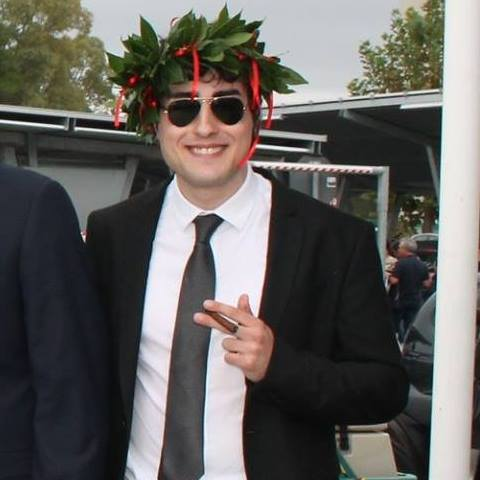
\includegraphics[width=3cm]{figures/marco.jpg}
\vspace{0.3cm}

\raisebox{-0.35ex}{
\includegraphics[width=4ex]{figures/link.png}}%
\hspace{0.05cm} /marcochiarelli

\end{figure}

\begin{figure}[h]

\includegraphics[width=3cm]{figures/gabriele.jpg}
\vspace{0.3cm}

\raisebox{-0.35ex}{
\includegraphics[width=4ex]{figures/link.png}}%
\hspace{0.05cm} /gabrieleaccarino

\end{figure}

\begin{figure}[h]

\includegraphics[width=3cm]{figures/paolo.jpg}
\vspace{0.3cm}

\raisebox{-0.35ex}{
\includegraphics[width=4ex]{figures/link.png}}%
\hspace{0.05cm} /paolo-panarese-6a016187

\end{figure}

\begin{figure}[h]

\includegraphics[width=3cm]{figures/emanuele.jpg}
\vspace{0.3cm}

\raisebox{-0.35ex}{
\includegraphics[width=4ex]{figures/link.png}}%
\hspace{0.05cm} /emanuele-costa-cesari-40ab1211a

\end{figure}


%BIBLIOGRAFIA - redatta con il relativo ambiente
\begin{thebibliography}{100}
\bibitem{rif1} G. Indiveri \emph{Notes on Rotations, Orientation Errors and Robot Kinematics}
\bibitem{rif2} G. Indiveri \emph{Introduzione alla tecnica dei Minimi Quadrati per l'identificazione parametrica e la stima dello stato}
\bibitem{rif3} G. Indiveri \emph{Ph.D Thesis, Chapter 3}
\bibitem{rif4} L. Sciavicco, B. Siciliano \emph{Robotica industriale}
\bibitem{rif5} A. Della Ducata \emph{Notazione di Denavit - Hartenberg}
\bibitem{rif6} L. Fortuna, M. Frasca \emph{Complementi di Teoria dei Sistemi e di Controlli Automatici}
\bibitem{rif7} T. I. Fossen, J. W. \& Sons \emph{Guidance and Control of Ocean Vehicles}
\bibitem{rif8} \emph{Handbook of (Marine) Robotics}
\bibitem{rif9} N. Newman \emph{Marine Hydrodynamics}
\end{thebibliography}

\end{document}
